\documentclass[10pt,a4paper,titlepage,twoside,openright]{report}
\renewcommand{\familydefault}{\sfdefault}
\usepackage{float} % for figures to appear where you want them
\usepackage{setspace}
\usepackage{graphicx}
\usepackage{changebar}
%\usepackage{glossaries}
\usepackage{pst-all}
\usepackage{pst-eucl}        %Jo
\usepackage{pst-poly}        %Jo
\usepackage{xcolor}
\usepackage{multicol}
\usepackage{pst-3dplot}        %Jo


%% ************* NB ************
%% The order in which pstricks packages are loaded
%% matters - so I copied the order from pst-all.sty
%% and then added the two additional packages at the end.
%% ************* End NB ************

%% ************* Packages ************
\usepackage{pst-circ}
\usepackage{pst-lens}
\usepackage{pst-optic}         %Jo
%\usepackage{pst-labo}         %Jo
\usepackage{subfigure}
\usepackage{multirow}
\usepackage{amsmath}
\usepackage{tabularx}
\usepackage{lscape}
\usepackage{fancyhdr}
\usepackage{wasysym}
\usepackage{url}
\usepackage{amsmath, amsthm, amsfonts, amssymb}
\usepackage{eurosym}
\usepackage{array}
\usepackage{enumitem}
\sffamily

\usepackage{mdframed}

\include{DefinitionsV0-5}

\begin{document}


\pagenumbering{roman}
\title{The Free High School Science Texts: Textbooks for High School Students Studying the Sciences\\
\textbf{Mathematics}\\
Grade 10}
\author{FHSST Authors}
\maketitle
\cleardoublepage
\begin{quote}
Copyright 2007 ``Free High School Science Texts''\\
Permission \textbf{is} granted to copy, distribute and/or modify this document under the terms of the GNU Free Documentation License, Version 1.2 or any later version published by the Free Software Foundation; with no Invariant Sections, no Front-Cover Texts, and no Back-Cover Texts.
A copy of the license is included in the section entitled ``GNU Free Documentation License''.
\end{quote}

% This is the simple stuff about the license
\begin{center}
\vspace{1.cm}
\psshadowbox[linecolor=red,linewidth=0.25cm]{{\LARGE STOP!!!!}}
\vspace{1.cm}
{\Large \\ Did you notice the FREEDOMS we've granted you?\\}
\vspace{1.cm}
\begin{quotation}{\Large Our copyright license is \textbf{different!} It grants freedoms rather than just imposing
restrictions like all those other textbooks you probably own or use.\\}\end{quotation}
{\large 
\begin{itemize} 
\item We know people copy textbooks illegally but we would LOVE it if you copied our's - 
go ahead copy to your hearts content, \textbf{legally!}
\item Publishers revenue is generated by controlling the market, we don't want any money, 
go ahead, distribute our books far and wide - we DARE you!
\item Ever wanted to change your textbook? Of course you have! Go ahead change ours, 
make your own version, get your friends together, rip it apart and put it back together 
the way you like it. That's what we really want!
\item Copy, modify, adapt, enhance, share, critique, adore, and contextualise. Do it all, 
do it with your colleagues, your friends or alone but get involved! Together we can 
overcome the challenges our complex and diverse country presents.
\item So what is the catch? The only thing you can't do is take this book, make a few changes and then tell others that they can't do the same with your changes. It's share and share-alike and we know you'll agree that is only fair.
\item These books were written by volunteers who want to help support education, who 
want the facts to be freely available for teachers to copy, adapt and re-use. Thousands 
of hours went into making them and they are a gift to everyone in the education community.
\end{itemize}
}
\end{center}

\cleardoublepage
\begin{center}{\Large FHSST Core Team\\}
Mark Horner
; Samuel Halliday 
; Sarah Blyth 
; Rory Adams
; Spencer Wheaton
\end{center}

\begin{center}{\Large FHSST Editors\\}
Jaynie Padayachee 
; Joanne Boulle
; Diana Mulcahy
; Annette Nell
; Ren\'{e} Toerien
; Donovan Whitfield
\end{center}

\begin{center}{\Large FHSST Contributors\\}

Sarah Abel
; Dr. Rory Adams
; Andrea Africa
; Ben Anhalt
; Prashant Arora
; Raymond Barbour
%; Dr. Bruce Bartlett
; Richard Baxter
; Tara Beckerling
; Tim van Beek
; Jennifer de Beyer
; Dr. Sarah Blyth
; Sebastian Bodenstein
; Martin Bongers
; Stephan Brandt
; Craig Brown
; Graeme  Broster
; Deanne de Bude
; Richard Case
; Fanny Cherblanc
; Dr. Christine Chung
; Brett Cocks
; Andrew Craig
; Tim Crombie
; Dan Crytser
; Dr. Anne  Dabrowski
; Laura Daniels
; Sean Dobbs
; Esmi Dreyer
; Matthew Duddy
; Fernando Durrell
; Dr.  Dan Dwyer
; Frans van Eeden
; Alex Ellis 
; Tom Ellis 
; Giovanni Franzoni
; Ingrid von Glehn
; Tamara von Glehn
; Lindsay Glesener
; Kevin Godby 
; Dr. Vanessa Godfrey
; Dr. Johan Gonzalez
; Hemant Gopal
; Dr. Stephanie Gould
; Umeshree Govender
; Heather Gray
; Lynn Greeff
; Dr. Tom Gutierrez
; Brooke Haag
; Kate Hadley
; Dr. Sam Halliday
; Asheena Hanuman
; Dr Melanie Dymond Harper
; Dr. Nicholas Harrison
; Neil Hart
; Nicholas Hatcher
; Dr. William P. Heal
; Pierre van Heerden
; Dr. Fritha Hennessy
; Millie Hilgart
; Chris Holdsworth
; Dr. Benne Holwerda
; Dr. Mark Horner
; Mfandaidza Hove
; Robert Hovden
; Jennifer Hsieh
; Clare Johnson
; Luke Jordan
; Tana Joseph
; Dr. Fabian Jutz
; Dr. Lutz Kampmann
; Paul Kim
; Dr. Jennifer Klay
; Lara Kruger
; Sihle Kubheka
; Andrew  Kubik
; Dr. Jannie Leach
; Dr. Marco van Leeuwen
; Dr. Tom Leinster
; Dr. Anton Machacek
; Dr. Komal Maheshwari
; Kosma von  Maltitz
; Bryony Martin
; Nicole Masureik
; John Mathew
; Dr. Will Matthews
; JoEllen McBride
; Nikolai  Meures
; Riana Meyer
; Filippo Miatto
; Jenny Miller
; Abdul Mirza
; Mapholo Modise
; Carla Moerdyk
; Asogan Moodaly
; Jothi Moodley
; David Myburgh
; Kamie Naidu
; Nolene Naidu
; Bridget Nash
; Tyrone Negus
; Thomas O'Donnell
; Dr. Markus Oldenburg
; Dr. Jaynie Padayachee
; Dave Pawson
; Nicolette Pekeur
; Sirika Pillay
; Jacques Plaut
; Andrea Prinsloo
; Joseph Raimondo
; Sanya Rajani
; Prof. Sergey Rakityansky
; Alastair Ramlakan
; Dr. Matina J. Rassias
; Dr. Jocelyn Read
; Dr. Matthew Reece
; Razvan Remsing
; Laura Richter
; Max Richter
; Sean Riddle
; Jonathan Reader
; Dr. David Roberts
; Evan Robinson
; Raoul Rontsch
; Dr. Andrew  Rose
; Katie Ross
; Jeanne-Mari\'{e} Roux
; Bianca Ruddy
; Katie Russell
; Steven Sam
; Nathaniel Schwartz
; Duncan Scott
; Helen Seals
; Ian Sherratt
; Dr. James Short
; Roger Sieloff
; Clare Slotow
; Bradley  Smith
; Greg Solomon
; Dr. Andrew Stacey
; Dr. Jim Stasheff
; Mike Stay
; Mike Stringer
; Tim Teatro
; Ben Thompson
; Shen Tian
; Nicola du Toit
; Robert Torregrosa
; Jimmy Tseng
; Pieter Vergeer
; Helen Waugh
; Dr. Dawn Webber
; Michelle Wen
; Neels van der Westhuizen
; Dr. Alexander Wetzler
; Dr. Spencer Wheaton
; Vivian White
; Dr. Gerald Wigger
; Harry Wiggins 
; Heather Williams
; Wendy Williams
; Julie Wilson
; Timothy Wilson
; Andrew Wood
; Emma Wormauld
; Dr. Sahal Yacoob
; Jean Youssef
; Ewald Zietsman
\end{center}
\singlespacing
\begin{center}
Contributors and editors have made a sincere effort to produce an accurate and useful resource. Should you have suggestions, find mistakes or be prepared to donate material for inclusion, please don't hesitate to contact us. We intend to work with all who are willing to help make this a continuously evolving resource!\\
\vspace{2cm}
{\Large www.fhsst.org}
\end{center}



% Stuff copied from thesis
% Dutch style of paragraph formatting, i.e. no indents. 
\setlength{\parskip}{1.3ex plus 0.2ex minus 0.2ex}
\setlength{\parindent}{0pt}


\pagestyle{fancy}
\renewcommand{\sectionmark}[1]{\markright{\thesection}{}}
\renewcommand{\footrulewidth}{0.4pt}

\cleardoublepage
\tableofcontents
\cleardoublepage
\pagenumbering{arabic}\part{Basics}













% CHILD SECTION START 

\chapter{Introduction to Book}
\label{mathintro}

\section{The Language of Mathematics}
The purpose of any language, like English or Zulu, is to make it possible for people to communicate. All languages have an alphabet, which is a group of letters that are used to make up words. There are also rules of grammar which explain how words are supposed to be used to build up sentences. This is needed because when a sentence is written, the person reading the sentence understands exactly what the writer is trying to explain. Punctuation marks (like a full stop or a comma) are used to further clarify what is written.

Mathematics is a language, specifically it is the language of Science. Like any language, mathematics has letters (known as numbers) that are used to make up words (known as expressions), and sentences (known as equations). The punctuation marks of mathematics are the different signs and symbols that are used, for example, the plus sign (+), the minus sign (-), the multiplication sign ($\times$), the equals sign (=) and so on. There are also rules that explain how the numbers should be used together with the signs to make up equations that express some meaning.

%\section{Structure of Book}
%This book is divided into four parts, according to the four learning outcomes required by the National %Curriculum Statement for Mathematics (Grades 10 - 12). For the final Grade 12 examination, Parts 1 and 2 %will be examined in the first examination paper and Parts 3 and 4 will be examined in the second examination %paper.

%Each section in the text is marked as being for Grades 10, 11 or 12 and extra content not in the syllabus is %marked as \textbf{Advanced}. Where no indication of grade is given, these sections are to be considered as %introductory sections and are applicable for all grades, to clarify the content.

%The book is structured as follows:

%\begin{itemize}
%\item{\textbf{Building a Solid Foundation} contains a brief overview of key concepts that the reader should %be comfortable with, before the rest of the book is attempted.}
%\item{Part 1 - Learning Outcome 1: Numbers and Number Relationships}
%\begin{itemize}
%\item{Chapter: Numbers}
%\item{Chapter: Patterns in Numbers}
%\item{Chapter: Finance}
%\end{itemize}
%\item{Part 2 - Learning Outcome 2: Functions and Algebra}
%\begin{itemize}
%\item{Chapter: Functions and Graphs}
%\item{Chapter: Solving Equations}
%\item{Chapter: Differentiation}
%\item{Chapter: Linear Programming}
%\end{itemize}
%\item{Part 3 - Learning Outcome 3: Space, Shape and Measurement}
%\begin{itemize}
%\item{Chapter: Geometry}
%\item{Chapter: Trigonometry}
%\end{itemize}
%\begin{itemize}
%\item{Part 4 - Learning Outcome 4: Data Handling and Probability}
%\item{Chapter: Statistics}
%\item{Chapter: Probability}
%\item{Chapter: Combinations and Permutations}
%\end{itemize}
%\end{itemize}



%\section{How this book should be used}
%\nts{List how we see the book being used.}

% CHILD SECTION END 



% CHILD SECTION START 

\part{Grade 10}

% CHILD SECTION START 

\chapter{Review of Past Work}
\label{mfoundation}

\section{Introduction}
This chapter describes some basic concepts which you have seen in earlier grades, and lays the foundation for the remainder of this book. You should feel confident with the content in this chapter, before moving on with the rest of the book. 

So try out your skills on the exercises throughout this chapter and ask your teacher for more questions just like them. You can also try making up your own questions, solve them and try them out on your classmates to see if you get the same answers.

Practice is the only way to get good at maths!


\section{What is a number?}
A number is a way to represent quantity. Numbers are not something that you can touch or hold, because they are not physical. But you can touch three apples, three pencils, three books. You can never just touch three, you can only touch three of something. However, you do not need to see three apples in front of you to know that if you take one apple away, that there will be two apples left. You can just think about it. That is your brain representing the apples in numbers and then performing arithmetic on them.

A number represents quantity because we can look at the world around us and
quantify it using numbers. How many minutes? How many kilometers? How
many apples? How much money? How much medicine? These are all questions which can only be answered using numbers to tell us ``how much'' of something we want to measure.

A number can be written many different ways and it is always best to choose the most appropriate way of writing the number. For example, ``a half'' may be spoken aloud or written in words, but that makes mathematics very difficult and also means that only people who speak the same language as you can understand what you mean. A better way of writing ``a half'' is as a fraction $\frac{1}{2}$ or as a decimal number $0,5$. It is still the same number, no matter which way you write it.

In high school, all the numbers which you will see are called \textit{real
numbers} and mathematicians use the symbol $\mathbb R$ to stand for the \textit{set of all real numbers}, which simply means all of the real numbers. Some of these real numbers can be written in ways that others cannot. Different types of numbers are described in detail in Section 1.12.


\section{Sets}
A \textit{set} is a group of objects with a well-defined criterion for membership. For example, the criterion for belonging to a set of apples, is that the object must be an apple. The set of apples can then be divided into red apples and green apples, but they are all still apples. All the red apples form another set which is a \textit{sub-set} of the set of apples. A sub-set is part of a set. All the green apples form another sub-set. 
 
Now we come to the idea of a \textbf{union}, which is used to combine things. The symbol for \textbf{union} is $\cup$. Here we use it to combine two or more intervals. For example, if $x$ is a real number such that $1 < x \leq 3$ or $6 \leq x < 10$, then the set of all the possible $x$ values is
\begin{equation}
  \label{eq:mf:g:interval}
    (1,3]\cup[6,10)
\end{equation}
where the $\cup$ sign means the union (or combination) of the two intervals.  We use the set and interval notation and the symbols described because it is easier than having to write everything out in words.



\section{Letters and Arithmetic}
\label{mfoundation:alg}
The simplest things that can be done with numbers is to add, subtract, multiply or divide them. When two numbers are added, subtracted, multiplied or divided, you are performing \textit{arithmetic}\footnote{Arithmetic is derived from the Greek word \textit{arithmos} meaning \textit{number}.}. These four basic operations can be performed on any two real numbers.

Mathematics as a language uses special notation to write things down. So instead of:
\nequ{\mbox{one plus one is equal to two}}
mathematicians write
\nequ{1+1=2}

In earlier grades, place holders were used to indicate missing numbers in an equation.
\begin{eqnarray*}
1+\Box=2\\
4-\Box=2\\
\Box+3-2\Box=2
\end{eqnarray*}

However, place holders only work well for simple equations. For more advanced mathematical workings, letters are usually used to represent numbers. 
\begin{eqnarray*}
\label{min:variables}
1+x=2\\
4-y=2\\
z+3-2z=2
\end{eqnarray*}

These letters are referred to as \textbf{variables}, since they can take on any value depending on what is required. For example, $x=1$ in Equation~\ref{min:variables}, but $x=26$ in $2+x=28$.
\\
A \textbf{constant} has a fixed value. The number 1 is a constant. The \textit{speed of light} in a vacuum is also a constant which has been defined to be exactly 299 792 458 \ms (read metres per second). The speed of light is a big number and it takes up space to always write down the entire number. Therefore, letters are also used to represent some constants. In the case of the speed of light, it is accepted that the letter $c$ represents the speed of light. Such constants represented by letters occur most often in physics and chemistry.

Additionally, letters can be used to describe a situation, mathematically. For example, the following equation
\begin{equation}
\label{eq:mfoundation:alg:ex1}
x+y=z
\end{equation}
can be used to describe the situation of finding how much change can be expected for buying an item. In this equation, $y$ represents the price of the item you are buying, $x$ represents the amount of change you should get back and $z$ is the amount of money given to the cashier. So, if the price is R10 and you gave the cashier R15, then write R15 instead of $z$ and R10 instead of $y$ and the change is then $x$.
\begin{equation}
x+10=15
\end{equation}

We will learn how to ``solve'' this equation towards the end of this chapter.

\section{Addition and Subtraction}
\label{mfoundation:alg:a}
Addition (+) and subtraction (-) are the most basic operations between numbers but they are very closely related to each other. You can think of subtracting as being the opposite of adding since adding a number and then subtracting the same number will not change what you started with. For example, if we start with $a$ and add $b$, then subtract $b$, we will just get back to
$a$ again:
\begin{eqnarray}
  \label{eq:mfoundation:alg:a:addsub}
  a+b-b=a\\ \nonumber
  5+2-2=5
\end{eqnarray}

If we look at a number line, then addition means that we move to the right and subtraction means that we move to the left.

The order in which numbers are added does not matter, but the order in which numbers are subtracted does matter. This means that:
\begin{eqnarray}
  \label{eq:mfoundation:alg:a:associativityadd}
  a+b&=&b+a\\ \nonumber
  a-b&\neq&b-a \quad \mbox{if $a \neq b$}
\end{eqnarray}
The sign $\neq$ means ``is not equal to''. For example, $2+3=5$ and $3+2=5$, but $5-3=2$ and $3-5=-2$. $-2$ is a negative number, which is explained in detail in Section \ref{mfoundation:negative}.

\Extension{Commutativity for Addition}{The fact that $a+b=b+a$, is known as the
\textit{commutative} property for addition.}

\section{Multiplication and Division}
\label{mfoundation:alg:m}
Just like addition and subtraction, multiplication ($\times$, $\cdot$) and
division ($\div$, /) are opposites of each other. Multiplying by a number and
then dividing by the same number gets us back to the start again:
\begin{eqnarray}
  \label{eq:mfoundation:alg:m:multdiv}
  a\times b\div b=a\\ \nonumber
  5\times 4\div 4=5
\end{eqnarray}

Sometimes you will see a multiplication of letters as a dot or 
without any symbol. Don't worry, its exactly the same thing. Mathematicians are
efficient and like to write things in the shortest, neatest way possible.
\begin{eqnarray}
  \label{eq:mfoundation:alg:m:nox}
  abc&=&a\times b\times c\\
a \cdot b \cdot c&=&a\times b\times c \nonumber
\end{eqnarray}

It is usually neater to write known numbers to the left, and letters to the
right. So although $4x$ and $x4$ are the same thing, it looks better to
write $4x$. In this case, the ``4'' is a constant that is referred to as the
\textit{coefficient} of $x$.

\Extension{Commutativity for Multiplication}{The fact that $ab=ba$ is known as
the \textit{commutative} property of multiplication. Therefore, both addition
and multiplication are described as commutative operations.}

\section{Brackets}
\label{mfoundation:alg:b}
Brackets\footnote{Sometimes people say ``parentheses'' instead of ``brackets''.}
in mathematics are used to show the order in which you must do things. This is
important as you can get different answers depending on the order in which you
do things. For example 
\begin{equation}
  \label{eq:mfoundation:alg:b:parenth1}
  (5\times 5) + 20 = 45
\end{equation}
whereas
\begin{equation}
  \label{eq:mfoundation:alg:b:parenth2}
  5\times (5 + 20) = 125
\end{equation}
If there are no brackets, you should always do multiplications and
divisions first and then additions and subtractions\footnote{Multiplying and
dividing can be performed in any order as it doesn't matter. Likewise it
doesn't matter which order you do addition and subtraction. Just as long as
you do any $\times\div$ before any $+-$.}. You can always put your own brackets
into equations using this rule to make things easier for yourself,  for example:
\begin{eqnarray}
  \label{eq:mfoundation:alg:b:parenth3}
  a\times b + c \div d &=& (a\times b) + (c\div d)\\ \nonumber
  5\times 5 + 20 \div 4 &=& (5\times 5) + (20\div 4)
\end{eqnarray}

If you see a multiplication outside a bracket like this
\begin{eqnarray}
  \label{eq:mfoundation:alg:m:bra}
  a(b+c)\\ \nonumber
  3(4-3)
\end{eqnarray}
then it means you have to multiply each part inside the bracket by the number
outside
\begin{eqnarray}
  \label{eq:mfoundation:alg:m:bra2}
  a(b+c)&=&ab+ac\\ \nonumber
  3(4-3)&=&3\times4-3\times3=12-9=3
\end{eqnarray}
unless you can simplify everything inside the bracket into a single term. In
fact, in the above example, it would have been smarter to have done this
\begin{equation}
  \label{eq:mfoundation:alg:m:bra3}
  3(4-3)=3\times(1)=3
\end{equation}
It can happen with letters too
\begin{equation}
  \label{eq:mfoundation:alg:m:bra4}
  3(4a-3a)=3\times(a)=3a
\end{equation}

\Extension{Distributivity}{The fact that $a(b+c)=ab+ac$ is known as the
\textit{distributive} property.}

If there are two brackets multiplied by each other, then you can do it one step
at a time:
\begin{eqnarray}
  \label{eq:mfoundation:alg:m:sqbra}
  (a+b)(c+d)&=&a(c+d) + b(c+d)\\ \nonumber
  &=& ac+ad+bc+bd\\ \nonumber
  (a+3)(4+d)&=&a(4+d) + 3(4+d)\\ \nonumber
  &=& 4a+ad+12+3d
\end{eqnarray}

\section{Negative Numbers}
\label{mfoundation:negative}

\subsection{What is a negative number?}
Negative numbers can be very confusing to begin with, but there is nothing to be
afraid of. The numbers that are used most often are greater than zero. These
numbers are known as \textit{positive numbers}. 

A negative number is a number that is less than zero. So, if we were to
take a positive number $a$ and subtract it from zero, the answer would be the
negative of $a$.
\nequ{0-a=-a}

On a number line, a negative number appears to the left of zero and a positive
number appears to the right of zero.

\begin{figure}[htb]
\begin{center}
\begin{pspicture}(-4,0.75)(4,1.75)
%\psgrid
\psline[arrows=<->](-4,1)(4,1)
\uput[d](-1,1){-1}
\uput[d](-2,1){-2}
\uput[d](-3,1){-3}
\uput[d](0,1){0}
\uput[d](1,1){1}
\uput[d](2,1){2}
\uput[d](3,1){3}
\psline(0,1.1)(0,0.9)
\psline(1,1.1)(1,0.9)
\psline(2,1.1)(2,0.9)
\psline(3,1.1)(3,0.9)
\psline(-1,1.1)(-1,0.9)
\psline(-2,1.1)(-2,0.9)
\psline(-3,1.1)(-3,0.9)
\psline[arrows=<-](-1,1.5)(0,1.5)
\psline[arrows=->](0,1.5)(1,1.5)
\psline(0,1.4)(0,1.6)
\uput[r](1,1.5){positive numbers}
\uput[l](-1,1.5){negative numbers}
\end{pspicture}
\caption{On the number line, numbers increase towards the right and decrease
towards the left. Positive numbers appear to the right of zero and negative
numbers appear to the left of zero.\label{fig:mfoundation:nl}}
\end{center}
\end{figure}

\subsection{Working with Negative Numbers}

When you are adding a negative number, it is the same as subtracting that number
if it were positive. Likewise, if you subtract a negative number, it is the same
as adding the number if it were positive. Numbers are either positive or
negative, and we call this their {\textit sign}. A positive number has positive
sign ($+$), and a negative number has a negative sign ($-$).

Subtraction is actually the same as adding a \textit{negative number}. 

In this example, $a$ and $b$ are positive numbers, but $-b$ is a negative number
\begin{eqnarray}
  \label{eq:mfoundation:alg:a:addneg}
  a-b=a+(-b)\\ \nonumber
  5-3=5+(-3)
\end{eqnarray}

So, this means that subtraction is simply a short-cut for adding a negative
number, and instead of writing $a+(-b)$, we write $a-b$. This also means that
$-b+a$ is the same as $a-b$. Now, which do you find easier to work out?

Most people find that the first way is a bit more difficult to work out than the
second way. For example, most people find $12-3$ a lot easier to work out than
$-3+12$, even though they are the same thing. So, $a-b$, which looks neater and
requires less writing, is the accepted way of writing subtractions. 

Table \ref{tab:n:alg:multsgn} shows how to calculate the sign of the answer when
you multiply two numbers together. The first column shows the sign of the first
number, the second column gives the sign of the second number, and the third
column shows what sign the answer will be.
\begin{table}[!h]
  \centering
  \begin{tabular}{|c|c|c|}\hline
    $a$ & $b$ & $a\times b$ or $a\div b$\\\hline\hline
    $+$ & $+$ & $+$ \\\hline
    $+$ & $-$ & $-$ \\\hline
    $-$ & $+$ & $-$ \\\hline
    $-$ & $-$ & $+$\\\hline
  \end{tabular}
  \caption{Table of signs for multiplying or dividing two numbers.}
  \label{tab:n:alg:multsgn}
\end{table}
So multiplying or dividing a negative number by a positive number always gives
you a negative number, whereas multiplying or dividing numbers which have the
same sign always gives a positive number. For example, $2\times3=6$ and
$-2\times-3=6$, but $-2\times3=-6$ and $2\times-3=-6$.

Adding numbers works slightly differently (see Table
\ref{tab:n:alg:addsgn}). The first column shows the sign of the first number, the
second column gives the sign of the second number, and the third column shows
what sign the answer will be.

\begin{table}[!h]
  \centering
  \begin{tabular}{|c|c|c|}\hline
    $a$ & $b$ & $a+b$\\\hline\hline
    $+$ & $+$ & $+$ \\\hline
    $+$ & $-$ & ? \\\hline
    $-$ & $+$ & ? \\\hline
    $-$ & $-$ & $-$\\\hline
  \end{tabular}
  \caption{Table of signs for adding two numbers.}
  \label{tab:n:alg:addsgn}
\end{table}
If you add two positive numbers you will always get a positive number, but if
you add two negative numbers you will always get a negative number. If the
numbers have different sign, then the sign of the answer depends on which one is
bigger.

\subsection{Living Without the Number Line}
The number line in Figure~\ref{fig:mfoundation:nl} is a good way to visualise
what negative numbers are, but it can get very inefficient to use it every time
you want to add or subtract negative numbers. To keep things simple, we will
write down three tips that you can use to make working with negative numbers a
little bit easier. These tips will let you work out what the answer is when you
add or subtract numbers which may be negative and will also help you keep your
work tidy and easier to understand.

%\nts{JP:  Have changed these to `Tips', which sounds more friendly than
%`Rules'. I also think that Tips gives the impression of making a kid's life
%easier, whereas Rules are usually there to complicate things.}

\subsubsection{Negative Numbers Tip 1}
If you are given an expression like $-a+b$, then it is easier to move the numbers
around so that the expression looks easier. For this case, we have seen that
adding a negative number to a positive number is the same as subtracting the
number from the positive number. So,
\begin{eqnarray}
  \label{eq:mfoundation:alg:rule1}
  -a+b &=& b-a \\ \nonumber
  -5 + 10 &=& 10 + (- 5) \\ \nonumber
          &=& 10 - 5 \\ \nonumber
          &=& 5
\end{eqnarray}
This makes expression easier to understand. For example, a question like ``What
is $-7+11$?'' looks a lot more complicated than ``What is $11-7$?'', even though
they are exactly the same question.

\subsubsection{Negative Numbers Tip 2}
When you have two negative numbers like $-3-7$, you can calculate the answer by
simply adding together the numbers as if they were positive and then putting a
negative sign in front.
\begin{eqnarray}
  \label{eq:mfoundation:alg:rule2}
  -c-d &=& -(c+d)\\ \nonumber
  -7 - 2 &=& -(7+2) = -9
\end{eqnarray}

\subsubsection{Negative Numbers Tip 3}
In Table \ref{tab:n:alg:addsgn} we saw that the sign of two numbers added
together depends on which one is bigger. This tip tells us that all we need to
do is take the smaller number away from the larger one, and remember to give 
the answer the sign of the larger number. In this equation, $F$ is bigger than $e$.

\begin{eqnarray}
  \label{eq:mfoundation:alg:rule3}
  e-F &=& -(F-e)\\ \nonumber
  2 - 11 &=& -(11-2) = -9
\end{eqnarray}

You can even combine these tips together, so for example you can use Tip 1 on
$-10+3$ to get $3-10$, and then use Tip 3 to get $-(10-3)=-7$.

\Exercise{Negative Numbers}{
\begin{enumerate}
\item{Calculate:

\centering
\begin{tabular}{lll}
(a)  $(-5)-(-3)$ & (b)  $(-4)+2$ & (c)  $(-10)\div(-2)$ \\
(d)  $11-(-9)$ & (e)  $-16-(6)$ & (f) $-9\div3 \times  2$\\
(g)  $(-1) \times  24\div8 \times (-3)$ & (h)  $(-2)+(-7)$ & (i)  $1-12$\\
(j)  $3-64+1$ & (k)  {$-5-5-5$} & (l)  {$-6+25$}\\
(m)  {$-9+8-7+6-5+4-3+2-1$}&&\\
\end{tabular}}
\item{Say whether the sign of the answer is $+$ or $-$

\centering
\begin{tabular}{lll}
(a) {$-5 +6$} & (b)  {$-5 +1$} & (c)  {$-5 \div -5$}\\
(d)  {$-5 \div 5$} & (e)  {$5 \div -5$} & (f)  {$5 \div 5$}\\
(g)  {$-5 \times -5$} & (h)  {$-5 \times 5$} & (i)  {$5 \times -5$}\\
(j)  {$5 \times 5$}&&\\
\end{tabular}}
\end{enumerate}}



\section{Rearranging Equations}
\label{mfoundation:alg:r}
Now that we have described the basic rules of negative and positive numbers and
what to do when you add, subtract, multiply and divide them, we are ready to
tackle some real mathematics problems!

Earlier in this chapter, we wrote a general equation for calculating how much
change ($x$) we can expect if we know how much an item costs ($y$) and how much
we have given the cashier ($z$).  The equation is:
\begin{equation}
x+y=z
\end{equation}
So, if the price is R10 and you gave the cashier R15, then write R15 instead of
$z$ and R10 instead of $y$.
\begin{equation}
x+10=15
\end{equation}
Now that we have written this equation down, how exactly do we go about finding
what the change is? In mathematical terms, this is known as solving an equation
for an unknown ($x$ in this case). We want to re-arrange the terms in the
equation, so that only $x$ is on the left hand side of the $=$ sign and
everything else is on the right.

The most important thing to remember is that an equation is like a set of
weighing scales. In order to keep the scales balanced, whatever, is done to one
side, must be done to the other. 

\begin{figure}[htb]
\begin{center}
\begin{pspicture}(-5,-5)(5,5)
%\psgrid[subgriddiv=1,griddots=10,gridlabels=10pt]
\psellipse[fillstyle=solid,fillcolor=black](0,4)(2.5,0.05)
\pspolygon[fillstyle=solid,fillcolor=black](-0.25,0.5)(0.25,0.5)(0,4.5)
\psframe[fillstyle=solid,fillcolor=black](-0.5,0)(0.5,0.5)
\psline(-2,4)(-3,2)
\psline(-2,4)(-1,2)
\psline(2,4)(3,2)
\psline(2,4)(1,2)
\psarc[linewidth=5pt,arrows=*-*](-2,2.5){1.03}{200}{340}
\uput[u](-2,1.5){$x+y$}
\psarc[linewidth=5pt,arrows=*-*](2,2.5){1.03}{200}{340}
\uput[u](2,1.5){$z$}
\rput(0,-5){\psellipse[fillstyle=solid,fillcolor=black](0,4)(2.5,0.05)
\pspolygon[fillstyle=solid,fillcolor=black](-0.25,0.5)(0.25,0.5)(0,4.5)
\psframe[fillstyle=solid,fillcolor=black](-0.5,0)(0.5,0.5)
\psline(-2,4)(-3,2)
\psline(-2,4)(-1,2)
\psline(2,4)(3,2)
\psline(2,4)(1,2)
\psarc[linewidth=5pt,arrows=*-*](-2,2.5){1.03}{200}{340}
\uput[u](-2,1.7){$x+y-y$}
\psarc[linewidth=5pt,arrows=*-*](2,2.5){1.03}{200}{340}
\uput[u](2,1.7){$z-y$}}
\end{pspicture}
\caption{An equation is like a set of weighing scales. In order to keep the
scales balanced, you must do the same thing to both sides. So, if you add,
subtract, multiply or divide the one side, you must add, subtract, multiply or
divide the other side too.}
\label{fig:mfoundation:scales}
\end{center}
\end{figure}


%\begin{figure}[!h]
%\begin{center}
%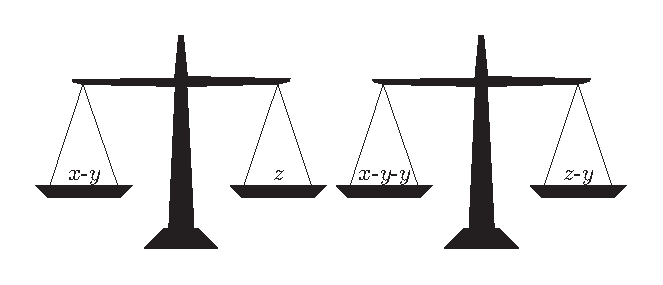
\includegraphics[width=4in]{ch1scales.eps}
%\caption{An equation is like a set of weighing scales. In order to keep the
%scales balanced, you must add the same quantity to both sides.}
%\label{fig:mfoundation:scales}
%\end{center}
%\end{figure}

\subsubsection{Method: Rearranging Equations}{

You can add, subtract, multiply or divide both sides of an equation by any
number you want, as long as you always do it to both sides.} 

So for our example we could subtract $y$ from both sides
\begin{eqnarray}
  \label{eq:mfoundation:alg:r:change}
  x+y&=&z \\ \nonumber
  x+y-y&=&z-y\\ \nonumber
  x&=&z-y\\ \nonumber
  x&=&15-10\\  \nonumber
	&=&5
\end{eqnarray}
Now we can see that the change is the price subtracted from the amount paid
to the cashier. In the example, the change should be R5. In real life we
can do this in our heads; the human brain is very smart and can do arithmetic
without even knowing it.

When you subtract a number from both sides of an equation, it looks just like
you moved a positive number from one side and it became a negative on the other,
which is exactly what happened. Likewise if you move a multiplied number from
one side to the other, it looks like it changed to a divide. This is because you
really just divided both sides by that number, and a number divided by itself is
just $1$
\begin{eqnarray}
  \label{eq:mfoundation:alg:r:mult}
  a(5+c)&=&3a\\ \nonumber
  a(5+c)\div a&=&3a\div a\\ \nonumber
  \frac{a}{a} \times (5+c)&=&3\times \frac{a}{a}\\ \nonumber
  1\times(5+c)&=&3\times 1\\ \nonumber
  5+c&=& 3\\ \nonumber
  c&=&3-5=-2
\end{eqnarray}
However you must be careful when doing this, as it is easy to make mistakes.

\textbf{The following is the WRONG thing to do}
\begin{eqnarray}
  \label{eq:mfoundation:alg:r:multwrong}
  5a+c&=&3a\\ \nonumber
   5+c&=&3 
  %5+c&\neq\footnote{The $\neq$
%symbol says that this is incorrect as it means ``not equal to''.} &3a\div a
\end{eqnarray}
Can you see why it is wrong? It is wrong because we did not divide the $c$ term
by $a$ as well. The correct thing to do is 
\begin{eqnarray}
  \label{eq:mfoundation:alg:r:multcorrect}
  5a+c&=&3a\\ \nonumber
  5+c\div a&=&3\\ \nonumber
  c\div a&=& 3-5=-2
\end{eqnarray}

\Exercise{Rearranging Equations}{
\begin{enumerate}
\item{If $3(2r-5)= 27$, then $2r-5 = .....$}
\item{Find the value for $x$ if $0,5(x-8)= 0,2x+11$}
\item{Solve $9 - 2n = 3(n + 2)$}
\item{Change the formula $P=A+Akt$  to $A = $}
\item{Solve for $x$: $\frac{1}{ax}+\frac{1}{bx}=1$}
\end{enumerate}
}

\section{Fractions and Decimal Numbers}
\label{mfoundation:fd}
A fraction is one number divided by another number. There are several ways to
write a number divided by another one, such as $a\div b$, $a/b$ and $\frac ab$.
The first way of writing a fraction is very hard to work with, so we will use
only the other two. We call the number on the top (left) the \textit{numerator} and
the number on the bottom (right) the \textit{denominator}. For example, in the fraction
$1/5$ or $\frac{1}{5}$, the numerator is 1 and the denominator is 5.

\Extension{Definition - Fraction}{The word \textit{fraction} means \textit{part
of a whole}.}

The \textit{reciprocal} of a fraction is the fraction turned upside down, in
other words the numerator becomes the denominator and the denominator becomes
the numerator. So, the reciprocal of $\frac{2}{3}$ is $\frac{3}{2}$.
\\
A fraction multiplied by its reciprocal is always equal to $1$ and can be
written
\begin{equation}
\label{eq:mfoundation:fd:recip}
\frac{a}{b}\times\frac{b}{a} = 1
\end{equation}
This is because dividing by a number is the same as multiplying by its
reciprocal. 

\Extension{Definition - Multiplicative Inverse}{The reciprocal of a number is
also known as the multiplicative inverse.}

A decimal number is a number which has an integer part and a fractional part.
The integer and the fractional parts are separated by a \textit{decimal point},
which is written as a comma in South African schools. For example the number $3
\frac{14}{100}$ can be written much more cleanly as $3,14$.

All real numbers can be written as a decimal number. However, some numbers would
take a huge amount of paper (and ink) to write out in full! Some decimal numbers
will have a number which will repeat itself, such as $0,33333\ldots$ where there
are an infinite number of 3's. We can write this decimal value by using a dot
above the repeating number, so $0,\Dot3 = 0,33333\ldots$. If there are two
repeating numbers such as $0,121212\ldots$ then you can place dots\footnote{or a
bar, like $0,\overline{12}$} on each of the repeated numbers
$0,\dot1\dot2=0,121212\ldots$. These kinds of repeating decimals are called
\textit{recurring decimals}.

Table \ref{tab:mfoundation:fd:common} lists some common fractions and their
decimal forms.

\begin{table}
\begin{center}
\begin{tabular}{|c|c|}
\hline
Fraction & Decimal Form\\\hline
\hline
$\frac{1}{20}$ & 0,05\\
\\
$\frac{1}{16}$ & 0,0625\\
\\
$\frac{1}{10}$ & 0,1\\
\\
$\frac{1}{8}$ & 0,125\\
\\
$\frac{1}{6}$ & $0,16\dot6$\\
\\
$\frac{1}{5}$ & 0,2\\
\\
$\frac{1}{2}$ & 0,5\\
\\
$\frac{3}{4}$ & 0,75\\
\\
\hline
\end{tabular}
\caption{Some common fractions and their equivalent decimal forms.}
\label{tab:mfoundation:fd:common}
\end{center}
\end{table}

\section{Scientific Notation}
In science one often needs to work with very large or very small numbers. These
can be written more easily in scientific notation, which has the general form
\begin{equation}
\label{mn:a:sci}
a \times 10^m
\end{equation}
where $a$ is a decimal number between 0 and 10 that is rounded off to a few
decimal places. The $m$ is an integer and if it is positive it represents how
many zeros should appear to the right of $a$. If $m$ is negative then it
represents how many times the decimal place in $a$ should be moved to the left.
For example $3,2\times 10^3$ represents 32~000 and $3,2\times 10^{-3}$ represents
$0,0032$.

If a number must be converted into scientific notation, we need to work out how
many times the number must be multiplied or divided by 10 to make it into a
number between 1 and 10 (i.e. we need to work out the value of the exponent $m$)
and what this number is (the value of $a$). We do this by counting the number of
decimal places the decimal point must move. 

For example, write the speed of light which is 299~792~458~ms$^{-1}$ in
scientific notation, to two decimal places. First, determine where the decimal
point must go for two decimal places (to find $a$) and then count how many
places there are after the decimal point to determine $m$.

In this example, the decimal point must go after the first 2, but since the
number after the 9 is a 7, $a=3,00$. 

So the number is $3,00 \times 10^{m}$, where $m=8$, because there are 8 digits
left after the decimal point. So the speed of light in scientific notation, to
two decimal places is $3,00 \times 10^{8} $~ms$^{-1}$.

As another example, the size of the HI virus is around $1,2\times10^{-7}$~m.
This is equal to $1,2\times 0,0000001$~m which is 0,00000012~m.


\section{Real Numbers}
Now that we have learnt about the basics of mathematics, we can look at what
real numbers are in a little more detail. The following are examples of real
numbers and it is seen that each number is written in a different way. 
\begin{equation}
\sqrt{3},\quad 1,2557878,\quad \frac{56}{34},\quad 10,\quad 2,1,\quad -5,\quad
-6,35, \quad -\frac{1}{90}
\end{equation}

Depending on how the real number is written, it can be further labelled as
either rational, irrational, integer or natural. A set diagram of the different
number types is shown in Figure~\ref{fig:mfoundation:r:numbertypes}.

\begin{figure}[!ht]
\begin{center}
\begin{pspicture}(-2.6,-2.0)(2.6,2.0)
\psellipse(0,0)(2.5,2.0)
\rput(1.85,0){$\mathbb R$}
\psellipse[fillstyle=vlines](-0.6,0)(1.2,1)
\psellipse[fillstyle=hlines](-0.5,0)(1.8,1.7)
\psellipse[fillstyle=solid,linecolor=white,fillcolor=white](0.9,0)(0.2,0.2)
\rput(0.9,0){$\mathbb Q$}
\psellipse[fillstyle=solid,linecolor=white](0.2,0)(0.2,0.2)
\rput(0.2,0){$\mathbb Z$}
\psellipse[fillstyle=solid,fillcolor=lightgray](-0.8,0)(.7,0.6)
%\psellipse[fillstyle=solid,fillcolor=lightgray](-0.4,0)(0.2,0.2)
\rput(-0.4,0){$\mathbb N$}
\end{pspicture}
\caption{Set diagram of all the real numbers $\mathbb R$, the rational
numbers $\mathbb Q$, the integers $\mathbb Z$ and the natural numbers $\mathbb
N$. The irrational numbers are the numbers not inside the set of rational
numbers. All of the integers are also rational numbers, but not all rational
numbers are integers.}
\label{fig:mfoundation:r:numbertypes}
\end{center}
\end{figure}

\Extension{Non-Real Numbers}{All numbers that are not real numbers have
\textit{imaginary} components. We will not see imaginary  numbers in this book
but they come from $\sqrt{-1}$. Since we won't be looking at
numbers which are not real, if you see a number you can be sure it is a real
one.}

\subsection{Natural Numbers}
\label{mfoundation:n}
The first type of numbers that are learnt about are the numbers that are used
for counting.  These numbers are called \textit{natural numbers} and are the
simplest numbers in mathematics: 
\begin{equation}
\label{eq:mfoundation:nm:nat}
0, 1, 2, 3, 4,\ldots
\end{equation}
Mathematicians use the symbol $\mathbb N_0$ to mean the \textit{set of all natural
numbers}. These are also sometimes called \textit{whole numbers}. The natural numbers are a \textit{subset} of the real numbers since
every natural number is also a real number. 

\subsection{Integers}
\label{mfoundation:i}
The integers are all of the natural numbers and their negatives:
\begin{equation}
\label{eq:mfoundation:nm:int}
\ldots-4, -3, -2, -1, 0, 1, 2, 3, 4\ldots
\end{equation}
Mathematicians use the symbol $\mathbb Z$ to mean \textit{the set of all
integers}. The integers are a subset of the real numbers, since every integer is
a real number.

\subsection{Rational Numbers}
\label{mfoundation:r}
The natural numbers and the integers are only able to describe quantities that
are whole or complete. For example you can have 4 apples, but what happens when
you divide one apple into 4 equal pieces and share it among your friends? Then
it is not a whole apple anymore and a different type of number is needed to
describe the apples. This type of number is known as a rational number.

A rational number is any number which can be written as:
\begin{equation}
\label{eq:r:rational}
\frac{a}{b}
\end{equation}
where $a$ and $b$ are integers and $b\ne 0$.

The following are examples of rational numbers:
\begin{equation}
\label{eq:r:rationalexamples}
\frac{20}{9}, \quad \frac{-1}{2}, \quad \frac{20}{10}, \quad \frac{3}{15}
\end{equation}


\Extension{Notation Tip}{Rational numbers are any number that can be expressed
in the form $\frac{a}{b}; a, b \in \mathbb Z; b \neq 0$ which means ``the set of
numbers $\frac{a}{b}$ when $a$ and $b$ are integers''.}

Mathematicians use the symbol $\mathbb Q$ to mean \textit{the set of all
rational numbers}. The set of rational numbers contains all numbers which can be
written as terminating or repeating decimals. 

\Extension{Rational Numbers}{All integers are rational numbers with denominator
$1$.}

You can add and multiply rational numbers and still get a rational number at the
end, which is very useful. If we have 4 integers, $a, b, c$ and $d$, then the
rules for adding and multiplying rational numbers are
\begin{eqnarray}
\label{eq:mfoundation:r:add}
\frac ab + \frac cd &=& \frac{ad+bc}{bd}\\
\label{eq:mfoundation:r:mult}
\frac ab \times \frac cd &=& \frac{ac}{bd}
\end{eqnarray}

\Extension{Notation Tip}{The statement "4 integers $a, b, c$ and $d$" can be
written formally as $\{a, b, c, d\}\in \mathbb Z$ because the $\in$ symbol means
\textit{in} and we say that $a, b, c$ and $d$ are \textit{in} the set of
integers.}

Two rational numbers ($\frac ab$ and $\frac cd$) represent the same number if $ad=bc$. It is always best to simplify any rational number so that the
denominator is as small as possible. This can be achieved by dividing both the numerator and the denominator by the same integer. For example, the rational number $1000/10000$ can be divided by 1000 on the top and the bottom, which gives $1/10$. $\frac{2}{3}$ of a pizza is the same as $\frac{8}{12}$ (Figure~\ref{fig:mfoundation:pizza}).


\begin{figure}[htb]
\begin{center}
\begin{pspicture}(-4,-2)(4,2.8)
%\psgrid
\rput(-2,0){\pswedge[fillcolor=lightgray,fillstyle=solid](0,0){1.75}{0}{30}
\pswedge[fillcolor=lightgray,fillstyle=solid](0,0){1.75}{30}{60}
\pswedge[fillcolor=lightgray,fillstyle=solid](0,0){1.75}{60}{90}
\pswedge[fillcolor=lightgray,fillstyle=solid](0,0){1.75}{90}{120}
\pswedge[fillcolor=lightgray,fillstyle=solid](0,0){1.75}{120}{150}
\pswedge[fillcolor=lightgray,fillstyle=solid](0,0){1.75}{150}{180}
\pswedge[fillcolor=lightgray,fillstyle=solid](0,0){1.75}{180}{210}
\pswedge[fillcolor=lightgray,fillstyle=solid](0,0){1.75}{210}{240}
\pswedge(0,0){1.75}{240}{270}
\pswedge(0,0){1.75}{270}{300}
\pswedge(0,0){1.75}{300}{330}
\pswedge(0,0){1.75}{330}{360}
\psarc[linewidth=1.5pt,arrows=|->](0,0){1.90}{0}{240}}
\rput(2,0){\pswedge[fillcolor=lightgray,fillstyle=solid](0,0){1.75}{0}{120}
\pswedge[fillcolor=lightgray,fillstyle=solid](0,0){1.75}{120}{240}
\pswedge(0,0){1.75}{240}{360}
\psarc[linewidth=1.5pt,arrows=|->](0,0){1.90}{0}{240}}
\uput[u](-2,2){$\frac{8}{12}$}
\uput[u](2,2){$\frac{2}{3}$}
\end{pspicture}
\caption{$\frac{8}{12}$ of the pizza is the same as $\frac{2}{3}$ of the pizza.}
\label{fig:mfoundation:pizza}
\end{center}
\end{figure}


%\begin{figure}[htb]
%\begin{center}
%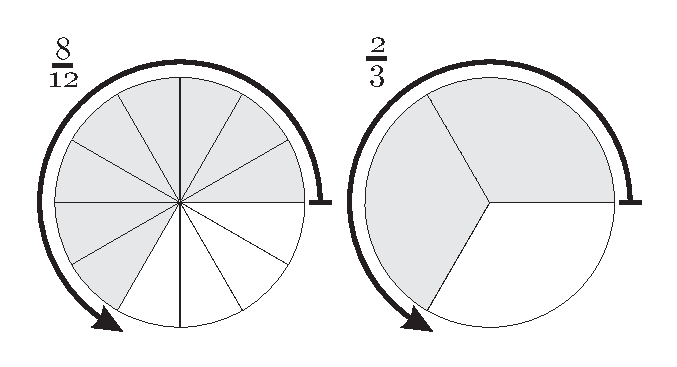
\includegraphics[width=4in]{ch1pizza.eps}
%\caption{$\frac{8}{12}$ of the pizza is the same as $\frac{2}{3}$ of the pizza.}
%\label{fig:mfoundation:pizza}
%\end{center}
%\end{figure}

You can also add rational numbers together by finding the \textit{lowest common denominator} and then adding the numerators. Finding a lowest common
denominator means finding the lowest number that both denominators are a
\textit{factor}\footnote{Some people say \textit{divisor} instead of factor.}
of. A factor of a number is an integer which evenly divides that number without
leaving a remainder. The following numbers all have a factor of 3
\begin{equation*}
3, 6, 9, 12, 15, 18, 21, 24,\ldots
\end{equation*}
and the following all have factors of 4
\begin{equation*}
4, 8, 12, 16, 20, 24, 28,\ldots
\end{equation*}
The common denominators between 3 and 4 are all the numbers that appear in both of these lists, like 12 and 24. The lowest common denominator of 3 and 4 is the smallest number that has both 3 and 4 as factors, which is 12.

For example, if we wish to add $\frac{3}{4} + \frac{2}{3}$, we first need to write both fractions so that their denominators are the same by finding the lowest common denominator, which we know is 12. We can do this by multiplying $\frac{3}{4}$ by $\frac{3}{3}$ and $\frac{2}{3}$ by $\frac{4}{4}$. $\frac{3}{3}$ and $\frac{4}{4}$ are really just complicated ways of writing $1$. Multiplying a number by $1$ doesn't change the number.
\begin{eqnarray}
\label{eq:mfoundation:r:lcd}
\frac 34 + \frac 23
&=&\frac 34\times\frac 33 + \frac 23\times\frac 44 \\ \nonumber
&=&\frac{3\times 3}{4\times 3} + \frac{2\times 4}{3\times 4} \\ \nonumber
&=&\frac 9{12} + \frac 8{12} \\ \nonumber
&=&\frac{9+8}{12} \\ \nonumber
&=&\frac{17}{12}
\end{eqnarray}

Dividing by a rational number is the same as multiplying by its reciprocal, as long as neither the numerator nor the denominator is zero:
\begin{equation}
\label{eq:mfoundation:r:div}
\frac ab \div \frac cd = \frac ab .\frac dc = \frac{ad}{bc}
\end{equation}

A rational number may be a \textit{proper} or \textit{improper} fraction. 

Proper fractions have a numerator that is smaller than the denominator. For example, 
\nequ{\frac{-1}{2}, \frac{3}{15}, \frac{-5}{-20}} are proper fractions.

Improper fractions have a numerator that is larger than the denominator. For example, \nequ{\frac{-10}{2}, \frac{15}{13}, \frac{-53}{-20}} are improper fractions. Improper fractions can always be written as the sum of an integer and a proper fraction.

\subsubsection{Converting Rationals into Decimal Numbers}
Converting rationals into decimal numbers is very easy. 

If you use a calculator, you can simply divide the numerator by the denominator.

If you do not have a calculator, then you have to use long division. 

Since long division was first taught in primary school, it will not be discussed here. If you have trouble with long division, then please ask your friends or your teacher to explain it to you.


\subsection{Irrational Numbers}
An \textit{irrational number} is any real number that is not a rational number. When expressed as decimals these numbers can never be fully written out as they have an infinite number of decimal places which never fall into a repeating pattern, for example $\sqrt{2} = 1,41421356\ldots$, $\pi = 3,14159265\ldots$. $\pi$ is a Greek letter and is pronounced ``pie''. 

\Exercise{Real Numbers}{
\begin{enumerate}
\item{Identify the number type (rational, irrational, real, integer) of each of the following numbers:}
\begin{enumerate}
\item{$\frac{c}{d}$ if $c$ is an integer and if $d$ is irrational.}
\item{$\frac{3}{2}$}
\item{-25}
\item{1,525}
\item{$\sqrt{10}$}
\end{enumerate}
\item{Is the following pair of numbers real and rational or real and irrational?
Explain.\\$\sqrt{4}$;$\frac{1}{8}$}					
\end{enumerate}
}

\section{Mathematical Symbols}

The following is a table of the meanings of some mathematical signs and symbols that you should have come across in earlier grades.

\begin{table}[htb]
\begin{center}
\begin{tabular}{|c|c|}\hline
Sign or Symbol & Meaning\\\hline\hline
$>$&greater than\\\hline
$<$&less than\\\hline
$\ge$& greater than or equal to\\\hline
$\le$& less than or equal to\\\hline
\end{tabular}
\end{center}
\end{table}

So if we write $x > 5$, we say that $x$ is greater than $5$ and if we write $x \geq y$, we mean that $x$ can be greater than or equal to $y$. Similarly, $<$ means `is less than' and $\leq$ means `is less than or equal to'. Instead of saying that $x$ is between $6$ and $10$, we often write $6<x<10$. This directly means `six is less than $x$ which in turn is less than ten'.

\Exercise{Mathematical Symbols}{
\begin{enumerate}
\item{Write the following in symbols:}
\begin{enumerate}
\item{$x$ is greater than 1}
\item{$y$ is less than or equal to $z$}
\item{$a$ is greater than or equal to 21}
\item{$p$ is greater than or equal to 21 and $p$ is less than or equal to 25}
\end{enumerate}
\end{enumerate}
}


\section{Infinity}
Infinity (symbol $\infty$) is usually thought of as something like ``the largest possible number" or ``the furthest possible distance". In mathematics, infinity is often treated as if it were a number, but it is clearly a very different type of ``number" than the integers or reals.

When talking about recurring decimals and irrational numbers, the term \textit{infinite} was used to describe \textit{never-ending} digits. 


\section{End of Chapter Exercises}
\begin{enumerate}
\item Calculate
\begin{enumerate}
\item $18-6\times 2$
\item $10+3(2+6)$
\item $50-10(4-2)+6$
\item $2\times 9-3(6-1)+1$
\item $8+24\div 4\times 2$
\item $30-3\times 4+2$
\item $36\div 4(5-2)+6$
\item $20-4\times 2+3$
\item $4+6(8+2)-3$
\item $100-10(2+3)+4$
\end{enumerate}
\item{If $p = q+4r$, then $r =.....$}
\item{Solve $\frac{x-2}{3} = x-3$}
\end{enumerate}

% CHILD SECTION END 



% CHILD SECTION START 

\chapter{Rational Numbers - Grade 10}
\label{m:n:rn:10}

\section{Introduction}
\label{m:n:rn:10:intro}

As described in Chapter~\ref{mfoundation}, a number is a way of representing quantity. The numbers that will be used in high school are all real numbers, but there are many different ways of writing any single real number.

This chapter describes \textit{rational numbers}.

\section{The Big Picture of Numbers}


\scalebox{1} % Change this value to rescale the drawing.
{
\begin{pspicture}(0,-4.764375)(14.481563,4.804375)
\psellipse[linewidth=0.04,dimen=outer](6.81,-0.484375)(6.81,4.28)
\psline[linewidth=0.04cm](8.18,3.695625)(8.26,-4.684375)
\psellipse[linewidth=0.04,dimen=outer](4.34,-1.364375)(3.8,2.5)
\psellipse[linewidth=0.04,dimen=outer](3.57,-1.854375)(2.57,1.61)
\usefont{T1}{ppl}{b}{n}
\rput(6.735781,4.350625){\Huge REAL $\mathbb{R}$}
\usefont{T1}{ppl}{b}{n}
\rput(11.03875,-0.484375){\Large Irrational $\mathbb{Q'}$}
\usefont{T1}{ppl}{b}{n}
\rput(5.11875,1.975625){\Large Rational $\mathbb{Q}$}
\usefont{T1}{ppl}{b}{n}
\rput(4.06875,0.275625){\Large Integers $\mathbb{Z}$}
\usefont{T1}{ppl}{b}{n}
\rput(3.21875,-2.324375){\Large Natural $\mathbb{N}$}
\psellipse[linewidth=0.04,dimen=outer](3.14,-2.354375)(1.68,0.83)
\usefont{T1}{ptm}{b}{n}
\rput(3.5735939,-1.024375){\Large Whole $\mathbb{N}_0$}
\end{pspicture} 
}


% \begin{center}
% \begin{pspicture}(-5,-3)(5,3)
% %\psgrid[gridcolor=gray]
% \psellipse(0,0)(5,3)
% \rput(0,2.4){Real Numbers}
% \psellipse(3,0)(1.5,2)
% \rput(3,0){Irrationals}
% \psellipse[fillcolor=lightgray,fillstyle=solid,linewidth=2pt](-2,0)(2.9,1.8)
% \rput(-2.8,1.4){Rationals}
% \psellipse(-1.5,0)(2.4,1.3)
% \rput(-2.2,0.9){Integers}
% \psellipse(-1,0)(1.9,0.8)
% \rput(-1.8,0.4){Whole}
% \psellipse(-0.5,0)(1.4,0.3)
% \rput(-0.5,0){Natural}
% \rput(-7,0){\parbox{3cm}{All numbers inside the grey oval are rational numbers.}}
% \end{pspicture}
% \end{center}

The term whole number does not have a consistent definition. Various authors use 
it in one different ways. We use the following definitions:
\begin{itemize}
\item natural numbers are (1, 2, 3, ...)
\item whole numbers are (0, 1, 2, 3, ...)
\item integers are (... -3, -2, -1, 0, 1, 2, 3, ....)
\end{itemize}


\section{Definition}

The following numbers are all rational numbers.
\begin{equation}
\frac{10}{1}, \quad \frac{21}{7}, \quad \frac{-1}{-3}, \quad \frac{10}{20}, \quad \frac{-3}{6}
\end{equation}
You can see that all the denominators and all the numerators are integers\footnote{Integers are the counting numbers (1, 2, 3, ...), their opposites (-1, -2, -3, ...), and 0.}.

\Definition{Rational Number}{A rational number is any number which can be written as:
\begin{equation}
\label{eq:mn:rational}
\frac{a}{b}
\end{equation}
where $a$ and $b$ are integers and $b\ne 0$.}

\Tip{Only fractions which have a numerator and a denominator (that is not 0) that are integers
are rational numbers.}

This means that all integers are rational numbers, because they can be written with a denominator of 1.

Therefore 
\begin{equation}
\frac{\sqrt{2}}{7}, \quad \frac{\pi}{20}
\end{equation}
are \textbf{not examples} of rational numbers, because in each case, either the numerator or the denominator is not an integer.

A number may not be written as an integer divided by another integer but may still
be a rational number. This is because the results might be able to be expressed
as an integer divided by an integer. The rule is if a number can be written
as fraction of integers it is rational, even if it can also be written in another
way as well. Here are two examples that might not look like rational numbers
at first glance but are because there are equivalent forms that are expressed as an
integer divided by another integer:

\begin{equation}
\quad \frac{-1,33}{-3} = \frac{133}{300}, \quad \frac{-3}{6,39} = \frac{-300}{639} = {-100}{213}
\end{equation}
are \textbf{not examples} of rational numbers, because in each case, either the numerator or the denominator is not an integer.


\Exercise{Rational Numbers}{
\begin{enumerate}
\item If $a$ is an integer, $b$ is an integer and $c$ is irrational, which of the following are rational numbers:
\begin{center}
\begin{tabular}{p{2cm}p{2cm}p{2cm}p{2cm}}
(i) $\frac{5}{6}$ & (ii) $\frac{a}{3}$ &(iii) $\frac{b}{2}$ & (iv) $\frac{1}{c}$\\
\end{tabular}
\end{center}
\item If $\frac{a}{1}$ is a rational number, which of the following are valid values for $a$?
\begin{center}
\begin{tabular}{p{2cm}p{2cm}p{2cm}p{2cm}}
(a) $1$ & (b) $-10$ & (c) $\sqrt{2}$ & (d) $2,1$\\
\end{tabular}
\end{center}
\end{enumerate}}

\section{Forms of Rational Numbers}
All integers and fractions with integer numerators and denominators are rational numbers. There are two more forms of rational numbers.

\Activity{Investigation}{Decimal Numbers}{You can write the rational number
$\frac{1}{2}$ as the decimal number 0,5. Write the following numbers as
decimals:
\begin{enumerate}
\item{$\frac{1}{4}$}
\item{$\frac{1}{10}$}
\item{$\frac{2}{5}$}
\item{$\frac{1}{100}$}
\item{$\frac{2}{3}$}
\end{enumerate}
Do the numbers after the decimal comma end or do they continue? If they continue, is there a repeating pattern to the numbers?}

You can write a rational number as a decimal number. Two types of decimal numbers can be written as rational numbers:
\begin{enumerate}
\item{decimal numbers that end or \textit{terminate}, for example the fraction $\frac{4}{10}$ can be written as 0,4.}
\item{decimal numbers that have a repeating pattern of numbers, for example the fraction $\frac{1}{3}$ can be written as $0,\dot{3}$.}
\end{enumerate}

For example, the rational number $\frac{5}{6}$ can be written in decimal notation as $0,8\dot{3}$, and similarly, the decimal number 0,25 can be written as a rational number as $\frac{1}{4}$.

\Tip{Notation for Repeating Decimals}{You can use a bar over the repeated numbers to indicate that the decimal is a repeating decimal.}

\section{Converting Terminating Decimals into Rational Numbers}
\label{mn:r:dr}
%\begin{syllabus}
%\item Identify rational numbers and convert between terminating or recurring decimals and the form: $\frac{a}{b}$;$a,b \in \mathbb{Z}$, $b\ne 0$
%\end{syllabus}

A decimal number has an integer part and a fractional part. For example, $10,589$ has an integer part of $10$ and a fractional part of $0,589$ because $10 + 0,589 = 10,589$. The fractional part can be written as a rational number, i.e., with a numerator and a denominator that are integers.

Each digit after the decimal point is a fraction with denominator in increasing powers of ten. For example:
\begin{itemize}
\item{$\frac {1}{10}$ is $0,1$}
\item{$\frac{1}{100}$ is $0,01$}
\end{itemize}
This means that:
\begin{eqnarray*}
2,103 &=& 2 + \frac 1{10} + \frac{0}{100} +\frac{3}{1000}\\
&=&2\frac{103}{1000}\\
&=&\frac{2103}{1000}\\
\end{eqnarray*}

\Exercise{Fractions}{
\begin{enumerate}
\item Write the following as fractions:
\begin{center}
\begin{tabular}{p{2cm}p{2cm}p{2cm}p{2cm}}
(a) $0,1$ & (b) $0,12$ & (c) $0,58$ & (d) $0,2589$\\
\end{tabular}
\end{center}
\end{enumerate}}

\section{Converting Repeating Decimals into Rational Numbers}
When the decimal is a repeating decimal, a bit more work is needed to write the fractional part of the decimal number as a fraction. We will explain by means of an example.

If we wish to write $0,\dot{3}$ in the form $\frac{a}{b}$ (where $a$ and $b$ are integers) then we would proceed as follows
\begin{eqnarray}
\label{eq:mn:r:dr:recur1:x}
x &=& 0,33333 \ldots \\
\label{eq:mn:r:dr:recur1:10x}
10x &=& 3,33333 \ldots \qquad
\text{multiply by 10 on both sides} \\ \nonumber
9x &=& 3\qquad\qquad\qquad
\text{subtracting \eqref{eq:mn:r:dr:recur1:x}
from \eqref{eq:mn:r:dr:recur1:10x}} \\ \nonumber
x &=& \frac 39 = \frac 13
\end{eqnarray}

And another example would be to write $5,\overline{432}$ as a rational fraction
\begin{eqnarray}
\label{eq:mn:r:dr:recur2:x}
x &=& 5,432432432 \ldots \\
\label{eq:mn:r:dr:recur2:1000x}
1000x &=& 5432,432432432 \ldots \qquad \text{multiply by 1000 on both sides} \\ \nonumber
\\ \nonumber
999x &=& 5427\quad\qquad\qquad
\text{subtracting \eqref{eq:mn:r:dr:recur2:x}
from \eqref{eq:mn:r:dr:recur2:1000x}}\\ \nonumber
x &=& \frac{5427}{999} = \frac{201}{37}
\end{eqnarray}

For the first example, the decimal number was multiplied by 10 and for the second example, the decimal number was multiplied by 1000. This is because for the first example there was only one number (i.e. 3) that recurred, while for the second example there were three numbers (i.e. 432) that recurred.

In general, if you have one number recurring, then multiply by 10, if you have two numbers recurring, then multiply by 100, if you have three numbers recurring, then multiply by 1000. Can you spot the pattern yet?

The number of zeros after the 1 is the same as the number of recurring numbers.

But not all decimal numbers can be written as rational numbers, because some decimal numbers like $\sqrt{2}=1,4142135...$ are irrational numbers and cannot be written with an integer numerator and an integer denominator. However, when possible, you should try to use rational numbers or fractions instead of decimals.

\Exercise{Repeated Decimal Notation}{
\begin{enumerate}
\item Write the following using the repeated decimal notation:
\begin{enumerate}
\item $0,11111111\ldots$
\item $0,1212121212\ldots$
\item $0,123123123123\ldots$
\item $0,11414541454145\ldots$
\end{enumerate}
\item Write the following in decimal form, using the repeated decimal notation:
\begin{enumerate}
\item $\frac{2}{3}$
\item $1\frac{3}{11}$
\item $4\frac{5}{6}$
\item $2\frac{1}{9}$
\end{enumerate}
\item Write the following decimals in fractional form:
\begin{enumerate}
\item $0,633\dot{3}$
\item $5,3131\overline{31}$
\item $0,99999\dot{9}$
\end{enumerate}
\end{enumerate}}

\section{Summary}
The following are rational numbers:
\begin{itemize}
\item Fractions with both denominator and numerator as integers.
\item Integers.
\item Decimal numbers that end.
\item Decimal numbers that repeat.
\end{itemize}

\section{End of Chapter Exercises}
\begin{enumerate}
\item If $a$ is an integer, $b$ is an integer and $c$ is irrational, which of the following are rational numbers:
\begin{enumerate}
\item $\frac{5}{6}$
\item $\frac{a}{3}$
\item $\frac{b}{2}$
\item $\frac{1}{c}$
\end{enumerate}
\item Write each decimal as a simple fraction:
\begin{enumerate}
\item $0,5$
\item $0,12$
\item $0,6$
\item $1,59$
\item $12,27\dot{7}$
\end{enumerate}
\item Show that the decimal $3,2\dot1\dot8$ is a rational number.
\item Showing all working, express $0,7\dot8$ as a fraction $\frac{a}{b}$ where $a, b \in \mathbb Z$.
\end{enumerate}

% CHILD SECTION END 



% CHILD SECTION START 

\chapter{Exponentials - Grade 10}
\label{m:n:en:10}


\section{Introduction}
\label{mn:intro}

In this chapter, you will learn about the short-cuts to writing $2\times 2\times 2 \times 2$. This is known as writing a number in \textit{exponential notation}.

\section{Definition}
\label{m:n:en:10:def}

Exponential notation is a short way of writing the same number multiplied by
itself many times. For example, instead of $5 \times 5 \times 5$, we write $5^3$ to show that the number 5 is multiplied by itself 3 times and we say ``5 to the power of 3''. Likewise $5^2$ is $5\times 5$ and $3^5$ is $3\times 3\times 3\times 3\times 3$. We will now have a closer look at writing numbers using exponential notation.

\Definition{Exponential Notation}{Exponential notation means a number written like 
\nequ{a^n}
when $n$ is an integer and $a$ can be any real number. $a$ is called the \textit{base} and $n$ is called the \textit{exponent} or \textit{index}.}

The $n$th power of $a$ is defined as:
\begin{equation}
\label{eq:mn:e:nth}
a^n=a\times a\times\cdots\times a\qquad\textrm{(}n\textrm{ times)}
\end{equation}
with $a$ multiplied by itself $n$ times.

We can also define what it means if we have a negative exponent, $-n$. Then, 
\begin{equation}
\label{eq:mn:e:nth:neg}
a^{-n}=\frac{1}{a\times a\times\cdots\times a\qquad\textrm{(}n\textrm{ times)}}
\end{equation}

\Tip{Exponentials}{If $n$ is an even integer, then $a^n$ will always be positive for any non-zero real number $a$. For example, although $-2$ is negative, $(-2)^2=-2\times-2=4$ is positive and so is $(-2)^{-2}=\frac{1}{-2\times-2}=\frac 14$.}

\section{Laws of Exponents}
%\begin{syllabus}
%\item Simplify expressions using the laws of exponents for integral exponents.
%\end{syllabus}

There are several laws we can use to make working with exponential numbers easier. Some of these laws might have been seen in earlier grades, but we will list all the laws here for easy reference and explain each law in detail, so that you can understand them, and not only remember them.

\begin{eqnarray}
\label{eq:mn:e:law1}
a^0 &=& 1\\
\label{eq:mn:e:law2}
a^m \times a^n &=& a^{m+n} \\
\label{eq:mn:e:law3}
a^{-n} &=& \frac{1}{a^{n}}\\
\label{eq:mn:e:law4}
a^m \div a^n &=& a^{m-n} \\
\label{eq:mn:e:law5}
(ab)^n &=& a^nb^n \\
\label{eq:mn:e:law6}
(a^m)^n &=& a^{mn}
\end{eqnarray}

\subsection{Exponential Law 1: $a^0=1$}
Our definition of exponential notation shows that
\begin{eqnarray}
\label{eq:mn:e:law1:proof}
a^0 &=& 1\quad ,\quad (a \neq 0)
\end{eqnarray} 

For example, $x^0=1$ and $(1\;000\;000)^0=1$.

\Exercise{Application using Exponential Law 1: $a^0=1,  (a\neq 0)$}{
\begin{enumerate}
\item{$16^0 = 1$}\\
\item{$16a^0 = 16$}\\
\item{$(16 + a)^0 = 1$}\\
\item{$(-16)^0 = 1$}\\
\item{$-16^0 = -1$}\\
\end{enumerate}}


\subsection{Exponential Law 2: $a^m \times a^n=a^{m+n}$}
Our definition of exponential notation shows that
\begin{eqnarray}
\label{eq:mn:e:law2:proof}
a^m \times a^n &=& 1\times a\times\ldots\times a\qquad\textrm{(}m\textrm{
times)}\\\nonumber
&&\!\!\!\!\times 1\times a\times\ldots\times a\qquad\textrm{(}n\textrm{
times)}\\\nonumber
&=& 1\times a\times\ldots\times a\qquad\textrm{(}m+n\textrm{
times)}\\\nonumber
&=& a^{m+n}
\end{eqnarray}

For example,
\begin{eqnarray*}
2^7\times2^3&=&(2\times 2\times 2\times 2\times 2\times 2\times 2)\times(2\times 2\times 2)\\
&=&2^{7+3}\\
&=&2^{10}
\end{eqnarray*}

\begin{IFact}
{This simple law is the reason why exponentials were originally invented. In the days before calculators, all multiplication had to be done by hand with a pencil and a pad of paper. Multiplication takes a very long time to do and is very tedious. Adding numbers however, is very easy and quick to do. If you look at what this law is saying you will realise that it means that adding the exponents of two exponential numbers (of the same base) is the same as multiplying the two numbers together. This meant that for certain numbers, there was no need to actually multiply the numbers together in order to find out what their multiple was. This saved mathematicians a lot of time, which they could use to do something more productive.}
\end{IFact}

\Exercise{Application using Exponential Law 2: $a^m \times a^n=a^{m+n}$}{
\begin{enumerate}
\item{$x^2 \cdot x^5=x^7$}\\
%\item{$2x^3y\times 5x^2y^7=10x^5y^8$}\\
\item{$2^3.2^4=2^7$} \textit{[Take note that the base ($2$) stays the same.]}\\
\item{$3\times 3^{2a}\times 3^2 = 3^{2a+3}$}
\end{enumerate}}

\subsection{Exponential Law 3: $a^{-n}=\frac{1}{a^{n}},\quad a\neq 0 $}
Our definition of exponential notation for a negative exponent shows that
\begin{eqnarray}
\label{eq:mn:e:law3:proof}
a^{-n}&=&1\div a\div\ldots\div a\qquad\textrm{(}n
\textrm{ times)}\\\nonumber
&=&\frac 1{1\times a\times\dots\times a}\qquad\textrm{(}n
\textrm{ times)}\\\nonumber
&=&\frac 1{a^n}
\end{eqnarray}
This means that a minus sign in the exponent is just another way of showing that the whole exponential number is to be divided instead of multiplied.

For example,
\begin{eqnarray*}
2^{-7}&=&\frac{1}{2\times 2\times 2\times 2\times 2\times 2\times 2}\\
&=&\frac{1}{2^{7}}
\end{eqnarray*}

\Exercise{Application using Exponential Law 3: $a^{-n}=\frac{1}{a^{n}}, a \neq0$}{
\begin{enumerate}
\item{$2^{-2}=\frac{1}{2^2}=\frac{1}{4}$}
\item{$\frac{2^{-2}}{3^2}=\frac{1}{2^2.3^2}=\frac{1}{36}$}
\item{$(\frac{2}{3})^{-3}=(\frac{3}{2})^{3}=\frac{27}{8}$}
\item{$\frac{m}{n^{-4}}=mn^4$}
\item{$\frac{a^{-3}\cdot x^4}{a^5\cdot x^{-2}}=\frac{x^4\cdot x^2}{a^3\cdot a^5}=\frac{x^6}{a^8}$}
\end{enumerate}}

\subsection{Exponential Law 4: $a^m \div a^n=a^{m-n}$}
We already realised with law 3 that a minus sign is another way of saying that the exponential number is to be divided instead of multiplied. Law 4 is just a more general way of saying the same thing. We get this law by  multiplying law 3 by $a^m$ on both sides and using law 2.
\begin{eqnarray}
\label{eq:mn:e:law4:proof}
\frac {a^m}{a^n}&=&a^ma^{-n}\\\nonumber
&=&a^{m-n}
\end{eqnarray}

For example,
\begin{eqnarray*}
2^7 \div 2^3&=&\frac{2\times 2\times 2\times 2\times 2\times 2\times 2}{2\times 2\times 2}\\
&=&2\times 2\times 2\times 2\\
&=&2^{4}\\
&=&2^{7-3}
\end{eqnarray*}

\Exercise{Exponential Law 4: $a^m \div a^n=a^{m-n}$}{
\begin{enumerate}
\item{$\frac{a^6}{a^2}= a^{6-2}= a^4$}
\item{$\frac{3^2}{3^6}=3^{2-6}=3^{-4}=\frac{1}{3^4}$}\textit{[Always give final answer with positive index]}
\item{$\frac{32a^2}{4a^8}=8a^{-6}=\frac{8}{a^6}$}
\item{$\frac{a^{3x}}{a^4}=a^{3x-4}$}
\end{enumerate}
}

\subsection{Exponential Law 5: $(ab)^n=a^nb^n$}
The order in which two real numbers are multiplied together does not matter. Therefore,
\begin{eqnarray}
\label{eq:mn:e:law5:proof}
(ab)^n &=& a\times b\times a\times b\times\ldots\times
a\times b \qquad\textrm{(}n\textrm{ times)}\\\nonumber
&=& a\times a\times\ldots\times a\qquad\textrm{(}n\textrm{ times)}\\\nonumber
&&\!\!\!\!\times b\times b\times\ldots\times b \qquad\textrm{(}n\textrm{ times)}\\\nonumber
&=& a^nb^n
\end{eqnarray}

For example,
\begin{eqnarray*}
(2\cdot 3)^4 &=&(2\cdot 3)\times(2\cdot 3)\times(2\cdot 3)\times(2\cdot 3)\\
&=&(2 \times 2 \times 2 \times 2)\times(3 \times 3 \times 3 \times 3)\\
&=&(2^4)\times(3^4)\\
&=&2^4 3^4
\end{eqnarray*}

\Exercise{Exponential Law 5: $(ab)^n=a^nb^n$}{
\begin{enumerate}
\item{$(2xy)^3=2^3x^{3}y^3=8x^3y^3$}
\item{$(\frac{7a}{b})^2=\frac{49a^2}{b^2}$}
\item{$(5a)^3=125a^{3}$}
\end{enumerate}
}

\subsection{Exponential Law 6: $(a^m)^n=a^{mn}$}
We can find the exponential of an exponential just as easily as we can for a number. After all, an exponential number is a real number.
\begin{eqnarray}
\label{eq:mn:e:law6:proof}
(a^m)^n &=& a^m\times a^m\times\ldots\times a^m\qquad\textrm{(}n\textrm{ times)}\\\nonumber
&=& a\times a\times\ldots\times a\qquad\textrm{(}m\times n\textrm{ times)}\\\nonumber
&=& a^{mn}
\end{eqnarray}

For example,
\begin{eqnarray*}
(2^2)^3 &=&(2^2)\times(2^2)\times(2^2)\\
&=&(2 \times 2)\times(2 \times 2)\times(2 \times 2)\\
&=&(2^6)\\
&=&2^{(2\times3)}
\end{eqnarray*}

\Exercise{Exponential Law 6: $(a^m)^n=a^{mn}$}{
\begin{enumerate}
 \item{$(x^3)^4=x^{12}$}
 \item{$[(a^4)^3]^2=a^{24}$}
 \item{$(3^{n+3})^2=3^{2n+6}$}
\end{enumerate}}

\begin{wex}{Simplifying indices}
 {Simplify: $\frac{5^{2x-1}\cdot 9^{x-2}}{15^{2x-3}}$}
 {
  \westep{Factorise all bases into prime factors:}
  \begin{eqnarray*}
   &=&\frac{5^{2x-1}\cdot (3^2)^{x-2}}{(5.3)^{2x-3}}\quad\quad\quad\\
   &=&\frac{5^{2x-1}\cdot 3^{2x-4}}{5^{2x-3}\cdot 3^{2x-3}}
  \end{eqnarray*}
  \westep{Add and subtract the indices of the same bases as per laws 2 and 4:}
  \begin{eqnarray*}
   &=&5^{2x-1-2x+3}\cdot 3^{2x-4-2x+3}\\
   &=&5^2\cdot 3^{-1}
  \end{eqnarray*}
  \westep{Write simplified answer with positive indices:}
  \begin{equation*}
   =\frac{25}{3}\quad\quad\quad\quad\quad\quad\quad\quad
  \end{equation*}
 }
\end{wex}

\Activity{Investigation}{Exponential Numbers}{
Match the answers to the questions, by filling in the correct answer into the \textbf{Answer} column.
Possible answers are: $\frac{3}{2}$, $1$, $-1$, $-\frac{1}{3}$, $8$. Answers may be repeated.

\begin{center}
\begin{tabular}{|c|c|}\hline\hline
\textbf{Question} & \textbf{Answer}\\\hline\hline
$2^3$&\\\hline
$7^{3-3}$&\\\hline
$(\frac{2}{3})^{-1}$&\\\hline
$8^{7-6}$&\\\hline
$(-3)^{-1}$&\\\hline
$(-1)^{23}$&\\\hline\hline
\end{tabular}
\end{center}}

\section{End of Chapter Exercises}
\begin{enumerate}
 \item{Simplify as far as possible:
  \begin{center}
   \begin{tabular}{p{2cm}p{2cm}p{2cm}p{8cm}}
    (a) $302^0$ & (b) $1^0$ & (c) $(xyz)^0$ & (d) $[(3x^4y^7z^{12})^5 (-5x^9y^3z^4)^2]^0$\\
    (e) $(2x)^3$ & (f) $(-2x)^3$ & (g) $(2x)^4$ & (h) $(-2x)^4$\\
   \end{tabular}
  \end{center}
 }
 \item{{Simplify without using a calculator. Leave your answers with positive exponents.}
  \begin{enumerate}
   \item $\frac{3x^{-3}}{(3x)^2}$\\
   \item $5x^0+8^{-2}-{(\frac{1}{2})^{-2}}\cdot 1^x$\\
   \item $\frac{5^{b-3}}{5^{b+1}}$\\
  \end{enumerate}
 }
 \item{Simplify, showing all steps:
  \begin{enumerate}
   \item $\frac{2^{a-2}.3^{a+3}}{6^a}$\\
   \item $\frac{a^{2m+n+p}}{a^{m+n+p} \cdot a^m}$\\
   \item $\frac{3^n \cdot 9^{n-3}}{27^{n-1}}$\\
   \item $(\frac{2x^{2a}}{y^{-b}})^{3}$\\
   \item $\frac{2^{3x-1} \cdot 8^{x+1}}{4^{2x-2}}$\\
   \item $\frac{6^{2x} \cdot 11^{2x}}{22^{2x-1} \cdot 3^{2x}}$\\
  \end{enumerate}
 }
 \item{Simplify, without using a calculator:
  \begin{enumerate}
   \item $\frac{(-3)^{-3} \cdot (-3)^2}{(-3)^{-4}}$\\
   \item ${(3^{-1} + 2^{-1})^{-1}}$\\
   \item $\frac{9^{n-1} \cdot 27^{3-2n}}{81^{2-n}}$\\
   \item $\frac{2^{3n+2} \cdot 8^{n-3}}{4^{3n-2}}$\\
  \end{enumerate}
 }
\end{enumerate}





% too advanced for gr 10
%\item{Show that
%\nequ{\left(\frac{a}{b}\right)^n=\frac{a^n}{b^n}}}
%\item{Show, using Equation~\ref{eq:mn:e:nth}, that
%\item{[SC 2005/03 SG1] Simplify, without use of a calculator:
%\nequ{(3^{-1}+2^{-1})^{-1}}}
%\item{[SC 2005/03 SG1] Simplify, without use of a calculator:
%\nequ{\frac{9^{n-1}\cdot 27^{3-2n}}{81^{2-n}}}}
%\item{[SC 2004/11 SG1] Simplify, without use of a calculator:
%\nequ{\frac{2^{3n+2}\cdot 8^{n-3}}{4^{3n-2}}}}
%\item{[SC 2003/11 HG1] Simplify, without using a calculator:
%\nequ{\frac{5^{a-2}\cdot2^{a+2}}{10^a-10^{a-1}\cdot 2}}}
%\item{[SC 2002/11 SG1] Simplify completely:
%\nequ{\frac{2\cdot 3^x - 3 ^{x-1}}{5\cdot 3^x}}}
%\item{[SC 2003/11 SG1] Simplify completely:
%\nequ{\frac{3^{n+1}-3^n}{3^{n-1}}}}
%\item{[SC 2005/11 SG1] Simplify completely:
%\nequ{
%\frac{6^{2x-1}-36^x}{6^{2x}}}}
%\item{[IEB, Nov. 2002, HG] Simplify fully: \qquad $\dfrac{4^x + 3 . 2^{ 2x-1}}{2^{-x} . 2^{ 3x+2}}$}
%\item{\nts{More end of chapter exercises involving the simplification of expressions using the laws of exponents for integral exponents are needed.}}
%\end{enumerate}

%\section{End of Chapter Exercises}
%\begin{enumerate}
%\item{Show that
%\nequ{\left(\frac{a}{b}\right)^n=\frac{a^n}{b^n}}}
%\item{Show, using Equation~\ref{eq:mn:e:nth}, that
%\nequ{a^1=a}}
%\item{Simplify as far as possible:
%\begin{center}
%\begin{tabular}{p{2cm}p{2cm}p{2cm}p{5cm}}
%(a) $302^0$ & (b) $1^0$ & (c) $(xyz)^0$ & (d) $[(3x^4y^7z^{12})^5 (-5x^9y^3z^4)^2]^0$\\
%(e) $(2x)^3$ & (f) $(-2x)^3$ & (g) $(2x)^4$ & (h) $(-2x)^4$\\
%\end{tabular}
%\end{center}}
%\item{[SC 2005/03 SG1] Simplify, without use of a calculator:
%\nequ{(3^{-1}+2^{-1})^{-1}}}
%\item{[SC 2005/03 SG1] Simplify, without use of a calculator:
%\nequ{\frac{9^{n-1}\cdot 27^{3-2n}}{81^{2-n}}}}
%\item{[SC 2004/11 SG1] Simplify, without use of a calculator:
%\nequ{\frac{2^{3n+2}\cdot 8^{n-3}}{4^{3n-2}}}}
%\item{[SC 2003/11 HG1] Simplify, without using a calculator:
%\nequ{\frac{5^{a-2}\cdot2^{a+2}}{10^a-10^{a-1}\cdot 2}}}
%\item{[SC 2002/11 SG1] Simplify completely:
%\nequ{\frac{2\cdot 3^x - 3 ^{x-1}}{5\cdot 3^x}}}
%\item{[SC 2003/11 SG1] Simplify completely:
%\nequ{\frac{3^{n+1}-3^n}{3^{n-1}}}}
%\item{[SC 2005/11 SG1] Simplify completely:
%\nequ{
%\frac{6^{2x-1}-36^x}{6^{2x}}}}
%\item{[IEB, Nov. 2002, HG] Simplify fully: \qquad $\dfrac{4^x + 3 . 2^{ 2x-1}}{2^{-x} . 2^{ 3x+2}}$}
%\item{\nts{More end of chapter exercises involving the simplification of expressions using the laws of exponents for integral exponents are needed.}}
%\end{enumerate}

% CHILD SECTION END 



% CHILD SECTION START 

\chapter{Estimating Surds - Grade 10}
\label{m:n:s:10}

\section{Introduction}

%\begin{syllabus}
%\item Establish between which two integers any simple surd lies.
%\end{syllabus}

You should know by now what the $n$th root of a number means. If the $n$th root of a number cannot be simplified to a rational number, we call it a $\textit{surd}$. For example, $\sqrt{2}$ and $\sqrt[3]{6}$ are surds, but $\sqrt{4}$ is not a surd because it can be simplified to the rational number 2. 

In this chapter we will only look at surds that look like $\sqrt[n]{a}$, where $a$ is any positive number, for example $\sqrt{7}$ or $\sqrt[3]{5}$. It is very common for $n$ to be $2$, so we usually do not write $\sqrt[2]{a}$. Instead we write the surd as just $\sqrt{a}$, which is much easier to read.

It is sometimes useful to know the approximate value of a surd without having to use a calculator. For example, we want to be able to estimate where a surd like $\sqrt{3}$ is on the number line. So how do we know where surds lie on the number line? From a calculator we know that $\sqrt{3}$ is equal to $1,73205...$. It is easy to see that $\sqrt{3}$ is above 1 and below 2. But to see this for other surds like $\sqrt{18}$ without using a calculator, you must first understand the following fact:

\begin{IFact}{
If $a$ and $b$ are positive whole numbers, and $a < b$, then $\sqrt[n]{a} < \sqrt[n]{b}$. (Challenge: Can you explain why?) 
}\end{IFact}

If you don't believe this fact, check it for a few numbers to convince yourself it is true.

How do we use this fact to help us guess what $\sqrt{18}$ is? Well, you can easily see that $18 < 25$? Using our rule, we also know that $\sqrt{18} < \sqrt{25}$. But we know that $5^2 = 25$ so that $\sqrt{25} = 5$. Now it is easy to simplify to get $\sqrt{18} < 5$. Now we have a better idea of what $\sqrt{18}$ is. 

Now we know that $\sqrt{18}$ is less than 5, but this is only half the story. We can use the same trick again, but this time with 18 on the right-hand side. You will agree that $16 < 18$. Using our rule again, we also know that $\sqrt{16} < \sqrt{18}$. But we know that 16 is a perfect square, so we can simplify $\sqrt{16}$ to $4$, and so we get $4 < \sqrt{18}$! 

Can you see now that we now have shown that $\sqrt{18}$ is between 4 and 5? If we check on our calculator, we can see that $\sqrt{18} = 4,1231...$, and we see that our idea was right! You will notice that our idea used perfect squares that were close to the number 18. We found the closest perfect square underneath 18, which was $4^2 = 16$, and the closest perfect square above 18, which was $5^2 = 25$. Here is a quick summary of what a perfect square or cube is: 

\begin{IFact}{A perfect square is the number obtained when an integer is squared. For example, 9 is a perfect square since $3^2=9$. Similarly, a perfect cube is a number which is the cube of an integer. For example, 27 is a perfect cube, because $3^3=27$.}\end{IFact}

To make it easier to use our idea, we will create a list of some of the perfect squares and perfect cubes. The list is shown in Table~\ref{tab:mn:s:perfectsquarecube}.

\begin{table}[htbp]
\begin{center}
\caption{Some perfect squares and perfect cubes}
\label{tab:mn:s:perfectsquarecube}
\begin{tabular}{|c|c|c|}\hline
Integer & Perfect Square & Perfect Cube\\\hline\hline
0&0&0\\\hline
1&1&1\\\hline
2&4&8\\\hline
3&9&27\\\hline
4&16&64\\\hline
5&25&125\\\hline
6&36&216\\\hline
7&49&343\\\hline
8&64&512\\\hline
9&81&729\\\hline
10&100&1000\\\hline
\end{tabular}
\end{center}
\end{table}

When given the surd $\sqrt[3]{52}$ you should be able to tell that it lies somewhere between 3 and 4, because $\sqrt[3]{27}=3$ and $\sqrt[3]{64}=4$ and 52 is between 27 and 64. In fact $\sqrt[3]{52}=3,73\ldots$ which is indeed between 3 and 4.

\section{Drawing Surds on the Number Line (Optional)}
How can we accurately draw a surd like $\sqrt{5}$ on the number line? Well, we \emph{could} use a calculator to find $\sqrt{5} = 2,2360...$ and measure the distance along the number line using a ruler. But for some surds, there is a much easier way. 

Let us call the surd we are working with $\sqrt{x}$. Sometimes, we can write $x$ as the sum of two perfect squares, so $x = b^2 + c^2$. We know from Pythagoras' theorem that $a^2 = b^2 + c^2$, in this case $a=\sqrt{x}$. In other words $\sqrt{x} = \sqrt{b^2 + c^2}$, where $\sqrt{x}$ is the length of the hypotenuse of a triangle that has sides that have lengths of b and c. Now if we draw a triangle with $b$ on the number line and $c$ perpendicular to the number line, we can use a compass to draw a circle from the top of side $c$ down to the number line. The intersection of the circle with the number line will be the point $\sqrt{x}$! 

% Generated with LaTeXDraw 2.0.5
% Thu Sep 02 13:20:21 SAST 2010
% \usepackage[usenames,dvipsnames]{pstricks}
% \usepackage{epsfig}
% \usepackage{pst-grad} % For gradients
% \usepackage{pst-plot} % For axes
\scalebox{1} % Change this value to rescale the drawing.
{
\begin{pspicture}(0,-1.1858333)(8.42,4.48)
\rput(3.42,-0.52){\psaxes[linewidth=0.04,ticksize=0.10583333cm](0,0)(0,0)(5,5)}
\psline[linewidth=0.04cm](3.4,-0.54)(7.4,2.46)
\psline[linewidth=0.04cm](7.4,2.46)(7.42,-0.5)
\psline[linewidth=0.04cm](7.04,-0.12)(7.42,-0.12)
\psline[linewidth=0.04cm](7.06,-0.1)(7.06,-0.54)
\psarc[linewidth=0.04,linestyle=dashed,dash=0.16cm 0.16cm](4.2,-0.28){4.2}{355.46222}{40.992195}
\usefont{T1}{ptm}{m}{n}
\rput(5.835625,0.065){4}
\usefont{T1}{ptm}{m}{n}
\rput(7.746406,1.005){3}
\end{pspicture} 
}



\begin{IFact}{Not all numbers can be written as the sum of two squares. See if you can find a pattern of the numbers that can.}\end{IFact}


\begin{wex}{Estimating Surds}
{Find the two consecutive integers such that $\sqrt{26}$ lies between them.\\(Remember that consecutive numbers are two numbers one after the other, like 5 and 6 or 8 and 9.)}{
\westep{From the table find the largest perfect square below 26} This is $5^2 = 25$. Therefore $5 < \sqrt{26}$. 
\westep{From the table find smallest perfect square above 26} This is $6^2 = 36$. Therefore $\sqrt{26} < 6$. 
\westep{Put the inequalities together} Our answer is $5 < \sqrt{26} < 6$.}
\end{wex}

\begin{wex}{Estimating Surds}
{$\sqrt[3]{49}$ lies between:
\begin{tabular}{llll}
(a) 1 and 2 &  (b) 2 and 3 &  (c) 3 and 4 &  (d) 4 and 5\\
\end{tabular}}{
\westep{Consider (a) as the solution} If $1 < \sqrt[3]{49} < 2$ then cubing all terms gives $1 < 49 < 2^3$. Simplifying gives $1 < 49 < 8$ which is false. So $\sqrt[3]{49}$ does not lie between 1 and 2.
\westep{Consider (b) as the solution} If $2 < \sqrt[3]{49} < 3$ then cubing all terms gives $2^3 < 49 < 3^3$. Simplifying gives $8 < 49 < 27$ which is false. So $\sqrt[3]{49}$ does not lie between 2 and 3. 
\westep{Consider (c) as the solution} If $3 < \sqrt[3]{49} < 4$ then cubing all terms gives $3^3 < 49 < 4^3$. Simplifying gives $27 < 49 < 64$ which is true. So $\sqrt[3]{49}$ lies between 3 and 4. 
}
\end{wex}

\section{End of Chapter Exercises}
\begin{tabular}{clllll}
1. & $\sqrt{5}$ lies between &
(a) 1 and 2 &  (b) 2 and 3 &  (c) 3 and 4 &  (d) 4 and 5\\
2. & $\sqrt{10}$ lies between &
(a) 1 and 2 & (b) 2 and 3 & (c) 3 and 4 & (d) 4 and 5\\
3. & $\sqrt{20}$ lies between&
(a) 2 and 3 & (b) 3 and 4 & (c) 4 and 5 &	(d) 5 and 6\\
4. & $\sqrt{30}$ lies between &
(a) 3 and 4 &(b) 4 and 5 & (c) 5 and 6 & (d) 6 and 7\\
5. & $\sqrt[3]{5}$ lies between &
(a) 1 and 2 &  (b) 2 and 3 &  (c) 3 and 4 &  (d) 4 and 5\\
6. & $\sqrt[3]{10}$ lies between &
(a) 1 and 2 &(b) 2 and 3 & (c) 3 and 4 & (d) 4 and 5\\
7. & $\sqrt[3]{20}$ lies between &
(a) 2 and 3 &(b) 3 and 4 &(c) 4 and 5 & (d) 5 and 6\\
8. & $\sqrt[3]{30}$ lies between &
(a) 3 and 4 &(b) 4 and 5 & (c) 5 and 6 &(d) 6 and 7
\end{tabular}


% CHILD SECTION END 



% CHILD SECTION START 

\chapter{Irrational Numbers and Rounding Off - Grade 10}
\label{m:n:re:10}

%\begin{syllabus}
%\item Round rational and irrational numbers to an appropriate degree of accuracy.
%\end{syllabus}

\section{Introduction}
You have seen that repeating decimals may take a lot of paper and ink to write out. Not only is that impossible, but writing numbers out to many decimal places or \textit{a high accuracy} is very inconvenient and rarely gives practical answers. For this reason we often estimate the number to a certain number of decimal places or to a given number of \textit{significant figures}, which is even better.

\section{Irrational Numbers}

Irrational numbers are numbers that cannot be written as a rational number. You should know that a rational number can be written as a fraction with the numerator and denominator as integers. This means that any number that is \textit{not} a terminating decimal number or a repeating decimal number is irrational. Examples of irrational numbers are:
\begin{eqnarray*}
\sqrt{2},\quad\sqrt{3},\quad\sqrt[3]{4},\quad
\pi,\\
\frac{1 + \sqrt{5}}{2}\approx 1,618\,033\,989\,
\end{eqnarray*}

\Tip{When irrational numbers are written in decimal form, they go on forever and
there is no repeated pattern of digits.}

\Tip{Irrational Numbers}{If you are asked to identify whether a number is rational or irrational, first write the number in decimal form. If the number is terminated then it is rational. If it goes on forever, then look for a repeated pattern of digits. If there is no repeated pattern, then the number is irrational.}

When you write irrational numbers in decimal form, you may (if you have a lot of time and paper!) continue writing them for many, many decimal places. However, this is not convenient and it is often necessary to round off.

\Activity{Investigation}{Irrational Numbers}{Which of the following cannot be
written as a rational number? 

\textbf{Remember}: A rational number is a fraction with numerator and denominator as integers. Terminating decimal numbers or repeating decimal numbers are rational.
\vspace{0.5cm}
\begin{enumerate}
\item{$\pi=3,1415926535 89793 23846 26433 83279 50288 41971 69399 37510\ldots$}
\item{1,4}
\item{$1,618\,033\,989\,\ldots$}
\item{100}
\end{enumerate}}

\section{Rounding Off}

Rounding off or approximating a decimal number to a given number of decimal places is the quickest way to approximate a number. For example, if you wanted to round-off $2,6525272$ to three decimal places then you would first count three places after the decimal.
\nequ{2,652|5272}
All numbers to the right of $|$ are ignored after you determine whether the number in the third decimal place must be rounded up or rounded down. You \textit{round up} the final digit if the first digit after the $|$ was greater or equal to 5 and \textit{round down} (leave the digit alone) otherwise. In the case that the first digit before the $|$ is 9 \textit{and} the you need to round up the 9 becomes a 0 and the second digit before the $|$ is rounded up.

So, since the first digit after the $|$ is a 5, we must round up the digit in the third decimal place to a 3 and the final answer of $2,6525272$ rounded to three decimal places is
\nequ{2,653}

\begin{wex}{Rounding-Off}{Round-off the following numbers to the indicated number of decimal places:
\begin{enumerate}
\item{$\frac{120}{99}=1,212121212\Dot{1}\Dot{2}$ to 3 decimal places}
\item{$\pi=3,141592654\ldots$ to 4 decimal places}
\item{$\sqrt{3}=1,7320508\ldots$ to 4 decimal places}
\end{enumerate}}{\westep{Determine the last digit that is kept and mark the cut-off point with $|$.}
\begin{enumerate}
\item{$\frac{120}{99}=1,212|121212\Dot{1}\Dot{2}$}
\item{$\pi=3,1415|92654\ldots$}
\item{$\sqrt{3}=1,7320|508\ldots$}
\end{enumerate}
\westep{Determine whether the last digit is rounded up or down.}
\begin{enumerate}
\item{The last digit of $\frac{120}{99}=1,212|121212\Dot{1}\Dot{2}$ must be rounded-down.}
\item{The last digit of $\pi=3,1415|92654\ldots$ must be rounded-up.}
\item{The last digit of $\sqrt{3}=1,7320|508\ldots$ must be rounded-up.}
\end{enumerate}
\westep{Write the final answer.}
\begin{enumerate}
\item{$\frac{120}{99}=1,212$ rounded to 3 decimal places}
\item{$\pi=3,1416$ rounded to 4 decimal places}
\item{$\sqrt{3}=1,7321$ rounded to 4 decimal places}
\end{enumerate}}
\end{wex}

\section{End of Chapter Exercises}
\begin{enumerate}
\item{Write the following rational numbers to 2 decimal places:
\begin{enumerate}
\item{$\frac{1}{2}$}
\item{$1$}
\item{$0,11111\overline{1}$}
\item{$0,99999\overline{1}$}
\end{enumerate}
}
\item{Write the following irrational numbers to 2 decimal places:
\begin{enumerate}
\item{$3,141592654\ldots$}
\item{$1,618\,033\,989\,\ldots$}
\item{$1,41421356\ldots$}
\item{$2,71828 18284 59045 23536\ldots$}
\end{enumerate}
}
\item{Use your calculator and write the following irrational numbers to 3 decimal places:
\begin{enumerate}
\item{$\sqrt{2}$}
\item{$\sqrt{3}$}
\item{$\sqrt{5}$}
\item{$\sqrt{6}$}
\end{enumerate}}
\item{Use your calculator (where necessary) and write the following irrational numbers to 5 decimal places:
\begin{enumerate}
\item $\sqrt 8$
\item $\sqrt {768}$
\item $\sqrt {100}$
\item $\sqrt {0,49}$
\item $\sqrt {0,0016}$
\item $\sqrt {0,25}$
\item $\sqrt {36}$
\item $\sqrt {1960}$
\item $\sqrt {0,0036}$
\item $-8\sqrt {0,04}$
\item $5\sqrt {80}$
\end{enumerate}
}
\item{Write the following irrational numbers to 3 decimal places and then write them as a rational number to get an approximation to the irrational number. For example, $\sqrt{3}=1,73205\ldots$. To 3 decimal places, $\sqrt{3}=1,732$. $1,732=1\frac{732}{1000}=1\frac{183}{250}$. Therefore, $\sqrt{3}$ is approximately $1\frac{183}{250}$.
\begin{enumerate}
\item{$3,141592654\ldots$}
\item{$1,618\,033\,989\,\ldots$}
\item{$1,41421356\ldots$}
\item{$2,71828 18284 59045 23536\ldots$}
\end{enumerate}
}

\end{enumerate}



% CHILD SECTION END 



% CHILD SECTION START 

\chapter{Number Patterns - Grade 10}
\label{m:pin:g10}

%\begin{syllabus}
%\item Investigate number patterns (including but not limited to those where there is a constant difference between consecutive terms in a number pattern, and the general term is therefore linear) and hence:
%\begin{itemize}
%\item make conjectures and generalisations
%\item provide explanations and justifications and attempt to prove conjectures.
%\end{itemize}
%\end{syllabus}

In earlier grades you saw patterns in the form of pictures and numbers. In this chapter we learn more about the mathematics of patterns. Patterns are recognisable as repetitive sequences and can be found in nature, shapes, events, sets of numbers and almost everywhere you care to look. For example, seeds in a sunflower, snowflakes, geometric designs on quilts or tiles, the number sequence {0, 4, 8, 12, 16,...}. 

\Activity{Investigation}{Patterns}{Can you spot any patterns in the following lists of numbers?
\begin{enumerate}
\item[i]{2; 4; 6; 8; 10; $\ldots$}
\item[ii]{1; 2; 4; 7; 11; $\ldots$}
\item[iii]{1; 4; 9; 16; 25; $\ldots$}
\item[iv]{5; 10; 20; 40; 80; $\ldots$}
\end{enumerate}}

\section{Common Number Patterns}
Numbers can have interesting patterns. Here we list the most common patterns and how they are made.

Examples:
\begin{enumerate}
\item{$1, 4, 7, 10, 13, 16, 19, 22, 25, ...$}\\

This sequence has a difference of 3 between each number. 
The pattern is continued by adding 3 to the last number each time. 

\item{$3, 8, 13, 18, 23, 28, 33, 38, ...$}\\

This sequence has a difference of 5 between each number. 
The pattern is continued by adding 5 to the last number each time.
 
\item{$2, 4, 8, 16, 32, 64, 128, 256, ...$}\\

This sequence has a factor of 2 between each number.
The pattern is continued by multiplying the last number by 2 each time. 

\item{$3, 9, 27, 81, 243, 729, 2187, ...$}\\

This sequence has a factor of 3 between each number.
The pattern is continued by multiplying the last number by 3 each time. 
\end{enumerate}
 
\subsection{Special Sequences} 

\subsubsection{Triangular Numbers} 

$1, 3, 6, 10, 15, 21, 28, 36, 45, ...$\\

This sequence is generated from a pattern of dots which form a triangle. 
By adding another row of dots and counting all the dots we can find the next number of the sequence. 
 
\subsubsection{Square Numbers} 
  
$1, 4, 9, 16, 25, 36, 49, 64, 81, ...$\\

The next number is made by squaring the number of the position in the pattern.
The second number is 2 squared ($2^2~ or~ 2 \times 2$) 
The seventh number is 7 squared ($7^2~ or~ 7 \times 7$) etc 

\subsubsection{Cube Numbers} 

$1, 8, 27, 64, 125, 216, 343, 512, 729, ...$\\

The next number is made by cubing the number of the position in the pattern.
The second number is 2 cubed ($2^3~ or~2 \times 2 \times 2$) 
The seventh number is 7 cubed ($7^3~ or~ 7\times 7\times 7$) etc 

\subsubsection{Fibonacci Numbers} 

$0, 1, 1, 2, 3, 5, 8, 13, 21, 34, ...$\\

The next number is found by adding the two numbers before it together. 
The 2 is found by adding the two numbers in front of it ($1+1$) 
The 21 is found by adding the two numbers in front of it ($8+13$) 
The next number in the sequence above would be 55 ($21+34$)

Can you figure out the next few numbers? 

\section{Make your own Number Patterns}
You can make your own number patterns using coins or matchsticks. Here is an example using dots:\\
\vspace{0.5cm}
% Generated with LaTeXDraw 1.9.3
% Fri Feb 15 20:55:02 CAT 2008
% \usepackage[usenames,dvipsnames]{pstricks}
% \usepackage{epsfig}
% \usepackage{pst-grad} % For gradients
% \usepackage{pst-plot} % For axes
\scalebox{1} % Change this value to rescale the drawing.
{
\begin{pspicture}(0,-4.021719)(15.214063,4.041719)
\psdots[dotsize=0.12](1.3540626,2.2182813)
\psdots[dotsize=0.12](2.9340625,2.4782813)
\psdots[dotsize=0.12](3.2940626,2.4782813)
\psdots[dotsize=0.12](2.9140625,2.0982811)
\psdots[dotsize=0.12](3.2540624,2.0782812)
\psdots[dotsize=0.12](2.5940626,2.3382812)
\psdots[dotsize=0.12](3.6340625,2.2582812)
\psdots[dotsize=0.12](4.9140625,2.6182814)
\psdots[dotsize=0.12](5.2540627,2.6182814)
\psdots[dotsize=0.12](5.6340623,2.5982811)
\psdots[dotsize=0.12](4.8540626,2.0982811)
\psdots[dotsize=0.12](5.2540627,2.0982811)
\psdots[dotsize=0.12](5.6340623,2.1182814)
\psdots[dotsize=0.12](4.8540626,1.5382812)
\psdots[dotsize=0.12](5.2540627,1.5982813)
\psdots[dotsize=0.12](5.6340623,1.5582813)
\psdots[dotsize=0.12](5.9340625,2.3182812)
\psdots[dotsize=0.12](5.8940625,1.7982812)
\psdots[dotsize=0.12](6.1940627,2.0982811)
\psdots[dotsize=0.12](4.5540624,2.3382812)
\psdots[dotsize=0.12](4.5140624,1.7982812)
\psdots[dotsize=0.12](4.3340626,2.1382813)
\psdots[dotsize=0.12](8.394062,2.8582811)
\psdots[dotsize=0.12](8.694062,2.8582811)
\psdots[dotsize=0.12](9.034062,2.8582811)
\psdots[dotsize=0.12](9.434063,2.8582811)
\psdots[dotsize=0.12](8.354062,2.4182813)
\psdots[dotsize=0.12](8.694062,2.4182813)
\psdots[dotsize=0.12](9.074062,2.4182813)
\psdots[dotsize=0.12](9.434063,2.4182813)
\psdots[dotsize=0.12](8.334063,1.9782813)
\psdots[dotsize=0.12](8.654062,1.9782813)
\psdots[dotsize=0.12](9.074062,1.9782813)
\psdots[dotsize=0.12](9.4140625,1.9582813)
\psdots[dotsize=0.12](8.294063,1.4982812)
\psdots[dotsize=0.12](8.654062,1.5382812)
\psdots[dotsize=0.12](9.054063,1.5182812)
\psdots[dotsize=0.12](9.434063,1.5182812)
\psdots[dotsize=0.12](9.714063,2.6382813)
\psdots[dotsize=0.12](9.754063,2.1782813)
\psdots[dotsize=0.12](9.774062,1.7582812)
\psdots[dotsize=0.12](8.054063,2.6382813)
\psdots[dotsize=0.12](8.014063,2.1382813)
\psdots[dotsize=0.12](8.014063,1.7382812)
\psdots[dotsize=0.12](10.074062,2.4182813)
\psdots[dotsize=0.12](10.074062,1.9582813)
\psdots[dotsize=0.12](7.6940627,2.4182813)
\psdots[dotsize=0.12](7.6540623,1.9582813)
\psdots[dotsize=0.12](10.254063,2.2382812)
\psdots[dotsize=0.12](7.4140625,2.2182813)
\psdots[dotsize=0.12](15.134063,-3.9417188)
\usefont{T1}{ptm}{m}{n}
\rput(1.3432813,1.0682813){1 dot}
\usefont{T1}{ptm}{m}{n}
\rput(3.04,1.1282812){6 dots}
\usefont{T1}{ptm}{m}{n}
\rput(4.916719,1.0882813){15 dots}
\usefont{T1}{ptm}{m}{n}
\rput(8.773907,1.0282812){28 dots}
\usefont{T1}{ptm}{m}{n}
\rput(0.5103125,3.8282812){Pattern}
\usefont{T1}{ptm}{m}{n}
\rput(1.4609375,3.8282812){1}
\usefont{T1}{ptm}{m}{n}
\rput(3.1326563,3.8082812){2}
\usefont{T1}{ptm}{m}{n}
\rput(4.9217186,3.8682814){3}
\usefont{T1}{ptm}{m}{n}
\rput(8.775,3.8282812){4}
\end{pspicture} 
}
How many dots would you need for pattern 5 ?
Can you make a formula that will tell you how many coins are needed for any size pattern? For example the pattern 20? The formula may look something like \\
\nequ{dots = pattern \times   pattern + ...}

\begin{wex}{Study Table}{Say you and 3 friends decide to study for Maths, and you are seated at a square table. A few minutes later, 2 other friends join you and would like to sit at your table and help you study. Naturally, you move another table and add it to the existing one. Now 6 of you sit at the table. Another 2 of your friends join your table, and you take a third table and add it to the existing tables. Now 8 of you can sit comfortably.
\begin{figure}[H]
\begin{center}
\begin{pspicture}(0,0)(9.6,1.8)
%\psgrid[gridcolor=lightgray]
\psframe(0.4,0.4)(1.4,1.4)
\psframe(0,0.6)(0.2,1.2)
\psframe(0.6,0)(1.2,0.2)
\psframe(0.6,1.6)(1.2,1.8)
\psframe(1.6,0.6)(1.8,1.2)
\rput(2.4,0){\psframe(0.4,0.4)(1.4,1.4)
\psframe(0,0.6)(0.2,1.2)
\psframe(0.6,0)(1.2,0.2)
\psframe(0.6,1.6)(1.2,1.8)}
\rput(3.4,0){\psframe(0.4,0.4)(1.4,1.4)
\psframe(0.6,0)(1.2,0.2)
\psframe(0.6,1.6)(1.2,1.8)
\psframe(1.6,0.6)(1.8,1.2)}
\rput(5.8,0){\psframe(0.4,0.4)(1.4,1.4)
\psframe(0,0.6)(0.2,1.2)
\psframe(0.6,0)(1.2,0.2)
\psframe(0.6,1.6)(1.2,1.8)}
\rput(6.8,0){\psframe(0.4,0.4)(1.4,1.4)
\psframe(0.6,0)(1.2,0.2)
\psframe(0.6,1.6)(1.2,1.8)}
\rput(7.8,0){\psframe(0.4,0.4)(1.4,1.4)
\psframe(0.6,0)(1.2,0.2)
\psframe(0.6,1.6)(1.2,1.8)
\psframe(1.6,0.6)(1.8,1.2)}
\end{pspicture}
\caption{Two more people can be seated for each table added.}
\label{fig:mp:s:arithmetictables}
\end{center}
\end{figure}
Examine how the number of people sitting is related to the number of tables.}{
\westep{Tabulate a few terms to see if there is a pattern}
\begin{center}
\begin{tabular}{|c|l|}\hline
\hline \textbf{Number of Tables}, $n$ & \textbf{Number of people seated}\\\hline
\hline 1 & $4 = 4$\\
\hline 2 & $4 + 2 = 6$\\
\hline 3 & $4 + 2 + 2 = 8$\\
\hline 4 & $4 + 2 + 2 + 2 = 10$ \\
\hline \vdots & \qquad \qquad \quad \vdots\\
\hline $n$ & $4 + 2 + 2 + 2 + \ldots + 2 $\\
\hline\hline
\end{tabular}
\end{center}
\westep{Describe the pattern}
We can see that for 3 tables we can seat 8 people, for 4 tables we can seat 10 people and so on. We started out with 4 people and added two each time. Thus, for each table added, the number of persons increased by 2.}\end{wex}

\section{Notation}

A sequence does not have to follow a pattern but when it does we can often write down a formula to calculate the $n^{th}$-term, $a_n$. In the sequence
\nequ{1; 4; 9; 16; 25; \ldots}
where the sequence consists of the squares of integers, the formula for the $n^{th}$-term is
\begin{eqnarray}
\label{eq:mp:s:intro:gensquares}
a_n = n^2
\end{eqnarray}
You can check this by looking at:
\begin{eqnarray*}
a_1 &=& 1^2 \; = \; 1 \\
a_2 &=& 2^2 \; = \; 4 \\
a_3 &=& 3^2 \; = \; 9 \\
a_4 &=& 4^2 \; = \; 16 \\
a_5 &=& 5^2 \; = \; 25 \\
\ldots
\end{eqnarray*}
Therefore, using (\ref{eq:mp:s:intro:gensquares}), we can generate a pattern, namely squares of integers.


\begin{wex}{Study Table continued ....}{As before, you and 3 friends are studying for Maths, and you are seated at a square table. A few minutes later, 2 other friends join you move another table and add it to the existing one. Now 6 of you sit at the table. Another 2 of your friends join your table, and you take a third table and add it to the existing tables. Now 8 of you sit comfortably as illustrated:
\begin{figure}[H]
\begin{center}
\begin{pspicture}(0,0)(9.6,1.8)
%\psgrid[gridcolor=lightgray]
\psframe(0.4,0.4)(1.4,1.4)
\psframe(0,0.6)(0.2,1.2)
\psframe(0.6,0)(1.2,0.2)
\psframe(0.6,1.6)(1.2,1.8)
\psframe(1.6,0.6)(1.8,1.2)
\rput(2.4,0){\psframe(0.4,0.4)(1.4,1.4)
\psframe(0,0.6)(0.2,1.2)
\psframe(0.6,0)(1.2,0.2)
\psframe(0.6,1.6)(1.2,1.8)}
\rput(3.4,0){\psframe(0.4,0.4)(1.4,1.4)
\psframe(0.6,0)(1.2,0.2)
\psframe(0.6,1.6)(1.2,1.8)
\psframe(1.6,0.6)(1.8,1.2)}
\rput(5.8,0){\psframe(0.4,0.4)(1.4,1.4)
\psframe(0,0.6)(0.2,1.2)
\psframe(0.6,0)(1.2,0.2)
\psframe(0.6,1.6)(1.2,1.8)}
\rput(6.8,0){\psframe(0.4,0.4)(1.4,1.4)
\psframe(0.6,0)(1.2,0.2)
\psframe(0.6,1.6)(1.2,1.8)}
\rput(7.8,0){\psframe(0.4,0.4)(1.4,1.4)
\psframe(0.6,0)(1.2,0.2)
\psframe(0.6,1.6)(1.2,1.8)
\psframe(1.6,0.6)(1.8,1.2)}
\end{pspicture}
\caption{Two more people can be seated for each table added.}
\label{fig:mp:s:arithmetictables2}
\end{center}
\end{figure}
Find the expression for the number of people seated at $n$ tables. Then, use the general formula to determine how many people can sit around 12 tables and how many tables are needed for 20 people.}{
\westep{Tabulate a few terms to see if there is a pattern}
\begin{center}
\begin{tabular}{|c|l|c|}\hline
\hline \textbf{Number of Tables}, $n$ & \textbf{Number of people seated} & \textbf{Formula}\\\hline
\hline 1 & $4 = 4$ & $= 4 + 2 \cdot(0)$ \\
\hline 2 & $4 + 2 = 6$ & $= 4 + 2 \cdot(1)$ \\
\hline 3 & $4 + 2 + 2 = 8$ & $= 4 + 2 \cdot(2)$ \\
\hline 4 & $4 + 2 + 2 + 2 = 10$ & $= 4 + 2\cdot(3)$ \\
\hline \vdots & \qquad \qquad \quad \vdots & \vdots \\
\hline $n$ & $4 + 2 + 2 + 2 + \ldots + 2 $ & \: \: \: $= 4 + 2\cdot (n-1)$\\
\hline\hline
\end{tabular}
\end{center}

\westep{Describe the pattern}
The number of people seated at $n$ tables is:
\nequ{a_n=4 + 2\cdot (n-1)}

\westep{Calculate the $12^{\mathrm{th}}$ term}
Considering the example from the previous section, how many people can sit around, say, 12 tables? We are looking for $a_{12}$, that is, where $n = 12$:
\begin{eqnarray*}
a_n &=& a_1 + d \cdot (n - 1) \\
a_{12} &=& 4 + 2 \cdot (12 - 1) \\
&=& 4 + 2(11) \\
&=& 4 + 22 \\
&=& 26
\end{eqnarray*}

\westep{Calculate the number of terms if $a_n=20$}
\begin{eqnarray*}
a_n &=& a_1 + d \cdot (n - 1) \\
20 &=& 4 + 2 \cdot (n - 1) \\
20 - 4 &=& 2 \cdot (n - 1) \\
16 \div 2 &=& n - 1 \\
8 + 1 &=& n \\
n &=& 9
\end{eqnarray*}
\westep{Final Answer}
26 people can be seated at 12 tables and 9 tables are needed to seat 20 people.}\end{wex}

It is also important to note the difference between $n$ and $a_n$. $n$ can be compared to a place holder, while $a_n$ is the value at the place ``held'' by $n$. Like our ``Study Table'' example above, the first table (Table 1) holds 4 people. Thus, at place $n=1$, the value of $a_1 = 4$, and so on:

\begin{center}
\begin{tabular}{|c|c|c|c|c|c|}
\hline $n$ & 1 & 2 & 3 & 4 & \ldots \\
\hline $a_n$ & 4 & 6 & 8 & 10 & \ldots \\
\hline
\end{tabular}
\end{center}

\Activity{Investigation}{General Formula}
{\begin{enumerate}
\item{Find the general formula for the following sequences and then find $a_{10}$, $a_{50}$ and $a_{100}$:}
\begin{enumerate}
\item{$2, 5, 8, 11, 14, \ldots$}
\item{$0, 4, 8, 12, 16, \ldots$}
\item{$2, -1, -4, -7, -10, \ldots$}
\end{enumerate}
\item{The general term has been given for each sequence below. Work out the missing terms.}
\begin{enumerate}
\item{$	0; 3; ...; 15; 24$   \qquad	 $n^2 - 1$}
\item{$	3; 2; 1; 0; ...; -2$ \qquad  $-n + 4$}
\item{$-11;...; -7; ...; -3$  \qquad  $-13 + 2n$}
\end{enumerate}
\end{enumerate}
}

\subsection{Patterns and Conjecture}

In mathematics, a conjecture is a mathematical statement which appears to be true, but has not been formally proven to be true. Other words that have a similar in meaning to conjecture are: hypothesis, theory, assumption and premise.\\
For example:  Make a \textbf{conjecture} about the next number based on the pattern $2;	6;	 11; 17:...$\\
The numbers increase by 4, 5, and 6.\\
\textbf{Conjecture:} The next number will increase by 7. So, it will be $17 + 7$ or 24.

\begin{wex}{Number patterns}{Consider the following pattern.
\begin{eqnarray*}
	1^2 + 1 &=& 2^2 - 2\\
	2^2 + 2 &=& 3^2 - 3\\
	3^2 + 3 &=& 4^2 - 4\\
	4^2 + 4 &=& 5^2 - 5\\
\end{eqnarray*}
\begin{enumerate}
	\item{Add another two rows to the end of the pattern.}
	\item{Make a conjecture about this pattern. Write your conjecture in words.}
	\item{Generalise your conjecture for this pattern (in other words, write your conjecture algebraically).}
	\item{Prove that your conjecture is true.}
\end{enumerate}}{
\westep{The next two rows}
\begin{eqnarray*}
5^2 + 5 = 6^2 - 6\\
6^2 + 6 = 7^2 - 7\\
\end{eqnarray*}
\westep{Conjecture}
Squaring a number and adding the same number gives the same result as squaring the next number and subtracting that number.
\westep{Generalise}
We have chosen to use $x$ here. You could choose any letter to generalise the pattern.
\nequ{x^2 + x = (x + 1)^2 - (x + 1)}
\westep{Proof}
\nequ{Left~ side:~	x^2 + x}\\
\nequ{Right~ side: ~(x + 1)^2 - (x + 1)}\\
\begin{eqnarray*}
Right~side	&=& x^2 + 2x + 1 - x - 1\\
		&=& x^2 + x\\
		&=& left~ side\\
Therefore~		 x^2 + x = (x + 1)^2 - (x + 1)
\end{eqnarray*}
}
\end{wex}

\section{Exercises}
\begin{enumerate}
\item{Find the $n^{\rm{th}}$ term for: $3, 7, 11, 15, \ldots$}
\item{Find the general term of the following sequences:
\begin{enumerate}
\item $-2,1,4,7,\ldots$
\item $11, 15, 19, 23, \ldots$
%\item $x-1,2x+5,5x+1,\ldots$
\item sequence with $a_3=7$ and $a_8=15$
\item sequence with $a_4=-8$ and $a_{10}=10$
\end{enumerate}}
\item{The seating in a section of a sports stadium can be arranged so the first row has 15 seats, the second row has 19 seats, the third row has 23 seats and so on. Calculate how many seats are in the row 25.}
\item{Consider the following pattern:}
\begin{eqnarray*}
2^2+2&=&3^2-3\\
3^2+3&=&4^2-4\\
4^2+4&=&5^2-5\\
\end{eqnarray*}	\\
\begin{enumerate}
\item{Add at least two more rows to the pattern and check whether or not the pattern continues to work.}
\item{Describe in words any patterns that you have noticed.}
\item{Try to generalise a rule using algebra i.e. find the general term for the pattern.}
\item{Prove or disprove that this rule works for all values.}
\end{enumerate}				
\item{The profits of a small company for the last four years have been: R10~000, R15~000, R19~000 and R23~000. If the pattern continues, what is the expected profit in 10 years time (i.e. in the 14$^{\rm{th}}$ year of the company being in business)?}
\item{A single square is made from 4 matchsticks. Two squares in a row need 7 matchsticks and 3 squares in a row need 10 matchsticks. Determine:
\begin{enumerate}
\item the first term
\item the common difference
\item the formula for the general term
\item how many matchsticks are in a row of 25 squares
\end{enumerate}
\begin{center}
\begin{pspicture}(0,0)(8,2)
%\psgrid[gridcolor=gray]
\def\match{\psline(0,0)(2,0)\psellipse*(1.8,0)(0.2,0.1)}
\rput(0,0){\match}
\rput{90}(2,0){\match}
\rput{180}(2,2){\match}
\rput{270}(0,2){\match}
\rput(2,0){\rput(0,0){\match}
\rput{90}(2,0){\match}
\rput{180}(2,2){\match}}
\rput(4,0){\rput(0,0){\match}
\rput{90}(2,0){\match}
\rput{180}(2,2){\match}}
\rput(6,0){\rput(0,0){\match}
\rput{90}(2,0){\match}
\rput{180}(2,2){\match}}
\end{pspicture}
\end{center}}
\item{You would like to start saving some money, but because you have never tried to save money before, you have decided to start slowly. At the end of the first week you deposit R5 into your bank account. Then at the end of the second week you deposit R10 into your bank account. At the end of the third week you deposit R15. After how many weeks do you deposit R50 into your bank account?}

\item{A horizontal line intersects a piece of string at
four points and divides it into five parts, as shown below.

\begin{center}
\begin{pspicture}(-1,-2)(6,2)
%\psgrid[gridcolor=gray]
\psplot[xunit=0.00556]{90}{810}{x sin}
\psline[linestyle=dashed](-1,0)(6,0)
\psdots[dotsize=5pt](1,0)(2,0)(3,0)(4,0)
\rput(0.5,1.5){\psframebox{1}}
\rput(1.5,-1.5){\psframebox{2}}
\rput(2.5,1.5){\psframebox{3}}
\rput(3.5,-1.5){\psframebox{4}}
\rput(4.5,1.5){\psframebox{5}}
\end{pspicture}
\end{center}
If the piece of string is intersected in this way by 19 parallel
lines, each of which intersects it at four points, find the number
of parts into which the string will be divided.}

\end{enumerate}





% CHILD SECTION END 



% CHILD SECTION START 

\chapter{Finance - Grade 10}
\label{m:f10}


\section{Introduction}
Should you ever find yourself stuck with a mathematics question on a television quiz show, you will probably wish you had remembered how many even prime numbers there are between 1 and 100 for the sake of R1~000~000. And who does not want to be a millionaire, right?

Welcome to the Grade 10 Finance Chapter, where we apply maths skills to everyday financial situations that you are likely to face both now and along your journey to purchasing your first private jet.

If you master the techniques in this chapter, you will grasp the concept of \textit{compound interest}, and how it can ruin your fortunes if you have credit card debt, or make you millions if you successfully invest your hard-earned money. You will also understand the effects of fluctuating exchange rates, and its impact on your spending power during your overseas holidays! 

\section{Foreign Exchange Rates}
%\begin{syllabus}
%\item Demonstrate an understanding of the implications of fluctuating foreign exchange rates (e.g. on the petrol price, imports, exports, overseas travel).
%\end{syllabus}

Is \$500 ("500 US dollars") per person per night a good deal on a hotel in New York City? The first question you will ask is ``How much is that worth in Rands?". A quick call to the local bank or a search on the Internet (for example on \url{http://www.x-rates.com/}) for the Dollar/Rand exchange rate will give you a basis for assessing the price.

A foreign exchange rate is nothing more than the price of one currency in terms of another. For example, the exchange rate of 6,18 Rands/US Dollars means that \$1 costs R6,18. In other words, if you have \$1 you could sell it for R6,18 - or if you wanted \$1 you would have to pay R6,18 for it.

But what drives exchange rates, and what causes exchange rates to change? And how does this affect you anyway? This section looks at answering these questions.

\subsection{How much is R1 really worth?}
We can quote the price of a currency in terms of any other currency, for example, we can quote the Japanese Yen in term of the Indian Rupee. The US Dollar (USD), British Pound Sterling (GBP) and the Euro (EUR) are, however, the most common used market standards. You will notice that the financial news will report the South African Rand exchange rate in terms of these three major currencies.

\begin{table}[htbp]
\begin{center}
\caption{Abbreviations and symbols for some common currencies.}
\begin{tabular}{|l|c|c|}\hline\hline
\textbf{Currency}&\textbf{Abbreviation}&\textbf{Symbol}\\\hline\hline
South African Rand & ZAR&R\\\hline
United States Dollar & USD&\$\\\hline
British Pounds Sterling & GBP&\pounds\\\hline
Euro & EUR&\euro\\\hline
\end{tabular}
\end{center}
\end{table}

So the South African Rand, noted ZAR,  could be quoted on a certain date as 6,07040 ZAR per USD (i.e. \$1,00 costs R6,07040), or 12,2374 ZAR per GBP. So if I wanted to spend \$1~000 on a holiday in the United States of America, this would cost me R6~070,40; and if I wanted \pounds 1~000 for a weekend in London it would cost me R12~237,40.

This seems obvious, but let us see how we calculated those numbers:
The rate is given as ZAR per USD, or ZAR/USD such that \$1,00 buys R6,0704. Therefore, we need to multiply by 1~000 to get the number of Rands per \$1~000.\\

Mathematically, 
\begin{eqnarray*}
\$ 1,00&=&\rm{R}6,0740\\
\therefore\quad 1~000 \times \$1,00&=&1~000 \times \rm{R}6,0740\\
&=&\rm{R}6~074,00
\end{eqnarray*}
as expected.\\

What if you have saved R10~000 for spending money for the same trip and you wanted to use this to buy USD? How many USD could you get for this? Our rate is in ZAR/USD but we want to know how many USD we can get for our ZAR. This is easy. We know how much \$1,00 costs in terms of Rands.
\begin{eqnarray*}
\$ 1,00&=&\rm{R}6,0740\\
\therefore\quad \frac{\$1,00}{6,0740}&=&\frac{\rm{R}6,0740}{6,0740}\\
\$\frac{1,00}{6,0740}&=&\rm{R}1,00\\
\rm{R}1,00&=&\$\frac{1,00}{6,0740}\\
&=&\$0,164636
\end{eqnarray*}
As we can see, the final answer is simply the reciprocal of the ZAR/USD rate. Therefore, for R10~000 will get:
\begin{eqnarray*}
\rm{R} 1,00&=&\$\frac{1,00}{6,0740}\\
\therefore\quad 10~000 \times \rm{R}1,00&=&10~000 \times \$\frac{1,00}{6,0740}\\
&=&\$1~646,36
\end{eqnarray*}
We can check the answer as follows:
\begin{eqnarray*}
\$ 1,00&=&\rm{R}6,0740\\
\therefore\quad 1~646,36 \times \$1,00&=&1~646,36 \times \rm{R}6,0740\\
&=&\rm{R}10~000,00
\end{eqnarray*}

\subsubsection{Six of one and half a dozen of the other}
So we have two different ways of expressing the same exchange rate: Rands per Dollar (ZAR/USD) and Dollar per Rands (USD/ZAR). Both exchange rates mean the same thing and express the value of one currency in terms of another. You can easily work out one from the other - they are just the reciprocals of the other.

If the South African Rand is our domestic (or home) currency, we call the ZAR/USD rate a ``direct" rate, and we call a USD/ZAR rate an ``indirect" rate.

In general, a direct rate is an exchange rate that is expressed as units of home currency per units of foreign currency, i.e., $\frac{\mbox{Domestic Currency}}{\mbox{Foreign Currency}}$.

The Rand exchange rates that we see on the news are usually expressed as direct rates, for example you might see:

\begin{table}[htbp]
\begin{center}
\caption{Examples of exchange rates}
\begin{tabular}{|l|l|}\hline\hline
\textbf{Currency Abbreviation}&\textbf{Exchange Rates}\\\hline\hline
1 USD &R6,9556\\\hline
1 GBP &R13,6628\\\hline
1 EUR &R9,1954\\\hline\hline
\end{tabular}
\end{center}
\end{table}

The exchange rate is just the price of each of the Foreign Currencies (USD, GBP and EUR) in terms of our domestic currency, Rands.

An indirect rate is an exchange rate expressed as units of foreign currency per units of home currency, i.e. $\frac{\mbox{Foreign Currency}}{\mbox{Domestic Currency}}$.

Defining exchange rates as direct or indirect depends on which currency is defined as the domestic currency. The domestic currency for an American investor would be USD which is the South African investor's foreign currency. So direct rates, from the perspective of the American investor (USD/ZAR), would be the same as the indirect rate from the perspective of the South Africa investor.

\subsubsection{Terminology}
Since exchange rates are simply prices of currencies, movements in exchange rates means that the price or value of the currency has changed. The price of petrol changes all the time, so does the price of gold, and currency prices also move up and down all the time.

If the Rand exchange rate moved from say R6,71 per USD to R6,50 per USD, what does this mean? Well, it means that \$1 would now cost only R6,50 instead of R6,71. The Dollar is now cheaper to buy, and we say that the Dollar has depreciated (or weakened) against the Rand. Alternatively we could say that the Rand has appreciated (or strengthened) against the Dollar.

What if we were looking at indirect exchange rates, and the exchange rate moved from \$0,149 per ZAR (=$\frac{1}{6,71}$) to \$0,1538 per ZAR (=$ \frac{1}{6,50}$).

Well now we can see that the R1,00 cost \$0,149 at the start, and then cost \$0,1538 at the end. The Rand has become more expensive (in terms of Dollars), and again we can say that the Rand has appreciated.

Regardless of which exchange rate is used, we still come to the same conclusions.

In general,
\begin{itemize}[topsep=0ex, partopsep=\parskip,itemsep=\parskip]
\item{for direct exchange rates, the home currency will appreciate (depreciate) if the exchange rate falls (rises)}
\item{For indirect exchange rates, the home currency will appreciate (depreciate) if the exchange rate rises (falls)}
\end{itemize}

As with just about everything in this chapter, do not get caught up in memorising these formulae - that is only going to get confusing. Think about what you have and what you want - and it should be quite clear how to get the correct answer.

\Activity{Discussion}{Foreign Exchange Rates}{In groups of 5, discuss:
\begin{enumerate}[topsep=0ex, partopsep=\parskip,itemsep=\parskip]
\item Why might we need to know exchange rates?
\item What happens if one country's currency falls drastically vs another country's currency?
\item When might you use exchange rates?
\end{enumerate}}

\subsection{Cross Currency Exchange Rates}
We know that exchange rates are the value of one currency expressed in terms of another currency, and we can quote exchange rates against any other currency. The Rand exchange rates we see on the news are usually expressed against the major currencies, USD, GBP and EUR.

So if for example, the Rand exchange rates were given as 6,71 ZAR/USD and 12,71 ZAR/GBP, does this tell us anything about the exchange rate between USD and GBP?

Well I know that if \$1 will buy me R6,71, and if \pounds 1.00 will buy me R12,71, then surely the GBP is stronger than the USD because you will get more Rands for one unit of the currency, and we can work out the USD/GBP exchange rate as follows:

Before we plug in any numbers, how can we get a USD/GBP exchange rate from the ZAR/USD and ZAR/GBP exchange rates?

Well,
\nequ{\rm{USD/GBP} = \rm{USD/ZAR} \times \rm{ZAR/GBP}.}

Note that the ZAR in the numerator will cancel out with the ZAR in the denominator, and we are left with the USD/GBP exchange rate.

Although we do not have the USD/ZAR exchange rate, we know that this is just the reciprocal of the ZAR/USD exchange rate.
\nequ{\rm{USD/ZAR} = \rm{\frac{1}{ZAR/USD}}}

Now plugging in the numbers, we get:
\begin{eqnarray*}
\rm{USD/GBP} &=&\rm{USD/ZAR} \times \rm{ZAR/GBP}\\
&=& \rm{\frac{1}{ZAR/USD}}  \times \rm{ZAR/GBP}\\
&=& \frac{1}{6,71} \times 12,71\\
&=& 1,894
\end{eqnarray*}

\Tip{Sometimes you will see exchange rates in the real world that do not appear
to work exactly like this. This is usually because some financial institutions
add other costs to the exchange rates, which alter the results. However, if you
could remove the effect of those extra costs, the numbers would balance again.}

\begin{wex}{Cross Exchange Rates}{If \$1 = R 6,40, and \pounds 1 = R11,58 what is the \$/\pounds\ exchange rate (i.e. the number of US\$ per \pounds )?}{
\westep{Determine what is given and what is required}
The following are given:
\begin{itemize}[topsep=0ex, partopsep=\parskip,itemsep=\parskip]
\item{ZAR/USD rate = R6,40}
\item{ZAR/GBP rate = R11,58}
\end{itemize}
The following is required:
\begin{itemize}[topsep=0ex, partopsep=\parskip,itemsep=\parskip]
\item{USD/GBP rate}
\end{itemize}

\westep{Determine how to approach the problem}
We know that:
\nequ{\rm{USD/GBP} = \rm{USD/ZAR} \times \rm{ZAR/GBP}.}

\westep{Solve the problem}
\begin{eqnarray*}
\rm{USD/GBP} &=&\rm{USD/ZAR} \times \rm{ZAR/GBP}\\
&=& \rm{\frac{1}{ZAR/USD}}  \times \rm{ZAR/GBP}\\
&=& \frac{1}{6,40} \times 11,58\\
&=& 1,8094
\end{eqnarray*}

\westep{Write the final answer}
\$1,8094 can be bought for \pounds 1.}
\end{wex}

\Activity{Investigation}{Cross Exchange Rates - Alternative Method}{If \$1 = R
6,40, and \pounds 1 = R11,58 what is the \$/\pounds\ exchange rate (i.e. the
number of US\$ per \pounds )? \\
\textbf{Overview of problem}\\
You need the \$/\pounds\ exchange rate, in other words how many dollars must you pay for a pound. So you need \pounds 1. From the given information we know that it would cost you R11,58 to buy \pounds 1 and that \$ 1 = R6,40.

Use this information to:
\begin{enumerate}[topsep=0ex, partopsep=\parskip,itemsep=\parskip]
\item calculate how much R1 is worth in \$.
\item calculate how much R11,58 is worth in \$.
\end{enumerate}

Do you get the same answer as in the worked example?}


\subsection{Enrichment:  Fluctuating exchange rates}
If everyone wants to buy houses in a certain suburb, then house prices are going to go up - because the buyers will be competing to buy those houses. If there is a suburb where all residents want to move out, then there are lots of sellers and this will cause house prices in the area to fall - because the buyers would not have to struggle as much to find an eager seller.

This is all about supply and demand, which is a very important section in the study of Economics. You can think about this is many different contexts, like stamp-collecting for example. If there is a stamp that lots of people want (high demand) and few people own (low supply) then that stamp is going to be expensive.

And if you are starting to wonder why this is relevant - think about currencies. If you are going to visit London, then you have Rands but you need to ``buy" Pounds. The exchange rate is the price you have to pay to buy those Pounds.

Think about a time where lots of South Africans are visiting the United Kingdom, and other South Africans are importing goods from the United Kingdom. That means there are lots of Rands (high supply) trying to buy Pounds. Pounds will start to become more expensive (compare this to the house price example at the start of this section if you are not convinced), and the exchange rate will change. In other words, for R1~000 you will get fewer Pounds than you would have before the exchange rate moved.

Another context which might be useful for you to understand this: consider what would happen if people in other countries felt that South Africa was becoming a great place to live, and that more people were wanting to invest in South Africa - whether in properties, businesses - or just buying more goods from South Africa. There would be a greater demand for Rands - and the ``price of the Rand" would go up. In other words, people would need to use more Dollars, or Pounds, or Euros ... to buy the same amount of Rands. This is seen as a movement in exchange rates.

Although it really does come down to supply and demand, it is interesting to think about what factors might affect the supply (people wanting to ``sell" a particular currency) and the demand (people trying to ``buy" another currency). This is covered in detail in the study of Economics, but let us look at some of the basic issues here.

There are various factors affect exchange rates, some of which have more economic rationale than others:
\begin{itemize}[topsep=0ex, partopsep=\parskip,itemsep=\parskip]
\item{economic factors (such as inflation figures, interest rates, trade deficit information, monetary policy and fiscal policy)}
\item{political factors (such as uncertain political environment, or political unrest)}
\item{market sentiments and market behaviour (for example if foreign exchange markets perceived a currency to be overvalued and starting selling the currency, this would cause the currency to fall in value - a self fulfilling expectation).}
\end{itemize}

\Exercise{Foreign Exchange}{
\begin{enumerate}
\item{I want to buy an IPOD that costs \pounds 100, with the exchange rate currently at\\ $\pounds 1 = R14$. I believe the exchange rate will reach $R12$ in a month.
\begin{enumerate}[topsep=0ex, partopsep=\parskip,itemsep=\parskip]
\item{How much will the MP3 player cost in Rands, if I buy it now?}
\item{How much will I save if the exchange rate drops to $R12$?}
\item{How much will I lose if the exchange rate moves to $R15$?}
\end{enumerate}
}
\item{Study the following exchange rate table:}

\centering
\begin{tabular}{|l|l|l|}\hline
Country&Currency&Exchange Rate\\\hline
United Kingdom (UK)&Pounds(\pounds) &$\quad R 14,13$\\\hline
United States (USA)&Dollars (\$) &$\quad R 7,04$\\\hline
\end{tabular}
\begin{enumerate}
\item{In South Africa the cost of a new Honda Civic is $ R 173~400$.  In England the same vehicle costs $\pounds 12~200 $ and in the USA   \$ $21~900$.  In which country is the car the cheapest when you compare the prices converted to South African Rand ?	}		
\item{Sollie and Arinda are waiters in a South African restaurant attracting many tourists from abroad.  Sollie gets a $\pounds 6 $ tip from a tourist and  Arinda  gets \$ $12$.  
How many South African Rand did each one get ? } 
\end{enumerate}
\end{enumerate}}


\section{Being Interested in Interest}
If you had R1~000, you could either keep it in your wallet, or deposit it in a bank account. If it stayed in your wallet, you could spend it any time you wanted. If the bank looked after it for you, then they could spend it, with the plan of making profit from it. The bank usually ``pays" you to deposit it into an account, as a way of encouraging you to bank it with them, This payment is like a reward, which provides you with a reason to leave it with the bank for a while, rather than keeping the money in your wallet.

We call this reward "interest".

If you deposit money into a bank account, you are effectively lending money to the bank - and you can expect to receive interest in return. Similarly, if you borrow money from a bank (or from a department store, or a car dealership, for example) then you can expect to have to pay interest on the loan. That is the price of borrowing money.

The concept is simple, yet it is core to the world of finance. Accountants, actuaries and bankers, for example, could spend their entire working career dealing with the effects of interest on financial matters.

In this chapter you will be introduced to the concept of financial mathematics - and given the tools to cope with even advanced concepts and problems.

\Tip{Interest}{The concepts in this chapter are simple - we are just looking at the same idea, but from many different angles. The best way to learn from this chapter is to do the examples yourself, as you work your way through. Do not just take our word for it!}


\section{Simple Interest}
\label{sec:m:f10:simpleinterest}

%\begin{syllabus}
%\item Use a simple growth formula ($A = P(1+n\cdot i)$) to solve problems, including interest, hire-purchase, inflation, population growth and other real-life problems.
%\end{syllabus}

\Definition{Simple Interest}{Simple interest is where you earn interest on the initial amount that you invested, but not interest on interest.}

As an easy example of simple interest, consider how much you will get by investing R1~000 for 1 year with a bank that pays you 5\% simple interest. At the end of the year, you will get an interest of:
\begin{eqnarray*}
\rm{Interest} &=& \rm{R}1~000 \times 5\%\\
&=& \rm{R}1~000 \times\frac{5}{100} \\
&=& \rm{R}1~000 \times 0,05\\
&=& \rm{R}50
\end{eqnarray*}

So, with an ``opening balance" of R1~000 at the start of the year, your ``closing balance" at the end of the year will therefore be:
\begin{eqnarray*}
\mbox{Closing Balance} &=& \mbox{Opening Balance} + \mbox{Interest}\\
&=& \rm{R}1~000 + \rm{R}50\\
&=& \rm{R}1~050
\end{eqnarray*}

We sometimes call the opening balance in financial calculations the \textit{Principal}, which is abbreviated as $P$ (R1~000 in the example). The interest rate is usually labelled $i$ (5\% in the example), and the interest amount (in Rand terms) is labelled $I$ (R50 in the example).

So we can see that:
\begin{equation}
I = P \times i
\end{equation}

and
\begin{eqnarray*}
\mbox{Closing Balance} &=& \mbox{Opening Balance} + \mbox{Interest}\\
&=& P + I\\
&=& P + (P \times i)\\
&=& P(1+i)
\end{eqnarray*}
This is how you calculate simple interest. It is not a complicated formula, which is just as well because you are going to see a lot of it! 

\subsubsection{Not Just One}
You might be wondering to yourself:

\begin{enumerate}[topsep=0ex, partopsep=\parskip,itemsep=\parskip]
\item{how much interest will you be paid if you only leave the money in the account for 3 months, or}
\item{what if you leave it there for 3 years?}
\end{enumerate}
\vspace{0.5cm}
It is actually quite simple - which is why they call it \textbf{Simple Interest}.\\

\begin{enumerate}[topsep=0ex, partopsep=\parskip,itemsep=\parskip]
\item{Three months is 1/4 of a year, so you would only get 1/4 of a full year's interest, which is: $1/4 \times (P \times i)$. The closing balance would therefore be:
\begin{eqnarray*}
\mbox{Closing Balance} &=& P + 1/4 \times (P \times i)\\
&=& P(1 + (1/4)i)
\end{eqnarray*}}

\item{For 3 years, you would get three years' worth of interest, being: $3\times(P \times i)$. The closing balance at the end of the three year period would be:
\begin{eqnarray*}
\mbox{Closing Balance} &=& P + 3 \times (P \times i)\\
&=& P\times (1 + (3)i)
\end{eqnarray*}}
\end{enumerate}

If you look carefully at the similarities between the two answers above, we can generalise the result. If you invest your money ($P$) in an account which pays a rate of interest ($i$) for a period of time ($n$ years), then, using the symbol ($A$) for the Closing Balance:

\begin{equation}
\label{m:fin:cb}
A = P (1 + i\cdot n)
\end{equation}

As we have seen, this works when $n$ is a fraction of a year and also when $n$ covers several years.

\Tip{Interest Calculation}{Annual Rates means Yearly rates. and p.a.(per annum) = per year}

\begin{wex}{Simple Interest}{If I deposit R1~000 into a special bank account which pays a Simple Interest of 7\% for 3 years, how much will I get back at the end of this term?}{
\westep{Determine what is given and what is required}
\begin{itemize}[topsep=0ex, partopsep=\parskip,itemsep=\parskip]
\item{opening balance, $P=\rm{R}1~000$}
\item{interest rate, $i=7\%$}
\item{period of time, $n=3~\rm{years}$}
\end{itemize}
We are required to find the closing balance (A).

\westep{Determine how to approach the problem}
We know from (\ref{m:fin:cb}) that:
\nequ{\mbox{Closing Balance,(A)} = P (1 + i\cdot n)}

\westep{Solve the problem}
\begin{eqnarray*}
\mbox{A} &=& P (1 + i\cdot n)\\
&=& R1~000 (1 + 3\times 7\%)\\
&=& R1~210
\end{eqnarray*}

\westep{Write the final answer}
The closing balance after 3 years of saving R1~000 at an interest rate of 7\% is R1~210.}
\end{wex}

\begin{wex}
{Calculating $n$}{If I deposit R30~000 into a special bank account which pays a Simple Interest of 7.5\%, for how many years must I invest this amount to generate R45~000?}{
\westep{Determine what is given and what is required}
\begin{itemize}[topsep=0ex, partopsep=\parskip,itemsep=\parskip]
\item{opening balance, $P=\rm{R}30~000$}
\item{interest rate, $i=7,5\%$}
\item{closing balance, $A=\rm{R}45~000$}
\end{itemize}
We are required to find the number of years.

\westep{Determine how to approach the problem}
We know from (\ref{m:fin:cb}) that:
\nequ{\mbox{Closing Balance (A)} = P (1 + i\cdot n)}

\westep{Solve the problem}
\begin{eqnarray*}
\mbox{Closing Balance (A)} &=& P (1 + i\cdot n)\\
R45~000&=& R30~000 (1 + n\times 7,5\%)\\
(1+ 0,075\times{n})&=&\frac{45000}{30000}\\
0,075\times{n}&=&1,5 - 1\\
n&=&\frac{0,5}{0,075}\\
n&=&6,6666667
\end{eqnarray*}

\westep{Write the final answer}
$n$ has to be a whole number, therefore $n = 7$.\\
The period is 7 years for R30~000 to generate R45~000 at a simple interest rate of 7,5\%.}
\end{wex}

\subsection{Other Applications of the Simple Interest Formula}

\begin{wex}{Hire-Purchase}{Troy is keen to buy an additional hard drive for his laptop advertised for R 2~500 on the internet.  There is an option of paying a 10\% deposit then making 24 monthly payments using a hire-purchase agreement where interest is calculated at 7,5\% p.a. simple interest.  Calculate what Troy's monthly payments will be.}{
\westep{Determine what is given and what is required}
A new opening balance is required, as the 10\% deposit is paid in cash.\\

\begin{itemize}[topsep=0ex, partopsep=\parskip,itemsep=\parskip]
\item{10\% of R 2~500 = R250}
\item{new opening balance, $P=\rm{R}2~500 - \rm{R}250 = \rm{R}2~250$}
\item{interest rate, $i=7,5\%$}
\item{period of time, $n=2~\rm{years}$}
\end{itemize}
\vspace{0.5cm}
We are required to find the closing balance (A) and then the monthly payments.

\westep{Determine how to approach the problem}
We know from (\ref{m:fin:cb}) that:
\nequ{\mbox{Closing Balance,(A)} = P (1 + i\cdot n)}

\westep{Solve the problem}
\begin{eqnarray*}
\mbox{A} &=& P (1 + i\cdot n)\\
&=& R2~250 (1 + 2\times 7,5\%)\\
&=& R2~587,50\\
\vspace{0.5cm}
\mbox{Monthly payment}&=&2587,50\div{24}\\
&=& R 107,81
\end{eqnarray*}

\westep{Write the final answer}
Troy's monthly payments = R 107,81
}
\end{wex}

Many items become less valuable as they are used and age. For example, you pay less for a second hand car than a new car of the same model. The older a car is the less you pay for it. The reduction in value with time can be due purely to wear and tear from usage but also to the development of new technology that makes the item obsolete, for example, new computers that are released force down the value of older models. The term we use to descrive the decrease in value of items with time is \textit{depreciation}. 

Depreciation, like interest can be calculated on an annual basis and is often done with a rate or percentage change per year. It is like ''negative'' interest. The simplest way to do depreciation is to assume a constant rate per year, which we will call simple depreciation. There are more complicated models for depreciation but we won't deal with them here.

\begin{wex}{Depreciation}{Seven years ago, Tjad's drum kit cost him R12~500.  It has now been valued at R2~300.  What rate of simple depreciation does this represent ?}{
\westep{Determine what is given and what is required}
\begin{itemize}[topsep=0ex, partopsep=\parskip,itemsep=\parskip]
\item{opening balance, $P=\rm{R}12~500$}
\item{period of time, $n=7~\rm{years}$}
\item{closing balance, $A=\rm{R}2~300$}
\end{itemize}
\vspace{0.5cm}
We are required to find the rate($i$). 

\westep{Determine how to approach the problem}
We know from (\ref{m:fin:cb}) that:
\nequ{\mbox{Closing Balance,(A)} = P (1 + i\cdot n)}
Therefore, for \textbf{depreciation} the formula will change to:
\nequ{\mbox{Closing Balance,(A)} = P (1 - i\cdot n)}
\westep{Solve the problem}
\begin{eqnarray*}
\mbox{A} &=& P (1 - i\cdot n)\\
R2~300&=& R12~500 (1 - 7\times i)\\
i&=& 0,11657...\\
\end{eqnarray*}

\westep{Write the final answer}
Therefore the rate of depreciation is $11,66\%$
}
\end{wex}

\Exercise{Simple Interest}{
\begin{enumerate}
\item{An amount of R3 500 is invested in a savings account which pays simple interest at a rate of 7,5\% per annum. Calculate the balance accumulated by the end of 2 years.}
\item{Calculate the simple interest for the following problems.}
\begin{enumerate} 
\item{A loan of R300 at a rate of 8\% for l year.}
\item{An investment of R225 at a rate of 12,5\% for 6 years.}
\end{enumerate}
\item{I made a deposit of R5~000 in the bank for my 5 year old son's 21st birthday. I have given him the amount of R 18~000 on his birthday.  At what rate was the money invested, if simple interest was calculated ?}
\item{Bongani buys a dining room table costing R 8~500 on Hire Purchase.  He is charged simple interest at 17,5\% per annum over 3 years.}
\begin{enumerate}
\item{How much will Bongani pay in total ?}
\item{How much interest does he pay ?}
\item{What is his monthly installment ?}
\end{enumerate}
\end{enumerate}}

\section{Compound Interest}
\label{sec:m:f10:compoundinterest}

%\begin{syllabus}
%\item Use a compound growth formula ($A = P(1+i)^n$) to solve problems, including interest, hire-purchase, inflation, population growth and other real-life problems.
%\end{syllabus}

To explain the concept of compound interest, the following example is discussed:

\begin{wex}{Using Simple Interest to lead to the concept Compound Interest}{I deposit R1~000 into a special bank account which pays a Simple Interest of 7\%. What if I empty the bank account after a year, and then take the principal and the interest and invest it back into the same account again. Then I take it all out at the end of the second year, and then put it all back in again? And then I take it all out at the end of 3 years?}{

\westep{Determine what is given and what is required}
\begin{itemize}[topsep=0ex, partopsep=\parskip,itemsep=\parskip]
\item{opening balance, $P=\rm{R}1~000$}
\item{interest rate, $i=7\%$}
\item{period of time, $1~\rm{year}$ at a time, for 3 years}
\end{itemize}
We are required to find the closing balance at the end of three years.

\westep{Determine how to approach the problem}
We know that:
\nequ{\mbox{Closing Balance} = P (1 + i\cdot n)}

\westep{Determine the closing balance at the end of the first year}
\begin{eqnarray*}
\mbox{Closing Balance} &=& P (1 + i\cdot n)\\
&=& \rm{R}1~000 (1 + 1\times 7\%)\\
&=& \rm{R}1~070
\end{eqnarray*}

\westep{Determine the closing balance at the end of the second year}
After the first year, we withdraw all the money and re-deposit it. The opening balance for the second year is therefore $\rm{R}1~070$, because this is the balance after the first year.
\begin{eqnarray*}
\mbox{Closing Balance} &=& P (1 + i\cdot n)\\
&=& \rm{R}1~070 (1 + 1\times 7\%)\\
&=& \rm{R}1~144,90
\end{eqnarray*}

\westep{Determine the closing balance at the end of the third year}
After the second year, we withdraw all the money and re-deposit it. The opening balance for the third year is therefore $\rm{R}1~144,90$, because this is the balance after the first year.
\begin{eqnarray*}
\mbox{Closing Balance} &=& P (1 + i\cdot n)\\
&=& \rm{R}1~144,90 (1 + 1\times 7\%)\\
&=& \rm{R}1~225,04
\end{eqnarray*}
\westep{Write the final answer}
The closing balance after withdrawing all the money and re-depositing each year for 3 years of saving R1~000 at an interest rate of 7\% is R1~225,04.}
\end{wex}

In the two worked examples using simple interest, we have basically the same problem because $P$=R1~000, $i$=7\% and $n$=3 years for both problems. Except in the second situation, we end up with R1 225,04 which is more than R1 210 from the first example. What has changed?

In the first example I earned R70 interest each year - the same in the first, second and third year. But in the second situation, when I took the money out and then re-invested it, I was actually earning interest in the second year on my interest (R70) from the first year. (And interest on the interest on my interest in the third year!)

This more realistically reflects what happens in the real world, and is known as Compound Interest. It is this concept which underlies just about everything we do - so we will look at it more closely next.

\Definition{Compound Interest}{Compound interest is the interest payable on the principal and its accumulated interest.}

Compound interest is a double-edged sword, though - great if you are earning interest on cash you have invested, but crippling if you are stuck having to pay interest on money you have borrowed!

In the same way that we developed a formula for Simple Interest, let us find one for Compound Interest.

If our opening balance is $P$ and we have an interest rate of $i$ then, the closing balance at the end of the first year is:
\nequ{\mbox{Closing Balance after 1 year}=P(1+i)}
This is the same as Simple Interest because it only covers a single year. Then, if we take that out and re-invest it for another year - just as you saw us doing in the worked example above - then the balance after the second year will be:
\begin{eqnarray*}
\mbox{Closing Balance after 2 years}&=& [P(1+i)] \times (1+i)\\
&=& P (1+i)^2
\end{eqnarray*}

And if we take that money out, then invest it for another year, the balance becomes:
\begin{eqnarray*}
\mbox{Closing Balance after 3 years}&=& [P(1+i)^2] \times (1+i)\\
&=& P (1+i)^3
\end{eqnarray*}

We can see that the power of the term $(1+i)$ is the same as the number of years. Therefore, 
\begin{equation}
\label{eq:compound}
\mbox{Closing Balance after $n$ years}=P (1+i)^n
\end{equation}

\subsection{Fractions add up to the Whole}
It is easy to show that this formula works even when $n$ is a fraction of a year. For example, let us invest the money for 1 month, then for 4 months, then for 7 months. 
\begin{eqnarray*}
\mbox{Closing Balance after 1 month} &=& P (1+i)^{\frac{1}{12}}\\
\mbox{Closing Balance after 5 months} &=& \mbox{Closing Balance after 1 month invested for 4 months more}\\
&=&[P (1+i)^{\frac{1}{12}}]^{\frac{4}{12}}\\
&=&P (1+i)^{\frac{1}{12}+\frac{4}{12}}\\
&=&P (1+i)^{\frac{5}{12}}\\
\mbox{Closing Balance after 12 months} &=& \mbox{Closing Balance after 5 month invested for 7 months more}\\
&=&[P (1+i)^{\frac{5}{12}}]^{\frac{7}{12}}\\
&=&P (1+i)^{\frac{5}{12}+\frac{7}{12}}\\
&=&P (1+i)^{\frac{12}{12}}\\
&=&P (1+i)^{1}
\end{eqnarray*}
which is the same as investing the money for a year.

Look carefully at the long equation above. It is not as complicated as it looks! All we are doing is taking the opening amount ($P$), then adding interest for just 1 month. Then we are taking that new balance and adding interest for a further 4 months, and then finally we are taking the new balance after a total of 5 months, and adding interest for 7 more months. Take a look again, and check how easy it really is.

Does the final formula look familiar? Correct - it is the same result as you would get for simply investing $P$ for one full year. This is exactly what we would expect, because:
\begin{center}
1 month + 4 months + 7 months = 12 months,
\end{center}
which is a year. Can you see that? Do not move on until you have understood this point.


\subsection{The Power of Compound Interest}
To see how important this ``interest on interest" is, we shall compare the difference in closing balances for money earning simple interest and money earning compound interest. Consider an amount of R10~000 that you have to invest for 10 years, and assume we can earn interest of 9\%. How much would that be worth after 10 years?

The closing balance for the money earning simple interest is:
\begin{eqnarray*}
\mbox{Closing Balance} &=& P (1 + i\cdot n)\\
&=& \rm{R}10~000 (1 + 9\% \times 10)\\
&=& \rm{R}19~000
\end{eqnarray*}

The closing balance for the money earning compound interest is:
\begin{eqnarray*}
\mbox{Closing Balance} &=& P (1 + i)^n\\
&=& \rm{R}10~000 (1 + 9\%)^{10}\\
&=& \rm{R}23~673,64
\end{eqnarray*}

So next time someone talks about the ``magic of compound interest", not only will you know what they mean - but you will be able to prove it mathematically yourself!

Again, keep in mind that this is good news and bad news. When you are earning interest on money you have invested, compound interest helps that amount to increase exponentially. But if you have borrowed money, the build up of the amount you owe will grow exponentially too.

\begin{wex}{Taking out a Loan}
{Mr Lowe wants to take out a loan of R 350~000. 
He does not want to pay back more than R625~000 altogether on the loan.  If the
interest rate he is offered is 13\%, over what period should he take the loan.}
{
\westep{Determine what has been provided and what is required}
\begin{itemize}[topsep=0ex, partopsep=\parskip,itemsep=\parskip]
\item{opening balance, $P=\rm{R}350~000$}
\item{closing balance, $A=\rm{R}625~000$}
\item{interest rate, $i=13\%~\mbox{per year}$}
\end{itemize}
\vspace{0.5cm}
We are required to find the time period($n$).
\westep{Determine how to approach the problem}
We know from (\ref{eq:compound}) that:
\nequ{\mbox{Closing Balance,(A)} = P (1 + i)^n}
We need to find $n$.\\
Therefore we convert the formula to:
%fout in line 602
\nequ{\frac{\mbox{A}}{\mbox{P}} = (1 + i)^n}
and then find $n$ by trial and error.
\westep{Solve the problem}
%next bit also represents problems
\begin{eqnarray*}
\frac{\mbox{A}}{\mbox{P}}&=&(1 + i)^n\\
\frac{625000}{350000}&=&(1 + 0,13)^{n}\\
1,785...&=& (1,13)^n\\
&&\\
\mbox{Try n}&=&3: \quad\quad  (1,13)^3 = 1,44...\\
\mbox{Try n}&=&4: \quad\quad  (1,13)^4 = 1,63...\\
\mbox{Try n}&=&5: \quad\quad  (1,13)^5 = 1,84...
\end{eqnarray*}
\westep{Write the final answer}}
Mr Lowe should take the loan over four years
\end{wex}


\subsection{Other Applications of Compound Growth}

\begin{wex}{Population Growth}{South Africa's population is increasing by 2,5\% per year.  If the current population is 43 million, how many more people will there be in South Africa in two years' time ?}{
\westep{Determine what has been provided and what is required}
\begin{itemize}[topsep=0ex, partopsep=\parskip,itemsep=\parskip]
\item{initial value (opening balance), $P=43~000~000$}
\item{period of time, $n=2~\rm{year}$}
\item{rate of increase, $i=2,5\%~\mbox{per year}$}
\end{itemize}
\vspace{0.5cm}
We are required to find the closing balance($A$). 

\westep{Determine how to approach the problem}
We know from (\ref{eq:compound}) that:
\nequ{A = P (1 + i)^n}

\westep{Solve the problem}
\begin{eqnarray*}
\mbox{A}&=& P (1 + i)^n\\
&=& 43~000~000(1 + 0,025)^{2}\\
&=& 45~176~875\\
\end{eqnarray*}

\westep{Write the final answer}
There will be  $45~176~875 - 43~000~000 = 2~176~875$ more people in 2 years' time
}
\end{wex}

\begin{wex}{Compound Decrease}{A swimming pool is being treated for a build-up of algae.  Initially, $50 m^2$ of the pool is covered by algae.  With each day of treatment, the algae reduces by 5\%.  What area is covered by algae after 30 days of treatment ?}{
\westep{Determine what has been provided and what is required}
\begin{itemize}[topsep=0ex, partopsep=\parskip,itemsep=\parskip]
\item{opening balance, $P=50 \rm{m^2}$}
\item{period of time, $n=30~\rm{days}$}
\item{rate of increase, $i=5\%~\mbox{per day}$}
\end{itemize}
\vspace{0.5cm}
We are required to find the closing balance($A$). 

\westep{Determine how to approach the problem}
We know from (\ref{eq:compound}) that:
\nequ{\mbox{Closing Balance,(A)} = P (1 + i)^n}
But this is compound \textbf{decrease} so we can use the formula:
\nequ{\mbox{Closing Balance,(A)} = P (1 - i)^n}
\westep{Solve the problem}
\begin{eqnarray*}
\mbox{A}&=& P (1 - i)^n\\
&=& 50(1 - 0,05)^{30}\\
&=& 10,73 m^2\\
\end{eqnarray*}

\westep{Write the final answer}
Therefore the area still covered with algae is $10,73 m^2$
}
\end{wex}

\Exercise{Compound Interest}{
\begin{enumerate}
\item{An amount of R3 500 is invested in a savings account which pays compound interest at a rate of 7,5\% per annum. Calculate the balance accumulated by the end of 2 years.}
\item{If the average rate of inflation for the past few years was 7,3\% and your water and electricity account is R 1~425 on average, what would you expect to pay in 6 years time ?}
\item{Shrek wants to invest some money at 11\% per annum compound interest. How much money (to the nearest rand) should he invest if he wants to reach a sum of R 100~000 in five  year's time ?}
\end{enumerate}}


\section{Summary}
As an easy reference, here are the key formulae that we derived and used during this chapter. While memorising them is nice (there are not many), it is the application that is useful. Financial experts are not paid a salary in order to recite formulae, they are paid a salary to use the right methods to solve financial problems.

\subsection{Definitions}
\begin{tabular}{ll}
$P$ &Principal (the amount of money at the starting point of the calculation)\\
$i$ &interest rate, normally the effective rate per annum\\
$n$ &period for which the investment is made\\
\end{tabular}

\subsection{Equations}
\begin{equation*}
\left.\begin{array}{l}
\mbox{Closing Balance - simple interest}\\
\mbox{Solve for $i$}\\
\mbox{Solve for $n$}\\
\end{array}\right\}= P (1 + i \cdot n)
\end{equation*}

\begin{equation*}
\left.\begin{array}{l}
\mbox{Closing Balance - compound interest}\\
\mbox{Solve for $i$}\\
\mbox{Solve for $n$}\\
\end{array}\right\}= P (1+i)^n
\end{equation*}

\Tip{Always keep the interest and the time period in the same units of time (e.g. both in years, or both in months etc.).}


\section{End of Chapter Exercises}
\begin{enumerate}[topsep=0ex, partopsep=0.5ex,itemsep=0.5ex]
\item{You are going on holiday to Europe. Your hotel will cost \euro200 per night. How much will you need in Rands to cover your hotel bill, if the exchange rate is \euro1 = R9,20?}
\item{Calculate how much you will earn if you invested R500 for 1 year at the following interest rates:
\begin{enumerate}[topsep=0ex, partopsep=\parskip,itemsep=\parskip]
\item{6,85\% simple interest.}
\item{4,00\% compound interest.}
\end{enumerate}}
\item{Bianca has R1 450 to invest for 3 years. Bank A offers a savings account which pays simple interest at a rate of 11\% per annum, whereas Bank B offers a savings account paying compound interest at a rate of 10,5\% per annum. Which account would leave Bianca with the highest accumulated balance at the end of the 3 year period?}
\item{How much simple interest is payable on a loan of R2~000 for a year, if the interest rate is 10\%?}
\item{How much compound interest is payable on a loan of R2~000 for a year, if the interest rate is 10\%?}
\item{Discuss:
\begin{enumerate}[topsep=0ex, partopsep=\parskip,itemsep=\parskip]
\item Which type of interest would you like to use if you are the borrower?
\item Which type of interest would you like to use if you were the banker?
\end{enumerate}}
\item{Calculate the compound interest for the following problems.
\begin{enumerate}[topsep=0ex, partopsep=\parskip,itemsep=\parskip]
\item A R2~000 loan for 2 years at 5\%.
\item A R1~500 investment for 3 years at 6\%.
\item An R800 loan for l year at 16\%.
\end{enumerate}}
\item{If the exchange rate 100 Yen = R 6,2287 and 1 Australian Doller (AUD) = R 5,1094 , determine the exchange rate between  the Australian Dollar and the Japanese Yen.}
\item{Bonnie bought a stove for R 3~750.  After 3 years she had finished paying for it and the R 956,25 interest that was charged for hire-purchase.  Determine the rate of simple interest that was charged.}
\end{enumerate}

% CHILD SECTION END 



% CHILD SECTION START 

\chapter{Products and Factors - Grade 10}
\label{m:pf:10}

\section{Introduction}
In this chapter you will learn how to work with algebraic expressions. You will recap some of the work on factorisation and multiplying out expressions that you learnt in earlier grades. This work will then be extended upon for Grade 10. 

\section{Recap of Earlier Work}
The following should be familiar. Examples are given as reminders.

\subsection{Parts of an Expression}
Mathematical expressions are just like sentences and their parts have special names. You should be familiar with the following names used to describe the parts of an mathematical expression.

\begin{eqnarray}
a\cdot x^k+b\cdot x + c^m = 0\\
d\cdot y^p+e\cdot y + f \le 0
\end{eqnarray}

\begin{table}[htbp]
\begin{center}
\begin{tabular}{|l|l|}\hline
Name & Examples (separated by commas)\\\hline\hline
term&$a\cdot x^k$ ,$b\cdot x$, $c^m$, $d \cdot y^p$, $e \cdot y$, $f$\\\hline
expression&$a\cdot x^k+b\cdot x + c^m$, $d\cdot y^p+e\cdot y + f$\\\hline
coefficient&$a$, $b$, $d$, $e$ \\\hline
exponent (or index)& $k$, $p$\\\hline
base& $x$, $y$, $c$\\\hline
constant&$a$, $b$, $c$, $d$, $e$, $f$\\\hline
variable&$x$, $y$ \\\hline
equation&$a\cdot x^k+b\cdot x + c^m = 0$ \\\hline
inequality&$d\cdot y^p+e\cdot y + f \le 0$ \\\hline
binomial&expression with two terms\\\hline
trinomial&expression with three terms\\\hline
\end{tabular}
\end{center}
\end{table}

\subsection{Product of Two Binomials}
\label{m:seg10:recap:productofbinomials}

A \textit{binomial} is a mathematical expression with two terms, e.g. $(ax + b)$ and $(cx + d)$.  If these two binomials are multiplied, the following is the result:

\begin{eqnarray*}
(a\cdot x + b)(c\cdot x + d) &=& (ax)(c\cdot x + d) + b(c\cdot x + d)\\
&=&(ax)(cx) + (ax)d + b(cx) + b\cdot d\\
&=&ax^2 + x(ad+bc) + bd\\
\end{eqnarray*}

\begin{wex}{Product of two Binomials}{Find the product of $(3x-2)(5x+8)$}{
\begin{eqnarray*}
(3x-2)(5x+8) &=&(3x)(5x)+(3x)(8)+(-2)(5x)+(-2)(8)\\
&=&15x^2+24x-10x-16\\
&=&15x^2+14x-16
\end{eqnarray*}}
\end{wex}

The product of two identical binomials is known as the \textit{square of the binomial} and is written as:
\nequ{(ax+b)^2=a^2x^2+2abx+b^2}

If the two terms are $ax+b$ and $ax-b$ then their product is:
\nequ{(ax+b)(ax-b)=a^2x^2-b^2}
This is known as the \textit{difference of two squares}.

\subsection{Factorisation}
Factorisation is the opposite of expanding brackets. For example expanding brackets would require $2(x+1)$ to be written as $2x+2$. Factorisation would be to start with $2x+2$ and to end up with $2(x+1)$. In previous grades you factorised based on common factors and on difference of squares.

\subsubsection{Common Factors}
Factorising based on common factors relies on there being common factors between your terms. For example, $2x-6x^2$ can be factorised as follows:
\nequ{2x-6x^2=2x(1-3x)}

\Activity{Investigation}{Common Factors}{Find the highest common factors of the
following pairs of terms:
\begin{center}
\begin{tabular}{p{2cm}p{2cm}p{2cm}p{2.3cm}p{2.5cm}}
(a) $6y ; 18x$ & (b) $12mn ; 8n$ & (c) $3st ; 4su$ & (d) $18kl ; 9kp$ & (e) $abc ; ac$\\
(f) $2xy ; 4xyz$ & (g) $3uv ; 6u$ & (h) $9xy ; 15xz$ & (i) $24xyz ; 16yz$ & (j) $3m ; 45n$\\
\end{tabular}
\end{center}}

\subsubsection{Difference of Two Squares}
We have seen that:
\equ{(ax+b)(ax-b)=a^2x^2-b^2}{eq:dos}
Since \ref{eq:dos} is an equation, both sides are always equal. This means that an expression of the form:
\nequ{a^2x^2-b^2}
can be factorised to
\nequ{(ax+b)(ax-b)}
Therefore,
\nequ{a^2x^2-b^2=(ax+b)(ax-b)}

For example, $x^2-16$ can be written as $(x^2-4^2)$ which is a difference of two squares. Therefore the factors of $x^2-16$ are $(x-4)$ and $(x+4)$.

\begin{wex}{Factorisation}{Factorise completely: $b^2y^5 - 3aby^3$}{
	\begin{eqnarray*}
	b^2y^5 - 3aby^3 &=& by^3(by^2-3a)\\
	\end{eqnarray*}}
\end{wex}
\begin{wex}{Factorising binomials with a common bracket}
{Factorise completely:  $3a(a - 4) - 7(a - 4)$}{
	\westep{bracket $(a - 4)$ is the common factor}
	\begin{eqnarray*}
	3a(a - 4) - 7(a - 4) &=& (a - 4)(3a - 7)
	\end{eqnarray*}}
\end{wex}
\begin{wex}{Factorising using a switch around in brackets}{Factorise $5(a-2)-b(2-a)$}{
	\westep{ Note that $(2-a)=-(a-2)$}
	\begin{eqnarray*}
	5(a-2) - b(2-a) &=& 5(a-2)-[-b(a-2)]\\
	&=& 5(a-2) + b(a-2)\\
	&=& (a-2)(5+b)
	\end{eqnarray*}}
\end{wex}

\Exercise{Recap}{
\begin{enumerate}
\item{Find the products of:
	\begin{center}
	\begin{tabular}{p{3.5cm}p{3.5cm}p{3.5cm}}
	(a) $2y(y + 4)$ & (b) $(y + 5)(y + 2)$ & (c) $(y + 2)(2y + 1)$\\
	(d) $(y + 8)(y + 4)$ & (e) $(2y + 9)(3y + 1)$ & (f) $(3y - 2)(y + 6)$\\
	\end{tabular}
	\end{center}}

\item{Factorise:
	\begin{enumerate}
	\item{$2l + 2w$}
	\item{$12x + 32y$}
	\item{$6x^2 + 2x + 10x^3$}
	\item{$2xy^2 + xy^2z + 3xy$}
	\item{$-2ab^2 - 4a^2b$}
	\end{enumerate}}

\item{Factorise completely:
	\begin{center}
	\begin{tabular}{p{3.5cm}p{3.5cm}p{3.5cm}}
	(a) $7a + 4$ & (b) $20a - 10$ & (c) $18ab - 3bc$\\
	(d) $12kj + 18kq$ & (e) $16k^2 - 4k$ & (f) $3a^2 + 6a - 18$\\
	(g) $-6a - 24$ & (h) $-2ab - 8a$ & (i) $24kj - 16k^2j$\\
	(j) $-a^2b - b^2a$ & (k) $12k^2j + 24k^2j^2$ &(l) $72b^2q - 18b^3q^2$\\
	(m) $4(y - 3) + k(3 - y)$ & (n) $a(a - 1) - 5(a - 1)$ & (o) $bm(b + 4) - 6m(b + 4)$\\
	(p) $a^2(a + 7) + a(a + 7)$ & (q) $3b(b - 4) - 7(4 - b)$ & (r) $a^2b^2c^2-1$\\
	\end{tabular}
	\end{center}}
\end{enumerate}}

\section{More Products}
We have seen how to multiply two binomials in
section~\ref{m:seg10:recap:productofbinomials}. In this section we learn how to
multiply a binomial (expression with two terms) by a trinomial (expression with
three terms). Fortunately, we use the same methods we used to multiply two
binomials to multiply a binomial and a trinomial.

For example, multiply $2x+1$ by $x^2+2x+1$.
\begin{eqnarray*}
&\ &(2x+1)(x^2+2x+1)\\
&=&2x(x^2+2x+1) + 1(x^2+2x+1)\quad\mbox{(apply distributive law)}\\
&=&[2x(x^2)+2x(2x)+2x(1)]+[1(x^2)+1(2x)+1(1)]\\
&=&4x^3+4x^2+2x+x^2+2x+1 \quad\mbox{(expand the brackets)}\\
&=&4x^3+(4x^2+x^2)+(2x+2x)+1 \quad\mbox{(group like terms to simplify)}\\
&=&4x^3+5x^2+4x+1 \quad\mbox{(simplify to get final answer)}
\end{eqnarray*}

\Tip{Multiplication of Binomial with Trinomial}{If the binomial is $A+B$ and the trinomial is $C+D+E$, then the very first step is to apply the distributive law:
\equ{(A+B)(C+D+E)=A(C+D+E)+B(C+D+E)}{eq:bitri}
If you remember this, you will never go wrong!}

\begin{wex}{Multiplication of Binomial with Trinomial}{Multiply $x-1$ with $x^2-2x+1$.}{\westep{Determine what is given and what is required}
We are given two expressions: a binomial, $x-1$, and a trinomial, $x^2-2x+1$. We need to multiply them together.
\westep{Determine how to approach the problem}
Apply the distributive law and then simplify the resulting expression.
\westep{Solve the problem}
\begin{eqnarray*}
&\ &(x-1)(x^2-2x+1)\\
&=&x(x^2-2x+1) -1(x^2-2x+1)\quad\mbox{(apply distributive law)}\\
&=&[x(x^2)+x(-2x)+x(1)]+[-1(x^2)-1(-2x)-1(1)]\\
&=&x^3-2x^2+x-x^2+2x-1 \quad\mbox{(expand the brackets)}\\
&=&x^3+ (-2x^2-x^2)+(x+2x)-1 \quad\mbox{(group like terms to simplify)}\\
&=&x^3 -3x^2+3x-1 \quad\mbox{(simplify to get final answer)}
\end{eqnarray*}

\westep{Write the final answer}
The product of $x-1$ and $x^2-2x+1$ is $x^3 -3x^2+3x-1$.}
\end{wex}

\begin{wex}{Sum of Cubes}{Find the product of $x+y$ and $x^2-xy+y^2$.}{\westep{Determine what is given and what is required}
We are given two expressions: a binomial, $x+y$, and a trinomial, $x^2-xy+y^2$. We need to multiply them together.
\westep{Determine how to approach the problem}
Apply the distributive law and then simplify the resulting expression.
\westep{Solve the problem}
\begin{eqnarray*}
&\ &(x+y)(x^2-xy+y^2)\\
&=&x(x^2-xy+y^2) +y(x^2-xy+y^2)\quad\mbox{(apply distributive law)}\\
&=&[x(x^2)+x(-xy)+x(y^2)]+[y(x^2)+y(-xy)+y(y^2)]\\
&=&x^3-x^2y+xy^2+yx^2-xy^2+y^3 \quad\mbox{(expand the brackets)}\\
&=&x^3+ (-x^2y+yx^2)+(xy^2-xy^2)+y^3 \quad\mbox{(group like terms to simplify)}\\
&=&x^3 +y^3 \quad\mbox{(simplify to get final answer)}
\end{eqnarray*}

\westep{Write the final answer}
The product of $x+y$ and $x^2-xy+y^2$ is $x^3 +y^3$.}
\end{wex}

\Tip{We have seen that:
\nequ{(x+y)(x^2-xy+y^2)=x^3 +y^3}
This is known as a \textit{sum of cubes}.}

\Activity{Investigation}{Difference of Cubes}{Show that the difference of cubes
($x^3-y^3$) is given by the product of $x-y$ and $x^2+xy+y^2$.}

\Exercise{Products}{
\begin{enumerate}
\item{Find the products of:
\begin{center}
\begin{tabular}{p{7cm}p{7cm}}
(a) $(-2y^2 - 4y + 11) (5y - 12)$ & (b) $(-11y + 3) (-10y^2 - 7y - 9)$\\
(c) $(4y^2 + 12y + 10) (-9y^2 + 8y + 2)$ & (d) $(7y^2 - 6y - 8) (-2y + 2)$\\
(e) $(10y^5 + 3) (-2y^2 - 11y + 2)$ & (f) $(-12y - 3) (12y^2 - 11y + 3)$\\
(g) $(-10) (2y^2 + 8y + 3)$ & (h) $(2y^6 + 3y^5) (-5y - 12)$\\
(i) $(6y^7 - 8y^2 + 7) (-4y - 3) (-6y^2 - 7y - 11)$ & (j) $(-9y^2 + 11y + 2) (8y^2 + 6y - 7)$\\
(k) $(8y^5 + 3y^4 + 2y^3) (5y + 10) (12y^2 + 6y + 6)$ & (l) $(-7y + 11) (-12y + 3)$\\
(m) $(4y^3 + 5y^2 - 12y) (-12y - 2) (7y^2 - 9y + 12)$ & (n) $(7y + 3) (7y^2 + 3y + 10)$\\
(o) $(9) (8y^2 - 2y + 3)$ & (p) $(-12y + 12) (4y^2 - 11y + 11)$\\
(q) $(-6y^4 + 11y^2 + 3y) (10y + 4) (4y - 4)$ & (r) $(-3y^6 - 6y^3) (11y - 6) (10y - 10)$\\
(s) $(-11y^5 + 11y^4 + 11) (9y^3 - 7y^2 - 4y + 6)$ & (t) $(-3y + 8) (-4y^3 + 8y^2 - 2y + 12)$\\
\end{tabular}
\end{center}}
\item{Remove the brackets and simplify:$(2h+3)(4h^2-6h+9)$}
\end{enumerate}}

\section{Factorising a Quadratic}
%Finding the factors of a quadratic is quite easy, and some are easier than
%others. 

The simplest quadratic has the form $ax^2$, which factorises to $(x)(ax)$. For example, $25x^2$ factorises to $(5x)(5x)$ and $2x^2$ factorises to $(2x)(x)$.

The second simplest quadratic is of the form $ax^2+bx$. We can see here that $x$ is a common factor of both terms. Therefore, $ax^2+bx$ factorises to $x(ax+b)$. For example, $8y^2+4y$ factorises to $4y(2y+1)$.

The third simplest quadratic is made up of the difference of squares. We know that:
\nequ{(a+b)(a-b)=a^2-b^2.}
This is true for any values of $a$ and $b$, and more importantly since it is an equality, we can also write:
\nequ{a^2-b^2=(a+b)(a-b).}
This means that if we ever come across a quadratic that is made up of a difference of squares, we can immediately write down what the factors are.

\begin{wex}{Difference of Squares}{Find the factors of $9x^2-25$.}{
\westep{Examine the quadratic}
We see that the quadratic is a difference of squares because:
\nequ{(3x)^2 = 9x^2}
and
\nequ{5^2=25.}
\westep{Write the quadratic as the difference of squares}
\nequ{9x^2-25=(3x)^2-5^2}
\westep{Write the factors}
\nequ{(3x)^2-5^2=(3x-5)(3x+5)}
\westep{Write the final answer}
The factors of $9x^2-25$ are $(3x-5)(3x+5)$.}
\end{wex}

The three types of quadratic that we have seen are very simple to factorise. However, many quadratics do not fall into these categories, and we need a more general method to factorise quadratics like $x^2-x-2$?

We can learn about how to factorise quadratics by looking at how two binomials are multiplied to get a quadratic. For example, $(x+2)(x+3)$ is multiplied out as:
\begin{eqnarray*}
(x+2)(x+3)&=&x(x+3)+2(x+3)\\
&=&(x)(x) +3x +2x +(2)(3)\\
&=&x^2 +5x +6.
\end{eqnarray*}
We see that the $x^2$ term in the quadratic is the product of the $x$-terms in each bracket. Similarly, the 6 in the quadratic is the product of the 2 and 3 the brackets. Finally, the middle term is the sum of two terms.

So, how do we use this information to factorise the quadratic?

% need a new method here....signed out to Lara



Let us start with factorising $x^2 +5x +6$ and see if we can decide upon some general rules. Firstly, write down two brackets with an $x$ in each bracket and space for the remaining terms.
\nequ{(\quad x\qquad)(\quad x\qquad)}
Next decide upon the factors of 6. Since the 6 is positive, these are:
\begin{center}
\begin{tabular}{|c|c|}\hline\hline
\multicolumn{2}{|c|}{Factors of 6}\\\hline\hline
1&6\\\hline
2&3\\\hline
-1&-6\\\hline
-2&-3\\\hline
\end{tabular}
\end{center}

Therefore, we have four possibilities:
\begin{center}
\begin{tabular}{cccc}
Option 1 & Option 2 & Option 3 & Option 4\\
$(x+1)(x+6)$&
$(x-1)(x-6)$&
$(x+2)(x+3)$&
$(x-2)(x-3)$\\
\end{tabular}
\end{center}

Next we expand each set of brackets to see which option gives us the correct middle term.
\begin{center}
\begin{tabular}{cccc}
Option 1 & Option 2 & Option 3 & Option 4\\
$(x+1)(x+6)$&
$(x-1)(x-6)$&
$(x+2)(x+3)$&
$(x-2)(x-3)$\\
$x^2+7x+6$&
$x^2-7x+6$&
\underline{$x^2+5x+6$}&
$x^2-5x+6$\\
\end{tabular}
\end{center}
We see that Option 3 (x+2)(x+3) is the correct solution. As you have seen that the process of factorising a quadratic is mostly trial and error, however there is some information that can be used to simplify the process.

\subsubsection{Method: Factorising a Quadratic}{
\begin{enumerate}
\item{First divide the entire equation by any common factor of the coefficients, so as to obtain an equation of the form $ax^{2} + bx + c = 0$ where $a$, $b$ and $c$ have no common factors and $a$ is positive.}
\item{Write down two brackets with an $x$ in each bracket and space for the remaining terms.
\begin{equation}
\label{eq:ms:q:steps:1}
(\quad x\qquad)(\quad x\qquad)
\end{equation}}
\item{Write down a set of factors for $a$ and $c$.}
\item{Write down a set of options for the possible factors for the quadratic using the factors of $a$ and $c$.}
\item{Expand all options to see which one gives you the correct answer.}
\end{enumerate}
\vspace{0.5cm}
\textbf{There are some tips that you can keep in mind:}
\begin{itemize}
\item{If $c$ is positive, then the factors of $c$ must be either both positive or both negative. The factors are both negative if $b$ is negative, and are both positive if $b$ is positive. If $c$ is negative, it means only one of the factors of $c$ is negative, the other one being positive.}
\item{Once you get an answer, multiply out your brackets again just to make sure it really works.}
\end{itemize}}

\begin{wex}{Factorising a Quadratic}{Find the factors of $3x^2+2x-1$.}{
\westep{Check whether the quadratic is in the form $ax^{2} + bx + c = 0$ with $a$ positive.}
The quadratic is in the required form.
\westep{Write down two brackets with an $x$ in each bracket and space for the remaining terms.}
\begin{equation}
(\quad x\qquad)(\quad x\qquad)
\end{equation}

\item{Write down a set of factors for $a$ and $c$.}
The possible factors for $a$ are: (1,3).
The possible factors for $c$ are: (-1,1) or (1,-1).

\item{Write down a set of options for the possible factors for the quadratic using the factors of $a$ and $c$.}
Therefore, there are two possible options.
\begin{center}
\begin{tabular}{cc}
Option 1 & Option 2\\
$(x-1)(3x+1)$&
$(x+1)(3x-1)$\\
$3x^2-2x-1$&
\underline{$3x^2+2x-1$}\\
\end{tabular}
\end{center}

\westep{Check your answer}
\begin{eqnarray*}
(x+1)(3x-1)&=&x(3x-1)+1(3x-1)\\
&=&(x)(3x) +(x)(-1) +(1)(3x) +(1)(-1)\\
&=&3x^2 -x +3x -1\\
&=&x^2 +2x -1.
\end{eqnarray*}

\westep{Write the final answer}
The factors of $3x^2+2x-1$ are $(x+1)$ and $(3x-1)$.
}\end{wex}

\Exercise{Factorising a Trinomial}{
\label{ex:facqua}
\begin{enumerate}
\item{Factorise the following:
\begin{center}
\begin{tabular}{p{4cm}p{4cm}p{4cm}}
(a) $x^2+8x+15$ & (b) $x^2+10x+24$ & (c) $x^2+9x+8$\\
(d) $x^2+9x+14$ & (e) $x^2+15x+36$ & (f) $x^2+13x+36$\\
\end{tabular}
\end{center}}
\item{Factorise the following:
\begin{enumerate}
\item{$x^2-2x-15$}
\item{$x^2+2x-3$}
\item{$x^2+2x-8$}
\item{$x^2+x-20$}
\item{$x^2-x-20$}
\end{enumerate}}
\item{Find the factors for the following trinomial expressions:
\begin{enumerate}
\item{$2x^2+11x+5$}
\item{$3x^2+19x+6$}
\item{$6x^2+7x+2$}
\item{$12x^2+7x+1$}
\item{$8x^2+6x+1$}
\end{enumerate}}
\item{Find the factors for the following trinomials:
\begin{enumerate}
\item{$3x^2+17x-6$}
\item{$7x^2-6x-1$}
\item{$8x^2-6x+1$}
\item{$2x^2-5x-3$}
\end{enumerate}}
\end{enumerate}
}

\section{Factorisation by Grouping}
%\begin{syllabus}
%\item Manipulate algebraic expressions:
%\begin{itemize}
%\item factorising by grouping in pairs;
%\end{itemize}
%\end{syllabus}

One other method of factorisation involves the use of common factors. We know that the factors of $3x+3$ are $3$ and $(x+1)$. Similarly, the factors of $2x^2+2x$ are $2x$ and $(x+1)$. Therefore, if we have an expression:
\nequ{2x^2+2x+3x+3}
then we can factorise as:
\nequ{2x(x+1)+3(x+1).}
You can see that there is another common factor: $x+1$. Therefore, we can now write:
\nequ{(x+1)(2x+3).}
We get this by taking out the $x+1$ and see what is left over. We have a $+2x$ from the first term and a $+3$ from the second term. This is called \textit{factorisation by grouping}.

\begin{wex}{Factorisation by Grouping}{Find the factors of $7x + 14y + bx + 2by$ by grouping}{
\westep{Determine if there are common factors to all terms}
There are no factors that are common to all terms.
\westep{Determine if there are factors in common between some terms}
7 is a common factor of the first two terms and $b$ is a common factor of the second two terms.
\westep{Re-write expression taking the factors into account}
\nequ{7x + 14y + bx + 2by = 7(x+2y)+b(x+2y)}
\westep{Determine if there are more common factors}
$x+2y$ is a common factor.
\westep{Re-write expression taking the factors into account}
\nequ{7(x+2y)+b(x+2y) = (x+2y)(7+b)}
\westep{Write the final answer}
The factors of $7x + 14y + bx + 2by$ are $(7+b)$ and $(x+2y)$.
}\end{wex}

\Exercise{Factorisation by Grouping}{
\begin{enumerate}
\item{Factorise by grouping: $6x+9+2ax+3$}
\item{Factorise by grouping: $x^2-6x+5x-30$}
\item{Factorise by grouping: $5x+10y-ax-2ay$}
\item{Factorise by grouping: $a^2-2a-ax+2x$}
\item{Factorise by grouping: $5xy-3y+10x-6$}
\end{enumerate}}

\section{Simplification of Fractions}
%\begin{syllabus}
%\item Manipulate algebraic expressions:
%\begin{itemize}
%\item simplifying algebraic fractions with monomial denominators.
%\end{itemize}
%\end{syllabus}

In some cases of simplifying an algebraic expression, the expression will be a fraction. For example,
\nequ{\frac{x^2+3x}{x+3}}
has a quadratic in the numerator and a binomial in the denominator. You can apply the different factorisation methods to simplify the expression.
\begin{eqnarray*}
&\ &\frac{x^2+3x}{x+3}\\
&=&\frac{x(x+3)}{x+3}\\
&=&x \quad\mbox{provided $x\ne-3$}
\end{eqnarray*}
If $x$ were $3$ then the denominator, $x-3$, would be $0$ and the fraction undefined.

\begin{wex}{Simplification of Fractions}
{Simplify: $\frac{2x-b+x-ab}{ax^2-abx}$}
 {
  \westep{Factorise numerator and denominator} Use \textit{grouping} for numerator and \textit{common factor} for denominator in this example.
  \begin{eqnarray*}
   &=&\frac{(ax-ab)+(x-b)}{ax^2-abx}\\
   &=&\frac{a(x-b)+(x-b)}{ax(x-b)}\\
   &=&\frac{(x-b)(a+1)}{ax(x-b)}
  \end{eqnarray*}
  \westep{Cancel out same factors} The simplified answer is:
  \begin{eqnarray*}
   &=&\frac{a+1}{ax}\quad\quad\quad
  \end{eqnarray*}
 }
\end{wex}

\begin{wex}{Simplification of Fractions}
{Simplify:$\frac{x^2-x-2}{x^2-4}\div\frac{x^2+x}{x^2+2x}$}
 {
  \westep{Factorise numerators and denominators} 
  \begin{eqnarray*}
   &=&\frac{(x+1)(x-2)}{(x+2)(x-2)}\div\frac{x(x+1)}{x(x+2)}
  \end{eqnarray*}
     \westep{Multiply by factorised reciprocal}
  \begin{eqnarray*}
  &=&\frac{(x+1)(x-2)}{(x+2)(x-2)}\times\frac{x(x+2)}{x(x+1)}
  \end{eqnarray*}
  \westep{Cancel out same factors} The simplified answer is
  \begin{eqnarray*}
   &=&1
  \end{eqnarray*}
 }
\end{wex}

\Exercise{Simplification of Fractions}{
\begin{enumerate}
\item{Simplify:
\begin{center}
\begin{tabular}{p{3.5cm}p{3.5cm}p{3.5cm}}
(a) $\frac{3a}{15}$ & (b) $\frac{2a+10}{4}$\\
(c) $\frac{5a+20}{a+4}$ & (d) $\frac{a^2-4a}{a-4}$\\
(e) $\frac{3a^2-9a}{2a-6}$ & (f) $\frac{9a+27}{9a+18}$\\
(g) $\frac{6ab+2a}{2b}$ & (h) $\frac{16x^2y-8xy}{12x-6}$\\
(i) $\frac{4xyp-8xp}{12xy}$ & (j) $\frac{3a+9}{14} \div \frac{7a+21}{a+3}$\\
(k) $\frac{a^2-5a}{2a+10} \div \frac{3a+15}{4a}$ & (l) $\frac{3xp+4p}{8p} \div \frac{12p^2}{3x+4}$\\
(x) $\frac{16}{2xp+4x} \div \frac{6x^2+8x}{12}$ & (y) $\frac{24a-8}{12} \div \frac{9a-3}{6}$\\
(o) $\frac{a^2+2a}{5} \div \frac{2a+4}{20}$ & (p) $\frac{p^2+pq}{7p} \div \frac{8p+8q}{21q}$\\
(q) $\frac{5ab-15b}{4a-12} \div \frac{6b^2}{a+b}$ & (r) $\frac{f^2a-fa^2}{f-a}$\\
\end{tabular}
\end{center}}
\item{Simplify: $\frac{x^2-1}{3}\times\frac{1}{x-1}-\frac{1}{2}$ }
\end{enumerate}}

\section{End of Chapter Exercises}
\begin{enumerate}
\item{Factorise:
\begin{center}
\begin{tabular}{p{3.5cm}p{3.5cm}p{3.5cm}}
(a) $a^2-9$ & (b) $m^2-36$& (c) $9b^2-81$\\
(d) $16b^6-25a^2$& (e) $m^2- (1/9)$& (f) $5-5a^2b^6$\\
(g) $16ba^4-81b$& (h) $a^2-10a+25$& (i) $16b^2+56b+49$\\
(j) $2a^2-12ab+18b^2$& (k) $-4b^2-144b^8+48b^5$& (l) $a^3-27$\\
(m) $125a^3+b^3$& (n) $128b^7-250ba^6$& (o) $c^3+27$\\
(p) $64b^3+1$& (q) $5a^3-40c^3$& (r) $2b^4-128b$\\
\end{tabular}
\end{center}}
\item{Show that $(2x-1)^2-(x-3)^2$ can be simplified to $(x+2)(3x-4)$}
\item{What must be added to $x^2-x+4$ to make it equal to $(x+2)^2$}
\end{enumerate}



% CHILD SECTION END 



% CHILD SECTION START 

\chapter{Equations and Inequalities - Grade 10}
\label{m:ei:10}


\section{Strategy for Solving Equations}
This chapter is all about solving different types of equations for one or two variables. In general, we want to get the unknown variable alone on the left hand side of the equation with all the constants on the right hand side of the equation. For example, in the equation $x-1=0$, we want to be able to write the equation as $x=1$. 

As we saw in section~\ref{mfoundation:alg:r} (page~\pageref{mfoundation:alg:r}), an equation is like a set of weighing scales that must always be balanced. When we solve equations, we need to keep in mind that what is done to one side must be done to the other. 

\subsubsection{Method: Rearranging Equations}{
You can add, subtract, multiply or divide both  sides of an equation by any number you want, as long as you always do it to both sides.} 

For example, in the equation $x + 5 -1 = -6$, we want to get $x$ alone on the left hand side of the equation. This means we need to subtract 5 and add 1 on the left hand side. However, because we need to keep the equation balanced, we also need to subtract 5 and add 1 on the right hand side.
\begin{eqnarray*}
x + 5 -1 &=& -6 \\
x + 5 -5 -1 +1 &=& -6 -5 +1\\
x + 0+0&=& -11+1\\
x&=& -10
\end{eqnarray*}

In another example, $\frac{2}{3}x=8$, we must divide by 2 and multiply by 3 on the left hand side in order to get $x$ alone. However, in order to keep the equation balanced, we must also divide by 2 and multiply by 3 on the right hand side.
\begin{eqnarray*}
\frac{2}{3}x &=& 8 \\
\frac{2}{3}x \div 2 \times 3 &=& 8 \div 2 \times 3 \\
\frac{2}{2} \times \frac{3}{3} \times x &=& \frac{8\times 3}{2}\\
1 \times 1 \times x &=& 12\\
x &=& 12
\end{eqnarray*}

These are the basic rules to apply when simplifying any equation. In most cases, these rules have to be applied more than once, before we have the unknown variable on the left hand side of the equation. 

We are now ready to solve some equations!

\Tip{The following must also be kept in mind:
\begin{enumerate}
\item{Division by 0 is undefined.}
\item{If $\frac{x}{y}=0$, then $x=0$ and $y\ne0$, because division by 0 is
undefined.}
\end{enumerate}}

\Activity{Investigation}{Strategy for Solving Equations}{In the following,
identify what is wrong.
\begin{eqnarray*}
4x - 8 &=& 3(x-2)\\
4(x-2)&=& 3(x-2)\\
\frac{4(x-2)}{(x-2)} &=& \frac{3(x-2)}{(x-2)}\\
4&=& 3\\
\end{eqnarray*}
}

\section{Solving Linear Equations}
%\begin{syllabus}
%\item Solve linear equations
%\end{syllabus}

The simplest equation to solve is a linear equation. A linear equation is an
equation where the power of the variable(letter, e.g. $x$) is 1(one). The
following are examples of linear equations.
\begin{eqnarray*}
2x+2&=&1\\
\frac{2-x}{3x+1}&=&2\\
\frac{4}{3}x-6&=&7x+2
\end{eqnarray*}

In this section, we will learn how to find the value of the variable that makes
both sides of the linear equation true. For example, what value of $x$ makes
both sides of the very simple equation, $x+1=1$ true.

Since the definition of a linear equation is that it the variable has a highest power of one (1), there is
at most  \textit{one solution} or \textit{root} for the equation.

This section relies on all the methods we have already discussed: multiplying
out expressions, grouping terms and factorisation. Make sure that you are
comfortable with these methods, before trying out the work in the rest of this
chapter.
\begin{eqnarray*}
2x+2&=&1\\
2x&=&1-2\quad\mbox{(like terms together)}\\
2x&=&-1\quad\mbox{(simplified as much a possible)}
\end{eqnarray*}
Now we see that $2x=-1$. This means if we divide both sides by 2, we will get:
\nequ{x=-\frac{1}{2}}
If we substitute $x=-\frac{1}{2}$, back into the original equation, we get:
\begin{eqnarray*}
2x+2&=&2(-\frac{1}{2})+2\\
2x+2&=&-1+2\\
2x+2&=&1
\end{eqnarray*}
That is all that there is to solving linear equations.

\Tip{Solving Equations}{When you have found the solution to an equation,
substitute the solution into the original equation, to check your answer.}

\subsubsection{Method: Solving Equations}
{The general steps to solve equations are:
\vspace{0.5cm}
\begin{enumerate}
\item{Expand (Remove) all brackets.}
\item{"Move" all terms with the variable to the left hand side of the equation, and
all constant terms (the numbers) to the right hand side of the equals sign.
Bearing in mind that the sign of the terms will change from (+) to (-) or vice
versa, as they "cross over" the equals sign.}
\item{Group all like terms together and simplify as much as possible.}
\item{Factorise if necessary.}
\item{Find the solution.}
\item{Substitute solution into \textbf{original} equation to check answer.}
\end{enumerate}}

\begin{wex}{Solving Linear Equations}{Solve for $x$: $4-x=4$}{
\westep{Determine what is given and what is required}
We are given $4-x=4$ and are required to solve for $x$.

\westep{Determine how to approach the problem}
Since there are no brackets, we can start with grouping like terms and then
simplifying.

\westep{Solve the problem}
\begin{eqnarray*}
4-x&=&4\\
-x&=&4-4\quad\mbox{(move all constant terms (numbers) to the RHS (right hand
side))}\\
-x&=&0\quad\mbox{(group like terms together)}\\
-x&=&0\quad\mbox{(simplify grouped terms)}\\
-x&=&0\\
\therefore\quad x&=&0
\end{eqnarray*}

\westep{Check the answer}
Substitute solution into original equation:
\nequ{4-0=4}
\nequ{4=4}
Since both sides are equal, the answer is correct.

\westep{Write the final answer}
The solution of $4-x=4$ is $x=0$.}
\end{wex}


\begin{wex}{Solving Linear Equations}{Solve for $x$: $4(2x-9)-4x=4-6x$}{
\westep{Determine what is given and what is required}
We are given $4(2x-9)-4x=4-6x$ and are required to solve for $x$.

\westep{Determine how to approach the problem}
We start with expanding the brackets, then grouping like terms and then
simplifying.

\westep{Solve the problem}
\begin{eqnarray*}
4(2x-9)-4x&=&4-6x\\
8x -36 -4x&=&4-6x\quad\quad\mbox{(expand the brackets)}\\
8x-4x+6x&=&4+36\quad\mbox{(\begin{tabular}{c}move all terms with x to the LHS \\ and all constant
terms to the RHS of the =\end{tabular})}\\
(8x-4x+6x) &=& (4+36)\quad\mbox{(group like terms together)}\\
10x&=&40\quad\quad\quad\quad\mbox{(simplify grouped terms)}\\
\frac{10}{10}x&=&\frac{40}{10}\quad\quad\quad\quad\mbox{(divide both sides by
10)}\\
x&=&4
\end{eqnarray*}

\westep{Check the answer}
Substitute solution into original equation:
\begin{eqnarray*}
4(2(4)-9)-4(4)&=&4-6(4)\\
4(8-9)-16&=&4-24\\
4(-1)-16&=&-20\\
-4-16&=&-20\\
-20&=&-20
\end{eqnarray*}
Since both sides are equal to $-20$, the answer is correct.


\westep{Write the final answer}
The solution of $4(2x-9)-4x=4-6x$ is $x=4$.}
\end{wex}


\begin{wex}{Solving Linear Equations}{Solve for $x$: $\frac{2-x}{3x+1}=2$}{
\westep{Determine what is given and what is required}
We are given $\frac{2-x}{3x+1}=2$ and are required to solve for $x$.

\westep{Determine how to approach the problem}
Since there is a denominator of (3x+1), we can start by multiplying both sides
of the equation by (3x+1). But because division by 0 is not permissible, there
is a restriction on a value for x. ($x\neq\frac{-1}{3}$)

\westep{Solve the problem}
\begin{eqnarray*}
\frac{2-x}{3x+1}&=&2\\
(2-x)&=&2(3x+1)\\
2-x&=&6x+2\quad\mbox{(remove/expand brackets)}\\
-x-6x&=&2-2\quad\mbox{(\begin{tabular}{c}move all terms containing x to the LHS\\ and all constant
terms (numbers) to the RHS.\end{tabular})}\\
-7x&=&0\quad\quad\quad\mbox{(simplify grouped terms)}\\
x&=&0\div{(-7)}\\
therefore\quad x&=&0\quad\quad\quad\mbox{zero divided by any number is 0}\\
\end{eqnarray*}

\westep{Check the answer}
Substitute solution into original equation:
\begin{eqnarray*}
\frac{2-(0)}{3(0)+1}&=&2\\
\frac{2}{1}&=&2
\end{eqnarray*}
Since both sides are equal to 2, the answer is correct.\\
\westep{Write the final answer}
The solution of $\frac{2-x}{3x+1}=2$ is $x=0$.}
\end{wex}


\begin{wex}{Solving Linear Equations}{Solve for $x$: $\frac{4}{3}x-6=7x+2$}{
\westep{Determine what is given and what is required}
We are given $\frac{4}{3}x-6=7x+2$ and are required to solve for $x$.

\westep{Determine how to approach the problem}
We start with multiplying each of the terms in the equation by $3$, then
grouping like terms and then simplifying.

\westep{Solve the problem}
\begin{eqnarray*}
\frac{4}{3}x-6&=&7x+2\\
4x-18&=&21x+6\quad\mbox{(each term is multiplied by 3)}\\
4x-21x&=&6+18\quad\mbox{(\begin{tabular}{c}move all terms with $x$ to the LHS \\and all constant
terms to the RHS of the =\end{tabular})}\\
-17x&=&24\quad\quad\quad\mbox{(simplify grouped terms)}\\
\frac{-17}{-17}x&=&\frac{24}{-17}\quad\quad\mbox{(divide both sides by -17)}\\
x&=&\frac{-24}{17}
\end{eqnarray*}

\westep{Check the answer}
Substitute solution into original equation:
\begin{eqnarray*}
\frac{4}{3}\times\frac{-24}{17}-6&=&7\times\frac{-24}{17}+2\\
\frac{4\times (-8)}{(17)}-6&=&\frac{7\times(-24)}{17}+2\\
\frac{(-32)}{17}-6&=&\frac{-168}{17}+2\\
\frac{-32-102}{17}&=&\frac{(-168)+34}{17}\\
\frac{-134}{17}&=&\frac{-134}{17}
\end{eqnarray*}
Since both sides are equal to $\frac{-134}{17}$, the answer is correct.\\


\westep{Write the final answer}
The solution of $\frac{4}{3}x-6=7x+2$ is,\quad $x=\frac{-24}{17}$.}
\end{wex}

\Exercise{Solving Linear Equations}{
\begin{enumerate}
\item{Solve for $y$: $2y -3=7$}
\item{Solve for $w$: $-3w=0$}
\item{Solve for $z$: $4z=16$}
\item{Solve for $t$: $12t+0=144$}
\item{Solve for $x$: $7 + 5x = 62$}
\item{Solve for $y$: $55 = 5y+\frac{3}{4}$}
\item{Solve for $z$: $5z = 3z + 45$}
\item{Solve for $a$: $23a - 12 = 6 + 2a$}
\item{Solve for $b$: $12 - 6b + 34b = 2b - 24 - 64$}
\item{Solve for $c$: $6c + 3c = 4 - 5(2c - 3)$.}
\item{Solve for $p$: $18 - 2p = p + 9$}
\item{Solve for $q$: $\frac{4}{q}=\frac{16}{24}$}
\item{Solve for $q$: $\frac{4}{1}=\frac{q}{2}$}
\item{Solve for $r$: $-(-16 - r) = 13r-1$}
\item{Solve for $d$: $6d - 2 + 2d = -2 + 4d + 8$}
\item{Solve for $f$: $3f-10=10$}
\item{Solve for $v$: $3v+16=4v-10$}
\item{Solve for $k$: $10k + 5 + 0 = -2k + -3k + 80$}
\item{Solve for $j$: $8(j-4)=5(j-4)$}
\item{Solve for $m$: $6 = 6(m + 7) + 5m$}
\end{enumerate}}


\section{Solving Quadratic Equations}
%\begin{syllabus}
%\item Solve quadratic equations by factorisation
%\end{syllabus}

A quadratic equation is an equation where the power of the variable is at most
2. The following are examples of quadratic equations.
\begin{eqnarray*}
2x^2+2x&=&1\\
\frac{2-x}{3x+1}&=&2x\\
\frac{4}{3}x-6&=&7x^2+2
\end{eqnarray*}

Quadratic equations differ from linear equations by the fact that a linear
equation only has one solution, while a quadratic equation has \textit{at most}
two solutions. There are some special situations when a quadratic equation only
has one solution.

We solve quadratic equations by factorisation, that is writing the quadratic as
a product of two expressions in brackets. For example, we know that:
\nequ{(x+1)(2x-3)=2x^2-x-3.}
In order to solve:
\nequ{2x^2-x-3=0}
we need to be able to write $2x^2-x-3$ as $(x+1)(2x-3)$, which we already know
how to do.

\Activity{Investigation}{Factorising a Quadratic}{Factorise the following
quadratic expressions:
\begin{enumerate}
\item{$x+x^2$}
\item{$x^2+1+ 2x$}
\item{$x^2-4x+5$}
\item{$16x^2-9$}
\item{$4x^2+4x+1$}
\end{enumerate}}

Being able to factorise a quadratic means that you are one step away from
solving a quadratic equation. For example, $x^2-3x-2=0$ can be written as
$(x-1)(x-2)=0$. This means that both $x-1=0$ and $x-2=0$, which gives $x=1$ and
$x=2$ as the two solutions to the quadratic equation $x^2-3x-2=0$.

\subsubsection{Method: Solving Quadratic Equations}{
\begin{enumerate}
\item{First divide the entire equation by any common factor of the coefficients,
so as to obtain an equation of the form $ax^{2} + bx + c = 0$ where $a$, $b$ and
$c$ have no common factors. For example, $2x^{2} + 4x + 2 = 0$ can be written as
$x^{2} + 2x + 1 = 0$ by dividing by $2$.}
\item{Write $ax^{2} + bx + c$ in terms of its factors $(rx + s)(ux + v)$.\\
This means $(rx + s)(ux + v)=0$.}
\item{Once writing the equation in the form $(rx + s)(ux + v) = 0$, it then
follows that the two solutions are $x = -\frac{s}{r}$ or $x = -\frac{u}{v}$.}
\end{enumerate}}

\Extension{Solutions of Quadratic Equations}{There are two solutions to a
quadratic equation, because any \textbf{one} of the values can solve the
equation.}

\begin{wex}{Solving Quadratic Equations}{Solve for $x$: $3x^2+2x-1=0$}{
\westep{Find the factors of $3x^2+2x-1$}
As we have seen the factors of $3x^2+2x-1$ are $(x+1)$ and $(3x-1)$.

\westep{Write the equation with the factors}
\nequ{(x+1)(3x-1)=0}

\westep{Determine the two solutions}
We have 
\nequ{x+1=0}
or 
\nequ{3x-1=0}
Therefore, $x=-1$ or $x=\frac{1}{3}$.
\westep{Write the final answer}
$3x^2+2x-1=0$ for $x=-1$ or $x=\frac{1}{3}$.}
\end{wex}

Sometimes an equation might not look like a quadratic at first glance but
turns into one with a simple operation or two. Remember that you have to do the same operation on both sides of the equation for it to remain true.

You might need to do one (or a combination) of:
\begin{itemize}
\item[Multiply both sides]
For example,
\begin{eqnarray*}
ax+b&=&\frac{c}{x}\\
x(ax+b)&=&x(\frac{c}{x})\\
ax^2+bx&=&c
\end{eqnarray*}
\item[Invert both sides] This is raising both sides to the power of $-1$. For example,
\begin{eqnarray*}
\frac{1}{ax^2+bx}&=&c\\
(\frac{1}{ax^2+bx})^{-1}&=&(c)^{-1}\\
\frac{ax^2+bx}{1}&=&\frac{1}{c}\\
ax^2+bx&=&\frac{1}{c}
\end{eqnarray*}
\item[Square both sides] This is raising both sides to the power of $2$.
For example,
\begin{eqnarray*}
\sqrt{ax^2+bx}&=&c \\
(\sqrt{ax^2+bx})^2&=&c^2 \\
ax^2+bx&=&c^2 \\
\end{eqnarray*}
\end{itemize}

You can combine these in many ways and so the best way to develop your intuition for the best thing to do is practice problems. A combined set of operations could be, for example,
\begin{eqnarray*}
\frac{1}{\sqrt{ax^2+bx}}&=&c\\
(\frac{1}{ax^2+bx})^{-1}&=&(c)^{-1}\quad\mbox{(invert both sides)}\\
\frac{\sqrt{ax^2+bx}}{1}&=&\frac{1}{c}\\
\sqrt{ax^2+bx}&=&\frac{1}{c}\\
(\sqrt{ax^2+bx})^2&=&(\frac{1}{c})^2\quad\mbox{(square both sides)}\\
ax^2+bx&=&\frac{1}{c^2}\\
\end{eqnarray*}

%Problems with this worked example on square root
\begin{wex}{Solving Quadratic Equations}{Solve for $x$: $\sqrt{x+2}=x$}{
\westep{Square both sides of the equation}
Both sides of the equation should be squared to remove the square root sign.
\nequ{x+2=x^2}

\westep{Write equation in the form $ax^{2} + bx + c=0$}
\begin{eqnarray*}
x+2&=&x^2 \quad\mbox{(subtract $x^2$ to both sides)}\\
x+2-x^2&=&0 \quad\quad\mbox{(divide both sides by -1)}\\
-x-2+x^2&=&0\\
x^2-x+2&=&0
\end{eqnarray*}

\westep{Factorise the quadratic}
\nequ{x^2-x+2}

The factors of $x^2-x+2$ are $(x-2)(x+1)$.\\

\westep{Write the equation with the factors}
\nequ{(x-2)(x+1)=0}

\westep{Determine the two solutions}
We have 
\nequ{x+1=0}
or
\nequ{x-2=0}
Therefore, $x=-1$ or $x=2$.\\

\westep{Check whether solutions are valid}
Substitute $x=-1$into the original equation $\sqrt{x+2}=x$:\\
\begin{eqnarray*}
LHS&=&\sqrt{(-1)+2}\\
&=&\sqrt{1}\\
&=&1\\
but\\
RHS&=&(-1)
\end{eqnarray*}
Therefore LHS$\neq${RHS}. The sides of an equation must always balance, a potential solution that does not balance the equation is not valid. In this case the equation does not balance.\\
Therefore $x\neq -1$.\\
Now substitute $x=2$ into original equation $\sqrt{x+2}=x$:\\
\begin{eqnarray*}
LHS&=&\sqrt{2+2}\\
&=&\sqrt{4}\\
&=&2\\
and\\
RHS &=& 2
\end{eqnarray*}
Therefore LHS = RHS\\
Therefore $x=2$ is the only valid solution
\westep{Write the final answer}
$\sqrt{x+2}=x$ for  $x=2$ only.}
\end{wex}

\begin{wex}{Solving Quadratic Equations}
{Solve the equation: $x^{2} + 3x - 4=0$.}{
\westep{Check if the equation is in the form $ax^2+bx+c=0$}
The equation is in the required form, with $a=1$.

\westep{Factorise the quadratic}
You need the factors of 1 and 4 so that the middle term is $+3$
So the factors are:\\
$(x-1)(x+4)$

\westep{Solve the quadratic equation}
\begin{equation}
x^{2} + 3x - 4 = (x - 1)(x + 4) = 0
\end{equation}
Therefore $x=1$ or $x=-4$.

\westep{Write the final solution}
Therefore the solutions are $x = 1$ or $x = -4$.}
\end{wex}


\begin{wex}{Solving Quadratic Equations}{Find the roots of the quadratic
equation $0 = -2x^{2} + 4x - 2$.}
{\westep{Determine whether the equation is in the form $ax^2+bx+c=0$, with no
common factors.}
There is a common factor: -2.
Therefore, divide both sides of the equation by -2.
\begin{eqnarray*}
-2x^{2} + 4x - 2 &=&0 \\
x^2 -2x +1 &=&0
\end{eqnarray*}

\westep{Factorise $x^2 -2x +1$}
The middle term is negative. Therefore, the factors are $(x-1)(x-1)$\\
If we multiply out $(x-1)(x-1)$, we get $x^2-2x+1$.

\westep{Solve the quadratic equation}
\nequ{x^2-2x+1=(x-1)(x-1)=0}
In this case, the quadratic is a perfect square, so there is only one solution
for $x$: $x=1$.

\westep{Write the final solution}
The root of $0 = -2x^{2} + 4x - 2$ is $x = 1$.}
\end{wex}


\Exercise{Solving Quadratic Equations}{
\begin{enumerate}
\item{Solve for $x$: $(3x+2)(3x-4)=0$}
\item{Solve for $a$: $(5a - 9)(a + 6)=0$}
\item{Solve for $x$: $(2x + 3)(2x - 3)=0$}
\item{Solve for $x$: $(2x + 1)(2x -9)=0$}
\item{Solve for $x$: $(2x -3)(2x - 3)=0$}
\item{Solve for $x$: $20x+25x^2=0$}
\item{Solve for $a$: $4a^2 -  17a - 77  =0$}
\item{Solve for $x$: $2x^{2} - 5x - 12 = 0$}
\item{Solve for $b$: $-75b^2 + 290b	- 240=0$}
\item{Solve for $y$: $2y=\frac{1}{3}y^2-3y+14\frac{2}{3}$}
\item{Solve for $\theta$: $\theta^2-4\theta=-4$}
\item{Solve for $q$: $-q^2+4q-6 = 4q^2-5q+3$}
\item{Solve for $t$: $t^2 = 3t$}
\item{Solve for $w$: $3w^2+10w - 25=0$}
\item{Solve for $v$: $v^2-v+3$}
\item{Solve for $x$: $x^2-4x+4=0$}
\item{Solve for $t$: $t^2-6t=7$}
\item{Solve for $x$: $14x^2+5x=6$}
\item{Solve for $t$: $2t^2-2t=12$}
\item{Solve for $y$: $3y^2 + 2y - 6 = y^2 - y + 2$}
\end{enumerate}}


\section{Exponential Equations of the Form $ka^{(x+p)} = m$}
%\begin{syllabus}
%\item Solve exponential equations of the form $ka^{(x+p)} = m$ (including
%examples solved by trial and error)
%\end{syllabus}

Exponential equations generally have the unknown variable as the power. The
following are examples of exponential equations:
\begin{eqnarray*}
2^x&=&1\\
\frac{2^{-x}}{3^{x+1}}&=&2\\
\frac{4}{3}-6&=&7^x+2
\end{eqnarray*}

You should already be familiar with exponential notation. Solving exponential
equations is simple, if we remember how to apply the laws of exponentials. 

\Activity{Investigation}{Solving Exponential Equations}{Solve the following
equations by completing the table:

\begin{center}
\begin{tabular}{|l|c|c|c|c|c|c|c|}\hline
$2^x=2$&\multicolumn{7}{|c|}{$x$}\\\hline
&-3&-2&-1&0&1&2&3\\\hline
$2^x$&&&&&&&\\\hline
\end{tabular}
\end{center}

\begin{center}
\begin{tabular}{|l|c|c|c|c|c|c|c|}\hline
$3^x=9$&\multicolumn{7}{|c|}{$x$}\\\hline
&-3&-2&-1&0&1&2&3\\\hline
$3^x$&&&&&&&\\\hline
\end{tabular}
\end{center}

\begin{center}
\begin{tabular}{|l|c|c|c|c|c|c|c|}\hline
$2^{x+1}=8$&\multicolumn{7}{|c|}{$x$}\\\hline
&-3&-2&-1&0&1&2&3\\\hline
$2^{x+1}$&&&&&&&\\\hline
\end{tabular}
\end{center}}

\subsection{Algebraic Solution}

\Definition{Equality for Exponential Functions}{If $a$ is a positive number such
that $a>0$, then:
\nequ{a^{x}=a^{y}}
if and only if:
\nequ{x=y}.}

This means that if we can write all terms in an equation with the same base, we
can solve the exponential equations by equating the indices. For example take
the equation $3^{x+1}=9$. This can be written as:
\nequ{3^{x+1}=3^2.}
Since the bases are equal (to 3), we know that the exponents must also be equal.
Therefore we can write:
\nequ{x+1=2.}
This gives:
\nequ{x=1.}

\subsubsection{Method: Solving Exponential Equations}{Try to write all terms
with the same base.}

\Activity{Investigation}{Exponential Numbers}{Write the following with the same
base. The base is the first in the list. For example, in the list 2, 4, 8, the
base is two and we can write 4 as $2^2$.
\begin{enumerate}
\item{2,4,8,16,32,64,128,512,1024}
\item{3,9,27,81,243}
\item{5,25,125,625}
\item{13,169}
\item{$2x$, $4x^2$, $8x^3$, $49x^8$}
\end{enumerate}
}

\begin{wex}{Solving Exponential Equations}{Solve for $x$: $2^x=2$}
{
\westep{Try to write all terms with the same base.}
All terms are written with the same base.
\nequ{2^x=2^{1}}

\westep{Equate the indices}
\nequ{x=1}

\westep{Check your answer}
\begin{eqnarray*}
&&2^{x}\\
&=&2^{(1)}\\
&=&2^1
\end{eqnarray*}
Since both sides are equal, the answer is correct.

\westep{Write the final answer}
\nequ{x=1}
is the solution to $2^x=2$.}
\end{wex}

\begin{wex}{Solving Exponential Equations}{Solve: \nequ{2^{x+4}=4^{2x}}}{
\westep{Try to write all terms with the same base.}
\begin{eqnarray*}
2^{x+4}&=&4^{2x}\\
2^{x+4}&=&2^{2(2x)}\\
2^{x+4}&=&2^{4x}
\end{eqnarray*}

\westep{Equate the indices}
\nequ{x+4=4x}

\westep{Solve for $x$}
\begin{eqnarray*}
x+4&=&4x\\
x-4x&=&-4\\
-3x&=&-4\\
x&=&\frac{-4}{-3}\\
x&=&\frac{4}{3}
\end{eqnarray*}

\westep{Check your answer}
\begin{eqnarray*}
\rm{LHS}&=&2^{x+4}\\
&=&2^{(\frac{4}{3}+4)}\\
&=&2^{\frac{16}{3}}\\
&=&(2^{16})^{\frac{1}{3}}\\
\rm{RHS}&=&4^{2x}\\
&=&4^{2(\frac{4}{3})}\\
&=&4^{\frac{8}{3}}\\
&=&(4^{8})^{\frac{1}{3}}\\
&=&((2^2)^{8})^{\frac{1}{3}}\\
&=&(2^{16})^{\frac{1}{3}}\\
&=&\rm{LHS}
\end{eqnarray*}
Since both sides are equal, the answer is correct.

\westep{Write the final answer}
\nequ{x=\frac{4}{3}}
is the solution to $2^{x+4}=4^{2x}$.}
\end{wex}


\Exercise{Solving Exponential Equations}{
\begin{enumerate}
\item{Solve the following exponential equations.
\begin{center}
\begin{tabular}{p{0.3\textwidth}p{0.3\textwidth}p{0.3\textwidth}}
a. $2^{x+5}=2^5$	& b. $3^{2x+1}=3^{3}$ & c. $5^{2x+2}=5^{3}$\\
d. $6^{5-x}=6^{12}$	& e. $64^{x+1}=16^{2x+5}$ & f. $125^{x}=5$\\
\end{tabular}
\end{center}}
\item{Solve: $3^{9x-2}  =  27$}
\item{Solve for $k$: $81^{k+2}= 27^{k+4}$}
\item{The growth of an algae in a pond can be modeled by the function $f(t)=
2^{t}$. Find the value of $t$ such that $f(t) = 128$?}
\item{Solve for $x$: $25^{(1-2x)}=5^4$}
\item{Solve for $x$: $27^x \times 9^{x-2}=1$}
\end{enumerate}}



\section{Linear Inequalities}
%\begin{syllabus}
%\item Solve linear inequalities in one variable and illustrate the solution
%graphically;
%\end{syllabus}

\Activity{Investigation}{Inequalities on a Number Line}{Represent the following
on number lines:
\begin{enumerate}
\item{$x = 4$}
\item{$x < 4$}
\item{$x \le 4$}
\item{$x \ge 4$}
\item{$x > 4$}
\end{enumerate}}

A linear inequality is similar to a linear equation and has the power of the
variable equal to 1. The following are examples of linear inequalities.
\begin{eqnarray*}
2x+2&\le&1\\
\frac{2-x}{3x+1}&\ge&2\\
\frac{4}{3}x-6&<&7x+2
\end{eqnarray*}
The methods used to solve linear inequalities are identical to those used to
solve linear equations. The only difference occurs when there is a
multiplication or a division that involves a minus sign. For example, we know
that $8>6$. If both sides of the inequality are divided by $-2$, $-4$ is not
greater than $-3$.  Therefore, the inequality must switch around, making
$-4<-3$.

\Tip{When you divide or multiply both sides of an inequality by any number with
a minus sign, the direction of the inequality changes.}

For example, if $x<1$, then $-x>-1$.

In order to compare an inequality to a normal equation, we shall solve an equation first. Solve $2x+2=1$.
\begin{eqnarray*}
2x+2&=&1\\
2x&=&1-2\\
2x&=&-1\\
x&=&-\frac{1}{2}
\end{eqnarray*}
If we represent this answer on a number line, we get
\begin{center}
\begin{pspicture}(-4,0.75)(4,1.75)
%\psgrid
\psline[arrows=<->](-4,1)(4,1)
\psdot[dotsize=5pt](-0.5,1)
\multido{\n=-3+1}{7}
{\uput[d](\n,1){\n}
\psline(\n,1.1)(\n,0.9)}
\uput[u](-0.5,1){$x=-\frac{1}{2}$}
\end{pspicture}
\end{center}

Now let us solve the inequality $2x+2\le1$.
\begin{eqnarray*}
2x+2&\le&1\\
2x&\le&1-2\\
2x&\le&-1\\
x&\le&-\frac{1}{2}
\end{eqnarray*}
If we represent this answer on a number line, we get
\begin{center}
\begin{pspicture}(-4,0.75)(4,1.75)
%\psgrid
\psline[arrows=<->](-4,1)(4,1)
\psdot[dotsize=5pt](-0.5,1)
\multido{\n=-3+1}{7}
{\uput[d](\n,1){\n}
\psline(\n,1.1)(\n,0.9)}
\uput[u](-2,1){$x\le-\frac{1}{2}$}
\psline[linewidth=3pt]{->}(-0.5,1)(-4,1)
\end{pspicture}
\end{center}
As you can see, for the equation, there is only a single value of $x$ for which the equation is true. However, for the inequality, there is a range of values for which the inequality is true. This is the main difference between an equation and an inequality.

\begin{wex}{Linear Inequalities}{Solve for $r$: $6 - r > 2$}{
\westep{Move all constants to the RHS}
\begin{eqnarray*}
-r>2-6\\
-r>-4
\end{eqnarray*}

\westep{Multiply both sides by -1}
When you multiply by a minus sign, the direction of the inequality changes.
\nequ{r<4}

\westep{Represent answer graphically}
\begin{center}
\begin{pspicture}(-1,0.4)(6,1.6)
%\psgrid
\psline[arrows=<->](-1,1)(6,1)
\multido{\n=0+1}{6}
{\uput[d](\n,1){\n}
\psline(\n,1.1)(\n,0.9)}
\uput[u](2,1){$r<4$}
\psline[linewidth=3pt]{->}(4,1)(-1,1)
\psdot[dotsize=5pt,dotstyle=o](4,1)
\end{pspicture}
\end{center}
}
\end{wex}

\begin{wex}{Linear Inequalities}{Solve for $q$: $4q+3 < 2(q+3)$ and represent the solution on a number line.}{

\westep{Expand all brackets}
\begin{eqnarray*}
4q+3 &<& 2(q+3)\\
4q+3 &<& 2q+6
\end{eqnarray*}

\westep{Move all constants to the RHS and all unknowns to the LHS}
\begin{eqnarray*}
4q+3 &<& 2q+6\\
4q-2q &<& 6-3\\
2q &<& 3
\end{eqnarray*}

\westep{Solve inequality}
\begin{eqnarray*}
2q &<& 3 \quad \mbox{Divide both sides by 2}\\
q &<& \frac{3}{2}
\end{eqnarray*}

\westep{Represent answer graphically}
\begin{center}
\begin{pspicture}(-1,0.4)(6,1.6)
%\psgrid
\psline[arrows=<->](-1,1)(6,1)
\multido{\n=0+1}{6}
{\uput[d](\n,1){\n}
\psline(\n,1.1)(\n,0.9)}
\uput[u](1,1){$q<\frac{3}{2}$}
\psline[linewidth=3pt]{->}(1.5,1)(-1,1)
\psdot[dotsize=5pt,dotstyle=o](1.5,1)
\end{pspicture}
\end{center}
}
\end{wex}


\begin{wex}{Compound Linear Inequalities}{Solve for $x$: $5\le x+3 < 8$ and represent solution on a number line.}{

\westep{Subtract $3$ from Left, middle and right of inequalities}
\begin{eqnarray*}
5-3 \le & x+3-3&<8-3\\
2 \le & x&<5
\end{eqnarray*}

\westep{Represent answer graphically}
\begin{center}
\begin{pspicture}(-1,0.4)(6,1.6)
%\psgrid
\psline[arrows=<->](-1,1)(6,1)
\multido{\n=0+1}{6}
{\uput[d](\n,1){\n}
\psline(\n,1.1)(\n,0.9)}
\uput[u](3,1){$2\le x < 5$}
\psline[linewidth=2.5pt](2,1)(5,1)
\psdot[dotsize=5pt,dotstyle=o](5,1)
\psdot[dotsize=5pt](2,1)
\end{pspicture}
\end{center}
}
\end{wex}

\Exercise{Linear Inequalities}{
\begin{enumerate}
\item{Solve for $x$ and represent the solution graphically:
  \begin{enumerate}
  \item{$3x+4>5x+8$} 
  \item{$3(x-1)-2 \le 6x+4$}
  \item{$\frac{x-7}{3}>\frac{2x-3}{2}$}
  \item{$-4(x-1)<x+2$}
  \item{$\frac{1}{2}x+\frac{1}{3}(x-1)\ge\frac{5}{6}x-\frac{1}{3}$}
  \end{enumerate}
}
\item {Solve the following inequalities.  Illustrate your answer on a number line if $x$ is a real number.\\
  \begin{enumerate}
  \item{$-2\le x-1<3$}
  \item{$-5<2x-3\le 7$}
  \end{enumerate}
 }
\item{Solve for $x$:   $7(3x+2)-5(2x-3)>7$.\\
\quad\quad\quad Illustrate this answer on a number line. 
}
\end{enumerate}}


\section{Linear Simultaneous Equations}
%\begin{syllabus}
%\item Solve linear equations in two variables simultaneously (numerically, algebraically and graphically )
%\end{syllabus}

Thus far, all equations that have been encountered have one unknown variable, that must be solved for. When two unknown variables need to be solved for, two equations are required and these equations are known as simultaneous equations. The solutions to the system of simultaneous equations are the values of the unknown variables which satisfy the system of equations simultaneously, that means at the same time. In general, if there are $n$ unknown variables, then $n$ equations are required to obtain a solution for each of the $n$ variables.

An example of a system of simultaneous equations is:
\begin{eqnarray}
\label{sim:example}
2x+2y=1\\
\frac{2-x}{3y+1}=2 \nonumber
\end{eqnarray}

\subsection{Finding solutions}
In order to find a numerical value for an unknown variable, one must have at least as many independent equations as variables. We solve simultaneous equations graphically and algebraically.

\subsection{Graphical Solution}
Simultaneous equations can be solved graphically. If the graph corresponding to each equation is drawn, then the solution to the system of simultaneous equations is the co-ordinate of the point at which both graphs intersect.

\begin{eqnarray}
\label{sim:example2}
x=2y\\
y=2x-3 \nonumber
\end{eqnarray}

Draw the graphs of the two equations in (\ref{sim:example2}).

\begin{figure}[htbp]
\begin{center}
\begin{pspicture}(-3,-2)(4,2)
\psgrid[gridcolor=lightgray,gridlabels=0,gridwidth=0.5pt]
\psaxes[dx=1,Dx=1,arrows=<->](0,0)(-3,-2)(4,2)
\pstextpath[c](-1.1,-0.3){\psplot[xunit=1,plotstyle=curve,arrows=<->]{0.5}{2.5}{x 2 mul 3 sub}}{\small{$y=2x-3$}}
\pstextpath[c](1.5,-0.3){\psplot[xunit=1,plotstyle=curve,arrows=<->]{-1}{3.5}{0.5 x mul}}{\small{$y=\frac{1}{2}x$}}
\uput[l](2,1.1){(2,1)}
\psdot(2,1)
\end{pspicture}
\end{center}
\label{fig:s:eq:ex1}
\end{figure}

The intersection of the two graphs is $(2,1)$. So the solution to the system of simultaneous equations in (\ref{sim:example2}) is $y=1$ and $x=2$.

This can be shown algebraically as:
\begin{eqnarray*}
x&=&2y\\
\therefore \quad y&=&2(2y)-3\\
y-4y&=&-3\\
-3y&=&-3\\
y&=&1\\
\mbox{Substitute into the first equation:}\quad x&=&2(1)\\
&=&2
\end{eqnarray*}

\begin{wex}{Simultaneous Equations}{Solve the following system of simultaneous equations graphically.
\begin{eqnarray*}
4y+3x&=&100\\
4y-19x&=&12
\end{eqnarray*}}
{\westep{Draw the graphs corresponding to each equation.}
For the first equation:
\begin{eqnarray*}
4y+3x&=&100\\
4y&=&100-3x\\
y&=&25-\frac{3}{4}x
\end{eqnarray*}
and for the second equation:
\begin{eqnarray*}
4y-19x&=&12\\
4y&=&19x+12\\
y&=&\frac{19}{4}x+3
\end{eqnarray*}
\begin{center}
\begin{pspicture}(-5,-1)(5,5)
\psgrid[subgriddiv=10,gridcolor=lightgray,gridlabels=0,gridwidth=0.1pt]
\psaxes[dx=1,dy=1,Dy=10,Dx=2,arrows=<->](0,0)(-5,-1)(5,5)
\pstextpath[c](-2,0.1){\psplot[xunit=0.5,yunit=0.1,plotstyle=curve,arrows=<->]{-10}{10}{0.75 x mul neg 25 add}}{\small{$4y+3x=100$}}
\pstextpath[c](2.2,0.1){\psplot[xunit=0.5,yunit=0.1,plotstyle=curve,arrows=<->]{-1}{10}{4.75 x mul 3 add}}{\small{$4y-19x=12$}}
\end{pspicture}
\end{center}
\westep{Find the intersection of the graphs.}
The graphs intersect at $(4,22)$.
\westep{Write the solution of the system of simultaneous equations as given by the intersection of the graphs.}
\begin{eqnarray*}
x&=&4\\
y&=&22
\end{eqnarray*}}
\end{wex}


\subsection{Solution by Substitution}
A common algebraic technique is the substitution method: try to solve one of the equations for one of the variables and substitute the result into the other equations, thereby reducing the number of equations and the number of variables by 1. Continue until you reach a single equation with a single variable, which (hopefully) can be solved; back substitution then allows checking the values for the other variables.

In the example (\ref{sim:example}), we first solve the first equation for $x$:
\nequ{x = \frac{1}{2}-y}

and substitute this result into the second equation:
\begin{eqnarray*}
\frac{2-x}{3y+1}&=&2\\
\frac{2-(\frac{1}{2}-y)}{3y+1}&=&2\\
2-(\frac{1}{2}-y)&=&2(3y+1)\\
2-\frac{1}{2}+y&=&6y+2\\
y-6y&=&-2+\frac{1}{2}+2\\
-5y&=&\frac{1}{2}\\
y&=&-\frac{1}{10}\\
\end{eqnarray*}
\begin{eqnarray*}
\therefore \quad x &=&\frac{1}{2}-y\\
&=&\frac{1}{2}-(-\frac{1}{10})\\
&=&\frac{6}{10}\\
&=&\frac{3}{5}
\end{eqnarray*}
The solution for the system of simultaneous equations (\ref{sim:example}) is:
\begin{eqnarray*}
x&=&\frac{3}{5}\\
y&=&-\frac{1}{10}
\end{eqnarray*}

\begin{wex}{Simultaneous Equations}{Solve the following system of simultaneous equations:
\begin{eqnarray*}
4y+3x&=&100\\
4y-19x&=&12
\end{eqnarray*}}
{\westep{If the question, does not explicitly ask for a graphical solution, then the system of equations should be solved algebraically.}

\westep{Make $x$ the subject of the first equation.}
\begin{eqnarray*}
4y+3x&=&100\\
3x&=&100-4y\\
x&=&\frac{100-4y}{3}
\end{eqnarray*}

\westep{Substitute the value obtained for $x$ into the second equation.}
\begin{eqnarray*}
4y-19(\frac{100-4y}{3})&=&12\\
12y-19(100-4y)&=&36\\
12y-1900+76y&=&36\\
88y&=&1936\\
y&=&22
\end{eqnarray*}

\westep{Substitute into the equation for $x$.}
\begin{eqnarray*}
x&=&\frac{100-4(22)}{3}\\
&=&\frac{100-88}{3}\\
&=&\frac{12}{3}\\
&=&4
\end{eqnarray*}

\westep{Substitute the values for $x$ and $y$ into both equations to check the solution.}
\begin{eqnarray*}
4(22)+3(4)=88+12&=&100 \quad \checkmark\\
4(22)-19(4)=88-76&=&12 \quad \checkmark
\end{eqnarray*}}
\end{wex}

\begin{wex}{Bicycles and Tricycles}{A shop sells bicycles and tricycles. In total there are 7 cycles (cycles includes both bicycles and tricycles) and 19 wheels. Determine how many of each there are, if a bicycle has two wheels and a tricycle has three wheels.}{
\westep{Identify what is required}
The number of bicycles and the number of tricycles are required.

\westep{Set up the necessary equations}
If $b$ is the number of bicycles and $t$ is the number of tricycles, then:
\begin{eqnarray*}
b+t&=&7\\
2b+3t&=&19
\end{eqnarray*}

\westep{Solve the system of simultaneous equations using substitution.}
\begin{eqnarray*}
b&=&7-t\\
\mbox{Into second equation:}\quad 2(7-t)+3t&=&19\\
14-2t+3t&=&19\\
t&=&5\\
\mbox{Into first equation:}\quad b&=&7-5\\
&=&2
\end{eqnarray*}

\westep{Check solution by substituting into original system of equations.}
\begin{eqnarray*}
2+5&=&7\quad \checkmark\\
2(2)+3(5)=4+15&=&19 \quad \checkmark
\end{eqnarray*}}
\end{wex}

\Exercise{Simultaneous Equations}{
\begin{enumerate}
\item{Solve graphically and confirm your answer algebraically:
$3a - 2b 7=0$ , $a - 4b +1=0$}
\item{Solve algebraically: $15c + 11d -132 =0$, $2c + 3d -59 = 0$}
\item{Solve algebraically: $-18e -18+3f=0$, $e -4f+47=0$}
\item{Solve graphically: $x+2y=7$, $x+y=0$}
\end{enumerate}}

\section{Mathematical Models}
%\begin{syllabus}
%\item Use mathematical models to investigate problems that arise in real-life contexts:
%\begin{itemize}
%\item making conjectures, demonstrating and explaining their validity;
%\item expressing and justifying mathematical generalisations of situations;
%\item using various representations to interpolate and extrapolate;
%\item describing a situation by interpreting graphs, or drawing graphs from a description of a situation, with special focus on trends and pertinent features. (Examples should include issues related to health, social, economic, cultural, political and environmental matters.)
%\end{itemize}
%\end{syllabus}

\subsection{Introduction}
Tom and Jane are friends. Tom picked up Jane's Physics test paper, but will not tell Jane what her marks are. He knows that Jane hates maths so he decided to tease her. Tom says: ``I have 2 marks more than you do and the sum of both our marks is equal to 14. How much did we get?''

Let's help Jane find out what her marks are. We have two unknowns, Tom's mark (which we shall call $t$) and Jane's mark (which we shall call $j$). Tom has 2 more marks than Jane. Therefore,
\nequ{t=j+2}
Also, both marks add up to 14. Therefore,
\nequ{t+j=14}

The two equations make up a set of linear (because the highest power is one) simultaneous equations, which we know how to solve! Substitute for $t$ in the second equation to get:
\begin{eqnarray*}
t+j&=&14\\
j+2+j&=&14\\
2j+2&=&14\\
2(j+1)&=&14\\
j+1&=&7\\
j&=&7-1\\
&=&6
\end{eqnarray*}
Then, 
\begin{eqnarray*}
t&=&j+2\\
&=&6+2\\
&=&8
\end{eqnarray*}
So, we see that Tom scored 8 on his test and Jane scored 6.

This problem is an example of a simple \textit{mathematical model}. We took a problem and we are able to write a set of equations that represented the problem, mathematically. The solution of the equations then gave the solution to the problem.



\subsection{Problem Solving Strategy}
\label{ms:pss}
The purpose of this section is to teach you the skills that you need to be able to take a problem and formulate it mathematically, in order to solve it. The general steps to follow are:

\begin{enumerate}
\item Read ALL of it !
\item Find out what is requested.
\item Use a variable to denote the unknown quantity that has been requested e.g., $x$.
\item Rewrite the information given in terms of $x$.  That is, translate the words into algebraic language.  This is the response.
\item Set up an equation or set of equations (i.e. a mathematical sentence or model) to solve the required variable.
\item Solve the equation algebraically to find the result.
\end{enumerate}

\Tip{Follow the three R's and solve the problem...
\textbf{Request - Response - Result}}

\subsection{Application of Mathematical Modelling}

\begin{wex}{Mathematical Modelling: One variable}{A fruit shake costs R2,00 more than a chocolate milkshake.  If three fruit shakes and 5 chocolate milkshakes cost R78,00, determine the individual prices.}
{
\westep{Summarise the information in a table}
\begin{center}
\begin{tabular}{|c||c|c|c|}\hline
&Price &number &Total\\\hline
Fruit & $x+2$&3&$3(x+2)$\\\hline
Chocolate & $x$ &5 &$5x$\\\hline
\end{tabular}
\end{center}

\westep{Set up an algebraic equation}
\begin{eqnarray*}
3(x+2)+5x&=&78
\end{eqnarray*}

\westep{Solve the equation}
\begin{eqnarray*}
3x+6+5x&=&78 \\
8x &=& 72\\
x&=&9
\end{eqnarray*}

\westep{Present the final answer}
\quad\quad\quad\quad {Chocolate milkshake cost R 9,00  and the Fruitshake cost R 11,00}
}
\end{wex}

\begin{wex}{Mathematical Modelling:  Two variables}{Three rulers and two pens have a total cost of R 21,00.  One ruler and one pen have a total cost of R 8,00.  How much does a ruler costs on its own and how much does a pen cost on its own?}
{
\westep{Translate the problem using variables}
Let the cost of one ruler be $x$ rand and the cost of one pen be $y$ rand.
\westep{Rewrite the information in terms of the variables}
\begin{eqnarray}
3x+2y &=&21\\
x+y &=& 8
\end{eqnarray}
\westep{Solve the equations simultaneously}
First solve the second equation for $y$:
\begin{equation*}
y=8-x
\end{equation*}
and substitute the result into the first equation:\\
\begin{eqnarray*}
3x+2(8-x)&=&21\\
3x+16-2x&=&21\\
x&=&5
\end{eqnarray*}
therefore
\begin{eqnarray*}
y&=&8-5\\
y&=&3
\end{eqnarray*}
\westep{Present the final answers}
\quad\quad\quad\quad {One ruler costs R 5,00  and one pen costs  R 3,00.}
}
\end{wex}
 
\Exercise{Mathematical Models}{
\begin{enumerate}
\item{Stephen has 1~l of a mixture containing 69\% of salt. How much water must Stephen add to make the mixture 50\% salt? Write your answer as a fraction of a litre.}
\item{The diagonal of a rectangle is 25~cm more than its width. The length of the rectangle is 17~cm more than its width. What are the dimensions of the rectangle?}
\item{The sum of 27 and 12 is 73 more than an unknown number. Find the unknown number.}
\item{The two smaller angles in a right-angled triangle are in the ratio of 1:2. What are the sizes of the two angles?}
\item{George owns a bakery that specialises in wedding cakes. For each wedding cake, it costs George R150 for ingredients, R50 for overhead, and R5 for advertising. George's wedding cakes cost R400 each. As a percentage of George's costs, how much profit does he make for each cake sold?}
\item{If 4 times a number is increased by 7, the result is 15 less than the square of the number. Find the numbers that satisfy this statement, by formulating an equation and then solving it.}
\item{The length of a rectangle is 2~cm more than the width of the rectangle. The perimeter of the rectangle is 20~cm. Find the length and the width of the rectangle.}
\end{enumerate}}

\subsection{End of Chapter Exercises}
\begin{enumerate}
\item{What are the roots of the quadratic equation $x^2-3x+2 = 0$?}
\item{What are the solutions to the equation $x^2+x = 6$?}
\item{In the equation $y = 2x^2- 5x-18$, which is a value of $x$ when $y = 0$?}
\item{Manuel has 5 more CDs than Pedro has. Bob has twice as many CDs as Manuel has. Altogether the boys have 63 CDs. Find how many CDs each person has.}
\item{Seven-eighths of a certain number is 5 more than one-third of the number.  Find the number.}
\item{A man runs to a telephone and back in 15 minutes.  His speed on the way to the telephone is 5 m/s and his speed on the way back is 4 m/s.  Find the distance to the telephone.}
\item{Solve the inequality and then answer the questions: \\  
$\frac{x}{3}- 14 > 14 -\frac{x}{4}$}
\begin{enumerate}
\item{If $x \in \mathbb{R}$, write the solution in interval notation.}
\item{if $x \in \mathbb{Z}$  and $x<51$, write the solution as a set of integers.}
\end{enumerate}
\item{Solve for $a$:  $\frac{1-a}{2}- \frac{2-a}{3}> 1$}
\item{Solve for $x$:  $ x-1 = \frac{42}{x}$}
\item{Solve for $x$ and $y$:  $7x + 3y = 13$  and $ 2x - 3y = -4$}
\end{enumerate}

% CHILD SECTION END 



% CHILD SECTION START 

\chapter{Functions and Graphs - Grade 10}
\label{m:fg10}

\section{Introduction to Functions and Graphs}
\label{m:fg10:i}

Functions are mathematical building blocks for designing machines, predicting natural disasters, curing diseases, understanding world economies and for keeping aeroplanes in the air. Functions can take input from many variables, but always give the same answer, unique to that function. It is the fact that you always get the same answer from a set of inputs that makes functions special.

A major advantage of functions is that they allow us to \textit{visualise} equations in terms of a \textit{graph}. A graph is an accurate drawing of a function and is much easier to read than lists of numbers. In this chapter we will learn how to understand and create real valued functions, how to read graphs and how to draw them.

Despite their use in the problems facing humanity, functions also appear on a day-to-day level, so they are worth learning about. A function is always \textit{dependent} on one or more variables, like time, distance or a more abstract quantity.

\section{Functions and Graphs in the Real-World}
\label{mf:realworld}

Some typical examples of functions you may already have met
include:-
\begin{itemize}
\item how much money you have, as a function of time. You never have more than one amount of money at any time because you can always add everything to give one number. By understanding how your money changes over time, you can plan to spend your money sensibly. Businesses find it very useful to \textit{plot the graph} of their money over time so that they can see when they are spending too much. Such observations are not always obvious from looking at the numbers alone.
\item the temperature is a very complicated function because it has so many inputs, including; the time of day, the season, the amount of clouds in the sky, the strength of the wind, where you are and many more. But the important thing is that there is only one temperature when you measure it in a specific place. By understanding how the temperature is effected by these things, you can plan
for the day.
\item where you are is a function of time, because you cannot be in two places at once! If you were to \textit{plot the graphs} of where two people are as a function of time, if the lines cross it means that the two people meet each other at that time. This idea is used in \textit{logistics}, an area of mathematics that tries to plan where people and items are for businesses.
\item your weight is a function of how much you eat and how much exercise you do, but everybody has a different function so that is why people are all different sizes.
\end{itemize}

\section{Recap}
The following should be familiar.

\subsection{Variables and Constants}
In section \ref{mfoundation:alg} (page \pageref{mfoundation:alg}), we were introduced to variables and constants. To recap, a \textit{variable} can take any value in some set of numbers, so long as the equation is consistent. Most often, a variable will be written as a letter.

A \textit{constant} has a fixed value. The number 1 is a constant. Sometimes letters are used to represent constants, as they are easier to work with.

\Activity{Investigation}{Variables and Constants}{In the following expressions,
identify the variables and the constants:
\begin{enumerate}
\item{$2x^2=1$}
\item{$3x + 4y = 7$}
\item{$y = \frac{-5}{x}$}
\item{$y = 7^x - 2$}
\end{enumerate}}

\subsection{Relations and Functions}
In earlier grades, you saw that variables can be \textit{related} to each other. For example, Alan is two years older than Nathan. Therefore the relationship between the ages of Alan and Nathan can be written as $A=N+2$, where $A$ is Alan's age and $N$ is Nathan's age.

In general, a \textit{relation} is an equation which relates two variables. For example, $y=5x$ and $y^2+x^2=5$ are relations. In both examples $x$ and $y$ are variables and 5 is a constant, but for a given value of $x$ the value of $y$ will be very different in each relation.

Besides writing relations as equations, they can also be represented as words, tables and graphs. Instead of writing $y = 5x$, we could also say ``$y$ is always five times as big as $x$''. We could also give the following table:

\begin{center}
\begin{tabular}{|c|c|}\hline
$x$ & $y = 5x$ \\\hline\hline
2 & 10 \\\hline
6 & 30 \\\hline
8 & 40 \\\hline
13 & 65 \\\hline
15 & 75 \\\hline
\end{tabular}
\end{center}

 
\Activity{Investigation}{Relations and Functions}{Complete the following table
for the given functions:

\centering
\begin{tabular}{|l|l|l|l|}\hline
$x$&$y=x$&$y=2x$&$y=x+2$\\\hline
1&&&\\\hline
2&&&\\\hline
3&&&\\\hline
50&&&\\\hline
100&&&\\\hline
\end{tabular}}

\subsection{The Cartesian Plane}
When working with real valued functions, our major tool is drawing graphs. In the first place, if we have two real variables, $x$ and $y$, then we can assign values to them simultaneously. That is, we can say ``let $x$ be 5 and $y$ be 3''. Just as we write ``let $x = 5$'' for ``let $x$ be 5'', we have the shorthand notation ``let $(x, y) = (5, 3)$'' for ``let $x$ be 5 and $y$ be 3''. We usually think of the real numbers as an infinitely long line, and picking a number as putting a dot on that line. If we want to pick \textit{two} numbers at the same time, we can do something similar, but now we must use two dimensions. What we do is use two lines, one for $x$ and one for $y$, and rotate the one for $y$, as in Figure~\ref{fig:mf:cartesian}. We call this the \textit{Cartesian plane}.

\begin{figure}[htb]
\begin{center}
\begin{pspicture}(-5,-5)(5,5)
\psgrid[gridlabels=0]
\psaxes[dx=1,dy=1,Dx=1]{<->}(0,0)(-5,-5)(5,5)
\uput[u](0,5){$y$}
\uput[r](5,0){$x$}
\psdot(2,2)
\uput[u](2,2){$(2,2)$}
\psdot(-3,2)
\uput[u](-3,2){$(-3,2)$}
\end{pspicture}
\caption{The Cartesian plane is made up of an $x-$axis (horizontal) and a $y-$axis (vertical).}
\label{fig:mf:cartesian}
\end{center}
\end{figure}

\subsection{Drawing Graphs}
In order to draw the graph of a function, we need to calculate a few points. Then we plot the points on the Cartesian Plane and join the points with a smooth line.

Assume that we were investigating the properties of the function $f(x) = 2x$. We could then consider all the points $(x, y)$ such that $y = f(x)$, i.e. $y = 2x$. For example, $(1, 2), (2.5, 5),$ and $(3, 6)$ would all be such points, whereas $(3, 5)$ would not since $5 \ne 2 \times 3$. If we put a dot at each of those points, and then at every similar one for all possible values of $x$, we would obtain the graph shown in

\begin{figure}[htb]
\begin{center}
\begin{pspicture}(-1,-1)(6,6)
\psset{yunit=1}
\psaxes[Dy=1]{<->}(0,0)(-1,-1)(6,6)
\psline[showpoints=true, arrows=<->](-0.25,-0.5)(0,0)(0.5,1)(1,2)(0.75,1.5)(1.5,3)(2,4)(2.5,5)
\end{pspicture}
\caption{Graph of $f(x) = 2x$}
\label{fig:mf:straightline2x}
\end{center}
\end{figure}

The form of this graph is very pleasing -- it is a simple straight line through the middle of the plane. The technique of ``plotting'', which we have followed here, is \textit{the} key element in understanding functions.

\Activity{Investigation}{Drawing Graphs and the Cartesian Plane}{Plot the
following points and draw a smooth line through them.
(-6; -8),(-2; 0), (2; 8), (6; 16)}

\subsection{Notation used for Functions}
Thus far you would have seen that we can use $y=2x$ to represent a function. This notation however gets confusing when you are working with more than one function. A more general form of writing a function is to write the function as $f(x)$, where $f$ is the function name and $x$ is the independent variable. For example, $f(x)=2x$ and $g(t)=2t+1$ are two functions.

Both notations will be used in this book.

\begin{wex}{Function notation}{If $f(n) = n^2 - 6n + 9$, find $f(k-1)$ in terms of $k$.}
{
\westep{Replace $n$ with $k-1$}
  \begin{eqnarray*}
  f(n) &=& n^2 - 6n + 9\\
  f(k-1) &=& (k-1)^2-6(k-1) + 9\\
  \end{eqnarray*}
 \westep{Remove brackets on RHS and simplify}
 \begin{eqnarray*}
 &=& k^2 - 2k + 1 -6k + 6 + 9\\
 &=& k^2 - 8k + 16\\
 \end{eqnarray*}
 We have now simplified the function in terms of $k$.
}
\end{wex}

\begin{wex}{Function notation}{If $f(x) = x^2 - 4$, calculate $b$ if $f(b) = 45$.}
{
\westep{Replace $x$ with $b$}
  \begin{eqnarray*}
  f(b) &=& b^2 - 4\\
  \mathbb{but} f(b) &=& 45\\
  \end{eqnarray*}
 \westep{f(b) = f(b)}
 \begin{eqnarray*}
 b^2 - 4&=& 45\\
 b^2 - 49 &=& 0\\
 b&=& +7 \quad \mathbb{or} \quad -7\\
 \end{eqnarray*}
}
\end{wex}

\Exercise{Recap}{
\begin{enumerate}
\item{
Guess the function in the form $y=\ldots$ that has the values listed in the table.
\begin{center}
\begin{tabular}{|c||c|c|c|c|c|c|c|c|c|c|}\hline
$x$ & 1 &2 &3 &40 &50&600&700&800&900&1000\\\hline
$y$ & 1 &2 &3 &40 &50&600&700&800&900&1000\\\hline
\end{tabular}
\end{center}
}
\item{
Guess the function in the form $y=\ldots$ that has the values listed in the table.
\begin{center}
\begin{tabular}{|c||c|c|c|c|c|c|c|c|c|c|}\hline
$x$ & 1 &2 &3 &40 &50&600&700&800&900&1000\\\hline
$y$ & 2 &4 &6 &80 &100&1200&1400&1600&1800&2000\\\hline
\end{tabular}\end{center}}
\item{
Guess the function in the form $y=\ldots$ that has the values listed in the table.
\begin{center}
\begin{tabular}{|c||c|c|c|c|c|c|c|c|c|c|}\hline
$x$ & 1 &2 &3 &40 &50&600&700&800&900&1000\\\hline
$y$ & 10 &20 &30 &400 &500&6000&7000&8000&9000&10000\\\hline
\end{tabular}\end{center}}
\item{On a Cartesian plane, plot the following points: (1,2), (2,4), (3,6), (4,8), (5,10). Join the points. Do you get a straight line?}
\item{If $f(x)=x+x^2$, write out:
\begin{enumerate}
\item{$f(t)$}
\item{$f(a)$}
\item{$f(1)$}
\item{$f(3)$}
\end{enumerate}}
\item{If $g(x)=x$ and $f(x)=2x$, write out:
\begin{enumerate}
\item{$f(t)+g(t)$}
\item{$f(a)-g(a)$}
\item{$f(1)+g(2)$}
\item{$f(3)+g(s)$}
\end{enumerate}}
\item{A car drives by you on a straight highway. The car is travelling 10 m every
second. Complete the table below by filling in how far the car has travelled
away from you after 5, 10 and 20 seconds.
\begin{center}
\begin{tabular}{|c||c|c|c|c|c|c|}\hline
Time (s) & 0 & 1 &2 &5 &10 &20\\\hline
Distance (m)& 0 & 10&20 & & & \\\hline
\end{tabular}
\end{center}

Use the values in the table and draw a graph of distance on the $y$-axis and time on the $x$-axis.}
\end{enumerate}}

\section{Characteristics of Functions - All Grades}
There are many characteristics of graphs that help describe the graph of any function. These properties will be described in this chapter and are:
\begin{enumerate}
\item{dependent and independent variables}
\item{domain and range}
\item{intercepts with axes}
\item{turning points}
\item{asymptotes}
\item{lines of symmetry}
\item{intervals on which the function increases/decreases}
\item{continuous nature of the function}
\end{enumerate}

Some of these words may be unfamiliar to you, but each will be clearly described. Examples of these properties are shown in Figure~\ref{fig:mf:characteristics}.

\begin{figure}[htbp]
\begin{center}
\pspicture(-8,-4.5)(8,4)
\psset{xunit=0.75,yunit=0.75}
%\psgrid[gridcolor=lightgray,gridlabels=1,gridwidth=0.5pt,subgriddiv=10]
\rput(-4,0){\psaxes{<->}(0,0)(-3.9,-4)(3.9,4)
\psplot[arrows=<->]{-2.35}{2.35}{x 3 exp 4 x mul sub 0.5 add}
\uput[r](2.5,3){$f(x)$}
\psdots(0,0.5)(-2.07,0)(1.93,0)(1.155,-2.579)(-1.155,3.579)(0.13,0)
\uput[ur](0,0.5){A}
\uput[ul](-2,0){B}
\uput[ur](2,0){C}
\uput[dr](1.155,-2.579){D}
\uput[ur](-1.155,3.579){E}
\uput[ur](0.11,0){F}}
\rput(4,0){\psaxes{<->}(0,0)(-3.9,-4)(3.9,4)
\psplot[arrows=<->]{-3.5}{-0.1}{x -1 exp x add 0.25 mul}
\psplot[arrows=<->]{0.1}{3.5}{x -1 exp x add 0.25 mul}
\psplot[linestyle=dashed]{-4}{4}{0.25 x mul}
\uput[u](-4,-1){$h$}
\uput[r](0.5,3){$g(x)$}}
\rput(-4,-4.5){(a)}
\rput(4,-4.5){(b)}
\endpspicture

\begin{tabular}{|c|c|}\hline
A& $y$-intercept\\\hline
B, C, F & $x$-intercept\\\hline
D, E & turning points\\\hline
\end{tabular}

\caption{(a) Example graphs showing the characteristics of a function. (b) Example graph showing asymptotes of a function.}
\label{fig:mf:characteristics}
\end{center}
\end{figure}

\subsection{Dependent and Independent Variables}
Thus far, all the graphs you have drawn have needed two values, an $x$-value and a $y$-value. The $y$-value is usually determined from some relation based on a given or chosen $x$-value. These values are given special names in mathematics. The given or chosen $x$-value is known as the \textit{independent} variable, because its value can be chosen freely. The calculated $y$-value is known as the \textit{dependent} variable, because its value depends on the chosen $x$-value.

\subsection{Domain and Range}
The \textit{domain} of a relation is the set of all the $x$ values for which there exists at least one $y$ value according to that relation. The \textit{range} is the set of all the $y$ values, which can be obtained using at least one $x$ value.

If the relation is of height to people, then the domain is all living people, while the range would be about $0.1$ to $3$ metres --- no living person can have a height of 0m, and while strictly it's not impossible to be taller than 3 metres, no one alive is. An important aspect of this range is that it does not contain \textit{all} the numbers between 0.1 and 3, but at most six billion of them (as many as there are people).

As another example, suppose $x$ and $y$ are real valued variables, and we have the relation $y = 2^x$. Then for \textit{any} value of $x$, there is a value of $y$, so the domain of this relation is the whole set of real numbers. However, we know that no matter what value of $x$ we choose, $2^x$ can never be less than or equal to 0. Hence the range of this function is all the real numbers strictly greater than zero.

These are two ways of writing the domain and range of a function, \textit{set notation} and \textit{interval notation}. Both notations are used in mathematics, so you should be familiar with each.

\subsubsection{Set Notation}
A set of certain $x$ values has the following form:
\begin{equation}
\label{eq:mf:g:set}
\{x:\textrm{conditions, more conditions}\}
\end{equation}

We read this notation as ``the set of all $x$ values where all the conditions are satisfied''. For example, the set of all positive real numbers can be written as $\{x:x\in\mathbb{R}, x>0\}$ which reads as ``the set of all $x$ values where $x$ is a real number and is greater than zero''.

\subsubsection{Interval Notation}
Here we write an interval in the form '\textit{lower bracket, lower number, comma, upper number, upper bracket}'. We can use two types of brackets, square ones $[ , ]$ or round ones $( , )$. A square bracket means including the number at the end of the interval whereas a round bracket means excluding the number at the end of the interval. It is important to note that this notation can only be used for all real numbers in an interval. It cannot be used to describe integers in an interval or rational numbers in an interval.

So if $x$ is a real number greater than $2$ and less than or equal to $8$, then $x$ is any number in the interval
\begin{equation}
(2,8]
\end{equation}

It is obvious that $2$ is the lower number and $8$ the upper number. The round bracket means 'excluding $2$', since $x$ is greater than $2$, and the square bracket means 'including $8$' as $x$ is less than or equal to $8$.

\subsection{Intercepts with the Axes}
The \textit{intercept} is the point at which a graph intersects an axis. The $x$-intercepts are the points at which the graph cuts the $x$-axis and the $y$-intercepts are the points at which the graph cuts the $y$-axis.

In Figure~\ref{fig:mf:characteristics}(a), the A is the $y$-intercept and B, C and F are $x$-intercepts.

You \textbf{will} usually need to calculate the intercepts. The two most important things to remember is that at the $x$-intercept, $y=0$ and at the $y$-intercept, $x=0$.

For example, calculate the intercepts of $y=3x+5$. For the $y$-intercept, $x=0$. Therefore the $y$-intercept is $y_{int}=3(0)+5=5$. For the $x$-intercept, $y=0$. Therefore the $x$-intercept is found from $0=3x_{int}+5$, giving $x_{int}=-\frac{5}{3}$.

\subsection{Turning Points}
Turning points only occur for graphs of functions whose highest power is greater than 1. For example, graphs of the following functions will have turning points.
\begin{eqnarray*}
f(x)&=&2x^2-2\\
g(x)&=&x^3-2x^2+x-2\\
h(x)&=&\frac{2}{3}x^4-2
\end{eqnarray*}

There are two types of turning points: a minimal turning point and a maximal turning point. A minimal turning point is a point on the graph where the graph stops decreasing in value and starts increasing in value and a maximal turning point is a point on the graph where the graph stops increasing in value and starts decreasing. These are shown in Figure~\ref{fig:mf:turningpoint}.

\begin{figure}[htbp]
\begin{center}
\pspicture(-8,-2.5)(8,2.5)
%\psgrid[gridcolor=lightgray,gridlabels=10pt,gridwidth=0.5pt,subgriddiv=10]
\psset{xunit=0.75,yunit=0.75}
\rput(-4,0){
\psaxes{<->}(0,0)(0,-2.5)(0,2.5)
\uput[u](0,2.5){$y$}
\psplot{-2}{2}{x 2 exp 2 sub}
\psplot[arrows=->]{-2}{-1.5}{1.2 mul x 2 exp 2.2 sub}
\psplot[arrows=->]{-0.5}{0.5}{1.2 mul x 2 exp 2.2 sub}
\psplot[arrows=->]{1.5}{2}{1.2 mul x 2 exp 2.2 sub}
\uput[l](-2,1){y-values decreasing}
\uput[r](2,1){y-values increasing}
\uput[l](-0.5,-2){minimal turning point}
\psdot(0,-2)}
\rput(4,0){
\psaxes{<->}(0,0)(0,-2.5)(0,2.5)
\uput[u](0,2.5){$y$}
\psplot{-2}{2}{x 2 exp neg 2 add}
\psplot[arrows=->]{-2}{-1.5}{1.2 mul x 2 exp neg 2.2 add}
\psplot[arrows=->]{-0.5}{0.5}{1.2 mul x 2 exp neg 2.2 add}
\psplot[arrows=->]{1.5}{2}{1.2 mul x 2 exp neg 2.2 add}
\uput[l](-2,-1){y-values increasing}
\uput[r](2,-1){y-values decreasing}
\uput[r](0.5,2){maximal turning point}
\psdot(0,2)}
\uput[d](-4,-2.5){(a)}
\uput[d](4,-2.5){(b)}
\endpspicture
\caption{(a) Maximal turning point. (b) Minimal turning point.}
\label{fig:mf:turningpoint}
\end{center}
\end{figure}

In Figure~\ref{fig:mf:characteristics}(a), E is a maximal turning point and D is a minimal turning point.

\subsection{Asymptotes}
An asymptote is a straight or curved line, which the graph of a function will approach, but never touch.

In Figure~\ref{fig:mf:characteristics}(b), the $y$-axis and line $h$ are both asymptotes as the graph approaches both these lines, but never touches them.

\subsection{Lines of Symmetry}
Graphs look the same on either side of lines of symmetry. These lines may include the $x$- and $y$- axes. For example, in Figure~\ref{fig:mf:linesofsymmetry} is symmetric about the $y$-axis. This is described as the axis of symmetry. Not every graph will have a line of symmetry.

\begin{figure}[htbp]
\begin{center}
\pspicture(-2.5,-2)(2.5,2)
%\psgrid[gridcolor=lightgray,gridlabels=10pt,gridwidth=0.5pt,subgriddiv=10]
\psaxes[arrows=<->](0,0)(-2.5,-2)(2.5,2)
\psplot[arrows=<->]{-1.8}{1.8}{x 2 exp 1.5 sub}
\endpspicture
\caption{Demonstration of axis of symmetry. The $y$-axis is an axis of symmetry, because the graph looks the same on both sides of the $y$-axis.}
\label{fig:mf:linesofsymmetry}
\end{center}
\end{figure}

\subsection{Intervals on which the Function Increases/Decreases}
In the discussion of turning points, we saw that the graph of a function can start or stop increasing or decreasing at a turning point. If the graph in Figure~\ref{fig:mf:characteristics}(a) is examined, we find that the values of the graph increase and decrease over different intervals. We see that the graph increases (i.e. that the $y$-values increase) from -$\infty$ to point E, then it decreases (i.e. the $y$-values decrease) from point E to point D and then it increases from point D to +$\infty$.

\subsection{Discrete or Continuous Nature of the Graph}
A graph is said to be continuous if there are no breaks in the graph. For example, the graph in Figure~\ref{fig:mf:characteristics}(a) can be described as a continuous graph, while the graph in Figure~\ref{fig:mf:characteristics}(b) has a break around the asymptotes which means that it is not continuous.
In Figure~\ref{fig:mf:characteristics}(b), it is clear that the graph does have a break in it around the asymptote.

\Exercise{Domain and Range}{
\begin{enumerate}

\item{The domain of the function $f(x) = 2x + 5$ is {-3; -3; -3; 0}.  Determine the range of $f$.}
\item{If $g(x)= -x^2 + 5$ and $x$ is between - 3 and 3, determine:
\begin {enumerate}
\item{the domain of $g(x)$}
\item{the range of $g(x)$}
\end{enumerate}}

\item{Label, on the following graph:
\begin{enumerate}
\item{the $x$-intercept(s)}
\item{the $y$-intercept(s)}
\item{regions where the graph is increasing}
\item{regions where the graph is decreasing}
\end{enumerate}
\begin{center}
\begin{pspicture}(-4,-4)(4,5)
\psaxes{<->}(0,0)(-4,-4)(4,5)
\psplot[arrows=<->]{-3.5}{1.5}{ x 2 exp 2 x mul add 2 sub}
\end{pspicture}
\end{center}}

\item{Label, on the following graph:
\begin{enumerate}
\item{the $x$-intercept(s)}
\item{the $y$-intercept(s)}
\item{regions where the graph is increasing}
\item{regions where the graph is decreasing}
\end{enumerate}
\begin{center}
\begin{pspicture}(-3,-3)(3,3.5)
%\psgrid[subgriddiv=1,griddots=10]
\psaxes{<->}(0,0)(-3,-3)(3,3.5)
\psplot[arrows=<->]{-1.1}{2.1}{2 x 3 exp mul 3 x 2 exp mul sub 2 x mul sub 2 add}
\end{pspicture}
\end{center}}
\end{enumerate}}

\section{Graphs of Functions}
\label{mf:g10}
%\begin{syllabus}
%\item Demonstrate the ability to work with various types of functions.
%\item Recognise relationships between variables in terms of numerical, graphical, verbal and symbolic representations and convert flexibly between these representations (tables, graphs, words and formulae).
%\item Generate as many graphs as necessary, initially by means of point-by-point plotting, supported by available technology, to make and test conjectures and hence to generalise the effects of the parameters $a$ and $q$ on the graphs of functions including:
%\begin{eqnarray*}
%y=ax+q\\
%y=ax^2+q\\
%y=\frac{a}{x} + q\\
%y=ab^x + q \mbox{ $b>0$}
%\end{eqnarray*}
%\item Identify characteristics as listed below and hence use applicable characteristics to sketch graphs of functions including those listed above:
%\begin{itemize}
%\item domain and range;
%\item intercepts with the axes;
%\item turning points, minima and maxima;
%\item asymptotes;
%\item shape and symmetry;
%\item periodicity and amplitude;
%\item average gradient (average rate of change);
%\item intervals on which the function increases/decreases;
%\item the discrete or continuous nature of the graph.
%\end{itemize}
%\end{syllabus}

\subsection{Functions of the form $y=ax+q$}
Functions with a general form of $y=ax+q$ are called \textit{straight line} functions. In the equation, $y=ax+q$, $a$ and $q$ are constants and have different effects on the graph of the function. The general shape of the graph of functions of this form is shown in Figure~\ref{fig:mf:g:straightline} for the function $f(x)=2x+3$.

\begin{figure}[H]
\begin{center}
\begin{pspicture}(-6,-2)(6,4.6)
\psset{yunit=0.3}
\psaxes[Dy=3]{<->}(0,0)(-6,-8)(6,14)
\psplot[plotstyle=curve,arrows=<->]{-5}{5}{x 2 mul 3 add}
\psplot[plotstyle=dots,arrows=<->,plotpoints=9]{-4}{4}{x 2 mul 3 add}

%\psplot[showpoints=true](-5,-7)(-5,-7)(-4,-5)(-3,-3)(-2,-1)(-1,1)(-1.5,0)(0,3)(1,5)(2,7)(3,9)(4,11)(5,13)
\rput(-1.6,1.5){$-\frac 32$}
\end{pspicture}
\caption{Graph of $f(x) = 2x + 3$}
\label{fig:mf:g:straightline}
\end{center}
\end{figure}

\Activity{Investigation}{Functions of the Form $y=ax+q$}{
\begin{enumerate}
\item{On the same set of axes, plot the following graphs:
\begin{enumerate}
\item{$a(x)=x-2$}
\item{$b(x)=x-1$}
\item{$c(x)=x$}
\item{$d(x)=x+1$}
\item{$e(x)=x+2$}
\end{enumerate}
Use your results to deduce the effect of different values of $q$ on the resulting graph.}
\item{On the same set of axes, plot the following graphs:
\begin{enumerate}
\item{$f(x)=-2 \cdot x$}
\item{$g(x)=-1 \cdot x$}
\item{$h(x)=0 \cdot x$}
\item{$j(x)=1 \cdot x$}
\item{$k(x)=2 \cdot x$}
\end{enumerate}
Use your results to deduce the effect of different values of $a$ on the resulting graph.}
\end{enumerate}}

You may have that the value of $a$ affects the slope of the graph. As $a$ increases, the slope of the graph increases. If $a>0$ then the graph increases from left to right (slopes upwards). If $a<0$ then the graph increases from right to left (slopes downwards). For this reason, $a$ is referred to as the \textit{slope} or \textit{gradient} of a straight-line function.

You should have also found that the value of $q$ affects where the graph passes through the $y$-axis. For this reason, $q$ is known as the \textit{y-intercept}.

These different properties are summarised in Table~\ref{tab:mf:graphs:summarystr10}.

\begin{table}[htb]
\begin{center}
\caption{Table summarising general shapes and positions of graphs of functions of the form $y=ax+q$.}
\label{tab:mf:graphs:summarystr10}
\begin{tabular}{|c||c|c|}\hline
& $a>0$&$a<0$\\\hline\hline
$q>0$&
\begin{pspicture}(-1.2,-1.2)(1.2,1.2)
\psset{yunit=0.25,xunit=0.25}
\psaxes[arrows=<->,dx=0,Dx=10,dy=0,Dy=10](0,0)(-4,-4)(4,4)
\psplot[plotstyle=curve,arrows=<->]{-2.6}{2.6}{x 1 add}
\end{pspicture}
&
\begin{pspicture}(-1.2,-1.2)(1.2,1.2)
\psset{yunit=0.25,xunit=0.25}
\psaxes[arrows=<->,dx=0,Dx=10,dy=0,Dy=10](0,0)(-4,-4)(4,4)
\psplot[plotstyle=curve,arrows=<->]{-1.6}{2.6}{x neg 1 add}
\end{pspicture}\\\hline
$q<0$&
\begin{pspicture}(-1.2,-1.2)(1.2,1.2)
\psset{yunit=0.25,xunit=0.25}
\psaxes[arrows=<->,dx=0,Dx=10,dy=0,Dy=10](0,0)(-4,-4)(4,4)
\psplot[plotstyle=curve,arrows=<->]{-1.6}{2.6}{x 1 sub}

\end{pspicture}
&
\begin{pspicture}(-1.2,-1.2)(1.2,1.2)
\psset{yunit=0.25,xunit=0.25}
\psaxes[arrows=<->,dx=0,Dx=10,dy=0,Dy=10](0,0)(-4,-4)(4,4)
\psplot[plotstyle=curve,arrows=<->]{-2.6}{2.6}{x neg 1 sub}
\end{pspicture}
\\\hline
\end{tabular}
\end{center}
\end{table}

\subsubsection{Domain and Range}
For $f(x)=ax+q$, the domain is $\{x:x\in\mathbb{R}\}$ because there is no value of $x \in \mathbb{R}$ for which $f(x)$ is undefined.

The range of $f(x)=ax+q$ is also $\{f(x):f(x)\in\mathbb{R}\}$ because there is no value of $f(x) \in \mathbb{R}$ for which $f(x)$ is undefined.

For example, the domain of $g(x)=x-1$ is $\{x:x\in\mathbb{R}\}$ because there is no value of $x \in \mathbb{R}$ for which $g(x)$ is undefined. The range of $g(x)$ is $\{g(x):g(x)\in \mathbb{R}\}$.

\subsubsection{Intercepts}
For functions of the form, $y=ax+q$, the details of calculating the intercepts with the $x$ and $y$ axis are given.

The $y$-intercept is calculated as follows:
\begin{eqnarray}
y&=&ax+q\\
y_{int}&=&a(0)+q\\
&=&q
\end{eqnarray}

For example, the $y$-intercept of $g(x)=x-1$ is given by setting $x=0$ to get:
\begin{eqnarray*}
g(x)&=&x-1\\
y_{int}&=&0-1\\
&=&-1
\end{eqnarray*}

The $x$-intercepts are calculated as follows:
\begin{eqnarray}
y&=&ax+q\\
0&=&a\cdot x_{int} +q\\
a \cdot x_{int}&=&-q\\
x_{int}&=&-\frac{q}{a}
\end{eqnarray}

For example, the $x$-intercepts of $g(x)=x-1$ is given by setting $y=0$ to get:
\begin{eqnarray*}
g(x)&=&x-1\\
0&=&x_{int}-1\\
x_{int}&=&1
\end{eqnarray*}

\subsubsection{Turning Points}
The graphs of straight line functions do not have any turning points.

\subsubsection{Axes of Symmetry}
The graphs of straight-line functions do not, generally, have any axes of symmetry.

\subsubsection{Sketching Graphs of the Form $f(x)=ax+q$}
In order to sketch graphs of the form, $f(x)=ax+q$, we need to determine three characteristics:
\begin{enumerate}
\item{sign of $a$}
\item{$y$-intercept}
\item{$x$-intercept}
\end{enumerate}

Only two points are needed to plot a straight line graph. The easiest points to use are the \textit{$x$-intercept} (where the line cuts the $x$-axis) and the $y$-intercept.

For example, sketch the graph of $g(x)=x-1$. Mark the intercepts.

Firstly, we determine that $a>0$. This means that the graph will have an upward slope.

The $y$-intercept is obtained by setting $x=0$ and was calculated earlier to be $y_{int}=-1$. The $x$-intercept is obtained by setting $y=0$ and was calculated earlier to be $x_{int}=1$.

\begin{figure}[!ht]
\begin{center}
\begin{pspicture}(-4,-4)(4,3)
%\psgrid
\psset{yunit=0.75,xunit=0.75}
\psaxes[arrows=<->](0,0)(-5,-5)(5,4)
\psplot[plotstyle=curve,arrows=<->]{-4}{4}{x 1 sub}
\psdots(0,-1)(1,0)
\uput[r](0,-1){(0,-1)}
\uput[ul](1,0){(1,0)}
\end{pspicture}
\caption{Graph of the function $g(x)=x-1$}
\label{fig:mf:g:sketchexamplestr}
\end{center}
\end{figure}

\begin{wex}{Drawing a straight line graph}{Draw the graph of $y = 2x + 2$}{
\westep{Find the y-intercept}  To find the intercept on the y-axis, let $x = 0$
\begin{eqnarray*}
y &=& 2(0) + 2\\
&=&2\\
\end{eqnarray*}
\westep{Find the x-intercept}  For the intercept on the x-axis, let $y = 0$
\begin{eqnarray*}
0&=& 2x + 2\\
2x&=&-2\\
x&=&-1\\
\end{eqnarray*}
\westep{Draw the graph by marking the two coordinates and joining them}
% Generated with LaTeXDraw 1.9.3
% Sat Sep 29 11:10:59 CAT 2007
% \usepackage[usenames,dvipsnames]{pstricks}
% \usepackage{epsfig}
% \usepackage{pst-grad} % For gradients
% \usepackage{pst-plot} % For axes
\scalebox{1} % Change this value to rescale the drawing.
{
\begin{pspicture}(0,-3.5)(8.0,3.5)
\rput(4.0,-0.5){\psaxes[linewidth=0.04,arrowsize=0.05291667cm 2.0,arrowlength=1.4,arrowinset=0.4]{<->}(0,0)(-4,-3)(4,4)}
\psline[linewidth=0.04cm](1.802,-2.818)(4.262,2.062)
\psline[linewidth=0.04cm](4.002,1.082)(3.982,1.102)
\usefont{T1}{ptm}{m}{n}
\rput{63.4}(-1.0020186,-3.3679688){\rput(2.2234063,-2.468){y = 2x + 2}}
\end{pspicture} 
}

}
\end{wex}




\Exercise{Intercepts}{
\begin{enumerate}
\item{List the $y$-intercepts for the following straight-line graphs:
\begin{enumerate}
\item{$y=x$}
\item{$y=x-1$}
\item{$y=2x-1$}
\item{$y+1=2x$} 
\end{enumerate}}
\item{Give the equation of the illustrated graph below:}\\
% Generated with LaTeXDraw 1.9.3
% Sat Sep 29 13:16:32 CAT 2007
% \usepackage[usenames,dvipsnames]{pstricks}
% \usepackage{epsfig}
% \usepackage{pst-grad} % For gradients
% \usepackage{pst-plot} % For axes
\scalebox{1} % Change this value to rescale the drawing.
{
\begin{pspicture}(0,-4.090469)(8.415625,4.130469)
\rput(4.0,-0.09046875){\psaxes[linewidth=0.03,tickstyle=bottom,labels=none,ticks=none,ticksize=0.08cm](0,0)(-4,-4)(4,4)}
\psline[linewidth=0.04cm](2.78,1.8295312)(7.76,-0.85046875)
\usefont{T1}{ptm}{m}{n}
\rput(4.2278123,4.039531){y}
\usefont{T1}{ptm}{m}{n}
\rput(8.285469,0.01953125){x}
\usefont{T1}{ptm}{m}{n}
\rput(4.4951563,1.3995312){(0;3)}
\usefont{T1}{ptm}{m}{n}
\rput(6.775156,0.11953125){(4;0)}
\end{pspicture} 
}

 \item{Sketch the following relations on the same set of axes, clearly indicating the intercepts with the axes as well as the co-ordinates of the point of interception of the graph:
$x + 2y - 5 = 0$  and  $3x - y - 1 = 0$}
\end{enumerate}}

\subsection{Functions of the Form $y=ax^2+q$}
The general shape and position of the graph of the function of the form $f(x)=ax^2+q$, called a parabola, is shown in Figure~\ref{fig:mf:g:parabola10}. These are \textit{parabolic} functions.

\begin{figure}[!ht]
\begin{center}
\begin{pspicture}(-5,-1)(5,5)
%\psgrid
\psaxes[arrows=<->,dy=0.5](0,0)(-5,-1)(5,5)
\psset{yunit=0.5}
\psplot[plotstyle=curve,arrows=<->]{-3}{3}{x 2 exp 1 sub}
\end{pspicture}
\caption{Graph of $f(x)=x^2-1$.}
\label{fig:mf:g:parabola10}
\end{center}
\end{figure}

\Activity{Investigation}{Functions of the Form $y=ax^2+q$}{

\begin{enumerate}
\item{On the same set of axes, plot the following graphs:
\begin{enumerate}
\item{$a(x)=-2\cdot x^2+1$}
\item{$b(x)=-1\cdot x^2+1$}
\item{$c(x)=0\cdot x^2+1$}
\item{$d(x)=1\cdot x^2+1$}
\item{$e(x)=2\cdot x^2+1$}
\end{enumerate}
Use your results to deduce the effect of $a$.}
\item{On the same set of axes, plot the following graphs:
\begin{enumerate}
\item{$f(x)=x^2-2$}
\item{$g(x)=x^2-1$}
\item{$h(x)=x^2+0$}
\item{$j(x)=x^2+1$}
\item{$k(x)=x^2+2$}
\end{enumerate}
Use your results to deduce the effect of $q$.}
\end{enumerate}
\vspace{0.5cm}
Complete the following table of values for the functions $a$ to $k$ to help with drawing the required graphs in this activity:\\
\centering
\begin{tabular}{|l|l|l|l|l|l|}\hline
$x$&$\quad-2\quad$&$\quad-1\quad$&$\quad 0\quad$&$\quad 1\quad$&$\quad 2\quad$\\\hline
$a(x)$&&&&&\\\hline
$b(x)$&&&&&\\\hline
$c(x)$&&&&&\\\hline
$d(x)$&&&&&\\\hline
$e(x)$&&&&&\\\hline
$f(x)$&&&&&\\\hline
$g(x)$&&&&&\\\hline
$h(x)$&&&&&\\\hline
$j(x)$&&&&&\\\hline
$k(x)$&&&&&\\\hline
\end{tabular}}




From your graphs, you should have found that $a$ affects whether the graph makes a smile or a frown. If $a<0$, the graph makes a frown and if $a>0$ then the graph makes a smile. This is shown in Figure~\ref{fig:mf:g:parabola10a}.

\begin{figure}[!ht]
\begin{center}
\begin{pspicture}(-4,-0.5)(6,2)
%\psgrid
\psset{yunit=0.5}
\psplot[plotstyle=curve,arrows=<->]{-2}{0}{x 1 add 2 exp}
\psplot[plotstyle=curve,arrows=<->]{3}{5}{x 4 sub 2 exp neg 1 add}
\psdots(-1.5,3)(-0.5,3)(3.5,3)(4.5,3)
\uput[d](-1,-0.5){$a>0$ ($a$ positive smile)}
\uput[d](4,-0.5){$a<0$ ($a$ negative frown)}
\end{pspicture}
\caption{Distinctive shape of graphs of a parabola if $a>0$ and $a<0$.}
\label{fig:mf:g:parabola10a}
\end{center}
\end{figure}

You should have also found that the value of $q$ affects whether the turning point is to the left of the $y$-axis ($q>0$) or to the right of the $y$-axis ($q<0$).

These different properties are summarised in Table~\ref{tab:mf:graphs:summarypar10}.

\begin{table}[htb]
\begin{center}
\caption{Table summarising general shapes and positions of functions of the form $y=ax^2+q$.}
\label{tab:mf:graphs:summarypar}
\begin{tabular}{|c||c|c|}\hline
& $a>0$&$a<0$\\\hline\hline
$q>0$&
\begin{pspicture}(-1.2,-1.2)(1.2,1.2)
\psset{yunit=0.25,xunit=0.25}
\psaxes[arrows=<->,dx=0,Dx=10,dy=0,Dy=10](0,0)(-4,-4)(4,4)
\psplot[plotstyle=curve,arrows=<->]{-1.6}{1.6}{x 2 exp 1 add}
\end{pspicture}
&
\begin{pspicture}(-1.2,-1.2)(1.2,1.2)
\psset{yunit=0.25,xunit=0.25}
\psaxes[arrows=<->,dx=0,Dx=10,dy=0,Dy=10](0,0)(-4,-4)(4,4)
\psplot[plotstyle=curve,arrows=<->]{-1.6}{1.6}{x 2 exp neg 1 add}
\end{pspicture}
\\\hline
$q<0$&
\begin{pspicture}(-1.2,-1.2)(1.2,1.2)
\psset{yunit=0.25,xunit=0.25}
\psaxes[arrows=<->,dx=0,Dx=10,dy=0,Dy=10](0,0)(-4,-4)(4,4)
\psplot[plotstyle=curve,arrows=<->]{-1.6}{1.6}{x 2 exp 1 sub}
\end{pspicture}
&
\begin{pspicture}(-1.2,-1.2)(1.2,1.2)
\psset{yunit=0.25,xunit=0.25}
\psaxes[arrows=<->,dx=0,Dx=10,dy=0,Dy=10](0,0)(-4,-4)(4,4)
\psplot[plotstyle=curve,arrows=<->]{-1.6}{1.6}{x 2 exp neg 1 sub}
\end{pspicture}
\\\hline
\end{tabular}
\end{center}
\end{table}

\subsubsection{Domain and Range}
For $f(x)=ax^2+q$, the domain is $\{x:x\in\mathbb{R}\}$ because there is no value of $x \in \mathbb{R}$ for which $f(x)$ is undefined.

The range of $f(x)=ax^2+q$ depends on whether the value for $a$ is positive or negative. We will consider these two cases separately.

If $a>0$ then we have:
\begin{eqnarray*}
x^2&\ge& 0 \quad \mbox{(The square of an expression is always positive)} \\
ax^2&\ge& 0 \quad \mbox{(Multiplication by a positive number maintains the nature of the inequality)} \\
ax^2 + q &\ge& q\\
f(x) &\ge& q
\end{eqnarray*}
This tells us that for all values of $x$, $f(x)$ is always greater than $q$. Therefore if $a>0$, the range of $f(x)=ax^2+q$ is $\{f(x):f(x)\in[q,\infty)\}$.

Similarly, it can be shown that if $a<0$ that the range of $f(x)=ax^2+q$ is $\{f(x):f(x)\in(-\infty,q]\}$. This is left as an exercise.

For example, the domain of $g(x)=x^2 + 2$ is $\{x:x\in\mathbb{R}\}$ because there is no value of $x \in \mathbb{R}$ for which $g(x)$ is undefined. The range of $g(x)$ can be calculated as follows:
\begin{eqnarray*}
x^2&\ge& 0\\
x^2+2&\ge& 2\\
g(x) &\ge& 2
\end{eqnarray*}
Therefore the range is $\{g(x):g(x)\in[2,\infty)\}$.

\subsubsection{Intercepts}
For functions of the form, $y=ax^2+q$, the details of calculating the intercepts with the $x$ and $y$ axis is given.

The $y$-intercept is calculated as follows:
\begin{eqnarray}
y&=&ax^2+q\\
y_{int}&=&a(0)^2+q\\
&=&q
\end{eqnarray}

For example, the $y$-intercept of $g(x)=x^2 + 2$ is given by setting $x=0$ to get:
\begin{eqnarray*}
g(x)&=&x^2 + 2\\
y_{int}&=&0^2 + 2\\
&=&2
\end{eqnarray*}

The $x$-intercepts are calculated as follows:
\begin{eqnarray}
y&=&ax^2+q\\
0&=&a x_{int}^2+q\\
a x_{int}^2&=&-q\\
\label{eq:xintpar10}
x_{int}&=&\pm \sqrt{-\frac{q}{a}}
\end{eqnarray}
However, (\ref{eq:xintpar10}) is only valid if $-\frac{q}{a} \geq 0$ which means that either $q \leq 0$ or $a<0$. This is consistent with what we expect, since if $q>0$ and $a>0$ then $-\frac{q}{a}$ is negative and in this case the graph lies above the $x$-axis and therefore does not intersect the $x$-axis. If however, $q>0$ and $a<0$, then $-\frac{q}{a}$ is positive and the graph is hat shaped and should have two $x$-intercepts. Similarly, if $q<0$ and $a>0$ then $-\frac{q}{a}$ is also positive, and the graph should intersect with the $x$-axis.

If $q=0$ then we have one intercept at $x=0$.

For example, the $x$-intercepts of $g(x)=x^2 + 2$ is given by setting $y=0$ to get:
\begin{eqnarray*}
g(x)&=&x^2 + 2\\
0&=&x_{int}^2 + 2\\
-2&=&x_{int}^2
\end{eqnarray*}
which is not real. Therefore, the graph of $g(x)=x^2 + 2$ does not have any $x$-intercepts.

\subsubsection{Turning Points}
The turning point of the function of the form $f(x)=ax^2+q$ is given by examining the range of the function. We know that if $a>0$ then the range of $f(x)=ax^2+q$ is $\{f(x):f(x)\in[q,\infty)\}$ and if $a<0$ then the range of $f(x)=ax^2+q$ is $\{f(x):f(x)\in(-\infty,q]\}$.

So, if $a>0$, then the lowest value that $f(x)$ can take on is $q$. Solving for the value of $x$ at which $f(x)=q$ gives:
\begin{eqnarray*}
q&=&ax_{tp}^2+q\\
0&=&ax_{tp}^2\\
0&=&x_{tp}^2\\
x_{tp}&=&0
\end{eqnarray*}
$\therefore$ $x=0$ at $f(x)=q$. The co-ordinates of the (minimal) turning point is therefore $(0,q)$.

Similarly, if $a<0$, then the highest value that $f(x)$ can take on is $q$ and the co-ordinates of the (maximal) turning point is $(0,q)$.

\subsubsection{Axes of Symmetry}
There is one axis of symmetry for the function of the form $f(x)=ax^2+q$ that passes through the turning point. Since the turning point lies on the $y$-axis, the axis of symmetry is the $y$-axis.

\subsubsection{Sketching Graphs of the Form $f(x)=ax^2+q$}
In order to sketch graphs of the form, $f(x)=ax^2+q$, we need to calculate determine four characteristics:
\begin{enumerate}
\item{sign of $a$}
\item{domain and range}
\item{turning point}
\item{$y$-intercept}
\item{$x$-intercept}
\end{enumerate}

For example, sketch the graph of $g(x)=-\frac{1}{2} x^2-3$. Mark the intercepts, turning point and axis of symmetry.

Firstly, we determine that $a<0$. This means that the graph will have a maximal turning point.

The domain of the graph is $\{x:x\in\mathbb{R}\}$ because $f(x)$ is defined for all $x\in \mathbb{R}$. The range of the graph is determined as follows:
\begin{eqnarray*}
 x^2 &\ge& 0\\
-\frac{1}{2}x^2 &\le& 0\\
-\frac{1}{2}x^2-3 &\le& -3\\
\therefore f(x) &\le& -3
\end{eqnarray*}

Therefore the range of the graph is $\{f(x):f(x)\in(-\infty,-3]\}$.

Using the fact that the maximum value that $f(x)$ achieves is -3, then the $y$-coordinate of the turning point is -3. The $x$-coordinate is determined as follows:
\begin{eqnarray*}
-\frac{1}{2}x^2-3 &=& -3\\
-\frac{1}{2}x^2-3+3 &=& 0\\
-\frac{1}{2}x^2 &=& 0\\
\mbox{Divide both sides by $-\frac{1}{2}$:} \quad x^2 &=& 0\\
\mbox{Take square root of both sides:} \quad x &=& 0\\
\therefore \quad x&=&0
\end{eqnarray*}

The coordinates of the turning point are: $(0,-3)$.

The $y$-intercept is obtained by setting $x=0$. This gives:
\begin{eqnarray*}
y_{int} &=&-\frac{1}{2}(0)^2-3\\
&=&-\frac{1}{2}(0)-3\\
&=&-3
\end{eqnarray*}

The $x$-intercept is obtained by setting $y=0$. This gives:
\begin{eqnarray*}
0 &=&-\frac{1}{2}x_{int}^2-3\\
3 &=&-\frac{1}{2}x_{int}^2\\
-3 \cdot 2 &=&x_{int}^2\\
-6 &=&x_{int}^2
\end{eqnarray*}
which is not real. Therefore, there are no $x$-intercepts which means that the function does not cross or even touch the $x$-axis at any point.

We also know that the axis of symmetry is the $y$-axis.

\begin{figure}[!ht]
\begin{center}
\begin{pspicture}(-5,-5)(5,1)
%\psgrid
\psset{yunit=0.75,xunit=0.75}
\psaxes[arrows=<->](0,0)(-5,-7)(5,1)
\psplot[plotstyle=curve,arrows=<->]{-2.5}{2.5}{x 2 exp 0.5 mul neg 3 sub}
\psdots(0,-3)
\uput[r](0,-3){(0,-3)}
\end{pspicture}
\caption{Graph of the function $f(x)=-\frac{1}{2}x^2-3$}
\label{fig:mf:g:sketchexamplepar10}
\end{center}
\end{figure}

\Exercise{Parabolas}{
\begin{enumerate}
\item{Show that if $a<0$ that the range of $f(x)=ax^2+q$ is $\{f(x):f(x)\in(-\infty,q]\}$.}
\item{Draw the graph of the function $y = -x^2+4$ showing all intercepts with the axes.}
\item{Two parabolas are drawn:  $g: y = ax^2+p$  and  $h: y = bx^2+q$.}\\
% Generated with LaTeXDraw 1.9.3
% Tue Oct 23 18:18:18 SAST 2007
% \usepackage[usenames,dvipsnames]{pstricks}
% \usepackage{epsfig}
% \usepackage{pst-grad} % For gradients
% \usepackage{pst-plot} % For axes
\scalebox{1} % Change this value to rescale the drawing.
{
\begin{pspicture}(0,-2.61)(9.072187,2.61)
\psline[linewidth=0.04cm,arrowsize=0.05291667cm 2.0,arrowlength=1.4,arrowinset=0.4]{->}(0.0,-0.57)(9.04,-0.57 )
\psline[linewidth=0.04cm,arrowsize=0.05291667cm 2.0,arrowlength=1.4,arrowinset=0.4]{->}(4.54,-2.59)(4.56,2.59)
\psbezier[linewidth=0.04](1.8801522,2.249799)(2.0476475,1.0067352)(2.6697726,-0.42756912)(2.9090517 ,-0.81005025)(3.1483305,-1.1925315)(3.6508162,-1.83)(4.584004,-1.83)
\psbezier[linewidth=0.04](7.24,2.249799)(7.0725045,1.0067352)(6.4503794,-0.42756912)(6.2111006,-0.81005025)(5.971822,-1.1925315)(5.469336,-1.83)(4.536148 ,-1.83)
\psbezier[linewidth=0.04](1.2402416,-2.409998)(1.4477341,-1.215622)(2.2184203,0.16250414)(2.5148382,0.53000444)(2.811256,0.8975047)(3.4337332,1.5100052)(4.5897627,1.5100052)
\psbezier[linewidth=0.04](7.88,-2.409998 )(7.672508,-1.215622)(6.901821,0.16250414)(6.6054034,0.53000444)(6.3089857,0.8975047)(5.686508,1.5100052)(4.530479,1.5100052)
\usefont{T1}{ptm}{m}{it}
\rput(4.8129687,2.48){y}
\usefont{T1}{ptm}{m}{it}
\rput(8.908281 ,-0.3){x}
\usefont{T1}{ptm}{m}{n}
\rput(4.2504687,1.73){\footnotesize 23}
\usefont{T1}{ptm}{m}{n}
\rput(4.269219,-2.07){\footnotesize -9}
\usefont{T1}{ptm}{m}{n}
\rput(1.730625,0.39){\footnotesize (-4; 7)} 
\usefont{T1}{ptm}{m}{n}
\rput(7.240625,0.39){\footnotesize (4; 7)}
\usefont{T1}{ptm}{m}{n}
\rput(6.4275,-0.81){\footnotesize 3}
\usefont{T1}{ptm}{m}{it}
\rput(7.369219,1.87){\footnotesize g}
\usefont{T1}{ptm}{m}{it} 
\rput{-0.1}(0.0029207817,0.01384337){\rput(7.9021873,-1.69){\footnotesize h}}
\end{pspicture} 
}
\begin{enumerate}
\item{Find the values of $a$ and $p$.}
\item{Find the values of $b$ and $q$.}
\item{Find the values of $x$ for which $ax^2+p \ge bx^2+q$.} 
\item{For what values of $x$ is $g$ increasing ?}
\end{enumerate}
\end{enumerate}}

\subsection{Functions of the Form $y=\frac{a}{x} + q$}
Functions of the form $y=\frac{a}{x} + q$ are known as \textit{hyperbolic} functions. The general form of the graph of this function is shown in Figure \ref{fig:mf:g:hyperbola10}.

\begin{figure}[tbp]
\begin{center}
\begin{pspicture}(-5,-2)(5,5)
%\psgrid
\psset{yunit=0.75,xunit=0.75}
\psaxes[arrows=<->](0,0)(-5,-2.667)(5,6)
\psplot[plotstyle=curve,arrows=<->]{-5}{-0.25}{x -1 exp 2 add}
\psplot[plotstyle=curve,arrows=<->]{0.25}{5}{x -1 exp 2 add}
\psplot[linestyle=dotted,plotstyle=curve]{-5}{2}{x 2 add}
\end{pspicture}
\caption{General shape and position of the graph of a function of the form $f(x)=\frac{a}{x} + q$.}
\label{fig:mf:g:hyperbola10}
\end{center}
\end{figure}

\Activity{Investigation}{Functions of the Form $y=\frac{a}{x} + q$}{
\begin{enumerate}
\item{On the same set of axes, plot the following graphs:
\begin{enumerate}
\item{$a(x)=\frac{-2}{x} + 1$}
\item{$b(x)=\frac{-1}{x} + 1$}
\item{$c(x)=\frac{0}{x} + 1$}
\item{$d(x)=\frac{+1}{x} + 1$}
\item{$e(x)=\frac{+2}{x} + 1$}
\end{enumerate}
Use your results to deduce the effect of $a$.}
\item{On the same set of axes, plot the following graphs:
\begin{enumerate}
\item{$f(x)=\frac{1}{x} - 2$}
\item{$g(x)=\frac{1}{x} - 1$}
\item{$h(x)=\frac{1}{x} + 0$}
\item{$j(x)=\frac{1}{x} + 1$}
\item{$k(x)=\frac{1}{x} + 2$}
\end{enumerate}
Use your results to deduce the effect of $q$.}
\end{enumerate}}

You should have found that the value of $a$ affects whether the graph is located in the first and third quadrants of Cartesian plane.

You should have also found that the value of $q$ affects whether the graph lies above the $x$-axis ($q>0$) or below the $x$-axis ($q<0$).

These different properties are summarised in Table~\ref{tab:mf:graphs:summaryhyp10}. The axes of symmetry for each graph are shown as a dashed line.

\begin{table}[htb]
\begin{center}
\caption{Table summarising general shapes and positions of functions of the form $y=\frac{a}{x} + q$. The axes of symmetry are shown as dashed lines.}
\label{tab:mf:graphs:summaryhyp10}
\begin{tabular}{|c||c|c|}\hline
& $a>0$&$a<0$\\\hline\hline
$q>0$&
\begin{pspicture}(-1.2,-1.2)(1.2,1.2)
%\psgrid
\psset{xunit=0.2,yunit=0.2}
\psaxes[arrows=<->,dx=0,Dx=10,dy=0,Dy=10](0,0)(-5,-5)(5,5)
\psplot[plotstyle=curve,arrows=<->]{-5}{-0.25}{x -1 exp 2 add}
\psplot[plotstyle=curve,arrows=<->]{0.25}{5}{x -1 exp 2 add}
\psplot[linestyle=dotted,plotstyle=curve]{-4}{4}{x 2 add}
\end{pspicture}
&
\begin{pspicture}(-1.2,-1.2)(1.2,1.2)
%\psgrid
\psset{xunit=0.2,yunit=0.2}
\psaxes[arrows=<->,dx=0,Dx=10,dy=0,Dy=10](0,0)(-5,-5)(5,5)
\psplot[plotstyle=curve,arrows=<->]{-5}{-0.25}{x -1 exp neg 2 add}
\psplot[plotstyle=curve,arrows=<->]{0.25}{5}{x -1 exp neg 2 add}
\psplot[linestyle=dotted,plotstyle=curve]{-4}{4}{x neg 2 add}
\end{pspicture}
\\\hline
$q<0$&
\begin{pspicture}(-1.2,-1.2)(1.2,1.2)
%\psgrid
\psset{xunit=0.2,yunit=0.2}
\psaxes[arrows=<->,dx=0,Dx=10,dy=0,Dy=10](0,0)(-5,-5)(5,5)
\psplot[plotstyle=curve,arrows=<->]{-5}{-0.25}{x -1 exp 2 sub}
\psplot[plotstyle=curve,arrows=<->]{0.25}{5}{x -1 exp 2 sub}
\psplot[linestyle=dotted,plotstyle=curve]{-4}{4}{x 2 sub}
\end{pspicture}
&
\begin{pspicture}(-1.2,-1.2)(1.2,1.2)
%\psgrid
\psset{xunit=0.2,yunit=0.2}
\psaxes[arrows=<->,dx=0,Dx=10,dy=0,Dy=10](0,0)(-5,-5)(5,5)
\psplot[plotstyle=curve,arrows=<->]{-5}{-0.25}{x -1 exp neg 2 sub}
\psplot[plotstyle=curve,arrows=<->]{0.25}{5}{x -1 exp neg 2 sub}
\psplot[linestyle=dotted,plotstyle=curve]{-2}{4}{x neg 2 sub}
\end{pspicture}
\\\hline
\end{tabular}
\end{center}
\end{table}

\subsubsection{Domain and Range}
For $y=\frac{a}{x} + q$, the function is undefined for $x=0$. The domain is therefore $\{x:x\in\mathbb{R},x\ne 0\}$.

We see that $y=\frac{a}{x} + q$ can be re-written as:
\begin{eqnarray*}
y&=&\frac{a}{x} + q\\
y-q&=&\frac{a}{x}\\
\mbox{If $x\ne 0$ then:}\quad (y-q)(x)&=&a\\
x&=&\frac{a}{y-q}
\end{eqnarray*}

This shows that the function is undefined at $y=q$. Therefore the range of $f(x)=\frac{a}{x} + q$ is $\{f(x):f(x)\in(-\infty,q) \cup (q,\infty)\}$.

For example, the domain of $g(x)=\frac{2}{x} + 2$ is $\{x:x\in\mathbb{R}, x\ne 0\}$ because $g(x)$ is undefined at $x=0$.
\begin{eqnarray*}
y&=&\frac{2}{x} + 2\\
(y-2)&=&\frac{2}{x}\\
\mbox{If $x\ne 0$ then:}\quad x(y-2)&=& 2\\
x&=&\frac{2}{y-2}
\end{eqnarray*}
We see that $g(x)$ is undefined at $y=2$. Therefore the range is $\{g(x):g(x)\in(-\infty,2)\cup(2,\infty)\}$.

\subsubsection{Intercepts}
For functions of the form, $y=\frac{a}{x} + q$, the intercepts with the $x$ and $y$ axis is calculated by setting $x=0$ for the $y$-intercept and by setting $y=0$ for the $x$-intercept.

The $y$-intercept is calculated as follows:
\begin{eqnarray}
y&=&\frac{a}{x} + q\\
y_{int}&=&\frac{a}{0} + q
\end{eqnarray}
which is undefined because we are dividing by $0$. Therefore there is no $y$-intercept.

For example, the $y$-intercept of $g(x)=\frac{2}{x} + 2$ is given by setting $x=0$ to get:
\begin{eqnarray*}
y&=&\frac{2}{x} + 2\\
y_{int}&=&\frac{2}{0} + 2
\end{eqnarray*}
which is undefined.

The $x$-intercepts are calculated by setting $y=0$ as follows:
\begin{eqnarray}
y&=&\frac{a}{x} + q\\
0&=&\frac{a}{x_{int}} + q\\
\frac{a}{x_{int}}&=&-q\\
a&=&-q(x_{int})\\
x_{int}&=&\frac{a}{-q}\\
\end{eqnarray}

For example, the $x$-intercept of $g(x)=\frac{2}{x} + 2$ is given by setting $x=0$ to get:
\begin{eqnarray*}
y&=&\frac{2}{x} + 2\\
0&=&\frac{2}{x_{int}} + 2\\
-2&=&\frac{2}{x_{int}}\\
-2(x_{int})&=&2\\
x_{int}&=&\frac{2}{-2}\\
x_{int}&=&-1
\end{eqnarray*}

\subsubsection{Asymptotes}
There are two asymptotes for functions of the form $y=\frac{a}{x} + q$. Just a reminder, an asymptote is a straight or curved line, which the graph of a function will approach, but never touch. They are determined by examining the domain and range.

We saw that the function was undefined at $x=0$ and for $y=q$. Therefore the asymptotes are $x=0$ and $y=q$.

For example, the domain of $g(x)=\frac{2}{x} + 2$ is $\{x:x\in\mathbb{R}, x\ne 0\}$ because $g(x)$ is undefined at $x=0$. We also see that $g(x)$ is undefined at $y=2$. Therefore the range is $\{g(x):g(x)\in(-\infty,2)\cup(2,\infty)\}$.

From this we deduce that the asymptotes are at $x=0$ and $y=2$.

\subsubsection{Sketching Graphs of the Form $f(x)=\frac{a}{x} + q$}
In order to sketch graphs of functions of the form, $f(x)=\frac{a}{x} + q$, we need to determine four characteristics:
\begin{enumerate}
\item{domain and range}
\item{asymptotes}
\item{$y$-intercept}
\item{$x$-intercept}
\end{enumerate}

For example, sketch the graph of $g(x)=\frac{2}{x} + 2$. Mark the intercepts and asymptotes.

We have determined the domain to be $\{x:x\in\mathbb{R}, x\ne 0\}$ and the range to be $\{g(x):g(x)\in(-\infty,2)\cup(2,\infty)\}$. Therefore the asymptotes are at $x=0$ and $y=2$.

There is no $y$-intercept and the $x$-intercept is $x_{int}=-1$.

\begin{figure}[tbp]
\begin{center}
\begin{pspicture}(-5,-3)(5,6)
%\psgrid
\psset{yunit=0.75,xunit=0.75}
\psaxes[arrows=<->](0,0)(-5,-4)(5,7)
\psplot[plotstyle=curve,arrows=<->]{-5}{-0.4}{x -1 exp 2 mul 2 add}
\psplot[plotstyle=curve,arrows=<->]{0.4}{5}{x -1 exp 2 mul 2 add}
\psline[linestyle=dashed](-5,2)(5,2)
\end{pspicture}
\caption{Graph of $g(x)=\frac{2}{x} + 2$.}
\label{fig:mf:g:hyperbolasketchexample}
\end{center}
\end{figure}

\Exercise{Graphs}{
\begin{enumerate}
\item{Using grid paper, draw the graph of $xy=-6$.}
\begin{enumerate}
\item{Does the point (-2; 3) lie on the graph ?  Give a reason for your answer.}
\item{Why is the point (-2; -3) not on the graph ?}
\item{If the $x$-value of a point on the drawn graph is $0,25$, what is the corresponding $y$-value ?}
\item{What happens to the $y$-values as the $x$-values become very large ?}
\item{With the line $y = -x$ as line of symmetry, what is the point symmetrical to (-2; 3) ?}
\end{enumerate}
\item{Draw the graph of $xy = 8$.}
\begin{enumerate}
\item{How would the graph $y = \frac{8}{3}+ 3$ compare with that of $xy = 8$?  Explain your answer fully.}
\item{Draw the graph of $y = \frac{8}{3}+ 3$  on the same set of axes.}
\end{enumerate}

\end{enumerate}}

\subsection{Functions of the Form $y=ab^{(x)} + q$}
Functions of the form $y=ab^{(x)} + q$ are known as \textit{exponential} functions. The general shape of a graph of a function of this form is shown in Figure~\ref{fig:mf:g:exponential10}.

\begin{figure}[H]
\begin{center}
\begin{pspicture}(-5,-1)(5,4)
%\psgrid
\psset{yunit=0.75,xunit=0.75}
\psaxes[arrows=<->](0,0)(-5,-1)(5,5)
\psplot[plotstyle=curve,arrows=<->]{-5}{1.2}{2 x exp 2 add}
\end{pspicture}
\caption{General shape and position of the graph of a function of the form $f(x)=ab^{(x)} + q$.}
\label{fig:mf:g:exponential10}
\end{center}
\end{figure}

\Activity{Investigation}{Functions of the Form $y=ab^{(x)} + q$}{
\begin{enumerate}
\item{On the same set of axes, plot the following graphs:
\begin{enumerate}
\item{$a(x)=-2\cdot b^{(x)} + 1$}
\item{$b(x)=-1\cdot b^{(x)} + 1$}
\item{$c(x)=-0\cdot b^{(x)} + 1$}
\item{$d(x)=-1\cdot b^{(x)} + 1$}
\item{$e(x)=-2\cdot b^{(x)} + 1$}
\end{enumerate}
Use your results to deduce the effect of $a$.}
\item{On the same set of axes, plot the following graphs:
\begin{enumerate}
\item{$f(x)=1\cdot b^{(x)} -2$}
\item{$g(x)=1\cdot b^{(x)} -1$}
\item{$h(x)=1\cdot b^{(x)} +0$}
\item{$j(x)=1\cdot b^{(x)} +1$}
\item{$k(x)=1\cdot b^{(x)} +2$}
\end{enumerate}
Use your results to deduce the effect of $q$.}
\end{enumerate}}

You should have found that the value of $a$ affects whether the graph curves upwards ($a>0$) or curves downwards ($a<0$).

You should have also found that the value of $q$ affects the position of the $y$-intercept.

These different properties are summarised in Table~\ref{tab:mf:graphs:summaryexp10}.

\begin{table}[htb]
\begin{center}
\caption{Table summarising general shapes and positions of functions of the form $y=ab^{(x)} + q$.}
\label{tab:mf:graphs:summaryexp10}
\begin{tabular}{|c||c|c|}\hline
& $a>0$&$a<0$\\\hline\hline
$q>0$&
\begin{pspicture}(-1.2,-1.2)(1.2,1.2)
\psset{xunit=0.2,yunit=0.2}
\psaxes[arrows=<->,dx=0,Dx=10,dy=0,Dy=10](0,0)(-5,-5)(5,5)
\psplot[plotstyle=curve,arrows=<->]{-5}{2}{2 x exp 2 add}
\end{pspicture}
&
\begin{pspicture}(-1.2,-1.2)(1.2,1.2)
%\psgrid
\psset{xunit=0.2,yunit=0.2}
\psaxes[arrows=<->,dx=0,Dx=10,dy=0,Dy=10](0,0)(-5,-5)(5,5)
\psplot[plotstyle=curve,arrows=<->]{-5}{2}{2 x exp -1 mul 2 add}
\end{pspicture}
\\\hline
$q<0$&
\begin{pspicture}(-1.2,-1.2)(1.2,1.2)
%\psgrid
\psset{xunit=0.2,yunit=0.2}
\psaxes[arrows=<->,dx=0,Dx=10,dy=0,Dy=10](0,0)(-5,-5)(5,5)
\psplot[plotstyle=curve,arrows=<->]{-5}{2}{2 x exp 2 sub}
\end{pspicture}
&
\begin{pspicture}(-1.2,-1.2)(1.2,1.2)
%\psgrid
\psset{xunit=0.2,yunit=0.2}
\psaxes[arrows=<->,dx=0,Dx=10,dy=0,Dy=10](0,0)(-5,-5)(5,5)
\psplot[plotstyle=curve,arrows=<->]{-5}{2}{2 x exp -1 mul 2 sub}
\end{pspicture}
\\\hline
\end{tabular}
\end{center}
\end{table}

\subsubsection{Domain and Range}
For $y=ab^{(x)} + q$, the function is defined for all real values of $x$. Therefore, the domain is $\{x:x\in\mathbb{R}\}$.

The range of $y=ab^{(x)} + q$ is dependent on the sign of $a$.

If $a>0$ then:
\begin{eqnarray*}
b^{(x)}&\ge& 0\\
a\cdot b^{(x)} &\ge& 0\\
a\cdot b^{(x)}+q &\ge& q\\
f(x) &\ge& q
\end{eqnarray*}
Therefore, if $a>0$, then the range is $\{f(x):f(x)\in[q,\infty)\}$.

If $a<0$ then:
\begin{eqnarray*}
b^{(x)} &\le& 0\\
a\cdot b^{(x)} &\le& 0\\
a\cdot b^{(x)}+q &\le& q\\
f(x) &\le& q
\end{eqnarray*}
Therefore, if $a<0$, then the range is $\{f(x):f(x)\in(-\infty,q]\}$.

For example, the domain of $g(x)=3\cdot 2^{x} + 2$ is $\{x:x\in\mathbb{R}\}$.
For the range,
\begin{eqnarray*}
2^{x}&\ge&0\\
3 \cdot 2^{x}&\ge&0\\
3 \cdot 2^{x}+2&\ge&2
\end{eqnarray*}
Therefore the range is $\{g(x):g(x)\in[2,\infty)\}$.

\subsubsection{Intercepts}
For functions of the form, $y=ab^{(x)} + q$, the intercepts with the $x$ and $y$ axis is calculated by setting $x=0$ for the $y$-intercept and by setting $y=0$ for the $x$-intercept.

The $y$-intercept is calculated as follows:
\begin{eqnarray}
y&=&ab^{(x)} + q\\
y_{int}&=&ab^{(0)} + q\\
&=&a(1)+q\\
&=&a+q
\end{eqnarray}

For example, the $y$-intercept of $g(x)=3\cdot 2^{x} + 2$ is given by setting $x=0$ to get:
\begin{eqnarray*}
y&=&3\cdot 2^{x} + 2\\
y_{int}&=&3\cdot 2^{0} + 2\\
&=&3 + 2\\
&=&5\\
\end{eqnarray*}

The $x$-intercepts are calculated by setting $y=0$ as follows:
\begin{eqnarray}
y&=&ab^{(x)} + q\\
0&=&ab^{(x_{int})} + q\\
ab^{(x_{int})}&=&-q\\
b^{(x_{int})}&=&-\frac{q}{a}
\end{eqnarray}
Which only has a real solution if either $a<0$ or $q<0$. Otherwise, the graph of the function of form $y=ab^{(x)} + q$ does not have any $x$-intercepts.

For example, the $x$-intercept of $g(x)=3\cdot 2^{x} + 2$ is given by setting $y=0$ to get:
\begin{eqnarray*}
y&=&3\cdot 2^{x} + 2\\
0&=&3\cdot 2^{x_{int}} + 2\\
-2&=&3\cdot 2^{x_{int}}\\
2^{x_{int}}&=&\frac{-2}{3}\\
\end{eqnarray*}
which has no real solution. Therefore, the graph of $g(x)=3\cdot 2^{x} + 2$ does not have any $x$-intercepts.

\subsubsection{Asymptotes}
There are two asymptotes for functions of the form $y=ab^{(x)} + q$. They are determined by examining the domain and range.

We saw that the function was undefined at $y=q$. Therefore the asymptote is $y=q$.

For example, the domain of $g(x)=3\cdot 2^{x} + 2$ is $\{x:x\in\mathbb{R}\}$ because $g(x)$ is defined for all $x$. We also see that $g(x)$ is undefined at $y=2$. Therefore the range is $\{g(x):g(x)\in(-\infty,2)\cup(2,\infty)\}$.

From this we deduce that the asymptote is at $y=2$.

\subsubsection{Sketching Graphs of the Form $f(x)=ab^{(x)} + q$}
In order to sketch graphs of functions of the form, $f(x)=ab^{(x)} + q$, we need to calculate determine four characteristics:
\begin{enumerate}
\item{domain and range}
\item{$y$-intercept}
\item{$x$-intercept}
\end{enumerate}

For example, sketch the graph of $g(x)=3\cdot 2^{x} + 2$. Mark the intercepts.

We have determined the domain to be $\{x:x\in\mathbb{R}\}$ and the range to be $\{g(x):g(x)\in[2,\infty)\}$.

The $y$-intercept is $y_{int}=5$ and there are no $x$-intercepts.

\begin{figure}[htbp]
\begin{center}
\begin{pspicture}(-5,-1)(5,6)
%\psgrid
\psset{yunit=0.75,xunit=0.75}
\psaxes[arrows=<->](0,0)(-5,-1)(5,7)
\psplot[plotstyle=curve,arrows=<->]{-5}{0.5}{2 x exp 3 mul 2 add}
\end{pspicture}
\caption{Graph of $g(x)=3\cdot 2^{x} + 2$.}
\label{fig:mf:g:exponentialsketchexample10}
\end{center}
\end{figure}

\Exercise{Exponential Functions and Graphs}{
\begin{enumerate}
\item{Draw the graphs of $y = 2^x$  and  $y = (\frac{1}{2})^x$ on the same set of axes.}
\begin{enumerate}
\item{Is the $x$-axis and asymptote or and axis of symmetry to both graphs ?  Explain your answer.}
\item{Which graph is represented by the equation $y=2^{-x}$ ?  Explain your answer.}
\item{Solve the equation $2^x=(\frac{1}{2})^x$ graphically and check that your answer is correct by using substitution.}
\item{Predict how the graph $y = 2.2^x$ will compare to $y = 2^x$ and then draw the graph of $y = 2.2^x$  on the same set of axes.}
\end{enumerate}
\item{The curve of the exponential function $f$  in the accompanying diagram cuts the y-axis at the point A(0; 1) and B(2; 4)  is on $f$.}
\scalebox{1} % Change this value to rescale the drawing.
{
\begin{pspicture}(0,-3.19)(6.3184376,3.21)
\psdots[dotsize=0.12](5.0,1.49)
\psdots[dotsize= 0.12](1.0,-1.51)
\psbezier[linewidth=0.04](0.0,-1.81)(5.0,-0.41)(5.5,2.59)(5.6,3.19)
\rput(5.7725,1.7){B(2,4)}
\rput(1.7076563,-1.8){A(0,1)}
\rput(1.0,-2.51){\psaxes[linewidth=0.04,arrowsize=0.05291667cm 2.0,arrowlength= 1.4,arrowinset=0.4,ticksize=0.08cm,dx=2.0cm,dy=1.0cm]{<->}(0,0)(-1,0)(5,5)}
\rput(5.994375,-2.8){x}
\rput(0.564375,2.5){f}
\end{pspicture} 
}
\begin{enumerate}
\item{Determine the equation of the function $f$.}
\item{Determine the equation of $h$, the function of which the curve is the reflection of the curve of  $f$  in the $x$-axis.}
\item{Determine the range of $h$.} 	
\end{enumerate}
\end{enumerate}}



\section{End of Chapter Exercises}
\begin{enumerate}
\item{Given the functions $f(x)=-2x^2-18$ and $g(x)=-2x+6$  
 \begin{enumerate}                            
\item{Draw $f$ and $g$ on the same set of axes.}
\item{Calculate the points of intersection of $f$ and $g$.}                 
\item{Hence use your graphs and the points of intersection to solve for $x$ when:}
\begin{enumerate}
\item{$f(x)>0$}
\item{$\frac{f(x)}{g(x)}\le{0}$}                                 
\end{enumerate}
\item{Give the equation of the reflection of $f$ in the $x$-axis.}                                                    
\end{enumerate}
}
\item{After a ball is dropped, the rebound height of each bounce decreases. The equation $y = 5 \cdot (0,8)^x$ shows the relationship between $x$, the number of bounces, and $y$, the height of the bounce, for a certain ball. What is the approximate height of the fifth bounce of this ball to the nearest tenth of a unit ?}
\item{Marc had 15 coins in five rand and two rand pieces. He had 3 more R2-coins than R5-coins. He wrote a system of equations to represent this situation, letting $x$ represent the number of five rand coins and $y$ represent the number of two rand coins. Then he solved the system by graphing.}
\begin{enumerate}
\item{Write down the system of equations.}
\item{Draw their graphs on the same set of axes.}
\item{What is the solution?}
\end{enumerate}  
\end{enumerate}



% CHILD SECTION END 



% CHILD SECTION START 

\chapter{Average Gradient - Grade 10 Extension}

%\begin{syllabus}
%\item The learner must be able to investigate the average rate of change of a function between two values of the independent variable, demonstrating an intuitive understanding of average rate of change over different intervals (e.g. investigate water consumption by calculating the average rate of change over different time intervals and compare results with the graph of the relationship).
%\end{syllabus}

\section{Introduction}
The gradient of a straight line graph is calculated as:
\equ{\frac{y_2-y_1}{x_2-x_1}}{eq:gradient:strline}
for two points $(x_1,y_1)$ and $(x_2,y_2)$ on the graph.

We can now define the \textit{average gradient} between two points even if they are defined by a function which is not a straight line, $(x_1,y_1)$ and $(x_2,y_2)$ as:
\equ{\frac{y_2-y_1}{x_2-x_1}.}{eq:gradient:average}
This is the same as (\ref{eq:gradient:strline}).

\section{Straight-Line Functions}

\Activity{Investigation}{Average Gradient - Straight Line Function}{
Fill in the table by calculating the average gradient over the indicated
intervals for the function $f(x)=2x-2$:

\begin{center}
\begin{minipage}{\textwidth}
 \begin{multicols}{2}
  
 \begin{tabular}{|c|c|c|c|c|c|}\hline
&$x_1$&$x_2$&$y_1$&$y_2$&$\frac{y_2-y_1}{x_2-x_1}$\\\hline\hline
A-B&&&&&\\\hline
A-C&&&&&\\\hline
B-C&&&&&\\\hline\hline
\end{tabular}

\begin{pspicture}(-2,-4.5)(3,2.5)
%\psgrid[gridcolor=gray]
\psaxes{<->}(0,0)(-2,-4.5)(2,2.5)
\psplot[arrows=<->]{-1.2}{2.2}{x 2 mul 2 sub}
\uput[dl](0,2.5){$y$}
\uput[dl](2,0){$x$}
\psdots(-1,-4)(1,0)(2,2)
\uput[ul](-1,-4){A(-1,-4)}
\uput[ur](1.2,0){B(1,0)}
\uput[ul](2,2){C(2,2)}
\end{pspicture}
\end{multicols}
\end{minipage} 
\end{center}

What do you notice about the gradients over each interval?
}

The average gradient of a straight-line function is the same over any two intervals on the function.

\section{Parabolic Functions}

\Activity{Investigation}{Average Gradient - Parabolic Function}{
Fill in the table by calculating the average gradient over the indicated
intervals for the function $f(x)=2x-2$:

\begin{multicols}{2}
\begin{tabular}{|c|c|c|c|c|c|}\hline
&$x_1$&$x_2$&$y_1$&$y_2$&$\frac{y_2-y_1}{x_2-x_1}$\\\hline\hline
A-B&&&&&\\\hline
B-C&&&&&\\\hline
C-D&&&&&\\\hline
D-E&&&&&\\\hline
E-F&&&&&\\\hline
F-G&&&&&\\\hline
\hline
\end{tabular}
What do you notice about the average gradient over each interval? What can you
say about the average gradients between A and D compared to the average
gradients between D and G?

\begin{pspicture}(-2,-1.5)(2,3.5)
%\psgrid[gridcolor=gray]
\psset{yunit=0.5,xunit=0.5}
\psaxes[labels=none,ticks=none]{<->}(0,0)(-3,-3)(3,7)
\psplot{-3}{3}{x 2 exp 2 sub}
\uput[dl](0,7){$y$}
\uput[dl](3,0){$x$}
\psdots(-3,7)(-2,2)(-1,-1)(0,-2)(1,-1)(2,2)(3,7)
\uput[r](-3,7){A(-3,7)}
\uput[ul](-2,2){B(-2,2)}
\uput[l](-1,-1){C(-1,-1)}
\uput[dr](0,-2){D(0,-2)}
\uput[r](1,-1){E(1,-1)}
\uput[ur](2,2){F(2,2)}
\uput[r](3,7){G(3,7)}
\end{pspicture}
\end{multicols}
}

The average gradient of a parabolic function depends on the interval and is the gradient of a straight line that passes through the points on the interval. 

For example, in Figure~\ref{fig:gradient:strlines} the various points have been joined by straight-lines. The average gradients between the joined points are then the gradients of the straight lines that pass through the points.

\begin{figure}[htbp]
\begin{center}
\begin{pspicture}(-2,-1.5)(2,3.5)
%\psgrid[gridcolor=gray]
\psset{yunit=0.5,xunit=1}
\psaxes[labels=none,ticks=none]{<->}(0,0)(-3,-3)(3,7)
\psplot[linecolor=lightgray]{-3}{3}{x 2 exp 2 sub}
\uput[dl](0,7){$y$}
\uput[dl](3,0){$x$}
\pnode(-3,7){A}
\pnode(-2,2){B}
\pnode(-1,-1){C}
\pnode(0,-2){D}
\pnode(1,-1){E}
\pnode(2,2){F}
\pnode(3,7){G}

\psdots(A)(B)(C)(D)(E)(F)(G)
\psline(A)(B)
\psline(B)(C)
\psline(C)(D)
\psline(D)(E)
\psline(E)(F)
\psline(F)(G)

\uput[r](-3,7){A(-3,7)}
\uput[ul](-2,2){B(-2,2)}
\uput[l](-1,-1){C(-1,-1)}
\uput[dr](0,-2){D(0,-2)}
\uput[r](1,-1){E(1,-1)}
\uput[ur](2,2){F(2,2)}
\uput[r](3,7){G(3,7)}
\end{pspicture}
\caption{The average gradient between two points on a curve is the gradient of the straight line that passes through the points.}
\label{fig:gradient:strlines}
\end{center}
\end{figure}

\subsubsection{Method: Average Gradient}{
Given the equation of a curve and two points ($x_1$, $x_2$):
\begin{enumerate}
\item{Write the equation of the curve in the form $y=\ldots$.}
\item{Calculate $y_1$ by substituting $x_1$ into the equation for the curve.}
\item{Calculate $y_2$ by substituting $x_2$ into the equation for the curve.}
\item{Calculate the average gradient using:
\nequ{\frac{y_2-y_1}{x_2-x_1}}}
\end{enumerate}}

\begin{wex}
{Average Gradient}
{Find the average gradient of the curve $y=5x^2-4$ between the points $x=-3$ and $x=3$}
{\westep{Label points}
Label the points as follows:
\nequ{x_1=-3}
\nequ{x_2=3}
to make it easier to calculate the gradient.
\westep{Calculate the $y$ coordinates}
We use the equation for the curve to calculate the $y$-value at $x_1$ and $x_2$.

\begin{eqnarray*}
y_1&=&5x_1^2-4\\
&=&5(-3)^2-4\\
&=&5(9)-4\\
&=&41
\end{eqnarray*}

\begin{eqnarray*}
y_2&=&5x_2^2-4\\
&=&5(3)^2-4\\
&=&5(9)-4\\
&=&41
\end{eqnarray*}

\westep{Calculate the average gradient}
\begin{eqnarray*}
\frac{y_2-y_1}{x_2-x_1}&=&\frac{41-41}{3-(-3)}\\
&=&\frac{0}{3+3}\\
&=&\frac{0}{6}\\
&=&0
\end{eqnarray*}
\westep{Write the final answer}
The average gradient between $x=-3$ and $x=3$ on the curve $y=5x^2-4$ is 0.
}
\end{wex}

\section{End of Chapter Exercises}
\begin{enumerate}
\item{An object moves according to the function $d = 2t^2+1$ , where $d$ is the distance in metres and $t$ the time in seconds.  Calculate the average speed of the object between $2$ and $3$ seconds. The speed is the gradient of the function $d$}
\item{Given:  $f(x)=x^3-6x$.\\
Determine the average gradient between the points where $x = 1$  and $x = 4$.}
\end{enumerate}


% CHILD SECTION END 



% CHILD SECTION START 

\chapter{Geometry Basics}
\label{m:gt:basics}

\section{Introduction}
\label{mgt:intro}

The purpose of this chapter is to recap some of the ideas that you learned in geometry and trigonometry in earlier grades. You should feel comfortable with the work covered in this chapter before attempting to move onto the Grade 10 Geometry Chapter (Chapter~\ref{m:g10}) or the Grade 10 Trigonometry Chapter (Chapter~\ref{m:t10}). This chapter revises:

\begin{enumerate}
\raggedright
\item Terminology: quadrilaterals, vertices, sides, angles, parallel lines, perpendicular lines, diagonals, bisectors, transversals
\item Similarities and differences between quadrilaterals
\item Properties of triangles and quadrilaterals
\item Congruence
\item Classification of angles into acute, right, obtuse, straight, reflex or revolution
\item Theorem of Pythagoras which is used to calculate the lengths of sides of a right-angled triangle
\end{enumerate}

\section{Points and Lines}
\label{mgt:pl}

The two simplest objects in geometry are \textit{points} and \textit{lines}. 

A point is a coordinate that marks a position in space (on a number line, on a plane or in three dimensions or even more) and is denoted by a dot. Points are usually labelled with a capital letter. Some examples of how points can be represented are shown in Figure \ref{fig:mg:f:pl}.

A line is continuous set of coordinates in space and can be thought of as being formed when many points are placed next to each other. Lines can be straight or curved, but are always continuous. This means that there are never any breaks in the lines. The endpoints of lines are labelled with capital letters. Examples of two lines are shown in Figure \ref{fig:mg:f:pl}. \\


\begin{figure}[htbp]
\begin{center}
\begin{pspicture}(0,0)(5,3)
%\psgrid[gridcolor=lightgray]
\psdot[dotsize=1pt](1,1)
\psdot[dotsize=2pt](1,1.5)
\psdot[dotsize=3pt](1,2)
\psdot[dotsize=4pt](1,2.5)
\uput[r](1,1){$P$}
\uput[r](1,1.5){$Q$}
\uput[r](1,2){$R$}
\uput[r](1,2.5){$S$}
\rput(1,0.5){Some points}
\psarc(3.5,2){0.5}{0}{180}
\psarc(4.5,2){0.5}{180}{0}
\uput[l](3.0,2){$B$}
\uput[r](5,2){$C$}
\psline(3,1)(5,1)
\uput[l](3,1){$D$}
\uput[r](5,1){$E$}
\rput(4,0.5){Some lines}
\end{pspicture}
\caption{\mbox{Examples of some points (labelled $P$, $Q$, $R$ and $S$) and some lines (labelled $BC$ and $DE$).}}
\label{fig:mg:f:pl}
\end{center}
\end{figure}

Lines are labelled according to the start point and end point. We call the line that starts at a point A and ends at a point B, AB. Since the line from point B to point A is the same as the line from point A to point B, we have that AB=BA.

The length of the line between points A and B is $AB$. So if we say $AB = CD$ we mean that the length of the line between A and B is equal to the length of the line between C and D.

%In science, we sometimes talk about a \textit{vector} and this is just a fancy way of saying the we are referring to the line that starts at one point and moves in the direction of the other point. We label a vector in a similar manner to a line, with $\vec{AB}$ referring to the vector from the point A with length $AB$ and in the direction from point A to point B. Similarly, $\vec{BA}$ is the line segment with the same length but direction from point B to point A. Usually, vectors are only equal if they have the same length \textit{and} same direction. So, usually, $\vec{AB} \ne \vec{BA}$.

A line is measured in \textit{units of length}. Some common units of length are listed in Table~\ref{tab:mgt:pl:unitsoflength}.

\begin{table}[htbp]
\begin{center}
\caption{Some common units of length and their abbreviations.}
\label{tab:mgt:pl:unitsoflength}
\begin{tabular}{|c|c|}\hline
\textbf{Unit of Length} & \textbf{Abbreviation} \\\hline\hline
kilometre & km\\\hline
metre & m\\\hline
centimetre & cm\\\hline
millimetre & mm \\\hline
\end{tabular}
\end{center}
\end{table}

\section{Angles}
An \textit{angle} is formed when two straight lines meet at a point. The point at which two lines meet is known as a \textit{vertex}. Angles are labelled with a $\; \mathbf{\hat{}} \; $, called a caret, on a letter, for example, in Figure~\ref{fig:mg:f:ma}, the angle is at $\hat{B}$. Angles can also be labelled according to the line segments that make up the angle. For example, in Figure~\ref{fig:mg:f:ma}, the angle is made up when line segments CB and BA meet. So, the angle can be referred to as $\angle CBA$ or $\angle ABC$. The $\angle$ symbol is a short method of writing angle in geometry. 

Angles are measured in \textit{degrees} which is denoted by \deg, a small circle raised above the text in the same fashion as an exponent. 

%\scalebox{1} % Change this value to rescale the drawing.
%{
\begin{figure}[h]
\begin{center}
\begin{pspicture}(0,-1.1732812)(3.1509376,1.1732812)
\psline[linewidth=0.04cm](0.2465625,-0.59328127)(2.7065625,0.94671875)
\psline[linewidth=0.04cm](0.2465625,-0.59328127)(2.8065624,-1.0132812)
\psarc[linewidth=0.04](0.8565625,-0.46328124){0.25}{289.65384}{82.874985}
\usefont{T1}{ptm}{m}{n}
\rput(2.9871874,-1.0232812){A}
\usefont{T1}{ptm}{m}{n}
\rput(2.871875,0.9767187){C}
\usefont{T1}{ptm}{m}{n}
\rput(0.0459375,-0.60328126){B}
\end{pspicture}
\caption{Angle labelled as $\hat{B}$, $\angle CBA$ or $\angle ABC$}
\label{fig:mg:f:ma}
\end{center}
\end{figure}
%}

\begin{figure}[htbp]
\begin{center}
\begin{pspicture}(0,-1)(6,3)
%\psgrid[gridcolor=lightgray]
\SpecialCoor
\psline[arrows=->](0,0)(3,0)
\psline[arrows=->](0,0)(3;60)
\psarc[arrows=->](0,0){0.5}{0}{60}
\uput[d](0,0){$A$}
\uput[l]({3;60}){$C$}
\uput[d](3,0){$B$}
\rput(4,0){\psset{unit=0.5}
\psline[arrows=->](0,0)(3,0)
\psline[arrows=->](0,0)(3;60)
\psarc[arrows=->](0,0){1}{0}{60}
\uput[d](0,0){$E$}
\uput[l]({3;60}){$F$}
\uput[d](3,0){$G$}}
\uput[d](1.5,-0.25){(a)}
\uput[d](4.75,-0.25){(b)}
\end{pspicture}
\caption{Examples of angles. $\hat{A}=\hat{E}$, even though the lines making up the angles are of different lengths.}
\end{center}
\end{figure}

\subsection{Measuring angles}
The size of an angle does not depend on the length of the lines that are joined to make up the angle, but depends only on how both the lines are placed as can be seen in Figure~\ref{fig:mg:f:ma}. This means that the idea of length cannot be used to measure angles. An angle is a rotation around the vertex.

\subsubsection{Using a Protractor}
A protractor is a simple tool that is used to measure angles. A picture of a protractor is shown in Figure~\ref{fig:mgt:a:protractor}. 

\begin{figure}[htb]
\begin{center}
\begin{pspicture}(-3, 0)(3, 3)
%\psgrid[gridcolor=lightgray]
\SpecialCoor
\degrees[360]
\psarc(0,0){2.75}{0}{180}
\psline(-2.75,0)(2.75,0)
\multido{\n=0+30}{7}{
\rput{\n}{\psline(0,0)({2.75;0})}
\uput{2.9}[\n](0,0){\small \n $^{\circ}$}}
\multido{\n=0+2}{90}{\rput{\n}{\psline({2.7;0})({2.8;0})}}
\end{pspicture}
\caption{Diagram of a protractor.}
\label{fig:mgt:a:protractor}
\end{center}
\end{figure}

\Method{Using a protractor}{
\begin{enumerate}
\item{Place the bottom line of the protractor along one line of the angle so that the other line of the angle points at the degree markings.}
\item{Move the protractor along the line so that the centre point on the protractor is at the vertex of the two lines that make up the angle.}
\item{Follow the second line until it meets the marking on the protractor and read off the angle. Make sure you start measuring at 0\deg.}
\end{enumerate}
}

\Activity{Measuring Angles}{Use a protractor to measure the following angles:
\begin{center}
%\scalebox{1} % Change this value to rescale the drawing.
%{
\begin{pspicture}(0,-2.0227437)(10.3,2.24)
\psline[linewidth=0.04cm](1.56,2.22)(0.06,0.86)
\psline[linewidth=0.04cm](0.06,0.86)(1.68,0.74)
\psarc[linewidth=0.04,arrowsize=0.05291667cm 2.0,arrowlength=1.4,arrowinset=0.4]{->}(0.56,1.06){0.26}{285.9454}{90.0}
\psline[linewidth=0.04cm](2.8,2.22)(2.78,0.66)
\psline[linewidth=0.04cm](2.78,0.66)(4.28,0.68)
\psarc[linewidth=0.04,arrowsize=0.05291667cm 2.0,arrowlength=1.4,arrowinset=0.4]{->}(2.93,0.75){0.19}{333.8247}{142.12502}
\psline[linewidth=0.04cm](5.28,0.62)(6.24,2.22)
\psline[linewidth=0.04cm](6.24,2.22)(7.06,0.66)
\psarc[linewidth=0.04,arrowsize=0.05291667cm 2.0,arrowlength=1.4,arrowinset=0.4]{->}(6.24,1.8){0.22}{180.0}{15.642246}
\psline[linewidth=0.04cm](7.62,2.22)(8.4,0.76)
\psline[linewidth=0.04cm](8.4,0.76)(10.28,0.76)
\psarc[linewidth=0.04,arrowsize=0.05291667cm 2.0,arrowlength=1.4,arrowinset=0.4]{->}(8.51,0.85){0.19}{333.8247}{171.02737}
\psline[linewidth=0.04cm](0.94,-0.46)(2.62,-0.46)
\psline[linewidth=0.04cm](0.94,-0.46)(0.0,-1.76)
\psarc[linewidth=0.04,arrowsize=0.05291667cm 2.0,arrowlength=1.4,arrowinset=0.4]{->}(0.96,-0.42){0.26}{348.69006}{240.25511}
\psline[linewidth=0.04cm](2.86,-0.42)(3.66,-1.94)
\psline[linewidth=0.04cm](3.66,-1.94)(4.54,-0.42)
\psarc[linewidth=0.04,arrowsize=0.05291667cm 2.0,arrowlength=1.4,arrowinset=0.4]{->}(3.7,-1.62){0.26}{33.690067}{153.43495}
\psline[linewidth=0.04cm](5.62,-1.28)(7.12,-0.36)
\psline[linewidth=0.04cm](5.62,-1.28)(7.12,-1.98)
\psarc[linewidth=0.04,arrowsize=0.05291667cm 2.0,arrowlength=1.4,arrowinset=0.4]{->}(5.62,-1.32){0.26}{39.805573}{344.74487}
\psline[linewidth=0.04cm](7.54,-1.96)(9.06,-1.96)
\psline[linewidth=0.04cm](9.06,-1.96)(10.26,-0.5)
\psarc[linewidth=0.04,arrowsize=0.05291667cm 2.0,arrowlength=1.4,arrowinset=0.4]{->}(9.08,-1.96){0.26}{39.805573}{189.46233}
\end{pspicture}
%}
\end{center}}

\subsection{Special Angles}

What is the smallest angle that can be drawn? %Figure~\ref{fig:mg:f:a0} 
The figure below shows two lines ($CA$ and $AB$) making an angle at a common vertex $A$. If line $CA$ is rotated around the common vertex $A$, down towards line $AB$, then the smallest angle that can be drawn occurs when the two lines are pointing in the same direction. This gives an angle of 0\deg. 

%\begin{figure}[htbp]
\begin{center}
\begin{pspicture}(0,-0.5)(13,2)
%\psgrid[gridcolor=lightgray]
\SpecialCoor
\psline[arrows=->](0,0)(3,0)
\psline[arrows=->](0,0)(2;60)
\psarc[arrows=<-,linewidth=2pt](0,0){2}{30}{60}
\uput[d](0,0){$A$}
\uput[d](3,0){$B$}
\uput[u](2;60){$C$}
\uput[r](1.5,1.75){\parbox[l]{3cm}{swing point $C$ down towards $AB$}}
\rput(4,0){
\psline[arrows=->](0,0)(3,0)
\psline[arrows=->](0,0)(2;0)
\psarcn[arrows=->](0,0){0.4}{45}{0}
\psarc[arrows=->](0,0){0.4}{315}{0}
\uput[ur](0.4,0){0\deg}
\uput[d](0,0){$A$}
\uput[d](3,0){$B$}
\uput[u](2;0){$C$}
}
\rput(10,0){
\psdot(0,0)
\psline[arrows=->](0,0)(3,0)
\psline[arrows=->](0,0)(2;180)
\psarc[arrows=->](0,0){0.4}{0}{180}
\uput[ur](0.4,0){180\deg}
\uput[d](0,0){$A$}
\uput[d](3,0){$B$}
\uput[u](2;180){$C$}
}
\end{pspicture}
%\caption{If line $CA$ is swung down towards line $AB$, then an angle of 0\deg is formed when both lines are pointing in the same direction. If line $CA$ is swung upwards, then an angle of 180\deg\ is formed when both lines are pointing in opposite directions.}
%\label{fig:mg:f:a0}
\end{center}
%\end{figure}

If line $CA$ is now swung upwards, any other angle can be obtained. If line $CA$ and line $AB$ point in opposite directions %(Figure~\ref{fig:mg:f:a0})
(the third case in the figure) then this forms an angle of 180\deg. 

\Tip{If three points $A$, $B$ and $C$ lie on a straight line, then the angle between them is 180\deg. Conversely, if the angle between three points is 180\deg, then the points lie on a straight line.}

An angle of 90\deg\ is called a \textit{right angle}. A right angle is half the size of the angle made by a straight line (180\deg). We say $CA$ is \emph{perpendicular} to $AB$ or $CA \perp AB$. An angle twice the size of a straight line is 360\deg. An angle measuring 360\deg\ looks identical to an angle of 0\deg, except for the labelling. We call this a \emph{revolution}. 

\begin{figure}[htb]
\begin{center}
\begin{pspicture}(3,-0.5)(10, 2.0)
%\psgrid[gridcolor=lightgray]
\SpecialCoor
\rput(4,0){
\psline[arrows=->](0,0)(2,0)
\uput[d](0,0){$A$}
\uput[r](2,0){$B$}
\psline[arrows=->](0,0)(0,2)
\uput[l](0,2){$C$}
\psarc[arrows=->](0,0){0.4}{0}{90}
\uput[u](0.5,0.5){90\deg}
}
\rput(7.5,0){
\psline[arrows=->](0,0)(3,0)
\psdot[dotsize=1pt](0,0)
\uput[l](0,0){$A$}
\uput[r](3,0){$B$}
\psline[arrows=->](0,0)(2.5;0)
\uput[d](2.5,0){$C$}
\psarc[arrows=->](0,0){0.5}{0}{360}
\uput[ul](0.5,0.5){360\deg}
}
\end{pspicture}
\caption{An angle of 90\deg\ is known as a \textit{right angle}.}
\label{fig:mg:f:sa}
\end{center}
\end{figure}

\Extension{Angles larger than 360\deg}{All angles larger than 360\deg\ also look like we have seen them before. If you are given an angle that is larger than 360\deg, continue subtracting 360\deg\ from the angle, until you get an answer that is between 0\deg and 360\deg. Angles that measure more than 360\deg\ are largely for mathematical convenience.}

\Tip{
\begin{itemize}
\item \textit{Acute angle}: An angle $\geq0^\circ$ and $<90^\circ$.
\item \textit{Right angle}: An angle measuring $90^\circ$.
\item \textit{Obtuse angle}: An angle $>90^\circ$ and $<180^\circ$.
\item \textit{Straight angle}: An angle measuring 180\deg.
\item \textit{Reflex angle}: An angle $>180^\circ$ and $<360^\circ$.
\item \textit{Revolution}: An angle measuring $360^\circ$.
\end{itemize}
These are simply labels for angles in particular ranges, shown in Figure~\ref{fig:mg:f:angletypes}.}

\begin{figure}[htb]
\begin{center}
\begin{pspicture}(0, 0)(12, 3)
%\psgrid[gridcolor=lightgray]

\SpecialCoor
\rput(1,0){
\psline[arrows=->](0,0)(2,0)
\psdot[dotsize=1pt](0,0)
\uput[l](0,0){$A$}
\uput[r](2,0){$B$}
\psline[arrows=->](0,0)(2;60)
\uput[ur](2;60){$C$}
\psarc[arrows=->](0,0){0.5}{0}{60}
\uput[ur](0.5;30){acute}
}
\rput(5,0){
\psline[arrows=->](0,0)(2,0)
\psdot[dotsize=1pt](0,0)
\uput[l](0,0){$A$}
\uput[r](2,0){$B$}
\psline[arrows=->](0,0)(2;135)
\uput[ul](2;135){$C$}
\psarc[arrows=->](0,0){0.5}{0}{135}
\uput[ur](0.5;30){obtuse}
}

\rput(10,1.5){
\psline[arrows=->](0,0)(2,0)
\psdot[dotsize=1pt](0,0)
\uput[u](0,0){$A$}
\uput[r](2,0){$B$}
\psline[arrows=->](0,0)(2;225)
\uput[ul](2;225){$C$}
\psarc[arrows=->](0,0){0.5}{0}{225}
\uput[ul](-0.5,0.5){reflex}
}
\end{pspicture}
\caption{Three types of angles defined according to their ranges.}
\label{fig:mg:f:angletypes}
\end{center}
\end{figure}

Once angles can be measured, they can then be compared. For example, all right angles are 90\deg, therefore all right angles are equal, and an obtuse angle will always be larger than an acute angle.

\newpage
\subsection{Special Angle Pairs}
In Figure~\ref{fig:mg:f:specialangles}, straight lines $AB$ and $CD$ intersect at point X, forming four angles: $\hat{X_1}$ or $\angle BXD$, $\hat{X_2}$ or $\angle BXC$, $\hat{X_3}$ or $\angle CXA$ and $\hat{X_4}$ or $\angle AXD$.

\begin{figure}[htb]
\begin{center}
\begin{pspicture}(-0.5,-0.5)(5,2)
%\psgrid
\psset{xunit=0.7cm,yunit=0.6cm}
\SpecialCoor
\psline[arrows=<->](0,0)(6,3)
\psline[arrows=<->](0,3)(6,0)
\psdot[dotsize=1pt](3,1.5)
\uput[l](0,0){$A$}
\uput[r](6,3){$B$}
\uput[l](0,3){$C$}
\uput[r](6,0){$D$}
\uput[u](3,1.5){$X$}
\psarc(3,1.5){0.4}{330}{30}
\psarc(3,1.5){0.4}{150}{210}
\psarc(3,1.5){0.5}{30}{150}
\psarc(3,1.5){0.5}{210}{330}
\psarc(3,1.5){0.6}{30}{150}
\psarc(3,1.5){0.6}{210}{330}
\rput(3,1.5){
\uput[r](0.5;0){$1$}
\uput[u](0.6;90){$2$}
\uput[l](0.5;180){$3$}
\uput[d](0.6;270){$4$}
}
\end{pspicture}
\end{center}
\caption{Two intersecting straight lines with vertical angles $\hat{X_1},\hat{X_3}$ and $\hat{X_2},\hat{X_4}$.}
\label{fig:mg:f:specialangles}
\end{figure}

%Table~\ref{tab:mg:f:specialangles} 
The table summarises the special angle pairs that result.

%\begin{table}[htb]
\begin{center}
%\caption{Summary of the properties of special angles.}
%\label{tab:mg:f:specialangles}
\begin{tabular}{|m{2.5cm}|m{3cm}|m{3cm}|}\hline
Special Angle & Property & Example \\\hline\hline
\centering adjacent angles & \centering share a common vertex and a common side & \mbox{$(\hat{X_1},\hat{X_2})$, $(\hat{X_2},\hat{X_3})$,} \mbox{$(\hat{X_3},\hat{X_4})$, $(\hat{X_4},\hat{X_1})$} \\\hline
\centering linear pair (adjacent angles on a straight line) & \centering adjacent angles formed by two intersecting straight lines that by definition add to 180\deg &  \mbox{$\hat{X_1} + \hat{X_2} = 180^{\circ}$} \mbox{$\hat{X_2} + \hat{X_3} = 180^{\circ}$} \mbox{$\hat{X_3} + \hat{X_4} = 180^{\circ}$} \mbox{$\hat{X_4} + \hat{X_1} = 180^{\circ}$} \\ \hline
\centering opposite angles & \centering angles formed by two intersecting straight lines that share a vertex but do not share any sides &  \mbox{			$\hat{X_1} = \hat{X_3}$} \mbox{			$\hat{X_2} = \hat{X_4}$}\\\hline
\centering supplementary angles &\multicolumn{2}{c|}{two angles whose sum is 180\deg }\\ \hline
\centering complementary angles &\multicolumn{2}{c|}{two angles whose sum is 90\deg }\\\hline
\end{tabular}
\end{center}
%end{table}

\Tip{The opposite angles formed by the intersection of two straight lines are equal. Adjacent angles on a straight line are supplementary.}

\subsection{Parallel Lines intersected by Transversal Lines}
Two lines intersect if they cross each other at a point. For example, at a traffic intersection, two or more streets intersect; the middle of the intersection is the common point between the streets.

\emph{Parallel lines} are lines that never intersect. For example the tracks of a railway line are parallel. We wouldn't want the tracks to intersect as that would be catastrophic for the train! 

%\begin{figure}[htb]
\begin{center}
%\scalebox{1} % Change this value to rescale the drawing.
%{
\begin{pspicture}(0,-1.64)(4.64,1.64)
\psline[linewidth=0.04cm,arrowsize=0.05291667cm 2.0,arrowlength=1.4,arrowinset=0.4]{-}(0.02,-1.38)(1.36,0.98)
\psline[linewidth=0.04cm,arrowsize=0.05291667cm 2.0,arrowlength=1.4,arrowinset=0.4]{->>}(0.02,-1.36)(0.76,-0.12)
\psline[linewidth=0.04cm,arrowsize=0.05291667cm 2.0,arrowlength=1.4,arrowinset=0.4]{-}(0.88,-1.42)(2.22,0.94)
\psline[linewidth=0.04cm,arrowsize=0.05291667cm 2.0,arrowlength=1.4,arrowinset=0.4]{->>}(0.88,-1.4)(1.62,-0.16)
\psline[linewidth=0.04cm,arrowsize=0.05291667cm 2.0,arrowlength=1.4,arrowinset=0.4]{-}(1.24,-1.62)(2.58,0.74)
\psline[linewidth=0.04cm,arrowsize=0.05291667cm 2.0,arrowlength=1.4,arrowinset=0.4]{->>}(1.24,-1.6)(1.98,-0.36)
\psline[linewidth=0.04cm,arrowsize=0.05291667cm 2.0,arrowlength=1.4,arrowinset=0.4]{-}(1.94,-1.12)(3.28,1.24)
\psline[linewidth=0.04cm,arrowsize=0.05291667cm 2.0,arrowlength=1.4,arrowinset=0.4]{->>}(1.94,-1.1)(2.68,0.14)
\psline[linewidth=0.04cm,arrowsize=0.05291667cm 2.0,arrowlength=1.4,arrowinset=0.4]{-}(3.28,-0.74)(4.62,1.62)
\psline[linewidth=0.04cm,arrowsize=0.05291667cm 2.0,arrowlength=1.4,arrowinset=0.4]{->>}(3.28,-0.72)(4.02,0.52)
\end{pspicture}
%}
\end{center}
%\caption{All these lines are parallel to each other. Notice the arrow symbol for parallel.}
%\label{fig:mg:f:parallel}
%\end{figure}
All these lines are parallel to each other. Notice the pair of arrow symbols for parallel.

\begin{IFact}
{A section of the Australian National Railways Trans-Australian line is perhaps one of the longest pairs of man-made parallel lines.
\begin{quote}
\textbf{Longest Railroad Straight} (Source: www.guinnessworldrecords.com)
\raggedright
The Australian National Railways Trans-Australian line over the Nullarbor Plain, is $478$~km ($297$ miles) dead straight, from Mile $496$, between Nurina and Loongana, Western Australia, to Mile $793$, between Ooldea and Watson, South Australia.\end{quote}}
\end{IFact}

A \emph{transversal} of two or more lines is a line that intersects these lines. For example in Figure~\ref{fig:mg:f:partrans}, $AB$ and $CD$ are two parallel lines and $EF$ is a transversal. We say $AB \parallel CD$. The properties of the angles formed by these intersecting lines are summarised in %Table~\ref{fig:mg:f:partrans}.
the table below.

\begin{figure}[htb]
\begin{center}
\begin{pspicture}(0,-1.5)(6,3.5)
%\psgrid[gridcolor=lightgray]
\psline{-}(0,0)(6,0)
\psline[arrows=->>](0,0)(1.5,0)
\uput[l](0,0){$A$}
\uput[r](6,0){$B$}
\psline{-}(0,2)(6,2)
\psline[arrows=->>](0,2)(1.5,2)
\uput[l](0,2){$C$}
\uput[r](6,2){$D$}
\psline{-}(1,-1)(5,3)
\uput[dl](1,-1){$E$}
\uput[ur](5,3){$F$}

\psarc(4,2){0.5}{0}{45} \uput{0.6}[22.5](4,2){$g$}
\psarc(4,2){0.3}{45}{180} \psarc(4,2){0.4}{45}{180} \uput{0.5}[112.5](4,2){$h$}
\psarc(4,2){0.5}{180}{225} \uput{0.6}[202.5](4,2){$a$}
\psarc(4,2){0.3}{225}{360} \psarc(4,2){0.4}{225}{360} \uput{0.5}[292.5](4,2){$b$}
\psarc(2,0){0.5}{0}{45} \uput{0.6}[22.5](2,0){$c$}
\psarc(2,0){0.3}{45}{180} \psarc(2,0){0.4}{45}{180} \uput{0.5}[112.5](2,0){$d$}
\psarc(2,0){0.5}{180}{225} \uput{0.6}[202.5](2,0){$e$}
\psarc(2,0){0.3}{225}{360} \psarc(2,0){0.4}{225}{360} \uput{0.5}[292.5](2,0){$f$}
\end{pspicture}
\caption{Parallel lines intersected by a transversal}
\label{fig:mg:f:partrans}
\end{center}
\end{figure}

\begin{table}[tbh]
\begin{center}
%\caption{Properties of angles formed when parallel lines are intersected by a transversal. The example in Figure~\ref{fig:mg:f:partrans} is used as a reference.}
\label{tab:mg:f:partrans}
\begin{tabular}{|m{3cm}|m{3cm}|m{3cm}|m{3cm}|}\hline
\textbf{Name of angle} & \textbf{Definition} & \textbf{Examples} & \textbf{Notes}\\\hline\hline
\centering interior angles & \centering the angles that lie inside the parallel lines & \centering in figure~\ref{fig:mg:f:partrans} $a$, $b$, $c$ and $d$ are interior angles & the word \textit{interior} means inside\\\hline
\centering adjacent angles & \centering the angles share a common vertex point and line & \centering in figure~\ref{fig:mg:f:partrans} ($a$, $h$) are adjacent and so are ($h$, $g$); ($g$, $b$); ($b$, $a$) & \\\hline
\centering exterior angles & \centering the angles that lie outside the parallel lines & \centering in figure~\ref{fig:mg:f:partrans} $e$, $f$, $g$ and $h$ are exterior angles &  the word \textit{exterior} means outside\\\hline
\centering alternate interior angles & \centering the interior angles that lie on opposite sides of the transversal & \centering in figure~\ref{fig:mg:f:partrans} ($a,c$) and ($b$,$d$) are pairs of alternate interior angles, $a = c$, $b = d$ &
\begin{center}
%\scalebox{1} % Change this value to rescale the drawing.
%{
\begin{pspicture}(0,-0.8246875)(1.4434375,0.6446875)
\psline[linewidth=0.04cm](0.0434375,0.6246875)(1.3034375,0.6246875)
\psline[linewidth=0.04cm](1.3034375,0.6246875)(0.0634375,-0.3353125)
\psline[linewidth=0.04cm](0.0634375,-0.3353125)(1.4234375,-0.3353125)
\psline[linewidth=0.04cm,arrowsize=0.05291667cm 2.0,arrowlength=1.4,arrowinset=0.4]{->>}(0.2234375,-0.3353125)(1.0034375,-0.3353125)
\psline[linewidth=0.04cm,arrowsize=0.05291667cm 2.0,arrowlength=1.4,arrowinset=0.4]{->>}(0.0634375,0.6246875)(0.8434375,0.6246875)
\psarc[linewidth=0.04](1.2034374,0.5846875){0.2}{168.69006}{243.43495}
\psarc[linewidth=0.04](0.2034375,-0.2353125){0.2}{329.03625}{45.0}
%\usefont{T1}{ptm}{m}{n}
\rput(0.6428125,-0.6053125){Z shape}
\end{pspicture}
%}
\end{center}
\\\hline
\centering co-interior angles on the same side & \centering co-interior angles that lie on the same side of the transversal & \centering in figure~\ref{fig:mg:f:partrans} ($a$,$d$) and ($b$,$c$) are interior angles on the same side. $a+d = 180^{\circ}$, $b+c=180^{\circ}$&
\begin{center}
%\scalebox{1} % Change this value to rescale the drawing.
%{
\begin{pspicture}(0,-0.8346875)(1.6,0.6346875)
\psline[linewidth=0.04cm](0.2,0.6146875)(1.46,0.6146875)
\psline[linewidth=0.04cm](0.22,-0.3453125)(1.58,-0.3453125)
\psline[linewidth=0.04cm,arrowsize=0.05291667cm 2.0,arrowlength=1.4,arrowinset=0.4]{->>}(0.38,-0.3453125)(1.16,-0.3453125)
\psline[linewidth=0.04cm,arrowsize=0.05291667cm 2.0,arrowlength=1.4,arrowinset=0.4]{->>}(0.22,0.6146875)(1.0,0.6146875)
\psarc[linewidth=0.04](0.2,-0.2653125){0.2}{329.03625}{90.0}
%\usefont{T1}{ptm}{m}{n}
\rput(0.8084375,-0.6153125){C shape}
\psline[linewidth=0.04cm](0.2,0.6146875)(0.2,-0.3653125)
\psarc[linewidth=0.04](0.2,0.5946875){0.2}{270.0}{351.8699}
\end{pspicture}
%}
\end{center}
\\\hline
\centering corresponding angles &\centering  the angles on the same side of the transversal and the same side of the parallel lines & \centering in figure~\ref{fig:mg:f:partrans}  $(a,e)$, $(b,f)$, $(c,g)$ and $(d,h)$ are pairs of corresponding angles. \ $a = e$, $b=f$, $c=g$, $d=h$ &
%\scalebox{1} % Change this value to rescale the drawing.
\begin{center}
%{
\begin{pspicture}(0,-0.9846875)(1.48,0.7846875)
\psline[linewidth=0.04cm](0.2,0.7646875)(1.46,0.7646875)
\psline[linewidth=0.04cm](0.22,0.1246875)(1.44,0.1246875)
\psline[linewidth=0.04cm,arrowsize=0.05291667cm 2.0,arrowlength=1.4,arrowinset=0.4]{->>}(0.38,0.1246875)(1.16,0.1246875)
\psline[linewidth=0.04cm,arrowsize=0.05291667cm 2.0,arrowlength=1.4,arrowinset=0.4]{->>}(0.22,0.7646875)(1.0,0.7646875)
%\usefont{T1}{ptm}{m}{n}
\rput(0.7209375,-0.7653125){F shape}
\psline[linewidth=0.04cm](0.2,0.7646875)(0.2,-0.5353125)
\psarc[linewidth=0.04](0.2,0.7446875){0.2}{270.0}{351.8699}
\psarc[linewidth=0.04](0.22,0.1046875){0.2}{270.0}{351.8699}
\end{pspicture}
%}
\end{center}
\\\hline
\end{tabular}
\end{center}
\end{table}


\Extension{Euclid's Parallel Line Postulate}{If a straight line falling on two straight lines makes the two interior angles on the same side less than two right angles (180\deg), the two straight lines, if produced indefinitely, will meet on that side.
This postulate can be used to prove many identities about the angles formed when two parallel lines are cut by a transversal.}

\Tip{\begin{enumerate}
\item{If two parallel lines are intersected by a transversal, the sum of the co-interior angles on the same side of the transversal is 180\deg.}
\item{If two parallel lines are intersected by a transversal, the alternate interior angles are equal.}
\item{If two parallel lines are intersected by a transversal, the corresponding angles are equal.}
\item{If two lines are intersected by a transversal such that any pair of co-interior angles on the same side is supplementary, then the two lines are parallel.}
\item{If two lines are intersected by a transversal such that a pair of alternate interior angles are equal, then the lines are parallel.}
\item{If two lines are intersected by a transversal such that a pair of alternate corresponding angles are equal, then the lines are parallel.}
\end{enumerate}}

\Exercise{Angles}{
%\begin{enumerate}

%\item
\begin{minipage}{0.49\textwidth}
1. Use adjacent, corresponding, co-interior and alternate angles to fill in all the angles labeled with letters in the diagram alongside:\\
\end{minipage}
\begin{minipage}{0.49\textwidth}
\scalebox{1} % Change this value to rescale the drawing.
{
\begin{pspicture}(0,-1.7981373)(6.5116725,1.7981373)
\psline[linewidth=0.04cm](0.34542254,0.6181373)(5.2654223,0.6181373)
\psline[linewidth=0.04cm](0.34542254,-0.7418627)(5.2654223,-0.7418627)
\psline[linewidth=0.04cm](0.0,-1.7781373)(5.5254226,1.7781373)
\usefont{T1}{ptm}{m}{n}
\rput(5.1533914,0.9881373){30$\degree$}
\usefont{T1}{ptm}{m}{n}
\rput(3.664485,0.8881373){a}
\usefont{T1}{ptm}{m}{n}
\rput(3.0458913,0.3881373){b}
\usefont{T1}{ptm}{m}{n}
\rput(3.8072975,0.4081373){c}
\usefont{T1}{ptm}{m}{n}
\rput(1.5262038,-0.5518627){d}
\usefont{T1}{ptm}{m}{n}
\rput(2.2315164,-0.5518627){e}
\usefont{T1}{ptm}{m}{n}
\rput(1.6212038,-1.0518627){f}
\usefont{T1}{ptm}{m}{n}
\rput(0.7930787,-0.9118627){g}
\rput{-66.70425}(1.9155159,4.522671){\psarc[linewidth=0.032,arrowsize=0.05291667cm 2.0,arrowlength=1.4,arrowinset=0.4]{->}(4.3934965,0.8061751){0.24084859}{20.012312}{156.69316}}
\psline[linewidth=0.04](3.9254224,-0.6018627)(4.2254224,-0.7418627)(3.9454224,-0.8818627)
\psline[linewidth=0.04](3.6854224,-0.6018627)(3.9854226,-0.7418627)(3.7054226,-0.8818627)
\psline[linewidth=0.04](2.2454226,0.7581373)(2.5454226,0.6181373)(2.2654226,0.47813728)
\psline[linewidth=0.04](2.0054226,0.7581373)(2.3054225,0.6181373)(2.0254226,0.47813728)
\end{pspicture} 
}

\end{minipage}\\
%\item 
\begin{minipage}{0.49\textwidth}
2. Find all the unknown angles in the figure alongside: \\
\end{minipage}
\begin{minipage}{0.49\textwidth}

\scalebox{1.3} {
\begin{pspicture}(0,-1.6504478)(5.097969,1.7279896)
\psline[linewidth=0.04cm](2.8765626,1.4495522)(4.8165627,-1.4104478)
\psline[linewidth=0.04cm](0.2365625,1.2295521)(2.1765625,-1.6304479)
\psline[linewidth=0.04cm,arrowsize=0.1cm 3.0,arrowlength=1.4,arrowinset=0.4]{->>}(0.26,1.1879896)(1.1165625,-0.07044793)
\psline[linewidth=0.04cm,arrowsize=0.1cm 3.0,arrowlength=1.4,arrowinset=0.4]{->>}(3.0765624,1.1495521)(4.06,-0.25201043)
\psline[linewidth=0.04cm](1.2765625,-0.29044786)(4.2165623,-0.51044786)
\psline[linewidth=0.04cm](0.6365625,0.66955215)(3.5765624,0.44955212)
\psline[linewidth=0.04cm,arrowsize=0.08cm 2.5,arrowlength=1.4,arrowinset=0.4]{->}(1.2965626,-0.29044792)(2.8965626,-0.43044794)
\psline[linewidth=0.04cm,arrowsize=0.08cm 2.5,arrowlength=1.4,arrowinset=0.4]{->}(0.7765625,0.6695522)(2.54,0.52798957)
\psline[linewidth=0.04cm](3.5365624,0.44955212)(1.2765625,-0.29044786)
\psline[linewidth=0.04cm](4.1765623,-0.51044786)(1.9165626,-1.2504479)
\psline[linewidth=0.04cm,arrowsize=0.08cm 2.5,arrowlength=1.4,arrowinset=0.4]{->}(2.9765625,0.26955208)(2.1365626,-0.05044793)
\psline[linewidth=0.04cm,arrowsize=0.08cm 2.5,arrowlength=1.4,arrowinset=0.4]{->}(3.1765625,0.34955207)(2.3365624,0.029552069)
\psline[linewidth=0.04cm,arrowsize=0.08cm 2.5,arrowlength=1.4,arrowinset=0.4]{->}(3.3965626,0.42955208)(2.5565624,0.10955207)
\psline[linewidth=0.04cm,arrowsize=0.08cm 2.5,arrowlength=1.4,arrowinset=0.4]{->}(3.5165625,-0.73044795)(2.66,-1.0320104)
\psline[linewidth=0.04cm,arrowsize=0.08cm 2.5,arrowlength=1.4,arrowinset=0.4]{->}(3.7165625,-0.6504479)(2.8765626,-0.97044796)
\psline[linewidth=0.04cm,arrowsize=0.08cm 2.5,arrowlength=1.4,arrowinset=0.4]{->}(3.9365625,-0.5704479)(3.0965624,-0.8904479)
\usefont{T1}{ptm}{m}{n}
\rput(0.12375,1.2395521){A}
\usefont{T1}{ptm}{m}{n}
\rput(0.403125,0.55955213){B}
\usefont{T1}{ptm}{m}{n}
\rput(0.4890625,-0.58044785){C}
\usefont{T1}{ptm}{m}{n}
\rput(1.7354687,-1.3404479){D}
\usefont{T1}{ptm}{m}{n}
\rput(3.0051563,1.5595521){E}
\usefont{T1}{ptm}{m}{n}
\rput(3.7190626,0.5395521){F}
\usefont{T1}{ptm}{m}{n}
\rput(4.3729687,-0.4204479){G}
\usefont{T1}{ptm}{m}{n}
\rput(4.928594,-1.2804478){H}
\usefont{T1}{ptm}{m}{n}
\rput(1.3218751,0.41455212){\scriptsize 30$\degree$}
\usefont{T1}{ptm}{m}{n}
\rput(2.1242187,-0.8654478){\scriptsize 100$\degree$}
\usefont{T1}{ptm}{m}{n}
\rput(0.6675,0.79955214){\tiny 1}
\usefont{T1}{ptm}{m}{n}
\rput(3.2075,0.6595521){\tiny 1}
\usefont{T1}{ptm}{m}{n}
\rput(2.9325001,0.37955213){\tiny 2}
\usefont{T1}{ptm}{m}{n}
\rput(3.4242187,0.25955212){\tiny 3}
\usefont{T1}{ptm}{m}{n}
\rput(3.9075,-0.40044788){\tiny 1}
\usefont{T1}{ptm}{m}{n}
\rput(3.5325,-0.6204479){\tiny 2}
\usefont{T1}{ptm}{m}{n}
\rput(4.084219,-0.70044786){\tiny 3}
\usefont{T1}{ptm}{m}{n}
\rput(1.3275001,-0.08044788){\tiny 1}
\usefont{T1}{ptm}{m}{n}
\rput(1.9325,-0.24044788){\tiny 2}
\usefont{T1}{ptm}{m}{n}
\rput(1.5842187,-0.52044785){\tiny 3}
\usefont{T1}{ptm}{m}{n}
\rput(2.1075,-1.3204479){\tiny 1}
\rput{-165.35927}(1.3568144,1.2702812){\psarc[linewidth=0.04](0.76,0.54798955){0.28}{104.03625}{180.0}}
\rput{-45.10457}(1.503625,1.0367023){\psarc[linewidth=0.04](2.0,-1.2920104){0.28}{71.09586}{180.0}}
\end{pspicture} 
}
\end{minipage}\\
%\item 
\begin{minipage}{0.49\textwidth}
3. Find the value of $x$ in the figure alongside:
\end{minipage}
\begin{minipage}{0.49\textwidth}
\scalebox{1.3} 
{
\begin{pspicture}(0,-2.1645312)(2.9317186,2.1645312)
\psline[linewidth=0.04cm](0.4409375,1.8007812)(0.4409375,-1.7392187)
\psline[linewidth=0.04cm](1.4409375,1.8007812)(1.4409375,-1.7392187)
\psline[linewidth=0.04cm](0.2009375,1.0007813)(2.28,-0.91546875)
\psline[linewidth=0.04cm](1.6809375,0.18078125)(0.2809375,-1.6992188)
\usefont{T1}{ptm}{m}{n}
\rput(0.468125,1.9907813){A}
\usefont{T1}{ptm}{m}{n}
\rput(0.4275,-2.0092187){B}
\usefont{T1}{ptm}{m}{n}
\rput(1.4334375,-2.0092187){C}
\usefont{T1}{ptm}{m}{n}
\rput(1.4398437,1.9907813){D}
\usefont{T1}{ptm}{m}{n}
\rput(0.1240625,0.67078125){X}
\usefont{T1}{ptm}{m}{n}
\rput(1.3248438,-0.58921874){Y}
\usefont{T1}{ptm}{m}{n}
\rput(0.245625,-1.3892188){Z}
\psline[linewidth=0.04cm](0.4209375,1.4407812)(0.5409375,1.6807812)
\psline[linewidth=0.04cm](0.4209375,1.5007813)(0.3409375,1.6807812)
\psline[linewidth=0.04cm](1.4409375,1.5407813)(1.5409375,1.7207812)
\psline[linewidth=0.04cm](1.4409375,1.5407813)(1.3409375,1.7007812)
\usefont{T1}{ptm}{m}{n}
\rput(0.62671876,0.32578126){\scriptsize 4$x$}
\usefont{T1}{ptm}{m}{n}
\rput(1.6839062,-0.11421875){\scriptsize $x$}
\usefont{T1}{ptm}{m}{n}
\rput(1.9114062,-0.99421877){\scriptsize $x$+20$\degree$}
\rput{-178.50352}(3.0830076,-0.7128394){\psarc[linewidth=0.04](1.536849,-0.3765517){0.17893833}{61.938473}{168.11142}}
\end{pspicture} 
}
\end{minipage}\\
%\item 
4. Determine whether there are pairs of parallel lines in the following figures. \\
\begin{minipage}{0.49\textwidth}
{a) \scalebox{0.9}{ \begin{pspicture}(0,-2.4332812)(6.3846874,2.4332812) \psline[linewidth=0.04cm](0.0,1.6267188)(6.1,-1.7332813) \psline[linewidth=0.04cm](2.18,2.2467186)(1.62,-1.7732812) \psline[linewidth=0.04cm](4.72,2.2067187)(5.08,-2.1932812) \usefont{T1}{ptm}{m}{n} \rput(2.385625,0.69671875){115$^{\circ}$} \usefont{T1}{ptm}{m}{n} \rput(4.6007814,-0.60328126){55$^{\circ}$} \usefont{T1}{ptm}{m}{n} \rput(2.0015626,2.2367187){O} \usefont{T1}{ptm}{m}{n} \rput(1.4396875,-1.6232812){P} \usefont{T1}{ptm}{m}{n} \rput(4.9346876,2.1967187){Q} \usefont{T1}{ptm}{m}{n} \rput(5.2353125,-2.2832813){R} \usefont{T1}{ptm}{m}{n} \rput(0.21921875,1.6967187){S} \usefont{T1}{ptm}{m}{n} \rput(6.230781,-1.7632812){T} \usefont{T1}{ptm}{m}{n} \rput(1.360625,0.23671874){A} \usefont{T1}{ptm}{m}{n} \rput(4.559375,-1.3432813){B} \usefont{T1}{ptm}{m}{n} \rput(1.8023437,0.83671874){\tiny 1} \usefont{T1}{ptm}{m}{n} \rput(1.7278125,0.39671874){\tiny 2} \usefont{T1}{ptm}{m}{n} \rput(2.06625,0.23671874){\tiny 3} \usefont{T1}{ptm}{m}{n} \rput(5.20625,-1.5032812){\tiny 3} \usefont{T1}{ptm}{m}{n} \rput(5.2278123,-1.0432812){\tiny 2} \usefont{T1}{ptm}{m}{n} \rput(4.782344,-1.2832812){\tiny 1} \end{pspicture} } }
\end{minipage}
\begin{minipage}{0.49\textwidth} { b)\scalebox{0.9}{\begin{pspicture}(0,-2.8201563)(7.705625,2.8201563) \psline[linewidth=0.04cm](0.0615625,-0.04015625)(7.4615626,-0.04015625) \psline[linewidth=0.04cm](0.6615625,-1.9401562)(4.8815627,2.4798439) \psline[linewidth=0.04cm](6.1215625,2.4198437)(2.0015626,-2.6401563) \usefont{T1}{ptm}{m}{n} \rput(4.855,0.26984376){45$^{\circ}$} \usefont{T1}{ptm}{m}{n} \rput(1.6859375,-0.35015625){35$^{\circ}$} \usefont{T1}{ptm}{m}{n} \rput(4.923125,2.6298437){M} \usefont{T1}{ptm}{m}{n} \rput(0.60109377,-1.7101562){N} \usefont{T1}{ptm}{m}{n} \rput(6.263125,2.4898438){O} \usefont{T1}{ptm}{m}{n} \rput(2.24125,-2.6701562){P} \usefont{T1}{ptm}{m}{n} \rput(0.11625,0.20984375){Q} \usefont{T1}{ptm}{m}{n} \rput(7.536875,0.14984375){R} \usefont{T1}{ptm}{m}{n} \rput(2.2192187,0.50984377){K} \usefont{T1}{ptm}{m}{n} \rput(4.458594,-0.53015625){L} \usefont{T1}{ptm}{m}{n} \rput(2.4039063,0.14984375){\tiny 1} \usefont{T1}{ptm}{m}{n} \rput(2.789375,0.06984375){\tiny 2} \usefont{T1}{ptm}{m}{n} \rput(2.5478125,-0.27015626){\tiny 3} \usefont{T1}{ptm}{m}{n} \rput(4.1878123,-0.27015626){\tiny 3} \usefont{T1}{ptm}{m}{n} \rput(4.029375,0.10984375){\tiny 2} \usefont{T1}{ptm}{m}{n} \rput(3.7639062,-0.21015625){\tiny 1} \end{pspicture} } }
\end{minipage}\\
\begin{minipage}{0.49\textwidth}
 {c) \scalebox{0.9}{\begin{pspicture}(0,-3.1301563)(6.2765627,3.1301563) \psline[linewidth=0.04cm](0.116875,0.9898437)(6.076875,0.96984375) \psline[linewidth=0.04cm](0.116875,-1.0501562)(6.076875,-1.0301563) \psline[linewidth=0.04cm](2.976875,2.9898438)(3.276875,-3.0301561) \usefont{T1}{ptm}{m}{n} \rput(2.5439062,1.2198437){85$^{\circ}$} \usefont{T1}{ptm}{m}{n} \rput(3.6239061,-1.3801563){85$^{\circ}$} \psline[linewidth=0.04cm](1.116875,1.1698438)(1.116875,1.1698438) \psline[linewidth=0.04cm](1.196875,-0.8701562)(1.196875,-0.8701562) \usefont{T1}{ptm}{m}{n} \rput(3.2145312,2.9398437){K} \usefont{T1}{ptm}{m}{n} \rput(3.4739063,-2.9801562){L} \usefont{T1}{ptm}{m}{n} \rput(0.1184375,-0.90015626){M} \usefont{T1}{ptm}{m}{n} \rput(6.036406,-0.84015626){N} \usefont{T1}{ptm}{m}{n} \rput(0.10765625,1.1598438){T} \usefont{T1}{ptm}{m}{n} \rput(6.1251564,1.1398437){Y} \usefont{T1}{ptm}{m}{n} \rput(2.6301563,0.63984376){U} \usefont{T1}{ptm}{m}{n} \rput(2.710625,-1.5201563){V} \usefont{T1}{ptm}{m}{n} \rput(3.2992187,0.77984375){\tiny 1} \usefont{T1}{ptm}{m}{n} \rput(3.2846875,1.1998438){\tiny 2} \usefont{T1}{ptm}{m}{n} \rput(2.923125,0.77984375){\tiny 3} \usefont{T1}{ptm}{m}{n} \rput(3.3192186,-0.90015626){\tiny 1} \usefont{T1}{ptm}{m}{n} \rput(2.9646876,-0.90015626){\tiny 2} \usefont{T1}{ptm}{m}{n} \rput(3.003125,-1.2801563){\tiny 3} \end{pspicture} }}
\end{minipage}\\

%\item 
\begin{minipage}{0.49\textwidth}
5. If AB is parallel to CD and AB is parallel to EF, prove that CD is parallel to EF:
\end{minipage}
\begin{minipage}{0.49\textwidth}
%\scalebox{1} % Change this value to rescale the drawing.
%{
\begin{pspicture}(0,-0.81328124)(3.8328125,0.81328124)
\psline[linewidth=0.04cm](0.2415625,0.6067188)(3.4415624,0.38671875)
\psline[linewidth=0.04cm](0.3015625,-0.09328125)(3.4215624,-0.09328125)
\psline[linewidth=0.04cm](0.3815625,-0.6532813)(3.5215626,-0.55328125)
\rput(0.1221875,-0.10328125){A}
\rput(3.6009376,-0.08328125){B}
\rput(3.654375,-0.5832813){F}
\rput(0.178125,-0.66328126){E}
\rput(0.086875,0.61671877){C}
\rput(3.6504688,0.33671874){D}
\end{pspicture}
%}
\end{minipage}

%\end{enumerate}

}

\section{Polygons}
If you take some lines and join them such that the end point of the first line meets the starting point of the last line, you will get a \textit{polygon}. Each line that makes up the polygon is known as a \textit{side}. A polygon has interior angles. These are the angles that are inside the polygon. The number of sides of a polygon equals the number of interior angles. If a polygon has equal length sides and equal interior angles then the polygon is called a \textit{regular polygon}. Some examples of polygons are shown in Figure~\ref{fig:mg:p:polygons}. 

\begin{figure}[htbp]
\begin{center}
\begin{pspicture}(0,0)(8,5)
%\psgrid[gridcolor=lightgray]
%\rput(0.9,3.1){\PstTriangle}
\usefont{T1}{ptm}{m}{n}
\rput(4.4,4.1){*}
\rput(1,2.6){
\psline({2;60})({2;0})
\psline({2;0})({4;0})
\rput(2,0){\psline({2;60})({2;0})}
\rput(-1,1.73){\psline({2;0})({4;0})}
}
%\rput(0.9,0.7){\PstSquare}
%\rput(7,0.9){\PstHeptagon}
\pscircle(4,0.9){0.9}
%\rput(7,3.5){\PstHexagon}

\end{pspicture}
\caption{Examples of polygons. They are all regular, except for the one marked *}
\label{fig:mg:p:polygons}
\end{center}
\end{figure}

\subsection{Triangles}
\label{mg:p:t}
A triangle is a three-sided polygon. There are four types of triangles: equilateral, isosceles, right-angled and scalene. The properties of these triangles are summarised in Table~\ref{tab:gt:basics:triangles}.

\begin{table}[H]
\begin{center}
\caption{Types of Triangles}
\label{tab:gt:basics:triangles}
\begin{tabular}{|c|m{3.8cm}|m{5cm}|}\hline
Name & Diagram & Properties\\\hline\hline
equilateral &
\begin{pspicture}(-0.40,-0.4)(3.4,3.2)
%\psgrid[gridcolor=lightgray]
\psset{unit=1.5}
\pstTriangle(0,0){A}(2;0){B}(2;60){C}
\pstSegmentMark{A}{B}
\pstSegmentMark{B}{C}
\pstSegmentMark{A}{C}
\pstMarkAngle[LabelSep=0.6]{A}{C}{B}{$60^{\circ}$}
\pstMarkAngle[LabelSep=0.6]{C}{B}{A}{$60^{\circ}$}
\pstMarkAngle[LabelSep=0.6]{B}{A}{C}{$60^{\circ}$}
\end{pspicture}
& All three sides are equal in length (denoted by the short lines drawn through all the sides of equal lenght) and all three angles are equal.\\\hline
isosceles &
\begin{pspicture}(-0.40,-0.4)(3.4,3.4)
%\psgrid[gridcolor=lightgray]
\rput(0.7,0){\psset{unit=1.5}
\pstTriangle(0,0){A}(1;0){B}(2;73.4){C}
\pstSegmentMark{B}{C}
\pstSegmentMark{A}{C}
\pstMarkAngle[LabelSep=0.6]{C}{B}{A}{}
\pstMarkAngle[LabelSep=0.6]{B}{A}{C}{}
}
\end{pspicture}
& Two sides are equal in length. The angles opposite the equal sides are equal.\\\hline
right-angled &
\begin{pspicture}(-0.4,-0.4)(3,3)
%\psgrid[gridcolor=lightgray]
\rput(0.5,0){\psset{unit=2}
\pstTriangle(0,0){A}(1;90){B}(1;0){C}
\pstRightAngle[RightAngleSize=0.2,LabelSep=0.6]{C}{A}{B}
\rput{-45}(0.6,0.6){hypotenuse}}
\end{pspicture}
& \mbox{This triangle has one right angle.} The side opposite this angle is called the \textit{hypotenuse}.\\\hline
scalene (non-syllabus) &
\begin{pspicture}(0,0)(3,1.2)
%\psgrid[gridcolor=lightgray]
\rput(0.35,0){\psset{unit=2}
\pspolygon({1.25;25})({1;0})}
\end{pspicture}
& All sides and angles are different.\\\hline
\end{tabular}
\end{center}
\end{table}

If the corners of a triangle are denoted A, B and C then we talk about $\triangle ABC$.
%\clearpage
\subsubsection{Properties of Triangles}

\Activity{Investigation}{Sum of the angles in a triangle}{
\begin{enumerate}
\item Draw on a piece of paper a triangle of any size and shape
\item Cut it out and label the angles $\hat A$, $\hat B$ and $\hat C$ on both sides of the paper
\item Draw dotted lines as shown and cut along these lines to get three pieces of paper
\item Place them along your ruler as shown to see that $\hat A + \hat B + \hat C = 180^\circ$
\end{enumerate}

\begin{minipage}{0.49\textwidth}
\scalebox{0.8} % Change this value to rescale the drawing.
{
\begin{pspicture}(0,-1.53)(5.96,1.51)
\pstriangle[linewidth=0.04,dimen=outer](3.0,-1.51)(6.0,3.02)
\psline[linewidth=0.04cm,linestyle=dashed,dash=0.16cm 0.16cm](1.5,-0.01)(4.5,-0.01)
\psline[linewidth=0.04cm,linestyle=dashed,dash=0.16cm 0.16cm](3.0,-1.51)(3.0,-0.01)
\usefont{T1}{ptm}{m}{n}
\rput(3.0271876,0.9){A}
\usefont{T1}{ptm}{m}{n}
\rput(0.8665625,-1.2){B}
\usefont{T1}{ptm}{m}{n}
\rput(5.0925,-1.2){C}
\end{pspicture} 
}
\end{minipage}
\begin{minipage}{0.49\textwidth}
\scalebox{0.8} % Change this value to rescale the drawing.
{
\begin{pspicture}(0,-2.02)(8.68,2.04)
\usefont{T1}{ptm}{m}{n}
\rput{-134.57147}(6.526203,0.94130903){\rput(3.4573057,-0.9071601){A}}
\usefont{T1}{ptm}{m}{n}
\rput{45.451138}(0.9778306,-3.1181297){\rput(4.2053757,-0.40095752){B}}
\usefont{T1}{ptm}{m}{n}
\rput{-134.99896}(8.521111,1.9342741){\rput(4.648042,-0.8069069){C}}
\psframe[linewidth=0.04,dimen=outer](8.68,-1.22)(0.0,-2.02)
\psline[linewidth=0.04cm](4.78,2.02)(1.66,-1.24)
\psline[linewidth=0.04cm](3.84,-1.2)(3.82,1.04)
\psline[linewidth=0.04cm](7.08,-0.06)(4.78,2.02)
\psline[linewidth=0.04cm](7.04,-0.06)(5.94,-1.22)
\psline[linewidth=0.04cm](5.96,0.96)(3.84,-1.24)
\end{pspicture} 
}
\end{minipage}
}

\Tip{The sum of the angles in a triangle is 180\deg.}

\begin{figure}[htb]
\begin{center}
\scalebox{0.8}{
\begin{pspicture}(0,0)(3,3)
%\psgrid[gridcolor=lightgray]
\psset{unit=3}
\pspolygon({1.25;55})({1;0})
\uput[l](0,0){$A$}
\uput[u]({1.25;55}){$B$}
\uput[r]({1;0}){$C$}
\end{pspicture}
}
\caption{In any triangle, $\angle A + \angle B + \angle C =180^{\circ}$}
\label{fig:mg:t:sumangletri}
\end{center}
\end{figure}

\Tip{Any exterior angle of a triangle is equal to the sum of the two opposite interior angles. An exterior angle is formed by extending any one of the sides.} 

\begin{figure}[H]
\begin{center}
\begin{pspicture}(0,0)(10,4)

\rput(0,1){\pstGeonode[PosAngle={180,90,270},CurveType=polygon](0;0){A}(1.25;55){B}(1;0){C}\psOutLine[length=1](A)(B){D}\uput[l](D){$D$}}
\uput[u](1,3){$\hat{BAC} + \hat{BCA} = \hat{CBD}$}

\rput(4,1){\pstGeonode[PosAngle={180,90,270},CurveType=polygon](0;0){A}(1.25;55){B}(1;0){C}\psOutLine[length=1](A)(C){D}\uput[d](D){$D$}}
\uput[u](5,3){$\hat{BAC} + \hat{CBA} = \hat{BCD}$}

\rput(8,1){\pstGeonode[PosAngle={180,90,0},CurveType=polygon](0;0){A}(1.25;55){B}(1;0){C}\psOutLine[length=1](B)(C){D}\uput[l](D){$D$}}
\uput[u](9,3){$\hat{ABC} + \hat{BAC} = \hat{ACD}$}

\end{pspicture}
\caption{In any triangle, any exterior angle is equal to the sum of the two opposite interior angles.}
\label{fig:mg:t:extangletri}
\end{center}
\end{figure}

%congruence
%\begin{table}[tbh]
%\caption{Congruence of triangles}
%\label{tab:gt:basics:cong}
\subsubsection{Congruent Triangles}
\begin{tabular}{|c|m{4cm}|m{10cm}|}
\hline
\textbf{Label} & \textbf{Description} & \textbf{Diagram}  \\
\hline
RHS & \centering If the hypotenuse and one side of a right-angled triangle are equal to the hypotenuse and the respective side of another triangle then the triangles are congruent. &
\begin{center}
\scalebox{1} % Change this value to rescale the drawing.
{
\begin{pspicture}(0,1.4)(12.32,3.78)
\pspolygon[linewidth=0.04](0.02,3.76)(0.02,1.78)(3.0,1.76)
\psline[linewidth=0.04cm](1.4,3.02)(1.24,2.78)
\psline[linewidth=0.04cm](1.5,2.94)(1.34,2.7)
\psline[linewidth=0.04cm](1.04,1.92)(1.04,1.62)
\psframe[linewidth=0.04,dimen=outer](0.32,2.08)(0.0,1.76)
\psline[linewidth=0.04cm](3.62,2.94)(4.06,2.94)
\psline[linewidth=0.04cm](3.62,3.06)(4.06,3.06)
\psline[linewidth=0.04cm](3.62,3.18)(4.06,3.18)
\pspolygon[linewidth=0.04](4.4,3.76)(4.4,1.78)(7.38,1.76)
\psline[linewidth=0.04cm](5.78,3.02)(5.62,2.78)
\psline[linewidth=0.04cm](5.88,2.94)(5.72,2.7)
\psline[linewidth=0.04cm](5.42,1.92)(5.42,1.62)
\psframe[linewidth=0.04,dimen=outer](4.7,2.08)(4.38,1.76)
\end{pspicture} 
}
\end{center}
\\
\hline
SSS & \centering If three sides of a triangle are equal in length to the same sides of another triangle then the two triangles are congruent & 
\begin{center}
\scalebox{1} % Change this value to rescale the drawing.
{
\begin{pspicture}(0,1.4)(12.18,3.76)
\psline[linewidth=0.04cm](1.0,1.72)(1.0,1.72)
\pspolygon[linewidth=0.04](0.02,1.72)(1.02,3.72)(3.7,1.72)
\psline[linewidth=0.04cm](0.24,2.52)(0.54,2.34)
\psline[linewidth=0.04cm](2.32,2.94)(2.12,2.68)
\psline[linewidth=0.04cm](2.48,2.82)(2.28,2.56)
\psline[linewidth=0.04cm](1.48,1.88)(1.48,1.56)
\psline[linewidth=0.04cm](1.6,1.88)(1.6,1.56)
\psline[linewidth=0.04cm](1.72,1.88)(1.72,1.56)
\psline[linewidth=0.04cm](4.24,3.0)(4.68,3.0)
\psline[linewidth=0.04cm](4.24,3.12)(4.68,3.12)
\psline[linewidth=0.04cm](4.24,3.24)(4.68,3.24)
\psline[linewidth=0.04cm](6.04,1.74)(6.04,1.74)
\pspolygon[linewidth=0.04](5.06,1.74)(6.06,3.74)(8.74,1.74)
\psline[linewidth=0.04cm](5.28,2.54)(5.58,2.36)
\psline[linewidth=0.04cm](7.36,2.96)(7.16,2.7)
\psline[linewidth=0.04cm](7.52,2.84)(7.32,2.58)
\psline[linewidth=0.04cm](6.52,1.9)(6.52,1.58)
\psline[linewidth=0.04cm](6.64,1.9)(6.64,1.58)
\psline[linewidth=0.04cm](6.76,1.9)(6.76,1.58)
\end{pspicture} 
} 
\end{center}
\\
\hline
SAS & \centering If two sides and the included angle of one triangle are equal to the same two sides and included angle of another triangle, then the two triangles are congruent. & 
\begin{center}
\scalebox{1} % Change this value to rescale the drawing.
{
\begin{pspicture}(0,1.4)(12.36,3.95)
\pspolygon[linewidth=0.04](0.02,2.09)(0.84,3.93)(3.74,2.09)
\rput{36.158184}(1.931529,-1.3523074){\psarc[linewidth=0.04](3.0370185,2.2822616){0.33427688}{75.96375}{180.0}}
\psline[linewidth=0.04cm](2.02,3.35)(1.84,3.07)
\psline[linewidth=0.04cm](2.18,3.27)(2.0,2.99)
\psline[linewidth=0.04cm](1.42,2.25)(1.42,1.93)
\psline[linewidth=0.04cm](3.92,3.15)(4.36,3.15)
\psline[linewidth=0.04cm](3.92,3.27)(4.36,3.27)
\psline[linewidth=0.04cm](3.92,3.39)(4.36,3.39)
\pspolygon[linewidth=0.04](4.84,2.09)(5.66,3.93)(8.56,2.09)
\rput{36.158184}(2.8599038,-4.1961875){\psarc[linewidth=0.04](7.8570185,2.2822616){0.33427688}{75.96375}{180.0}}
\psline[linewidth=0.04cm](6.84,3.35)(6.66,3.07)
\psline[linewidth=0.04cm](7.0,3.27)(6.82,2.99)
\psline[linewidth=0.04cm](6.24,2.25)(6.24,1.93)
\end{pspicture} 
}
\end{center}
\\
\hline

AAS & \centering If one side and two angles of one triangle are equal to the same one side and two angles of another triangle, then the two triangles are congruent. & 
\begin{center}
\scalebox{1} % Change this value to rescale the drawing.
{
\begin{pspicture}(0,2.5)(12.6895075,4.7786856)
\pspolygon[linewidth=0.04](0.08950787,2.9986854)(0.98950785,4.7586856)(3.6495078,2.9986854)
\psarc[linewidth=0.04](0.74950784,4.3386855){0.0}{0.0}{180.0}
\rput{180.48799}(1.9604083,9.06572){\psarc[linewidth=0.04](0.99950784,4.5286856){0.31}{45.0}{180.0}}
\rput{275.33615}(-2.828879,3.2319515){\psarc[linewidth=0.04](0.35950786,3.1686854){0.31}{45.0}{180.0}}
\rput{275.33615}(-2.8024282,3.3153284){\psarc[linewidth=0.04](0.418497,3.1958556){0.38441303}{53.137993}{180.0}}
\psline[linewidth=0.04cm](1.6495079,3.1586854)(1.6495079,2.8186855)
\psline[linewidth=0.04cm](3.989508,3.9786854)(4.4295077,3.9786854)
\psline[linewidth=0.04cm](3.989508,4.0986853)(4.4295077,4.0986853)
\psline[linewidth=0.04cm](3.989508,4.2186856)(4.4295077,4.2186856)
\pspolygon[linewidth=0.04](4.769508,2.9986854)(5.669508,4.7586856)(8.329508,2.9986854)
\psarc[linewidth=0.04](5.4295077,4.3386855){0.0}{0.0}{180.0}
\rput{180.48799}(11.320239,9.105579){\psarc[linewidth=0.04](5.6795077,4.5286856){0.31}{45.0}{180.0}}
\rput{275.33615}(1.4158868,7.8916693){\psarc[linewidth=0.04](5.039508,3.1686854){0.31}{45.0}{180.0}}
\rput{275.33615}(1.4423375,7.975046){\psarc[linewidth=0.04](5.098497,3.1958556){0.38441303}{53.137993}{180.0}}
\psline[linewidth=0.04cm](6.329508,3.1586854)(6.329508,2.8186855)
\end{pspicture} 
}
\end{center}
\\
\hline
\end{tabular}
%\end{table}

\subsubsection{Similar Triangles}
%\begin{table}
%\caption{Similarity of triangles}
%\label{tab:gt:basics:sim}
\begin{tabular}{|m{5cm}|m{10cm}|}
\hline
 \textbf{Description} & \textbf{Diagram}  \\
\hline

  \centering If all three pairs of corresponding angles of two triangles are equal, then the triangles are similar. &
\begin{center}
\scalebox{1} % Change this value to rescale the drawing.
{
\begin{pspicture}(0,3)(12.56,4.78)
\pspolygon[linewidth=0.04](0.0,3.0)(0.78,4.3)(2.64,3.0)
\pspolygon[linewidth=0.04](3.58,3.04)(4.66,4.76)(6.82,3.04)
\usefont{T1}{ptm}{m}{n}
\rput(4.037344,3.205){\scriptsize $b$}
\usefont{T1}{ptm}{m}{n}
\rput(4.7073436,4.365){\scriptsize $a$}
\usefont{T1}{ptm}{m}{n}
\rput(6.177344,3.225){\scriptsize $c$}
\usefont{T1}{ptm}{m}{n}
\rput(0.96734375,4.005){\scriptsize $a$}
\usefont{T1}{ptm}{m}{n}
\rput(0.35734376,3.145){\scriptsize $b$}
\usefont{T1}{ptm}{m}{n}
\rput(1.8373437,3.165){\scriptsize $c$}
\end{pspicture} 
}
\end{center}
\\
\hline
 \centering If all pairs of corresponding sides of two triangles are in proportion, then the triangles are similar.&
\begin{center}
\scalebox{1} % Change this value to rescale the drawing.
{
\begin{pspicture}(0,4)(12.670313,5.95)
\pspolygon[linewidth=0.04](0.1903125,4.35)(2.6103125,4.37)(0.7303125,5.93)
\pspolygon[linewidth=0.04](3.2303126,4.35)(5.2103124,4.35)(3.6503124,5.63)
\usefont{T1}{ptm}{m}{n}
\rput(0.20765625,5.115){\scriptsize $x$}
\usefont{T1}{ptm}{m}{n}
\rput(1.9876562,5.175){\scriptsize $y$}
\usefont{T1}{ptm}{m}{n}
\rput(1.1376562,4.175){\scriptsize $z$}
\usefont{T1}{ptm}{m}{n}
\rput(4.0776563,4.175){\scriptsize $r$}
\usefont{T1}{ptm}{m}{n}
\rput(3.1276562,5.015){\scriptsize $p$}
\usefont{T1}{ptm}{m}{n}
\rput(4.7476563,5.115){\scriptsize $q$}
\usefont{T1}{ptm}{m}{n}
\end{pspicture} 
}
\Large
$\frac{x}{p}=\frac{y}{q}=\frac{z}{r}$\\
\end{center}
\\
\hline
%\end{tabular}
\end{tabular}

%\clearpage
\vspace{1cm}



\subsubsection{The theorem of Pythagoras}
\begin{minipage}{0.49\textwidth}
\scalebox{1} % Change this value to rescale the drawing.
{
\begin{pspicture}(0,-2.8320034)(5.222314,2.8039033)
\psline[linewidth=0.04cm](1.6,0.7879967)(1.6,-0.81200325)
\psline[linewidth=0.04cm](1.6,-0.81200325)(3.6,-0.81200325)
\psline[linewidth=0.04cm](1.6,0.7879967)(3.6,-0.81200325)
\psline[linewidth=0.04cm](1.6,-0.81200325)(1.6,-2.8120034)
\psline[linewidth=0.04cm](1.6,-2.8120034)(3.6,-2.8120034)
\psline[linewidth=0.04cm](3.6,-0.81200325)(3.6,-2.8120034)
\psline[linewidth=0.04cm](1.6,0.7879967)(0.0,0.7879967)
\psline[linewidth=0.04cm](0.0,0.7879967)(0.0,-0.81200325)
\psline[linewidth=0.04cm](0.0,-0.81200325)(1.6,-0.81200325)
\rput{-38.456135}(0.12504892,2.3315725){\psframe[linewidth=0.04,dimen=outer](4.704208,2.2857974)(2.1056595,-0.31275097)}
\usefont{T1}{ptm}{m}{n}
\rput(1.4665625,1.0379968){A}
\psframe[linewidth=0.04,dimen=outer](1.84,-0.57200325)(1.58,-0.8320033)
\usefont{T1}{ptm}{m}{n}
\rput(3.8671875,-0.9020033){C}
\usefont{T1}{ptm}{m}{n}
\rput(1.3671875,-1.0620033){B}
\usefont{T1}{ptm}{m}{it}
\rput(2.5998437,0.33799672){b}
\usefont{T1}{ptm}{m}{it}
\rput(2.2998438,2.1179967){b}
\usefont{T1}{ptm}{m}{it}
\rput(1.3917187,-0.10200328){c}
\usefont{T1}{ptm}{m}{it}
\rput(0.65171874,0.5979967){c}
\usefont{T1}{ptm}{m}{it}
\rput(2.4603126,-0.9620033){a}
\usefont{T1}{ptm}{m}{it}
\rput(3.3803124,-1.8220032){a}
\end{pspicture} 
}
\end{minipage}
\begin{minipage}{0.49\textwidth}

\begin{center}
If $\triangle$ABC is right-angled ($\hat{B} = 90\degree$) then\\
$b^2 = a^2 + c^2$\\
\vspace{0.5cm}

\textbf{Converse:}\\
If $b^2 = a^2 + c^2$, then \\
$\triangle$ABC is right-angled ($\hat{B} = 90\degree$).
\end{center}
\end{minipage}

\Exercise{Triangles}
{
\begin{enumerate}
\item 
Calculate the unknown variables in each of the following figures. All
lengths are in mm.
\begin{center}
%\scalebox{1} % Change this value to rescale the drawing.
{
\begin{pspicture}(0,-5.071875)(12.630625,5.071875)
\rput{-110.476}(-0.32570845,5.635198){\pstriangle[linewidth=0.04,dimen=outer]
(1.7926582,1.4546677)(2.2230408,2.9519162)}
\psline[linewidth=0.04cm](1.6071875,2.2534375)(1.6271875,2.6534376)
\psline[linewidth=0.04cm](2.123635,3.566676)(1.8700767,3.2154255)
\usefont{T1}{ptm}{m}{n}
\rput(2.4607813,2.6234374){36$^o$}
\usefont{T1}{ptm}{m}{n}
\rput(0.8726562,4.0634375){x}
\usefont{T1}{ptm}{m}{n}
\rput(0.415,2.6834376){y}
\usefont{T1}{ptm}{m}{n}
\rput(0.9970313,4.6434374){N}
\usefont{T1}{ptm}{m}{n}
\rput(0.11796875,2.1234374){P}
\usefont{T1}{ptm}{m}{n}
\rput(3.2639062,2.2034376){O}
\usefont{T1}{ptm}{m}{n}
\rput(0.11328125,4.7234373){a)}
\usefont{T1}{ptm}{m}{n}
\rput(6.1007814,3.8634374){30$^o$}
\usefont{T1}{ptm}{m}{n}
\rput(7.032656,2.6834376){x}
\usefont{T1}{ptm}{m}{n}
\rput(5.6403127,2.6634376){68$^o$}
\usefont{T1}{ptm}{m}{n}
\rput(5.8570313,4.7634373){N}
\usefont{T1}{ptm}{m}{n}
\rput(5.277969,2.2434375){P}
\usefont{T1}{ptm}{m}{n}
\rput(7.023906,2.2234375){O}
\usefont{T1}{ptm}{m}{n}
\rput(4.490156,4.6434374){b)}
\psline[linewidth=0.04cm](5.1871877,2.4934375)(8.087188,2.4934375)
\psline[linewidth=0.04cm](6.0871873,4.7934375)(6.8871875,2.4934375)
\psline[linewidth=0.04cm](6.0871873,4.7934375)(5.1871877,2.4934375)
\psline[linewidth=0.04cm](9.327188,2.5334375)(10.227187,4.8534374)
\psline[linewidth=0.04cm](10.227187,4.8934374)(11.527187,1.9934375)
\psline[linewidth=0.04cm](9.327188,2.5334375)(11.987187,2.5334375)
\usefont{T1}{ptm}{m}{n}
\rput(11.760312,2.2834375){68$^o$}
\usefont{T1}{ptm}{m}{n}
\rput(9.760312,2.7034376){68$^o$}
\usefont{T1}{ptm}{m}{n}
\rput(11.163906,2.2834375){O}
\usefont{T1}{ptm}{m}{n}
\rput(9.177969,2.2834375){P}
\usefont{T1}{ptm}{m}{n}
\rput(9.977032,4.9034376){N}
\usefont{T1}{ptm}{m}{n}
\rput(10.252656,4.4634376){x}
\usefont{T1}{ptm}{m}{n}
\rput(11.435,2.8034375){y}
\usefont{T1}{ptm}{m}{n}
\rput(9.233594,4.6434374){c)}
\usefont{T1}{ptm}{m}{n}
\rput(0.6585938,-2.9565625){12}
\psline[linewidth=0.04cm](0.8071875,-4.2665625)(2.5071876,-4.2665625)
\psline[linewidth=0.04cm](1.0071875,-1.6665626)(2.5071876,-4.2665625)
\psarc[linewidth=0.04](0.8571875,-4.3165627){0.31}{3.0127876}{93.01279}
\psarc[linewidth=0.04](1.0471874,-1.7265625){0.38}{260.5377}{303.69006}
\psline[linewidth=0.04cm](1.0071875,-1.6665626)(0.8071875,-4.2665625)
\psarc[linewidth=0.04](1.0771875,-1.7565625){0.41}{258.35403}{303.69006}
\usefont{T1}{ptm}{m}{n}
\rput(1.9598438,-2.8565626){14}
\usefont{T1}{ptm}{m}{n}
\rput(2.4039063,-4.5165625){O}
\usefont{T1}{ptm}{m}{n}
\rput(0.83703125,-1.5965625){N}
\usefont{T1}{ptm}{m}{n}
\rput(0.67796874,-4.4565625){P}
\psline[linewidth=0.04cm](3.946614,-2.7353694)(3.1012812,-4.210297)
\psline[linewidth=0.04cm](6.1029353,-4.2017527)(3.1012812,-4.210297)
\rput{-119.818535}(8.196195,-0.7583773){\psarc[linewidth=0.04](3.8783712,
-2.753887){0.31}{3.0127876}{93.01279}}
\rput{-119.818535}(12.67961,-1.06587){\psarc[linewidth=0.04](6.0309887,
-4.206621){0.38}{260.5377}{303.69006}}
\psline[linewidth=0.04cm](6.1029353,-4.2017527)(3.946614,-2.7353694)
\rput{-119.818535}(12.627944,-1.1180301){\psarc[linewidth=0.04](5.9900427,
-4.217732){0.41}{258.35403}{303.69006}}
\usefont{T1}{ptm}{m}{n}
\rput(6.1871877,-4.4565625){T}
\usefont{T1}{ptm}{m}{n}
\rput(3.3464062,-4.4365625){S}
\usefont{T1}{ptm}{m}{n}
\rput(4.46125,-4.4565625){21}
\usefont{T1}{ptm}{m}{n}
\rput(3.8857813,-2.5365624){R}
\usefont{T1}{ptm}{m}{n}
\rput(5.092656,-3.1965625){x}
\usefont{T1}{ptm}{m}{n}
\rput(0.50375,0.7834375){d)}
\psline[linewidth=0.04cm](1.8871875,1.1334375)(6.4871874,-1.5665625)
\psline[linewidth=0.04cm](6.4871874,-1.5665625)(6.4871874,0.4334375)
\psline[linewidth=0.04cm](6.4871874,0.4334375)(1.3871875,0.3334375)
\psline[linewidth=0.04cm](1.8871875,1.1334375)(1.3871875,0.3334375)
\psline[linewidth=0.04cm](2.0871875,1.0334375)(1.9871875,0.8334375)
\psline[linewidth=0.04cm](1.7871875,0.9334375)(1.9871875,0.8334375)
\psline[linewidth=0.04cm](6.2871876,0.4334375)(6.2871876,0.2334375)
\psline[linewidth=0.04cm](6.2871876,0.2334375)(6.4871874,0.2334375)
\usefont{T1}{ptm}{m}{n}
\rput(3.1039062,0.1234375){O}
\usefont{T1}{ptm}{m}{n}
\rput(1.8970313,1.2834375){N}
\usefont{T1}{ptm}{m}{n}
\rput(1.2379688,0.2834375){P}
\usefont{T1}{ptm}{m}{n}
\rput(6.7257814,0.5834375){R}
\usefont{T1}{ptm}{m}{n}
\rput(6.606406,-1.6765625){S}
\usefont{T1}{ptm}{m}{n}
\rput(2.7126563,0.8434375){x}
\usefont{T1}{ptm}{m}{n}
\rput(1.3584375,0.7834375){19}
\usefont{T1}{ptm}{m}{n}
\rput(6.713594,-0.4565625){76}
\usefont{T1}{ptm}{m}{n}
\rput(4.6692185,0.5834375){116}
\usefont{T1}{ptm}{m}{n}
\rput(7.732969,0.7634375){e)}
\psline[linewidth=0.04cm](8.807187,1.1334375)(8.807187,-1.1665626)
\psline[linewidth=0.04cm](8.807187,-1.1665626)(10.607187,-1.1665626)
\psline[linewidth=0.04cm](8.807187,1.1334375)(10.607187,-1.1665626)
\psline[linewidth=0.04cm](8.807187,-0.9665625)(9.007188,-0.9665625)
\psline[linewidth=0.04cm](9.007188,-0.9665625)(9.007188,-1.1665626)
\usefont{T1}{ptm}{m}{n}
\rput(8.554218,-0.0565625){15}
\usefont{T1}{ptm}{m}{n}
\rput(9.776875,-1.3765625){20}
\usefont{T1}{ptm}{m}{n}
\rput(9.852656,0.1434375){x}
\usefont{T1}{ptm}{m}{n}
\rput(10.643907,-1.4365625){O}
\usefont{T1}{ptm}{m}{n}
\rput(8.6579685,-1.3765625){P}
\usefont{T1}{ptm}{m}{n}
\rput(8.777031,1.2634375){N}
\psline[linewidth=0.04cm](7.3471875,-2.5665624)(12.247188,-2.5665624)
\psline[linewidth=0.04cm](7.3471875,-2.5665624)(11.147187,-4.6665626)
\psline[linewidth=0.04cm](12.247188,-2.5665624)(11.147187,-4.6665626)
\psline[linewidth=0.04cm](7.3471875,-2.5665624)(6.7471876,-3.7665625)
\psline[linewidth=0.04cm](6.7471876,-3.7665625)(11.147187,-4.6665626)
\psline[linewidth=0.04cm](11.047188,-4.3665624)(11.247188,-4.4665623)
\psline[linewidth=0.04cm](11.047188,-4.3665624)(10.947187,-4.5665627)
\psline[linewidth=0.04cm](7.5471873,-2.6665626)(7.4471874,-2.8665626)
\psline[linewidth=0.04cm](7.4471874,-2.8665626)(7.2471876,-2.7665625)
\usefont{T1}{ptm}{m}{n}
\rput(11.922344,-3.6365626){9}
\usefont{T1}{ptm}{m}{n}
\rput(9.934218,-2.8365624){15}
\usefont{T1}{ptm}{m}{n}
\rput(7.2167187,-3.2965624){5}
\usefont{T1}{ptm}{m}{n}
\rput(8.772656,-3.0965624){x}
\usefont{T1}{ptm}{m}{n}
\rput(8.275,-4.2365627){y}
\usefont{T1}{ptm}{m}{n}
\rput(6.5779686,-3.7965624){P}
\usefont{T1}{ptm}{m}{n}
\rput(7.2370315,-2.4165626){N}
\usefont{T1}{ptm}{m}{n}
\rput(11.163906,-4.9165626){O}
\usefont{T1}{ptm}{m}{n}
\rput(12.465781,-2.5165625){R}
\usefont{T1}{ptm}{m}{n}
\rput(0.2328125,-1.7765625){f)}
\usefont{T1}{ptm}{m}{n}
\rput(6.514375,-2.7165625){g)}
\end{pspicture} 
} 
\end{center}

%\begin{itemize}
 %\item[a)] $x=y=72^o$
 %\item[b)] $x=98^o$
 %\item[c)] $x=44^o$ $y=112^o$
 %\item[d)] $x=29$mm
 %\item[e)] $x=25$mm
 %\item[f)] $x=18$mm
 %\item[g)] $x=12$mm $y=\sqrt{119}$mm
%\end{itemize}



%\vspace{1cm}
\item
State whether or not the following pairs of triangles are congruent or not.
Give reasons for your answers. If there is not enough information to make a
descision, say why.
\begin{center}
\scalebox{0.75} % Change this value to rescale the drawing.
{
\begin{pspicture}(0,-5.6992188)(12.713437,5.6992188)
\psline[linewidth=0.04cm](0.5671875,5.480781)(1.1671875,1.9807812)
\psline[linewidth=0.04cm](0.5671875,5.480781)(6.6671877,1.4807812)
\psline[linewidth=0.04cm](1.1671875,1.9807812)(6.5671873,5.2807813)
\psline[linewidth=0.04cm](6.5671873,5.2807813)(6.6671877,1.4807812)
\usefont{T1}{ptm}{m}{n}
\rput(3.654375,3.1707811){C}
\usefont{T1}{ptm}{m}{n}
\rput(0.954375,5.5307813){B}
\usefont{T1}{ptm}{m}{n}
\rput(0.97375,1.7907813){A}
\usefont{T1}{ptm}{m}{n}
\rput(6.849219,5.3707814){E}
\usefont{T1}{ptm}{m}{n}
\rput(6.9271874,1.3907813){D}
\psline[linewidth=0.04cm](1.9671875,4.7807813)(1.7671875,4.480781)
\psline[linewidth=0.04cm](2.0671875,4.6807814)(1.8671875,4.380781)
\psline[linewidth=0.04cm](5.1671877,2.6807814)(4.9671874,2.3807812)
\psline[linewidth=0.04cm](5.2671876,2.5807812)(5.0671873,2.2807813)
\psline[linewidth=0.04cm](5.0671873,4.5807815)(5.2671876,4.2807813)
\psline[linewidth=0.04cm](2.3271875,2.8807812)(2.5271876,2.5807812)
\psline[linewidth=0.04cm](10.3671875,5.480781)(11.967188,1.8807813)
\psline[linewidth=0.04cm](10.3671875,5.480781)(8.767187,1.8807813)
\psline[linewidth=0.04cm](8.767187,1.8807813)(11.967188,1.8807813)
\psline[linewidth=0.04cm](10.3671875,5.480781)(10.3671875,1.8807813)
\psline[linewidth=0.04cm](11.3671875,3.7807813)(10.967188,3.5807812)
\psline[linewidth=0.04cm](9.3671875,3.7807813)(9.767187,3.5807812)
\psarc[linewidth=0.04](11.967188,1.8807813){0.3}{111.80141}{180.0}
\rput{-90.0}(6.9864063,10.747969){\psarc[linewidth=0.04](8.8671875,1.8807813){
0.3}{90.0}{172.87498}}
\psline[linewidth=0.04cm](7.8471875,0.26078126)(12.547188,-2.4392188)
\psline[linewidth=0.04cm](12.547188,-2.4392188)(12.547188,-0.13921875)
\psline[linewidth=0.04cm](12.547188,-0.13921875)(7.8471875,-2.9392188)
\psline[linewidth=0.04cm](7.8471875,-2.9392188)(7.8471875,0.26078126)
\psline[linewidth=0.04cm](11.547188,-1.6392188)(11.347187,-1.9392188)
\psline[linewidth=0.04cm](11.247188,-0.7392188)(11.447187,-1.0392188)
\psline[linewidth=0.04cm](9.327188,-0.33921874)(9.087188,-0.6592187)
\psline[linewidth=0.04cm](9.427188,-0.41921875)(9.207188,-0.71921873)
\psline[linewidth=0.04cm](9.087188,-1.9792187)(9.287188,-2.2792187)
\psline[linewidth=0.04cm](8.987187,-2.0592186)(9.187187,-2.3592188)
\psline[linewidth=0.04cm](0.7071875,-1.8592187)(3.2071874,-1.4592187)
\psline[linewidth=0.04cm](3.2071874,-1.4592187)(5.7071877,-1.8592187)
\psline[linewidth=0.04cm](4.5071874,0.54078126)(5.7071877,-1.8592187)
\psline[linewidth=0.04cm](4.5071874,0.54078126)(3.2071874,-1.4592187)
\psline[linewidth=0.04cm](1.9071875,0.54078126)(3.2071874,-1.4592187)
\psline[linewidth=0.04cm](1.9071875,0.54078126)(0.7071875,-1.8592187)
\psline[linewidth=0.04cm](3.8071876,-0.35921875)(4.1071873,-0.55921876)
\psline[linewidth=0.04cm](2.7071874,-0.35921875)(2.4071875,-0.55921876)
\psline[linewidth=0.04cm](1.9071875,-1.5192188)(2.0071876,-1.8192188)
\psline[linewidth=0.04cm](2.0071876,-1.4792187)(2.1071875,-1.7792188)
\psline[linewidth=0.04cm](4.4271874,-1.4792187)(4.3271875,-1.7792188)
\psline[linewidth=0.04cm](4.5271873,-1.4992187)(4.4271874,-1.7992188)
\psline[linewidth=0.04cm](1.3071876,-4.159219)(6.3071876,-4.159219)
\psline[linewidth=0.04cm](2.5071876,-2.9592187)(1.3071876,-4.159219)
\psline[linewidth=0.04cm](2.5071876,-2.9592187)(6.3071876,-4.159219)
\psline[linewidth=0.04cm](1.3071876,-4.159219)(2.5071876,-5.3592186)
\psline[linewidth=0.04cm](6.3071876,-4.159219)(2.5071876,-5.3592186)
\psdots[dotsize=0.12](1.7071875,-3.9592187)
\psdots[dotsize=0.12](1.7071875,-4.3592186)
\psarc[linewidth=0.04](2.5271876,-2.9792187){0.3}{220.85538}{342.21613}
\psarc[linewidth=0.04](2.5671875,-5.3392186){0.3}{14.036243}{139.39871}
\usefont{T1}{ptm}{m}{n}
\rput(5.8271875,-2.1092188){D}
\usefont{T1}{ptm}{m}{n}
\rput(0.73375,-2.1692188){A}
\usefont{T1}{ptm}{m}{n}
\rput(1.774375,0.8307812){B}
\usefont{T1}{ptm}{m}{n}
\rput(3.214375,-1.6892188){C}
\usefont{T1}{ptm}{m}{n}
\rput(4.709219,0.7707813){E}
\usefont{T1}{ptm}{m}{n}
\rput(12.547188,-2.7692187){D}
\usefont{T1}{ptm}{m}{n}
\rput(8.07375,-3.1692188){A}
\usefont{T1}{ptm}{m}{n}
\rput(8.194375,0.37078124){B}
\usefont{T1}{ptm}{m}{n}
\rput(10.554375,-1.6492188){C}
\usefont{T1}{ptm}{m}{n}
\rput(12.309218,0.09078125){E}
\usefont{T1}{ptm}{m}{n}
\rput(10.714375,5.3707814){B}
\usefont{T1}{ptm}{m}{n}
\rput(8.83375,1.5707812){A}
\usefont{T1}{ptm}{m}{n}
\rput(10.394375,1.6107812){C}
\usefont{T1}{ptm}{m}{n}
\rput(12.107187,1.5907812){D}
\usefont{T1}{ptm}{m}{n}
\rput(6.594375,-4.0492187){C}
\usefont{T1}{ptm}{m}{n}
\rput(1.13375,-4.229219){A}
\usefont{T1}{ptm}{m}{n}
\rput(2.8871875,-5.5492187){D}
\usefont{T1}{ptm}{m}{n}
\rput(2.834375,-2.7492187){B}
\usefont{T1}{ptm}{m}{n}
\rput(0.11328125,4.9307814){a)}
\usefont{T1}{ptm}{m}{n}
\rput(9.050157,5.090781){b)}
\usefont{T1}{ptm}{m}{n}
\rput(0.25359374,0.29078126){c)}
\usefont{T1}{ptm}{m}{n}
\rput(7.36375,-0.04921875){d)}
\usefont{T1}{ptm}{m}{n}
\rput(0.45296875,-3.3292189){e)}
\end{pspicture} 
}

%\begin{itemize}
% \item yes: 1 angle and 2 sides are the same
% \item yes: 1 angle and 2 sides are the same
% \item not enough information
% \item no:  2 sides are not the same
% \item yes: 2 angles and 1 side are the same
%\end{itemize}

\end{center}
\end{enumerate}
}

\subsection{Quadrilaterals}
A \textit{quadrilateral} is any polygon with four sides. The basic quadrilaterals are the trapezium, parallelogram, rectangle, rhombus, square and kite. 

\begin{table}[htb]
\begin{center}
\begin{tabular}{|c|c|}\hline
Name of quadrilateral & Figure \\\hline\hline
trapezium & Figure~\ref{fig:m:gt:p:q:trapezium} \\\hline
parallelogram &Figure~\ref{fig:mgt:p:q:parallelogram} \\\hline
rectangle &Figure~\ref{fig:mgt:p:q:rectangle} \\\hline
rhombus &Figure~\ref{fig:mgt:p:q:rhombus} \\\hline
square &Figure~\ref{fig:mg:p:q:square} \\\hline
kite &Figure~\ref{fig:mg:p:q:kite} \\\hline
\end{tabular}
\caption{Examples of quadrilaterals.}
\label{tab:mg:p:q:quadrilateral}
\end{center}
\end{table}

\subsubsection{Trapezium}
A trapezium is a quadrilateral with one pair of parallel opposite sides. It may also be called a \textit{trapezoid}. A special type of trapezium is the \textit{isosceles trapezium}, where one pair of opposite sides is parallel, the other pair of sides is equal in length and the angles at the ends of each parallel side are equal. An isosceles trapezium has one line of symmetry and its diagonals are equal in length. 

\begin{figure}[htb]
\begin{center}
\scalebox{1} % Change this value to rescale the drawing.
{
\begin{pspicture}(0,-1.4472904)(11.5,1.3695847)
\pspolygon[linewidth=0.04](0.0,1.1695846)(0.8,-0.83041537)(2.98,-0.83041537)(3.42,1.1695846)
\pspolygon[linewidth=0.04](4.16,1.1495847)(4.12,-0.85041535)(7.08,-0.85041535)(5.88,1.1495847)
\psline[linewidth=0.04cm](1.7,1.3495846)(1.5,1.1495847)
\psline[linewidth=0.04cm](1.72,1.0295846)(1.5,1.1695846)
\psline[linewidth=0.04cm](1.68,-0.65041536)(1.48,-0.85041535)
\psline[linewidth=0.04cm](1.7,-0.97041535)(1.48,-0.83041537)
\psline[linewidth=0.04cm](5.02,1.3295846)(4.82,1.1295847)
\psline[linewidth=0.04cm](5.04,1.0095847)(4.82,1.1495847)
\psline[linewidth=0.04cm](5.04,-0.67041534)(4.84,-0.8704154)
\psline[linewidth=0.04cm](5.06,-0.9904154)(4.84,-0.85041535)
\pspolygon[linewidth=0.04](7.98,1.1495847)(8.98,-0.85041535)(10.48,-0.85041535)(11.48,1.1495847)
\psline[linewidth=0.04cm](9.64,1.3295846)(9.44,1.1295847)
\psline[linewidth=0.04cm](9.66,1.0095847)(9.44,1.1495847)
\psline[linewidth=0.04cm](9.7,-0.6904154)(9.5,-0.8904154)
\psline[linewidth=0.04cm](9.72,-1.0104153)(9.5,-0.8704154)
\rput{-55.1093}(4.516624,7.035355){\psarc[linewidth=0.02](9.0,-0.8104154){0.18}{36.869896}{180.0}}
\rput{-117.86083}(16.088032,8.152446){\psarc[linewidth=0.02](10.5,-0.77041537){0.18}{180.0}{323.1301}}
\rput{-131.83943}(12.615642,7.7403603){\psarc[linewidth=0.02](8.037437,1.0511605){0.238042}{61.133877}{155.24623}}
\rput{-131.83943}(12.741007,7.7402363){\psarc[linewidth=0.02](8.100093,1.023085){0.27208802}{61.133877}{155.24623}}
\rput{-262.22736}(13.952669,-10.091384){\psarc[linewidth=0.02](11.380093,1.043085){0.27208862}{61.133877}{155.24623}}
\rput{-267.50113}(12.98627,-10.329571){\psarc[linewidth=0.02](11.437438,1.0511605){0.238042}{61.133877}{155.24623}}
\psline[linewidth=0.02cm](8.3,0.02958463)(8.64,0.20958462)
\psline[linewidth=0.02cm](8.36,-0.07041537)(8.7,0.10958463)
\psline[linewidth=0.02cm](10.84,0.20958462)(11.12,0.02958463)
\psline[linewidth=0.02cm](10.8,0.089584626)(11.08,-0.09041537)
\usefont{T1}{ptm}{m}{n}
\rput(9.693906,-1.2204154){isosceles trapezium}
\end{pspicture} 
}

%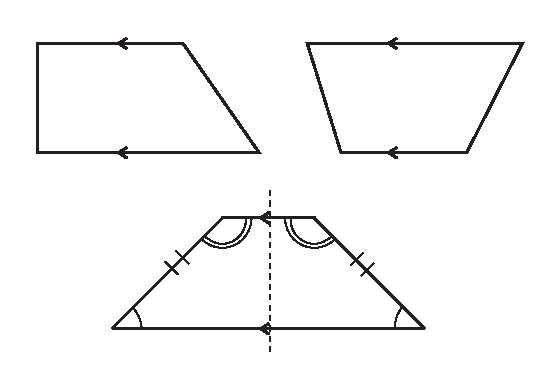
\includegraphics[width=3.5in]{ch6trapezium.eps}
\caption{Examples of trapeziums.}
\label{fig:m:gt:p:q:trapezium}
\end{center}
\end{figure}

\subsubsection{Parallelogram}
A trapezium with both sets of opposite sides parallel is called a \textit{parallelogram}. A summary of the properties of a parallelogram is:
\begin{itemize}
\item Both pairs of opposite sides are parallel.
\item Both pairs of opposite sides are equal in length.
\item Both pairs of opposite angles are equal.
\item Both diagonals bisect each other (i.e. they cut each other in half).
\end{itemize}

\begin{figure}[htb]
\begin{center}
\begin{pspicture}(0,-0.4)(5,2.8)
%\psgrid[gridcolor=gray]
\pstGeonode[PosAngle={180,0,0,180},CurveType=polygon](0.5,0){A}(4,0){B}(4.5,2.5){C}(1,2.5){D}
\pstSegmentMark{A}{B}
\pstSegmentMark{C}{D}
\pstSegmentMark[SegmentSymbol=MarkCros]{A}{D}
\pstSegmentMark[SegmentSymbol=MarkCros]{B}{C}
\pstLineAB[nodesep=0]{A}{C}
\pstLineAB[nodesep=0]{D}{B}
\pstMiddleAB[PointName=none]{A}{C}{O}
\pstSegmentMark[SegmentSymbol=pstslashhh]{A}{O}
\pstSegmentMark[SegmentSymbol=pstslashhh]{C}{O}
\pstSegmentMark[SegmentSymbol=pstslash]{D}{O}
\pstSegmentMark[SegmentSymbol=pstslash]{B}{O}
\pstSegmentMark[SegmentSymbol=>]{B}{O}
\pstMarkAngle[LabelSep=0.6]{B}{A}{D}{}
\pstMarkAngle[LabelSep=0.6]{D}{C}{B}{}
\pstMarkAngle[LabelSep=0.6, MarkAngleRadius = 0.3]{C}{B}{A}{}
\pstMarkAngle[LabelSep=0.6, MarkAngleRadius = 0.4]{C}{B}{A}{}
\pstMarkAngle[LabelSep=0.6, MarkAngleRadius = 0.3]{A}{D}{C}{}
\pstMarkAngle[LabelSep=0.4, MarkAngleRadius = 0.4]{A}{D}{C}{}
\end{pspicture}
\caption{An example of a parallelogram.}
\label{fig:mgt:p:q:parallelogram}
\end{center}
\end{figure}

\subsubsection{Rectangle}
A \textit{rectangle} is a parallelogram that has all four angles equal to $90^\circ$. A summary of the properties of a rectangle is:
\begin{itemize}
\item Both pairs of opposite sides are parallel.
\item Both pairs of opposite sides are of equal length.
\item Both diagonals bisect each other.
\item Diagonals are equal in length.
\item All angles at the corners are right angles.
\end{itemize}

\begin{figure}[htb]
\begin{center}
\begin{pspicture}(0,-0.4)(5,2.8)
%\psgrid[gridcolor=gray]
\pstGeonode[PosAngle={180,0,0,180},CurveType=polygon](0,0){A}(4,0){B}(4,2){C}(0,2){D}
\pstSegmentMark{A}{B}
\pstSegmentMark{C}{D}
\pstSegmentMark[SegmentSymbol=MarkCros]{A}{D}
\pstSegmentMark[SegmentSymbol=MarkCros]{B}{C}
\pstLineAB[nodesep=0]{A}{C}
\pstLineAB[nodesep=0]{D}{B}
\pstMiddleAB[PointName=none]{A}{C}{O}
\pstSegmentMark[SegmentSymbol=pstslash]{A}{O}
\pstSegmentMark[SegmentSymbol=pstslash]{C}{O}
\pstSegmentMark[SegmentSymbol=pstslash]{D}{O}
\pstSegmentMark[SegmentSymbol=pstslash]{B}{O}
\pstSegmentMark[SegmentSymbol=>]{B}{O}
\pstRightAngle[RightAngleSize=0.2,LabelSep=0.6]{B}{A}{D}
\pstRightAngle[RightAngleSize=0.2,LabelSep=0.6]{A}{D}{C}
\pstRightAngle[RightAngleSize=0.2,LabelSep=0.6]{D}{C}{B}
\pstRightAngle[RightAngleSize=0.2,LabelSep=0.6]{C}{B}{A}
\end{pspicture}
\caption{Example of a rectangle.}
\label{fig:mgt:p:q:rectangle}
\end{center}
\end{figure}

\subsubsection{Rhombus}
A \textit{rhombus} is a parallelogram that has all four sides of equal length. A summary of the properties of a rhombus is:
\begin{itemize}
\item Both pairs of opposite sides are parallel.
\item All sides are equal in length.
\item Both pairs of opposite angles are equal.
\item Both diagonals bisect each other at $90^\circ$.
\item Diagonals of a rhombus bisect both pairs of opposite angles.
\end{itemize}

\begin{figure}[htb]
\begin{center}
\begin{pspicture}(0,-0.4)(5,2.8)
%\psgrid[gridcolor=gray]
\pstGeonode[PosAngle={180,0,0,180},CurveType=polygon](0.5,0){A}(3,0){B}(3.5,2.5){C}(1,2.5){D}
\pstSegmentMark{A}{B}
\pstSegmentMark{C}{D}
\pstSegmentMark{A}{D}
\pstSegmentMark{B}{C}
\pstLineAB[nodesep=0]{A}{C}
\pstLineAB[nodesep=0]{D}{B}
\pstMiddleAB[PointName=none]{A}{C}{O}
\pstSegmentMark[SegmentSymbol=pstslashhh]{A}{O}
\pstSegmentMark[SegmentSymbol=pstslashhh]{C}{O}
\pstSegmentMark[SegmentSymbol=pstslash]{D}{O}
\pstSegmentMark[SegmentSymbol=pstslash]{B}{O}
\pstSegmentMark[SegmentSymbol=>]{B}{O}
\pstMarkAngle[LabelSep = 0.4, MarkAngleRadius = 0]{B}{A}{O}{x}
\pstMarkAngle[LabelSep = 0.4, MarkAngleRadius = 0]{O}{A}{D}{x}
\pstMarkAngle[LabelSep = 0.4, MarkAngleRadius = 0]{D}{C}{O}{x}
\pstMarkAngle[LabelSep = 0.4, MarkAngleRadius = 0]{O}{C}{B}{x}
\pstMarkAngle[LabelSep = 0.4, MarkAngleRadius = 0]{O}{D}{C}{$\bullet$}
\pstMarkAngle[LabelSep = 0.4, MarkAngleRadius = 0]{A}{D}{O}{$\bullet$}
\pstMarkAngle[LabelSep = 0.4, MarkAngleRadius = 0]{C}{B}{O}{$\bullet$}
\pstMarkAngle[LabelSep = 0.4, MarkAngleRadius = 0]{O}{B}{A}{$\bullet$}
\pstRightAngle{C}{O}{D}

\end{pspicture}
\caption{An example of a rhombus. A rhombus is a parallelogram with all sides equal.}
\label{fig:mgt:p:q:rhombus}
\end{center}
\end{figure}

\subsubsection{Square}
A \textit{square} is a rhombus that has all four angles equal to 90\deg. 

A summary of the properties of a rhombus is:
\begin{itemize}
\item Both pairs of opposite sides are parallel.
\item All sides are equal in length.
\item All angles are equal to $90^\circ$.
\item Both pairs of opposite angles are equal.
\item Both diagonals bisect each other at $90^\circ$.
\item Diagonals are equal in length.
\item Diagonals bisect both pairs of opposite angles (ie. all $45\degree$).
\end{itemize}

\begin{figure}[htb]
\begin{center}
\begin{pspicture}(0,-0.4)(5,4.5)
%\psgrid[gridcolor=gray]
\pstGeonode[PosAngle={180,0,0,180},CurveType=polygon](0,0){A}(4,0){B}(4,4){C}(0,4){D}
\pstSegmentMark{A}{B}
\pstSegmentMark{C}{D}
\pstSegmentMark{A}{D}
\pstSegmentMark{B}{C}
\pstLineAB[nodesep=0]{A}{C}
\pstLineAB[nodesep=0]{D}{B}
\pstMiddleAB[PointName=none]{A}{C}{O}
\pstSegmentMark[SegmentSymbol=pstslash]{A}{O}
\pstSegmentMark[SegmentSymbol=pstslash]{C}{O}
\pstSegmentMark[SegmentSymbol=pstslash]{D}{O}
\pstSegmentMark[SegmentSymbol=pstslash]{B}{O}
\pstSegmentMark[SegmentSymbol=>]{B}{O}
\pstRightAngle[RightAngleSize=0.2,LabelSep=0.6]{B}{A}{D}
\pstRightAngle[RightAngleSize=0.2,LabelSep=0.6]{A}{D}{C}
\pstRightAngle[RightAngleSize=0.2,LabelSep=0.6]{D}{C}{B}
\pstRightAngle[RightAngleSize=0.2,LabelSep=0.6]{C}{B}{A}
\pstRightAngle[RightAngleSize=0.2,LabelSep=0.6]{C}{O}{D}
\pstMarkAngle[LabelSep = 0.4, MarkAngleRadius = 0]{O}{D}{C}{$\bullet$}
\pstMarkAngle[LabelSep = 0.4, MarkAngleRadius = 0]{A}{D}{O}{$\bullet$}
\pstMarkAngle[LabelSep = 0.4, MarkAngleRadius = 0]{O}{A}{D}{$\bullet$}
\pstMarkAngle[LabelSep = 0.4, MarkAngleRadius = 0]{B}{A}{O}{$\bullet$}
\pstMarkAngle[LabelSep = 0.4, MarkAngleRadius = 0]{O}{B}{A}{$\bullet$}
\pstMarkAngle[LabelSep = 0.4, MarkAngleRadius = 0]{C}{B}{O}{$\bullet$}
\pstMarkAngle[LabelSep = 0.4, MarkAngleRadius = 0]{D}{C}{O}{$\bullet$}
\pstMarkAngle[LabelSep = 0.4, MarkAngleRadius = 0]{O}{C}{B}{$\bullet$}

\end{pspicture}
\caption{An example of a square. A square is a rhombus with all angles equal to 90\deg.}
\label{fig:mg:p:q:square}
\end{center}
\end{figure}

\subsubsection{Kite}
A \textit{kite} is a quadrilateral with two pairs of adjacent sides equal. 

A summary of the properties of a kite is:
\begin{itemize}
\item Two pairs of adjacent sides are equal in length.
\item One pair of opposite angles are equal where the angles are between unequal sides.
\item One diagonal bisects the other diagonal and one diagonal bisects one pair of opposite angles.
\item Diagonals intersect at right-angles.
\end{itemize}

\begin{figure}[htb]
\begin{center}
\begin{pspicture}(-0.6,-5)(4.6,3)
%\psgrid[gridcolor=gray]
\pstGeonode[PosAngle={180,0,90,270},CurveType=polygon](0,0){A}(4,0){B}(2,2.5){C}(2,-4.5){D}
\pstSegmentMark{A}{C}
\pstSegmentMark{B}{C}
\pstSegmentMark[SegmentSymbol=MarkCros]{A}{D}
\pstSegmentMark[SegmentSymbol=MarkCros]{B}{D}
\pstLineAB[nodesep=0]{A}{C}
\pstLineAB[nodesep=0]{D}{B}
\pstMiddleAB[PointName=none]{A}{B}{O}
\pstSegmentMark[SegmentSymbol=pstslash]{A}{O}
\pstSegmentMark[SegmentSymbol=pstslash]{B}{O}
\pstRightAngle{A}{O}{C}
\pstMarkAngle[LabelSep = 0.6, MarkAngleRadius = 0]{A}{C}{D}{x}
\pstMarkAngle[LabelSep = 0.6, MarkAngleRadius = 0]{D}{C}{B}{x}
\pstMarkAngle{C}{B}{D}{}
\pstMarkAngle{D}{A}{C}{}
\pstMarkAngle[LabelSep = 0.6, MarkAngleRadius = 0]{C}{D}{A}{$\bullet$}
\pstMarkAngle[LabelSep = 0.6, MarkAngleRadius = 0]{B}{D}{C}{$\bullet$}
\end{pspicture}
\caption{An example of a kite.}
\label{fig:mg:p:q:kite}
\end{center}
\end{figure}

\subsection{Other polygons}
\label{mg:p:o}
There are many other polygons, some of which are given in the table below.
\begin{table}[H]
\begin{center}
\begin{tabular}{|c|l|}
\hline
Sides & Name\\
\hline
5 & pentagon \\
6 & hexagon \\
7 & heptagon \\
8 & octagon \\
10 & decagon \\
15 & pentadecagon \\
\hline
\end{tabular}
\end{center}
\caption{Table of some polygons and their number of sides.}
\label{tb:mg:p:o}
\end{table}

\begin{figure}[htb]
\begin{center}
\begin{pspicture}(-1,-1)(5,3)
%\psgrid[gridcolor=gray]
\rput(0,0){\PstPolygon[PolyNbSides=5]}\rput(0,0){pentagon}
\rput(2,0){\PstPolygon[PolyNbSides=6]}\rput(2,0){hexagon}
\rput(4,0){\PstPolygon[PolyNbSides=7]}\rput(4,0){heptagon}
\rput(0,2){\PstPolygon[PolyNbSides=8]}\rput(0,2){octagon}
\rput(2,2){\PstPolygon[PolyNbSides=9]}\rput(2,2){nonagon}
\rput(4,2){\PstPolygon[PolyNbSides=10]}\rput(4,2){decagon}
\end{pspicture}
\caption{Examples of other polygons.}
\label{fig:mg:p:o:otherpolygons}
\end{center}
\end{figure}

\subsection{Extra}
\label{mg:p:e}

\subsubsection{Angles of Regular Polygons}
You can calculate the size of the interior angle of a regular polygon by using:
\begin{equation}
\label{eq:mg:p:e:angles}
\hat A = \frac{n-2}n \times 180^\circ
\end{equation}
where $n$ is the number of sides and $\hat A$ is any angle.

\subsubsection{Areas of Polygons}
\begin{enumerate}
\item{Area of triangle: $\frac 12\times$ base $\times$ perpendicular height}
\begin{pspicture}(0,-0.6)(1.72,0.43)
\pspolygon[linewidth=0.04](0.0,-0.39)(1.2,0.41)(1.7,-0.39)
\rput(.85,-.55){\footnotesize base}
\psline[linewidth=0.03cm,linestyle=dashed,dash=0.16cm 0.16cm](1.2,0.41)(1.2,-0.39)
\psframe[linewidth=0.02,dimen=outer](1.34,-0.25)(1.18,-0.41)
\usefont{T1}{ptm}{m}{n}
\rput(1.0979687,-0.055){\footnotesize h}
\end{pspicture} 
\item{Area of trapezium: $\frac{1}{2} \times$ (sum of $\parallel $ (parallel) sides) $\times$ perpendicular height}
\scalebox{1} % Change this value to rescale the drawing.
{
\begin{pspicture}(0,-0.42)(2.12,0.42)
\pspolygon[linewidth=0.04](0.8,0.4)(1.9,0.4)(2.1,-0.4)(0.0,-0.4)
\psline[linewidth=0.03cm,linestyle=dashed,dash=0.16cm 0.16cm](0.8,0.4)(0.8,-0.4)
\psframe[linewidth=0.02,dimen=outer](0.96,-0.24)(0.8,-0.4)
\usefont{T1}{ptm}{m}{n}
\rput(0.9579688,0.055){\footnotesize h}
\end{pspicture} 
}
\item{Area of parallelogram and rhombus: base $\times$ perpendicular height}
\scalebox{1} % Change this value to rescale the drawing.
{
\begin{pspicture}(0,-0.42)(2.02,0.42)
\pspolygon[linewidth=0.04](0.5,0.4)(2.0,0.4)(1.6,-0.4)(0.0,-0.4)
\psline[linewidth=0.03cm,linestyle=dashed,dash=0.16cm 0.16cm](0.8,0.4)(0.8,-0.4)
\psframe[linewidth=0.02,dimen=outer](0.96,-0.24)(0.8,-0.4)
\usefont{T1}{ptm}{m}{n}
\rput(0.99796873,0.015){\footnotesize h}
\end{pspicture} 
}
\item{Area of rectangle: length $\times$ breadth}
\scalebox{1} % Change this value to rescale the drawing.
{
\begin{pspicture}(0,-0.39)(1.8890625,0.39)
\psframe[linewidth=0.04,dimen=outer](1.62,0.39)(0.0,-0.39)
\psframe[linewidth=0.02,dimen=outer](0.16,-0.21)(0.0,-0.37)
\usefont{T1}{ptm}{m}{n}
\rput(1.775,0.065){\footnotesize b}
\usefont{T1}{ptm}{m}{n}
\rput(0.83640623,-0.195){\footnotesize l}
\end{pspicture} 
}

\item{Area of square: length of side $\times$ length of side}
\scalebox{1} % Change this value to rescale the drawing.
{
\begin{pspicture}(0,-0.6721875)(1.204375,0.6321875)
\psframe[linewidth=0.04,dimen=outer](1.204375,0.6321875)(0.224375,-0.3478125)
\usefont{T1}{ptm}{m}{n}
\rput(0.03328125,0.1871875){\footnotesize s}
\usefont{T1}{ptm}{m}{n}
\rput(0.67328125,-0.5328125){\footnotesize s}
\end{pspicture} 
}

\item Area of circle: $\pi$ x radius$^2$
\scalebox{1} % Change this value to rescale the drawing.
{
\begin{pspicture}(0,-0.72)(1.4,0.7)
\pscircle[linewidth=0.04,dimen=outer](0.7,0.0){0.7}
\psline[linewidth=0.04cm,dotsize=0.07055555cm 1.0]{*-}(0.7,0.0)(0.7,-0.7)
\usefont{T1}{ptm}{m}{n}
\rput(0.53328127,-0.225){\footnotesize r}
\end{pspicture} 
}
\end{enumerate}

\Exercise{Polygons}
{
\begin{enumerate}
\item For each case below, say whether the statement is true or false. For false statements, give a counter-example to prove it:
\begin{enumerate}
\item All squares are rectangles
\item All rectangles are squares
\item All pentagons are similar
\item All equilateral triangles are similar
\item All pentagons are congruent
\item All equilateral triangles are congruent
\end{enumerate}
\item Find the areas of each of the given figures - remember area is measured in square units (cm$^2$, m$^2$, mm$^2$). \\

\scalebox{0.9}
{
\begin{pspicture}(0,-4.758281)(14.921875,4.758281) \psline[linewidth=0.04cm](0.381875,1.7882812)(4.381875,1.7882812) \psline[linewidth=0.04cm](4.241875,1.7682812)(4.241875,1.7682812) \psline[linewidth=0.04cm,linestyle=dashed,dash=0.16cm 0.16cm](2.361875,3.8082812)(2.361875,2.8282812) \psline[linewidth=0.04cm](0.381875,1.7882812)(2.341875,3.7882812) \psline[linewidth=0.04cm](2.361875,3.7882812)(4.341875,1.8282813) \usefont{T1}{ptm}{m}{n} \rput(2.4517188,2.5782812){5cm} \psline[linewidth=0.04cm,linestyle=dashed,dash=0.16cm 0.16cm](2.361875,2.3482811)(2.361875,1.7682812) \usefont{T1}{ptm}{m}{n} \rput(2.4365625,1.4182812){10cm} \usefont{T1}{ptm}{m}{n} \rput(0.16203125,3.6182814){a)} \psframe[linewidth=0.04,dimen=outer](9.141875,3.7782812)(5.141875,1.7782812) \usefont{T1}{ptm}{m}{n} \rput(4.72375,3.5982811){b)} \psframe[linewidth=0.04,dimen=outer](5.471875,3.7782812)(5.151875,3.4582813) \psline[linewidth=0.04cm](7.121875,3.9282813)(7.321875,3.7682812) \psline[linewidth=0.04cm](7.1272163,3.6020272)(7.3165336,3.7745354) \psline[linewidth=0.04cm](7.121875,1.9482813)(7.321875,1.7882812) \psline[linewidth=0.04cm](7.1272163,1.6220272)(7.3165336,1.7945354) \psline[linewidth=0.04cm](4.995617,2.7704508)(5.161965,2.965203) \psline[linewidth=0.04cm](5.321874,2.7652996)(5.1555424,2.9600654) \psline[linewidth=0.04cm](4.995617,2.570451)(5.161965,2.765203) \psline[linewidth=0.04cm](5.321874,2.5652997)(5.1555424,2.7600653) \psline[linewidth=0.04cm](8.955617,2.7704508)(9.121964,2.965203) \psline[linewidth=0.04cm](9.281874,2.7652996)(9.115542,2.9600654) \psline[linewidth=0.04cm](8.955617,2.590451)(9.121964,2.785203) \psline[linewidth=0.04cm](9.281874,2.5852997)(9.115542,2.7800653) \usefont{T1}{ptm}{m}{n} \rput(9.711719,2.7182813){5cm} \usefont{T1}{ptm}{m}{n} \rput(7.1965623,1.4182812){10cm} \psline[linewidth=0.04cm,linestyle=dashed,dash=0.16cm 0.16cm](10.901875,2.7482812)(14.901875,2.7482812) \pscircle[linewidth=0.04,dimen=outer](12.911875,2.7582812){2.0} \psdots[dotsize=0.16](12.901875,2.7482812) \usefont{T1}{ptm}{m}{n} \rput(12.876562,2.4182813){10cm} \usefont{T1}{ptm}{m}{n} \rput(10.631406,3.5982811){c)} \usefont{T1}{ptm}{m}{n} \rput(0.19140625,0.19828124){d)} \usefont{T1}{ptm}{m}{n} \rput(5.5117188,-0.8017188){5cm} \usefont{T1}{ptm}{m}{n} \rput(2.5340624,0.29828125){7cm} \psline[linewidth=0.04cm](2.1600447,-1.3315424)(2.358717,-1.4931878) \psline[linewidth=0.04cm](2.162693,-1.6578295)(2.3534274,-1.4868897) \psline[linewidth=0.04cm](1.9601017,-1.3363228)(2.1587741,-1.4979682) \psline[linewidth=0.04cm](1.9627501,-1.6626099)(2.1534846,-1.4916701) \psline[linewidth=0.04cm](0.181875,-1.4917188)(4.181875,-1.4917188) \psline[linewidth=0.04cm](1.401875,0.04828125)(5.401875,0.04828125) \psline[linewidth=0.04cm](3.3800445,0.2084576)(3.578717,0.046812218) \psline[linewidth=0.04cm](3.382693,-0.11782951)(3.5734274,0.053110242) \psline[linewidth=0.04cm](3.1801016,0.20367722)(3.3787742,0.042031832) \psline[linewidth=0.04cm](3.18275,-0.1226099)(3.3734844,0.048329853) \psline[linewidth=0.04cm](4.191091,-1.5022907)(5.394185,0.045147188) \psline[linewidth=0.04cm](4.621163,-0.6958544)(4.8714867,-0.6416498) \psline[linewidth=0.04cm](4.877642,-0.89756864)(4.863264,-0.64184755) \psline[linewidth=0.04cm](0.21109095,-1.4822907)(1.4141852,0.065147184) \psline[linewidth=0.04cm](0.641163,-0.67585444)(0.89148647,-0.6216498) \psline[linewidth=0.04cm](0.8976424,-0.87756866)(0.8832641,-0.62184757) \psline[linewidth=0.04cm,linestyle=dashed,dash=0.16cm 0.16cm](4.161875,-1.4917188)(4.161875,0.04828125) \psframe[linewidth=0.04,dimen=outer](4.471875,0.05828125)(4.151875,-0.26171875) \usefont{T1}{ptm}{m}{n} \rput(4.7753124,0.27828124){3cm} \psline[linewidth=0.04cm](6.021875,-1.4317187)(10.021875,-1.4317187) \psline[linewidth=0.04cm](9.821875,-1.4517188)(9.821875,-1.4517188) \usefont{T1}{ptm}{m}{n} \rput(7.5165625,-1.7217188){12cm} \psline[linewidth=0.04cm](8.837452,0.20483598)(10.026298,-1.4282734) \psline[linewidth=0.04cm](8.821875,0.20828125)(6.021875,-1.4317187) \psline[linewidth=0.04cm,linestyle=dashed,dash=0.16cm 0.16cm](8.821875,0.18828125)(8.821875,-1.4117187) \psframe[linewidth=0.04,dimen=outer](8.851875,-1.1217188)(8.531875,-1.4417187) \usefont{T1}{ptm}{m}{n} \rput(9.217969,-1.6817187){8cm} \usefont{T1}{ptm}{m}{n} \rput(9.936563,-0.44171876){10cm} \usefont{T1}{ptm}{m}{n} \rput(6.2414064,0.23828125){e)} \psline[linewidth=0.04cm](11.561875,-1.3517188)(13.581875,-1.3517188) \psline[linewidth=0.04cm](11.564406,-1.3656596)(12.099343,0.58222204) \psline[linewidth=0.04cm](12.107254,0.5571398)(13.576495,-1.3405774) \psline[linewidth=0.04cm](11.621875,-0.49171874)(11.941875,-0.59171873) \psline[linewidth=0.04cm](11.681875,-0.35171875)(12.001875,-0.45171875) \psline[linewidth=0.04cm](12.161875,-1.1917187)(12.161875,-1.5317187) \psline[linewidth=0.04cm](12.161875,-1.4317187)(12.161875,-1.4317187) \psline[linewidth=0.04cm](12.321875,-1.1917187)(12.321875,-1.5317187) \usefont{T1}{ptm}{m}{n} \rput(11.094063,0.23828125){f)} \usefont{T1}{ptm}{m}{n} \rput(12.7517185,-1.6417187){5cm} \usefont{T1}{ptm}{m}{n} \rput(13.181562,-0.18171875){6cm} \pstriangle[linewidth=0.04,dimen=outer](2.031875,-4.491719)(3.4,2.4) %\pstriangle[linewidth=0.04,dimen=outer](3.181875,-2.6717188)(0.0,0.0) %\pstriangle[linewidth=0.04,dimen=outer](3.161875,-2.7517188)(0.0,0.0) %\pstriangle[linewidth=0.04,dimen=outer](3.001875,-2.5317187)(0.0,0.0) 
\usefont{T1}{ptm}{m}{n} \rput(0.23140626,-2.2617188){g)} \psline[linewidth=0.04cm](1.901875,-4.331719)(1.901875,-4.6517186) \psline[linewidth=0.04cm](1.101875,-3.1117187)(1.341875,-3.3317187) \psline[linewidth=0.04cm](2.6844237,-3.3744361)(2.9193263,-3.1490014) \usefont{T1}{ptm}{m}{n} \rput(3.6565626,-3.1417189){10cm} \pspolygon[linewidth=0.04](5.201875,-4.371719)(9.201875,-4.371719)(8.181875,-2.6717188)(6.181875,-2.6717188)(6.001875,-2.9717188) \psline[linewidth=0.04cm](6.161875,-2.6717188)(6.161875,-2.6717188) \psline[linewidth=0.04cm](6.161875,-2.6717188)(6.161875,-2.6717188) \psline[linewidth=0.04cm,linestyle=dashed,dash=0.16cm 0.16cm](6.161875,-2.6717188)(6.161875,-4.351719) \psline[linewidth=0.04cm](7.106746,-2.5312762)(7.309965,-2.6871674) \psline[linewidth=0.04cm](7.118735,-2.8573537)(7.3044972,-2.6810234) \psline[linewidth=0.04cm](7.106746,-4.211276)(7.309965,-4.3671675) \psline[linewidth=0.04cm](7.118735,-4.5373535)(7.3044972,-4.3610234) \psframe[linewidth=0.04,dimen=outer](6.471875,-4.061719)(6.151875,-4.3817186) \usefont{T1}{ptm}{m}{n} \rput(5.3565626,-2.9817188){15cm} \usefont{T1}{ptm}{m}{n} \rput(5.5398436,-4.601719){9cm} \usefont{T1}{ptm}{m}{n} \rput(7.6565623,-2.4017189){16cm} \usefont{T1}{ptm}{m}{n} \rput(7.9285936,-4.601719){21cm} \usefont{T1}{ptm}{m}{n} \rput(5.08375,-2.2617188){h)} \end{pspicture}
}
\end{enumerate}
}

\section{Exercises}
\begin{enumerate}
\item Find all the pairs of parallel lines in the following figures, giving reasons in each case.
\begin{multicols}{2}
\item[(a)] \scalebox{0.8}{\begin{pspicture}(0,-1.6034375)(5.1659374,1.6034375) \psline[linewidth=0.04cm](0.476875,1.203125)(4.716875,1.203125) \psline[linewidth=0.04cm](0.476875,-1.096875)(4.716875,-1.096875) \psline[linewidth=0.04cm](0.476875,1.203125)(4.676875,-1.096875)
\rput(3.1875,-0.766875){62$^{\circ}$}
\rput(2.2275,0.853125){62$^{\circ}$}
\rput(0.1175,1.413125){A} 
\rput(4.97625,1.313125){B}
\rput(0.22578125,-1.406875){D} 
\rput(5.0021877,-1.446875){C} 
\end{pspicture} }
\item[(c)]
\scalebox{0.7}{\begin{pspicture}(0,-2.66)(7.791875,2.66) \psline[linewidth=0.04cm](0.7065625,1.72)(6.1865625,1.72) \psline[linewidth=0.04cm](0.0065625,-1.48)(5.5265627,-1.48) \psline[linewidth=0.04cm](1.5465626,2.64)(0.4665625,-2.44) \psline[linewidth=0.04cm](5.8465624,2.44)(4.7665625,-2.64)  \rput(6.5721874,1.27){120$^{\circ}$} 
\rput(1.7135937,-1.15){60$^{\circ}$} 
\rput(4.1135936,-1.91){60$^{\circ}$} 
\rput(1.051875,2.17){G}
\rput(6.1254687,2.05){H} 
\rput(0.06421875,-1.89){K} 
\rput(5.443594,-1.97){L} 
\end{pspicture} }
\item[(b)]
\scalebox{0.65}{
\begin{pspicture}(0,-2.7134376)(8.0,2.7134376) \psline[linewidth=0.04cm](0.64,2.153125)(1.94,-2.526875) \psline[linewidth=0.04cm](5.8,2.553125)(7.1,-2.126875) \psline[linewidth=0.04cm](0.0,1.513125)(7.24,2.153125) \psline[linewidth=0.04cm](0.74,-2.126875)(7.98,-1.486875)  \rput(0.1615625,2.023125){M} 
\rput(6.3395314,2.523125){N} 
\rput(1.4215626,-2.556875){O} 
\rput(7.5796876,-1.956875){P} 
\rput(6.7807813,1.743125){57$^{\circ}$}
\rput(6.485625,-1.956875){123$^{\circ}$} 
\rput(1.505625,1.983125){137$^{\circ}$} 
\end{pspicture}}
\end{multicols}

%\newpage
\item Find angles $a$, $b$, $c$ and $d$ in each case, giving reasons. 
\begin{enumerate} 
\item[(a)] 
{\begin{pspicture}(0,-1.5101563)(4.01,1.5101563) \psline[linewidth=0.04cm](0.0,-0.15015624)(2.98,-1.1301563) \psline[linewidth=0.04cm](3.0,0.22984375)(0.96,1.1298437) \psline[linewidth=0.04cm](2.98,0.22984375)(2.98,-1.1501563) \psline[linewidth=0.04cm](0.98,1.1098437)(1.0,-0.47015625) \psline[linewidth=0.02cm](1.7,-0.5701563)(1.9,-0.7501562) \psline[linewidth=0.02cm](1.6,-0.85015625)(1.9,-0.79015625) \psline[linewidth=0.02cm](1.86,0.90984374)(2.08,0.64984375) \psline[linewidth=0.02cm](1.72,0.6298438)(2.02,0.6298438) \psline[linewidth=0.02cm](0.84,0.22984375)(0.98,-0.05015625) \psline[linewidth=0.02cm](0.98,-0.05015625)(0.98,-0.05015625) \psline[linewidth=0.02cm](0.98,-0.01015625)(1.12,0.20984375) \psline[linewidth=0.02cm](0.76,0.12984376)(0.98,-0.21015625) \psline[linewidth=0.02cm](0.98,-0.21015625)(1.18,0.12984376) \psline[linewidth=0.02cm](2.78,-0.37015626)(2.96,-0.71015626) \psline[linewidth=0.02cm](2.96,-0.71015626)(3.08,-0.37015626) \psline[linewidth=0.02cm](2.72,-0.43015626)(2.96,-0.83015627) \psline[linewidth=0.02cm](2.96,-0.83015627)(3.14,-0.43015626) \psline[linewidth=0.02cm](4.0,-1.0701562)(4.0,-1.0701562) \rput(0.9196875,1.3198438){P} \rput(3.1346874,0.35984376){Q} \rput(3.0753126,-1.3601563){R} \rput(0.89921874,-0.74015623){S} \rput(2.8010938,0.11484375){\small a} \rput(1.1614063,0.77484375){\small b} \rput(1.1696875,-0.34515625){\small c} \rput(0.76140624,-0.24515624){\small d} \rput(2.6165626,-0.79015625){\footnotesize $73^{\circ}$} \end{pspicture} } 
\begin{multicols}{2}
\item[(b)] { \begin{pspicture}(0,-2.0301561)(3.6778126,2.0301561) \psline[linewidth=0.04cm](0.2865625,1.1098437)(3.3065624,1.1098437) \psline[linewidth=0.04cm](0.2865625,0.08984375)(3.2665625,0.08984375) \psline[linewidth=0.04cm](0.2865625,-0.89015627)(3.2865624,-0.89015627) \usefont{T1}{ptm}{m}{n} \rput(0.1271875,1.0998437){A} \usefont{T1}{ptm}{m}{n} \rput(3.5059376,1.1398437){B} \usefont{T1}{ptm}{m}{n} \rput(0.091875,0.03984375){C} \usefont{T1}{ptm}{m}{n} \rput(3.4954689,0.11984375){D} \usefont{T1}{ptm}{m}{n} \rput(0.043125,-0.9401562){E} \usefont{T1}{ptm}{m}{n} \rput(3.479375,-0.90015626){F} \psline[linewidth=0.04cm](2.1665626,1.6898438)(1.2265625,-1.5901562) \usefont{T1}{ptm}{m}{n} \rput(2.3242188,1.8398438){K} \usefont{T1}{ptm}{m}{n} \rput(2.1435938,0.83984375){L} \usefont{T1}{ptm}{m}{n} \rput(1.868125,-0.16015625){M} \usefont{T1}{ptm}{m}{n} \rput(1.2660937,-1.8801563){O} \usefont{T1}{ptm}{m}{n} \rput(1.608125,-1.1401563){N} \usefont{T1}{ptm}{m}{n} \rput(1.7076563,0.97484374){\small a} \usefont{T1}{ptm}{m}{n} \rput(1.9679687,0.27484375){\small b} \usefont{T1}{ptm}{m}{n} \rput(1.67625,-0.6851562){\small c} \usefont{T1}{ptm}{m}{n} \rput(1.1479688,-1.1051563){\small d} \usefont{T1}{ptm}{m}{n} \rput(1.5776563,1.3348438){\small $100^{\circ}$} \psline[linewidth=0.04cm](0.5665625,1.2898438)(0.9265625,1.1098437) \psline[linewidth=0.04cm](0.6065625,0.88984376)(0.8665625,1.1098437) \psline[linewidth=0.04cm](0.5665625,0.26984376)(0.8865625,0.10984375) \psline[linewidth=0.04cm](0.5865625,-0.11015625)(0.5865625,-0.11015625) \psline[linewidth=0.04cm](0.5865625,-0.11015625)(0.8465625,0.06984375) \psline[linewidth=0.04cm](0.5465625,-0.71015626)(0.8465625,-0.8701562) \psline[linewidth=0.04cm](0.5865625,-1.0901562)(0.8065625,-0.89015627) \end{pspicture} } 

\item[(c)] { \begin{pspicture}(0,-1.8901563)(3.724375,1.8901563) \psline[linewidth=0.064cm](0.256875,0.50984377)(0.256875,-1.4901563) \psline[linewidth=0.064cm](3.256875,1.5098437)(3.296875,-0.45015624) \psline[linewidth=0.064cm](0.236875,-1.4501562)(3.296875,1.5498438) \psline[linewidth=0.064cm](0.256875,0.52984375)(3.276875,-0.45015624) \psline[linewidth=0.02cm](0.076875,-0.67015624)(0.236875,-0.21015625) \psline[linewidth=0.02cm](0.276875,-0.25015625)(0.416875,-0.67015624) \psline[linewidth=0.02cm](3.076875,0.20984375)(3.276875,0.64984375) \psline[linewidth=0.02cm](3.256875,0.6298438)(3.476875,0.24984375) \rput(0.10765625,0.63984376){T} \rput(1.7901562,-0.28015625){U} \rput(3.490625,-0.74015623){V} \rput(3.5304687,1.6998438){W} \rput(0.1634375,-1.7401563){X} \rput(3.0579689,-0.16515625){\small a} \rput(0.43828124,-0.9451563){\small b} \rput(1.3065625,-0.06515625){\small d} \rput(1.6782813,0.29484376){\small c} \rput(2.9854689,0.9348438){\small $45^{\circ}$} \rput(0.5106875,0.18984374){\footnotesize $50^{\circ}$} \end{pspicture} } 
\end{multicols}
\end{enumerate}


\begin{enumerate} \item Which of the following claims are true? Give a counter-example for those that are incorrect. \begin{enumerate} \item All equilateral triangles are similar. \\ \item All regular quadrilaterals are similar. \\ \item In any $\triangle ABC$ with $\angle ABC = 90^{\circ}$ we have $AB^3+BC^3=CA^3$. \\ \item All right-angled isosceles triangles with perimeter 10~cm are congruent. \\ \item All rectangles with the same area are similar. \end{enumerate} \item Say which of the following pairs of triangles are congruent with reasons. \begin{enumerate} \item { \begin{pspicture}(0,-1.7101562)(6.965625,1.7101562) \psline[linewidth=0.02cm](1.2465625,1.1498437)(0.2865625,-1.4101562) \psline[linewidth=0.02cm](0.3265625,-1.3901563)(2.5665624,-0.97015625) \psline[linewidth=0.02cm](1.2465625,1.1298437)(2.5065625,-0.9501563) \psline[linewidth=0.02cm](5.4865627,1.3098438)(4.4065623,-1.1101563) \psline[linewidth=0.02cm](4.4065623,-1.1101563)(6.6065626,-0.53015625) \psline[linewidth=0.02cm](5.4865627,1.2898438)(6.5665627,-0.5101563) \psline[linewidth=0.02cm](1.4265625,-1.0701562)(1.4865625,-1.2701563) \psline[linewidth=0.02cm](5.5665627,-0.65015626)(5.6465626,-0.97015625) \psline[linewidth=0.02cm](0.6065625,-0.07015625)(0.8465625,-0.15015624) \psline[linewidth=0.02cm](0.5465625,-0.17015626)(0.8065625,-0.27015626) \psline[linewidth=0.02cm](4.8265624,0.16984375)(5.0465627,0.06984375) \psline[linewidth=0.02cm](4.8865623,0.30984375)(5.1065626,0.18984374) \psline[linewidth=0.02cm](1.6465625,0.14984375)(1.9465625,0.30984375) \psline[linewidth=0.02cm](1.7065625,0.06984375)(2.0065625,0.20984375) \psline[linewidth=0.02cm](1.7665625,-0.03015625)(2.0665624,0.10984375) \psline[linewidth=0.02cm](5.8665624,0.46984375)(6.1065626,0.56984377) \psline[linewidth=0.02cm](5.9265623,0.36984375)(6.1465626,0.46984375) \psline[linewidth=0.02cm](5.9865627,0.24984375)(6.2065625,0.34984374) \rput(1.2671875,1.3598437){A} \rput(0.0459375,-1.5601562){B} \rput(2.751875,-1.1201563){C} \rput(5.4754686,1.5198437){D} \rput(4.203125,-1.2201562){E} \rput(6.819375,-0.60015625){F} \end{pspicture} } \item { \begin{pspicture}(0,-1.6132812)(6.9140625,1.6132812) \psline[linewidth=0.02cm](0.2665625,1.1867187)(0.2465625,-1.2932812) \psline[linewidth=0.02cm](0.2465625,-1.2932812)(2.4665625,-1.2532812) \psline[linewidth=0.02cm](2.4665625,-1.2732812)(0.2665625,1.1867187) \psline[linewidth=0.02cm](3.2665625,0.7867187)(4.6065626,-0.8932812) \psline[linewidth=0.02cm](4.5865626,-0.8932812)(6.5865626,0.88671875) \psline[linewidth=0.02cm](3.2865624,0.7867187)(6.5665627,0.88671875) \psline[linewidth=0.02cm](0.2465625,-0.9532812)(0.6265625,-0.9532812) \psline[linewidth=0.02cm](0.6265625,-0.9532812)(0.6265625,-1.2532812) \psline[linewidth=0.02cm](4.4265623,-0.69328123)(4.6865625,-0.49328125) \psline[linewidth=0.02cm](4.6865625,-0.5132812)(4.8065624,-0.67328125) \psline[linewidth=0.02cm](1.3065625,-0.19328125)(1.5265625,0.02671875) \psline[linewidth=0.02cm](4.7065625,1.0467187)(4.7065625,0.68671876) \psline[linewidth=0.02cm](0.0665625,-0.01328125)(0.4665625,-0.01328125) \psline[linewidth=0.02cm](0.0665625,-0.17328125)(0.4865625,-0.17328125) \psline[linewidth=0.02cm](4.0865626,0.16671875)(3.7065625,-0.05328125) \psline[linewidth=0.02cm](4.1665626,0.06671875)(3.8065624,-0.15328126) \rput(0.131875,1.4167187){G} \rput(0.06546875,-1.4632813){H} \rput(2.585,-1.3232813){I} \rput(3.1226563,0.71671873){J} \rput(4.584219,-1.1832813){K} \rput(6.7635937,0.8567188){L} \end{pspicture} } \item { \begin{pspicture}(0,-1.6734375)(8.350625,1.6734375) \psline[linewidth=0.02cm](1.8665625,1.033125)(0.3465625,-1.346875) \psline[linewidth=0.02cm](0.3465625,-1.346875)(3.1265626,-1.286875) \psline[linewidth=0.02cm](3.1265626,-1.286875)(1.8665625,1.053125) \psline[linewidth=0.02cm](6.4265623,1.273125)(4.8065624,-1.166875) \psline[linewidth=0.02cm](4.8065624,-1.166875)(8.026563,-1.146875) \psline[linewidth=0.02cm](8.026563,-1.146875)(6.4265623,1.253125) \psarc[linewidth=0.02](8.246563,1.073125){0.0}{0.0}{180.0} \pscustom[linewidth=0.02] { \newpath \moveto(7.7465625,-0.746875) \lineto(7.6965623,-0.816875) \curveto(7.6715627,-0.851875)(7.6365623,-0.906875)(7.6265626,-0.926875) \curveto(7.6165624,-0.946875)(7.5915623,-0.991875)(7.5765624,-1.016875) \curveto(7.5615625,-1.041875)(7.5415626,-1.081875)(7.5265627,-1.126875) } \pscustom[linewidth=0.02] { \newpath \moveto(0.6265625,-0.886875) \lineto(0.6965625,-0.946875) \curveto(0.7315625,-0.976875)(0.7765625,-1.021875)(0.7865625,-1.036875) \curveto(0.7965625,-1.051875)(0.8165625,-1.086875)(0.8265625,-1.106875) \curveto(0.8365625,-1.126875)(0.8515625,-1.171875)(0.8565625,-1.196875) \curveto(0.8615625,-1.221875)(0.8565625,-1.261875)(0.8465625,-1.276875) \curveto(0.8365625,-1.291875)(0.8265625,-1.311875)(0.8265625,-1.326875) } \pscustom[linewidth=0.02] { \newpath \moveto(1.6665626,0.773125) \lineto(1.7365625,0.713125) \curveto(1.7715625,0.683125)(1.8315625,0.648125)(1.8565625,0.643125) \curveto(1.8815625,0.638125)(1.9365625,0.633125)(1.9665625,0.633125) \curveto(1.9965625,0.633125)(2.0365624,0.648125)(2.0665624,0.693125) } \pscustom[linewidth=0.02] { \newpath \moveto(1.6065625,0.593125) \lineto(1.6865625,0.543125) \curveto(1.7265625,0.518125)(1.7915626,0.488125)(1.8165625,0.483125) \curveto(1.8415625,0.478125)(1.8865625,0.468125)(1.9065624,0.463125) \curveto(1.9265625,0.458125)(1.9715625,0.453125)(1.9965625,0.453125) \curveto(2.0215626,0.453125)(2.0665624,0.463125)(2.0865624,0.473125) \curveto(2.1065626,0.483125)(2.1315625,0.493125)(2.1465626,0.493125) } \pscustom[linewidth=0.02] { \newpath \moveto(6.2465625,1.013125) \lineto(6.3265624,0.963125) \curveto(6.3665624,0.938125)(6.4315624,0.913125)(6.4565625,0.913125) \curveto(6.4815626,0.913125)(6.5315623,0.918125)(6.5565624,0.923125) \curveto(6.5815625,0.928125)(6.6115627,0.933125)(6.6265626,0.933125) } \pscustom[linewidth=0.02] { \newpath \moveto(6.1665626,0.833125) \lineto(6.2565627,0.813125) \curveto(6.3015623,0.803125)(6.3715625,0.793125)(6.3965626,0.793125) \curveto(6.4215627,0.793125)(6.4715624,0.793125)(6.4965625,0.793125) \curveto(6.5215626,0.793125)(6.5665627,0.798125)(6.5865626,0.803125) \curveto(6.6065626,0.808125)(6.6415625,0.818125)(6.6865625,0.833125) } \psline[linewidth=0.02cm](1.6865625,-1.086875)(1.6865625,-1.526875) \psline[linewidth=0.02cm](6.2065625,-0.906875)(6.1865625,-1.326875) \rput(0.088125,-1.476875){M} \rput(1.8460938,1.203125){N} \rput(3.288125,-1.516875){O} \rput(6.38625,1.483125){P} \rput(4.56125,-1.276875){Q} \rput(8.181875,-1.176875){R} \end{pspicture} } \item { \begin{pspicture}(0,-1.91625)(9.015312,1.91625) \psline[linewidth=0.02cm](2.1815624,0.8959375)(0.3215625,-1.6240625) \psline[linewidth=0.02cm](0.3215625,-1.6240625)(3.5215626,-1.2040625) \psline[linewidth=0.02cm](2.1815624,0.8759375)(3.4815626,-1.1840625) \psline[linewidth=0.02cm](7.1215625,1.5359375)(5.4615626,-1.2040625) \psline[linewidth=0.02cm](5.4615626,-1.2040625)(8.621563,-0.2040625) \psline[linewidth=0.02cm](8.621563,-0.2040625)(7.1215625,1.5359375) \psline[linewidth=0.02cm](1.3015625,-0.0040625)(1.6615624,-0.2040625) \psline[linewidth=0.02cm](6.2815623,0.5559375)(6.7615623,0.2559375) \psline[linewidth=0.02cm](1.7215625,-1.2040625)(1.7215625,-1.7040625) \psline[linewidth=0.02cm](1.9215626,-1.1840625)(1.9215626,-1.6240625) \psline[linewidth=0.02cm](6.6215625,-0.6240625)(6.7815623,-0.9640625) \psline[linewidth=0.02cm](6.8215623,-0.5640625)(7.0015626,-0.9040625) \pscustom[linewidth=0.02] { \newpath \moveto(0.6215625,-1.2040625) \lineto(0.6815625,-1.2540625) \curveto(0.7115625,-1.2790625)(0.7565625,-1.3240625)(0.7715625,-1.3440624) \curveto(0.7865625,-1.3640625)(0.8115625,-1.3990625)(0.8215625,-1.4140625) \curveto(0.8315625,-1.4290625)(0.8515625,-1.4640625)(0.8615625,-1.4840626) \curveto(0.8715625,-1.5040625)(0.8765625,-1.5290625)(0.8615625,-1.5440625) } \pscustom[linewidth=0.02] { \newpath \moveto(5.7415624,-0.7640625) \lineto(5.8115625,-0.7740625) \curveto(5.8465624,-0.7790625)(5.9115624,-0.8240625)(5.9415627,-0.8640625) \curveto(5.9715624,-0.9040625)(6.0115623,-0.9640625)(6.0215626,-0.9840625) \curveto(6.0315623,-1.0040625)(6.0415626,-1.0290625)(6.0415626,-1.0440625) } \rput(0.11625,-1.7140625){Q} \rput(2.156875,1.0459375){R} \rput(3.6407812,-1.2740625){S} \rput(5.2523437,-1.3140625){T} \rput(7.034844,1.7259375){U} \rput(8.855312,-0.2740625){V} \end{pspicture} } \end{enumerate} 
\item For each pair of figures state whether they are similar or not. Give reasons. \\ \scalebox{1}  { \begin{pspicture}(0,-3.8498437)(8.2225,3.8498437) \psline[linewidth=0.04cm](0.8984375,3.2101562)(0.8984375,1.1901562) \psline[linewidth=0.04cm](0.8984375,1.1901562)(2.8984375,1.1901562) \psline[linewidth=0.04cm](0.8984375,3.2101562)(2.8784375,1.2101562) \psframe[linewidth=0.04,dimen=outer](1.1184375,1.3901563)(0.8984375,1.1701562) \usefont{T1}{ptm}{m}{n} \rput(2.3360937,2.3401563){2$\sqrt{2}$} \usefont{T1}{ptm}{m}{n} \rput(0.63640624,2.1601562){2} \psline[linewidth=0.04cm](4.8984375,3.1901562)(4.8984375,0.21015625) \psline[linewidth=0.04cm](4.8984375,0.21015625)(7.9184375,0.23015624) \psline[linewidth=0.04cm](4.8984375,3.1701562)(7.9584374,0.21015625) \psframe[linewidth=0.04,dimen=outer](5.1184373,0.41015625)(4.8984375,0.19015625) \pscustom[linewidth=0.04] { \newpath \moveto(2.5784376,1.4901563) \lineto(2.5384376,1.4501562) \curveto(2.5184374,1.4301562)(2.4884374,1.3851563)(2.4784374,1.3601563) \curveto(2.4684374,1.3351562)(2.4534376,1.2901562)(2.4484375,1.2701563) \curveto(2.4434376,1.2501563)(2.4434376,1.2251563)(2.4584374,1.2101562) } \usefont{T1}{ptm}{m}{n} \rput(4.6542187,1.6201563){3} \usefont{T1}{ptm}{m}{n} \rput(6.394219,-0.07984375){3} \usefont{T1}{ptm}{m}{n} \rput(2.151875,1.4201562){45$^{\circ}$} \usefont{T1}{ptm}{m}{n} \rput(5.211875,2.4601562){45$^{\circ}$} \pscustom[linewidth=0.04] { \newpath \moveto(4.8984375,2.7301562) \lineto(4.9584374,2.7501562) \curveto(4.9884377,2.7601562)(5.0334377,2.7801561)(5.0484376,2.7901564) \curveto(5.0634375,2.8001564)(5.0884376,2.8251562)(5.0984373,2.8401563) \curveto(5.1084375,2.8551562)(5.1284375,2.8851562)(5.1384373,2.9001563) } \usefont{T1}{ptm}{m}{n} \rput(0.9190625,3.4001563){A} \usefont{T1}{ptm}{m}{n} \rput(0.8978125,0.92015624){B} \usefont{T1}{ptm}{m}{n} \rput(3.02375,0.9401562){C} \usefont{T1}{ptm}{m}{n} \rput(4.858125,3.3601563){P} \usefont{T1}{ptm}{m}{n} \rput(4.893125,-0.03984375){Q} \usefont{T1}{ptm}{m}{n} \rput(8.05375,-0.03984375){R} \usefont{T1}{ptm}{m}{n} \rput(0.206875,3.5){(a)} \usefont{T1}{ptm}{m}{n} \rput(0.206875,-1.0){(b)} 
\psframe[linewidth=0.04,dimen=outer](3.8984375,-1.3898437)(0.8984375,-3.3898437) \psframe[linewidth=0.04,dimen=outer](1.1584375,-1.4098438)(0.8984375,-1.6698438) \psframe[linewidth=0.04,dimen=outer](3.8784375,-1.3698437)(3.6184375,-1.6298437) \psframe[linewidth=0.04,dimen=outer](1.1584375,-3.1298437)(0.8984375,-3.3898437) \psframe[linewidth=0.04,dimen=outer](3.8984375,-3.1298437)(3.6384375,-3.3898437) \psframe[linewidth=0.04,dimen=outer](7.9184375,-1.3698437)(5.8984375,-3.3898437) \psframe[linewidth=0.04,dimen=outer](6.1584377,-1.3698437)(5.8984375,-1.6298437) \psframe[linewidth=0.04,dimen=outer](6.1584377,-3.1098437)(5.8984375,-3.3698437) \psframe[linewidth=0.04,dimen=outer](7.8984375,-1.3698437)(7.6384373,-1.6298437) \psframe[linewidth=0.04,dimen=outer](7.9184375,-3.1298437)(7.6584377,-3.3898437) \usefont{T1}{ptm}{m}{n} \rput(0.85734373,-1.1598438){H} \usefont{T1}{ptm}{m}{n} \rput(4.014531,-1.0998437){J} \usefont{T1}{ptm}{m}{n} \rput(3.9160938,-3.6998436){K} \usefont{T1}{ptm}{m}{n} \rput(0.83546877,-3.6998436){L} \usefont{T1}{ptm}{m}{n} \rput(5.7920313,-1.1598438){W} \usefont{T1}{ptm}{m}{n} \rput(8.005,-1.1598438){X} \usefont{T1}{ptm}{m}{n} \rput(8.026719,-3.6998436){Y} \usefont{T1}{ptm}{m}{n} \rput(5.7904687,-3.6798437){Z} \usefont{T1}{ptm}{m}{n} \rput(0.5890625,-2.0598438){5} \usefont{T1}{ptm}{m}{n} \rput(2.0814064,-1.1398437){7,5} \usefont{T1}{ptm}{m}{n} \rput(5.6290627,-2.0598438){5} \psline[linewidth=0.04cm](0.7784375,-2.3298438)(1.0584375,-2.3298438) \psline[linewidth=0.04cm](0.7784375,-2.4098437)(1.0584375,-2.4098437) \psline[linewidth=0.04cm](3.7384374,-2.2898438)(4.0184374,-2.2898438) \psline[linewidth=0.04cm](3.7384374,-2.3698437)(4.0184374,-2.3698437) \psline[linewidth=0.04cm](2.4584374,-1.2898438)(2.4584374,-1.5698438) \psline[linewidth=0.04cm](2.3784375,-1.2898438)(2.3784375,-1.5698438) \psline[linewidth=0.04cm](2.5384376,-1.2898438)(2.5384376,-1.5698438) \psline[linewidth=0.04cm](2.4584374,-3.2498438)(2.4584374,-3.5298438) \psline[linewidth=0.04cm](2.3784375,-3.2498438)(2.3784375,-3.5298438) \psline[linewidth=0.04cm](2.5384376,-3.2498438)(2.5384376,-3.5298438) \psline[linewidth=0.04cm](5.7984376,-2.3498437)(6.0784373,-2.3498437) \psline[linewidth=0.04cm](7.7584376,-2.3498437)(8.038438,-2.3498437) \psline[linewidth=0.04cm](6.9184375,-1.2498437)(6.9184375,-1.5298438) \psline[linewidth=0.04cm](6.8984375,-3.2498438)(6.8984375,-3.5298438) 
\end{pspicture} }

\end{enumerate}
\end{enumerate}

\subsection{Challenge Problem}
\begin{enumerate}
\item{Using the figure below, show that the sum of the three angles in a triangle is 180\deg. Line $DE$ is parallel to $BC$.
\begin{center}
\begin{pspicture}(0,-0.5)(6,3.5)
\pspolygon(1,0)(5,0)(4,3)
\uput[l](1,0){$B$}
\uput[r](5,0){$C$}
\uput[u](4,3){$A$}
\psline[linestyle=dotted,arrows=<->](1,3)(6,3)
\uput[l](1,3){$D$}
\uput[r](6,3){$E$}
\uput{0.5}[20](1,0){$b$}

\uput{0.6}[145](5,0){$c$}
\uput{0.5}[200](4,3){$d$}
\uput{0.6}[325](4,3){$e$}
\uput{0.7}[255](4,3){$a$}
\end{pspicture}
\end{center}}
\end{enumerate}



% CHILD SECTION END 



% CHILD SECTION START 

\chapter{Geometry - Grade 10}
\label{m:g10}
\section{Introduction}
Geometry (Greek: geo = earth, metria = measure) arose as the field of knowledge dealing with spatial relationships. It was one of the two fields of pre-modern mathematics, the other being the study of numbers. In modern times, geometric concepts have become very complex and abstract and are barely recognizable as the descendants of early geometry.

%\begin{syllabus}
%\item Demonstrate an appreciation of the contributions to the history of the development and use geometry by various cultures through a project.
%\end{syllabus}

\Activity{Research Project}{History of Geometry}{
Work in pairs or groups and investigate the history of the foundation of geometry. Describe the various stages of development and how the following cultures used geometry to improve their lives.

\begin{enumerate}
\item{Ancient Indian geometry (c. 3000 - 500 B.C.)}
\begin{enumerate}
\item{Harappan geometry}
\item{Vedic geometry}
\end{enumerate}
\item{Classical Greek geometry (c. 600 - 300 B.C.)}
\begin{enumerate}
\item{Thales and Pythagoras}
\item{Plato}
\end{enumerate}
\item{Hellenistic geometry (c. 300 B.C - 500 C.E.)}
\begin{enumerate}
\item{Euclid}
\item{Archimedes}
\end{enumerate}
\end{enumerate}}

\section{Right Prisms and Cylinders}
%\begin{syllabus}
%\item Understand and determine the effect on the volume and surface area of right prisms and cylinders, of multiplying any dimension by a constant factor $k$.
%\end{syllabus}

In this section we study how to calculate the surface areas and volumes of right prisms and cylinders. A right prism is a polygon that has been stretched out into a tube so that the height of the tube is perpendicular to the base. A square prism has a base that is a square and a triangular prism has a base that is a triangle.

\begin{figure}[ht]
\begin{center}
% Sketch output, version 0.1 (build 282, Tue May 17 12:16:05 2005)
\begin{pspicture}(-5,-3.5)(5,1)
%\psgrid[gridcolor=lightgray]
\psset{xunit=0.75,yunit=0.75}
\pstVerb{1 setlinejoin}
\rput(-1,0){
\pspolygon[fillstyle=solid,fillcolor=white](-2.771,.746)(-4.618,-.789)(-4.618,-2.175)(-2.771,-.64)
\psline(-3.207,-2.018)(-3.86,-2.091)
\psline(-3.615,-2.064)(-3.86,-2.091)
\pspolygon[fillstyle=solid,fillcolor=white](-4.618,-2.175)(-1.847,-3.198)(0,-1.663)(-2.771,-.64)
\pspolygon[fillstyle=solid,fillcolor=white](0,-.277)(-2.771,.746)(-2.771,-.64)(0,-1.663)
\pspolygon[fillstyle=solid,fillcolor=white](-2.771,.746)(0,-.277)(-1.847,-1.812)(-4.618,-.789)
\pspolygon[fillstyle=solid,fillcolor=white](-1.847,-1.812)(0,-.277)(0,-1.663)(-1.847,-3.198)
\psline[arrows=<->](-3.778,-2.082)(-3.778,-2.082)
\pspolygon[fillstyle=solid,fillcolor=white](-4.618,-.789)(-1.847,-1.812)(-1.847,-3.198)(-4.618,-2.175)
\psline[linestyle=dotted](-2.771,-.64)(-2.771,.746)
\pspolygon[linestyle=dotted](-4.618,-2.175)(-1.847,-3.198)(0,-1.663)(-2.771,-.64)
}
\rput(4,0){
\pstVerb{1 setlinejoin}
\pspolygon[fillstyle=solid,fillcolor=white](-1.385,.235)(-4.618,-.789)(-4.618,-2.175)(-1.385,-1.151)
\pspolygon[fillstyle=solid,fillcolor=white](-4.618,-2.175)(-1.847,-3.198)(-1.385,-1.151)
\pspolygon[fillstyle=solid,fillcolor=white](-1.847,-1.812)(-1.385,.235)(-1.385,-1.151)(-1.847,-3.198)
\pspolygon[fillstyle=solid,fillcolor=white](-1.385,.235)(-1.847,-1.812)(-4.618,-.789)
\pspolygon[fillstyle=solid,fillcolor=white](-4.618,-.789)(-1.847,-1.812)(-1.847,-3.198)(-4.618,-2.175)
\psline[linestyle=dotted](-1.385,-1.151)(-1.385,.235)
\pspolygon[linestyle=dotted](-4.618,-2.175)(-1.847,-3.198)(-1.385,-1.151)
}
\rput(5,0){
\psellipse[fillcolor=white,fillstyle=solid](0,-3)(1.5,0.75)
\psframe[linestyle=none,fillcolor=white,fillstyle=solid](-1.5,-3)(1.5,0)
\psellipse[fillcolor=white,fillstyle=solid](0,0)(1.5,0.75)
\psellipse[linestyle=dotted](0,-3)(1.5,0.75)
\psline(-1.5,-3)(-1.5,0)
\psline(1.5,-3)(1.5,0)
}
\psset{xunit=1,yunit=1}
\rput(5,-4){cylinder}
\rput(1,-4){triangular prism}
\rput(-4,-4){square prism}

\end{pspicture}% End sketch output, version 0.1 (build 282, Tue May 17 12:16:05 2005)
\caption{Examples of a right square prism, a right triangular prism and a cylinder.}
\label{fig:mg:sav:squareprism}
\end{center}
\end{figure}

It is relatively simple to calculate the surface areas and volumes of prisms. 

\subsection{Surface Area}
The term \textit{surface area} refers to the total area of the exposed or outside surfaces of a prism. This is easier to understand if you imagine the prism as a solid object. 

If you examine the prisms in Figure~\ref{fig:mg:sav:squareprism}, you will see that each face of a prism is a simple polygon. For example, the triangular prism has two faces that are triangles and three faces that are rectangles. Therefore, in order to calculate the surface area of a prism you simply have to calculate the area of each face and add it up. In the case of a cylinder the top and bottom faces are circles, while the curved surface flattens into a rectangle.

\textbf{Surface Area of Prisms}\newline
Calculate the area of each face and add the areas together to get the surface area. To do this you need to determine the correct shape of each and every face of the prism and then for each one determine the surface area. The sum of the surface areas of all the faces will give you the total surface area of the prism. 



\Activity{Discussion}{surface areas}{Study the following prisms and the adjacent image showing the various surfaces that make up the prism. Explain to your partner, how each relates to the other.\newline
\vspace{2cm}
\begin{pspicture}(0,-7.99125)(12.881875,7.99125)
\psline[linewidth=0.04cm](0.0,4.725625)(1.0,5.7056246)
\psline[linewidth=0.04cm](3.0,4.745625)(3.98,5.7056246)
\psline[linewidth=0.04cm](0.02,4.725625)(3.0,4.745625)
\psline[linewidth=0.04cm](1.0,5.725625)(3.98,5.725625)
\psline[linewidth=0.04cm](4.0,6.7656245)(3.98,5.6656246)
\psline[linewidth=0.04cm](1.0,6.745625)(1.02,5.725625)
\psline[linewidth=0.04cm](1.02,6.725625)(4.0,6.745625)
\psline[linewidth=0.04cm](3.0,5.805625)(3.0,4.745625)
\psline[linewidth=0.04cm](0.0,5.765625)(0.0,4.705625)
\psline[linewidth=0.04cm](0.0,5.785625)(2.98,5.785625)
\psline[linewidth=0.04cm](0.02,5.785625)(1.0,6.725625)
\psline[linewidth=0.04cm](3.0,5.785625)(3.98,6.725625)
\psellipse[linewidth=0.04,dimen=outer](2.19,-5.634375)(0.99,0.38)
\psellipse[linewidth=0.04,dimen=outer](2.19,-4.2943754)(0.99,0.38)
\psline[linewidth=0.04cm](1.22,-4.334375)(1.22,-5.594375)
\psline[linewidth=0.04cm](3.16,-4.2943754)(3.16,-5.614375)
\usefont{T1}{ptm}{m}{n}
\rput(3.3424995,-4.884375){h}
\usefont{T1}{ptm}{m}{n}
\rput(2.3485937,-3.459375){\large \textbf{Cylinder}}
\pstriangle[linewidth=0.04,dimen=outer](1.73,-1.494375)(2.18,1.72)
\psline[linewidth=0.04cm](1.72,0.2056248)(4.08,1.6256249)
\psline[linewidth=0.04cm](4.08,1.6456248)(5.2,0.245625)
\psline[linewidth=0.04cm](2.8,-1.454375)(5.2,0.265625)
\psline[linewidth=0.04cm,linestyle=dashed,dash=0.16cm 0.16cm](1.72,0.1656248)(1.7,-1.474375)
\usefont{T1}{ptm}{m}{n}
\rput(2.3985937,2.140625){\large \textbf{Triangular Prism}}
\usefont{T1}{ptm}{m}{n}
\rput(4.163125,-0.744375){H}
\usefont{T1}{ptm}{m}{n}
\rput(0.87921876,-0.464375){S}
\usefont{T1}{ptm}{m}{n}
\rput(1.5842187,-1.744375){b}
\usefont{T1}{ptm}{m}{n}
\rput(2.6085937,7.780625){\large \textbf{Rectangular Prism}}
\usefont{T1}{ptm}{m}{n}
\rput(1.4225,4.375625){L}
\usefont{T1}{ptm}{m}{n}
\rput(3.7642188,5.095625){b}
\usefont{T1}{ptm}{m}{n}
\rput(4.2078123,6.195625){h}
\usefont{T1}{ptm}{m}{n}
\rput(1.9278125,-0.964375){h}
\psline[linewidth=0.04cm](0.96,-0.734375)(1.22,-0.914375)
\psline[linewidth=0.04cm](2.48,-0.734375)(2.26,-0.874375)
\psline[linewidth=0.04cm](2.42,-0.654375)(2.2,-0.794375)
\psline[linewidth=0.04cm](1.0,-0.634375)(1.26,-0.814375)
\psframe[linewidth=0.04,dimen=outer](11.06,7.325625)(7.06,6.685625)
\psframe[linewidth=0.04,dimen=outer](11.06,6.725625)(7.06,6.085625)
\psframe[linewidth=0.04,dimen=outer](11.06,6.125625)(7.06,5.485625)
\psframe[linewidth=0.04,dimen=outer](11.06,5.525625)(7.06,4.885625)
\psframe[linewidth=0.04,dimen=outer](11.9,6.725625)(11.02,6.085625)
\psframe[linewidth=0.04,dimen=outer](7.1,6.725625)(6.22,6.085625)
\usefont{T1}{ptm}{m}{n}
\rput(12.084219,6.375625){b}
\usefont{T1}{ptm}{m}{n}
\rput(11.5078125,6.895625){h}
\usefont{T1}{ptm}{m}{n}
\rput(7.2478123,6.995625){h}
\usefont{T1}{ptm}{m}{n}
\rput(6.0042186,6.395625){b}
\usefont{T1}{ptm}{m}{n}
\rput(11.207812,5.775625){h}
\usefont{T1}{ptm}{m}{n}
\rput(11.184218,5.195625){b}
\usefont{T1}{ptm}{m}{n}
\rput(9.1425,7.615625){L}
\usefont{T1}{ptm}{m}{n}
\rput(9.1225,7.015625){L}
\usefont{T1}{ptm}{m}{n}
\rput(9.1425,6.375625){L}
\usefont{T1}{ptm}{m}{n}
\rput(9.1025,5.715625){L}
\usefont{T1}{ptm}{m}{n}
\rput(9.1225,5.135625){L}
\usefont{T1}{ptm}{m}{n}
\rput(6.6278124,6.915625){h}
\usefont{T1}{ptm}{m}{n}
\rput(10.807813,6.995625){h}
\psframe[linewidth=0.04,dimen=outer](11.32,1.585625)(7.32,0.945625)
\psframe[linewidth=0.04,dimen=outer](11.32,0.985625)(7.32,0.345625)
\psframe[linewidth=0.04,dimen=outer](11.32,0.385625)(7.32,-0.254375)
\psline[linewidth=0.04cm](11.3,0.365625)(11.96,0.645625)
\psline[linewidth=0.04cm](11.26,0.985625)(11.96,0.645625)
\psline[linewidth=0.04cm](7.3261347,0.9593667)(6.66067,0.6926149)
\psline[linewidth=0.04cm](7.3537335,0.338691)(6.66067,0.6926149)
\psline[linewidth=0.02cm,linestyle=dotted,dotsep=0.16cm](6.68,0.705625)(7.32,0.685625)
\usefont{T1}{ptm}{m}{n}
\rput(7.217969,0.680625){\footnotesize h}
\usefont{T1}{ptm}{m}{n}
\rput(9.323125,1.855625){H}
\usefont{T1}{ptm}{m}{n}
\rput(9.323125,1.275625){H}
\usefont{T1}{ptm}{m}{n}
\rput(9.323125,0.615625){H}
\usefont{T1}{ptm}{m}{n}
\rput(9.323125,-0.024375){H}
\usefont{T1}{ptm}{m}{n}
\rput(11.4392185,1.275625){S}
\usefont{T1}{ptm}{m}{n}
\rput(11.539219,0.075625){S}
\usefont{T1}{ptm}{m}{n}
\rput(11.719219,0.935625){S}
\usefont{T1}{ptm}{m}{n}
\rput(11.124219,0.735625){b}
\psframe[linewidth=0.04,dimen=outer](10.74,-4.894375)(7.84,-6.434375)
\pscircle[linewidth=0.04,dimen=outer](9.24,-4.214375){0.7}
\pscircle[linewidth=0.04,dimen=outer](9.3,-7.114375){0.7}
\usefont{T1}{ptm}{m}{n}
\rput(9.237187,-6.084375){2$\pi$ r}
\psdots[dotsize=0.12](9.24,-4.214375)
\psline[linewidth=0.04cm,linestyle=dotted,dotsep=0.16cm](9.24,-4.194375)(9.92,-4.214375)
\usefont{T1}{ptm}{m}{n}
\rput(9.52,-3.984375){r}
\usefont{T1}{ptm}{m}{n}
\rput(10.967813,-5.744375){h}
\psdots[dotsize=0.12](2.2,-5.634375)
\psline[linewidth=0.04cm,linestyle=dotted,dotsep=0.16cm](2.22,-5.614375)(3.16,-5.634375)
\usefont{T1}{ptm}{m}{n}
\rput(2.5165625,-5.774375){\small r}
\usefont{T1}{ptm}{m}{n}
\rput(8.681406,4.115625){$ S.A.=2[(L\times b)+(b\times h)+(L\times b)]$}
\usefont{T1}{ptm}{m}{n}
\rput(8.511406,-1.504375){$S.A.=2(\frac{1}{2}b\times h) +2(H\times S)+(H\times b)$}
\usefont{T1}{ptm}{m}{n}
\rput(4.371406,-7.764375){$S.A.=2\pi r^2+2\pi r h$}
\end{pspicture}  }
\Exercise{Surface areas}{
\begin{enumerate}
\item
Calculate the surface area in each of the following:\\
\begin{center}
\begin{pspicture}(0,-4.9025)(13.0075,4.8625)
\psline[linewidth=0.04cm](0.0,0.86249983)(1.0,1.8424999)
\psline[linewidth=0.04cm](3.0,0.8824998)(3.98,1.8424999)
\psline[linewidth=0.04cm](0.02,0.86249983)(3.0,0.8824998)
\psline[linewidth=0.04cm](1.0,1.8624998)(3.98,1.8624998)
\psline[linewidth=0.04cm](4.0,2.9024997)(3.98,1.8024998)
\psline[linewidth=0.04cm](1.0,2.8824997)(1.02,1.8625)
\psline[linewidth=0.04cm](1.02,2.8624997)(4.0,2.8824997)
\psline[linewidth=0.04cm](3.0,1.9424998)(3.0,0.8824998)
\psline[linewidth=0.04cm](0.0,1.9024999)(0.0,0.84249985)
\psline[linewidth=0.04cm](0.0,1.9224999)(2.98,1.9224999)
\psline[linewidth=0.04cm](0.02,1.9224999)(1.0,2.8624997)
\psline[linewidth=0.04cm](3.0,1.9225)(3.98,2.8624997)
\pscircle[linewidth=0.04,dimen=outer](6.72,4.8625){0.0}
\psellipse[linewidth=0.04,dimen=outer](8.63,1.2424998)(0.99,0.38)
\psellipse[linewidth=0.04,dimen=outer](8.63,2.5824997)(0.99,0.38)
\psline[linewidth=0.04cm](7.66,2.5425)(7.66,1.2824999)
\psline[linewidth=0.04cm](9.6,2.5824997)(9.6,1.2624998)
\psline[linewidth=0.04cm,linestyle=dashed,dash=0.16cm 0.16cm](7.66,1.2224998)(9.58,1.2424998)
\usefont{T1}{ptm}{m}{n}
\rput(8.674376,1.3724998){8 cm}
\usefont{T1}{ptm}{m}{n}
\rput(10.122812,1.9924998){10 cm}
\pstriangle[linewidth=0.04,dimen=outer](1.81,-4.4975)(2.18,1.72)
\psline[linewidth=0.04cm](1.8,-2.7975001)(4.16,-1.3775002)
\psline[linewidth=0.04cm](0.78,-4.4575)(3.96,-2.3775)
\psline[linewidth=0.04cm](4.16,-1.3575002)(5.38,-2.6975002)
\psline[linewidth=0.04cm](2.86,-4.4775)(5.38,-2.6975)
\psline[linewidth=0.04cm,linestyle=dashed,dash=0.16cm 0.16cm](1.8,-2.8375)(1.78,-4.4775)
\psframe[linewidth=0.04,dimen=outer](1.96,-4.2975)(1.76,-4.4975)
\usefont{T1}{ptm}{m}{n}
\rput(1.1004688,-1.8625){\large 3.}
\usefont{T1}{ptm}{m}{n}
\rput(4.5653124,-3.7475){20 cm}
\usefont{T1}{ptm}{m}{n}
\rput(0.848125,-3.2875){10 cm}
\usefont{T1}{ptm}{m}{n}
\rput(2.468125,-3.0275){10 cm}
\usefont{T1}{ptm}{m}{n}
\rput(1.9282813,-4.7475){8 cm}
\usefont{T1}{ptm}{m}{n}
\rput(0.62359375,3.5575){\large 1.}
\usefont{T1}{ptm}{m}{n}
\rput(7.4246874,3.4175){\large 2.}
\usefont{T1}{ptm}{m}{n}
\rput(1.4482813,0.6325){8 cm}
\usefont{T1}{ptm}{m}{n}
\rput(4.0314064,1.2325){6 cm}
\usefont{T1}{ptm}{m}{n}
\rput(4.4725,2.3325){7 cm}
\usefont{T1}{ptm}{m}{n}
\rput(10.562656,0.4525){hint: diameter = 2 $\times$ radius}
\usefont{T1}{ptm}{m}{n}
\rput(8.091094,-4.6275){hint: use Pythagoras to find height of triangular face.}
\psline[linewidth=0.04cm](4.16,-1.3575)(3.96,-2.3975)
\psline[linewidth=0.04cm](5.38,-2.6975)(3.92,-2.3975)
\end{pspicture} 
\end{center}



\item{ If a litre of paint covers an area of $2m^2$, how much paint does a painter need to cover: 
\begin{enumerate} \item A rectangular swimming pool with dimensions $4m \times 
3m \times 2,5m$, inside walls and floor only. \item The inside walls and floor 
of a circular reservoir with diameter $4m$ and height $2,5m$  \end{enumerate} 
\begin{center} \begin{pspicture}(0,-1.6)(3.5434375,1.6) 
\psellipse[linewidth=0.04,dimen=outer](1.29,-1.09)(1.27,0.51) 
\psellipse[linewidth=0.04,dimen=outer](1.27,1.09)(1.27,0.51) 
\psline[linewidth=0.04cm](0.04,-1.1)(0.02,1.14) 
\psline[linewidth=0.04cm](2.54,1.12)(2.56,-1.1) 
\psline[linewidth=0.04cm,linestyle=dashed,dash=0.16cm 0.16cm](0.06, -1.1)(2.52,-1.1) 
\rput(1.2925,-0.95){4m} 
\rput(3.0567188,0.25){2,5m} 
\end{pspicture} 
\end{center}}
\end{enumerate}
}

\subsection{Volume}
The volume of a right prism is calculated by multiplying the area of the base by the height. So, for a square prism of side length $a$ and height $h$ the volume is $a\times a \times h = a^2h$. 

\textbf{Volume of Prisms}\newline
Calculate the area of the base and multiply by the height to get the volume of a prism.


\Exercise{Volume}{
\begin{enumerate}
\item {Write down the formula for each of the following volumes:\\ 
\begin{pspicture}(0,-3.88125)(11.525,3.88125)
\psline[linewidth=0.04cm](0.385,2.51875)(0.385,1.63875)
\psline[linewidth=0.04cm](0.365,2.51875)(2.825,2.51875)
\psline[linewidth=0.04cm](2.845,1.61875)(3.585,2.07875)
\psline[linewidth=0.04cm](0.385,1.63875)(1.125,2.09875)
\psline[linewidth=0.04cm](0.425,2.51875)(1.165,2.97875)
\psline[linewidth=0.04cm](2.825,2.49875)(3.565,2.95875)
\usefont{T1}{ptm}{m}{n}
\rput(1.4945312,1.28875){L}
\psline[linewidth=0.04cm](1.105,2.09875)(3.565,2.09875)
\psline[linewidth=0.04cm](0.365,1.63875)(2.825,1.63875)
\psline[linewidth=0.04cm](1.145,2.97875)(3.605,2.97875)
\psline[linewidth=0.04cm](2.845,2.49875)(2.845,1.61875)
\psline[linewidth=0.04cm](1.145,2.95875)(1.145,2.07875)
\psline[linewidth=0.04cm](3.585,2.97875)(3.585,2.09875)
\usefont{T1}{ptm}{m}{n}
\rput(3.8785937,2.50875){h}
\usefont{T1}{ptm}{m}{n}
\rput(3.3796875,1.61125){b}
\usefont{T1}{ptm}{m}{n}
\rput(8.140781,1.00875){h}
\usefont{T1}{ptm}{m}{n}
\rput(7.985469,0.32875){b}
\psline[linewidth=0.04cm](7.925,1.90125)(10.565,3.86125)
\psline[linewidth=0.04cm](7.085,0.6812501)(7.925,1.9212501)
\psline[linewidth=0.04cm](7.065,0.6812501)(8.865,0.6812501)
\psline[linewidth=0.04cm](8.885,0.6412501)(7.905,1.9412501)
\psline[linewidth=0.04cm](9.705,2.5812502)(10.545,3.82125)
\psline[linewidth=0.04cm](9.685,2.5812502)(11.485,2.5812502)
\psline[linewidth=0.04cm](11.505,2.56125)(10.525,3.86125)
\psline[linewidth=0.04cm](7.125,0.6812501)(9.765,2.6412501)
\psline[linewidth=0.04cm](8.845,0.6612501)(11.485,2.6212502)
\psline[linewidth=0.04cm,linestyle=dashed,dash=0.16cm 0.16cm](7.925,1.88125)(7.945,0.6612501)
\usefont{T1}{ptm}{m}{n}
\rput(10.550157,1.35125){H}
\psline[linewidth=0.04cm](1.485,-1.34125)(1.485,-3.58125)
\psline[linewidth=0.04cm](3.345,-1.34125)(3.345,-3.58125)
\psellipse[linewidth=0.04,dimen=outer](2.415,-1.36125)(0.95,0.26)
\psellipse[linewidth=0.04,dimen=outer](2.415,-3.62125)(0.95,0.26)
\psdots[dotsize=0.12](2.445,-3.62125)
\psline[linewidth=0.03cm](2.445,-3.6192498)(3.325,-3.6192498)
\usefont{T1}{ptm}{m}{n}
\rput(2.1576562,-3.57125){r}
\usefont{T1}{ptm}{m}{n}
\rput(3.6185937,-2.56875){h}
\usefont{T1}{ptm}{m}{n}
\rput(0.16140625,3.63625){\large a)}
\usefont{T1}{ptm}{m}{n}
\rput(7.1796875,3.61625){\large b)}
\usefont{T1}{ptm}{m}{n}
\rput(0.14171875,-0.98375){\large c)}
\end{pspicture} }
\item {Calculate the following volumes:\\
\begin{pspicture}(0,-4.03375)(11.525,4.01375)
\psline[linewidth=0.04cm](0.385,2.65125)(0.385,1.77125)
\psline[linewidth=0.04cm](0.365,2.65125)(2.825,2.65125)
\psline[linewidth=0.04cm](2.845,1.75125)(3.585,2.21125)
\psline[linewidth=0.04cm](0.385,1.77125)(1.125,2.23125)
\psline[linewidth=0.04cm](0.425,2.65125)(1.165,3.11125)
\psline[linewidth=0.04cm](2.825,2.63125)(3.565,3.09125)
\usefont{T1}{ptm}{m}{n}
\rput(1.7434374,1.42125){6 cm}
\psline[linewidth=0.04cm](1.105,2.23125)(3.565,2.23125)
\psline[linewidth=0.04cm](0.365,1.77125)(2.825,1.77125)
\psline[linewidth=0.04cm](1.145,3.11125)(3.605,3.11125)
\psline[linewidth=0.04cm](2.845,2.63125)(2.845,1.75125)
\psline[linewidth=0.04cm](1.145,3.09125)(1.145,2.21125)
\psline[linewidth=0.04cm](3.585,3.11125)(3.585,2.23125)
\usefont{T1}{ptm}{m}{n}
\rput(4.2189064,2.64125){10 cm}
\usefont{T1}{ptm}{m}{n}
\rput(3.6479688,1.76375){7 cm}
\usefont{T1}{ptm}{m}{n}
\rput(8.083593,1.04125){5 cm}
\usefont{T1}{ptm}{m}{n}
\rput(8.329375,0.46125){10 cm}
\psline[linewidth=0.04cm](7.925,2.03375)(10.565,3.99375)
\psline[linewidth=0.04cm](7.085,0.8137501)(7.925,2.05375)
\psline[linewidth=0.04cm](7.065,0.8137501)(8.865,0.8137501)
\psline[linewidth=0.04cm](8.885,0.7737501)(7.905,2.07375)
\psline[linewidth=0.04cm](9.705,2.7137501)(10.545,3.95375)
\psline[linewidth=0.04cm](9.685,2.7137501)(11.485,2.7137501)
\psline[linewidth=0.04cm](11.505,2.6937501)(10.525,3.99375)
\psline[linewidth=0.04cm](7.125,0.8137501)(9.765,2.77375)
\psline[linewidth=0.04cm](8.845,0.7937501)(11.485,2.75375)
\psline[linewidth=0.04cm,linestyle=dashed,dash=0.16cm 0.16cm](7.925,2.01375)(7.945,0.7937501)
\usefont{T1}{ptm}{m}{n}
\rput(10.873125,1.4837501){20 cm }
\psline[linewidth=0.04cm](1.485,-1.20875)(1.485,-3.44875)
\psline[linewidth=0.04cm](3.345,-1.20875)(3.345,-3.44875)
\psellipse[linewidth=0.04,dimen=outer](2.415,-1.22875)(0.95,0.26)
\psellipse[linewidth=0.04,dimen=outer](2.415,-3.48875)(0.95,0.26)
\psdots[dotsize=0.12](2.445,-3.48875)
\psline[linewidth=0.03cm](2.445,-3.48675)(3.325,-3.48675)
\usefont{T1}{ptm}{m}{n}
\rput(3.148281,-3.87875){5 cm}
\usefont{T1}{ptm}{m}{n}
\rput(3.9589062,-2.43625){10 cm}
\usefont{T1}{ptm}{m}{n}
\rput(0.16140625,3.76875){\large a)}
\usefont{T1}{ptm}{m}{n}
\rput(7.1796875,3.74875){\large b)}
\usefont{T1}{ptm}{m}{n}
\rput(0.14171875,-0.85125){\large c)}
\end{pspicture} }
\item {A cube is a special prism that has all edges equal. This means that each face is a square. An example of a cube is a die. Show that for a cube with side length $a$, the surface area is $6a^2$ and the volume is $a^3$.

\begin{center}
\begin{pspicture}(-2.4,-1.8)(0,1.2)
%\psgrid
\psset{xunit=0.5,yunit=0.5,fillstyle=solid,fillcolor=white}
\pstVerb{1 setlinejoin}
\pspolygon[fillstyle=solid,fillcolor=white](-2.771,2.132)(-4.618,.597)(-4.618,-2.175)(-2.771,-.64)
\psline(-3.207,-2.018)(-3.86,-2.091)
\psline(-3.615,-2.064)(-3.86,-2.091)
\pspolygon[fillstyle=solid,fillcolor=white](-4.618,-2.175)(-1.847,-3.198)(0,-1.663)(-2.771,-.64)
\pspolygon[fillstyle=solid,fillcolor=white](0,1.109)(-2.771,2.132)(-2.771,-.64)(0,-1.663)
\pspolygon[fillstyle=solid,fillcolor=white](-1.847,-.426)(0,1.109)(0,-1.663)(-1.847,-3.198)
\pspolygon[fillstyle=solid,fillcolor=white](-2.771,2.132)(0,1.109)(-1.847,-.426)(-4.618,.597)
\psline[arrows=<->](-3.778,-2.082)(-3.778,-2.082)
\pspolygon[fillstyle=solid,fillcolor=white](-4.618,.597)(-1.847,-.426)(-1.847,-3.198)(-4.618,-2.175)
\footnotesize\uput*[r](0,-.5){$a$}
\psline[linestyle=dotted](-2.771,-.64)(-2.771,2.132)
\pspolygon[linestyle=dotted,fillstyle=none](-4.618,-2.175)(-1.847,-3.198)(0,-1.663)(-2.771,-.64)
\end{pspicture}% End sketch output, version 0.1 (build 282, Tue May 17 12:16:05 2005)
\end{center}}
\end{enumerate}
}

Now, what happens to the surface area if one dimension is multiplied by a constant? For example, how does the surface area change when the height of a rectangular prism is divided by 2?

\begin{figure}[htbp]
\begin{center}
% Sketch output, version 0.1 (build 282, Tue May 17 12:16:05 2005)
\begin{pspicture}(-5,-3)(5,7)
%\psgrid[gridcolor=lightgray]
\psset{xunit=0.75,yunit=0.75}
\pstVerb{1 setlinejoin}
\pspolygon[fillstyle=solid,fillcolor=lightgray](-3.232,.362)(-4.156,-.405)(-4.156,-1.791)(-3.232,-1.023)
\pspolygon[fillstyle=solid,fillcolor=lightgray](-.462,-.661)(-3.232,.362)(-3.232,-1.023)(-.462,-2.047)
\pspolygon[fillstyle=solid,fillcolor=lightgray](-3.232,-1.023)(-4.156,-1.791)(-1.385,-2.814)(-.462,-2.047)
\psline[linewidth=1pt,arrows=<->](-4.156,-2.207)(-1.385,-3.23)
\pspolygon[fillstyle=solid,fillcolor=lightgray](-.462,-.661)(-1.385,-1.429)(-4.156,-.405)(-3.232,.362)
\pspolygon[fillstyle=solid,fillcolor=lightgray](-4.156,-.405)(-1.385,-1.429)(-1.385,-2.814)(-4.156,-1.791)
\psline[linewidth=1pt,arrows=<->](-1.385,-3.23)(-.462,-2.463)
\pspolygon[fillstyle=solid,fillcolor=lightgray](-1.385,-1.429)(-.462,-.661)(-.462,-2.047)(-1.385,-2.814)
\psline[linewidth=1pt,arrows=<->](-.185,-2.149)(-.185,-.763)
\footnotesize\rput*(-.185,-1.456){$h$}
\footnotesize\rput*(-.924,-2.846){$b$}
\footnotesize\rput*(-2.771,-2.719){$l$}
\psline[linestyle=dotted](-3.232,-1.023)(-3.232,.362)
\pspolygon[linestyle=dotted](-3.232,-1.023)(-4.156,-1.791)(-1.385,-2.814)(-.462,-2.047)
\rput(4.5,-1){
\psset{yunit=0.5}
\pspolygon[fillstyle=solid,fillcolor=white](-3.232,.362)(-4.156,-.405)(-4.156,-1.791)(-3.232,-1.023)
\pspolygon[fillstyle=solid,fillcolor=white](-.462,-.661)(-3.232,.362)(-3.232,-1.023)(-.462,-2.047)
\pspolygon[fillstyle=solid,fillcolor=white](-3.232,-1.023)(-4.156,-1.791)(-1.385,-2.814)(-.462,-2.047)
\psline[linewidth=1pt,arrows=<->](-4.156,-2.207)(-1.385,-3.23)
\pspolygon[fillstyle=solid,fillcolor=white](-.462,-.661)(-1.385,-1.429)(-4.156,-.405)(-3.232,.362)
\pspolygon[fillstyle=solid,fillcolor=white](-4.156,-.405)(-1.385,-1.429)(-1.385,-2.814)(-4.156,-1.791)
\psline[linewidth=1pt,arrows=<->](-1.385,-3.23)(-.462,-2.463)
\pspolygon[fillstyle=solid,fillcolor=white](-1.385,-1.429)(-.462,-.661)(-.462,-2.047)(-1.385,-2.814)
\psline[linewidth=1pt,arrows=<->](-.185,-2.149)(-.185,-.763)
\footnotesize\rput(0.2,-1.456){$\frac{1}{2}h$}
\footnotesize\rput*(-.924,-2.846){$b$}
\footnotesize\rput*(-2.771,-2.719){$l$}
\psline[linestyle=dotted](-3.232,-1.023)(-3.232,.362)
\pspolygon[linestyle=dotted](-3.232,-1.023)(-4.156,-1.791)(-1.385,-2.814)(-.462,-2.047)
}
\rput(0,1){
\rput(0,0){
\psframe[fillstyle=solid,fillcolor=lightgray](-5,0)(-1,2)
\rput(-3,2.4){$l$}
\psline[arrows=<->](-5,2.2)(-1,2.2)
\rput(-0.6,1){$h$}
\psline[arrows=<->](-0.8,0)(-0.8,2)
}
\rput(0,3){
\psframe[fillstyle=solid,fillcolor=lightgray](-5,0)(-1,2)
\rput(-3,2.4){$l$}
\psline[arrows=<->](-5,2.2)(-1,2.2)
\rput(-0.6,1){$b$}
\psline[arrows=<->](-0.8,0)(-0.8,2)
}
\rput(0,6){
\psframe[fillstyle=solid,fillcolor=lightgray](-5,0)(-3,2)
\rput(-4,2.4){$h$}
\psline[arrows=<->](-5,2.2)(-3,2.2)
\rput(-2.6,1){$b$}
\psline[arrows=<->](-2.8,0)(-2.8,2)
}
\rput(5,0){
\psframe(-5,0)(-1,1)
\rput(-3,1.4){$l$}
\psline[arrows=<->](-5,1.2)(-1,1.2)
\rput(-0.4 ,0.5){$\frac{1}{2}h$}
\psline[arrows=<->](-0.8,0)(-0.8,1)
}
\rput(5,3){
\psframe(-5,0)(-1,2)
\rput(-3,2.4){$l$}
\psline[arrows=<->](-5,2.2)(-1,2.2)
\rput(-0.6,1){$b$}
\psline[arrows=<->](-0.8,0)(-0.8,2)
}
\rput(5,6){
\psframe(-5,0)(-4,2)
\rput(-4.5,2.5){$\frac{1}{2}h$}
\psline[arrows=<->](-5,2.2)(-4,2.2)
\rput(-3.6,1){$b$}
\psline[arrows=<->](-3.8,0)(-3.8,2)
}}
\end{pspicture}% End sketch output, version 0.1 (build 282, Tue May 17 12:16:05 2005)

$\begin{array}{|rcl|rcl|}\hline
\mbox{Surface Area}& =& 2(l \times h + l \times b + b \times h) & \mbox{Surface Area}& =& 2(l \times \frac{1}{2}h + l \times b + b \times \frac{1}{2}h)\\\hline
\mbox{Volume}& =& l \times b \times h & \mbox{Volume}& =& l \times b \times \frac{1}{2}h\\
&&&&=&\frac{1}{2}(l \times b \times h)\\
\hline
\end{array}$
\caption{Rectangular prisms}
\label{fig:mg:sav:recprism}
\end{center}
\end{figure}


\begin{wex}{Scaling the dimensions of a prism}
{
The size of a prism is specified by the length of its sides. The prism in the diagram has sides of lengths $L$, $b$ and $h$. 

\begin{pspicture}(0,-0.94)(3.610625,0.92) 
\psline[linewidth=0.04cm](0.02,0.44)(0.02,-0.44) 
\psline[linewidth=0.04cm](0.0,0.44)(2.46,0.44) 
\psline[linewidth=0.04cm](2.48,-0.46)(3.22,0.0) 
\psline[linewidth=0.04cm](0.02,-0.44)(0.76,0.02) 
\psline[linewidth=0.04cm](0.06,0.44)(0.8,0.9) 
\psline[linewidth=0.04cm](2.46,0.42)(3.2,0.88) 
\rput(1.1370312,-0.79){L} 
\rput(3.4579687,0.41){h} 
\rput(3.00625,-0.51){b} 
\psline[linewidth=0.04cm](0.74,0.02)(3.2,0.02) \psline[linewidth=0.04cm](0.0,-0.44)(2.46,-0.44) \psline[linewidth=0.04cm](0.78,0.9)(3.24,0.9) \psline[linewidth=0.04cm](2.48,0.42)(2.48,-0.46) \psline[linewidth=0.04cm](0.78,0.88)(0.78,0.0) \psline[linewidth=0.04cm](3.22,0.9)(3.22,0.02) 
\end{pspicture} 


\begin{enumerate}
\item[a)]{ Consider enlarging all sides of the prism by a constant factor $x$, where $x>1$. Calculate the volume and surface area of the enlarged prism as a function of the factor $x$ and the volume of the original volume.}
\item[a)]{ In the same way as above now consider the case, where $0<x<1$. Now calculate the reduction factor in the volume and the surface area.}
\end{enumerate}
}
{
\westep{Identify}
The volume of a prism is given by:
$V=L\times b\times h$\\
The surface area of the prism is given by:
$A=2\times (L\times b+L\times h+ b\times h )$

\westep{Rescale}
If all the sides of the prism get rescaled, the new sides will be:\\
\begin{eqnarray*}
L'&=&x\times L\\
b'&=&x\times b\\
h'&=&x\times h
\end{eqnarray*}

The new volume will then be given by:

\begin{eqnarray*}
V'&=&L'\times b'\times h'\\
&=&x\times L\times x\times b\times x\times h\\
&=&x^3\times L\times b\times h\\
&=&x^3\times V
\end{eqnarray*}

The new surface area of the prism will be given by:

\begin{eqnarray*}
A'  &=& 2   \times (L'\times b'+L'\times h'+ b'\times h') \\
    &=& 2   \times (x\times L\times x\times b+x\times L\times x\times h+ x\times b\times x\times h) \\
    &=& x^2 \times 2\times (L\times b+L\times h+ b\times h) \\
    &=& x^2 \times A
\end{eqnarray*}

\westep{Interpreting the above results}

\begin{enumerate}
\item[a)]
We found above that the new volume is given by:
$V'=x^3\times V$
Since $x>1$, the volume of the prism will be increased by a factor of $x^3$.
The surface area of the rescaled prism was given by:
$A'=x^2\times A$
Again, since $x>1$, the surface area will be increased by a factor of $x^2$. Surface areas which are two dimensional increase with the square of the factor while volumes, which are three dimensional, increase with the cube of the factor.
\item[b)]
The answer here is based on the same ideas as above.\\
In analogy, since here $0<x<1$, the volume will be reduced by a factor of $x^3$ and the surface area will be decreased by a factor of $x^2$
\end{enumerate}
}
\end{wex}

When the length of one of the sides is multiplied by a constant the effect is to multiply the original volume by that constant, as for the example in Figure~\ref{fig:mg:sav:recprism}.


\section{Polygons}
\label{mg:p}
Polygons are all around us. A stop sign is in the shape of an octagon, an eight-sided polygon. The honeycomb of a beehive consists of hexagonal cells. 

In this section, you will learn about similar polygons. 

\comment{
\begin{syllabus}
\item Through investigations, produce conjectures and generalisations related to triangles, quadrilaterals and other polygons, and attempt to validate, justify, explain or prove them, using any logical method (Euclidean, co-ordinate and/or transformation).
\item Disprove false conjectures by producing counter-examples.
\item Investigate alternative definitions of various polygons (including the isosceles, equilateral and right-angled triangle, the kite, parallelogram, rectangle, rhombus and square).
\end{syllabus}
}
\subsection{Similarity of Polygons}

\Activity{Discussion}{Similar Triangles}{Fill in the table using the diagram and then answer the questions that follow.
\begin{center}
\begin{tabular}{|p{3cm}|p{2cm}|p{2cm}|}\hline
$\Big.\frac{\fline{AB}}{\fline{DE}}$=$\frac{...cm}{...cm }=...$&$\hat{A}$=...$\degree$&$\hat{D}$...$\degree$\\\hline
$\Big.\frac{\fline{BC}}{\fline{EF}}$=$\frac{...cm}{...cm}=...$& $\hat{B}$=...$\degree$&$\hat{E}$=...$\degree$\\\hline
$\Big.\frac{\fline{AC}}{\fline{DF}}$=$\frac{...cm}{...cm }=...$&$\hat{C}$...$\degree$&$\hat{F}$=...$\degree$\\\hline
\end{tabular}
\end{center}

\begin{center}
\begin{pspicture}(-0.5,-0.5)(6,4.5)
%\psgrid[gridcolor=gray]
\pstTriangle(4;90){A}(0,0){B}(3;0){C}
\rput(4,0){\pstTriangle(2;90){D}(0,0){E}(1.5;0){F}}
\pcline[linestyle=none](B)(A)
\aput{:U}{4~cm}
\pcline[linestyle=none](B)(C)
\bput{:U}{3~cm}
\pcline[linestyle=none](A)(C)
\aput{:U}{5~cm}
\pcline[linestyle=none](E)(D)
\aput{:U}{2~cm}
\pcline[linestyle=none](E)(F)
\bput{:U}{1,5~cm}
\pcline[linestyle=none](D)(F)
\aput{:U}{2,5~cm}
\end{pspicture}
\end{center}

\begin{enumerate}
\item{What can you say about the numbers you calculated for: $\frac{\fline{AB}}{\fline{DE}}$, $\frac{\fline{BC}}{\fline{EF}}$, $\frac{\fline{AC}}{\fline{DF}}$?}
\item{What can you say about $\hat{A}$ and $\hat{D}$?}
\item{What can you say about $\hat{B}$ and $\hat{E}$?}
\item{What can you say about $\hat{C}$ and $\hat{F}$?}
\end{enumerate}}

If two polygons are \textit{similar}, one is an enlargement of the other. This means that the two polygons will have the same angles and their sides will be in the same proportion. 

We use the symbol $\equiv$ to mean \textit{is similar to}.

\Definition{Similar Polygons}{Two polygons are similar if:
\begin{enumerate}
\item{their corresponding angles are equal, \textbf{and}}
\item{the ratios of corresponding sides are equal.}
\end{enumerate}}

\begin{wex}
{Similarity of Polygons}{Show that the following two polygons are similar.

\begin{center}
\begin{pspicture}(-0.5,-0.5)(6,4.5)
%\psgrid[gridcolor=gray]
\rput{45}{\pstGeonode[PosAngle={-90,-90,90,90},CurveType=polygon](0,0){A}(4,0){B}(4,2){C}(0,2){D}}
\rput{45}(4,0){\pstGeonode[PosAngle={-90,-90,90,90},CurveType=polygon,unit=0.5](0,0){E}(4,0){F}(4,2){G}(0,2){H}}
\pstRightAngle[unit=0.5]{A}{B}{C}
\pstRightAngle[unit=0.5]{B}{C}{D}
\pstRightAngle[unit=0.5]{C}{D}{A}
\pstRightAngle[unit=0.5]{D}{A}{B}
\pstRightAngle[unit=0.5]{E}{F}{G}
\pstRightAngle[unit=0.5]{F}{G}{H}
\pstRightAngle[unit=0.5]{G}{H}{E}
\pstRightAngle[unit=0.5]{H}{E}{F}
\rput(-.2,3){2L}
\rput(2,4){L}
\rput(3.8,1.6){L}
\rput(5.3,2){$\frac{1}{2}$L}
\end{pspicture}
\end{center}
}{
\westep{Determine what is required}
We are required to show that the pair of polygons is similar. We can do this by showing that the ratio of corresponding sides is equal and by showing that corresponding angles are equal.

\westep{Corresponding angles}
We are given the angles. So, we can show that corresponding angles are equal.

\westep{Show that corresponding angles are equal}
All angles are given to be 90\deg\ and
\begin{eqnarray*}
\hat{A}&=&\hat{E}\\
\hat{B}&=&\hat{F}\\
\hat{C}&=&\hat{G}\\
\hat{D}&=&\hat{H}
\end{eqnarray*}

\westep{Show that corresponding sides have equal ratios}
We first need to see which sides correspond. The rectangles have two equal long sides and two equal short sides. We need to compare the ratio of the long side lengths of the two different rectangles as well as the ratio of the short side lenghts.

Long sides, large rectangle values over small rectangle values:
\begin{eqnarray*}
 \mathbb{Ratio} & = & \frac{2L}{L} \\
& = & 2
\end{eqnarray*}

Short sides, large rectangle values over small rectangle values:
\begin{eqnarray*}
 \mathbb{Ratio} & = & \frac{L}{\frac{1}{2}L} \\
 & = & \frac{1}{\frac{1}{2}} \\
& = & 2
\end{eqnarray*}

The ratios of the corresponding sides are equal, 2 in this case.

\westep{Final answer}
Since corresponding angles are equal and the ratios of the corresponding sides are equal the polygons ABCD and EFGH are similar.}
\end{wex}

\Tip{All squares are similar.}

\begin{wex}
{Similarity of Polygons}{If two pentagons ABCDE and GHJKL are similar, determine the lengths of the sides and angles labelled with letters:

\begin{center}

{
\begin{pspicture}(0,-1.5492187)(8.923282,1.5492187)
\psline[linewidth=0.04cm](0.2859375,-0.20921876)(2.2859375,1.1107812)
\psline[linewidth=0.04cm](2.2859375,1.1107812)(4.7459373,0.39078125)
\psline[linewidth=0.04cm](4.7459373,0.39078125)(4.405937,-1.1692187)
\psline[linewidth=0.04cm](4.405937,-1.1692187)(1.7059375,-1.1892188)
\psline[linewidth=0.04cm](1.7059375,-1.1892188)(0.3059375,-0.20921876)
\psline[linewidth=0.04cm](6.086539,-1.1610428)(6.35209,0.40026045)
\psline[linewidth=0.04cm](6.35209,0.40026045)(7.8371263,1.1161958)
\psline[linewidth=0.04cm](7.8371263,1.1161958)(8.452151,0.16435738)
\psline[linewidth=0.04cm](8.452151,0.16435738)(7.222725,-1.0378414)
\psline[linewidth=0.04cm](7.222725,-1.0378414)(6.095719,-1.1522138)
\usefont{T1}{ptm}{m}{n}
\rput(1.693125,-1.3992187){A}
\usefont{T1}{ptm}{m}{n}
\rput(4.3525,-1.3792188){B}
\usefont{T1}{ptm}{m}{n}
\rput(4.8984375,0.44078124){C}
\usefont{T1}{ptm}{m}{n}
\rput(2.304844,1.2607812){D}
\usefont{T1}{ptm}{m}{n}
\rput(0.09453125,-0.15921876){E}
\usefont{T1}{ptm}{m}{n}
\rput(7.222344,-1.2192189){G}
\usefont{T1}{ptm}{m}{n}
\rput(8.597968,0.16078125){H}
\usefont{T1}{ptm}{m}{n}
\rput(7.9173436,1.3807812){J}
\usefont{T1}{ptm}{m}{n}
\rput(6.302188,0.60078126){K}
\usefont{T1}{ptm}{m}{n}
\rput(5.9354687,-1.1992188){L}
\usefont{T1}{ptm}{m}{n}
\rput(1.2309376,0.7157813){\small 6}
\usefont{T1}{ptm}{m}{n}
\rput(1.5084375,-0.20421875){\small 40$\degree$}
\usefont{T1}{ptm}{m}{n}
\rput(0.7860938,-0.84421873){\small a}
\usefont{T1}{ptm}{m}{n}
\rput(2.9315624,-1.3842188){\small 3}
\usefont{T1}{ptm}{m}{n}
\rput(4.7668753,-0.42421877){\small b}
\usefont{T1}{ptm}{m}{n}
\rput(3.565625,0.91578126){\small 4,5}
\usefont{T1}{ptm}{m}{n}
\rput(2.5642188,0.59578127){\small 120$\degree$}
\usefont{T1}{ptm}{m}{n}
\rput(4.3201566,0.19578125){\small 98$\degree$}
\usefont{T1}{ptm}{m}{n}
\rput(4.243906,-0.96421874){\small e}
\psarc[linewidth=0.04](4.3359375,-1.0992188){0.31}{59.036243}{190.00798}
\usefont{T1}{ptm}{m}{n}
\rput(6.9915624,0.97578126){\small 3}
\usefont{T1}{ptm}{m}{n}
\rput(8.351406,0.7757813){\small 1,5}
\usefont{T1}{ptm}{m}{n}
\rput(7.8871875,-0.5642188){\small d}
\usefont{T1}{ptm}{m}{n}
\rput(6.224219,-0.96421874){\small g}
\usefont{T1}{ptm}{m}{n}
\rput(6.0196877,-0.28421873){\small c}
\usefont{T1}{ptm}{m}{n}
\rput(6.454063,0.23578127){\small f}
\usefont{T1}{ptm}{m}{n}
\rput(6.6240625,-1.3042186){\small 2}
\psarc[linewidth=0.04](6.405937,0.37078127){0.28}{253.30075}{45.0}
\psarc[linewidth=0.04](6.115937,-1.0392187){0.31}{346.42957}{75.96375}
\usefont{T1}{ptm}{m}{n}
\rput(8.020157,0.21578126){\small 92$\degree$}
\end{pspicture} 
}
\end{center}
}
{
\westep{Determine what is given}
We are given that ABCDE and GHJKL are similar. This means that:
\nequ{\frac{\fline{AB}}{\fline{GH}}=\frac{\fline{BC}}{\fline{HJ}}=\frac{\fline{CD}}{\fline{JK}}=\frac{\fline{DE}}{\fline{KL}}=\frac{\fline{EA}}{\fline{LG}}}
and
\begin{eqnarray*}
\hat{A}&=&\hat{G}\\
\hat{B}&=&\hat{H}\\
\hat{C}&=&\hat{J}\\
\hat{D}&=&\hat{K}\\
\hat{E}&=&\hat{L}
\end{eqnarray*}

\westep{Determine what is required}
We are required to determine the 
\begin{enumerate}
\item[lengths]{$a$, $b$, $c$ and $d$}, and
\item[angles]{$e$, $f$ and $g$}.
\end{enumerate}

\westep{Decide how to approach the problem}
The corresponding angles are equal, so no calculation is needed. We are given one pair of sides $DC$ and $KJ$ that correspond. $\frac{DC}{KJ}=\frac{4,5}{3} = 1,5$ so we know that all sides of $KJHGL$ are 1,5 times smaller than $ABCDE$.

\westep{Calculate lengths}
\begin{eqnarray*}
\frac{a}{2}=1,5 & \therefore & a = 2 \times 1,5 = 3 \\
\frac{b}{1,5} = 1,5 & \therefore & b=1,5 \times 1,5 = 2,25 \\
\frac{6}{c} = 1,5 & \therefore & c = 6 \div 1,5 = 4 \\
d = \frac{3}{1,5} & \therefore & d = 2
\end{eqnarray*}

\westep{Calculate angles}
\begin{eqnarray*}
e & = & 92^{\circ} \textsf{(corresponds to H)} \\
f & = & 120^{\circ} \textsf{(corresponds to D)} \\
g & = & 40^{\circ} \textsf{(corresponds to E)}
\end{eqnarray*}

\westep{Write the final answer}
\begin{eqnarray*}
a &=& 3 \\
b &=& 2,25 \\
c &=& 4 \\
d &=& 2 \\
e &=& 92^{\circ} \\
f &=& 120^{\circ} \\
g &=& 40^{\circ}
\end{eqnarray*}
}
\end{wex}

\Activity{Similarity of Equilateral Triangles}{Working in pairs, show that all equilateral triangles are similar.}

\Exercise{Polygons-mixed}{
\begin{enumerate}
\item{Find the values of the unknowns in each case. Give reasons.
\begin{center}
\begin{pspicture}(0,-5.1601562)(15.884375,5.1601562)
\psframe[linewidth=0.027999999,dimen=outer](2.28,4.779844)(0.12,2.6198437)
\psline[linewidth=0.03cm](1.22,4.8798437)(1.22,4.679844)
\psline[linewidth=0.03cm](1.22,2.7398438)(1.22,2.5398438)
\psline[linewidth=0.03cm](0.24,3.7998438)(0.04,3.7998438)
\psline[linewidth=0.03cm](2.36,3.7798438)(2.16,3.7798438)
\usefont{T1}{ptm}{m}{n}
\rput{-44.51915}(-2.2798967,2.0320337){\rput(1.3139062,3.7848437){\scriptsize 30 mm}}
\psline[linewidth=0.03cm](0.1,4.759844)(2.24,2.6598437)
\usefont{T1}{ptm}{m}{n}
\rput(0.45734376,4.5848436){\scriptsize $x$}
\usefont{T1}{ptm}{m}{n}
\rput(1.9773438,4.5848436){\scriptsize $y$}
\usefont{T1}{ptm}{m}{n}
\rput(0.160625,4.969844){A}
\usefont{T1}{ptm}{m}{n}
\rput(2.259375,4.949844){B}
\usefont{T1}{ptm}{m}{n}
\rput(2.2653124,2.3898437){C}
\usefont{T1}{ptm}{m}{n}
\rput(0.18890625,2.3898437){D}
\pspolygon[linewidth=0.03](4.48,4.759844)(7.28,4.099844)(8.44,2.5798438)(5.74,2.4198437)(5.74,2.4198437)(5.74,2.4198437)
\usefont{T1}{ptm}{m}{n}
\rput(4.8973436,4.424844){\scriptsize $y$}
\usefont{T1}{ptm}{m}{n}
\rput(5.8915625,2.6648438){\scriptsize 95$^{\circ}$}
\usefont{T1}{ptm}{m}{n}
\rput(7.921094,2.7648437){\scriptsize 15$^{\circ}$}
\usefont{T1}{ptm}{m}{n}
\rput(7.211094,3.8648438){\scriptsize 160$^{\circ}$}
\usefont{T1}{ptm}{m}{n}
\rput(4.2965627,4.889844){E}
\usefont{T1}{ptm}{m}{n}
\rput(7.4128127,4.2498436){F}
\usefont{T1}{ptm}{m}{n}
\rput(8.645312,2.4898438){G}
\usefont{T1}{ptm}{m}{n}
\rput(5.558906,2.2898438){H}
\psline[linewidth=0.03cm](10.84,4.759844)(15.38,4.759844)
\psline[linewidth=0.03cm](11.6,2.8398438)(14.86,2.8398438)
\psline[linewidth=0.03cm](11.62,2.8598437)(10.86,4.739844)
\psline[linewidth=0.03cm](14.84,2.8398438)(15.38,4.779844)
\psline[linewidth=0.04cm](13.216006,4.7686987)(12.96,4.8998437)
\psline[linewidth=0.04cm](13.216006,4.7686987)(12.96,4.659411)
\psline[linewidth=0.04cm](13.256006,2.8286984)(13.0,2.9598436)
\psline[linewidth=0.04cm](13.256006,2.8286984)(13.0,2.7194107)
\psline[linewidth=0.04cm](11.08,3.6998436)(11.38,3.8998437)
\psline[linewidth=0.04cm](15.0,3.9398437)(15.32,3.7798438)
\usefont{T1}{ptm}{m}{n}
\rput(11.207344,4.5648437){\scriptsize $a$}
\usefont{T1}{ptm}{m}{n}
\rput(11.817344,3.0648437){\scriptsize $b$}
\usefont{T1}{ptm}{m}{n}
\rput(14.657344,3.0248437){\scriptsize $c$}
\usefont{T1}{ptm}{m}{n}
\rput(14.992812,4.5448437){\scriptsize 65$^{\circ}$}
\usefont{T1}{ptm}{m}{n}
\rput(10.538438,4.8098435){I}
\usefont{T1}{ptm}{m}{n}
\rput(15.536094,4.869844){J}
\usefont{T1}{ptm}{m}{n}
\rput(15.037656,2.8098438){K}
\usefont{T1}{ptm}{m}{n}
\rput(11.497031,2.7898438){L}
\psline[linewidth=0.03cm](0.3,2.6398437)(0.32,2.8598437)
\psline[linewidth=0.03cm](0.32,2.8598437)(0.14,2.8598437)
\pspolygon[linewidth=0.03](1.62,1.0998437)(2.86,0.03984375)(2.54,-1.3801563)(0.7,-1.3801563)(0.4,0.01984375)
\psline[linewidth=0.03cm](0.0,-1.3801563)(3.46,-1.3601563)
\psline[linewidth=0.03cm](2.42,-1.8601563)(3.0,0.59984374)
\psline[linewidth=0.03cm](0.0,-0.34015626)(1.94,1.3798437)
\usefont{T1}{ptm}{m}{n}
\rput(1.6173438,0.84484375){\scriptsize $x$}
\usefont{T1}{ptm}{m}{n}
\rput(2.6373436,-0.03515625){\scriptsize $x$}
\usefont{T1}{ptm}{m}{n}
\rput(2.3773437,-1.2351563){\scriptsize $x$}
\usefont{T1}{ptm}{m}{n}
\rput(0.85734373,-1.2351563){\scriptsize $x$}
\usefont{T1}{ptm}{m}{n}
\rput(0.5573437,-0.03515625){\scriptsize $x$}
\usefont{T1}{ptm}{m}{n}
\rput(0.23734374,-0.33515626){\scriptsize $y$}
\usefont{T1}{ptm}{m}{n}
\rput(0.49734375,-1.2351563){\scriptsize $y$}
\usefont{T1}{ptm}{m}{n}
\rput(2.7773438,-1.2151562){\scriptsize $y$}
\usefont{T1}{ptm}{m}{n}
\rput(2.7373438,0.32484376){\scriptsize $y$}
\usefont{T1}{ptm}{m}{n}
\rput(1.8773438,1.1048437){\scriptsize $y$}
\usefont{T1}{ptm}{m}{n}
\rput(2.5873437,3.7648437){\scriptsize $a$}
\usefont{T1}{ptm}{m}{n}
\rput(1.2173438,2.4448438){\scriptsize $b$}
\psline[linewidth=0.03cm](5.36,0.85984373)(9.16,0.8798438)
\psline[linewidth=0.03cm](4.5,-0.96015626)(8.3,-0.9401562)
\psline[linewidth=0.03cm](8.28,-0.96015626)(9.14,0.89984375)
\psline[linewidth=0.03cm](4.5,-0.98015624)(5.4,0.8798438)
\psline[linewidth=0.04cm](7.0834274,0.8691324)(6.9,0.976991)
\psline[linewidth=0.04cm](7.0834274,0.8691324)(6.9,0.77925026)
\psline[linewidth=0.04cm](6.6034274,-0.93086755)(6.42,-0.82300895)
\psline[linewidth=0.04cm](6.6034274,-0.93086755)(6.42,-1.0207497)
\psline[linewidth=0.04cm](7.18,0.77984375)(7.3,0.97984374)
\psline[linewidth=0.04cm](6.62,-1.0601562)(6.7,-0.84015626)
\usefont{T1}{ptm}{m}{n}
\rput(4.945156,-0.73515624){\scriptsize 50$^{\circ}$}
\usefont{T1}{ptm}{m}{n}
\rput(5.507344,0.64484376){\scriptsize $a$}
\usefont{T1}{ptm}{m}{n}
\rput(8.757343,0.6848438){\scriptsize $b$}
\usefont{T1}{ptm}{m}{n}
\rput(8.077344,-0.77515626){\scriptsize $c$}
\usefont{T1}{ptm}{m}{n}
\rput(5.3815627,1.0098437){M}
\usefont{T1}{ptm}{m}{n}
\rput(9.299531,0.9898437){N}
\usefont{T1}{ptm}{m}{n}
\rput(8.461562,-1.0301563){O}
\usefont{T1}{ptm}{m}{n}
\rput(4.3796873,-0.97015625){P}
\pstriangle[linewidth=0.027999999,dimen=outer](13.1,0.03984375)(2.8,1.3)
\rput{-180.0}(26.2,-3.0003126){\pstriangle[linewidth=0.027999999,dimen=outer](13.1,-3.0601563)(2.8,3.12)}
\psline[linewidth=0.03cm](13.1,1.3398438)(13.1,-2.9601562)
\psline[linewidth=0.04cm](12.28,0.7998437)(12.48,0.59984374)
\psline[linewidth=0.04cm](13.7,0.6198437)(13.86,0.81984377)
\psline[linewidth=0.04cm](13.0,0.59984374)(13.24,0.59984374)
\psline[linewidth=0.04cm](13.0,0.49984375)(13.24,0.49984375)
\psline[linewidth=0.04cm](13.0,0.41984376)(13.24,0.41984376)
\psline[linewidth=0.04cm](12.42,0.17984375)(12.42,-0.06015625)
\psline[linewidth=0.04cm](12.5,0.17984375)(12.5,-0.06015625)
\psline[linewidth=0.04cm](12.58,0.17984375)(12.58,-0.06015625)
\psline[linewidth=0.04cm](12.24,-1.3401562)(12.4,-1.2001562)
\psline[linewidth=0.04cm](13.82,-1.2001562)(13.96,-1.3401562)
\psline[linewidth=0.04cm](12.26,0.71984375)(12.42,0.5598438)
\psline[linewidth=0.04cm](13.72,0.5598438)(13.9,0.75984377)
\usefont{T1}{ptm}{m}{n}
\rput(13.134687,1.4698437){Q}
\usefont{T1}{ptm}{m}{n}
\rput(14.615313,0.04984375){R}
\usefont{T1}{ptm}{m}{n}
\rput(13.119219,-3.1901562){S}
\usefont{T1}{ptm}{m}{n}
\rput(11.550781,0.02984375){T}
\usefont{T1}{ptm}{m}{n}
\rput(12.195,0.22484376){\scriptsize 45$^{\circ}$}
\usefont{T1}{ptm}{m}{n}
\rput(13.975,0.20484374){\scriptsize 45$^{\circ}$}
\usefont{T1}{ptm}{m}{n}
\rput(12.947344,1.0048437){\scriptsize $a$}
\usefont{T1}{ptm}{m}{n}
\rput(13.2673435,1.0048437){\scriptsize $a$}
\usefont{T1}{ptm}{m}{n}
\rput(12.497344,-0.15515625){\scriptsize $b$}
\usefont{T1}{ptm}{m}{n}
\rput(13.337344,0.54484373){\scriptsize $b$}
\usefont{T1}{ptm}{m}{n}
\rput(14.157344,-1.3751563){\scriptsize $c$}
\pspolygon[linewidth=0.03](1.6,-2.5201561)(1.6,-2.5201561)(4.78,-3.0201561)(3.48,-4.800156)(3.48,-3.6401563)
\usefont{T1}{ptm}{m}{n}
\rput(3.740625,-3.5751562){\scriptsize 210$^{\circ}$}
\usefont{T1}{ptm}{m}{n}
\rput(4.2879686,-3.1351562){\scriptsize 30$^{\circ}$}
\usefont{T1}{ptm}{m}{n}
\rput(3.670625,-4.115156){\scriptsize 25$^{\circ}$}
\usefont{T1}{ptm}{m}{n}
\rput(2.3373437,-2.7951562){\scriptsize $x$}
\usefont{T1}{ptm}{m}{n}
\rput{-44.51915}(3.3801448,10.060424){\rput(13.956562,0.88484377){\scriptsize 20 mm}}
\usefont{T1}{ptm}{m}{n}
\rput(1.5132812,-2.3701563){U}
\usefont{T1}{ptm}{m}{n}
\rput(4.85375,-2.8701563){V}
\usefont{T1}{ptm}{m}{n}
\rput(3.5135937,-5.010156){W}
\usefont{T1}{ptm}{m}{n}
\rput(3.1320312,-3.8301563){Z}
\psline[linewidth=0.03cm](7.1,-2.2401562)(11.34,-2.2401562)
\psline[linewidth=0.03cm](8.62,-4.320156)(10.04,-4.300156)
\psline[linewidth=0.03cm](8.64,-4.320156)(7.12,-2.2201562)
\psline[linewidth=0.03cm](10.02,-4.300156)(11.38,-2.2201562)
\psline[linewidth=0.03cm](10.02,-4.300156)(10.02,-2.2001562)
\psframe[linewidth=0.025999999,dimen=outer](10.02,-2.2201562)(9.82,-2.4401562)
\psline[linewidth=0.04cm](9.9,-3.0601563)(10.16,-3.0601563)
\psline[linewidth=0.04cm](10.66,-2.1201563)(10.66,-2.3601563)
\usefont{T1}{ptm}{m}{n}
\rput(11.027344,-2.3951561){\scriptsize $a$}
\usefont{T1}{ptm}{m}{n}
\rput(7.427344,-2.3751562){\scriptsize $a$}
\usefont{T1}{ptm}{m}{n}
\rput(10.937344,-3.3151562){\scriptsize $b$}
\usefont{T1}{ptm}{m}{n}
\rput{-90.0}(12.978594,6.6607814){\rput(9.796562,-3.1751564){\scriptsize 25 mm}}
\usefont{T1}{ptm}{m}{n}
\rput(7.120625,-2.0701563){A}
\usefont{T1}{ptm}{m}{n}
\rput(11.559375,-2.0901563){B}
\usefont{T1}{ptm}{m}{n}
\rput(10.265312,-4.3701563){C}
\usefont{T1}{ptm}{m}{n}
\rput(8.408906,-4.3901563){D}
\end{pspicture} 
\end{center}
}
\item{
\begin{center}
Find the angles and lengths marked with letters in the following figures: 
 \begin{pspicture}(0,-3.677486)(10.60625,3.717486) \psframe[linewidth=0.04,dimen=outer](2.341875,3.339986)(0.481875,0.539986) \rput(1.3492187,3.084986){\scriptsize $a$} 
\rput(2.0192187,1.944986){\scriptsize $b$} \psframe[linewidth=0.03,dimen=outer](0.701875,3.319986)(0.481875,3.099986) \psframe[linewidth=0.03,dimen=outer](2.341875,3.299986)(2.121875,3.079986) \psframe[linewidth=0.03,dimen=outer](0.721875,0.759986)(0.501875,0.539986) \rput(0.73640627,1.944986){\scriptsize 70} 
\rput(1.3095312,0.684986){\scriptsize 35} \psline[linewidth=0.04cm](4.161875,3.159986)(3.161875,1.159986) \psline[linewidth=0.04cm](6.181875,3.179986)(5.181875,1.179986) \psline[linewidth=0.04cm](4.161875,3.159986)(6.181875,3.159986) \psline[linewidth=0.04cm](3.161875,1.179986)(5.181875,1.179986) \psline[linewidth=0.04cm](4.161875,3.159986)(5.161875,1.179986) \psline[linewidth=0.04cm](3.161875,1.179986)(6.161875,3.159986) \rput(4.179219,3.304986){\scriptsize $X$} 
\rput(6.2992187,3.304986){\scriptsize $Y$} 
\rput(5.329219,1.044986){\scriptsize $Z$} 
\rput(2.9892187,1.044986){\scriptsize $W$} \psline[linewidth=0.04cm](5.021875,3.079986)(5.121875,3.279986) \psline[linewidth=0.04cm](5.561875,2.139986)(5.761875,2.139986) \psline[linewidth=0.04cm](3.521875,2.139986)(3.741875,2.139986) \psline[linewidth=0.04cm](4.261875,1.259986)(4.121875,1.079986) \rput(6.8214064,2.584986){\scriptsize WY=130} \rput(6.7704687,2.284986){\scriptsize XZ=60} \psline[linewidth=0.04cm](8.521875,3.199986)(8.541875,1.259986) \psline[linewidth=0.04cm](8.541875,1.259986)(9.861875,0.659986) \psline[linewidth=0.04cm](9.861875,0.659986)(8.501875,3.179986) \psline[linewidth=0.04cm](7.09771,-0.0046225023)(8.574815,1.2532172) \psline[linewidth=0.04cm](8.574815,1.2532172)(9.893712,0.65079623) \psline[linewidth=0.04cm](9.893712,0.65079623)(7.09968,0.02359311) \psline[linewidth=0.04cm](8.421875,1.939986)(8.641875,1.939986) \psline[linewidth=0.04cm](7.921875,0.839986)(8.061875,0.719986) \psline[linewidth=0.04cm](8.381875,0.419986)(8.441875,0.219986) \psline[linewidth=0.04cm](8.481875,0.439986)(8.541875,0.239986) \psline[linewidth=0.04cm](9.121875,1.819986)(9.301875,1.939986) \psline[linewidth=0.04cm](9.181875,1.739986)(9.361875,1.859986) \rput(8.699219,0.924986){\scriptsize $120^\circ$} \rput(8.749219,1.344986){\scriptsize $a$} 
\rput(8.6892185,2.444986){\scriptsize $10^\circ$} \rput(7.6992188,0.344986){\scriptsize $b$} 
\rput(9.319219,0.684986){\scriptsize $c$} 
\rput(9.419219,1.084986){\scriptsize $d$} \psframe[linewidth=0.04,dimen=outer](2.321875,-0.340014)(0.461875,-1.620014) \psline[linewidth=0.04cm](0.461875,-1.600014)(2.301875,-0.360014) \psframe[linewidth=0.03,dimen=outer](0.701875,-0.360014)(0.481875,-0.580014) \psframe[linewidth=0.03,dimen=outer](0.701875,-1.380014)(0.481875,-1.600014) \psline[linewidth=0.04cm](2.3097804,-0.920014)(2.181875,-1.0808153) \psline[linewidth=0.04cm](2.3097804,-0.920014)(2.4248953,-1.0808153) \psline[linewidth=0.04cm](0.48978043,-0.900014)(0.361875,-1.0608153) \psline[linewidth=0.04cm](0.48978043,-0.900014)(0.6048953,-1.0608153) \rput(1.2992188,-0.855014){\scriptsize $5$} \rput(1.3135937,-1.415014){\scriptsize 4} 
\rput(2.0292187,-1.035014){\scriptsize $a$} 
\rput(0.12203125,3.509986){a)} 
\rput(3.84375,3.509986){b)} 
\rput(8.171406,3.509986){c)} 
\rput(0.13140625,-0.190014){d)} \psline[linewidth=0.04cm](4.781875,-0.180014)(3.481875,-1.380014) 
\psline[linewidth=0.04cm](3.481875,-1.380014)(4.781875,-3.640014) 
\psline[linewidth=0.04cm](4.781875,-3.640014)(4.801875,-0.160014) 
\psline[linewidth=0.04cm](4.8286376,-0.1975127)(6.123913,-1.4026111) 
\psline[linewidth=0.04cm](6.123913,-1.4026111)(4.8150434,-3.657486) 
\psline[linewidth=0.04cm](4.8150434,-3.657486)(4.808717,-0.17743428) 
\psline[linewidth=0.04cm](3.941875,-0.720014)(4.121875,-0.920014) 
\psline[linewidth=0.04cm](5.441875,-0.960014)(5.621875,-0.760014) 
\psline[linewidth=0.04cm](3.921875,-2.420014)(4.101875,-2.220014) 
\psline[linewidth=0.04cm](4.001875,-2.520014)(4.181875,-2.320014) 
\psline[linewidth=0.04cm](5.421875,-2.320014)(5.601875,-2.520014) 
\psline[linewidth=0.04cm](5.501875,-2.240014)(5.681875,-2.440014) 
\rput(4.1892185,-1.015014){\scriptsize $a$} 
\rput(4.2592187,-2.455014){\scriptsize $b$} 
\rput(5.1404686,-2.435014){\scriptsize 100} 
\rput(5.242656,-1.015014){\scriptsize 15} 
\psframe[linewidth=0.04,dimen=outer](9.641875,-1.160014)(7.601875,-2.340014) 
\psframe[linewidth=0.03,dimen=outer](7.841875,-1.180014)(7.621875,-1.400014) 
\psframe[linewidth=0.03,dimen=outer](9.621875,-1.180014)(9.401875,-1.400014) 
\psline[linewidth=0.04cm](8.703708,-2.3277235)(8.544371,-2.1979983) 
\psline[linewidth=0.04cm](8.703708,-2.3277235)(8.541608,-2.4410028) 
\psline[linewidth=0.04cm](8.683708,-1.1877235)(8.524371,-1.0579983) 
\psline[linewidth=0.04cm](8.683708,-1.1877235)(8.521608,-1.3010029) 
\rput(7.7709374,-1.815014){\scriptsize 6} 
\rput(10.109219,-1.795014){\scriptsize $a+3$} 
\rput(8.549219,-0.995014){\scriptsize $b-2$} 
\rput(8.590625,-2.135014){\scriptsize 9} 
\rput(3.8614063,-0.210014){e)} 
\rput(7.3340626,-0.690014){f)} 
\rput(3.4492188,2.344986){\scriptsize $a$} 
\end{pspicture} 
\end{center}} 
\end{enumerate}
}
\section{Co-ordinate Geometry}
%\begin{syllabus}
%\item Represent geometric figures on a Cartesian co-ordinate system, and derive and apply, for any two points $(x_1 ; y_1)$ and $(x_2 ; y_2)$, a formula for calculating:
%\begin{itemize}
%\item the distance between the two points;
%\item the gradient of the line segment joining the points;
%\item the co-ordinates of the mid-point of the line segment joining the points.
%\end{itemize}
%\end{syllabus}

\subsection{Introduction}
Analytical geometry, also called co-ordinate geometry and earlier referred to as Cartesian geometry, is the study of geometry using the principles of algebra, and the Cartesian co-ordinate system. It is concerned with defining geometrical shapes in a numerical way, and extracting numerical information from that representation.  Some consider that the introduction of analytic geometry was the beginning of modern mathematics.

\subsection{Distance between Two Points}
One of the simplest things that can be done with analytical geometry is to calculate the distance between two points. \textit{Distance} is a number that describes how far apart two point are. For example, point $P$ has co-ordinates $(2,1)$ and point $Q$ has co-ordinates $(-2,-2)$. How far apart are points $P$ and $Q$? In the figure, this means how long is the dashed line? 

\begin{figure}[htbp]
\begin{center}
\begin{pspicture}(-3,-3)(3,3)
\psgrid[gridcolor=lightgray,gridlabels=0,gridwidth=0.5pt]
\psaxes[dx=1,Dx=1,arrows=<->](0,0)(-3,-3)(3,3)
\psdots[dotsize=5pt](2,1)(-2,-2)
\psline[linestyle=dashed,linewidth=1.5pt](2,1)(-2,-2)
\psline(2,-2)(2,1)
\psline(-2,-2)(2,-2)
\uput[u](2,1){(2;1)}
\uput[r](2,1){$P$}
\uput[d](-2,-2){(-2;-2)}
\uput[l](-2,-2){$Q$}
\uput[r](2,-2){$R$}
\end{pspicture}
\end{center}
\label{fig:c:distance}
\end{figure}

In the figure, it can be seen that the length of the line $PR$ is 3 units and the length of the line $QR$ is four units. However, the $\triangle PQR$, has a right angle at $R$. Therefore, the length of the side $PQ$ can be obtained by using the Theorem of Pythagoras:
\begin{eqnarray*}
PQ^2&=&PR^2+QR^2\\
\therefore PQ^2&=&3^2+4^2\\
\therefore PQ&=&\sqrt{3^2+4^2}=5
\end{eqnarray*}
 The length of $PQ$ is the distance between the points $P$ and $Q$.

In order to generalise the idea, assume $A$ is any point with co-ordinates $(x_1;y_1)$ and $B$ is any other point with co-ordinates $(x_2;y_2)$. 

\begin{figure}[htbp]
\begin{center}
\begin{pspicture}(-0.2,-0.2)(3.2,3.2)
\psgrid[gridcolor=lightgray,gridlabels=0,gridwidth=0.5pt]
\psdots[dotsize=5pt](0.2,0.4)(2.8,2.6)
\psline[linestyle=dashed,linewidth=1pt](0.2,0.4)(2.8,2.6)
\psline(0.2,0.4)(2.8,0.4)
\psline(2.8,0.4)(2.8,2.6)
\uput[l](0.2,0.4){$(x_1;y_1)$}
\uput[l](2.8,2.6){$(x_2;y_2)$}
\uput[d](0.2,0.4){$A$}
\uput[u](2.8,2.6){$B$}
\uput[d](2.8,0.4){$C$}
\end{pspicture}
\end{center}
\label{fig:c:distancegeneral}
\end{figure}

The formula for calculating the distance between two points is derived as follows. The distance between the points $A$ and $B$ is the length of the line $AB$. According to the Theorem of Pythagoras, the length of $AB$ is given by:
\nequ{AB=\sqrt{AC^2+BC^2}}
However,
\begin{eqnarray*}
BC=y_2-y_1\\
AC=x_2-x_1
\end{eqnarray*}

Therefore,
\begin{eqnarray*}
AB&=&\sqrt{AC^2+BC^2}\\
&=&\sqrt{(x_1-x_2)^2+(y_1-y_2)^2}
\end{eqnarray*}

Therefore, for any two points, $(x_1;y_1)$ and $(x_2;y_2)$, the formula is:

$$\framebox{$\rm{Distance}=\sqrt{(x_1-x_2)^2+(y_1-y_2)^2}$}$$

Using the formula, distance between the points $P$ and $Q$ with co-ordinates (2;1) and (-2;-2) is then found as follows. Let the co-ordinates of point $P$ be $(x_1;y_1)$ and the co-ordinates of point $Q$ be $(x_2;y_2)$. Then the distance is:
\begin{eqnarray*}
\mbox{Distance}&=&\sqrt{(x_1-x_2)^2+(y_1-y_2)^2}\\
&=&\sqrt{(2-(-2))^2+(1-(-2))^2}\\
&=&\sqrt{(2+2)^2+(1+2)^2}\\
&=&\sqrt{16+9}\\
&=&\sqrt{25}\\
&=&5
\end{eqnarray*}

\subsection{Calculation of the Gradient of a Line}
The gradient of a line describes how steep the line is. In the figure, line $PT$ is the steepest. Line $PS$ is less steep than $PT$ but is steeper than $PR$, and line $PR$ is steeper than $PQ$.

\begin{figure}[htbp]
\begin{center}
\begin{pspicture}(0,0)(3,3)
\psgrid[gridcolor=lightgray,gridlabels=0,gridwidth=0.5pt]
\psline(0.2,0.4)(2.8,1.6)
\psline(0.2,0.4)(2.8,2.)
\psline(0.2,0.4)(2.8,3)
\psline(0.2,0.4)(1.6,3)
\uput[l](0.2,0.4){$P$}
\uput[r](2.8,1.6){$Q$}
\uput[r](2.8,2.){$R$}
\uput[r](2.8,3){$S$}
\uput[r](1.6,3){$T$}
\end{pspicture}
\end{center}
\label{fig:c:gradientexample}
\end{figure}

The gradient of a line is defined as the ratio of the vertical distance to the horizontal distance. This can be understood by looking at the line as the hypotenuse of a right-angled triangle. Then the gradient is the ratio of the length of the vertical side of the triangle to the horizontal side of the triangle. Consider a line between a point $A$ with co-ordinates $(x_1;y_1)$ and a point $B$ with co-ordinates $(x_2;y_2)$. 

\begin{figure}[htbp]
\begin{center}
\begin{pspicture}(-0.2,-0.2)(3.2,3.2)
\psgrid[gridcolor=lightgray,gridlabels=0,gridwidth=0.5pt]
\psdots[dotsize=5pt](0.2,0.4)(2.8,2.6)
\psline[linestyle=solid,linewidth=1.5pt](0.2,0.4)(2.8,2.6)
\psline(0.2,0.4)(2.8,0.4)
\psline(2.8,0.4)(2.8,2.6)
\uput[l](0.2,0.4){$(x_1;y_1)$}
\uput[l](2.8,2.6){$(x_2;y_2)$}
\uput[d](0.2,0.4){$A$}
\uput[u](2.8,2.6){$B$}
\uput[d](2.8,0.4){$C$}
\end{pspicture}
\end{center}
\label{fig:c:gradientgeneral}
\end{figure}

$$\framebox{$\rm{Gradient}=\frac{y_2-y_1}{x_2-x_1}$}$$

For example the gradient of the line between the points $P$ and $Q$, with co-ordinates (2;1) and (-2;-2) (Figure \ref{fig:c:distance}) is:

\begin{eqnarray*}
\mbox{Gradient}&=&\frac{y_2-y_1}{x_2-x_1}\\
&=&\frac{-2-1}{-2-2}\\
&=&\frac{-3}{-4}\\
&=&\frac{3}{4}
\end{eqnarray*}

\subsection{Midpoint of a Line}
Sometimes, knowing the co-ordinates of the middle point or \textit{midpoint} of a line is useful. For example, what is the midpoint of the line between point $P$ with co-ordinates $(2;1)$ and point $Q$ with co-ordinates $(-2;-2)$.

The co-ordinates of the midpoint of any line between any two points $A$ and $B$ with co-ordinates $(x_1;y_1)$ and $(x_2;y_2)$, is generally calculated as follows. Let the midpoint of $AB$ be at point $S$ with co-ordinates $(X;Y)$. The aim is to calculate $X$ and $Y$ in terms of $(x_1;y_1)$ and $(x_2;y_2)$.

\begin{figure}[htbp]
\begin{center}
\begin{pspicture}(-0.2,-0.2)(3.2,3.2)
\psgrid[gridcolor=lightgray,gridlabels=0,gridwidth=0.5pt]
\psdots[dotsize=5pt](0.2,0.4)(2.8,2.6)(1.5,1.5)
\psline[linestyle=solid,linewidth=1.5pt](0.2,0.4)(2.8,2.6)
\uput[r](0.2,0.4){$(x_1;y_1)$}
\uput[l](2.8,2.6){$(x_2;y_2)$}
\uput[l](1.5,1.5){$(X;Y)$}
\uput[l](0.2,0.4){$A$}
\uput[r](2.8,2.6){$B$}
\uput[r](1.5,1.5){$S$}
\end{pspicture}
\end{center}
\label{fig:c:midpoint}
\end{figure}

\begin{eqnarray*}
X&=&\frac{x_1+x_2}{2}\\
Y&=&\frac{y_1+y_2}{2}\\
\therefore&& S \left(\frac{x_1+x_2}{2} ; \frac{y_1+y_2}{2}  \right)
\end{eqnarray*}

Then the co-ordinates of the midpoint ($S$) of the line between point $P$ with co-ordinates $(2;1)$ and point $Q$ with co-ordinates $(-2;-2)$ is: 

\begin{eqnarray*}
X&=&\frac{x_1+x_2}{2}\\
&=&\frac{-2+2}{2}\\
&=&0\\
Y&=&\frac{y_1+y_2}{2}\\
&=&\frac{-2+1}{2}\\
&=&-\frac{1}{2}\\
\therefore S\ \mbox{is\ at}\ (0;-\frac{1}{2})
\end{eqnarray*}

It can be confirmed that the distance from each end point to the midpoint is equal. The co-ordinate of the midpoint $S$ is $(0;-0,5)$.

\begin{eqnarray*}
PS&=&\sqrt{(x_1-x_2)^2+(y_1-y_2)^2}\\
&=&\sqrt{(0-2)^2+(-0.5-1)^2}\\
&=&\sqrt{(-2)^2+(-1.5)^2}\\
&=&\sqrt{4+2.25}\\
&=&\sqrt{6.25}\\
\end{eqnarray*}

and 

\begin{eqnarray*}
QS&=&\sqrt{(x_1-x_2)^2+(y_1-y_2)^2}\\
&=&\sqrt{(0-(-2))^2+(-0.5-(-2))^2}\\
&=&\sqrt{(0+2))^2+(-0.5+2))^2}\\
&=&\sqrt{(2))^2+(-1.5))^2}\\
&=&\sqrt{4+2.25}\\
&=&\sqrt{6.25}\\
\end{eqnarray*}

It can be seen that $PS=QS$ as expected.

\begin{figure}[htbp]
\begin{center}
\begin{pspicture}(0,-3.0)(6.0,3.0)
\definecolor{color1077c}{rgb}{0.5019607843137255,0.5019607843137255,0.5019607843137255}
\rput(3.0,0.0){\psgrid[gridwidth=0.017638888,subgridwidth=0.014111111,gridlabels=0.0pt,gridcolor=lightgray,subgridcolor=color1077c](-3,-3)(-3,-3)(3,3)}
\rput(3.0,0.0){\psaxes[linewidth=0.028222222,arrowsize=0.05291667cm 2.0,arrowlength=1.4,arrowinset=0.4,dx=1.0cm]{<->}(0,0)(-3,-3)(3,3)}
\psdots[dotsize=0.17638889](5.0,1.0)
\psdots[dotsize=0.17638889](1.0,-2.0)
\psdots[dotsize=0.17638889](3.0,-0.5)
\psline[linewidth=0.052916665cm,linestyle=dashed,dash=0.17638889cm 0.10583334cm](5.0,1.0)(1.0,-2.0)
\usefont{T1}{ptm}{m}{n}
\rput(4.735156,1.33){(2;1)}
\usefont{T1}{ptm}{m}{n}
\rput(5.3907814,1.03){P}
\usefont{T1}{ptm}{m}{n}
\rput(0.55671877,-1.99){Q}
\usefont{T1}{ptm}{m}{n}
\rput(1.3151562,-2.37){(-2;-2)}
\usefont{T1}{ptm}{m}{n}
\rput(3.8842187,-0.77){\textit{midpoint}}
\usefont{T1}{ptm}{m}{n}
\rput(2.6792188,-0.37){S}
\end{pspicture} 
\end{center}
\label{fig:c:midpointexample}
\end{figure}

\Exercise{Co-ordinate Geometry}{
\begin{enumerate}
\item{
In the diagram given the vertices of a quadrilateral are F(2;0), G(1;5), H(3;7) and I(7;2).
\begin{pspicture}(0,-4.3279686)(9.259375,4.3679686)
\definecolor{color1006c}{rgb}{0.5019607843137255,0.5019607843137255, 0.5019607843137255}
\definecolor{color1109b}{rgb}{0.8,0.8,0.8}
\rput(1.36,-3.0479689){\psgrid[gridwidth=0.028222222,subgridwidth=0.014111111, gridlabels=6.0pt,subgriddiv=1,subgridcolor=color1006c](0,0)(-1,-1)(7,7)}
\psline[linewidth=0.04cm](1.48,-0.00796875)(1.48,-0.00796875)
\psline[linewidth=0.04,fillstyle=solid,fillcolor=color1109b](2.34, 1.9520313)(4.4,3.9720314)(8.36,-1.0279688)(3.36,-3.0679688)(2.36,2.0520313)
\rput(3.256875,-3.3479688){\small F(2;0)}
\rput(2.04375,2.2920313){\small G(1;5)}
\rput(4.4667187,4.1920314){\small H(3;7)}
\rput(8.835468,-1.0279688){\small I(7;2)}
\end{pspicture} 
\begin{enumerate}
\item[a)]{
What are the lengths of the opposite sides of FGHI?}
\item[b)]{Are the opposite sides of FGHI parallel?}
\item[c)]{ Do the diagonals of FGHI bisect each other?}
\item[d)]{ Can you state what type of quadrilateral FGHI is? Give reasons for your answer.}
\end{enumerate}}
\item{
A quadrialteral ABCD with vertices A(3;2), B(1;7), C(4;5) and D(1;3) is given.
\begin{enumerate}
\item[a)]{ Draw the quadrilateral.}
\item[b)]{ Find the lengths of the sides of the quadrilateral.}
\end{enumerate}}
%\item{S(1;4), T(-1;2), U(0;-1) and V(4;-1) are the vertices of a pentagon.
%\begin{enumerate}
%\item[a)] {Are two of the sides of this pentagon parallel? If yes, find them.}
%\item[b)] {Are two of the sides of this pentagon of equal length? If yes, find them.}
%\end{enumerate}}
\item{ABCD is a quadrilateral with verticies A(0;3), B(4;3), C(5;-1) and D(-1;-1).
\begin{enumerate}
\item[a)] Show that:
\begin{enumerate}
\item[(i)] AD = BC
\item[(ii)] AB $\parallel$ DC
\end{enumerate}
\item[b)] What name would you give to ABCD?
\item[c)] Show that the diagonals AC and BD do not bisect each other.
\end{enumerate}
}
\item{P, Q, R and S are the points (-2;0), (2;3), (5;3), (-3;-3) respectively.
\begin{enumerate}
\item[a)] Show that:
\begin{enumerate}
\item[(i)] SR = 2PQ
\item[(ii)] SR $\parallel$ PQ
\end{enumerate}
\item[b)] Calculate:
\begin{enumerate}
\item[(i)] PS
\item[(ii)] QR
\end{enumerate}
\item[c)] What kind of a quadrilateral is PQRS? Give reasons for your answers.
\end{enumerate}}
\item{EFGH is a parallelogram with verticies E(-1;2), F(-2;-1) and G(2;0). Find the co-ordinates of H by using the fact that the diagonals of a parallelogram bisect each other.}
\end{enumerate}
}

\section{Transformations}
%\begin{syllabus}
%\item Investigate, generalise and apply the effect of the following transformations of the point $(x ; y)$:
%\begin{itemize}
%\item a translation of $p$ units horizontally and $q$ units vertically;
%\item a reflection in the x-axis, the y-axis or the line y = x.
%\end{itemize}
%\end{syllabus}

In this section you will learn about how the co-ordinates of a point change when the point is moved horizontally and vertically on the Cartesian plane. You will also learn about what happens to the co-ordinates of a point when it is reflected on the $x$-axis, $y$-axis and the line $y=x$.

\subsection{Translation of a Point}
When something is moved in a straight line, we say that it is \textit{translated}. What happens to the co-ordinates of a point that is translated horizontally or vertically?

\Activity{Discussion}{Translation of a Point Vertically}{

\begin{center}
\begin{tabular}[t]{p{6.5cm}c}
Complete the table, by filling in the co-ordinates of the points shown in the figure. &
\multirow{3}{*}{\begin{tabular}{c}
\psset{unit=0.8}
\begin{pspicture}(-1,-3.6)(3,3.6)
\psgrid[gridcolor=lightgray,gridlabels=0,gridwidth=0.5pt](-1,-3.4)(3,3.4)
\psaxes[dx=1,Dx=1,arrows=<->](0,0)(-1,-3.4)(3,3.4)
\psdots[dotsize=5pt](2,-1)(2,-2)(2,-3)(2,0)(2,1)(2,2)(2,3)
\uput[r](2,-1){C}
\uput[r](2,-2){B}
\uput[r](2,-3){A}
\uput[ur](2,0){D}
\uput[r](2,1){E}
\uput[r](2,2){F}
\uput[r](2,3){G}
\end{pspicture}
\end{tabular}
}\\

\begin{tabular}[t]{|c|c|c|}\hline
\textbf{Point}&\textbf{$x$ co-ordinate}&\textbf{$y$ co-ordinate}\\\hline\hline
A&&\\\hline
B&&\\\hline
C&&\\\hline
D&&\\\hline
E&&\\\hline
F&&\\\hline
G&&\\\hline
\hline
\end{tabular}
&\\
What do you notice about the $x$ co-ordinates? What do you notice about the $y$ co-ordinates?&\\
What would happen to the co-ordinates of point A, if it was moved to the position of point G?&\\
\end{tabular}
\end{center}
}

When a point is moved vertically up or down on the Cartesian plane, the $x$ co-ordinate of the point remains the same, but the $y$ co-ordinate changes by the amount that the point was moved up or down. 

For example, in Figure~\ref{m:g10:t:v:example} Point A is moved 4 units upwards to the position marked by G. The new $x$ co-ordinate of point A is the same ($x$=1), but the new $y$ co-ordinate is shifted in the positive $y$ direction 4 units and becomes $y$=-2\textbf{+4}=2. The new co-ordinates of point A are therefore G(1;2). Similarly, for point B that is moved downwards by 5 units, the $x$ co-ordinate is the same ($x=-2,5$), but the $y$ co-ordinate is shifted in the negative $y$-direction by 5 units. The new $y$ co-ordinate is therefore $y$=2,5 \textbf{-5}=-2,5.

\begin{figure}[H]
\begin{center}
\begin{pspicture}(-3,-3.6)(3,3.6)
\psgrid[gridcolor=lightgray,gridlabels=0,gridwidth=0.5pt](-3,-3.4)(3,3.4)
\psaxes[dx=1,Dx=1,arrows=<->](0,0)(-3,-3.4)(3,3.4)
\pnode(1,-2){A}
\pnode(-2.5,2.5){B}
\pnode(1,2){G}
\pnode(-2.5,-2.5){H}
\psdots[dotsize=5pt](A)(B)(G)(H)
\uput[r](A){A (1;-2)}
\uput[r](G){G}
\uput[r](B){B (-2.5;2.5)}
\uput[r](H){H}
\pcline[arrowsize=6pt]{->}(A)(G)
\aput{:U}{4~units}
\pcline[arrowsize=6pt]{->}(B)(H)
\aput{:U}{5~units}
\end{pspicture}
\caption{Point A is moved 4 units upwards to the position marked by G. Point B is moved 5 units downwards to the position marked by H.}
\label{m:g10:t:v:example}
\end{center}
\end{figure}

\Tip{If a point is shifted upwards, the new $y$ co-ordinate is given by adding the shift to the old $y$ co-ordinate. If a point is shifted downwards, the new $y$ co-ordinate is given by subtracting the shift from the old $y$ co-ordinate.}

\Activity{Discussion}{Translation of a Point Horizontally}{

Complete the table, by filling in the co-ordinates of the points shown in the figure. 

\begin{center}
\begin{pspicture}(-3.6,-1)(3.6,3)
\psgrid[gridcolor=lightgray,gridlabels=0,gridwidth=0.5pt](-3.4,-1)(3.4,3)
\psaxes[dx=1,Dx=1,arrows=<->](0,0)(-3.4,-1)(3.4,3)
\psdots[dotsize=5pt](-1,2)(-2,2)(-3,2)(0,2)(1,2)(2,2)(3,2)
\uput[u](-1,2){C}
\uput[u](-2,2){B}
\uput[u](-3,2){A}
\uput[ur](0,2){D}
\uput[u](1,2){E}
\uput[u](2,2){F}
\uput[u](3,2){G}
\end{pspicture}
\end{center}

\begin{center}
\begin{tabular}[t]{|c|c|c|}\hline
\textbf{Point}&\textbf{$x$ co-ordinate}&\textbf{$y$ co-ordinate}\\\hline\hline
A&&\\\hline
B&&\\\hline
C&&\\\hline
D&&\\\hline
E&&\\\hline
F&&\\\hline
G&&\\\hline
\hline
\end{tabular}
\end{center}

What do you notice about the $x$ co-ordinates? What do you notice about the $y$ co-ordinates?

What would happen to the co-ordinates of point A, if it was moved to the position of point G?
}

When a point is moved horizontally left or right on the Cartesian plane, the $y$ co-ordinate of the point remains the same, but the $x$ co-ordinate changes by the amount that the point was moved left or right. 

For example, in Figure~\ref{m:g10:t:h:example} Point A is moved 4 units right to the position marked by G. The new $y$ co-ordinate of point A is the same ($y$=1), but the new $x$ co-ordinate is shifted in the positive $x$ direction 4 units and becomes $x$=-2\textbf{+4}=2. The new co-ordinate of point A at G is therefore (2;1). Similarly, for point B that is moved left by 5 units, the $y$ co-ordinate is the same ($y=-2,5$), but the $x$ co-ordinate is shifted in the negative $x$-direction by 5 units. The new $x$ co-ordinate is therefore $x$=2,5 \textbf{-5}=-2,5. The new co-ordinates of point B at H is therefore (-2,5;1).

\begin{figure}[htbp]
\begin{center}
\begin{pspicture}(-3.6,-3)(3.6,3)
\psgrid[gridcolor=lightgray,gridlabels=0,gridwidth=0.5pt](-3.4,-3)(3.4,3)
\psaxes[dx=1,Dx=1,arrows=<->](0,0)(-3.4,-3)(3.4,3)
\pnode(-2,1){A}
\pnode(2.5,-2.5){B}
\pnode(2,1){G}
\pnode(-2.5,-2.5){H}
\psdots[dotsize=5pt](A)(B)(G)(H)
\uput[u](A){A (-2;1)}
\uput[u](G){G}
\uput[u](B){B (2.5;-2.5)}
\uput[u](H){H}
\pcline[arrowsize=6pt]{->}(A)(G)
\aput{:U}{4~units}
\pcline[arrowsize=6pt]{<-}(H)(B)
\aput{:U}{5~units}
\end{pspicture}
\caption{Point A is moved 4 units to the right to the position marked by G. Point B is moved 5 units to the left to the position marked by H.}
\label{m:g10:t:h:example}
\end{center}
\end{figure}

\Tip{If a point is shifted to the right, the new $x$ co-ordinate is given by adding the shift to the old $x$ co-ordinate. If a point is shifted to the left, the new $x$ co-ordinate is given by subtracting the shift from the old $x$ co-ordinate.}

\subsection{Reflection of a Point}
When you stand in front of a mirror your reflection is located the same distance ($d$) behind the mirror as you are standing in front of the mirror. 

\begin{center}
\begin{pspicture}(-3,0)(3,3)
%\psgrid[gridcolor=lightgray,gridlabels=0,gridwidth=0.5pt]
\psline(-3,0.5)(3,0.5)
\psline[linewidth=2pt](0,0.5)(0,2)
\uput[d](0,0.5){mirror}
\pnode(-2,0.5){A}
\pnode(-2,1.5){B}
\pnode(2,0.5){A'}
\pnode(2,1.5){B'}
\uput[d](A){you}
\uput[d](A'){your reflection}
\pcline[arrowsize=6pt]{-o}(A)(B)
\pcline[linecolor=lightgray,arrowsize=6pt]{-o}(A')(B')
\pcline{|<->|}(-2,2.5)(0,2.5)
\aput{:U}{$d$}
\pcline{|<->|}(0,2.5)(2,2.5)
\aput{:U}{$d$}
\end{pspicture}
\end{center}

We can apply the same idea to a point that is reflected on the $x$-axis, the $y$-axis and the line $y=x$.

\subsubsection{Reflection on the $x$-axis}
If a point is reflected on the $x$-axis, then the reflection must be the same distance below the $x$-axis as the point is above the $x$-axis and vice-versa, as though it were a mirror image.

\begin{figure}[htbp]
\begin{center}
\begin{pspicture}(-3.6,-3)(3.6,3)
\psgrid[gridcolor=lightgray,gridlabels=0,gridwidth=0.5pt](-3.4,-3)(3.4,3)
\psaxes[dx=1,Dx=1,arrows=<->](0,0)(-3.4,-3)(3.4,3)
\pnode(-1,2){A}
\pnode(2,-1){B}
\pnode(-1,-2){A'}
\pnode(2,1){B'}
\psdots[dotsize=5pt](A)(B)
\lightgray
\psdots[dotsize=5pt,dotstyle=o](A')(B')
\black
\uput[l](A){A (-1;2)}
\uput[r](B){B (2;-1)}
\uput[l](A'){A' (-1;-2)}
\uput[r](B'){B' (2;1)}
\end{pspicture}
\caption{Points A and B are reflected on the $x$-axis. The original points are shown with $\bullet$ and the reflected points are shown with $\circ$.}
\label{m:g10:r:x:example}
\end{center}
\end{figure}

\Tip{When a point is reflected about the $x$-axis, only the $y$ co-ordinate of the point changes.}
\pagebreak
\begin{wex}{Reflection on the $x$-axis}{Find the co-ordinates of the reflection of the point P, if P is reflected on the $x$-axis. The co-ordinates of P are (5;10).}{
\westep{Determine what is given and what is required}
We are given the point P with co-ordinates (5;10) and need to find the co-ordinates of the point if it is reflected on the $x$-axis.

\westep{Determine how to approach the problem}
The point P is above the $x$-axis, therefore its reflection will be the same distance below the $x$-axis as the point P is above the $x$-axis. Therefore, $y$=-10. 

For a reflection on the $x$-axis, the $x$ co-ordinate remains unchanged. Therefore, $x$=5. 

\westep{Write the final answer}
The co-ordinates of the reflected point are (5;-10).
}
\end{wex}

\subsubsection{Reflection on the $y$-axis}
If a point is reflected on the $y$-axis, then the reflection must be the same distance to the left of the $y$-axis as the point is to the right of the $y$-axis and vice-versa.

\begin{figure}[htbp]
\begin{center}
\begin{pspicture}(-3.6,-3)(3.6,3)
\psgrid[gridcolor=lightgray,gridlabels=0,gridwidth=0.5pt](-3.4,-3)(3.4,3)
\psaxes[dx=1,Dx=1,arrows=<->](0,0)(-3.4,-3)(3.4,3)
\pnode(2,-1){A}
\pnode(-1,2){B}
\pnode(-2,-1){A'}
\pnode(1,2){B'}
\psdots[dotsize=5pt](A)(B)
\lightgray
\psdots[dotsize=5pt,dotstyle=o](A')(B')
\black
\uput[d](A){A (2;-1)}
\uput[u](B){B (-1;2)}
\uput[d](A'){A' (-2;-1)}
\uput[u](B'){B' (1;2)}
\end{pspicture}
\caption{Points A and B are reflected on the $y$-axis. The original points are shown with $\bullet$ and the reflected points are shown with $\circ$.}
\label{m:g10:r:y:example}
\end{center}
\end{figure}

\Tip{When a point is reflected on the $y$-axis, only the $x$ co-ordinate of the point changes. The $y$ co-ordinate remains unchanged.}

\begin{wex}{Reflection on the $y$-axis}{Find the co-ordinates of the reflection of the point Q, if Q is reflected on the $y$-axis. The co-ordinates of Q are (15;5).}{
\westep{Determine what is given and what is required}
We are given the point Q with co-ordinates (15;5) and need to find the co-ordinates of the point if it is reflected on the $y$-axis.

\westep{Determine how to approach the problem}
The point Q is to the right of the $y$-axis, therefore its reflection will be the same distance to the left of the $y$-axis as the point Q is to the right of the $y$-axis. Therefore, $x$=-15. 

For a reflection on the $y$-axis, the $y$ co-ordinate remains unchanged. Therefore, $y$=5. 

\westep{Write the final answer}
The co-ordinates of the reflected point are (-15;5).
}
\end{wex}

\subsubsection{Reflection on the line $y=x$}
The final type of reflection you will learn about is the reflection of a point on the line $y=x$.

\Activity{Casestudy}{Reflection of a point on the line $y=x$}{

\begin{center}
\begin{pspicture}(-3.6,-3.6)(3.6,3.6)
\psgrid[gridcolor=lightgray,gridlabels=0,gridwidth=0.5pt](-3.4,-3.4)(3.4,3.4)
\psaxes[dx=1,Dx=1,arrows=<->](0,0)(-3.4,-3.4)(3.4,3.4)
\psplot{-2.5}{2.5}{x}
\pnode(2,1){A}
\pnode(-1.5,-2){B}
\pnode(1,2){A'}
\pnode(-2,-1.5){B'}
\pnode(-1,1){C}
\pnode(2,-3){D}
\psdots[dotsize=5pt](A)(B)(C)(D)
\lightgray
\psdots[dotsize=5pt,dotstyle=o](A')(B')
\black
\uput[d](A){A (2;1)}
\uput[d](B){B (-$1\frac{1}{2}$;-2)}
\uput[d](C){C (-1;1)}
\uput[d](D){D (2;-3)}

\uput[u](A'){A' (1;2)}
\uput[u](B'){B' (-2;-1$\frac{1}{2}$)}
\end{pspicture}
\end{center}

Study the information given and complete the following table:
\begin{center}
\begin{tabular}{|l|c|c|}\hline
&\textbf{Point}&\textbf{Reflection}\\\hline\hline
A&(2;1)&(1;2)\\\hline
B&(-$1\frac{1}{2}$;-2)&(-2;-1$\frac{1}{2}$)\\\hline
C&(-1;1)&\\\hline
D&(2;-3)&\\\hline
\end{tabular}
\end{center}

What can you deduce about the co-ordinates of points that are reflected about the line $y=x$?}

The $x$ and $y$ co-ordinates of points that are reflected on the line $y=x$ are swapped around, or interchanged. This means that the $x$ co-ordinate of the original point becomes the $y$ co-ordinate of the reflected point and the $y$ co-ordinate of the original point becomes the $x$ co-ordinate of the reflected point.

\begin{figure}[htbp]
\begin{center}
\begin{pspicture}(-3.6,-3.6)(3.6,3.6)
\psgrid[gridcolor=lightgray,gridlabels=0,gridwidth=0.5pt](-3.4,-3.4)(3.4,3.4)
\psaxes[dx=1,Dx=1,arrows=<->](0,0)(-3.4,-3.4)(3.4,3.4)
\psplot{-2.5}{2.5}{x}
\pnode(3,1){A}
\pnode(-1,-2){B'}
\pnode(1,3){A'}
\pnode(-2,-1){B}
\psdots[dotsize=5pt](A)(B)
\psdots[dotsize=5pt,dotstyle=o](A')(B')
\uput[d](A){A (3;1)}
\uput[dl](B){B (-2;-1)}
\uput[d](A'){A' (1;3)}
\uput[d](B'){B' (-1;-2)}
\end{pspicture}
\caption{Points A and B are reflected on the line $y=x$. The original points are shown with $\bullet$ and the reflected points are shown with $\circ$.}
\label{m:g10:r:yx:example}
\end{center}
\end{figure}

\Tip{The $x$ and $y$ co-ordinates of points that are reflected on the line $y=x$ are interchanged.}

\begin{wex}{Reflection on the line $y=x$}{Find the co-ordinates of the reflection of the point R, if R is reflected on the line $y=x$. The co-ordinates of R are (-5;5).}{
\westep{Determine what is given and what is required}
We are given the point R with co-ordinates (-5;5) and need to find the co-ordinates of the point if it is reflected on the line $y=x$.

\westep{Determine how to approach the problem}
The $x$ co-ordinate of the reflected point is the $y$ co-ordinate of the original point. Therefore, $x$=5.

The $y$ co-ordinate of the reflected point is the $x$ co-ordinate of the original point. Therefore, $y$=-5.

\westep{Write the final answer}
The co-ordinates of the reflected point are (5;-5).}
\end{wex}
\underline{Rules of Translation}\\
A quick way to write a translation is to use a 'rule of translation'. For example $(x;y)\rightarrow (x+a; y+b)$ means translate point (x;y) by moving a units horizontally and b units vertically.\\
So if we translate (1;2) by the rule $(x;y)\rightarrow (x+3; y-1)$ it becomes (4;1). We have moved 3 units right and 1 unit down.\\
\underline{Translating a Region}\\
To translate a region, we translate each point in the region.\\
\underline{Example}\\
Region A has been translated to region B by the rule: $(x;y)\rightarrow (x+4; y+2)$

\begin{center}
\begin{pspicture}(0,-3.47)(8.060312,3.495)
\definecolor{color1276b}{rgb}{0.8,0.8,0.8}
\psline[linewidth=0.03cm](4.0453124,3.325)(4.0453124,-3.455)
\psline[linewidth=0.03cm](0.0453125,0.025)(8.045313,0.025)
\psline[linewidth=0.03cm](7.0453124,-0.075)(7.0453124,0.125)
\psline[linewidth=0.03cm](6.0453124,-0.075)(6.0453124,0.125)
\psline[linewidth=0.03cm](5.0453124,-0.075)(5.0453124,0.125)
\psline[linewidth=0.03cm](1.0453125,-0.075)(1.0453125,0.125)
\psline[linewidth=0.03cm](2.0453124,-0.075)(2.0453124,0.125)
\psline[linewidth=0.03cm](3.0453124,-0.075)(3.0453124,0.125)
\psline[linewidth=0.03cm](3.9453125,1.025)(4.1453123,1.025)
\psline[linewidth=0.03cm](3.9453125,2.025)(4.1453123,2.025)
\psline[linewidth=0.03cm](3.9453125,3.025)(4.1453123,3.025)
\psline[linewidth=0.03cm](3.9453125,-0.975)(4.1453123,-0.975)
\psline[linewidth=0.03cm](3.9453125,-1.975)(4.1453123,-1.975)
\psline[linewidth=0.03cm](3.9453125,-2.975)(4.1453123,-2.975)
\psframe[linewidth=0.03,dimen=outer,fillstyle=solid,fillcolor=color1276b](2.0453124,1.025)(1.0453125,0.025)
\psframe[linewidth=0.03,dimen=outer,fillstyle=solid,fillcolor=color1276b](6.0453124,3.025)(5.0453124,2.025)
\psline[linewidth=0.04cm,arrowsize=0.05291667cm 2.0,arrowlength=1.4,arrowinset=0.4]{->}(1.0453125,1.025)(5.0453124,3.025)
\usefont{T1}{ptm}{m}{n}
\rput(1.731875,0.575){\color{color1276b}A}
\usefont{T1}{ptm}{m}{n}
\rput(1.511875,0.475){A}
\usefont{T1}{ptm}{m}{n}
\rput(5.5325,2.535){B}
\usefont{T1}{ptm}{m}{n}
\rput(0.38046876,1.055){(-3;1)}
\usefont{T1}{ptm}{m}{n}
\rput(2.6004686,1.055){(-2;1)}
\usefont{T1}{ptm}{m}{n}
\rput(1.0004687,-0.445){(-3;0)}
\usefont{T1}{ptm}{m}{n}
\rput(2.2604687,-0.425){(-2;0)}
\usefont{T1}{ptm}{m}{n}
\rput(4.940469,3.295){(1;3)}
\usefont{T1}{ptm}{m}{n}
\rput(6.1204686,3.315){(2;3)}
\usefont{T1}{ptm}{m}{n}
\rput(6.1204686,1.775){(2;2)}
\usefont{T1}{ptm}{m}{n}
\rput(4.940469,1.775){(1;2)}
\end{pspicture} 
\end{center}

\Activity{Discussion}{Rules of Transformations}{
Work with a friend and decide which item from column 1 matches each description in column 2.
\begin{center}
\begin{tabular}{ll}
\textbf{Column 1}&\textbf{Column 2}\\\hline
 $\bigg.(x;y)\rightarrow (x;y-3)$\hspace{1cm} & a reflection on x-y line  \\
  $\bigg.(x;y)\rightarrow (x-3;y)$ & a reflection on the x axis  \\
 $\bigg.(x;y)\rightarrow (x;-y)$  & a shift of 3 units left  \\
 $\bigg.(x;y)\rightarrow (-x;y)$  & a shift of 3 units down \\
 $\bigg.(x;y)\rightarrow (y;x)$  & a reflection on the y-axis  \\
\end{tabular}
\end{center}}


\Exercise{Transformations}{
\begin{enumerate}
\item{Find the co-ordinates of each of the points ( S - Z) if they are reflected about the given lines:
\begin{enumerate}
\item[a)]{ y-axis (x=0)}
\item[b)]{ x-axis (y=0)}
\item[c)]{ y=-x}
\item[d)]{ y=x}
\end{enumerate}
\scalebox{.8}{
\begin{pspicture}(0,-6.64)(13.8075,6.665)
\definecolor{color0c}{rgb}{0.5019607843137255,0.5019607843137255,0.5019607843137255}
\rput(6.5,-0.145){\psgrid[gridwidth=0.0102,subgridwidth=0.014111111,gridlabels=9.0pt,subgriddiv=1,subgridcolor=color0c](0,0)(-6,-6)(6,6)}
\psline[linewidth=0.03cm](12.88,6.215)(0.04,-6.625)
\psline[linewidth=0.03cm](0.04,6.315)(12.76,-6.405)
\psdots[dotsize=0.12](3.48,2.855)
\psdots[dotsize=0.12](7.5,0.835)
\psdots[dotsize=0.12](7.5,3.895)
\psdots[dotsize=0.12](6.5,-3.145)
\psdots[dotsize=0.12](11.5,-2.125)
\psdots[dotsize=0.12](4.5,-4.165)
\psdots[dotsize=0.12](8.5,-0.145)
\psdots[dotsize=0.12](1.5,1.855)
\usefont{T1}{ptm}{m}{n}
\rput(7.9392185,4.005){S}
\usefont{T1}{ptm}{m}{n}
\rput(7.2,1.105){T}
\usefont{T1}{ptm}{m}{n}
\rput(8.807187,0.125){U}
\usefont{T1}{ptm}{m}{n}
\rput(11.90625,-1.875){V}
\usefont{T1}{ptm}{m}{n}
\rput(6.9460936,-2.875){W}
\usefont{T1}{ptm}{m}{n}
\rput(4.8665624,-3.935){X}
\usefont{T1}{ptm}{m}{n}
\rput(1.885625,2.125){Y}
\usefont{T1}{ptm}{m}{n}
\rput(3.8426561,3.165){Z}
\usefont{T1}{ptm}{m}{n}
\rput(13.361406,-0.135){x-axis}
\usefont{T1}{ptm}{m}{n}
\rput(6.512656,6.485){y-axis}
\end{pspicture}  }}
\item{Write down the rule used for each of the following reflections:
\begin{enumerate}
\item[a)]{ Z(7;3), Z'(3;7)}
\item[b)]{ Y(-1;-8), Y'(1;-8)}
\item[c)]{ X(5;9), X'(-5;9)}
\item[d)]{ W(4;6), W'(4;6)}
\item[e)]{ V($\frac{-3}{7}$;$\frac{5}{3}$), V'($\frac{5}{3}$;$\frac{-3}{7}$)}
\end{enumerate}}
\item{ 
\begin{enumerate}
\item[a)]{ Reflect the given points using the rules that are given.}
\item[b)]{ Identify the line of reflection in each case (some may not exist):
\begin{enumerate}
\item[(i)]{   H(-4;3); (x;y)$\rightarrow$ (-x;y)}
\item[(ii)]{  H(-4;3); (x;y) $\rightarrow$ (-y;-x)}
\item[(iii)]{ H(-4;3); (x;y) $\rightarrow$ (y;x)}
\item[(iv)]{  H(-4;3); (x;y) $\rightarrow$ (-x;-y)}
\item[(v)]{   H(-4;3); (x;y) $\rightarrow$ (x;-y)}
\end{enumerate}}
\end{enumerate}
}
\item{
\begin{pspicture}(0,-3.28)(6.6,3.28)
\definecolor{color1006c}{rgb}{0.5019607843137255,0.5019607843137255,0.5019607843137255}
\definecolor{color1085b}{rgb}{0.8,0.8,0.8}
\rput(0.3,-3.0){\psgrid[gridwidth=0.028222222,subgridwidth=0.014111111, gridlabels=6.0pt,subgriddiv=1,subgridcolor=color1006c](0,0)(0,0)(6,6)}
\psline[linewidth=0.04cm](1.3,-0.96)(1.3,-0.96)
\psline[linewidth=0.04cm](1.32,-0.96)(1.32,-0.96)
\psline[linewidth=0.04cm](1.32,-0.96)(1.32,-0.96)
\psline[linewidth=0.04,fillstyle=solid,fillcolor=color1085b](5.3, -2.0)(3.3,3.02)(1.3,-0.02)(5.28,-2.0)
\rput(5.5426564,-2.1){\small (5;1)}
\end{pspicture} 

Using squared paper, copy the diagram given. Let -10$\leq$x$\leq$10, -10$\leq$y$\leq$10. 
\begin{enumerate}
\item[i)]{ Identify the transformation.}
\item[ii)]{ Draw the image of the figure according the rules given.}
\end{enumerate}
\begin{enumerate}
\item[a)]{ $(x;y)\rightarrow (-x;y)$}
\item[b)]{ $(x;y)\rightarrow (y;x)$}
\item[c)]{ $(x;y)\rightarrow (x;y-3)$}
\item[d)]{ $(x;y)\rightarrow (x+5;y)$}
\item[e)]{ $(x;y)\rightarrow (x;-y)$}
\end{enumerate}
}
\end{enumerate}
}
\Activity{Investigation}{Calculation of Volume, Surface Area and scale factors of objects}{
\begin{enumerate}

\item Look around the house or school and find a can or a tin of any kind (e.g. beans, soup, cooldrink, paint etc.)
\item Measure the height of the tin and the diameter of its top or bottom.
\item Write down the values you measured on the diagram below: \\

\scalebox{1} % Change this value to rescale the drawing.
{
\begin{pspicture}(0,-1.1246876)(8.7,1.0846875)
\psframe[linewidth=0.04,dimen=outer](3.86,1.0646875)(0.0,-0.5553125)
\pscircle[linewidth=0.04,dimen=outer](5.54,0.2246875){0.86}
\pscircle[linewidth=0.04,dimen=outer](7.84,0.2246875){0.86}
\usefont{T1}{ptm}{m}{n}
\rput(1.8639063,-0.9053125){side}
\usefont{T1}{ptm}{m}{n}
\rput(5.5175,-0.9053125){top}
\usefont{T1}{ptm}{m}{n}
\rput(7.844375,-0.9053125){bottom}
\end{pspicture} 
}

\item Using your measurements, calculate the following (in cm$^2$, rounded off to 2 decimal places):
 \begin{enumerate}
   \item the area of the side of the tin (i.e. the rectangle)
   \item the area of the top and bottom of the tin (i.e. the circles)
   \item the total surface area of the tin
 \end{enumerate}

\item If the tin metal costs 0,17 cents/cm$^2$, how much does it cost to make the tin?

\item Find the volume of your tin (in cm$^3$, rounded off to 2 decimal places).
\item What is the volume of the tin given on its label?
\item Compare the volume you calculated with the value given on the label. How much air is contained in the tin when it contains the product (i.e. cooldrink, soup etc.)
\item Why do you think space is left for air in the tin?
\item If you wanted to double the volume of the tin, but keep the radius the same, by how much would you need to increase the height?

\item If the height of the tin is kept the same, but now the radius is doubled, by what scale factor will the:
 \begin{enumerate}
   \item area of the side surface of the tin increase?
   \item area of the bottom/top of the tin increase?
 \end{enumerate}

\end{enumerate}
}








\section{End of Chapter Exercises}
\begin{enumerate}
\item {Write a rule that will give the following transformations of DEFG to D'E'F'G in each case. \newline
\begin{enumerate}
\item[a)]{
\scalebox{0.5}
{
\begin{pspicture}(0,-5.78)(12.66,5.78)
\definecolor{color639c}{rgb}{0.5019607843137255,0.5019607843137255,0.5019607843137255}
\definecolor{color1839b}{rgb}{0.8,0.8,0.8}
\rput(6.36,0.5){\psgrid[gridwidth=0.028222222,subgridwidth=0.014111111,gridlabels=6.0pt,subgriddiv=1,subgridcolor=color639c](0,0)(-6,-6)(6,5)}
\usefont{T1}{ptm}{m}{n}
\rput(1.8465623,-5.34){\small D}
\usefont{T1}{ptm}{m}{n}
\rput(9.639375,-3.26){\small F}
\usefont{T1}{ptm}{m}{n}
\rput(0.68875,-2.18){\small G}
\usefont{T1}{ptm}{m}{n}
\rput(3.0509374,1.14){\small D'}
\usefont{T1}{ptm}{m}{n}
\rput(8.77,1.16){\small E'}
\usefont{T1}{ptm}{m}{n}
\rput(10.60125,3.68){\small F'}
\usefont{T1}{ptm}{m}{n}
\rput(1.725,4.8){\small G'}
\usefont{T1}{ptm}{m}{n}
\rput(8.022031,-5.35){E}
\pspolygon[linewidth=0.04,fillstyle=solid,fillcolor=color1839b](3.32,1.48)(8.38,1.5)(10.34,3.52)(1.38,4.48)
\pspolygon[linewidth=0.04,fillstyle=solid,fillcolor=color1839b](2.34,-5.52)(7.4,-5.5)(9.36,-3.48)(0.4,-2.52)
\end{pspicture} 
}}
\item[b)]{
\scalebox{0.5}{
\begin{pspicture}(0,-2.465156)(12.66,5.905156)
\definecolor{color1276b}{rgb}{0.8,0.8,0.8}
\definecolor{color639c}{rgb}{0.5019607843137255,0.5019607843137255,0.5019607843137255}
\rput(6.36,0.41484383){\psgrid[gridwidth=0.028222222,subgridwidth=0.014111111,gridlabels=6.0pt,subgriddiv=1,subgridcolor=color639c](0,0)(-6,-3)(6,5)}
\psline[linewidth=0.04,fillstyle=solid,fillcolor=color1276b](7.36,4.525156)(7.36,1.4251561)(11.34,-1.5948439)(11.36,5.405156)(7.34,4.445156)(7.36,4.505156)(7.36,4.445156)
\usefont{T1}{ptm}{m}{n}
\rput(7.0665627,1.1148437){\small D}
\usefont{T1}{ptm}{m}{n}
\rput(7.5931244,4.7948437){\small E}
\usefont{T1}{ptm}{m}{n}
\rput(11.539374,5.6948442){\small F}
\usefont{T1}{ptm}{m}{n}
\rput(11.02875,-1.9251559){\small G}
\usefont{T1}{ptm}{m}{n}
\rput(5.5309377,0.9148438){\small D'}
\usefont{T1}{ptm}{m}{n}
\rput(5.61,4.674844){\small E'}
\usefont{T1}{ptm}{m}{n}
\rput(1.74125,5.7348437){\small F'}
\usefont{T1}{ptm}{m}{n}
\rput(2.065,-1.4251561){\small G'}
\psline[linewidth=0.04,fillstyle=solid,fillcolor=color1276b](5.4,4.465156)(5.38,1.4251561)(1.34,-1.6148438)(1.32,5.465156)(5.4,4.445156)(5.36,4.505156)(5.44,4.425156)
\end{pspicture} } }

\end{enumerate}}
\item{Using the rules given, identify the type of transformation and draw the image of the shapes.

\begin{enumerate}
\item[a)]{ (x;y)$\rightarrow$(x+3;y-3)
\scalebox{0.5}{
\begin{pspicture}(0,-1.28)(12.66,6.28)
\definecolor{color1006c}{rgb}{0.5019607843137255,0.5019607843137255,0.5019607843137255}
\definecolor{color1018b}{rgb}{0.8,0.8,0.8}
\rput(6.36,0.0){\psgrid[gridwidth=0.028222222,subgridwidth=0.014111111,gridlabels=6.0pt,subgriddiv=1,subgridcolor=color1006c](0,0)(-6,-1)(6,6)}
\psline[linewidth=0.04,fillstyle=solid,fillcolor=color1018b](5.4,5.02)(2.34,3.02)(5.34,0.04)(9.38,3.02)(5.4,5.0)(5.36,5.04)(5.4,5.06)
\end{pspicture} 
}}
\item[b)]{ (x;y)$\rightarrow$(x-4;y)
\scalebox{0.5}{
\begin{pspicture}(0,-1.28)(12.66,6.28)
\definecolor{color1006c}{rgb}{0.5019607843137255,0.5019607843137255,0.5019607843137255}
\definecolor{color1036b}{rgb}{0.8,0.8,0.8}
\rput(6.36,0.0){\psgrid[gridwidth=0.028222222,subgridwidth=0.014111111,gridlabels=6.0pt,subgriddiv=1,subgridcolor=color1006c](0,0)(-6,-1)(6,6)}
\psline[linewidth=0.04cm](2.36,1.02)(2.36,1.02)
\psline[linewidth=0.04cm](2.38,1.02)(2.38,1.02)
\psline[linewidth=0.04cm](2.38,1.02)(2.38,1.02)
\psline[linewidth=0.04,fillstyle=solid,fillcolor=color1036b](2.24,1.0)(8.38,5.02)(10.36,2.06)(2.24,1.02)
\end{pspicture} 
}}
\item[c)]{(x;y)$\rightarrow$(y;x)
\scalebox{0.5}{
\begin{pspicture}(0,-6.28)(12.66,1.28)
\definecolor{color1006c}{rgb}{0.5019607843137255, 0.5019607843137255,0.5019607843137255}
\definecolor{color1049b}{rgb}{0.8,0.8,0.8}
\rput(6.36,0.0){\psgrid[gridwidth=0.028222222,subgridwidth=0.014111111, gridlabels=6.0pt,subgriddiv=1,subgridcolor=color1006c](0,0)(-6,-6)(6,1)}
\psline[linewidth=0.04cm](2.36,1.02)(2.36,1.02)
\psline[linewidth=0.04cm](2.38,1.02)(2.38,1.02)
\psline[linewidth=0.04cm](2.38,1.02)(2.38,1.02)
\psline[linewidth=0.04,fillstyle=solid,fillcolor=color1049b](7.34, -4.04)(11.36,-1.02)(12.3,-3.04)(7.28,-4.04)(7.28,-4.04)(7.34,-4.0)
\end{pspicture} 
}}
\item[d)]{(x;y)$\rightarrow$(-x;-y)
\scalebox{0.5}{
\begin{pspicture}(0,-6.28)(12.66,1.28)
\definecolor{color1006c}{rgb}{0.5019607843137255,0.5019607843137255,0.5019607843137255}
\definecolor{color1066b}{rgb}{0.8,0.8,0.8}
\rput(6.36,0.0){\psgrid[gridwidth=0.028222222,subgridwidth=0.014111111, gridlabels=6.0pt,subgriddiv=1,subgridcolor=color1006c](0,0)(-6,-6)(6,1)}
\psline[linewidth=0.04cm](2.36,1.02)(2.36,1.02)
\psline[linewidth=0.04cm](2.38,1.02)(2.38,1.02)
\psline[linewidth=0.04cm](2.38,1.02)(2.38,1.02)
\psline[linewidth=0.04,fillstyle=solid,fillcolor=color1066b](1.38,-0.98)(5.32, -4.02)(0.4,-6.0)(1.4,-0.98)
\end{pspicture} 
}}
\end{enumerate}}
\end{enumerate}



% CHILD SECTION END 



% CHILD SECTION START 

\chapter{Trigonometry - Grade 10}
\label{m:t10}



\section{Introduction}
In geometry we learn about how the sides of polygons relate to the angles in the polygons, but we have not learned how to calculate an angle if we only know the lengths of the sides. Trigonometry (pronounced: trig-oh-nom-eh-tree) deals with the relationship between the angles and the sides of a right-angled triangle. We will learn about trigonometric functions, which form the basis of trigonometry.

\label{mt:h}

%\begin{syllabus}
%\item The learner must be able to demonstrate an appreciation of the contributions to the history of the development and use trigonometry by various cultures through a project.
%\end{syllabus}
\Activity{Investigation}{History of Trigonometry}{
Work in pairs or groups and investigate the history of the foundation of trigonometry. Describe the various stages of development and how the following cultures used trigonometry to improve their lives.

The works of the following people or cultures can be investigated:
\begin{enumerate}
\item{Cultures}
\begin{enumerate}
\item{Ancient Egyptians}
\item{Mesopotamians}
\item{Ancient Indians of the Indus Valley}
\end{enumerate}
\item{People}
\begin{enumerate}
\item{Lagadha (circa 1350-1200 BC)}
\item{Hipparchus (circa 150 BC)}
\item{Ptolemy (circa 100)}
\item{Aryabhata (circa 499)}
\item{Omar Khayyam (1048-1131)}
\item{Bhaskara (circa 1150)}
\item{Nasir al-Din (13th century)}
\item{al-Kashi and Ulugh Beg (14th century)}
\item{Bartholemaeus Pitiscus (1595)}
\end{enumerate}
\end{enumerate}
}
\begin{IFact}
{You should be familiar with the idea of measuring angles from geometry but have you ever stopped to think why there are 360 degrees in a circle? The reason is purely historical. There are 360 degrees in a circle because the ancient Babylonians had a number system with base 60. A base is the number at which you add another digit when you count. The number system that we use everyday is called the decimal system (the base is 10), but computers use the binary system (the base is 2). $360 = 6 \times 60$ so for them it made sense to have 360 degrees in a circle.}
\end{IFact}

\section{Where Trigonometry is Used}
There are many applications of trigonometry. Of particular value is the technique of triangulation, which is used in astronomy to measure the distance to nearby stars, in geography to measure distances between landmarks, and in satellite navigation systems. GPSs (global positioning systems) would not be possible without trigonometry. Other fields which make use of trigonometry include astronomy (and hence navigation, on the oceans, in aircraft, and in space), music theory, acoustics, optics, analysis of financial markets, electronics, probability theory, statistics, biology, medical imaging (CAT scans and ultrasound), pharmacy, chemistry, number theory (and hence cryptology), seismology, meteorology, oceanography, many physical sciences, land surveying and geodesy, architecture, phonetics, economics, electrical engineering, mechanical engineering, civil engineering, computer graphics, cartography, crystallography and game development.

\Activity{Discussion}{Uses of Trigonometry}{Select one of the uses of trigonometry from the list given and write a 1-page report describing \textit{how} trigonometry is used in your chosen field.}

\section{Similarity of Triangles}
%\begin{syllabus}
%\item The learner must be able to understand that the similarity of triangles is fundamental to the trigonometric functions $\sin \theta$, $\cos \theta$ and $\tan \theta$, and is able to define and use the functions.
%\end{syllabus}

If $\triangle ABC$ is similar to $\triangle DEF$, then this is written as:
\nequ{\triangle ABC \sim \triangle DEF}

\begin{center}
\begin{pspicture}(-1,-0.6)(6.6,3)
%\psgrid[gridcolor=gray]
\rput(1.2,0){\pstTriangle(0,0){A}(2; 25){B}(3; 125){C}}
\rput(5.2,0){\pstTriangle[unit=0.5](0,0){D}(2; 25){E}(3; 125){F}}
\end{pspicture}
\end{center}

Then, it is possible to deduce ratios between corresponding sides of the two triangles, such as the following:
\begin{eqnarray*}
\frac{AB}{BC} &=& \frac{DE}{EF}\\
\frac{AB}{AC} &=& \frac{DE}{DF}\\
\frac{AC}{BC} &=& \frac{DF}{EF}\\
\frac{AB}{DE} &=& \frac{BC}{EF} = \frac{AC}{DF}
\end{eqnarray*}
The most important fact about similar triangles $ABC$ and $DEF$ is that the angle at vertex A is equal to the angle at vertex D, the angle at B is equal to the angle at E, and the angle at C is equal to the angle at F.
\begin{eqnarray*}
\angle A &=& \angle D\\
\angle B &=& \angle E\\
\angle C &=& \angle F\\
\end{eqnarray*}

\Activity{Investigation}{Ratios of Similar Triangles}{In your exercise book, draw three similar triangles of different sizes, but each with $\hat{A}=30^{\circ}$; $\hat{B}=90^{\circ}$ and $\hat{C}=60^{\circ}$. Measure angles and lengths very accurately in order to fill in the table below (round answers to one decimal place).

\scalebox{1} % Change this value to rescale the drawing.
{
\begin{pspicture}(0,-2.3817186)(8.567187,2.3817186)
\psline[linewidth=0.04cm](0.301875,-1.9001563)(1.942836,-1.9001563)
\psline[linewidth=0.04cm](1.942836,-1.9001563)(1.942836,0.84772635)
\psline[linewidth=0.04cm](0.301875,-1.9001563)(1.942836,0.8604187)
\psline[linewidth=0.04cm](2.641875,-1.9201562)(4.641875,-1.9201562)
\psline[linewidth=0.04cm](4.641875,-1.9201562)(4.641875,1.5438437)
\psline[linewidth=0.04cm](2.641875,-1.9201562)(4.641875,1.5598438)
\psline[linewidth=0.04cm](5.521875,-1.9201562)(7.801521,-1.9201562)
\psline[linewidth=0.04cm](7.801521,-1.9201562)(7.801521,1.9617095)
\psline[linewidth=0.04cm](5.521875,-1.9201562)(7.801521,1.9796396)
\usefont{T1}{ptm}{m}{n}
\rput(0.26546875,-2.1101563){$C$}
\usefont{T1}{ptm}{m}{n}
\rput(2.8054688,-2.1901562){$C'$}
\usefont{T1}{ptm}{m}{n}
\rput(5.6254687,-2.1901562){$C''$}
\usefont{T1}{ptm}{m}{n}
\rput(2.0454688,-2.1301563){$B$}
\usefont{T1}{ptm}{m}{n}
\rput(4.7654686,-2.1901562){$B'$}
\usefont{T1}{ptm}{m}{n}
\rput(8.105469,-2.2101562){$B''$}
\usefont{T1}{ptm}{m}{n}
\rput(2.1254687,1.0898438){$A$}
\usefont{T1}{ptm}{m}{n}
\rput(4.865469,1.8098438){$A'$}
\usefont{T1}{ptm}{m}{n}
\rput(8.105469,2.1698437){$A''$}
\psframe[linewidth=0.04,dimen=outer](1.961875,-1.5601562)(1.601875,-1.9201562)
\psframe[linewidth=0.04,dimen=outer](4.661875,-1.5801562)(4.301875,-1.9401562)
\psframe[linewidth=0.04,dimen=outer](7.801875,-1.5801562)(7.441875,-1.9401562)
\usefont{T1}{ptm}{m}{n}
\rput(1.5973438,-0.09515625){\scriptsize 30}
\pscircle[linewidth=0.0060,dimen=outer](1.811875,0.02984375){0.03}
\usefont{T1}{ptm}{m}{n}
\rput(0.7421875,-1.7351563){\scriptsize 60}
\pscircle[linewidth=0.0060,dimen=outer](0.951875,-1.6101563){0.03}
\usefont{T1}{ptm}{m}{n}
\rput(3.0821874,-1.7551563){\scriptsize 60}
\pscircle[linewidth=0.0060,dimen=outer](3.291875,-1.6301563){0.03}
\usefont{T1}{ptm}{m}{n}
\rput(5.9221873,-1.7551563){\scriptsize 60}
\pscircle[linewidth=0.0060,dimen=outer](6.131875,-1.6301563){0.03}
\usefont{T1}{ptm}{m}{n}
\rput(4.3173437,0.52484375){\scriptsize 30}
\pscircle[linewidth=0.0060,dimen=outer](4.531875,0.64984375){0.03}
\usefont{T1}{ptm}{m}{n}
\rput(7.4973435,1.0248437){\scriptsize 30}
\pscircle[linewidth=0.0060,dimen=outer](7.711875,1.1498437){0.03}
\end{pspicture} 
}


\begin{tabular}{|l|l|l|}
\hline
\multicolumn{3}{|c|}{Dividing lengths of sides (Ratios)} \\
\hline
$\frac{AB}{BC}=\hspace{15mm}$ & $\frac{AB}{AC}=\hspace{15mm}$ & $\frac{CB}{AC}=\hspace{15mm}$ \\
\hline
$\frac{A'B'}{B'C'}=\hspace{15mm}$ & $\frac{A'B'}{A'C'}=\hspace{15mm}$ & $\frac{C'B'}{A'C'}=\hspace{15mm}$ \\
\hline
$\frac{A''B''}{B''C''}=\hspace{15mm}$ & $\frac{A''B''}{A''C''}=\hspace{15mm} $ & $\frac{C''B''}{A''C''}=\hspace{15mm}$ \\
\hline
\end{tabular} \newline
\newline What observations can you make about the ratios of the sides? \newline
These equal ratios are used to define the trigonometric functions. \newline
\newline \underline{Note:} In algebra, we often use the letter $x$ for our unknown variable (although we can use any other letter too, such as $a$, $b$, $k$, etc). In trigonometry, we often use the Greek symbol $\theta$ for an unknown angle (we also use $\alpha$ , $\beta$ ,  $\gamma$ etc).}




\section{Definition of the Trigonometric Functions}
\label{trig:basics}
We are familiar with a function of the form $f(x)$ where $f$ is the function and $x$ is the argument. Examples are:
\begin{eqnarray*}
f(x)&=&2^x \qquad \ \ \ \ \text{(exponential function)}\\
g(x)&=&x+2 \qquad \text{(linear function)}\\
h(x)&=&2x^2 \qquad \ \ \text{(parabolic function)}
\end{eqnarray*}
The basis of trigonometry are the \textit{trigonometric functions}. There are three basic trigonometric functions:
\begin{enumerate}
\item{sine}
\item{cosine}
\item{tangent}
\end{enumerate}
These are abbreviated to:
\begin{enumerate}
\item{sin}
\item{cos}
\item{tan}
\end{enumerate}

These functions are defined from a \textbf{right-angled triangle}, a triangle where one internal angle is 90 \deg.

Consider a right-angled triangle.
\begin{center}
\begin{pspicture}(-1,-0.6)(4,3)
%\psgrid[gridcolor=gray]
\pstTriangle(0,0){A}(2.4;90){B}(3.35;0){C}
\pstRightAngle{B}{A}{C}
\pstMarkAngle{B}{C}{A}{$\theta$}
\pcline[linestyle=none](A)(B)
\aput{:U}{opposite}
\pcline[linestyle=none](B)(C)
\aput{:U}{hypotenuse}
\pcline[linestyle=none](A)(C)
\bput{:U}{adjacent}
\end{pspicture}
\end{center}

In the right-angled triangle, we refer to the lengths of the three sides according to how they are placed in relation to the angle $\theta$. The side opposite to the right angle is labelled the \textit{hypotenus}, the side opposite $\theta$ is labelled \textit{opposite}, the side next to $\theta$ is labelled \textit{adjacent}. Note that the choice of non-90 degree internal angle is arbitrary. You can choose either internal angle and then define the adjacent and opposite sides accordingly. However, the hypotenuse remains the same regardless of which internal angle you are referring to.

We define the trigonometric functions, also known as trigonometric identities, as:
\begin{eqnarray*}
\sin{\theta} &=& \frac{opposite}{hypotenuse} \label{eq:sin}\\
\cos{\theta} &=& \frac{adjacent}{hypotenuse} \label{eq:cos}\\
\tan{\theta} &=& \frac{opposite}{adjacent} \label{eq:tan}
\end{eqnarray*}
These functions relate the lengths of the sides of a right-angled triangle to its interior angles.

One way of remembering the definitions is to use the following mnemonic that is perhaps easier to remember:
\begin{center}
\psshadowbox{
\begin{tabular}{c|c}
\textbf{S}illy \textbf{O}ld \textbf{H}ens &
$\mathrm{\mathbf{S}in} = \frac{\mathrm{\mathbf{O}pposite}}{\mathrm{\mathbf{H}ypotenuse}}$\\
\textbf{C}ackle \textbf{A}nd \textbf{H}owl&
$\mathrm{\mathbf{C}os} = \frac{\mathrm{\mathbf{A}djacent}}{\mathrm{\mathbf{H}ypotenuse}}$ \\
\textbf{T}ill \textbf{O}ld \textbf{A}ge &
$\mathrm{\mathbf{T}an }= \frac{\mathrm{\mathbf{O}pposite}}{\mathrm{\mathbf{A}djacent}}$ \\
\end{tabular}
}
\end{center} 

\Tip{The definitions of opposite, adjacent and hypotenuse are only applicable when you are working with right-angled triangles! Always check to make sure your triangle has a right-angle before you use them, otherwise you will get the wrong answer. We will find ways of using our knowledge of right-angled triangles to deal with the trigonometry of non right-angled triangles in Grade 11.}

\Activity{Investigation}{Definitions of Trigonometric Functions}
{
\begin{enumerate}
\item In each of the following triangles, state whether $a$, $b$ and $c$ are the hypotenuse, opposite or adjacent sides of the triangle with respect to the marked angle. \\
\scalebox{0.85} % Change this value to rescale the drawing.
{
\begin{pspicture}(0,-3.7754679)(20.177345,3.9279697)
\psdots[dotsize=0.027999999](2.9173439,-1.5720303)
\psline[linewidth=0.04cm](5.517344,2.5079696)(7.9173436,0.107969664)
\psline[linewidth=0.04cm](7.9173436,0.107969664)(9.0173435,1.2079697)
\psline[linewidth=0.04cm](5.517344,2.5079696)(9.0173435,1.2079697)
\psline[linewidth=0.04cm](7.717344,0.30796966)(7.9173436,0.5079697)
\psline[linewidth=0.04cm](7.9173436,0.5079697)(8.117344,0.30796966)
\psline[linewidth=0.04cm](11.0573435,2.2679696)(11.0573435,0.067969665)
\psline[linewidth=0.04cm](11.0573435,0.067969665)(14.757344,0.067969665)
\psline[linewidth=0.04cm](11.0573435,2.2679696)(14.757344,0.067969665)
\psline[linewidth=0.04cm](1.2373447,-3.3120303)(3.9373438,-0.71203035)
\psline[linewidth=0.04cm](3.9373438,-0.71203035)(3.9373438,-3.3120303)
\psline[linewidth=0.04cm](3.9373438,-3.3120303)(1.2373447,-3.3120303)
\psline[linewidth=0.04cm](7.477345,-1.2120303)(5.7773438,-3.3120303)
\psline[linewidth=0.04cm](7.477345,-1.2120303)(8.9773445,-2.4120302)
\psline[linewidth=0.04cm](8.9773445,-2.4120302)(5.7773438,-3.3120303)
\psline[linewidth=0.04cm](7.257343,-1.5120304)(7.537344,-1.7320304)
\psline[linewidth=0.04cm](7.517344,-1.7120303)(7.717344,-1.4320303)
\psline[linewidth=0.04cm](11.097343,0.38796967)(11.397344,0.38796967)
\psline[linewidth=0.04cm](11.397344,0.38796967)(11.397344,0.08796967)
\psline[linewidth=0.04cm](3.9173427,-3.0320303)(3.6173437,-3.0320303)
\psline[linewidth=0.04cm](3.6173437,-3.0320303)(3.6173437,-3.3320303)
\psline[linewidth=0.04cm](10.0173435,-1.7320304)(11.417343,-3.2320304)
\psline[linewidth=0.04cm](11.417343,-3.2320304)(13.0173435,-1.7320304)
\psline[linewidth=0.04cm](10.0173435,-1.7320304)(13.0173435,-1.7320304)
\psline[linewidth=0.04cm](11.217343,-3.0320303)(11.417343,-2.8320303)
\psline[linewidth=0.04cm](11.417343,-2.8320303)(11.617344,-3.0320303)
\usefont{T1}{ptm}{m}{n}
\rput(8.662344,1.1179696){$\theta$}
\usefont{T1}{ptm}{m}{n}
\rput(13.842344,0.29796967){$\theta$}
\usefont{T1}{ptm}{m}{n}
\rput(3.682343,-1.3020303){$\theta$}
\usefont{T1}{ptm}{m}{n}
\rput(6.362344,-2.9020302){$\theta$}
\usefont{T1}{ptm}{m}{n}
\rput(10.502343,-1.9420303){$\theta$}
\psline[linewidth=0.04cm](2.2973437,2.2879696)(0.09734377,0.18796967)
\psline[linewidth=0.04cm](0.09734377,0.18796967)(4.4973435,0.18796967)
\psline[linewidth=0.04cm](2.2973437,2.2879696)(4.4973435,0.18796967)
\psline[linewidth=0.04cm](2.0973437,2.0879698)(2.2973437,1.8879696)
\psline[linewidth=0.04cm](2.2973437,1.8879696)(2.4973438,2.0879698)
\usefont{T1}{ptm}{m}{n}
\rput(0.54234374,0.37796965){$\theta$}
\usefont{T1}{ptm}{m}{n}
\rput(1.1764063,1.5979697){a}
\usefont{T1}{ptm}{m}{n}
\rput(2.1778126,-0.10203034){b}
\usefont{T1}{ptm}{m}{n}
\rput(3.759219,1.2979697){c}
\usefont{T1}{ptm}{m}{n}
\rput(6.596406,1.0179696){a}
\usefont{T1}{ptm}{m}{n}
\rput(7.479219,2.1179698){c}
\usefont{T1}{ptm}{m}{n}
\rput(8.797812,0.41796967){b}
\usefont{T1}{ptm}{m}{n}
\rput(13.076406,1.4979696){a}
\usefont{T1}{ptm}{m}{n}
\rput(10.777813,1.1979697){b}
\usefont{T1}{ptm}{m}{n}
\rput(12.659219,-0.20203033){c}
\usefont{T1}{ptm}{m}{n}
\rput(2.896407,-3.6220303){a}
\usefont{T1}{ptm}{m}{n}
\rput(2.2978134,-1.8220303){b}
\usefont{T1}{ptm}{m}{n}
\rput(4.2792187,-2.3220303){c}
\usefont{T1}{ptm}{m}{n}
\rput(6.596406,-1.8220303){a}
\usefont{T1}{ptm}{m}{n}
\rput(7.7978134,-3.1220303){b}
\usefont{T1}{ptm}{m}{n}
\rput(8.579218,-1.7220303){c}
\usefont{T1}{ptm}{m}{n}
\rput(10.496406,-2.6220303){a}
\usefont{T1}{ptm}{m}{n}
\rput(12.397812,-2.8220303){b}
\usefont{T1}{ptm}{m}{n}
\rput(11.579218,-1.4220303){c}
\rput{-66.69996}(-0.02258055,0.761629){\psarc[linewidth=0.04](0.5673438,0.39796966){0.35}{25.785578}{138.26501}}
\rput{106.83747}(12.386083,-6.856496){\psarc[linewidth=0.04](8.737344,1.1679693){0.34}{32.561234}{147.21713}}
\rput{93.56388}(15.110441,-13.562675){\psarc[linewidth=0.04](13.927344,0.31796986){0.39}{24.333387}{127.3505}}
\psarc[linewidth=0.04](14.697344,3.1279697){0.0}{0.0}{180.0}
\psarc[linewidth=0.04](14.837344,3.2279696){0.0}{0.0}{180.0}
\rput{153.95303}(6.6359906,-3.7989676){\psarc[linewidth=0.04](3.757346,-1.1320316){0.5}{50.00946}{137.84839}}
\psarc[linewidth=0.04](20.097343,3.9079697){0.0}{0.0}{180.0}
\psarc[linewidth=0.04](20.117344,3.8879697){0.0}{0.0}{180.0}
\psarc[linewidth=0.04](20.157345,3.8279696){0.0}{0.0}{180.0}
\rput{-46.143967}(4.180272,3.6097476){\psarc[linewidth=0.04](6.3273435,-3.1020286){0.57}{58.40874}{128.71255}}
\rput{-116.039185}(16.474606,6.6625834){\psarc[linewidth=0.04](10.317342,-1.8120308){0.52}{49.23777}{123.63383}}
\end{pspicture} 
}
\item Complete each of the following, the first has been done for you \\
\begin{minipage}{0.25 \textwidth}
\scalebox{0.7}{
\begin{pspicture}(0,-2.0990624)(4.21625,2.0990624)
\psline[linewidth=0.04cm](0.4775,-1.5590625)(3.7775,1.5409375)
\psline[linewidth=0.04cm](3.7775,1.5409375)(3.7775,-1.5590625)
\psline[linewidth=0.04cm](0.4775,-1.5590625)(3.7775,-1.5590625)
\psline[linewidth=0.04cm](3.4775,-1.5590625)(3.4775,-1.2590625)
\psline[linewidth=0.04cm](3.4775,-1.2590625)(3.7775,-1.2590625)
\rput(4.025,1.8759375){\large A}
\rput(3.874375,-1.9240625){\large B}
\rput(0.10625,-1.8240625){\large C}
\end{pspicture} }
\end{minipage}
\begin{minipage}{0.4\textwidth}
\begin{eqnarray*}  a) \quad \sin \hat{A} &=&\frac{\rm{opposite}}{\rm{hypotenuse}}=\frac{CB}{AC}  \\ 
 b) \quad \cos \hat{A}&=&  \\
c) \quad \tan \hat{A} &=& 
\end{eqnarray*}
\end{minipage}
\begin{minipage}{0.25\textwidth}
\begin{eqnarray*} &d)& \quad \sin \hat{C} = \\
&e)& \quad  \cos \hat{C} =  \\
&f)& \quad \tan \hat{C} = \end{eqnarray*}
\end{minipage}
\item Complete each of the following without a calculator: \\
\begin{minipage}{0.25\textwidth}
\scalebox{0.7} % Change this value to rescale the drawing.
{
\begin{pspicture}(0,-1.97)(5.3271875,1.97)
\psline[linewidth=0.04cm](0.361875,-1.95)(4.061875,-1.95)
\psline[linewidth=0.04cm](4.061875,-1.95)(4.061875,1.95)
\psline[linewidth=0.04cm](4.061875,1.95)(0.361875,-1.95)
\psline[linewidth=0.04cm](3.661875,-1.95)(3.661875,-1.55)
\psline[linewidth=0.04cm](3.661875,-1.55)(4.061875,-1.55)
\rput(1.7398437,0.26){2}
\rput(1.8,-2.2){1}
\rput(1.1554687,-1.64){$60^{\rm{o}}$}
\rput(3.6554687,0.96){$30^{\rm{o}}$}
\rput(4.405469,-0.44){$\sqrt{3}$}
\end{pspicture} 
}

\end{minipage}
\begin{minipage}{0.25\textwidth}
\begin{eqnarray*}  \sin 60 &=& \\
 \cos 30 &=& \\
\tan 60 &=&
\end{eqnarray*}
\end{minipage}
\begin{minipage}{0.25\textwidth}
\scalebox{0.7} % Change this value to rescale the drawing.
{
\begin{pspicture}(0,-2.24)(5.0271873,2.22)
\psline[linewidth=0.04cm](0.361875,-1.7)(4.061875,-1.7)
\psline[linewidth=0.04cm](4.061875,-1.7)(4.061875,2.2)
\psline[linewidth=0.04cm](4.061875,2.2)(0.361875,-1.7)
\psline[linewidth=0.04cm](3.661875,-1.7)(3.661875,-1.3)
\psline[linewidth=0.04cm](3.661875,-1.3)(4.061875,-1.3)
\rput(2.2314062,-2.09){1}
\rput(1.1554687,-1.39){$45^{\rm{o}}$}
\rput(3.7554688,1.41){$45^{\rm{o}}$}
\rput(1.6054688,0.51){$\sqrt{2}$}
\rput(4.331406,0.21){1}
\end{pspicture} 
}
\end{minipage}
\begin{minipage}{0.25\textwidth}
\begin{eqnarray*} \sin 45 &=& \\
\cos 45 &=& \\
\tan 45 &=&
\end{eqnarray*}
\end{minipage}
\end{enumerate}
}

For most angles $\theta$, it is very difficult to calculate the values of $\sin \theta$, $\cos\theta$ and $\tan \theta$. One usually needs to use a calculator to do so. However, we saw in the above Activity that we could work these values out for some special angles.  Some of these angles are listed in the table below, along with the values of the trigonometric functions at these angles. Remember that the lengths of the sides of a right angled triangle must obey Pythagoras' theorum. The square of the hypothenuse (side opposite the 90 degree angle) equals the sum of the squares of the two other sides.

\begin{center}
\psshadowbox{
\begin{tabular}{c|cccccc}
&$0^\circ$ & $30^\circ$ & $45^\circ$ & $60^\circ$ & $90^\circ$ & $180^\circ$\\
\hline
$\cos{\theta}$ & $1$ & $\frac{\sqrt{3}}{2}$ & $\frac{1}{\sqrt{2}}$ & $\frac{1}{2}$ & $0$ & $-1$ \\
$\sin{\theta}$ & $0$ & $\frac{1}{2}$ & $\frac{1}{\sqrt{2}}$ & $\frac{\sqrt{3}}{2}$ & $1$ & $0$ \\
$\tan{\theta}$ & $0$ & $\frac{1}{\sqrt{3}}$ & $1$ & $\sqrt{3} $ & $-$ & $0$ \\
\end{tabular}
}
\end{center}
These values are useful when asked to solve a problem involving trig functions \emph{without} using a calculator.
\begin{wex}{Finding Lengths}{Find the length of x in the following triangle. \\
\scalebox{1} 
{
\begin{pspicture}(0,-1.02)(4.655469,2.02)
\psline[linewidth=0.04](4.0,-1.0)(1.0,-1.0)(4.0,2.0)(4.0,-1.0)
\rput(2.0275,0.77){100m}
\psarc[linewidth=0.04](1.0,-1.0){1.0}{0.0}{45.0}
\rput(1.6450001,-0.75){$50^{\circ}$}
\rput(4.355,0.41){$x$}
\psline[linewidth=0.04cm](3.6,-0.98)(3.6,-0.58)
\psline[linewidth=0.04cm](3.6,-0.58)(4.0,-0.58)
\end{pspicture} 
}
}
{
\westep{Identify the trig identity that you need}
In this case you have an angle ($50^\circ$), the opposite side and the hypotenuse. \\
So you should use $\sin$\\
$$\sin 50^\circ = \frac{x}{100}$$
\westep{Rearrange the question to solve for $x$}
% OMG \therefore isn't working!!!
$$ \Rightarrow x = 100 \times \sin 50^\circ $$
\westep{Use your calculator to find the answer}
Use the \psframebox{sin} button on your calculator\\
$$ \Rightarrow x = 76.6 \mbox{m} $$

}
\end{wex}

\begin{wex}{Finding Angles}
{
Find the value of $\theta$ in the following triangle. \\ \scalebox{1}  { \begin{pspicture}(0,-1.3465625)(4.9834375,2.02) \psline[linewidth=0.04](4.0,-1.0)(1.0,-1.0)(4.0,2.0)(4.0,-1.0)(4.0,-1.0) \usefont{T1}{ptm}{m}{n} \rput(2.7546875,-1.19){100m} \usefont{T1}{ptm}{m}{n} \rput(4.549844,0.61){50m} \usefont{T1}{ptm}{m}{n} \rput(1.6235938,-0.69){$\theta$} \psarc[linewidth=0.04](1.0,-1.0){1.0}{0.0}{44.06081} \end{pspicture} } 
}
{
\westep{Identify the trig identity that you need}
In this case you have the opposite side and the hypotenuse to the angle $\theta$. \\
So you should use $\tan$\\
$$\tan \theta = \frac{50}{100}$$
\westep{Calculate the fraction as a decimal number}
$$\Rightarrow \tan \theta = 0.5$$
\westep{Use your calculator to find the angle}
Since you are finding the \emph{angle},\\
% OMG \therefore isn't working!!!
% this box is really ugly, should be changed
use \psframebox{$\tan^{-1}$} on your calculator \\
Don't forget to set your calculator to `deg' mode!
$$\Rightarrow \theta = 26.6^\circ$$
}
\end{wex}
\Exercise{Finding Lengths}
{Find the length of the sides marked with letters. Give answers correct to 2 decimal places. \\ 

\scalebox{0.85} % Change this value to rescale the drawing.
{
\begin{pspicture}(0,-4.11)(11.1198435,5)
\psline[linewidth=0.04](4.974369,2.612122)(2.6350498,3.9603012)(0.6377475,0.49464345)(4.974369,2.612122)
\psline[linewidth=0.04cm](2.8949742,3.8105037)(2.7451768,3.550579)
\psline[linewidth=0.04cm](2.7451768,3.550579)(2.4852521,3.7003772)
\psline[linewidth=0.04](4.557088,-3.2752385)(4.589271,-0.5754303)(0.5895552,-0.52775127)(4.557088,-3.2752385)
\psline[linewidth=0.04cm](4.5856953,-0.8754088)(4.2857165,-0.87183315)
\psline[linewidth=0.04cm](4.2857165,-0.87183315)(4.2892923,-0.5718545)
\psline[linewidth=0.04](7.0587263,3.3569472)(6.922255,0.6603981)(10.917143,0.45821914)(7.0587263,3.3569472)
\psline[linewidth=0.04cm](6.9374194,0.9600146)(7.2370353,0.94485116)
\psline[linewidth=0.04cm](7.2370353,0.94485116)(7.2218714,0.64523476)
\psline[linewidth=0.04](7.9354,-3.9493167)(10.598035,-3.9603012)(10.613694,-0.16448934)(7.9354,-3.9493167)
\psline[linewidth=0.04cm](10.340361,-3.959238)(10.341382,-3.7116852)
\psline[linewidth=0.04cm](10.341382,-3.7116852)(10.599056,-3.7127483)
\usefont{T1}{ptm}{m}{n}
\rput(0.12453125,3.7196066){a)}
\usefont{T1}{ptm}{m}{n}
\rput(6.133125,3.7396066){b)}
\usefont{T1}{ptm}{m}{n}
\rput(0.11421875,-0.26039344){c)}
\usefont{T1}{ptm}{m}{n}
\rput(6.1343746,-0.28039345){d)}
\usefont{T1}{ptm}{m}{n}
\rput(4.197969,2.6346066){\small 37$^\circ$}
\usefont{T1}{ptm}{m}{n}
\rput(3.0853126,1.4346062){\small 62}
\usefont{T1}{ptm}{m}{n}
\rput(1.3824998,2.5846066){a}
\usefont{T1}{ptm}{m}{n}
\rput(9.804531,0.8146064){\small 23$^\circ$}
\usefont{T1}{ptm}{m}{n}
\rput(8.595937,0.21460645){\small 21}
\usefont{T1}{ptm}{m}{n}
\rput(6.663907,2.0646067){b}
\usefont{T1}{ptm}{m}{n}
\rput(4.2134376,-2.6453934){\small 55$^\circ$}
\usefont{T1}{ptm}{m}{n}
\rput(2.166719,-2.1653934){\small 19}
\usefont{T1}{ptm}{m}{n}
\rput(4.8759375,-1.8353934){c}
\usefont{T1}{ptm}{m}{n}
\rput(8.953907,-1.9653934){\small 33}
\usefont{T1}{ptm}{m}{n}
\rput(10.330781,-1.1453935){\small 49$^\circ$}
\usefont{T1}{ptm}{m}{n}
\rput(10.90422,-2.0153935){d}
\end{pspicture} 
}



 \scalebox{0.85} % Change this value to rescale the drawing.
{
\begin{pspicture}(0,-3.8416457)(11.207031,3.8216705)
\psline[linewidth=0.04](2.3197074,3.8016455)(1.0997375,1.3929795)(4.668132,-0.4143837)(2.3197074,3.8016455)
\psline[linewidth=0.04cm](1.2352896,1.6606089)(1.5029193,1.5250567)
\psline[linewidth=0.04cm](1.5029193,1.5250567)(1.3673671,1.2574271)
\usefont{T1}{ptm}{m}{n}
\rput(0.11234375,3.5211668){e)}
\usefont{T1}{ptm}{m}{n}
\rput(6.084844,3.5211668){f)}
\usefont{T1}{ptm}{m}{n}
\rput(0.14375,-0.39883313){g)}
\usefont{T1}{ptm}{m}{n}
\rput(6.1403127,-0.498833){h)}
\psline[linewidth=0.04](1.0870312,-0.6888331)(1.0870312,-3.3888335)(5.0870314,-3.3888335)(1.0870312,-0.6888331)
\psline[linewidth=0.04cm](1.0870312,-3.0888333)(1.3870313,-3.0888333)
\psline[linewidth=0.04cm](1.3870313,-3.0888333)(1.3870313,-3.3888335)
\psline[linewidth=0.04](10.705838,-3.6336784)(10.738021,-0.93386954)(6.738305,-0.88619083)(10.705838,-3.6336784)
\psline[linewidth=0.04cm](10.734446,-1.2338486)(10.434467,-1.2302725)
\psline[linewidth=0.04cm](10.434467,-1.2302725)(10.438043,-0.9302939)
\psline[linewidth=0.04](11.200404,0.87534267)(9.325028,2.8177538)(6.4473815,0.039416883)(11.200404,0.87534267)
\psline[linewidth=0.04cm](9.533403,2.6019304)(9.31758,2.393555)
\psline[linewidth=0.04cm](9.31758,2.393555)(9.109204,2.6093786)
\usefont{T1}{ptm}{m}{n}
\rput(3.5887504,1.9261669){e}
\usefont{T1}{ptm}{m}{n}
\rput(3.8853126,0.3161668){\small 17$^\circ$}
\usefont{T1}{ptm}{m}{n}
\rput(1.3671876,2.6761668){\small 12}
\usefont{T1}{ptm}{m}{n}
\rput(7.533282,0.51616687){\small 22$^\circ$}
\usefont{T1}{ptm}{m}{n}
\rput(9.139219,0.2861668){f}
\usefont{T1}{ptm}{m}{n}
\rput(7.758125,1.7361668){\small 31}
\usefont{T1}{ptm}{m}{n}
\rput(3.028594,-1.683833){\small 32}
\usefont{T1}{ptm}{m}{n}
\rput(4.1132817,-3.123833){\small 23$^\circ$}
\usefont{T1}{ptm}{m}{n}
\rput(2.949844,-3.6138332){g}
\usefont{T1}{ptm}{m}{n}
\rput(10.928438,-2.2538335){h}
\usefont{T1}{ptm}{m}{n}
\rput(7.7667193,-1.2438331){\small 30$^\circ$}
\usefont{T1}{ptm}{m}{n}
\rput(8.245001,-2.3038335){\small 20}
\end{pspicture} 
}
}

\section{Simple Applications of Trigonometric Functions}
%\begin{syllabus}
%\item The learner must be able to solve problems in two dimensions by using the trigonometric functions ($\sin \theta$, $\cos \theta$ and $\tan \theta$) in right-angled triangles and by constructing and interpreting geometric and trigonometric models (examples to include scale drawings, maps and building plans).
%\end{syllabus}

Trigonometry was probably invented in ancient civilisations to solve practical problems such as building construction and navigating by the stars. In this section we will show how trigonometry can be used to solve some other practical problems.
\subsection{Height and Depth}
\begin{figure}[htbp]
\begin{center}
\begin{pspicture}(0,-0.5)(7,4)
\psframe[fillstyle=crosshatch, hatchangle=180](5,0)(7,4)
\psline[](0,0)(5,0)
\psline[linestyle=dashed](0,0)(5,4)
\pswedge[]{0.6}{0}{38.66}
\rput(2.5,-0.3){$100$m}
\rput(1.1,0.3){$38.7^\circ$}
\end{pspicture}
\end{center}
\caption{Determining the height of a building using trigonometry.}
\label{trig:height}
\end{figure}
One simple task is to find the height of a building by using trigonometry. We could just use a tape measure lowered from the roof, but this is impractical (and dangerous) for tall buildings. It is much more sensible to measure a distance along the ground and use trigonometry to find the height of the building.

Figure \ref{trig:height} shows a building whose height we do not know. We have walked $100$~m away from the building and measured the angle from the ground up to the top of the building. This angle is found to be $38,7^\circ$. We call this angle the \textit{angle of elevation}. As you can see from Figure \ref{trig:height}, we now have a right-angled triangle. As we know the length of one side and an angle, we can calculate the height of the triangle, which is the height of the building we are trying to find.

If we examine the figure, we see that we have the \textit{opposite} and the \textit{adjacent} of the angle of elevation and we can write:
\begin{eqnarray*}
\tan38,7^\circ&=&\frac{\mathrm{opposite}}{\mathrm{adjacent}} \\
&=&\frac{\mathrm{height}}{100\emm} \\
\Rightarrow \mathrm{height}&=&100\emm \times\tan{38,7^\circ} \\
&=& 80\emm
\end{eqnarray*} 


\begin{wex}{Height of a tower}
{A block of flats is 100m away from a cellphone tower. Someone stands at $B$. They measure the angle from $B$ up to the top of the tower $E$ to be 62 \deg. This is the angle of elevation. They then measure the angle from $B$ down to the bottom of the tower at $C$ to be 34 \deg. This is the angle of depression.What is the height of the cellph one tower correct to 1 decimal place?


\scalebox{0.85} % Change this value to rescale the drawing.
{
\begin{pspicture}(0,-3.8445313)(10.7125,3.8445313)
\definecolor{color194}{rgb}{0.2,0.2,0.2}
\definecolor{color353b}{rgb}{0.6,0.6,0.6}
\definecolor{color649b}{rgb}{0.8,0.8,1.0}
\psframe[linewidth=0.04,linecolor=color194,dimen=outer,fillstyle=solid](2.3,0.83953124)(0.18,-3.2204688)
\psframe[linewidth=0.04,linecolor=color194,dimen=outer,fillstyle=solid,fillcolor=color353b](0.62,-0.30046874)(0.4,-0.7004688)
\psframe[linewidth=0.04,linecolor=color194,dimen=outer,fillstyle=solid,fillcolor=color353b](1.32,-0.32046875)(1.1,-0.72046876)
\psframe[linewidth=0.04,linecolor=color194,dimen=outer,fillstyle=solid,fillcolor=color353b](0.62,-1.0404687)(0.4,-1.4404688)
\psframe[linewidth=0.04,linecolor=color194,dimen=outer,fillstyle=solid,fillcolor=color353b](0.62,0.47953126)(0.4,0.07953125)
\psframe[linewidth=0.04,linecolor=color194,dimen=outer,fillstyle=solid,fillcolor=color353b](1.32,0.47953126)(1.1,0.07953125)
\psframe[linewidth=0.04,linecolor=color194,dimen=outer,fillstyle=solid,fillcolor=color353b](2.02,0.47953126)(1.8,0.07953125)
\psframe[linewidth=0.04,linecolor=color194,dimen=outer,fillstyle=solid,fillcolor=color353b](2.02,-0.32046875)(1.8,-0.72046876)
\psframe[linewidth=0.04,linecolor=color194,dimen=outer,fillstyle=solid,fillcolor=color353b](1.32,-1.0404687)(1.1,-1.4404688)
\psframe[linewidth=0.04,linecolor=color194,dimen=outer,fillstyle=solid,fillcolor=color353b](2.02,-1.0404687)(1.8,-1.4404688)
\psframe[linewidth=0.04,linecolor=color194,dimen=outer,fillstyle=solid,fillcolor=color353b](0.62,-1.7404687)(0.4,-2.1404688)
\psframe[linewidth=0.04,linecolor=color194,dimen=outer,fillstyle=solid,fillcolor=color353b](1.32,-1.7404687)(1.1,-2.1404688)
\psframe[linewidth=0.04,linecolor=color194,dimen=outer,fillstyle=solid,fillcolor=color353b](2.02,-1.7404687)(1.8,-2.1404688)
\psframe[linewidth=0.04,linecolor=color194,dimen=outer,fillstyle=solid,fillcolor=color649b](0.5,-2.6204689)(0.2,-3.2204688)
\pscircle[linewidth=0.04,linecolor=color194,dimen=outer,fillstyle=gradient,gradlines=2000,gradmidpoint=1.0](0.35,-2.8704689){0.05}
\psframe[linewidth=0.04,linecolor=color194,dimen=outer,fillstyle=solid,fillcolor=color353b](10.2,2.2795312)(10.0,-3.2204688)
\psline[linewidth=0.04cm,linecolor=color194](10.1,3.2795312)(10.1,2.2795312)
\psline[linewidth=0.04cm,linecolor=color194](4.8,0.77953124)(4.8,0.77953124)
\psline[linewidth=0.025999999cm,linecolor=color194](2.24,0.81953126)(9.98,-3.1804688)
\psline[linewidth=0.024cm,linecolor=color194](2.28,0.83953124)(10.12,3.2795312)
\psdots[dotsize=0.12,linecolor=color194](10.1,3.2795312)
\psline[linewidth=0.024cm,linecolor=color194,linestyle=dashed,dash=0.16cm 0.16cm](2.26,0.81953126)(10.02,0.81953126)
\usefont{T1}{ptm}{m}{n}
\rput(2.5395312,-2.9804688){\small A}
\usefont{T1}{ptm}{m}{n}
\rput(2.28125,1.1795312){\small B}
\usefont{T1}{ptm}{m}{n}
\rput(10.521406,-3.1804688){\small C}
\usefont{T1}{ptm}{m}{n}
\rput(10.553281,0.81953126){\small D}
\usefont{T1}{ptm}{m}{n}
\rput(10.396563,3.6795313){\small E}
\usefont{T1}{ptm}{m}{n}
\rput(3.8975,1.0795312){\small $62^\circ$}
\usefont{T1}{ptm}{m}{n}
\rput(3.6775,0.43953124){\small $34^\circ$}
\psarc[linewidth=0.024,linecolor=color194,arrowsize=0.05291667cm 2.0,arrowlength=1.4,arrowinset=0.4]{->}(4.07,1.0295312){0.49}{336.25052}{58.24052}
\psarc[linewidth=0.024,linecolor=color194,arrowsize=0.05291667cm 2.0,arrowlength=1.4,arrowinset=0.4]{<-}(3.56,0.7995312){0.94}{294.44397}{0.0}
\psframe[linewidth=0.04,linecolor=color194,dimen=outer,fillstyle=solid,fillcolor=color649b](10.38,-3.2204688)(0.0,-3.4004688)
\usefont{T1}{ptm}{m}{n}
\rput(5.8015623,-3.7004688){\small 100m}
\end{pspicture} 
}
}
{
\westep{Identify a strategy}
To find the height of the tower, all we have to do is find the length of $CD$ and $DE$. We see that $\triangle BDE$ and $\triangle BDC$ are both right-angled triangles. For each of the triangles, we have an angle and we have the length $AD$. Thus we can calculate the sides of the triangles.
\westep{Calculate $CD$}
We are given that the length $AC$ is 100m. $CABD$ is a rectangle so $BD\ =\ AC\ =\ 100\mbox{m}$.

\begin{eqnarray*}
\tan (C\hat{B}D) &=& \frac{CD}{BD}\\
\implies \ \ \ \ CD&=&BD\times \tan (C\hat{B}D) \\
&=& 100\times \tan 34^\circ
\end{eqnarray*}
Use your calculator to find that $\tan 34^\circ=0,6745$. Using this, we find that $CD = 67,45$m
\westep{Calculate $DE$}
\begin{eqnarray*}
\tan (D\hat{B}E) &=& \frac{DE}{BD}\\
\implies \ \ \ \ DE&=&BD\times \tan (D\hat{B}E) \\
&=& 100\times \tan 62^\circ \\
&=&188,07\,\rm{m}
\end{eqnarray*}
\westep{Combine the previous answers} We have that the height of the tower 
$CE=CD+DE=67,45\,\rm{m}+188,07\,\rm{m}=255.5\,\rm{m}$.
}
\end{wex}

\subsection{Maps and Plans}
Maps and plans are usually scale drawings. This means that they are an exact copy of the real thing, but are usually smaller. So, only lengths are changed, but all angles are the same. We can use this idea to make use of maps and plans by adding information from the real world.

\begin{wex}{Scale Drawing}{A ship approaching Cape Town Harbour reaches point A on the map, due south of Pretoria and due east of Cape Town. If the distance from Cape Town to Pretoria is 1000km, use trigonometry to find out how far east the ship is from Cape Town, and hence find the scale of the map. 
\input{../samap2.txt}

}{
\westep{Identify what happens in the question}
We already know the distance between Cape Town and $A$ in blocks from the given map (it is 5 blocks). Thus if we work out how many kilometers this same distance is, we can calculate how many kilometers each block represents, and thus we have the scale of the map.
    \westep{Identify given information}
Let us denote Cape Town with $C$ and Pretoria with $P$.
    We can see that triangle $APC$ is a right-angled triangle. Furthermore, we see that the distance $AC$ and distance $AP$ are both 5 blocks. Thus it is an isoceles triangle, and so $A\hat{C}P=A\hat{P}C= 45^\circ$.  
    \westep{Carry out the calculation}
 \begin{eqnarray*}
 CA=& CP\times \cos(A\hat{C}P)\\
	=& 1000 \times \cos(45^\circ) \\
	=&\frac{1000}{\sqrt{2}} \, \rm{km}
 \end{eqnarray*}
To work out the scale, we see that 
\begin{eqnarray*}
5 \ \text{blocks}=& \frac{1000}{\sqrt{2}}\, \text{km} \\
\implies \ \ \ \ \ \ 1 \ \text{block}=&\frac{200}{\sqrt{2}}\, \text{km}
\end{eqnarray*}
}
\end{wex}

\begin{wex}{Building plan}
{Mr Nkosi has a garage at his house, and he decides that he wants to add a corrugated iron roof to the side of the garage. The garage is 4m high, and his sheet for the roof is 5m long. If he wants the roof to be at an angle of $5^\circ$, how high must he build the wall $BD$, which is holding up the roof? Give the answer to 2 decimal places.

\scalebox{1} % Change this value to rescale the drawing.
{
\begin{pspicture}(0,-1.6951562)(10.214687,1.7351563)
\definecolor{color194}{rgb}{0.2,0.2,0.2}
\definecolor{color247b}{rgb}{0.8,0.8,0.8}
\psframe[linewidth=0.0020,linecolor=white,linestyle=dotted,dotsep=0.16cm,dimen=outer,fillstyle=solid,fillcolor=color247b](6.9746876,0.66484374)(6.8146877,-1.6551563)
\psframe[linewidth=0.04,linecolor=white,dimen=outer,fillstyle=solid,fillcolor=color247b](4.3146877,0.22484376)(3.7746875,-1.6551563)
\psframe[linewidth=0.04,linecolor=white,dimen=outer,fillstyle=solid,fillcolor=color247b](1.2146875,0.22484376)(0.6746875,-1.6951562)
\psframe[linewidth=0.0020,linecolor=white,linestyle=dotted,dotsep=0.16cm,dimen=outer,fillstyle=solid,fillcolor=color247b](4.3146877,1.2848438)(0.7146875,0.16484375)
\psline[linewidth=0.04cm](0.6946875,1.2648437)(0.6946875,-1.6351563)
\psline[linewidth=0.04cm](0.6946875,1.2648437)(4.2946873,1.2648437)
\psline[linewidth=0.04cm](4.2946873,1.2648437)(4.2946873,-1.6351563)
\psline[linewidth=0.04cm](0.6946875,-1.6351563)(1.1946875,-1.6351563)
\psline[linewidth=0.04cm](1.1946875,-1.6351563)(1.1946875,0.16484375)
\psline[linewidth=0.04cm](1.1946875,0.16484375)(3.7946875,0.16484375)
\psline[linewidth=0.04cm](3.7946875,0.16484375)(3.7946875,-1.6351563)
\psline[linewidth=0.04cm](3.7946875,-1.6351563)(4.2946873,-1.6351563)
\psline[linewidth=0.04cm,linecolor=white](10.194688,-0.53515625)(10.194688,-0.53515625)
\psline[linewidth=0.024cm,linecolor=color194](4.2946873,1.2648437)(6.7946873,0.66484374)
\psline[linewidth=0.027999999cm,linecolor=color194,linestyle=dashed,dash=0.16cm 0.16cm](6.7946873,0.66484374)(4.2946873,0.66484374)
\psline[linewidth=0.04cm,linecolor=color194](6.7946873,0.66484374)(6.7946873,-1.6351563)
\psline[linewidth=0.04cm,linecolor=color194](6.7946873,0.66484374)(6.9946876,0.66484374)
\psline[linewidth=0.04cm,linecolor=color194](6.9946876,0.66484374)(6.9946876,-1.6351563)
\psline[linewidth=0.018cm,linecolor=color194](6.9946876,-1.6351563)(0.8946875,-1.6351563)
\usefont{T1}{ptm}{m}{n}
\rput(0.21359375,0.06484375){\small 4m}
\usefont{T1}{ptm}{m}{n}
\rput(5.208125,1.4648438){\small 5m}
\usefont{T1}{ptm}{m}{n}
\rput(7.2959375,0.8648437){\small B}
\usefont{T1}{ptm}{m}{n}
\rput(4.6142187,0.36484376){\small A}
\usefont{T1}{ptm}{m}{n}
\rput(5.2821875,0.8648437){\small $5^\circ$}
\usefont{T1}{ptm}{m}{n}
\rput(2.459375,-0.23515625){\small Garage}
\usefont{T1}{ptm}{m}{n}
\rput(6.355625,1.2648437){\small Roof}
\usefont{T1}{ptm}{m}{n}
\rput(4.296094,1.5648438){\small C}
\usefont{T1}{ptm}{m}{n}
\rput(7.51625,-0.43515626){\small Wall}
\psdots[dotsize=0.12,linecolor=color194](4.2946873,0.66484374)
\psdots[dotsize=0.12,linecolor=color194](4.2946873,1.2648437)
\psdots[dotsize=0.12,linecolor=color194](6.7946873,0.66484374)
\usefont{T1}{ptm}{m}{n}
\rput(7.3079686,-1.5351562){\small D}
\end{pspicture} 
}

}{
\westep{Set out strategy}
We see that the triangle $ABC$ is a right-angled triangle. As we have one side and an angle of this triangle, we can calculate $AC$. The height of the wall is then the height of the garage minus $AC$.
\westep{Execute strategy}  
If $BC$=5m, and angle $A\hat{B}C=5^\circ$, then
\begin{eqnarray*}
AC&=&BC\times \sin(A\hat{B}C)\\
&=&5\times \sin 5^\circ\\
&=&5\times 0,0871\\
&=&0.4358\,\rm{m}
\end{eqnarray*} 
Thus we have that the height of the wall $BD=4\,\rm{m}-0.4358\,\rm{m}=3.56\,\rm{m}$.
}
\end{wex}

\Exercise{Applications of Trigonometric Functions}{
\begin{enumerate}
\item{A boy flying a kite is standing 30~m from a point directly under the
kite. If the string to the kite is 50~m long, find the angle of
elevation of the kite.}
\item{What is the angle of elevation of the sun when a tree 7,15 m tall
casts a shadow 10,1 m long?}
\end{enumerate}
}
\section{Graphs of Trigonometric Functions}
%\begin{syllabus}
%\item The learner must be able to generate as many graphs as necessary, initially by means of point-by-point plotting, supported by available technology, to make and test conjectures and hence to generalise the effects of the parameters a and q on the graphs of functions including:
%\begin{eqnarray*}
%y = a \sin(x) + q\\
%y = a \cos(x) + q\\
%y = a \tan(x) + q
%\end{eqnarray*}
%\item Identify characteristics as listed below and hence use applicable characteristics to sketch graphs of functions including those listed above:
%\begin{itemize}
%\item domain and range;
%\item intercepts with the axes;
%\item turning points, minima and maxima;
%\item asymptotes;
%\item shape and symmetry;
%\item periodicity and amplitude;
%\item average gradient (average rate of change);
%\item intervals on which the function increases/decreases;
%\item the discrete or continuous nature of the graph.
%\end{itemize}
%\end{syllabus}

This section describes the graphs of trigonometric functions.

\subsection{Graph of $\sin \theta$}

\Activity{Graph of $\sin \theta$}{Complete the following table, using your calculator to calculate the values. Then plot the values with $\sin \theta$ on the $y$-axis and $\theta$ on the $x$-axis. Round answers to 1 decimal place.
\begin{center}
\begin{tabular}{|l||l|l|l|l|l|l|l|}\hline\hline
$\theta$ &0\deg&30\deg&60\deg&90\deg&120\deg&150\deg&\\\hline
$\sin \theta$&&&&&&&\\\hline
$\theta$ &180\deg&210\deg&240\deg&270\deg&300\deg&330\deg&360\deg\\\hline
$\sin \theta$&&&&&&&\\\hline\hline
\multicolumn{8}{c}{}\\
\multicolumn{8}{l}{
\begin{pspicture}(0,-1)(4,1)
\psset{xunit=2}
%\psgrid[gridcolor=gray]
\psset{xunit=0.01111}
\psaxes[dx=30,Dx=30]{<->}(0,0)(0,-1.2)(370,1.2)
\end{pspicture}}\\
\end{tabular}
\end{center}
}

Let us look back at our values for $\sin{\theta}$ 

\begin{center}
\begin{tabular}{|c||c|c|c|c|c|c|}\hline
$\theta$ &$0^\circ$ & $30^\circ$ & $45^\circ$ & $60^\circ$ & $90^\circ$ & $180^\circ$\\\hline
\hline
$\sin{\theta}$ & $0$ & $\frac{1}{2}$ & $\frac{1}{\sqrt{2}}$ & $\frac{\sqrt{3}}{2}$ & $1$ & $0$ \\\hline
\end{tabular}
\end{center}
As you can see, the function $\sin{\theta}$ has a value of $0$ at $\theta =0^{\circ}$. Its value then smoothly increases until $\theta =90^{\circ}$ when its value is $1$. We also know that it later decreases to $0$ when $\theta =180^{\circ}$. Putting all this together we can start to picture the full extent of the sine graph. The sine graph is shown in Figure \ref{trig:sin}. Notice the wave shape, with each wave having a length of $360^\circ$. We say the graph has a \emph{period} of $360^{\circ}$. The height of the wave above (or below) the $x$-axis is called the wave's \emph{amplitude}. Thus the maximum amplitude of the sine-wave is 1, and its minimum amplitude is -1.

\begin{figure}[h]
\begin{center}
\begin{pspicture}(-6,-2)(6,2)
\psaxes[Ox=0, Dx=180, dx=2]{<->}(0,0)(-4.5,-1.5)(4.5,1.5)
\psplot[xunit=0.0111,yunit=1.0, plotpoints=1000]{-360}{360}{x sin}
\rput(5.1,-.3){Degrees}
\psline[linestyle=dashed](0, 1)(4, 1)
\psline[linestyle=dashed](0, -1)(4, -1)
\end{pspicture}
\caption{The graph of $\sin \theta$.}
\label{trig:sin}
\end{center}
\end{figure}

\subsection{Functions of the form $y=a \sin(x) + q$}
In the equation, $y=a \sin(x) + q$, $a$ and $q$ are constants and have different effects on the graph of the function. The general shape of the graph of functions of this form is shown in Figure~\ref{fig:mt:g:sin} for the function $f(\theta)=2 \sin \theta +3$.

\begin{figure}[!ht]
\begin{center}
\begin{pspicture}(-4,-2)(4,6)
%\psgrid[gridcolor=gray]
\psset{yunit=1,xunit=0.01111}
\psaxes[dx=90,Dx=90]{<->}(0,0)(-360,-2)(360,6)
\psplot[plotstyle=curve,arrows=<->]{-360}{360}{x sin 2 mul 3 add}
\rput(5.1,-.3){Degrees}
\end{pspicture}
\caption{Graph of $f(\theta)=2 \sin \theta +3$}
\label{fig:mt:g:sin}
\end{center}
\end{figure}

\Activity{Functions of the Form $y=a \sin(\theta) + q$}{
\begin{enumerate}
\item{On the same set of axes, plot the following graphs:
\begin{enumerate}
\item{$a(\theta)=\sin \theta -2$}
\item{$b(\theta)=\sin \theta-1$}
\item{$c(\theta)=\sin \theta$}
\item{$d(\theta)=\sin \theta+1$}
\item{$e(\theta)=\sin \theta+2$}
\end{enumerate}
Use your results to deduce the effect of $q$.}
\item{On the same set of axes, plot the following graphs:
\begin{enumerate}
\item{$f(\theta)=-2 \cdot \sin \theta$}
\item{$g(\theta)=-1 \cdot \sin \theta$}
\item{$h(\theta)=0 \cdot \sin \theta$}
\item{$j(\theta)=1 \cdot \sin \theta$}
\item{$k(\theta)=2 \cdot \sin \theta$}
\end{enumerate}
Use your results to deduce the effect of $a$.}
\end{enumerate}}

You should have found that the value of $a$ affects the height of the peaks of the graph. As the magnitude of $a$ increases, the peaks get higher. As it decreases, the peaks get lower. \\
$q$ is called the \emph{vertical shift}. If $q=2$, then the whole sine graph shifts up 2 units. If $q=-1$, the whole sine graph shifts down 1 unit.

These different properties are summarised in Table~\ref{tab:mt:g:summarysin10}.

\begin{table}[htb]
\begin{center}
\caption{Table summarising general shapes and positions of graphs of functions of the form $y=a \sin(x) + q$.}
\label{tab:mt:g:summarysin10}
\begin{tabular}{|c||c|c|}\hline
& $a>0$&$a<0$\\\hline\hline
$q>0$&
\begin{pspicture}(-1.2,-0.6)(1.2,1.2)
\psset{yunit=0.5,xunit=0.0111}
\psaxes[arrows=<->,dx=0,Dx=720,dy=0,Dy=10,xunit=0.25](0,0)(-450,-1)(450,2)
\psplot[plotstyle=curve,arrows=<->,xunit=0.25]{-360}{360}{x sin 0.5 add}
\rput(5.1,-.3){Degrees}
\end{pspicture}
&
\begin{pspicture}(-1.2,-0.6)(1.2,1.2)
\psset{yunit=0.5,xunit=0.0111}
\psaxes[arrows=<->,dx=0,Dx=720,dy=0,Dy=10,xunit=0.25](0,0)(-450,-1)(450,2)
\psplot[plotstyle=curve,arrows=<->,xunit=0.25]{-360}{360}{x sin neg 0.5 add}
\rput(5.1,-.3){Degrees}
\end{pspicture}\\\hline
$q<0$&
\begin{pspicture}(-1.2,-1.2)(1.2,0.6)
%\psgrid
\psset{yunit=0.5,xunit=0.0111}
\psaxes[arrows=<->,dx=0,Dx=720,dy=0,Dy=10,xunit=0.25](0,0)(-450,-2)(450,1)
\psplot[plotstyle=curve,arrows=<->,xunit=0.25]{-360}{360}{x sin 0.5 sub}
\rput(5.1,-.3){Degrees}
\end{pspicture}
&
\begin{pspicture}(-1.2,-1.2)(1.2,0.6)
%\psgrid
\psset{yunit=0.5,xunit=0.0111}
\psaxes[arrows=<->,dx=0,Dx=720,dy=0,Dy=10,xunit=0.25](0,0)(-450,-2)(450,1)
\psplot[plotstyle=curve,arrows=<->,xunit=0.25]{-360}{360}{x sin neg 0.5 sub}
\rput(5.1,-.3){Degrees}
\end{pspicture}\\\hline
\end{tabular}
\end{center}
\end{table}

\subsubsection{Domain and Range}
For $f(\theta)=a \sin(\theta) + q$, the domain is $\{\theta:\theta\in\mathbb{R}\}$ because there is no value of $\theta \in \mathbb{R}$ for which $f(\theta)$ is undefined.

The range of $f(\theta)=a\sin \theta +q$ depends on whether the value for $a$ is positive or negative. We will consider these two cases separately.

If $a>0$ we have:
\begin{eqnarray*}
-1 \le\sin \theta&\le& 1 \\
-a \le a \sin \theta&\le& a \quad \mbox{(Multiplication by a positive number maintains the nature of the inequality)} \\
-a+q \le a \sin \theta + q&\le& a+q\\
-a+q \le f(\theta) &\le& a+q
\end{eqnarray*}
This tells us that for all values of $\theta$, $f(\theta)$ is always between $-a+q$ and $a+q$. Therefore if $a>0$, the range of $f(\theta)=a \sin \theta + q$ is $\{f(\theta):f(\theta)\in[-a+q,a+q]\}$.

Similarly, it can be shown that if $a<0$, the range of $f(\theta)=a \sin \theta + q$ is $\{f(\theta):f(\theta)\in[a+q,-a+q]\}$. This is left as an exercise.

\Tip{The easiest way to find the range is simply to look for the "bottom" and the "top" of the graph.}

\subsubsection{Intercepts}
The $y$-intercept, $y_{int}$, of $f(\theta)=a \sin(x) + q$ is simply the value of  $f(\theta)$ at $\theta=0^\circ$.
\begin{eqnarray*}
y_{int}&=&f(0^\circ)\\
&=&a \sin(0^\circ) + q\\
&=&a(0)+q\\
&=&q
\end{eqnarray*}

\subsection{Graph of $\cos \theta$}

\Activity{Graph of $\cos \theta$}{Complete the following table, using your calculator to calculate the values correct to 1 decimal place. Then plot the values with $\cos \theta$ on the $y$-axis and $\theta$ on the $x$-axis.
\begin{center}
\begin{tabular}{|l||l|l|l|l|l|l|l|}\hline\hline
$\theta$ &0\deg&30\deg&60\deg&90\deg&120\deg&150\deg&\\\hline
$\cos \theta$&&&&&&&\\\hline
$\theta$ &180\deg&210\deg&240\deg&270\deg&300\deg&330\deg&360\deg\\\hline
$\cos \theta$&&&&&&&\\\hline\hline
\multicolumn{8}{c}{}\\
\multicolumn{8}{l}{
\begin{pspicture}(0,-1)(4,1)
\psset{xunit=2}
%\psgrid[gridcolor=gray]
\psset{xunit=0.01111}
\psaxes[dx=30,Dx=30]{<->}(0,0)(0,-1.2)(370,1.2)
\end{pspicture}}\\
\end{tabular}
\end{center}
}

Let us look back at our values for $\cos \theta$ 

\begin{center}
\begin{tabular}{|c||c|c|c|c|c|c|}\hline
$\theta$ &$0^\circ$ & $30^\circ$ & $45^\circ$ & $60^\circ$ & $90^\circ$ & $180^\circ$\\\hline
\hline
$\cos{\theta}$ & $1$ & $\frac{\sqrt{3}}{2}$ & $\frac{1}{\sqrt{2}}$ & $\frac{1}{2}$ & $0$ & $-1$ \\\hline
\end{tabular}
\end{center}

If you look carefully, you will notice that the cosine of an angle $\theta$ is the same as the sine of the angle $90^\circ -\theta$. Take for example,
\[\cos{60^\circ}=\frac{1}{2}=\sin{30^\circ}=\sin{(90^\circ-60^\circ)}\]
This tells us that in order to create the cosine graph, all we need to do is to shift the sine graph $90^\circ$ to the left. The graph of $\cos \theta$ is shown in figure \ref{trig:cos}. As the cosine graph is simply a shifted sine graph, it will have the same period and amplitude as the sine graph.

\begin{figure}[h]
\begin{center}
\begin{pspicture}(-6,-2)(6,2)
\psaxes[Ox=0, Dx=180, dx=2]{<->}(0,0)(-4.5,-1.5)(4.5,1.5)
%\psline[]{<-}(0,1.2)(1,1.2)
\psplot[xunit=0.0111,yunit=1.0, plotpoints=1000]{-360}{360}{x cos}
\rput(5.1,-.3){Degrees}
\end{pspicture}
\caption{The graph of $\cos \theta$.}
\label{trig:cos}
\end{center}
\end{figure}

\subsection{Functions of the form $y=a \cos(x) + q$}
In the equation, $y=a \cos(x) + q$, $a$ and $q$ are constants and have different effects on the graph of the function. The general shape of the graph of functions of this form is shown in Figure~\ref{fig:mt:g:cos} for the function $f(\theta)=2 \cos \theta +3$.

\begin{figure}[!ht]
\begin{center}
\begin{pspicture}(-4,-2)(4,6)
%\psgrid[gridcolor=gray]
\psset{yunit=1,xunit=0.01111}
\psaxes[dx=90,Dx=90]{<->}(0,0)(-360,-2)(360,6)
\psplot[plotstyle=curve,arrows=<->]{-360}{360}{x cos 2 mul 3 add}
\rput(5.1,-.3){Degrees}
\end{pspicture}
\caption{Graph of $f(\theta)=2 \cos \theta +3$}
\label{fig:mt:g:cos}
\end{center}
\end{figure}

\Activity{Functions of the Form $y=a \cos(\theta) + q$}{
\begin{enumerate}
\item{On the same set of axes, plot the following graphs:
\begin{enumerate}
\item{$a(\theta)=\cos \theta -2$}
\item{$b(\theta)=\cos \theta-1$}
\item{$c(\theta)=\cos \theta$}
\item{$d(\theta)=\cos \theta+1$}
\item{$e(\theta)=\cos \theta+2$}
\end{enumerate}
Use your results to deduce the effect of $q$.}
\item{On the same set of axes, plot the following graphs:
\begin{enumerate}
\item{$f(\theta)=-2 \cdot \cos \theta$}
\item{$g(\theta)=-1 \cdot \cos \theta$}
\item{$h(\theta)=0 \cdot \cos \theta$}
\item{$j(\theta)=1 \cdot \cos \theta$}
\item{$k(\theta)=2 \cdot \cos \theta$}
\end{enumerate}
Use your results to deduce the effect of $a$.}
\end{enumerate}}

You should have found that the value of $a$ affects the amplitude of the cosine graph in the same way it did for the sine graph.

You should have also found that the value of $q$ shifts the cosine graph in the same way as it did the sine graph.

These different properties are summarised in Table~\ref{tab:mt:g:summarycos10}.

\begin{table}[htb]
\begin{center}
\caption{Table summarising general shapes and positions of graphs of functions of the form $y=a \cos(x) + q$.}
\label{tab:mt:g:summarycos10}
\begin{tabular}{|c||c|c|}\hline
& $a>0$&$a<0$\\\hline\hline
$q>0$&
\begin{pspicture}(-1.2,-0.6)(1.2,1.2)
\psset{yunit=0.5,xunit=0.0111}
\psaxes[arrows=<->,dx=0,Dx=720,dy=0,Dy=10,xunit=0.25](0,0)(-450,-1)(450,2)
\psplot[plotstyle=curve,arrows=<->,xunit=0.25]{-360}{360}{x cos 0.5 add}
\end{pspicture}
&
\begin{pspicture}(-1.2,-0.6)(1.2,1.2)
\psset{yunit=0.5,xunit=0.0111}
\psaxes[arrows=<->,dx=0,Dx=720,dy=0,Dy=10,xunit=0.25](0,0)(-450,-1)(450,2)
\psplot[plotstyle=curve,arrows=<->,xunit=0.25]{-360}{360}{x cos neg 0.5 add}
\end{pspicture}\\\hline
$q<0$&
\begin{pspicture}(-1.2,-1.2)(1.2,0.6)
%\psgrid
\psset{yunit=0.5,xunit=0.0111}
\psaxes[arrows=<->,dx=0,Dx=720,dy=0,Dy=10,xunit=0.25](0,0)(-450,-2)(450,1)
\psplot[plotstyle=curve,arrows=<->,xunit=0.25]{-360}{360}{x cos 0.5 sub}
\end{pspicture}
&
\begin{pspicture}(-1.2,-1.2)(1.2,0.6)
%\psgrid
\psset{yunit=0.5,xunit=0.0111}
\psaxes[arrows=<->,dx=0,Dx=720,dy=0,Dy=10,xunit=0.25](0,0)(-450,-2)(450,1)
\psplot[plotstyle=curve,arrows=<->,xunit=0.25]{-360}{360}{x cos neg 0.5 sub}
\end{pspicture}\\\hline
\end{tabular}
\end{center}
\end{table}

\subsubsection{Domain and Range}
For $f(\theta)=a \cos(\theta) + q$, the domain is $\{\theta:\theta\in\mathbb{R}\}$ because there is no value of $\theta \in \mathbb{R}$ for which $f(\theta)$ is undefined.

It is easy to see that the range of $f( \theta)$ will be the same as the range of $a\sin( \theta)+q$. This is because the maximum and minimum values of  $a \cos(\theta) + q$ will be the same as the maximum and minimum values of $a \sin(\theta) + q$.

\subsubsection{Intercepts}
The $y$-intercept of $f(\theta)=a \cos(x) + q$ is calculated in the same way as for sine.
\begin{eqnarray*}
y_{int}&=&f(0^\circ)\\
&=&a \cos(0^\circ) + q\\
&=&a(1)+q\\
&=&a+q
\end{eqnarray*}

\subsection{Comparison of Graphs of $\sin \theta$ and $\cos \theta$}
\begin{figure}[h]
\begin{center}
\begin{pspicture}(-6,-2)(6,2)
\psaxes[Ox=0, Dx=180, dx=2]{<->}(0,0)(-4.5,-1.5)(4.5,1.5)
\psline[]{<-}(0,1.2)(1,1.2)
\psplot[xunit=0.0111, , yunit=1.0, plotpoints=1000, linestyle=dashed]{-360}{360}{x sin}
\psplot[xunit=0.0111,yunit=1.0, plotpoints=1000]{-360}{360}{x cos}
\rput(5.1,-.3){Degrees}
\rput(1.8,1.2){$90^\circ$ shift}
\end{pspicture}
\caption{The graph of $\cos \theta$ (solid-line) and the graph of $\sin \theta$ (dashed-line).}
\end{center}
\end{figure}

Notice that the two graphs look very similar. Both oscillate up and down around the $x$-axis as you move along the axis. The distances between the peaks of the two graphs is the same and is constant along each graph. The height of the peaks and the depths of the troughs are the same. 

The only difference is that the $\sin$ graph is shifted a little to the right of the $\cos$ graph by 90\deg. That means that if you shift the whole $\cos$ graph to the right by 90 \deg\ it will overlap perfectly with the $\sin$ graph. You could also move the $\sin$ graph by 90 \deg to the left and it would overlap perfectly with the $\cos$ graph. This means that:
\begin{eqnarray*}
 \sin \theta &=& \cos (\theta-90)\quad \mbox{(shift the $\cos$ graph to the right)} \\
&\mbox{\textbf and}& \\
 \cos \theta &=& \sin (\theta+90)\quad \mbox{(shift the $\sin$ graph to the left)} \\
\end{eqnarray*}


\subsection{Graph of $\tan \theta$}

\Activity{Graph of $\tan \theta$}{Complete the following table, using your calculator to calculate the values correct to 1 decimal place. Then plot the values with $\tan \theta$ on the $y$-axis and $\theta$ on the $x$-axis.
\begin{center}
\begin{tabular}{|l||l|l|l|l|l|l|l|}\hline\hline
$\theta$ &0\deg&30\deg&60\deg&90\deg&120\deg&150\deg&\\\hline
$\tan \theta$&&&&&&&\\\hline
$\theta$ &180\deg&210\deg&240\deg&270\deg&300\deg&330\deg&360\deg\\\hline
$\tan \theta$&&&&&&&\\\hline\hline
\multicolumn{8}{c}{}\\
\multicolumn{8}{l}{
\begin{pspicture}(0,-1)(4,1)
\psset{xunit=2}
%\psgrid[gridcolor=gray]
\psset{xunit=0.01111}
\psaxes[dx=30,Dx=30]{<->}(0,0)(0,-1.2)(370,1.2)
\end{pspicture}}\\
\end{tabular}
\end{center}
}

Let us look back at our values for $\tan{\theta}$ 

\begin{center}
\begin{tabular}{|c||c|c|c|c|c|c|}\hline
$\theta$ &$0^\circ$ & $30^\circ$ & $45^\circ$ & $60^\circ$ & $90^\circ$ & $180^\circ$\\\hline
\hline
$\tan{\theta}$ & $0$ & $\frac{1}{\sqrt{3}}$ & $1$ & $\sqrt{3}$ & $\infty$ & $0$ \\\hline
\end{tabular}
\end{center}

Now that we have graphs for $\sin \theta$ and $\cos \theta$, there is an easy way to visualise the tangent graph. Let us look back at our definitions of $\sin{\theta}$ and $\cos{\theta}$ for a right-angled triangle.
\[\frac{\sin{\theta}}{\cos{\theta}}=\frac{\frac{\mathrm{opposite}}{\mathrm{hypotenuse}}}{\frac{\mathrm{adjacent}}{\mathrm{hypotenuse}}}=\frac{\mathrm{opposite}}{\mathrm{adjacent}}=\tan{\theta}\]
This is the first of an important set of equations called \emph{trigonometric identities}. An identity is an equation, which holds true for any value which is put into it. In this case we have shown that
\[\tan{\theta}=\frac{\sin{\theta}}{\cos{\theta}}\]
for any value of $\theta$.\\
So we know that for values of $\theta$ for which $\sin{\theta}=0$, we must also have $\tan{\theta}=0$. Also, if $\cos{\theta}=0$ our value of $\tan{\theta}$ is undefined as we cannot divide by 0. The graph is shown in Figure \ref{trig:tan}. The dashed vertical lines are at the values of $\theta$ where $\tan \theta$ is not defined. 

\begin{figure}[h]
\begin{center}
\begin{pspicture}(-6,-3)(6,3)
\psaxes[Dx=180, dx=2, Dy=2, dy=1]{<->}(0,0)(-4.5,-3)(4.5,3)
\psline[linestyle=dashed](-1,-2.5)(-1,2.5)
\psline[linestyle=dashed](1,-2.5)(1,2.5)
\psline[linestyle=dashed](-3,-2.5)(-3,2.5)
\psline[linestyle=dashed](3,-2.5)(3,2.5)
\psplot[xunit=0.0111,yunit=0.5, plotpoints=500, arrows=<->]{-80}{80}{x sin x cos div}
\psplot[xunit=0.0111,yunit=0.5,plotpoints=500, arrows=<->]{-260}{-100}{x sin x cos div}
\psplot[xunit=0.0111,yunit=0.5,plotpoints=500, arrows=<->]{260}{100}{x sin x cos div}
\psplot[xunit=0.0111,yunit=0.5,plotpoints=500, arrows=<->]{-100}{-260}{x sin x cos div}
\psplot[xunit=0.0111,yunit=0.5,plotpoints=500, arrows=<-]{-280}{-360}{x sin x cos div}
\psplot[xunit=0.0111,yunit=0.5,plotpoints=500, arrows=<-]{280}{360}{x sin x cos div}
\rput(5.1,-.3){$\theta$\ Degrees}
\rput(.4,3.3){$f(\theta$)}
\end{pspicture}
\caption{The graph of $\tan \theta$.}
\label{trig:tan}
\end{center}
\end{figure} 

\subsection{Functions of the form $y=a \tan(x) + q$}
In the figure below is an example of a function of the form $y=a \tan(x) + q$.

\begin{figure}[!ht]
\begin{center}
\begin{pspicture}(-5,-3)(5,3.2)
%\psgrid
\psset{yunit=0.25}
\psaxes[Dx=180, dx=2, Dy=5, dy=5]{<->}(0,0)(-4.5,-12)(4.5,12)
\psline[linestyle=dashed](-1,-12.5)(-1,12.5)
\psline[linestyle=dashed](1,-12.5)(1,12.5)
\psline[linestyle=dashed](-3,-12.5)(-3,12.5)
\psline[linestyle=dashed](3,-12.5)(3,12.5)
\psplot[xunit=0.0111, plotpoints=500, arrows=<->]{-80}{80}{x sin x cos div 2 mul 1 add}
\psplot[xunit=0.0111,plotpoints=500, arrows=<->]{-260}{-100}{x sin x cos div 2 mul 1 add}
\psplot[xunit=0.0111,plotpoints=500, arrows=<->]{260}{100}{x sin x cos div 2 mul 1 add}
\psplot[xunit=0.0111,plotpoints=500, arrows=<->]{-100}{-260}{x sin x cos div 2 mul 1 add}
\psplot[xunit=0.0111,plotpoints=500, arrows=<-]{-280}{-360}{x sin x cos div 2 mul 1 add}
\psplot[xunit=0.0111,plotpoints=500, arrows=<-]{280}{360}{x sin x cos div 2 mul 1 add}
\rput(5.3,-.6){$\theta$\ Degrees}
\rput(.4,9.3){$f(\theta$)}
\end{pspicture}
\caption{The graph of $2\tan \theta + 1$.}
\label{trig:tan2}
\end{center}
\end{figure}

\Activity{Functions of the Form $y=a \tan(\theta) + q$}{
\begin{enumerate}
\item{On the same set of axes, plot the following graphs:
\begin{enumerate}
\item{$a(\theta)=\tan \theta -2$}
\item{$b(\theta)=\tan \theta-1$}
\item{$c(\theta)=\tan \theta$}
\item{$d(\theta)=\tan \theta+1$}
\item{$e(\theta)=\tan \theta+2$}
\end{enumerate}
Use your results to deduce the effect of $q$.}
\item{On the same set of axes, plot the following graphs:
\begin{enumerate}
\item{$f(\theta)=-2 \cdot \tan \theta$}
\item{$g(\theta)=-1 \cdot \tan \theta$}
\item{$h(\theta)=0 \cdot \tan \theta$}
\item{$j(\theta)=1 \cdot \tan \theta$}
\item{$k(\theta)=2 \cdot \tan \theta$}
\end{enumerate}
Use your results to deduce the effect of $a$.}
\end{enumerate}}

You should have found that the value of $a$ affects the steepness of each of the branches. The larger the absolute magnitude of \textit{a}, the quicker the branches approach their asymptotes, the values where they are not defined. Negative $\textit{a}$ values switch the direction of the branches.
You should have also found that the value of $q$ affects the vertical shift as for $\sin\theta$ and $\cos \theta$.
These different properties are summarised in Table~\ref{tab:mt:g:summarytan10}.

\begin{table}[htb]
\begin{center}
\caption{Table summarising general shapes and positions of graphs of functions of the form $y=a \tan(x) + q$.}
\label{tab:mt:g:summarytan10}
\begin{tabular}{|c||c|c|}\hline
& $a>0$&$a<0$\\\hline\hline
$q>0$&
\begin{pspicture}(-1.2,-0.6)(1.2,0.8)
%\psgrid[gridcolor=gray]
\psset{yunit=0.1,xunit=0.0111}
\psaxes[arrows=<->,dx=0,Dx=720,dy=0,Dy=10,xunit=0.25](0,0)(-450,-6)(450,7)
\psplot[plotstyle=curve,arrows=<->,xunit=0.25]{-81.5}{78}{x sin x cos div 1.5 add}
\end{pspicture}
&
\begin{pspicture}(-1.2,-0.6)(1.2,0.8)
%\psgrid[gridcolor=gray]
\psset{yunit=0.1,xunit=0.0111}
\psaxes[arrows=<->,dx=0,Dx=720,dy=0,Dy=10,xunit=0.25](0,0)(-450,-6)(450,7)
\psplot[plotstyle=curve,arrows=<->,xunit=0.25]{-78}{82.5}{x sin x cos div neg 1.5 add}
\end{pspicture}\\\hline
$q<0$&
\begin{pspicture}(-1.2,-0.8)(1.2,0.8)
%\psgrid[gridcolor=gray]
\psset{yunit=0.1,xunit=0.0111}
\psaxes[arrows=<->,dx=0,Dx=720,dy=0,Dy=10,xunit=0.25](0,0)(-450,-7)(450,6)
\psplot[plotstyle=curve,arrows=<->,xunit=0.25]{-80}{80}{x sin x cos div 1.5 sub}
\end{pspicture}
&
\begin{pspicture}(-1.2,-0.8)(1.2,0.8)
%\psgrid
\psset{yunit=0.1,xunit=0.0111}
\psaxes[arrows=<->,dx=0,Dx=720,dy=0,Dy=10,xunit=0.25](0,0)(-450,-7)(450,6)
\psplot[plotstyle=curve,arrows=<->,xunit=0.25]{-80}{80}{x sin x cos div neg 1.5 sub}
\end{pspicture}\\\hline
\end{tabular}
\end{center}
\end{table}

\subsubsection{Domain and Range}
The domain of $f(\theta)=a \tan(\theta) + q$ is all the values of $\theta$ such that $\cos\theta$ is not equal to 0. We have already seen that when $\cos\theta=0$, $\tan\theta=\frac{\sin\theta}{\cos\theta}$ is undefined, as we have division by zero. We know that $\cos\theta=0$ for all $\theta=90^{\circ}+180^\circ n$, where $n$ is an integer. So the domain of $f(\theta)=a \tan(\theta) + q$ is all values of $\theta$, except the values $\theta=90^{\circ}+180^\circ n$.

The range of $f(\theta)=a\tan \theta +q$ is $\{f(\theta):f(\theta)\in(-\infty,\infty)\}$.

\subsubsection{Intercepts}
The $y$-intercept, $y_{int}$, of $f(\theta)=a \tan(x) + q$ is again simply the value of $f(\theta)$ at $\theta=0^\circ$.

\begin{eqnarray*}
y_{int}&=&f(0^\circ)\\
&=&a \tan(0^\circ) + q\\
&=&a(0)+q\\
&=&q
\end{eqnarray*}

\subsubsection{Asymptotes}
As $\theta$ approaches $90^\circ$, $\tan{\theta}$ approaches infinity. But as  $\theta$ is undefined at $90^\circ$, $\theta$ can only approach $90^\circ$, but never equal it. Thus the $\tan\theta$ curve gets closer and closer to the line $\theta=90^\circ$, without ever touching it. Thus the line $\theta=90^\circ$ is  an asymptote of $\tan\theta$. $\tan\theta$ also has asymptotes at $\theta=90^{\circ}+180^\circ n$, where $n$ is an integer. 

\Exercise{Graphs of Trigonometric Functions}{

\begin{enumerate}
\item Using your knowldge of the effects of $a$ and $q$, sketch each of the following graphs, without using a table of values, for $\theta\in [0^\circ;360^\circ]$
\begin{enumerate}
\begin{multicols}{3}
\item $y=2\sin\theta$
 \item $y=-4\cos\theta$
\item $y=-2\cos\theta+1$
\item $y=\sin\theta-3$
\item $y=\tan\theta-2$
\item $y=2\cos\theta-1$
\end{multicols}
\end{enumerate}

\item Give the equations of each of the following graphs:\\
\begin{minipage}{0.6\textwidth}
\begin{center}
\begin{pspicture}(-2.5,-2)(5,2)
\psset{yunit=0.25}
\psaxes[Dx=180, dx=2, Dy=2, dy=4]{<->}(0,0)(-2,-5.1)(4.5,5.1)
\psplot[xunit=0.0111, plotpoints=500, arrows=<->]{-90}{360}{x cos -4 mul }
\uput[d](4.7,0){$x$}
\uput[r](0,5.1){$y$}
\rput(-2.5,2){a)}
\end{pspicture}\\
\begin{pspicture}(-0.3,-2)(5,2)
%\psgrid
\psset{yunit=0.25}
\psaxes[Dx=90, dx=1, Dy=2, dy=4]{<->}(0,0)(0,-5.1)(4.5,5.1)
\psplot[xunit=0.0111, plotpoints=500, arrows=->]{0}{360}{x sin 1 add 2 mul}
\uput[d](4.7,0){$x$}
\uput[r](0,5.1){$y$}
\rput(-1.2,3){b)}
%\psplot[xunit=0.0111,plotpoints=500, arrows=<->]{-260}{-100}{x sin x cos div 2 mul 1 add}
%\psplot[xunit=0.0111,plotpoints=500, arrows=<->]{260}{100}{x sin x cos div 2 mul 
\end{pspicture}\end{center}
\end{minipage}
\begin{minipage}{0.35\textwidth}
\begin{pspicture}(-2.2,-3)(2.2,3.2)
%\psgrid
\psset{yunit=0.2}
\psaxes[Dx=90, dx=1, Dy=5, dy=5]{<->}(0,0)(-2,-12)(2,12)
\psline[linestyle=dashed](-1,0)(-1,12.5)
\psline[linestyle=dashed](1,-12.5)(1,-3)
\psline[linestyle=dashed](-1,-12.5)(-1,-3)
\psline[linestyle=dashed](1,0)(1,12.5)
\rput(-2,8){c)}
\psplot[xunit=0.0111, plotpoints=500, arrows=<->]{-75}{83}{x sin x cos div -2 mul 5 add}
\end{pspicture}
\end{minipage}


%\end{minipage}
%\end{multicols}
\end{enumerate}
}

\section{End of Chapter Exercises}
\renewcommand{\labelenumii}{\Alph{enumii}}
\begin{enumerate}
\item{Calculate the unknown lengths \\ \\ \scalebox{1}  { \begin{pspicture}(0,-2.0390613)(8.035,2.0253136) \psline[linewidth=0.04cm](0.02,0.02093862)(3.06,0.02093862) \psline[linewidth=0.04cm](0.02,0.02093862)(0.02,-2.0190613) \psline[linewidth=0.04cm](0.04,-1.9990613)(3.04,0.02093862) \psframe[linewidth=0.04,dimen=outer](0.26,0.04093862)(0.0,-0.21906137) \psline[linewidth=0.04cm](0.9944844,1.4531701)(3.04,0.04093862) \psline[linewidth=0.04cm](0.96,1.4209386)(0.024381146,0.02542873) \rput{-33.90198}(-0.5512336,0.79249614){\psframe[linewidth=0.04,dimen=outer](1.1544285,1.4305158)(0.8944285,1.1705158)} \psline[linewidth=0.04cm](2.2384837,1.992771)(3.04,0.04093862) \psline[linewidth=0.04cm](2.238,1.9929386)(1.0103352,1.4765087) \rput{-66.64198}(-0.3803531,3.117777){\psframe[linewidth=0.04,dimen=outer](2.3111107,1.9781737)(2.0511107,1.7181737)} \usefont{T1}{ptm}{m}{n} \rput(2.2601562,-0.21406138){\small 30$^{\circ}$} \usefont{T1}{ptm}{m}{n} \rput(2.3034375,0.22593862){\small 25$^{\circ}$} \usefont{T1}{ptm}{m}{n} \rput(2.4634376,0.7259386){\small 20$^{\circ}$} \usefont{T1}{ptm}{m}{n} \rput(1.8576562,-1.2540613){\small 16 cm} \usefont{T1}{ptm}{m}{it} \rput(1.3398438,0.20593862){\small a} \usefont{T1}{ptm}{m}{it} \rput(2.1135938,0.9659386){\small b} \usefont{T1}{ptm}{m}{it} \rput(1.58,1.9059386){\small c} \psline[linewidth=0.04cm](6.689009,-1.6241995)(6.0199666,-1.4501117) \rput{-90.46057}(4.6635084,7.686732){\psframe[linewidth=0.04,dimen=outer](6.2543488,1.6402806)(6.0343485,1.4202806)} \rput{-90.46057}(4.4806204,7.508202){\psframe[linewidth=0.04,dimen=outer](6.0743546,1.6417276)(5.8543544,1.4217275)} \rput{-104.9971}(9.7950115,4.4890895){\psframe[linewidth=0.04,dimen=outer](6.7298956,-1.4036404)(6.509896,-1.6236403)} \psline[linewidth=0.04cm](7.375193,1.6303898)(4.2549725,1.6154709) \psline[linewidth=0.04cm](6.055236,1.6410005)(6.030317,-1.4588993) \psline[linewidth=0.04cm](6.0304775,-1.4389)(4.2748113,1.5953108) \psline[linewidth=0.04cm](7.375193,1.6303898)(6.030317,-1.4588993) \psline[linewidth=0.04cm](7.375193,1.6303898)(6.689009,-1.6241995) \usefont{T1}{ptm}{m}{it} \rput(4.880625,0.005938619){\small d} \usefont{T1}{ptm}{m}{it} \rput(6.7414064,1.8259386){\small e} \usefont{T1}{ptm}{m}{n} \rput(5.2226562,1.8259386){\small 5 m} \usefont{T1}{ptm}{m}{it} \rput(6.2709374,-1.7940614){\small f} \usefont{T1}{ptm}{m}{it} \rput(7.2148438,-0.07406138){\small g} \usefont{T1}{ptm}{m}{n} \rput(4.756875,1.3859386){\small 50$^{\circ}$} \usefont{T1}{ptm}{m}{n} \rput(6.9460936,1.4059386){\small 60$^{\circ}$} \usefont{T1}{ptm}{m}{n} \rput(6.3828125,-1.2740613){\small 80$^{\circ}$} \end{pspicture} }\\}



\item{In the triangle $PQR$, $PR=20$~cm, $QR=22$~cm and $P\hat{R}Q = 30^{\circ}$. The perpendicular line from $P$ to $QR$ intersects $QR$ at $X$. Calculate 
\begin{enumerate} \item the length $XR$, \item the length $PX$, and \item the angle $Q\hat{P}X$ \end{enumerate}} 
\item A ladder of length 15 m is resting against a wall, the base of the ladder is 5 m from the wall. Find the angle between the wall and the ladder? 

\item A ladder of length 25 m is resting against a wall, the ladder makes an angle $37^{\circ}$ to the wall. Find the distance between the wall and the base of the ladder? \item In the following triangle find the angle $A\hat{B}C$\\ { \begin{pspicture}(0,-2.4701562)(5.49875,2.4701562) \pspolygon[linewidth=0.04](0.1665625,-1.7301563)(3.3665626,1.9698437)(5.1665626,-1.7301563)(4.1665626,-1.7301563) \psline[linewidth=0.04cm](3.3665626,1.9698437)(3.3665626,-1.7301563) \rput(3.3871875,2.2798438){A} \rput(5.3459377,-2.0201561){B} \rput(3.371875,-2.0201561){C} \rput(0.07546875,-2.0201561){D} \rput(3.5,0){9} \rput(2.7525,-2.3201563){17} \psline[linewidth=0.04cm,arrowsize=0.05291667cm 2.0,arrowlength=1.4,arrowinset=0.4]{->}(3.0665624,-2.3301563)(5.2665625,-2.3301563) \psline[linewidth=0.04cm,arrowsize=0.05291667cm 2.0,arrowlength=1.4,arrowinset=0.4]{->}(2.4665625,-2.3301563)(0.0665625,-2.3301563) \psline[linewidth=0.04cm](3.3665626,-1.5301563)(3.5665624,-1.5301563) \psline[linewidth=0.04cm](3.5665624,-1.5301563)(3.5665624,-1.7301563) \rput(0.9,-1.5201563){$41^{\circ}$} \end{pspicture} } \item In the following triangle find the length of side $CD$\\ { \begin{pspicture}(0,-2.2234375)(6.091875,2.2234375) \pspolygon[linewidth=0.04](0.1665625,-1.776875)(5.1665626,-1.776875)(5.1665626,1.823125) \psline[linewidth=0.04cm](3.4665625,-1.776875)(5.1665626,1.823125) \rput(5.2871876,2.033125){A} \rput(5.3459377,-2.066875){B} \rput(3.471875,-2.066875){C} \rput(0.07546875,-2.066875){D} \rput(5.3,0){9} \rput(4.490156,0.95){$15^{\circ}$} \rput(3.960156,-1.5){$35^{\circ}$} \psline[linewidth=0.04cm](4.9665626,-1.576875)(5.1665626,-1.576875) \psline[linewidth=0.04cm](4.9665626,-1.576875)(4.9665626,-1.776875) \end{pspicture} } \item $A(5;0)$ and $B(11;4)$. Find the angle between the line through A and B and the x-axis. \item $C(0;-13)$ and $D(-12;14)$. Find the angle between the line through C and D and the y-axis. \item $E(5;0)$, $F(6;2)$ and $G(8;-2)$. Find the angle $F\hat{E}G$. 
  \item A $5\, \rm{m}$ ladder is placed $2\, \rm{m}$ from the wall. What is the angle the ladder makes with the wall? \\ \item An isosceles triangle has sides $9\, \rm{cm}, \, 9\, \rm{cm}$ and $2\, \rm{cm}$. Find the size of the smallest angle of the triangle.\\ \item A right-angled triangle has hypotenuse $13\,\rm{mm}$. Find the length of the other two sides if one of the angles of the triangle is $50^{\circ}$.\\ \item One of the angles of a rhombus (\textbf{rhombus} - A four-sided polygon, each of whose sides is of equal length) with perimeter $20\,\rm{cm}$ is $30^{\circ}$. \begin{enumerate} \item Find the sides of the rhombus. \\ \item Find the length of both diagonals. \\ \end{enumerate} \item Captain Hook was sailing towards a lighthouse with a height of $10\,\rm{m}$. \begin{enumerate} \item If the top of the lighthouse is $30\,\rm{m}$ away, what is the angle of elevation of the boat to the nearest integer?\\ \item If the boat moves another $7\,\rm{m}$ towards the lighthouse, what is the new angle of elevation of the boat to the nearest integer? \\ \end{enumerate} \item (Tricky) A triangle with angles $40^{\circ}, \, 40^{\circ}$ and $100^{\circ}$ has a perimeter of $20\, \rm{cm}$. Find the length of each side of the triangle. 



\end{enumerate}








% CHILD SECTION END 



% CHILD SECTION START 

\chapter{Statistics - Grade 10}
\label{m:s10}

%\nts{Status: Section on ``Misuse of Statistics'' must be written. Content is otherwise complete. Exercises are needed throughout the chapter.}

\section{Introduction}
Information in the form of numbers, graphs and tables is all around us; on television, on the radio or in the newspaper. We are exposed to crime rates, sports results, rainfall, government spending, rate of HIV/AIDS infection, population growth and economic growth.

This chapter demonstrates how Mathematics can be used to manipulate data, to represent or misrepresent trends and patterns and to provide solutions that are directly applicable to the world around us.

Skills relating to the collection, organisation, display, analysis and interpretation of information that were introduced in earlier grades are developed further.

\section{Recap of Earlier Work}
The collection of data has been introduced in earlier grades as a method of obtaining answers to questions about the world around us. This work will be briefly reviewed.

\subsection{Data and Data Collection}
\subsubsection{Data}
\Definition{Data}{Data refers to the pieces of information that have been observed and recorded, from an experiment or a survey. There are two types of data: primary and secondary. The word "data" is the plural of the word "datum", and therefore one should say, "the data are" and not "the data is".}

Data can be classified as \textit{primary} or \textit{secondary}, and primary or secondary data can be classified as \textit{qualitative} or \textit{quantitative}. Figure~\ref{fig:mdat:dataclass} summarises the classifications of data.

\begin{figure}
\begin{center}
\begin{pspicture}(-3,0)(3,3)
%\psgrid
\rput(0,3){data}
\psline(0,2.75)(-1.,2)
\psline(0,2.75)(1.,2)
\rput(1.,1.75){secondary}
\rput(-1.,1.75){primary}
\psline(-1,1.5)(-2.,0.75)
\psline(-1,1.5)(0.,0.75)
\rput(-2.,0.5){qualitative}
\rput(0.,0.5){quantitative}
\end{pspicture}
\end{center}
\caption{Classes of data.}
\label{fig:mdat:dataclass}
\end{figure}

\begin{description}
\item[Primary data] describes the original data that have been collected. This type of data is also known as \textit{raw} data. Often the primary data set is very large and is therefore summarised or processed to extract meaningful information.
\item[Qualitative data] is information that cannot be written as numbers, for example, if you were collecting data from people on how they feel or what their favourite colour is.
\item[Quantitative data] is information that can be written as numbers, for example, if you were collecting data from people on their height or weight.
\item[Secondary data] is primary data that has been summarised or processed, for example, the set of colours that people gave as favourite colours would be secondary data because it is a summary of responses.
\end{description}

Transforming primary data into secondary data through analysis, grouping or organisation into secondary data is the process of generating information.

\subsubsection{Purpose of Collecting Primary Data}
\label{mdat:s:dataexamples}
Data is collected to provide answers that help with understanding a particular situation. Here are examples to illustrate some real world data collections scenarios in the categories of qualitative and quantitative data.

\subsubsection*{Qualitative Data}

\begin{itemize}
\item The local government might want to know how many residents have electricity and might ask the question: "Does your home have a safe, independent supply of electricity?"
\item A supermarket manager might ask the question: ``What flavours of soft drink should be stocked in my supermarket?" The question asked of customers might be ``What is your favourite soft drink?'' Based on the customers' responses, the manager can make an informed decision as to what soft drinks to stock.
\item A company manufacturing medicines might ask ``How effective is our pill at relieving a headache?'' The question asked of people using the pill for a headache might be: ``Does taking the pill relieve your headache?'' Based on responses, the company learns how effective their product is.
\item A motor car company might want to improve their customer service, and might ask their customers: ``How can we improve our customer service?''
\end{itemize}

\subsubsection*{Quantitative Data}

\begin{itemize}
\item A cell phone manufacturing company might collect data about how often people buy new cell phones and what factors affect their choice, so that the cell phone company can focus on those features that would make their product more attractive to buyers.
\item A town councillor might want to know how many accidents have occurred at a particular intersection, to decide whether a robot should be installed. The councillor would visit the local police station to research their records to collect the appropriate data.
\item A supermarket manager might ask the question: ``What flavours of soft drink should be stocked in my supermarket?" The question asked of customers might be ``What is your favourite soft drink?'' Based on the customers' responses, the manager can make an informed decision as to what soft drinks to stock.
\end{itemize}

However, it is important to note that different questions reveal different features of a situation, and that this affects the ability to understand
the situation. For example, if the first question in the list was re-phrased to be: "Does your home have electricity?" then if you answered yes, but you were getting your electricity from a neighbour, then this would give the wrong impression that you did not need an independent supply of electricity.

\subsection{Methods of Data Collection}
The method of collecting the data must be appropriate to the question being asked. Some examples of data collecting methods are:

\begin{enumerate}
\item Questionnaires, surveys and interviews
\item Experiments
\item Other sources (friends, family, newspapers, books, magazines and the Internet)
\end{enumerate}

The most important aspect of each method of data collecting is to clearly formulate the question that is to be answered. The details of the data collection should therefore be structured to take your question into account.

For example, questionnaires, interviews or surveys would be most appropriate for the list of questions in Section~\ref{mdat:s:dataexamples}.

\subsection{Samples and Populations}
Before the data collecting starts, it is important to decide how much data is needed to make sure that the results give an accurate reflection to the required answers. Ideally, the study should be designed to maximise the amount of information collected while minimising the effort. The concepts of \textit{populations} and \textit{samples} is vital to minimising effort.

The following terms should be familiar:
\begin{description}
\item[Population]{describes the entire group under consideration in a study. For example, if you wanted to know how many learners in your school got the flu each winter, then your population would be all the learners in your school.}
\item[Sample]{describes a group chosen to represent the population under consideration in a study. For example, for the survey on winter flu, you might select a sample of learners, maybe one from each class.}
\item[Random sample]{describes a sample chosen from a population in such a way that each member of the population has an equal chance of being chosen.}
\end{description}

\begin{center}
\scalebox{1} % Change this value to rescale the drawing.
{
\begin{pspicture}(0,-1.33)(8.12,1.33)
\psellipse[linewidth=0.04,dimen=outer](4.06,0.0)(4.06,1.33)
\pscircle[linewidth=0.04,dimen=outer](4.23,0.02){1.09}
\usefont{T1}{ptm}{m}{n}
\rput(1.5410937,0.015){Population}
\usefont{T1}{ptm}{m}{n}
\rput(4.229219,-0.005){Sample}
\end{pspicture} 
}
\end{center}


Choosing a representative sample is crucial to obtaining results that are unbiased. For example, if we wanted to determine whether peer pressure affects the decision to start smoking, then the results would be different if only boys were interviewed, compared to if only girls were interviewed, compared to both boys and girls being interviewed.

Therefore questions like: "How many interviews are needed?" and "How do I select the candidates for the interviews?" must be asked during the design stage of the sampling process.

The most accurate results are obtained if the entire population is sampled for the survey, but this is expensive and time-consuming. The next best method is to \textit{randomly} select a sample of subjects for the interviews. This means that whatever the method used to select subjects for the interviews, each subject has an equal chance of being selected. There are various methods of doing this for example, names can be picked out of a hat or can be selected by using a random number generator. Most modern scientific calculators have a random number generator or you can find one on a spreadsheet program on a computer.

So, if you had a total population of 1 000 learners in your school and you randomly selected 100, then that would be the sample that is used to conduct your survey.

\section{Example Data Sets}

The remainder of this chapter deals with the mathematical details that are required to analyse the data collected.

The following are some example sets of data which can be used to apply the methods that are being explained.

\subsection{Data Set 1: Tossing a Coin}
\label{mdat:s:ed:dataset1}

A fair coin was tossed 100 times and the values on the top face were recorded.

\begin{table}[htb]
\begin{center}
\begin{tabular}{|c|c|c|c|c|c|c|c|c|c|}\hline
H & T & T & H & H & T & H & H & H & H\\\hline
H & H & H & H & T & H & H & T & T & T\\\hline
T & T & H & T & T & H & T & H & T & H\\\hline
H & H & T & T & H & T & T & H & T & T\\\hline
T & H & H & H & T & T & H & T & T & H\\\hline
H & T & T & T & T & H & T & T & H & H\\\hline
T & T & H & T & T & H & T & T & H & T\\\hline
H & T & T & H & T & T & T & T & H & T\\\hline
T & H & T & T & H & H & H & T & H & T\\\hline
T & T & T & H & H & T & T & T & H & T\\\hline\end{tabular}
\end{center}
\caption{Results of 100 tosses of a fair coin. H means that the coin landed heads-up and T means that the coin landed tails-up.}
\label{tab:mdat:s:dataset1}
\end{table}

\subsection{Data Set 2: Casting a die}
\label{mdat:s:ed:dataset2}

A fair die was cast 100 times and the values on the top face were recorded. The data are recorded in Table~\ref{mdat:s:ed:dataset2}.

\begin{table}[htb]
\begin{center}
\begin{tabular}{|c|c|c|c|c|c|c|c|c|c|c|c|c|c|c|c|c|c|c|c|}\hline
3 & 5 & 3 & 6 & 2 & 6 & 6 & 5 & 5 & 6 & 6 & 4 & 2 & 1 & 5 & 3 & 2 & 4 & 5 & 4\\\hline
1 & 4 & 3 & 2 & 6 & 6 & 4 & 6 & 2 & 6 & 5 & 1 & 5 & 1 & 2 & 4 & 4 & 2 & 4 & 4\\\hline
4 & 2 & 6 & 4 & 5 & 4 & 3 & 5 & 5 & 4 & 6 & 1 & 1 & 4 & 6 & 6 & 4 & 5 & 3 & 5\\\hline
2 & 6 & 3 & 2 & 4 & 5 & 3 & 2 & 2 & 6 & 3 & 4 & 3 & 2 & 6 & 4 & 5 & 2 & 1 & 5\\\hline
5 & 4 & 1 & 3 & 1 & 3 & 5 & 1 & 3 & 6 & 5 & 3 & 4 & 3 & 4 & 5 & 1 & 2 & 1 & 2\\\hline
1 & 3 & 2 & 3 & 6 & 3 & 1 & 6 & 3 & 6 & 6 & 1 & 4 & 5 & 2 & 2 & 6 & 3 & 5 & 3\\\hline
1 & 1 & 6 & 4 & 5 & 1 & 6 & 5 & 3 & 2 & 6 & 2 & 3 & 2 & 5 & 6 & 3 & 5 & 5 & 6\\\hline
2 & 6 & 6 & 3 & 5 & 4 & 1 & 4 & 5 & 1 & 4 & 1 & 3 & 4 & 3 & 6 & 2 & 4 & 3 & 6\\\hline
6 & 1 & 1 & 2 & 4 & 5 & 2 & 5 & 3 & 4 & 3 & 4 & 5 & 3 & 3 & 3 & 1 & 1 & 4 & 3\\\hline
5 & 2 & 1 & 4 & 2 & 5 & 2 & 2 & 1 & 5 & 4 & 5 & 1 & 5 & 3 & 2 & 2 & 5 & 1 & 1\\\hline
\end{tabular}
\end{center}
\caption{Results of 200 casts of a fair die.}
\label{tab:mdat:s:dataset2}
\end{table}

\subsection{Data Set 3: Mass of a Loaf of Bread}
\label{mdat:s:ed:dataset3}

There are regulations in South Africa related to bread production to protect consumers. Here is an excerpt from a report about the legislation:

"The Trade Metrology Act requires that if a loaf of bread is not labelled, it must weigh 800g, with the leeway of five percent under or 10 percent over. However, an average of 10 loaves must be an exact match to the mass stipulated. - Sunday Tribune of 10 October 2004 on page 10"

We can use measurements to test if consumers getting value for money. An unlabelled loaf of bread should weigh 800g. The masses of 10 different loaves of bread were measured at a store for 1 week. The data is shown in Table~\ref{tab:mdat:s:dataset3}.

\begin{table}[htb!]
\begin{center}
\begin{tabular}{|c|c|c|c|c|c|c|}\hline
Monday & Tuesday & Wednesday & Thursday & Friday & Saturday & Sunday\\\hline\hline
802.39 & 787.78 & 815.74 & 807.41 & 801.48 & 786.59 & 799.01\\\hline
796.76 & 798.93 & 809.68 & 798.72 & 818.26 & 789.08 & 805.99\\\hline
802.50 & 793.63 & 785.37 & 809.30 & 787.65 & 801.45 & 799.35\\\hline
819.59 & 812.62 & 809.05 & 791.13 & 805.28 & 817.76 & 801.01\\\hline
801.21 & 795.86 & 795.21 & 820.39 & 806.64 & 819.54 & 796.67\\\hline
789.00 & 796.33 & 787.87 & 799.84 & 789.45 & 802.05 & 802.20\\\hline
788.99 & 797.72 & 776.71 & 790.69 & 803.16 & 801.24 & 807.32\\\hline
808.80 & 780.38 & 812.61 & 801.82 & 784.68 & 792.19 & 809.80\\\hline
802.37 & 790.83 & 792.43 & 789.24 & 815.63 & 799.35 & 791.23\\\hline
796.20 & 817.57 & 799.05 & 825.96 & 807.89 & 806.65 & 780.23\\\hline
\end{tabular}
\end{center}
\caption{Masses (in g) of 10 different loaves of bread, from the same manufacturer, measured at the same store over a period of 1 week.}
\label{tab:mdat:s:dataset3}
\end{table}

\subsection{Data Set 4: Global Temperature}
\label{mdat:s:ed:dataset4}

The mean global temperature from 1861 to 1996 is listed in Table~\ref{tab:mdat:s:dataset4}. The data, obtained from \url{http://www.cgd.ucar.edu/stats/Data/Climate/}, was converted to mean temperature in degrees Celsius.

%\url{http://lib.stat.cmu.edu/DASL/}


\begin{table}[htb!]
%\begin{minipage}{\textwidth}
\begin{center}
\begin{small}
\begin{tabular}{|c|c||c|c||c|c||c|c|}\hline
Year & Temperature & Year & Temperature & Year & Temperature & Year & Temperature \\\hline\hline
1861 & 12.66 & 1901 & 12.871 & 1941 & 13.152 & 1981 & 13.228\\\hline
1862 & 12.58 & 1902 & 12.726 & 1942 & 13.147 & 1982 & 13.145\\\hline
1863 & 12.799 & 1903 & 12.647 & 1943 & 13.156 & 1983 & 13.332\\\hline
1864 & 12.619 & 1904 & 12.601 & 1944 & 13.31 & 1984 & 13.107\\\hline
1865 & 12.825 & 1905 & 12.719 & 1945 & 13.153 & 1985 & 13.09\\\hline
1866 & 12.881 & 1906 & 12.79 & 1946 & 13.015 & 1986 & 13.183\\\hline
1867 & 12.781 & 1907 & 12.594 & 1947 & 13.006 & 1987 & 13.323\\\hline
1868 & 12.853 & 1908 & 12.575 & 1948 & 13.015 & 1988 & 13.34\\\hline
1869 & 12.787 & 1909 & 12.596 & 1949 & 13.005 & 1989 & 13.269\\\hline
1870 & 12.752 & 1910 & 12.635 & 1950 & 12.898 & 1990 & 13.437\\\hline
1871 & 12.733 & 1911 & 12.611 & 1951 & 13.044 & 1991 & 13.385\\\hline
1872 & 12.857 & 1912 & 12.678 & 1952 & 13.113 & 1992 & 13.237\\\hline
1873 & 12.802 & 1913 & 12.671 & 1953 & 13.192 & 1993 & 13.28\\\hline
1874 & 12.68 & 1914 & 12.85 & 1954 & 12.944 & 1994 & 13.355\\\hline
1875 & 12.669 & 1915 & 12.962 & 1955 & 12.935 & 1995 & 13.483\\\hline
1876 & 12.687 & 1916 & 12.727 & 1956 & 12.836 & 1996 & 13.314\\\hline
1877 & 12.957 & 1917 & 12.584 & 1957 & 13.139 & & \\\hline
1878 & 13.092 & 1918 & 12.7 & 1958 & 13.208 & & \\\hline
1879 & 12.796 & 1919 & 12.792 & 1959 & 13.133 & & \\\hline
1880 & 12.811 & 1920 & 12.857 & 1960 & 13.094 & & \\\hline
1881 & 12.845 & 1921 & 12.902 & 1961 & 13.124 & & \\\hline
1882 & 12.864 & 1922 & 12.787 & 1962 & 13.129 & & \\\hline
1883 & 12.783 & 1923 & 12.821 & 1963 & 13.16 & & \\\hline
1884 & 12.73 & 1924 & 12.764 & 1964 & 12.868 & & \\\hline
1885 & 12.754 & 1925 & 12.868 & 1965 & 12.935 & & \\\hline
1886 & 12.826 & 1926 & 13.014 & 1966 & 13.035 & & \\\hline
1887 & 12.723 & 1927 & 12.904 & 1967 & 13.031 & & \\\hline
1888 & 12.783 & 1928 & 12.871 & 1968 & 13.004 & & \\\hline
1889 & 12.922 & 1929 & 12.718 & 1969 & 13.117 & & \\\hline
1890 & 12.703 & 1930 & 12.964 & 1970 & 13.064 & & \\\hline
1891 & 12.767 & 1931 & 13.041 & 1971 & 12.903 & & \\\hline
1892 & 12.671 & 1932 & 12.992 & 1972 & 13.031 & & \\\hline
1893 & 12.631 & 1933 & 12.857 & 1973 & 13.175 & & \\\hline
1894 & 12.709 & 1934 & 12.982 & 1974 & 12.912 & & \\\hline
1895 & 12.728 & 1935 & 12.943 & 1975 & 12.975 & & \\\hline
1896 & 12.93 & 1936 & 12.993 & 1976 & 12.869 & & \\\hline
1897 & 12.936 & 1937 & 13.092 & 1977 & 13.148 & & \\\hline
1898 & 12.759 & 1938 & 13.187 & 1978 & 13.057 & & \\\hline
1899 & 12.874 & 1939 & 13.111 & 1979 & 13.154 & & \\\hline
1900 & 12.959 & 1940 & 13.055 & 1980 & 13.195 & & \\\hline

\end{tabular}
\end{small}
\end{center}
\caption{Global temperature changes over the past $x$ years. There has been a lot of discussion regarding changing weather patterns and a possible link to pollution and greenhouse gasses.}
\label{tab:mdat:s:dataset4}
\end{table}
%\end{minipage}

\subsection{Data Set 5: Price of Petrol}
\label{mdat:s:ed:dataset5}

The price of petrol in South Africa from August 1998 to July 2000 is shown in Table~\ref{tab:mdat:s:dataset5}.

\begin{table}[htb!]
%\begin{minipage}{\textwidth}
\begin{center}
\caption{Petrol prices}
\label{tab:mdat:s:dataset5}
\begin{tabular}{|c|c|}\hline
Date & Price (R/l)\\\hline\hline
August 1998 & R 2.37\\\hline
September 1998 & R 2.38\\\hline
October 1998 & R 2.35\\\hline
November 1998 & R 2.29\\\hline
December 1998 & R 2.31\\\hline
January 1999 & R 2.25\\\hline
February 1999 & R 2.22\\\hline
March 1999 & R 2.25\\\hline
April 1999 & R 2.31\\\hline
May 1999 & R 2.49\\\hline
June 1999 & R 2.61\\\hline
July 1999 & R 2.61\\\hline
August 1999 & R 2.62\\\hline
September 1999 & R 2.75\\\hline
October 1999 & R 2.81\\\hline
November 1999 & R 2.86\\\hline
December 1999 & R 2.85\\\hline
January 2000 & R 2.86\\\hline
February 2000 & R 2.81\\\hline
March 2000 & R 2.89\\\hline
April 2000 & R 3.03\\\hline
May 2000 & R 3.18\\\hline
June 2000 & R 3.22\\\hline
July 2000 & R 3.36\\\hline
\end{tabular}
\end{center}
\end{table}
%\end{minipage}

\section{Grouping Data}
One of the first steps to processing a large set of raw data is to arrange the data values together into a smaller number of groups, and then count how many of each data value there are in each group. The groups are usually based on some sort of interval of data values, so data values that fall into a specific interval, would be grouped together. The grouped data is often presented graphically or in a frequency table. (Frequency means ``how many times'')

\begin{wex}{Grouping Data}{Group the elements of Data Set 1 to determine how many times the coin landed heads-up and how many times the coin landed tails-up.}{\westep{Identify the groups}
There are two unique data values: H and T. Therefore there are two groups, one for the H-data values and one for the T-data values.

\westep{Count how many data values fall into each group.}

\begin{center}
\begin{tabular}{|c|c|}\hline
Data Value & Frequency \\\hline\hline
H& 44\\\hline
T& 56\\\hline
\end{tabular}
\end{center}

\westep{Check that the total of the frequency column is equal to the total number of data values.}
There are 100 data values and the total of the frequency column is 44+56=100.}
\end{wex}

\subsection{Exercises - Grouping Data}
%\begin{enumerate}
%\item{\nts{exercises are needed.}}
%\end{enumerate}

\begin{enumerate}
\item{
The height of 30 learners are given below. Fill in the grouped data below. (Tally is a convenient way to count in 5's. We use llll to indicate 5.)

%\begin{table}[htb]
\begin{center}
\begin{tabular}{c c c c c c c c c c}
142 & 163 & 169 & 132 & 139 & 140 & 152 & 168 & 139 & 150 \\
161 & 132 & 162 & 172 & 146 & 152 & 150 & 132 & 157 & 133 \\
141 & 170 & 156 & 155 & 169 & 138 & 142 & 160 & 164 & 168 \\
\end{tabular}
\end{center}
%\end{table}

%\begin{table}[htb]
\begin{center}
\begin{tabular}{|c|c|c|}\hline
Group & Tally & Frequency \\\hline
130 $\leq h <$ 140 & & \\\hline
140 $\leq h <$ 150 & & \\\hline
150 $\leq h <$ 160 & & \\\hline
160 $\leq h <$ 170 & & \\\hline
170 $\leq h <$ 180 & & \\\hline
\end{tabular}
\end{center}
%\end{table}
}

\item{
An experiment was conducted in class and 50 learners were asked to guess the number of sweets in a jar. The following guesses were recorded.

%\begin{table}[htb]
\begin{center}
\begin{tabular}{c c c c c c c c c c}
56 & 49 & 40 & 11 & 33 & 33 & 37 & 29 & 30 & 59 \\
21 & 16 & 38 & 44 & 38 & 52 & 22 & 24 & 30 & 34 \\
42 & 15 & 48 & 33 & 51 & 44 & 33 & 17 & 19 & 44 \\
47 & 23 & 27 & 47 & 13 & 25 & 53 & 57 & 28 & 23 \\
36 & 35 & 40 & 23 & 45 & 39 & 32 & 58 & 22 & 40 \\
\end{tabular}
\end{center}
%\end{table}

\begin{enumerate}
\item{Draw up a grouped frequency table using intervals 11-20, 21-30, 31-40, etc.}
\end{enumerate}
}
\end{enumerate}


\section{Graphical Representation of Data}
%\begin{syllabus}
%\item Represent data effectively, choosing appropriately from:
%\begin{itemize}
%\item bar and compound bar graphs;
%\item histograms (grouped data);
%\item frequency polygons;
%\item pie charts;
%\item line and broken line (a graph where plotted points are joined by line segments) graphs.
%\end{itemize}
%\end{syllabus}

Once the data has been collected, it must be organised in a manner that allows for the information to be extracted most efficiently. One method of organisation is to display the data in the form of graphs. Functions and graphs have been studied in Chapter~\ref{m:fg10}, and similar techniques will be used here. However, instead of drawing graphs from equations as was done in Chapter~\ref{m:fg10}, bar graphs, histograms and pie charts will be drawn directly from the data.

\subsection{Bar and Compound Bar Graphs}
A bar chart is used to present data where each observation falls into a specific category and where the categories, this is often for qualitative data. The frequencies (or percentages) are listed along the $y$-axis and the categories are listed along the $x$-axis. The heights of the bars correspond to the frequencies. The bars are of equal width and should not touch neighbouring bars.

A compound bar chart (also called component bar chart) is a variant: here the bars are cut into various components depending on what is being shown. If percentages are used for various components of a compound bar, then the total bar height must be 100\%. The compound bar chart is a little more complex but if this method is used sensibly, a lot of information can be quickly shown in an attractive fashion.

Examples of a bar and a compound bar graph, for Data Set 1 Table~\ref{tab:mdat:s:dataset1}, are shown in Figure~\ref{fig:mdat:s:bar}. According to the frequency table for Data Set 1, the coin landed heads-up 44 times and tails-up 56 times.

\begin{figure}[htb]
\begin{center}
\begin{pspicture}(-2.5,-1)(5.5,5.2)
\psset{unit=1.0cm}
%\psgrid
\SpecialCoor
\rput(-2.5,0){\psline(0,0)(3,0)
\psaxes[dy=0.5,Dy=10,dx=10](3,5)
\rput(0.75,-.25){Heads}
\rput(2.25,-.25){Tails}
\rput(-1.0,2.5){\rotateleft{Relative Frequency (\%)}}
\rput(1.5,-.75){Bar Graph}
\psline[linewidth=3pt](0.75,0)(0.75,2.2)
\psline[linewidth=3pt](2.25,0)(2.25,2.8)

\psline[linestyle=dashed](0,2.2)(2.5,2.2)
\psline[linestyle=dashed](0,2.8)(2.5,2.8)}

\rput(2.5,0){\psline(0,0)(3,0)
\psaxes[dy=0.5,Dy=10,dx=10](3,5)
\rput(-1.0,2.5){\rotateleft{Total Relative Frequency (\%)}}
\rput(1.5,-.75){Compound Bar Graph}

\psframe[fillstyle=solid,fillcolor=lightgray,linewidth=1pt](1.4,0)(1.6,2.8)
\psframe[fillstyle=solid,fillcolor=black,linewidth=1pt](1.4,2.8)(1.6,5)
\psline[arrows=-|](2,0)(2,2.8)
\psline[arrows=-|](2,2.8)(2,5)
\rput*[fillcolor=white](2,3.9){\rotateleft{Heads}}
\rput*[fillcolor=white](2,1.4){\rotateleft{Tails}}
}
\end{pspicture}
\end{center}
\caption{Examples of a bar graph (left) and compound bar graph (right) for Data Set 1. The compound bar graph extends from 0\% to 100\%.}
\label{fig:mdat:s:bar}
\end{figure}

\subsection{Histograms and Frequency Polygons}
It is often useful to look at the frequency with which certain values fall in pre-set groups or classes of specified sizes. The choice of the groups should be such that they help highlight features in the data. If these grouped values are plotted in a manner similar to a bar graph, then the resulting graph is known as a histogram. Examples of histograms are shown in Figure~\ref{fig:mdat:s:histogram} for Data Set 2, with group sizes of 1 and 2.

\begin{table}[htb]
\begin{center}
\begin{tabular}{|c||c|c|c|c|c|c|}\hline
Groups & $0 < n \le$1 & $1 < n \le$2 & $2 < n \le$3 & $3 < n \le$4 & $4 < n \le$5 & $5 < n \le$6\\\hline
Frequency & 30 &32 &35 &34 &37 &32\\\hline
\end{tabular}
\caption{Frequency table for Data Set 2, with a group size of 1.}
\end{center}
\end{table}

\begin{table}[htb]
\begin{center}
\begin{tabular}{|c||c|c|c|}\hline
Groups & $0 < n \le$2 & $2 < n \le$4 & $4 < n \le$6\\\hline
Frequency & 62 &69 &69\\\hline
\end{tabular}
\caption{Frequency table for Data Set 2, with a group size of 2.}
\end{center}
\end{table}

\begin{figure}[htb!]
\begin{center}
\begin{pspicture}(-5,-1)(5,3.6)
\psset{unit=1.0cm}
%\psgrid
\rput(-3.75,0){
\psaxes[arrows=->,dy=0.5,Dy=10,dx=0.5,Dx=1](3.25,3.5)
\rput(-1.0,1.75){\rotateleft{Frequency}}
\rput(1.5,-.85){Histogram - group size=1}
\psline(0,0)(0,1.5)(0.5,1.5)(0.5,1.6)(1,1.6)(1,1.75)(1.5,1.75)(1.5,1.7)(2,1.7)(2,1.85)(2.5,1.85)(2.5,1.6)(3,1.6)(3,0)
\psline(0.5,0)(0.5,1.5)
\psline(1,0)(1,1.6)
\psline(1.5,0)(1.5,1.75)
\psline(2,0)(2,1.7)
\psline(2.5,0)(2.5,1.85)
}


\rput(1.25,0){
\psaxes[arrows=->,dy=0.5,Dy=10,dx=1,Dx=2](3.25,3.5)
\rput(-1.0,1.75){\rotateleft{Frequency}}
\rput(1.5,-.85){Histogram - group size=2}
\psline(0,0)(0,3.1)(1,3.1)(1,3.45)(2,3.45)(2,3.45)(2,3.45)(3,3.45)(3,0)
\psline(1,0)(1,3.1)
\psline(2,0)(2,3.45)
}
\end{pspicture}
\end{center}
\caption{Examples of histograms for Data Set 2, with a group size = 1 (left) and a group size = 2 (right). The scales on the $y$-axis for each graph are the same, and the values in the graph on the right are higher than the values of the graph on the left.}
\label{fig:mdat:s:histogram}
\end{figure}

The same data used to plot a histogram are used to plot a frequency polygon, except the pair of data values are plotted as a point and the points are joined with straight lines. The frequency polygons for the histograms in Figure~\ref{fig:mdat:s:histogram} are shown in Figure~\ref{fig:mdat:s:frequencypolygon}.

\begin{figure}[htb!]
\begin{center}
\begin{pspicture}(-5,-1)(5,3.6)
\psset{unit=1.0cm}
%\psgrid
\rput(-3.75,0){\psaxes[arrows=->,dy=0.5,Dy=10,dx=0.5,Dx=1](3.25,3.5)
\rput(-1.0,1.75){\rotateleft{Frequency}}
\rput(1.5,-.85){Histogram - group size=1}
\psdots(0.5,1.5)(1,1.6)(1.5,1.75)(2,1.7)(2.5,1.85)(3,1.6)
\psline(0,0)(0.5,1.5)(1,1.6)(1.5,1.75)(2,1.7)(2.5,1.85)(3,1.6)(3,0)}

\rput(1.25,0){\psaxes[arrows=->,dy=0.5,Dy=10,dx=1,Dx=2](3.25,3.5)
\rput(-1.0,1.75){\rotateleft{Frequency}}
\rput(1.5,-.85){Histogram - group size=2}
\psdots(0,0)(1,3.1)(2,3.45)(3,3.45)(3,0)
\psline(0,0)(1,3.1)(2,3.45)(3,3.45)(3,0)}
\end{pspicture}
\end{center}
\caption{Examples of histograms for Data Set 2, with a group size = 1 (left) and a group size = 2 (right). The scales on the $y$-axis for each graph are the same, and the values in the graph on the right are higher than the values of the graph on the left.}
\label{fig:mdat:s:frequencypolygon}
\end{figure}

Unlike histograms, many frequency polygons can be plotted together to compare several frequency distributions, provided that the data has been grouped in the same way and provide a clear way to compare multiple datasets.

\subsection{Pie Charts}
A pie chart is a graph that is used to show what categories make up a specific section of the data, and what the contribution each category makes to the entire set of data. A pie chart is based on a circle, and each category is represented as a wedge of the circle or alternatively as a slice of the pie. The area of each wedge is proportional to the ratio of that specific category to the total number of data values in the data set. The wedges are usually shown in different colours to make the distinction between the different categories easier.

\begin{figure}[htb!]
\begin{center}
\begin{pspicture}(-2,-2)(2,2)
\psset{unit=1.0cm}
%\psgrid
\SpecialCoor
\rput(0,0){
\pscircle(0,0){1.75}
\pswedge[fillstyle=solid,fillcolor=lightgray](0,0){1.75}{0}{158.4}
\pswedge[fillstyle=solid,fillcolor=darkgray](0,0){1.75}{158.4}{360}
\rput*[fillcolor=white](0,1){Heads}
\rput*[fillcolor=white](0,-1){Tails}}
\end{pspicture}
\end{center}
\caption{Example of a pie chart for Data Set 1. Pie charts show what contribution each group makes to the total data set.}
\label{fig:mdat:s:pieexample}
\end{figure}

\textbf{Method: Drawing a pie-chart}
\begin{enumerate}
\item Draw a circle that represents the entire data set.
\item Calculate what proportion of 360\deg \, each category corresponds to according to \nequ{\mbox{Angular Size}=\frac{\mbox{Frequency}}{\mbox{Total}} \times 360^\circ}
\item Draw a wedge corresponding to the angular contribution.
\item Check that the total degrees for the different wedges adds up to close to $360^\circ$.
\end{enumerate}

\begin{wex}{Pie Chart}{Draw a pie chart for Data Set 2, showing the relative proportions of each data value to the total.}{
\westep{Determine the frequency table for Data Set 2.}

\begin{center}
\begin{tabular}{|c||c|c|c|c|c|c||c|}\hline
\multicolumn{7}{|c||}{}&Total\\\hline
Data Value & 1 & 2 & 3 & 4 & 5 & 6 & --\\\hline
Frequency & 30 & 32 & 35 & 34 & 37 & 32& 200\\\hline
\end{tabular}
\end{center}

\westep{Calculate the angular size of the wedge for each data value}

\begin{center}
\begin{tabular}{|c|c|}\hline
Data Value & Angular Size of Wedge\\\hline
1 & $\frac{\mbox{Frequency}}{\mbox{Total}} \times 360^\circ = \frac{30}{200}\times 360 = 54^\circ$\\\hline
2 & $\frac{\mbox{Frequency}}{\mbox{Total}} \times 360^\circ = \frac{32}{200}\times 360 = 57,6^\circ$\\\hline
3 & $\frac{\mbox{Frequency}}{\mbox{Total}} \times 360^\circ = \frac{35}{200}\times 360 = 63^\circ$\\\hline
4 & $\frac{\mbox{Frequency}}{\mbox{Total}} \times 360^\circ = \frac{34}{200}\times 360 = 61,2^\circ$\\\hline
5 & $\frac{\mbox{Frequency}}{\mbox{Total}} \times 360^\circ = \frac{37}{200}\times 360 = 66,6^\circ$\\\hline
6 & $\frac{\mbox{Frequency}}{\mbox{Total}} \times 360^\circ = \frac{32}{200}\times 360 = 57,6^\circ$\\\hline
\end{tabular}
\end{center}

\westep{Draw the pie, with the size of each wedge as calculated above.}

\begin{center}
\begin{pspicture}(0,-1.8)(3,1.4)
\psset{unit=1.0cm}
%\psgrid
\SpecialCoor
\rput(1.5,-1.6){Pie Chart for Data Set 2}
\pscircle(1.5,0){1.3}
\pswedge[fillstyle=solid,fillcolor=black](1.5,0){1.3}{0}{54}
\pswedge[fillstyle=hlines,hatchsep=1.5pt,hatchangle=0](1.5,0){1.3}{54}{111.6}
\pswedge[fillstyle=solid,fillcolor=lightgray](1.5,0){1.3}{111.6}{174.6}
\pswedge[fillstyle=vlines,hatchsep=1.5pt,hatchangle=0](1.5,0){1.3}{174.6}{235.8}
\pswedge[fillstyle=solid,fillcolor=white](1.5,0){1.3}{235.8}{302.4}
\pswedge[fillstyle=crosshatch,hatchsep=1.5pt](1.5,0){1.3}{302.4}{360}
\rput*[fillcolor=white](2.4,0.4){1}
\rput*[fillcolor=white](1.6,0.8){2}
\rput*[fillcolor=white](0.8,0.4){3}
\rput*[fillcolor=white](0.8,-0.4){4}
\rput*[fillcolor=white](1.6,-0.8){5}
\rput*[fillcolor=white](2.4,-0.4){6}
\end{pspicture}
\end{center}}
\end{wex}

Note that the total angular size of the wedges may not add up to exactly 360\deg \, because of rounding.

\subsection{Line and Broken Line Graphs}
All graphs that have been studied until this point (bar, compound bar, histogram, frequency polygon and pie) are drawn from grouped data. The graphs that will be studied in this section are drawn from the ungrouped or raw data.

Line and broken line graphs are plots of a dependent variable as a function of an independent variable, e.g. the average global temperature as a function of time, or the average rainfall in a country as a function of season.

Usually a line graph is plotted after a table has been provided showing the relationship between the two variables in the form of pairs. Just as in (x,y) graphs, each of the pairs results in a specific point on the graph, and being a line graph these points are connected to one another by a line.

Many other line graphs exist; they all connect the points by lines, not necessarily straight lines. Sometimes polynomials, for example, are used to describe approximately the basic relationship between the given pairs of variables, and between these points.

\begin{figure}[htb]
\begin{center}
\begin{pspicture}(-1,-2.5)(6,4)
\psset{unit=1.0cm}
%\psgrid
\psaxes[arrows=<->,dx=10,Dx=4](0,0)(6,4)
\psdots[dotscale=0.5](0.25,2.37)(0.5,2.38)(0.75,2.35)(1,2.29)(1.25,2.31)(1.5,2.25)(1.75,2.22)(2,2.25)(2.25,2.31)(2.5,2.49)(2.75,2.61)(3,2.61)(3.25,2.62)(3.5,2.75)(3.75,2.81)(4,2.86)(4.25,2.85)(4.5,2.86)(4.75,2.81)(5,2.89)(5.25,3.03)(5.5,3.18)(5.75,3.22)(6,3.36)
\psline(0.25,2.37)(0.5,2.38)(0.75,2.35)(1,2.29)(1.25,2.31)(1.5,2.25)(1.75,2.22)(2,2.25)(2.25,2.31)(2.5,2.49)(2.75,2.61)(3,2.61)(3.25,2.62)(3.5,2.75)(3.75,2.81)(4,2.86)(4.25,2.85)(4.5,2.86)(4.75,2.81)(5,2.89)(5.25,3.03)(5.5,3.18)(5.75,3.22)(6,3.36)
\rput(-0.75,2){\rotateleft{\small{Petrol Price (R/l)}}}
\rput[t](0.25,-0.1){\rotateleft{\small{August 1998}}}
\rput[t](0.75,-0.1){\rotateleft{\small{October 1998}}}
\rput[t](1.25,-0.1){\rotateleft{\small{December 1998}}}
\rput[t](1.75,-0.1){\rotateleft{\small{February 1999}}}
\rput[t](2.25,-0.1){\rotateleft{\small{April 1999}}}
\rput[t](2.75,-0.1){\rotateleft{\small{June 1999}}}
\rput[t](3.25,-0.1){\rotateleft{\small{August 1999}}}
\rput[t](3.75,-0.1){\rotateleft{\small{October 1999}}}
\rput[t](4.25,-0.1){\rotateleft{\small{December 1999}}}
\rput[t](4.75,-0.1){\rotateleft{\small{February 2000}}}
\rput[t](5.25,-0.1){\rotateleft{\small{April 2000}}}
\rput[t](5.75,-0.1){\rotateleft{\small{June 2000}}}
\end{pspicture}
\end{center}
\caption{Example of a line graph for Data Set 5.}
\label{fig:mdat:s:lineexample}
\end{figure}

\begin{wex}
{Line Graphs}
{Clawde the cat is overweight and her owners have decided to put her on a restricted eating plan. Her mass is measured once a month and is tabulated below. Draw a line graph of the data to determine whether the restricted eating plan is working.

\begin{center}
\begin{tabular}{|c|c|}\hline\hline
\textbf{Month} & \textbf{Mass} (kg)\\\hline\hline
March & 4,53\\\hline
April & 4,56\\\hline
May & 4,51\\\hline
June & 4,41\\\hline
July & 4,41\\\hline
August & 4,36\\\hline
September & 4,43\\\hline
October & 4,37\\\hline
\hline
\end{tabular}
\end{center}}
{\westep{Determine what is required}
We are required to plot a line graph to determine whether the restricted eating plan is helping Clawde the cat lose weight. We are given all the information that we need to plot the graph.

\westep{Plot the graph}
\begin{center}
\scalebox{1}{
\begin{pspicture}(-1,-2)(9,5)
\psset{unit=1.0cm}
%\psgrid[gridcolor=lightgray]
\psaxes[arrows=<->,dx=10,Dx=4](0,0)(9,5)
\psdots[dotscale=0.5](1,4.53)(2,4.56)(3,4.51)(4,4.41)(5,4.41)(6,4.36)(7,4.43)(8,4.37)
\psline(1,4.53)(2,4.56)(3,4.51)(4,4.41)(5,4.41)(6,4.36)(7,4.43)(8,4.37)
\rput(-0.75,2){\rotateleft{\small{Mass (kg)}}}
\rput[t](1,-0.1){\rotateleft{\small{March}}}
\rput[t](2,-0.1){\rotateleft{\small{April}}}
\rput[t](3,-0.1){\rotateleft{\small{May}}}
\rput[t](4,-0.1){\rotateleft{\small{June}}}
\rput[t](5,-0.1){\rotateleft{\small{July}}}
\rput[t](6,-0.1){\rotateleft{\small{August}}}
\rput[t](7,-0.1){\rotateleft{\small{September}}}
\rput[t](8,-0.1){\rotateleft{\small{October}}}
\end{pspicture}
}
\end{center}

\westep{Analyse Graph}
There is a slight decrease of mass from March to October, so the restricted eating plan is working, but very slowly.}
\end{wex}

\subsection{Exercises - Graphical Representation of Data}
\begin{enumerate}
\item{Represent the following information on a pie chart.

\begin{center}
\begin{tabular}{|c|c|}\hline
Walk  & 15 \\\hline
Cycle & 24 \\\hline
Train & 18 \\\hline
Bus   & 8  \\\hline
Car   & 35 \\\hline
Total & 100 \\\hline
\end{tabular}
\end{center}
}

\item{Represent the following information using a broken line graph.

\begin{center}
\begin{tabular}{|c|c|c|c|c|c|c|}\hline
Time & 07h00 & 08h00 & 09h00 & 10h00 & 11h00 & 12h00 \\\hline
Temp (\deg C) & 16 & 16,5  & 17 & 19 & 20 & 24 \\\hline
\end{tabular}
\end{center}
} 

\item{Represent the following information on a histogram. Using a coloured pen, draw a frequency polygon on this histogram.

\begin{center}
\begin{tabular}{|c|c|}\hline
Time in seconds & Frequency \\\hline
16 - 25 & 5 \\\hline
26 - 35 & 10 \\\hline
36 - 45 & 26 \\\hline
46 - 55 & 30 \\\hline
56 - 65 & 15 \\\hline
66 - 75 & 12 \\\hline
76 - 85 & 10 \\\hline
\end{tabular}
\end{center}
}

\item{The maths marks of a class of 30 learners are given below, represent this information using a suitable graph.

\begin{center}
\begin{tabular}{c c c c c c c c c c}
82 & 75 & 66 & 54 & 79 & 78 & 29 & 55 & 68 & 91 \\
43 & 48 & 90 & 61 & 45 & 60 & 82 & 63 & 72 & 53 \\
51 & 32 & 62 & 42 & 49 & 62 & 81 & 49 & 61 & 60 \\
\end{tabular}
\end{center}
}

\item{Use a compound bar graph to illustrate the following information

\begin{center}
\begin{tabular}{|c|c|c|c|c|c|}\hline
Year & 2003 & 2004 & 2005 & 2006 & 2007 \\\hline
Girls & 18 & 15 & 13 & 12 & 15 \\\hline
Boys & 15 & 11 & 18 & 16 & 10 \\\hline
\end{tabular}
\end{center}
}

\end{enumerate}

\section{Summarising Data}
%\begin{syllabus}
%\item{Collect, organise and interpret univariate numerical data in order to determine:
%\begin{itemize}
%\item measures of central tendency (mean, median, mode) of grouped and ungrouped data, and know which is the most appropriate under given conditions;
%\item measures of dispersion: range, percentiles, quartiles, inter-quartile and semi-inter-quartile range
%\end{itemize}}
%\end{syllabus}

If the data set is very large, it is useful to be able to summarise the data set by calculating a few quantities that give information about how the data values are spread and about the central values in the data set.

\subsection{Measures of Central Tendency}


\subsubsection{Mean or Average}
The mean, (also known as arithmetic mean), is simply the arithmetic average of a group of numbers (or data set) and is shown using the bar symbol $\bar {}$. So the mean of the variable $x$ is $\bar{x}$ pronounced "x-bar". The mean of a set of values is calculated by adding up all the values in the set and dividing by the number of items in that set. The mean is calculated from the raw, ungrouped data.

\Definition{Mean}{The mean of a data set, $x$, denoted by $\bar{x}$, is the average of the data values, and is calculated as:
\begin{equation}
\bar{x}\ =\ \frac{\textnormal{sum of all values}}{\textnormal{number of values}}\ =\ \frac{x_1+x_2+x_3+\ldots+x_n}{n}
\end{equation}}

\textbf{Method: Calculating the mean}
\begin{enumerate}
\item Find the total of the data values in the data set.
\item Count how many data values there are in the data set.
\item Divide the total by the number of data values.
\end{enumerate}

\begin{wex}{Mean}{What is the mean of $x=\{10,20,30,40,50\}$?}
{\westep{Find the total of the data values}
\begin{equation*}
10+20+30+40+50=150
\end{equation*}

\westep{Count the number of data values in the data set}
There are 5 values in the data set.
\westep{Divide the total by the number of data values.}
\begin{equation*}
150 \div 5 = 30
\end{equation*}
\westep{Answer}
$\therefore$ the mean of the data set $x=\{10,20,30,40,50\}$ is 30.}
\end{wex}

\subsubsection{Median}

\Definition{Median}{The median of a set of data is the data value in the central position, when the data set has been arranged from highest to lowest or from lowest to highest. There are an equal number of data values on either side of the median value.}

The median is calculated from the raw, ungrouped data, as follows.

\textbf{Method: Calculating the median}
\begin{enumerate}
\item Order the data from smallest to largest or from largest to smallest.
\item Count how many data values there are in the data set.
\item Find the data value in the central position of the set.
\end{enumerate}

\begin{wex}{Median}{What is the median of $\{10,14,86,2,68,99,1\}$?}
{\westep{Order the data set from lowest to highest}
{1,2,10,14,68,86,99}
\westep{Count the number of data values in the data set}
There are 7 points in the data set.
\westep{Find the central position of the data set}
The central position of the data set is 4.
\westep{Find the data value in the central position of the ordered data set.}
14 is in the central position of the data set.
\westep{Answer}
$\therefore$ 14 is the median of the data set $\{1,2,10,14,68,86,99\}$.
}
\end{wex}

This example has highlighted a potential problem with determining the median. It is very easy to determine the median of a data set with an odd number of data values, but what happens when there is an even number of data values in the data set?

When there is an even number of data values, the median is the mean of the two middle points.

\Tip{Finding the Central Position of a Data Set}{An easy way to determine the central position or positions for any ordered data set is to take the total number of data values, add 1, and then divide by 2. If the number you get is a whole number, then that is the central position. If the number you get is a fraction, take the two whole numbers on either side of the fraction, as the positions of the data values that must be averaged to obtain the median.}

\begin{wex}{Median}{What is the median of $\{11,10,14,86,2,68,99,1\}$?}
{\westep{Order the data set from lowest to highest}
{1,2,10,11,14,68,85,99}
\westep{Count the number of data values in the data set}
There are 8 points in the data set.
\westep{Find the central position of the data set}
The central position of the data set is between positions 4 and 5.
\westep{Find the data values around the central position of the ordered data set.}
11 is in position 4 and 14 is in position 5.
\westep{Answer}
$\therefore$ the median of the data set $\{1,2,10,11,14,68,85,99\}$ is \nequ{(11+14) \div 2 = 12,5}}
\end{wex}

\subsubsection{Mode}

\Definition{Mode}{The mode is the data value that occurs most often, i.e. it is the most frequent value or most common value in a set.}

\textbf{Method: Calculating the mode}
Count how many times each data value occurs. The mode is the data value that occurs the most.

The mode is calculated from grouped data, or single data items.

\begin{wex}{Mode}{Find the mode of the data set $x=\{1, 2, 3, 4, 4, 4, 5, 6, 7, 8, 8, 9,10,10\}$}{\westep{Count how many times each data value occurs.}
\begin{center}
\begin{center}
\begin{tabular}{|c|c||c|c|}\hline
data value & frequency & data value & frequency\\\hline\hline
1&1&6&1\\\hline
2&1&7&1\\\hline
3&1&8&2\\\hline
4&3&9&1\\\hline
5&1&10&2\\\hline
\end{tabular}
\end{center}
\end{center}

\westep{Find the data value that occurs most often.}
4 occurs most often.
\westep{Answer}
The mode of the data set $x=\{1, 2, 3, 4, 4, 4, 5, 6, 7, 8, 8, 9,10,10\}$ is 4. Since the number 4 appears the most frequently.}
\end{wex}

A data set can have more than one mode. For example, both 2 and 3 are modes in the set {1, 2, 2, 3, 3}. If all points in a data set occur with equal frequency, it is equally accurate to describe the data set as having many modes or no mode.

\subsection{Measures of Dispersion}
The mean, median and mode are measures of central tendency, i.e. they provide information on the central data values in a set. When describing data it is sometimes useful (and in some cases necessary) to determine the spread of a distribution. Measures of dispersion provide information on how the data values in a set are distributed around the mean value. Some measures of dispersion are range, percentiles and quartiles.

\subsubsection{Range}
\Definition{Range}{The range of a data set is the difference between the lowest value and the highest value in the set.}

\textbf{Method: Calculating the range}
\begin{enumerate}
\item Find the highest value in the data set.
\item Find the lowest value in the data set.
\item Subtract the lowest value from the highest value. The difference is the range.
\end{enumerate}

\begin{wex}{Range}{Find the range of the data set $x=\{1, 2, 3, 4, 4, 4, 5, 6, 7, 8, 8, 9,10,10\}$}{\westep{Find the highest and lowest values.}
10 is the highest value and 1 is the lowest value.

\westep{Subtract the lowest value from the highest value to calculate the range.}
\nequ{10-1=9}

\westep{Answer}
For the data set $x=\{1, 2, 3, 4, 4, 4, 5, 6, 7, 8, 8, 9,10,10\}$, the range is 9.}
\end{wex}

\subsubsection{Quartiles}
\Definition{Quartiles}{Quartiles are the three data values that divide an ordered data set into four groups containing equal numbers of data values. The median is the second quartile.}

The quartiles of a data set are formed by the two boundaries on either side of the median, which divide the set into four equal sections. The lowest 25\% of the data being found below the first quartile value, also called the lower quartile. The median, or second quartile divides the set into two equal sections. The lowest 75\% of the data set should be found below the third quartile, also called the upper quartile. For example:

\begin{center}
%\begin{tabular}{|c c c c c c c c c c c|}\hline
\begin{tabular}{|p{0.5cm} p{0.5cm} p{1cm} p{0.5cm} p{0.5cm} p{1cm} p{0.5cm} p{0.5cm} p{1cm} p{0.5cm} p{0.5cm}|}\hline
Data Items & & & & & & & & & &\\\hline
 & & & & & & & & & & \\
22 & 24 & \framebox{48} & 51 & 60 & \framebox{72} & 73 & 75 & \framebox{80} & 88 & 90 \\
 & & $\downarrow$ & & & $\downarrow$ & & & $\downarrow$ & & \\
 & & Lower \mbox{quartile} & & & Median & & & Upper \mbox{quartile}& & \\
 & & ($Q_1$) & & & ($Q_2$) & & & ($Q_3$) & & \\\hline
\end{tabular}
\end{center}

\textbf{Method: Calculating the quartiles}
\begin{enumerate}
\item Order the data from smallest to largest or from largest to smallest.
\item Count how many data values there are in the data set.
\item Divide the number of data values by 4. The result is the number of data values per group.
\item Determine the data values corresponding to the first, second and third quartiles using the number of data values per quartile.
\end{enumerate}

\begin{wex}{Quartiles}{What are the quartiles of $\{3,5,1,8,9,12,25,28,24,30,41,50\}$?}{
\westep{Order the data set from lowest to highest}
$\{1, 3, 5, 8, 9, 12, 24, 25, 28, 30, 41, 50\}$
\westep{Count the number of data values in the data set}
There are 12 values in the data set.
\westep{Divide the number of data values by 4 to find the number of data values per quartile.}
\nequ{12 \div 4 =3}
\westep{Find the data values corresponding to the quartiles.}
\begin{center}
\begin{tabular}{c c c c c c c c c c c c c c c}
1 & 3 & 5 & $\|$ & 8 & 9 & 12 & $\|$ & 24 & 25 & 28 & $\|$ & 30 & 41 & 50 \\
 & & & $Q_1$ & & & & $Q_2$ & & & & $Q_3$ & & & \\
\end{tabular}
\end{center}
The first quartile occurs between data position 3 and 4 and is the average of data values 5 and 8. The second quartile occurs between positions 6 and 7 and is the average of data values 12 and 24. The third quartile occurs between positions 9 and 10 and is the average of data values 28 and 30.
\westep{Answer}
The first quartile = 6,5. ($Q_1$) \par The second quartile = 18. ($Q_2$) \par The third quartile = 29. ($Q_3$)}
\end{wex}

\subsubsection{Inter-quartile Range}
\Definition{Inter-quartile Range}{The inter quartile range is a measure which provides information about the spread of a data set, and is calculated by subtracting the first quartile from the third quartile, giving the range of the middle half of the data set, trimming off the lowest and highest quarters, i.e. $Q_3 - Q_1$.}

The semi-interquartile range is half the interquartile range, i.e. $\frac{Q_3 - Q_1}{2}$

\begin{wex}{Medians, Quartiles and the Interquartile Range}
{A class of 12 students writes a test and the results are as follows: 20, 39, 40, 43, 43, 46, 53, 58, 63, 70, 75, 91. Find the range, quartiles and the Interquartile Range.}

\westep{}
\begin{center}
\begin{tabular}{c c c c c c c c c c c c c c c}
20 & 39 & 40 & $\|$ & 43 & 43 & 46 & $\|$ & 53 & 58 & 63 & $\|$ & 70 & 75 & 91\\
 & & & $Q_1$ & & & & $M$ & & & & $Q_3$ & & & \\
\end{tabular}
\end{center}

\westep{The Range}
The range = 91 - 20 = 71. This tells us that the marks are quite widely spread.

\westep{The median lies between the 6th and 7th mark} 
i.e. $M = \frac{46 + 53}{2} = \frac{99}{2} = 49,5$

\westep{The lower quartile lies between the 3rd and 4th mark}
i.e. $Q_1 = \frac{40 + 43}{2} = \frac{83}{2} = 41,5$

\westep{The upper quartile lies between the 9th and 10th mark}
i.e. $Q_3 = \frac{63 + 70}{2} = \frac{133}{2} = 66,5$

\westep{Analysing the quartiles}
The quartiles are 41,5, 49,5 and 66,5. These quartiles tell us that 25$\%$ of the marks are less than 41,5; 50$\%$ of the marks are less than 49,5 and 75$\%$ of the marks are less than 66,5. They also tell us that 50$\%$ of the marks lie between 41,5 and 66,5.

\westep{The Interquartile Range}
The Interquartile Range = 66,5 - 41,5 = 25. This tells us that the width of the middle 50$\%$ of the data values is 25.

\westep{The Semi-interquatile Range}
The Semi-interquartile Range = $\frac{25}{2}$ = 12,5

\end{wex}

\subsubsection{Percentiles}
\Definition{Percentiles}{Percentiles are the 99 data values that divide a data set into 100 groups.}

The calculation of percentiles is identical to the calculation of quartiles, except the aim is to divide the data values into 100 groups instead of the 4 groups required by quartiles.

\textbf{Method: Calculating the percentiles}
\begin{enumerate}
\item Order the data from smallest to largest or from largest to smallest.
\item Count how many data values there are in the data set.
\item Divide the number of data values by 100. The result is the number of data values per group.
\item Determine the data values corresponding to the first, second and third quartiles using the number of data values per quartile.
\end{enumerate}

\subsection{Exercises - Summarising Data}
\begin{enumerate}
\item{Three sets of data are given:
\begin{enumerate}
\item{\textbf{Data set 1:} 9 12 12 14 16 22 24}
\item{\textbf{Data set 2:} 7 7 8 11 13 15 16 16} 
\item{\textbf{Data set 3:} 11 15 16 17 19 19 22 24 27}\\\\
For each one find:
\begin{enumerate}
\item{the range}
\item{the lower quartile} 
\item{the interquartile range}
\item{the semi-interquartile range}
\item{the median}
\item{the upper quartile}
\end{enumerate}
\end{enumerate}}

\item{There is 1 sweet in one jar, and 3 in the second jar. The mean number of sweets in the first two jars is 2.
    \begin{enumerate}
    \item If the mean number in the first three jars is 3, how many are there in the third jar?
    \item If the mean number in the first four jars is 4, how many are there in the fourth jar?
    \item If the mean number in the first $n$ jars is $n$, how many are there in the $n$ jar?
    \end{enumerate}}

\item{Find a set of five ages for which the mean age is 5, the modal age is 2 and the median age is 3 years.}

\item{Four friends each have some marbles. They work out that the mean number of marbles they have is 10. One of them leaves. She has 4 marbles. How many marbles do the remaining friends have together?}

\end{enumerate}

\begin{wex}{Mean, Median and Mode for Grouped Data}{

Consider the following grouped data and calculate the mean, the modal group and the median group.

\begin{center}
\begin{tabular}{|c|c|}\hline
Mass (kg) & Frequency\\\hline
41 - 45 & 7 \\
46 - 50 & 10 \\
51 - 55 & 15 \\
56 - 60 & 12 \\
61 - 65 & 6 \\\hline
 & Total = 50 \\\hline
\end{tabular}
\end{center}}

\westep{Calculating the mean}
To calculate the mean we need to add up all the masses and divide by 50. We do not know actual masses, so we approximate by choosing the midpoint of each group. We then multiply those midpoint numbers by the frequency. Then we add these numbers together to find the approximate total of the masses. This is show in the table below.

\begin{center}
\begin{tabular}{|c|c|c|c|}\hline
Mass (kg) & Midpoint & Frequency & Midpt $\times$ Freq \\\hline
41 - 45 & (41+45)/2 = 43 & 7 & 43 $\times$ 7 = 301 \\
46 - 50 & 48 & 10 & 480 \\
51 - 55 & 53 & 15 & 795 \\
56 - 60 & 58 & 12 & 696 \\
61 - 65 & 63 & 6 & 378 \\\hline
 & & Total = 50 & Total = 2650 \\\hline
\end{tabular}
\end{center}

\westep{Answer}
The mean = $\frac{2650}{50} = 53$.\\
The modal group is the group 51 - 53 because it has the highest frequency.\\
The median group is the group 51 - 53, since the 25th and 26th terms are contained within this group. 

\end{wex}

\Exercise{More mean, modal and median group exercises.}{In each data set given, find the mean, the modal group and the median group.
\begin{enumerate}
\item{Times recorded when learners played a game.
\begin{center}
\begin{tabular}{|c|c|}\hline
Time in seconds & Frequency \\
& \\\hline
36 - 45 & 5 \\\hline
46 - 55 & 11 \\\hline
56 - 65 & 15 \\\hline
66 - 75 & 26 \\\hline
76 - 85 & 19 \\\hline
86 - 95 & 13 \\\hline
96 - 105 & 6 \\\hline
\end{tabular}
\end{center}
}
\item{The following data were collected from a group of learners.
\begin{center}
\begin{tabular}{|c|c|}\hline
Mass in kilograms & Frequency \\
& \\\hline
41 - 45 & 3 \\\hline
46 - 50 & 5 \\\hline
51 - 55 & 8 \\\hline
56 - 60 & 12 \\\hline
61 - 65 & 14 \\\hline
66 - 70 & 9 \\\hline
71 - 75 & 7 \\\hline
76 - 80 & 2 \\\hline
\end{tabular}
\end{center}
}
\end{enumerate}
}

\section{Misuse of Statistics}
%\begin{syllabus}
%\item Identify potential sources of bias, errors in measurement, and potential uses and misuses of statistics and charts and their effects (a critical analysis of misleading graphs and claims made by persons or groups trying to influence the public is implied here).
%\item Effectively communicate conclusions and predictions that can be made from the analysis of data.
%\end{syllabus}

In many cases groups can gain an advantage by misleading people with the misuse of statistics.\\\\
Common techniques used include:
\begin{itemize}
\item Three dimensional graphs.
\item Axes that do not start at zero.
\item Axes without scales.
\item Graphic images that convey a negative or positive mood.
\item Assumption that a correlation shows a necessary causality.
\item Using statistics that are not truly representative of the entire population.
\item Using misconceptions of mathematical concepts
\end{itemize}

For example, the following pairs of graphs show identical information but look very different. Explain why.

\begin{center}
\scalebox{0.6} % Change this value to rescale the drawing.
{
\begin{pspicture}(0,-5.072917)(16.665833,5.072917)
\definecolor{color6b}{rgb}{0.6,0.6,0.6}
\rput(9.6658325,1.0729167){\psaxes[linewidth=0.04,labels=y,dx=1.0cm,dy=1.0cm,Dy=5](0,0)(0,0)(7,4)}
\usefont{T1}{ptm}{m}{n}
\rput(16.186457,0.5629169){J}
\usefont{T1}{ptm}{m}{n}
\rput(15.179584,0.5629169){F}
\usefont{T1}{ptm}{m}{n}
\rput(14.159583,0.5629169){M}
\usefont{T1}{ptm}{m}{n}
\rput(13.245833,0.58291686){A}
\usefont{T1}{ptm}{m}{n}
\rput(12.199583,0.5629169){M}
\usefont{T1}{ptm}{m}{n}
\rput(11.186459,0.58291686){J}
\usefont{T1}{ptm}{m}{n}
\rput(10.166457,0.5629169){J}
\rput(0.66583335,1.0729167){\psaxes[linewidth=0.04,labels=y,dx=1.0cm,dy=1.0cm,Dy=5](0,0)(0,0)(7,4)}
\usefont{T1}{ptm}{m}{n}
\rput(1.1864582,0.54291683){J}
\usefont{T1}{ptm}{m}{n}
\rput(2.1852083,0.54291683){F}
\usefont{T1}{ptm}{m}{n}
\rput(3.2123957,0.54291683){M}
\usefont{T1}{ptm}{m}{n}
\rput(4.158958,0.5629169){A}
\usefont{T1}{ptm}{m}{n}
\rput(5.172396,0.54291683){M}
\usefont{T1}{ptm}{m}{n}
\rput(6.1864586,0.5629169){J}
\usefont{T1}{ptm}{m}{n}
\rput(7.2064586,0.54291683){J}
\rput(1.6658334,-4.3270826){\psaxes[linewidth=0.04,labels=y,dx=2.5cm,dy=0.55cm,Dy=2](0,0)(0,0)(5,3)}
\usefont{T1}{ptm}{m}{n}
\rput(2.8989582,-4.7570834){Option 1}
\usefont{T1}{ptm}{m}{n}
\rput(5.4080205,-4.7770834){Option 2}
\rput(10.6658325,-4.3470836){\psaxes[linewidth=0.04,labels=y,dx=2.5cm,dy=0.9cm,Oy=7](0,0)(0,0)(5,3)}
\usefont{T1}{ptm}{m}{n}
\rput(11.818958,-4.7770834){Option 1}
\usefont{T1}{ptm}{m}{n}
\rput(14.4280205,-4.7770834){Option 2}
\psframe[linewidth=0.04,dimen=outer,fillstyle=solid,fillcolor=color6b](3.6658332,-2.107083)(2.1658332,-4.3470836)
\psframe[linewidth=0.04,dimen=outer,fillstyle=solid,fillcolor=color6b](6.2658334,-1.5470833)(4.6658335,-4.3470836)
\psframe[linewidth=0.04,dimen=outer,fillstyle=solid,fillcolor=color6b](15.185833,-1.5470833)(13.6658325,-4.3670835)
\psframe[linewidth=0.04,dimen=outer,fillstyle=solid,fillcolor=color6b](12.6658325,-3.0270832)(11.1658325,-4.367083)
\psframe[linewidth=0.04,dimen=outer,fillstyle=solid,fillcolor=color6b](1.3658333,2.652917)(0.96583337,1.0529168)
\psframe[linewidth=0.04,dimen=outer,fillstyle=solid,fillcolor=color6b](2.3658333,3.052917)(1.9658333,1.0529168)
\psframe[linewidth=0.04,dimen=outer,fillstyle=solid,fillcolor=color6b](3.3658333,4.0529165)(2.9658334,1.0529168)
\psframe[linewidth=0.04,dimen=outer,fillstyle=solid,fillcolor=color6b](4.3658333,4.1529164)(3.9658334,1.0529168)
\psframe[linewidth=0.04,dimen=outer,fillstyle=solid,fillcolor=color6b](5.3658333,4.0529165)(4.965833,1.0529168)
\psframe[linewidth=0.04,dimen=outer,fillstyle=solid,fillcolor=color6b](6.3658333,5.0529165)(5.965833,1.0529168)
\psframe[linewidth=0.04,dimen=outer,fillstyle=solid,fillcolor=color6b](7.3858333,4.9929166)(6.965833,1.0529168)
\psframe[linewidth=0.04,dimen=outer,fillstyle=solid,fillcolor=color6b](16.385834,2.652917)(15.985833,1.0529168)
\psframe[linewidth=0.04,dimen=outer,fillstyle=solid,fillcolor=color6b](15.385834,3.052917)(14.985833,1.0529168)
\psframe[linewidth=0.04,dimen=outer,fillstyle=solid,fillcolor=color6b](14.385834,4.0529165)(13.985833,1.0529168)
\psframe[linewidth=0.04,dimen=outer,fillstyle=solid,fillcolor=color6b](13.385834,4.1529164)(12.985833,1.0529168)
\psframe[linewidth=0.04,dimen=outer,fillstyle=solid,fillcolor=color6b](12.385834,4.0529165)(11.985833,1.0529168)
\psframe[linewidth=0.04,dimen=outer,fillstyle=solid,fillcolor=color6b](11.385834,5.0529165)(10.985833,1.0529168)
\psframe[linewidth=0.04,dimen=outer,fillstyle=solid,fillcolor=color6b](10.385834,4.9929166)(9.965834,1.0529168)
\usefont{T1}{ptm}{m}{n}
\rput(13.197395,-0.037083164){Months}
\usefont{T1}{ptm}{m}{n}
\rput(4.197396,-0.037083164){Months}
\end{pspicture} 
}
\end{center}


\subsection{Exercises - Misuse of Statistics}
\begin{enumerate}
\item{A company has tried to give a visual representation of the increase in their earnings from one year to the next. Does the graph below convince you? Critically analyse the graph.

\begin{center}
\scalebox{0.8} % Change this value to rescale the drawing.
{
\begin{pspicture}(0,-3.3425)(8.013,3.3025)
\definecolor{color33b}{rgb}{0.6,0.6,0.6}
\psframe[linewidth=0.04,dimen=outer](8.0,3.3025)(0.0,-2.6975)
\psline[linewidth=0.025999999cm](0.0,2.3025)(8.0,2.3025)
\psline[linewidth=0.025999999cm](0.0,1.3025)(8.0,1.3025)
\psline[linewidth=0.025999999cm](0.0,0.3025)(8.0,0.3025)
\psline[linewidth=0.025999999cm](0.0,-0.6975)(8.0,-0.6975)
\psline[linewidth=0.025999999cm](0.0,-1.6975)(8.0,-1.6975)
\psframe[linewidth=0.03,dimen=outer,fillstyle=solid,fillcolor=color33b](3.0,-0.2975)(1.0,-2.6975)
\psframe[linewidth=0.03,dimen=outer,fillstyle=solid,fillcolor=color33b](7.0,2.8025)(5.0,-2.6975)
\usefont{T1}{ptm}{m}{n}
\rput(2.0492187,-3.1875){2006}
\usefont{T1}{ptm}{m}{n}
\rput(6.048125,-3.1875){2007}
\end{pspicture} 
}
\end{center}
}

\item{In a study conducted on a busy highway, data was collected about drivers breaking the speed limit and the colour of the car they were driving. The data were collected during a 20 minute time interval during the middle of the day, and are presented in a table and pie chart below.

\begin{center}
\begin{tabular}[c]{ m{5.0cm} m{4.0cm} }

\begin{tabular}{| c | m{2.5cm} |}\hline
Colour of car & Frequency of drivers speeding \\\hline
White & 22 \\\hline
Blue & 10 \\\hline
Red & 8 \\\hline
\end{tabular}
 &

\scalebox{0.8} % Change this value to rescale the drawing.
{
\begin{pspicture}(-1,-2.5175)(4.6209373,2.5175)
\definecolor{color46b}{rgb}{0.0,0.0,0.6}
\definecolor{color47b}{rgb}{1.0,0.4,0.2}
\pswedge[linewidth=0.025999999,fillstyle=solid](2.0,-0.0725){2.0}{0.0}{198.0}
\pswedge[linewidth=0.025999999,fillstyle=solid,fillcolor=color46b](2.0,-0.0725){2.0}{198.0}{288.0}
\pswedge[linewidth=0.025999999,fillstyle=solid,fillcolor=color47b](2.0,-0.0725){2.0}{288.0}{0.0}
\usefont{T1}{ptm}{m}{n}
\rput(0.721875,-2.3625){Blue}
\usefont{T1}{ptm}{m}{n}
\rput(4.287344,-1.5625){Red}
\usefont{T1}{ptm}{m}{n}
\rput(1.5225,2.3375){White}
\end{pspicture}
}

\end{tabular}
\end{center}

\begin{itemize}
\item[] Conclusions made by a novice based on the data are summarised as follows:
\item[] ``People driving white cars are more likely to break the speed limit.''
\item[] ``Drivers in blue and red cars are more likely to stick to the speed limit.''
\item[] Do you agree with these conclusions? Explain.

\end{itemize}
}

\item{A record label produces a graphic, showing their advantage in sales over their competitors. Identify at least three devices they have used to influence and mislead the readers impression.

\begin{center}
\scalebox{0.8} % Change this value to rescale the drawing.
{
\begin{pspicture}(0,-2.9284375)(10.413,2.9064374)
\psline[linewidth=0.036cm](2.395,2.8884375)(2.395,-2.1115625)
\psline[linewidth=0.036cm](2.395,-2.1115625)(10.395,-2.1115625)
\psframe[linewidth=0.025999999,dimen=outer](5.395,1.8884375)(3.395,-2.1115625)
\psframe[linewidth=0.025999999,dimen=outer](8.395,0.8884375)(7.395,-2.1115625)
\psline[linewidth=0.025999999cm](5.395,1.8884375)(6.395,2.8884375)
\psline[linewidth=0.025999999cm](3.395,1.8884375)(4.395,2.8884375)
\psline[linewidth=0.025999999cm](8.395,0.8884375)(9.395,1.8884375)
\psline[linewidth=0.025999999cm](7.395,0.8884375)(8.395,1.8884375)
\psline[linewidth=0.025999999cm](8.395,-2.1115625)(9.395,-1.1115625)
\psline[linewidth=0.025999999cm](5.395,-2.1115625)(6.395,-1.1115625)
\psline[linewidth=0.025999999cm](6.395,2.8884375)(6.395,-1.1115625)
\psline[linewidth=0.025999999cm](4.395,2.8884375)(6.395,2.8884375)
\psline[linewidth=0.025999999cm](8.395,1.8884375)(9.395,1.8884375)
\psline[linewidth=0.025999999cm](9.395,1.8884375)(9.395,-1.1115625)
\psellipse[linewidth=0.04,dimen=outer](4.344043,1.2360839)(0.3216923,0.45235023)
\psbezier[linewidth=0.04](4.3860025,0.78373367)(4.553842,0.40038604)(4.7216816,-0.2129702)(4.4978957,-0.5963178)
\psbezier[linewidth=0.04](4.8056016,-1.7923625)(5.043374,-1.225008)(4.749655,-0.8569943)(4.5118823,-0.5963178)
\psline[linewidth=0.04cm](4.8056016,-1.7923625)(5.071347,-1.7003591)
\psbezier[linewidth=0.04](4.4978957,-0.58098394)(4.19019,-0.96433157)(4.050324,-1.4550166)(4.204177,-1.7616947)
\psline[linewidth=0.04cm](4.19019,-1.7463608)(3.9803908,-1.715693)
\psbezier[linewidth=0.04](4.495,0.3884375)(4.895,0.3884375)(5.495,0.6884375)(4.595,0.9884375)
\psline[linewidth=0.04cm](4.595,0.9884375)(4.895,1.0884376)
\psbezier[linewidth=0.04](3.895,0.4884375)(3.995,0.0884375)(4.395,-0.4115625)(4.495,0.4884375)
\psline[linewidth=0.04cm](3.895,0.4884375)(3.795,0.1884375)
\psellipse[linewidth=0.04,dimen=outer](7.933567,-0.16582842)(0.18284297,0.25804555)
\psbezier[linewidth=0.04](7.957416,-0.42387396)(8.052813,-0.64255667)(8.148209,-0.9924489)(8.021013,-1.2111316)
\psbezier[linewidth=0.04](8.195907,-1.8934215)(8.331052,-1.5697712)(8.164108,-1.3598357)(8.028963,-1.2111316)
\psline[linewidth=0.04cm](8.195907,-1.8934215)(8.3469515,-1.8409377)
\psbezier[linewidth=0.04](8.021013,-1.2023842)(7.8461204,-1.421067)(7.7666235,-1.7009808)(7.85407,-1.8759269)
\psline[linewidth=0.04cm](7.8461204,-1.8671796)(7.726875,-1.849685)
\psbezier[linewidth=0.04](8.005115,-0.5638309)(8.243605,-0.5638309)(8.577493,-0.75627166)(8.084611,-0.9312178)
\psline[linewidth=0.04cm](8.100511,-0.9312178)(8.259504,-0.9837016)
\psbezier[linewidth=0.04](8.005115,-0.5638309)(7.7825227,-0.7300297)(7.075,0.083469816)(7.7586737,0.12720636)
\psbezier[linewidth=0.04](7.7666235,0.12720636)(7.7348247,0.16219558)(7.909718,0.1884375)(7.9182067,0.092217125)
\usefont{T1}{ptm}{m}{n}
\rput(0.9940625,1.8834375){\footnotesize 50 million copies}
\usefont{T1}{ptm}{m}{n}
\rput(0.99921876,0.8834375){\footnotesize 40 million copies}
\usefont{T1}{ptm}{m}{n}
\rput(4.452344,-2.7015624){Our sales}
\usefont{T1}{ptm}{m}{n}
\rput(8.092188,-2.7015624){Competitor's sales}
\end{pspicture} 
}
\end{center}
}

\item{In an effort to discredit their competition, a tour bus company prints the graph shown below. Their claim is that the competitor is losing business. Can you think of a better explanation?

\begin{center}
\scalebox{0.8} % Change this value to rescale the drawing.
{
\begin{pspicture}(0,-3.6925)(11.0755,3.6525)
\definecolor{color834b}{rgb}{0.6,0.6,0.6}
\rput(2.0625,-2.3475){\psaxes[linewidth=0.04,axesstyle=frame,labels=y,dx=1.0cm,dy=1.0cm,Dy=400](0,0)(0,0)(9,6)}
\psline[linewidth=0.025999999cm](2.0625,2.6525)(11.0625,2.6525)
\psline[linewidth=0.025999999cm](2.0625,1.6525)(11.0625,1.6525)
\psline[linewidth=0.025999999cm](2.0625,0.6525)(11.0625,0.6525)
\psline[linewidth=0.025999999cm](2.0625,-0.3475)(11.0625,-0.3475)
\psline[linewidth=0.025999999cm](2.0625,-1.3475)(11.0625,-1.3475)
\psframe[linewidth=0.025999999,dimen=outer,fillstyle=solid,fillcolor=color834b](2.7625,0.0525)(2.3625,-2.3475)
\psframe[linewidth=0.025999999,dimen=outer,fillstyle=solid,fillcolor=color834b](3.7625,1.3525)(3.3625,-2.3475)
\psframe[linewidth=0.025999999,dimen=outer,fillstyle=solid,fillcolor=color834b](4.7625,3.0525)(4.3625,-2.3475)
\psframe[linewidth=0.025999999,dimen=outer,fillstyle=solid,fillcolor=color834b](5.7625,1.9525)(5.3625,-2.3475)
\psframe[linewidth=0.025999999,dimen=outer,fillstyle=solid,fillcolor=color834b](6.7625,1.4525)(6.3625,-2.3475)
\psframe[linewidth=0.025999999,dimen=outer,fillstyle=solid,fillcolor=color834b](7.7625,-0.2475)(7.3625,-2.3475)
\psframe[linewidth=0.025999999,dimen=outer,fillstyle=solid,fillcolor=color834b](8.7625,-0.9475)(8.3625,-2.3475)
\psframe[linewidth=0.025999999,dimen=outer,fillstyle=solid,fillcolor=color834b](9.7625,-1.4475)(9.3625,-2.3475)
\psframe[linewidth=0.025999999,dimen=outer,fillstyle=solid,fillcolor=color834b](10.7625,-1.6475)(10.3625,-2.3475)
\usefont{T1}{ptm}{m}{n}
\rput(2.5792189,-2.8375){O}
\usefont{T1}{ptm}{m}{n}
\rput(3.5923438,-2.8375){N}
\usefont{T1}{ptm}{m}{n}
\rput(4.5825,-2.8375){D}
\usefont{T1}{ptm}{m}{n}
\rput(5.5278125,-2.8375){J}
\usefont{T1}{ptm}{m}{n}
\rput(6.5521874,-2.8375){F}
\usefont{T1}{ptm}{m}{n}
\rput(7.6157813,-2.8375){M}
\usefont{T1}{ptm}{m}{n}
\rput(8.589063,-2.8375){A}
\usefont{T1}{ptm}{m}{n}
\rput(9.615781,-2.8375){M}
\usefont{T1}{ptm}{m}{n}
\rput(10.527813,-2.8375){J}
\usefont{T1}{ptm}{m}{n}
\rput(6.4215627,-3.5375){Months of 2006/2007}
\usefont{T1}{ptm}{m}{n}
\rput{-270.0}(0.7025,0.3746875){\rput(0.16859375,0.5625){Number of tourist passengers}}
\end{pspicture} 
}
\end{center}
}

%\item{The caption from a newspaper article quoted below, demonstrates a misuse of statistical concepts. Explain.\\
%``More than 40$\%$ of learners in South Africa are below average in mathematics.'' 
%}

\item{To test a theory, 8 different offices were monitored for noise levels and productivity of the employees in the office. The results are graphed below.

\begin{center}
\scalebox{1} % Change this value to rescale the drawing.
{
\begin{pspicture}(0,-2.675)(6.618438,2.675)
\psframe[linewidth=0.025999999,dimen=outer](6.618438,1.809375)(0.61843747,-2.190625)
\psline[linewidth=0.025999999cm](0.6384375,0.809375)(6.578438,0.809375)
\psline[linewidth=0.025999999cm](0.61843747,-0.170625)(6.598438,-0.190625)
\psline[linewidth=0.025999999cm](0.6384375,-1.190625)(6.598438,-1.190625)
\psline[linewidth=0.025999999cm](0.6384375,-1.670625)(6.598438,-1.690625)
\psline[linewidth=0.025999999cm](0.6384375,-0.690625)(6.598438,-0.690625)
\psline[linewidth=0.025999999cm](0.61843747,0.309375)(6.598438,0.329375)
\psline[linewidth=0.025999999cm](0.61843747,1.329375)(6.598438,1.309375)
\usefont{T1}{ptm}{m}{n}
\rput{-270.0}(-0.02421875,-0.31546876){\rput(0.1403125,-0.15140624){\footnotesize Productivity}}
\usefont{T1}{ptm}{m}{n}
\rput(3.4153125,-2.535625){\footnotesize Noise Level}
\psdots[dotsize=0.1,dotstyle=x](0.9984375,1.449375)
\psdots[dotsize=0.12,dotstyle=x](1.5384375,0.429375)
\psdots[dotsize=0.12,dotstyle=x](2.3584375,-0.490625)
\psdots[dotsize=0.12,dotstyle=x](2.8584375,-0.670625)
\psdots[dotsize=0.12,dotstyle=x](2.9584374,-1.070625)
\psdots[dotsize=0.12,dotstyle=x](3.8584375,-1.550625)
\psdots[dotsize=0.12,dotstyle=x](5.3784375,-1.770625)
\usefont{T1}{ptm}{m}{n}
\rput(3.6071875,2.464375){\large Noise Level vs Productivity}
\end{pspicture} 
}
\end{center}

The following statement was then made:\\
``If an office environment is noisy, this leads to poor productivity.''\\

Explain the flaws in this thinking.
}

%\item{Tax Cut}

\end{enumerate}

\section{Summary of Definitions}
\begin{description}
\item[mean]{The mean of a data set, $x$, denoted by $\bar{x}$, is the average of the data values, and is calculated as:
\begin{equation*}
\bar{x}= \frac{\textnormal{sum of values}}{\textnormal{number of values}}
\end{equation*}
}
\item[median]{The median is the centre data value in a data set that has been ordered from lowest to highest}
\item[mode]{The mode is the data value that occurs most often in a data set.}
\end{description}


\section{Exercises}
\begin{enumerate}
%\item{``Using the median size as a reference, you would be able to fit four 1 cent coins and a car into a match box.'' Explain why this statement is true.}

\item{Calculate the mean, median, and mode of Data Set 3.}

\item{The tallest 7 trees in a park have heights in metres of 41, 60, 47, 42, 44, 42, and 47. Find the median of their heights.}

\item{The students in Bjorn's class have the following ages: 5, 9, 1, 3, 4, 6, 6, 6, 7, 3. Find the mode of their ages.}

\item{The masses (in kg, correct to the nearest 0,1 kg) of thirty people were measured as follows:

\begin{tabular}{*{10}{c}}
45,1 & 57,9 & 67,9 & 57,4 & 50,7 & 61,1 & 63,9 & 67,5 & 69,7 & 71,7 \\
68,0 & 63,2 & 58,7 & 56,9 & 78,5 & 59,7 & 54,4 & 66,4 & 51,6 & 47,7 \\
70,9 & 54,8 & 59,1 & 60,3 & 60,1 & 52,6 & 74,9 & 72,1 & 49,5 & 49,8
\end{tabular}
    \begin{enumerate}
    \item Copy the frequency table below, and complete it.
    
        \begin{tabular}{|c|c|c|}
        \hline
        \textbf{Mass (in kg)} & \textbf{Tally} & \textbf{Number of people} \\
        \hline
        $45,0 \le m < 50,0$ & & \\
        \hline
        $50,0 \le m < 55,0$ & & \\
        \hline
        $55,0 \le m < 60,0$ & & \\
        \hline
        $60,0 \le m < 65,0$ & & \\
        \hline
        $65,0 \le m < 70,0$ & & \\
        \hline
        $70,0 \le m < 75,0$ & & \\
        \hline
        $75,0 \le m < 80,0$ & & \\
        \hline
        \end{tabular}
    
    \item Draw a frequency polygon for this information.
    \item What can you conclude from looking at the graph?
    \end{enumerate}
}

\item{An engineering company has designed two different types of engines for motorbikes. The two different motorbikes are tested for the time it takes (in seconds) for them to accelerate from 0 km/h to 60 km/h.

\begin{tabular}{*{11}{|p{0.6cm}}|c|}
\hline
& Test 1 & Test 2 & Test 3 & Test 4 & Test 5 & Test 6 & Test 7 & Test 8 & Test 9 & Test 10 & Average\\
\hline
Bike 1 & 1.55 & 1.00 & 0.92 & 0.80 & 1.49 & 0.71 & 1.06 & 0.68 & 0.87 & 1.09 & \\
\hline
Bike 2 & 0.9 & 1.0 & 1.1 & 1.0 & 1.0 & 0.9 & 0.9 & 1.0 & 0.9 & 1.1 & \\
\hline
\end{tabular}
\begin{enumerate}
\item What measure of central tendency should be used for this information?
\item Calculate the average you chose in the previous question for each motorbike.
\item Which motorbike would you choose based on this information? Take note of accuracy of the numbers from each set of tests.
%\item How far will a motorbike travelling at 60 km/h travel in 1 second?
\end{enumerate}
}

\item{The heights of 40 learners are given below.
\begin{center}
\begin{tabular}{c c c c c c c c c c}
154 & 140 & 145 & 159 & 150 & 132 & 149 & 150 & 138 & 152 \\
141 & 132 & 169 & 173 & 139 & 161 & 163 & 156 & 157 & 171 \\
168 & 166 & 151 & 152 & 132 & 142 & 170 & 162 & 146 & 152 \\
142 & 150 & 161 & 138 & 170 & 131 & 145 & 146 & 147 & 160 \\

\end{tabular}
\end{center}

\begin{enumerate}
\item Set up a frequency table using 6 intervals.
\item Calculate the approximate mean.
\item Determine the mode.
%\item Determin the modal class.
\item How many learners are taller than your approximate average in (b)?

\end{enumerate}
}

\item{In a traffic survey, a random sample of 50 motorists were asked the distance they drove to work daily. This information is shown in the table below.
\begin{center}
\begin{tabular}{|c||c|c|c|c|c|c|c|c|c|}\hline
Distance in km & 1-5 & 6-10 & 11-15 & 16-20 & 21-25 & 26-30 & 31-35 & 36-40 & 41-45 \\\hline
Frequency & 4 & 5 & 9 & 10 & 7 & 8 & 3 & 2 & 2 \\\hline

\end{tabular}
\end{center}

\begin{enumerate}
\item Find the approximate mean.
%\item Find the modal class.
\item{What percentage of samples drove
\begin{enumerate}
\item less than 16 km?
\item more than 30 km?
\item between 16 km and 30 km daily?
\end{enumerate}}
\end{enumerate}
}

\item{A company wanted to evaluate the training programme in its factory. They gave the same task to trained and untrained employees and timed each one in seconds.\\\\
\begin{center}
\begin{tabular}{c c c c c c}
\textbf{Trained} & 121 & 137 & 131 & 135 & 130 \\
 & 128 & 130 & 126 & 132 & 127 \\
 & 129 & 120 & 118 & 125 & 134 \\
\textbf{Untrained} & 135 & 142 & 126 & 148 & 145\\
 & 156 & 152 & 153 & 149 & 145 \\
 & 144 & 134 & 139 & 140 & 142 \\
\end{tabular}
\end{center}

\begin{enumerate}
%\item Draw a back-to-back stem and leaf diagram to show the two sets of data.
\item Find the medians and quartiles for both sets of data.
\item Find the Interquartile Range for both sets of data.
\item Comment on the results.
\end{enumerate}
}

\item{A small firm employs nine people. The annual salaries of the employers are:
\begin{center}
\begin{tabular}{|c|c|c|}\hline
R600 000 & R250 000 & R200 000 \\\hline
R120 000 & R100 000 & R100 000 \\\hline
R100 000 & R90 000 & R80 000 \\\hline
\end{tabular}
\end{center}
\begin{enumerate}
\item Find the mean of these salaries.
\item Find the mode.
\item Find the median.
\item Of these three figures, which would you use for negotiating salary increases if you were a trade union official? Why?
\end{enumerate}
}
 
\item{The marks for a particular class test are listed here:
\begin{center}
\begin{tabular}{c c c c c c c c c c c c}
67 & 58 & 91 & 67 & 58 & 82 & 71 & 51 & 60 & 84 \\
31 & 67 & 96 & 64 & 78 & 71 & 87 & 78 & 89 & 38 \\
69 & 62 & 60 & 73 & 60 & 87 & 71 & 49 & & \\
\end{tabular}
\end{center}
\begin{enumerate}
\item{Complete the frequency table using the given class intervals.
\begin{center}
\begin{tabular}{|c|c|c|c|c|}\hline
Class & Tally & Frequency & Mid-point & Freq $\times$ Midpt \\\hline
30-39 & & 34,5 & & \\\hline
40-49 & & 44,5 & & \\\hline
50-59 & & & & \\\hline
60-69 & & & & \\\hline
70-79 & & & & \\\hline
80-89 & & & & \\\hline
90-99 & & & & \\\hline
 & & Sum = & & Sum =  \\\hline
\end{tabular}
\end{center}
}
\end{enumerate}
}

\end{enumerate}


% CHILD SECTION END 



% CHILD SECTION START 

\chapter{Probability - Grade 10}
\label{m:p10}

\section{Introduction}
Very little in mathematics is truly self-contained. Many branches of mathematics touch and interact with one another, and the fields of probability and statistics are no different. A basic understanding of probability is vital in grasping basic statistics, and probability is largely abstract without statistics to determine the "real world" probabilities.

Probability theory is concerned with predicting statistical outcomes. A simple example of a statistical outcome is observing a head or tail when tossing a coin. Another simple example of a statistical outcome is obtaining the numbers 1, 2, 3, 4, 5, or 6 when rolling a die. (We say one die, many dice.)

For a fair coin, heads should occur for $\frac{1}{2}$ of the number of tosses and for a fair die, each number should occur for $\frac{1}{6}$ of the number of rolls. Therefore, the probability of observing a head on one toss of a fair coin is $\frac{1}{2}$ and that for obtaining a four on one roll of a fair die is $\frac{1}{6}$.

In earlier grades, the idea has been introduced that different situations have different probabilities of occurring and that for many situations there are a finite number of different possible outcomes. In general, events from daily life can be classified as either:
\begin{itemize}
\item certain that they will happen; or
\item certain that they will not happen; or
\item uncertain.
\end{itemize}

This chapter builds on earlier work and describes how to calculate the probability associated with different situations, and describes how probability is used to assign a number describing the level of chance or the odds associated with aspects of life. The meanings of statements like: `The HIV test is 85\% reliable.' will also be explained.

%\begin{syllabus}
%\item Use Venn diagrams as an aid to solving probability problems, appreciating and correctly identifying:
%\begin{itemize}
%\item the sample space of a random experiment;
%\item an event of the random experiment as a subset of the sample space;
%\item the union and intersection of two or more subsets of the sample space;
%\item P(S) = 1 (where S is the sample space);
%\item P(A or B) = P(A) + P(B) - P(A and B) (where A and B are events within a sample space);
%\item disjoint (mutually exclusive) events, and is therefore able to calculate the probability of either of the events occurring by applying the addition rule for disjoint events: P(A or B) = P(A) + P(B);
%\item complementary events, and is therefore able to calculate the probability of an event not occurring: P(not A) = 1- P(A).
%\end{itemize}
%\end{syllabus}

\section{Random Experiments}
The term \textit{random experiment} or \textit{statistical experiment} is used to describe any repeatable experiment or situation.


The term random experiment or statistical experiment is used to describe ay repeatable  experiment or situation. To attain any meaningful information from an experiment we first need to understand 3 key concepts: outcome, event and sample space.



\subsection{Outcomes, Sample Space and Events}

We will be using 2 experiments to illustrate the concepts:
\begin{itemize}
 \item Experiment 1 will be the value of a single die that is thrown
 \item Experiment 2 will be the value of 2 die that are thrown at the same time 
\end{itemize}

\subsubsection*{Outcome}
The outcome of an experiment is a single result of the experiment. In the case of experiment 1, throwing a 4 would be a single outcome.

\subsubsection*{Sample Space}
The sample space of an experiment is the complete set of outcomes that are possible as a result of the experiment.
\begin{itemize}
\item Experiment 1 – the sample space is {1,2,3,4,5,6}
\item Experiment 2 – the sample space is {2,3,4,5,6,7,8,9,10,11,12}
\end{itemize}

\subsubsection{Event}
An event can be defined as the combination of outcomes that you are interested in.
\begin{itemize}
\item Experiment 1 – The event that looks at all the even numbers is given as {2,4,6}
\item Experiment 2 – For experiment 2 it is given as {2,4,6,8,10,12}
\end{itemize}


%%%%%%%%%%%%%%
%, with individual experiments having one of a set of outcomes or results. A set of outcomes is known as an \textit{event}. For example, the act of tossing a coin or rolling a die can be considered to be simple random experiments. With the results of either a heads or tails or one of $\{1,2,3,4,5,6\}$ being the outcomes. These experiments are repeatable and yield different outcomes each time.
%

%\subsection{Sample Space of a Random Experiment}
%The set of all possible outcomes in a random experiment plays an important role in probability theory and is known as the \textit{sample space}. The letter $S$ is used to indicate the sample space. Using the terminology of set theory, the elements of $S$ are then the outcomes of the random experiment. For example, when tossing a coin the sample space $S$ is made up of $\{heads,tails\}$.

%\begin{wex}{Sample Space}{What outcomes make up the sample space $S$ when rolling a die.}{
%\westep{Determine all the possible outcomes}
%The possible outcomes when rolling a die are: 1, 2, 3, 4, 5 and 6.
%\westep{Define the sample space, $S$}
%For rolling a die, the sample space is $S=\{1,2,3,4,5,6\}$.}
%\end{wex}

%A set of outcomes is referred to as an \textit{event}. For example, when rolling a die the outcomes that are an even number (i.e. $\{2,4,6\}$) would be referred to as an event. It is clear that outcomes and events are subsets of the sample space, $S$.

%%%%%%%%%%%%%%

A Venn diagram can be used to show the relationship between the outcomes of a random experiment, the sample space and events associated with the outcomes. The Venn diagram in Figure~\ref{fig:mdat:samplespace} shows the difference between the universal set, a sample space and events and outcomes as subsets of the sample space.

\begin{figure}[htb]
\begin{center}
\begin{pspicture}(-3,-3)(3,3)
\psframe(-3,-3)(3,3)
%\psgrid
\rput*[fillcolor=white](0,2.75){Universal set}
\pscircle[fillstyle=solid,fillcolor=lightgray](0,0){2.5}
\rput*[fillcolor=lightgray](0,1.3){Sample space, $S$}
\rput(-1,-1){
\pscircle[fillstyle=solid,fillcolor=darkgray](0,0){1.0}
\rput*[fillcolor=white](0,0){Event $A$}}
\rput(1.2,-0.2){\pscircle[fillstyle=solid,fillcolor=white](0,0){1.0}
\rput*[fillcolor=white](0,0){Event $B$}}
\usefont{T1}{ptm}{m}{n}
\end{pspicture}
\end{center}
\caption{Diagram to show difference between the universal set and the sample space. The sample space is made up of all possible outcomes of a statistical experiment and an event is a subset of the sample space.}
\label{fig:mdat:samplespace}
\end{figure}

Venn diagrams can also be used to indicate the union and intersection between events in a sample space (Figure~\ref{fig:mdat:samplespaceunion}).

\begin{figure}[H]
\begin{center}
\psset{unit=1.5cm}
\begin{pspicture}(-4.5,-2)(4.5,2)
%\psgrid
\rput[ru](-2.5,0){
\psframe(-2,-2)(2,2)
\psset{linestyle=solid,fillstyle=solid,fillcolor=white,linecolor=black}
\pscircle[linestyle=solid,fillstyle=solid,fillcolor=lightgray](0,0){1.75}
\scalebox{1.1}{
\rput(-1.5,0){\pscustom[fillcolor=white,linecolor=white]{%
\psarc(1,0){1}{60}{-60}
\psarcn(2,0){1}{240}{120}}
\pscustom[fillcolor=white,linecolor=white]{%
\psarc(2,0){1}{240}{120}
\psarcn(1,0){1}{60}{-60}}
\pscustom[fillcolor=white,linestyle=none,linecolor=white]{%
\psarc(1,0){1}{-60}{60}
\psarc(2,0){1}{120}{240}}}}
\rput*[fillcolor=white](-1.1,0){Event, $A$}
\rput*[fillcolor=white](1.1,0){Event, $B$}
\rput*[fillcolor=white](0,1.3){Sample space, $S$}}

\rput[ru](2,0){
\psframe(-2,-2)(2,2)
%\psgrid
\psset{linestyle=solid,fillstyle=solid,fillcolor=white,linecolor=black}
\pscircle[linestyle=solid,fillstyle=solid,fillcolor=lightgray](0,0){1.75}
\scalebox{1.1}{
\rput(-1.5,0){\pscustom[fillstyle=vlines]{%
\psarc(1,0){1}{60}{-60}
\psarcn(2,0){1}{240}{120}}
\pscustom[fillstyle=hlines,fillcolor=white]{%
\psarc(2,0){1}{240}{120}
\psarcn(1,0){1}{60}{-60}}
\pscustom[linestyle=dashed,fillstyle=crosshatch]{%
\psarc(1,0){1}{-60}{60}
\psarc(2,0){1}{120}{240}}}}
\rput*[fillcolor=white](-1.1,0){Event $A$}
\rput*[fillcolor=white](1.1,0){Event $B$}
\rput*[fillcolor=white](0,1.3){Sample Space $S$}}
\end{pspicture}
\end{center}
\caption{Venn diagram to show (left) union of two events, $A$ and $B$, in the sample space $S$ and (right) intersection of two events $A$ and $B$, in the sample space $S$. The crosshatched region indicates the intersection.}
\label{fig:mdat:samplespaceunion}
\end{figure}

\begin{wex}{Random Experiments}
{
In a box there are pieces of paper with the numbers from 1 to 9 written on them.

$S = \{1;2;3;4;5;6;7;8;9\}$
}
{
\westep{Consider the events:}

\begin{itemize}
\item Drawing a prime number; $P = \{2, 3, 5, 7\}$
\item Drawing an even number; $E = \{2, 4, 6, 8\}$
\end{itemize}

\westep{Draw a diagram}
%\scalebox{1} % Change this value to rescale the drawing.
{
\begin{pspicture}(0,-3.24)(9.6,3.24)
\psellipse[linewidth=0.04,dimen=outer](4.8,0.0)(4.8,3.24)
\psellipse[linewidth=0.04,dimen=outer](3.82,-0.01)(1.84,1.91)
\psellipse[linewidth=0.04,dimen=outer](5.63,-0.06)(1.87,1.86)
\rput(1.6992188,2.69){S}
\rput(6.9165626,1.73){E}
\rput(2.7796874,1.83){P}
\rput(8.749531,0.03){1}
\rput(4.677969,-0.03){2}
\rput(3.7357812,-1.37){3}
\rput(6.3921876,0.21){4}
\rput(3.110625,0.63){5}
\rput(6.4889064,-0.43){6}
\rput(2.9234376,-0.49){7}
\rput(6.446875,-1.07){8}
\rput(0.8884375,-0.37){9}
\end{pspicture} 
}
\westep{Find the union}
The \emph{union} of $P$ and $E$ is the set of all elements in $P$ or in $E$ (or in both). $P\ \mathbf{or}\ E = {2, 3, 4, 5, 6, 7, 8}$. $P\ \mathbf{or}\ E$ is also written $P \cup E$.

\westep{Find the intersection}
The \emph{intersection} of $P$ and $E$ is the set of all elements in both $P$ and $E$. $P\ \mathbf{and}\ E = {2}$. $P\ \mathbf{and}\ E$ is also written as $P \cap E$.

\westep{Find the number in each set}
We use $n(S)$ to refer to the number of elements in a set $S$, $n(X)$ for the number of elements in $X$, etc.
\begin{eqnarray*}
\therefore\,\, n(S) &=& 9\\
n(P) &=& 4\\
n(E) &=& 4\\
n(P \cup E) &=& 7\\
n(P \cap E) &=& 2
\end{eqnarray*}
}
\end{wex}

\Exercise{Random Experiments}
{
\begin{enumerate}
\item $S=\{\mbox{whole numbers from 1 to 16}\}$,
$X=\{\mbox{even numbers from 1 to 16}\}$ and
$Y=\{\mbox{prime numbers from 1 to 16}\}$
    \begin{enumerate}
    \item Draw a Venn diagram $S$, $X$ and $Y$.
    \item Write down $n(S)$, $n(X)$, $n(Y)$, $n(X \cup Y)$, $n(X \cap Y)$.
    \end{enumerate}

\item There are 79 Grade 10 learners at school. All of these take either Maths, Geography or History. The number who take Geography is 41, those who take History is 36, and 30 take Maths. The number who take Maths and History is 16; the number who take Geography and History is 6, and there are 8 who take Maths only and 16 who take only History.
    \begin{enumerate}
    \item Draw a Venn diagram to illustrate all this information.
    \item How many learners take Maths and Geography but not History?
    \item How many learners take Geography only?
    \item How many learners take all three subjects?
    \end{enumerate}

\item Pieces of paper labelled with the numbers 1 to 12 are placed in a box and the box is shaken. One piece of paper is taken out and then replaced.
    \begin{enumerate}
    \item What is the sample space, $S$?
    \item Write down the set $A$, representing the event of taking a piece of paper labelled with a factor 12.
    \item Write down the set $B$, representing the event of taking a piece of paper labelled with a prime number.
    \item Represent $A$, $B$ and $S$ by means of a Venn diagram.
    \item Write down
        \begin{enumerate}
        \item $n(S)$
        \item $n(A)$
        \item $n(B)$
        \item $n(A \cap B)$
        \item $n(A \cup B)$
        \end{enumerate}
    \item Is $n(A \cup B) = n(A) + n(B) - n(A \cap B)$?
    \end{enumerate}
\end{enumerate}
}

\section{Probability Models}
The word probability relates to uncertain events or knowledge, being closely related in meaning to likely, risky, hazardous, and doubtful. Chance, odds, and bet are other words expressing similar ideas.

Probability is connected with uncertainty. In any statistical experiment, the outcomes that occur may be known, but exactly which one might not be known. Mathematically, probability theory formulates incomplete knowledge pertaining to the likelihood of an occurrence. For example, a meteorologist might say there is a 60\% chance that it will rain tomorrow. This means that in 6 of every 10 times when the world is in the current state, it will rain.

A probability is a real number between 0 and 1. In everyday speech, probabilities are usually given as a percentage between 0\% and 100\%. A probability of 100\% means that an event is certain, whereas a probability of 0\% is often taken to mean the event is impossible. However, there is a distinction between logically impossible and occurring with zero probability; for example, in selecting a number uniformly between 0 and 1, the probability of selecting 1/2 is 0, but it is not logically impossible. Further, it is certain that whichever number is selected will have had a probability of 0 of being selected.

Another way of referring to probabilities is odds. The odds of an event is defined as the ratio of the probability that the event occurs to the probability that it does not occur. For example, the odds of a coin landing on a given side are $\frac{0.5}{0.5} = 1$, usually written "1 to 1" or "1:1". This means that on average, the coin will land on that side as many times as it will land on the other side.

\subsection{Classical Theory of Probability}
\begin{enumerate}
\item Equally likely outcomes are outcomes which have an equal chance of happening. For example when a fair coin is tossed, each outcome in the sample space $S = {heads, tails}$ is equally likely to occur. 
\item When all the outcomes are \textbf{equally likely} (in any activity), you can calculate the probability of an event happening by using the following definition: \newline
P(E)=number of favourable outcomes/total number of possible outcomes \newline
P(E)=n(E)/n(S) \newline
For example, when you throw a fair dice the possible outcomes are $S = \{1,2,3,4,5,6\}$ i.e the total number of possible outcomes n(S)=6. 
\end{enumerate}
\textbf{Event 1: get a 4} \newline
The only possible outcome is a 4, i.e E={4} i.e number of favourable outcomes: n(E)=1. \newline
Probability of getting a 4 = P(4)=n(E)/n(S)=1/6. \newline
\textbf{Event 2: get a number greater than 3} \newline
Favourable outcomes: $E=\{4,5,6\}$ \newline
Number of favourable outcomes: n(E)=3 \newline
Probability of getting a number more than 3 = P(more than 3) = n(E)/n(S)=3/6=1/2 \newline

\begin{wex}{Classical Probability}{Various probabilities relating to a deck of cards.}{
A standard deck of cards (without jokers) has 52 cards. There are 4 sets of cards, called suites. The suite a card belongs to is denoted by either a symbol on the card, the 4 symbols are a heart, club, spade and diamond. In each suite there are 13 cards ($4\ \mbox{suites}\ \times\ 13\ \mbox{cards}=52$) consisting of one each of ace, king, queen, jack, and the numbers 2-10.  

If we randomly draw a card from the deck, we can think of each card as a possible outcome. Therefore, there are 52 total outcomes. We can now look at various events and calculate their probabilities:

\begin{enumerate}
\item Out of the 52 cards, there are 13 clubs. Therefore, if the event of interest is drawing a club, there are 13 favourable outcomes, and the probability of this event is $\frac{13}{52} = \frac{1}{4}$.
\item There are 4 kings (one of each suit). The probability of drawing a king is $\frac{4}{52} = \frac{1}{13}$.
\item What is the probability of drawing a king OR a club? This example is slightly more complicated. We cannot simply add together the number of number of outcomes for each event separately (4 + 13 = 17) as this inadvertently counts one of the outcomes twice (the king of clubs). The correct answer is $\frac{16}{52}$.
\end{enumerate}}
\end{wex}

\Exercise{Probability Models}
{
\begin{enumerate}
\item A bag contains 6 red, 3 blue, 2 green and 1 white balls. A ball is picked at random. What is the probablity that it is: 
	\begin{enumerate}
	\item red
	\item blue or white
	\item not green  
	\item not green or red? 
	\end{enumerate}
\item A card is selected randomly from a pack of 52. What is the probability that it is:
	\begin{enumerate} 
	\item the 2 of hearts  
	\item a red card  
	\item a picture card  
	\item an ace   
	\item a number less than 4? 
	\end{enumerate}
\item  Even numbers from 2 -100 are written on cards. What is the probability of selecting a multiple of 5, if a card is drawn at random?
\end{enumerate}
}

\section{Relative Frequency \textit{vs.} Probability}

There are two approaches to determining the probability associated with any particular event of a random experiment:
\begin{enumerate}
\item determining the total number of possible outcomes and calculating the probability of each outcome using the definition of probability
\item performing the experiment and calculating the relative frequency of each outcome
\end{enumerate}

\textit{Relative frequency} is defined as the number of times an event happens in a statistical experiment divided by the number of trials conducted.

It takes a very large number of trials before the relative frequency of obtaining a head on a toss of a coin approaches the probability of obtaining a head on a toss of a coin. For example, the data in Table~\ref{tab:mdat:p:dataset1} represent the outcomes of repeating 100 trials of a statistical experiment 100 times, i.e. tossing a coin 100 times.

\begin{table}[htb]
\begin{center}
\begin{tabular}{|c|c|c|c|c|c|c|c|c|c|}\hline
H & T & T & H & H & T & H & H & H & H\\\hline
H & H & H & H & T & H & H & T & T & T\\\hline
T & T & H & T & T & H & T & H & T & H\\\hline
H & H & T & T & H & T & T & H & T & T\\\hline
T & H & H & H & T & T & H & T & T & H\\\hline
H & T & T & T & T & H & T & T & H & H\\\hline
T & T & H & T & T & H & T & T & H & T\\\hline
H & T & T & H & T & T & T & T & H & T\\\hline
T & H & T & T & H & H & H & T & H & T\\\hline
T & T & T & H & H & T & T & T & H & T\\\hline\end{tabular}
\end{center}
\caption{Results of 100 tosses of a fair coin. H means that the coin landed heads-up and T means that the coin landed tails-up.}
\label{tab:mdat:p:dataset1}
\end{table}

The following two worked examples show that the relative frequency of an event is not necessarily equal to the probability of the same event. Relative frequency should therefore be seen as an approximation to probability.

\begin{wex}{Relative Frequency and Probability}{Determine the relative frequencies associated with each outcome of the statistical experiment detailed in Table~\ref{tab:mdat:p:dataset1}.}{
\westep{Identify the different outcomes}
There are two unique outcomes: H and T.

\westep{Count how many times each outcome occurs.}

\begin{center}
\begin{tabular}{|c|c|}\hline
Outcome & Frequency \\\hline\hline
H& 44\\\hline
T& 56\\\hline
\end{tabular}
\end{center}

\westep{Determine the total number of trials.}
The statistical experiment of tossing the coin was performed 100 times. Therefore, there were 100 trials, in total.

\westep{Calculate the relative frequency of each outcome}
\begin{eqnarray*}
\mbox{Probability of H} &=& \frac{\mbox{frequency of outcome}}{\mbox{number of trials}}\\
&=&\frac{44}{100}\\
&=&0.44\\
\\
\mbox{Relative Frequency of T} &=& \frac{\mbox{frequency of outcome}}{\mbox{number of trials}}\\
&=&\frac{56}{100}\\
&=&0.56\\
\end{eqnarray*}

The relative frequency of the coin landing heads-up is 0.44 and the relative frequency of the coin landing tails-up is 0.56.}
\end{wex}

\begin{wex}{Probability}{Determine the probability associated with an evenly weighted coin landing on either of its faces.}{
\westep{Identify the different outcomes}
There are two unique outcomes: H and T.

\westep{Determine the total number of outcomes.}
There are two possible outcomes.

\westep{Calculate the probability of each outcome}
\begin{eqnarray*}
\mbox{Relative Frequency of H} &=& \frac{\mbox{number of favourable outcomes}}{\mbox{total number of outcomes}}\\
&=&\frac{1}{2}\\
&=&0.5\\
\\
\mbox{Relative Frequency of T} &=& \frac{\mbox{number of favourable outcomes}}{\mbox{total number of outcomes}}\\
&=&\frac{1}{2}\\
&=&0.5\\
\end{eqnarray*}

The probability of an evenly weighted coin landing on either face is 0.5.}
\end{wex}

\section{Project Idea}
Perform an experiment to show that as the number of trials increases, the relative frequency approaches the probability of a coin toss. Perform 10, 20, 50, 100, 200 trials of tossing a coin.

\section{Probability Identities}
The following results apply to probabilities, for the sample space $S$ and two events $A$ and $B$, within $S$.

\equ{P(S) = 1}{eq:sum}

\equ{P(A \cap B) = P(A) \times P(B)}{eq:multiply}

\equ{P(A \cup B) = P(A) + P(B) - P(A \cap B)}{eq:union}

\begin{wex}
{Probabilty identitys}
{What is the probability of selecting a black or red card from a pack of 52 cards}
{
P(S)=n(E)/n(S)=52/52=1. because all cards are black or red!
}
\end{wex}

\begin{wex}{Probabilty identities}
{What is the probability of drawing a club or an ace with one single pick from a pack of 52 cards}
{
\westep{Identify the identity which describes the situation}
$$P(\mbox{club} \cup \mbox{ace}) = P(\mbox{club}) + P(\mbox{ace}) - P(\mbox{club} \cap \mbox{ace})$$

\westep{Calculate the answer}
\begin{eqnarray*}
&=&\frac{1}{4} + \frac{1}{13} - \left(\frac{1}{4}\times\frac{1}{13}\right)\\
&=&\frac{1}{4} + \frac{1}{13} - \frac{1}{52}\\
&=&\frac{16}{52}\\
&=&\frac{4}{13}
\end{eqnarray*}

Notice how we have used $P(C \cup A) = P(C) + P(A) - P(C\cap A)$.
}
\end{wex}

\Exercise{Probability Identities}
{Answer the following questions}
{
\begin{enumerate}
\item Rory is target shooting. His probability of hitting the target is 0.7. He fires five shots. What is the probability that: 
	\begin{enumerate}
	\item All five shots miss the center?
	\item At least 3 shots hit the center? 
	\end{enumerate}
\item An archer is shooting arrows at a bullseye. The probability that an arrow hits the bullseye is 0.4. If she fires three arrows, what is the probability that:
	\begin{enumerate} 
	\item All the arrows hit the bullseye, 
	\item only one of the arrows hit the bullseye? 
	\end{enumerate}
\item A dice with the numbers 1,3,5,7,9,11 on it is rolled. Also a fair coin is tossed.
	\begin{enumerate} 
	\item Draw a sample space diagram to show all outcomes. 
	\item What is the probability that:
		\begin{enumerate} 
		\item A tail is tossed and a 9 rolled? 
		\item A head is tossed and a 3 rolled?
		\end{enumerate}
	\end{enumerate} 
\item Four children take a test. The probability of each one passing is as follows. Sarah: 0.8, Kosma: 0.5, Heather: 0.6, Wendy: 0.9. What is the probability that:
	\begin{enumerate}  
	\item all four pass? 
	\item all four fail? 
	\item at least one passes?
	\end{enumerate} 
\item With a single pick from a pack of 52 cards what is the probability that the card will be an ace or a black card? 
\end{enumerate}
}

\section{Mutually Exclusive Events}
Mutually exclusive events are events, which cannot be true at the same time.

Examples of mutually exclusive events are:
\begin{enumerate}
\item A die landing on an even number or landing on an odd number.
\item A student passing or failing an exam
\item A tossed coin landing on heads or landing on tails
\end{enumerate}

This means that if we examine the elements of the sets that make up $A$ and $B$ there will be no elements in common. Therefore, $A \cap B =\emptyset$ (where $\emptyset$ refers to the empty set). Since, $P(A \cap B)=0$, equation \ref{eq:union} becomes:

\nequ{P(A \cup B) = P(A) + P(B)} for mutually exclusive events.

\Exercise{Mutually Exclusive Events}
{Answer the following questions}
{
\begin{enumerate}
\item A box contains coloured blocks. The number of each colour is given in the following table.
\begin{center}
% use packages: array
\begin{tabular}{|l|l|l|l|l|}
\hline
Colour & Purple & Orange & White & Pink \\ 
\hline
Number of blocks & 24 & 32 & 41 & 19 \\ 
\hline
\end{tabular}
\end{center}
A block is selected randomly. What is the probability that the block will be: 
	\begin{enumerate}
	\item purple  
	\item purple or white 
	\item pink and orange 
	\item not orange? 
	\end{enumerate}
\item A small private school has a class with children of various ages. The table gies the number of pupils of each age in the class.
\begin{center}
% use packages: array63 -65
\begin{tabular}{|l|l|l|l|l|l|}
\hline
3 years female & 3 years male & 4 years female & 4 years male & 5 years female & 5 years male \\ 
\hline
6 & 2 & 5 & 7 & 4 & 6 \\
\hline
\end{tabular}
\end{center}
If a pupil is selceted at random what is the probability that the pupil will be: 
	\begin{enumerate}
	\item a female 
	\item a 4 year old male 
	\item aged 3 or 4 
	\item aged 3 and 4 
	\item not 5 
	\item either 3 or female? 
	\end{enumerate}
\item Fiona has 85 labeled discs, which are numbered from 1 to 85. If a disc is selected at random what is the probability that the disc number:	
	\begin{enumerate} 
	\item ends with 5 
	\item can be multiplied by 3 
	\item can be multiplied by 6
	\item is number 65 
	\item is not a multiple of 5
	\item is a multiple of 4 or 3 
	\item is a multiple of 2 and 6
	\item is number 1? 
	\end{enumerate}
\end{enumerate}
}

\section{Complementary Events}
The probability of complementary events refers to the probability associated with events not occurring. For example, if $P(A)=0.25$, then the probability of $A$ not occurring is the probability associated with all other events in $S$ occurring less the probability of $A$ occurring. This means that

\nequ{P(A') = 1 - P(A)}
where A' refers to `not A'
In other words, the probability of `not A' is equal to one minus the probability of A.

\begin{wex}{Probability}
{If you throw two dice, one red and one blue, what is the probability that at least one of them will be a six?}
{
\westep{Work out probability of event 1}
 To solve that kind of question, work out the probability that there will be no six. 
\westep{Work out probability of event 2}
The probability that the red dice will not be a six is 5/6, and that the blue one will not be a six is also 5/6. 
\westep{Probability of neither}
So the probability that neither will be a six is $5/6 \times 5/6 = 25/36$. 
\westep{Probability of one}
So the probability that at least one will be a six is $1 - 25/36 = 11/36$.
}
\end{wex}

\begin{wex}{Probability}
{A bag contains three red balls, five white balls, two green balls and four blue balls: \newline
1. Calculate the probability that a red ball will be drawn from the bag. \newline
2. Calculate the probability that a ball which is not red will be drawn }
{
\westep{Find event 1}
Let R be the event that a red ball is drawn:
\begin{itemize} 
\item P(R)-n(R)/n(S)=3/14 
\item R and R' are complementary events 
\end{itemize}
\westep{Find the probabilitys}
$\therefore$ P(R') = 1 - P(R) = 1 -3/14 = 11/14 
\westep{Alternate way to solve it}
\begin{itemize}
\item Alternately P(R') = P(B) + P(W) + P(G) 
\item P(R') = 4/14 + 5/14 + 2/14 = 11/14
\end{itemize} 
}
\end{wex}

\Extension{Interpretation of Probability Values}
{
The probability of an event is generally represented as a real number between 0 and 1, inclusive. An impossible event has a probability of exactly 0, and a certain event has a probability of 1, but the converses are not always true: probability 0 events are not always impossible, nor probability 1 events certain. The rather subtle distinction between "certain" and "probability 1" is treated at greater length in the article on "almost surely".

Most probabilities that occur in practice are numbers between 0 and 1, indicating the event's position on the continuum between impossibility and certainty. The closer an event's probability is to 1, the more likely it is to occur.

For example, if two mutually exclusive events are assumed equally probable, such as a flipped or spun coin landing heads-up or tails-up, we can express the probability of each event as "1 in 2", or, equivalently, "50\%" or "1/2".

Probabilities are equivalently expressed as odds, which is the ratio of the probability of one event to the probability of all other events. The odds of heads-up, for the tossed/spun coin, are (1/2)/(1 - 1/2), which is equal to 1/1. This is expressed as "1 to 1 odds" and often written "1:1".

Odds a:b for some event are equivalent to probability a/(a+b). For example, 1:1 odds are equivalent to probability 1/2, and 3:2 odds are equivalent to probability 3/5.
}

\section{End of Chapter Exercises}
\begin{enumerate}
\item A group of 45 children were asked if they eat Frosties and/or Strawberry Pops. 31 eat both and 6 eat only Frosties. What is the probability that a child chosen at random will eat only Strawberry Pops?
\item In a group of 42 pupils, all but 3 had a packet of chips or a Fanta or both. If 23 had a packet of chips and 7 of these also had a Fanta, what is the probability that one pupil chosen at random has:
	\begin{enumerate}
	\item Both chips and Fanta 
	\item has only Fanta?
	\end{enumerate} 
\item Use a Venn diagram to work out the following probabilities from a die being rolled:
	\begin{enumerate}
	\item A multiple of 5 and an odd number
	\item a number that is neither a multiple of 5 nor an odd number 
	\item a number which is not a multiple of 5, but is odd. 
	\end{enumerate}
\item A packet has yellow and pink sweets. The probability of taking out a pink sweet is 7/12. 
	\begin{enumerate}
	\item What is the probability of taking out a yellow sweet 
	\item If 44 if the sweets are yellow, how many sweets are pink? 
	\end{enumerate}
\item In a car park with 300 cars, there are 190 Opals. What is the probability that the first car to leave the car park is: 
	\begin{enumerate}
	\item an Opal
	\item not an Opal
	\end{enumerate}
\item Tamara has 18 loose socks in a drawer. Eight of these are orange and two are pink. Calculate the probability that the first sock taken out at random is: 
	\begin{enumerate}
	\item Orange 
	\item not orange 
	\item pink 
	\item not pink
	\item orange or pink
	\item not orange or pink 
	\end{enumerate}
\item A plate contains 9 shortbread cookies, 4 ginger biscuits, 11 chocolate chip cookies and 18 Jambos. If a biscuit is selected at random, what is the probability that:
	\begin{enumerate}
	\item it is either a ginger biscuit of a Jambo? 
	\item it is NOT a shortbread cookie.
	\end{enumerate}
\item 280 tickets were sold at a raffle. Ingrid bought 15 tickets. What is the probability that Ingrid: 
	\begin{enumerate}
	\item Wins the prize 
	\item Does not win the prize?
	\end{enumerate}
\item The children in a nursery school were classified by hair and eye colour. 44 had red hair and not brown eyes, 14 had brown eyes and red hair, 5 had brown eyes but not red hair and 40 did not have brown eyes or red hair. 
	\begin{enumerate}
	\item How many children were in the school
	\item What is the probility that a child chosen at random has: 
		\begin{enumerate}
		\item Brown eyes 
		\item Red hair 
		\end{enumerate}
	\item A child with brown eyes is chosen randomly. What is the probability that this child will have red hair 
	\end{enumerate}
\item A jar has purple, blue and black sweets in it. The probability that a sweet, chosen at random, will be purple is 1/7 and the probability that it will be black is 3/5. 
	\begin{enumerate}
	\item If I choose a sweet at random what is the probability that it will be: 
		\begin{enumerate}
		\item purple or blue
		\item Black
		\item purple
		\end{enumerate} 
	\item If there are 70 sweets in the jar how many purple ones are there? 
	\item 1/4 if the purple sweets in b) have streaks on them and rest do not. How many purple sweets have streaks? 
	\end{enumerate}
\item For each of the following, draw a Venn diagram to represent the situation and find an example to illustrate the situation. 
\begin{enumerate}
\item A sample space in which there are two events that are not mutually exclusive
\item A sample space in which there are two events that are complementary.
\end{enumerate}
\item Use a Venn diagram to prove that the probability of either event A or B occuring is given by: (A and B are not exclusive) \newline
P(A or B) = P(A) + P(B) - P(A and B) 
\item
All the clubs are taken out of a pack of cards. The remaining cards are then shuffled and one card chosen. After being chosen, the card is replaced before the next card is chosen. 
\begin{enumerate}
\item What is the sample space? 
\item Find a set to represent the event, P, of drawing a picture card. 
\item Find a set for the event, N, of drawing a numbered card. 
\item Represent the above events in a Venn diagram
\item What description of the sets P and N is suitable? (Hint: Find any elements of P in N and N in P.)
\end{enumerate}
\item Thuli has a bag containing five orange, three purple and seven pink blocks. The bag is shaken and a block is withdrawn. The colour of the block is noted and the block is replaced. 
\begin{enumerate}
\item What is the sample space for this experiment? 
\item What is the set describing the event of drawing a pink block, P?
\item Write down a set, O or B, to represent the event of drawing either a orange or a purple block. 
\item Draw a Venn diagram to show the above information.
\end{enumerate}
\end{enumerate}


% CHILD SECTION END 



% CHILD SECTION END 

\appendix
\chapter{GNU Free Documentation License}\label{fdl}

Version 1.2, November 2002 \\
Copyright \copyright\ 2000,2001,2002  Free Software Foundation, Inc.\\
59 Temple Place, Suite 330, Boston, MA  02111-1307  USA\\
Everyone is permitted to copy and distribute verbatim copies
of this license document, but changing it is not allowed.

\section*{PREAMBLE}

The purpose of this License is to make a manual, textbook, or other
functional and useful document ``free'' in the sense of freedom: to
assure everyone the effective freedom to copy and redistribute it,
with or without modifying it, either commercially or non-commercially.
Secondarily, this License preserves for the author and publisher a way
to get credit for their work, while not being considered responsible
for modifications made by others.

This License is a kind of ``copyleft'', which means that derivative
works of the document must themselves be free in the same sense.  It
complements the GNU General Public License, which is a copyleft
license designed for free software.

We have designed this License in order to use it for manuals for free
software, because free software needs free documentation: a free
program should come with manuals providing the same freedoms that the
software does.  But this License is not limited to software manuals;
it can be used for any textual work, regardless of subject matter or
whether it is published as a printed book.  We recommend this License
principally for works whose purpose is instruction or reference.


\section*{APPLICABILITY AND DEFINITIONS}
\label{applicability}

This License applies to any manual or other work, in any medium, that
contains a notice placed by the copyright holder saying it can be
distributed under the terms of this License.  Such a notice grants a
world-wide, royalty-free license, unlimited in duration, to use that
work under the conditions stated herein.  The ``Document'', below,
refers to any such manual or work.  Any member of the public is a
licensee, and is addressed as ``you''.  You accept the license if you
copy, modify or distribute the work in a way requiring permission
under copyright law.

A ``Modified Version'' of the Document means any work containing the
Document or a portion of it, either copied verbatim, or with
modifications and/or translated into another language.

A ``Secondary Section'' is a named appendix or a front-matter section of
the Document that deals exclusively with the relationship of the
publishers or authors of the Document to the Document's overall subject
(or to related matters) and contains nothing that could fall directly
within that overall subject.  (Thus, if the Document is in part a
textbook of mathematics, a Secondary Section may not explain any
mathematics.)  The relationship could be a matter of historical
connection with the subject or with related matters, or of legal,
commercial, philosophical, ethical or political position regarding
them.

The ``Invariant Sections'' are certain Secondary Sections whose titles
are designated, as being those of Invariant Sections, in the notice
that says that the Document is released under this License.  If a
section does not fit the above definition of Secondary then it is not
allowed to be designated as Invariant.  The Document may contain zero
Invariant Sections.  If the Document does not identify any Invariant
Sections then there are none.

The ``Cover Texts'' are certain short passages of text that are listed,
as Front-Cover Texts or Back-Cover Texts, in the notice that says that
the Document is released under this License.  A Front-Cover Text may
be at most 5 words, and a Back-Cover Text may be at most 25 words.

A ``Transparent'' copy of the Document means a machine-readable copy,
represented in a format whose specification is available to the
general public, that is suitable for revising the document
straightforwardly with generic text editors or (for images composed of
pixels) generic paint programs or (for drawings) some widely available
drawing editor, and that is suitable for input to text formatters or
for automatic translation to a variety of formats suitable for input
to text formatters.  A copy made in an otherwise Transparent file
format whose markup, or absence of markup, has been arranged to thwart
or discourage subsequent modification by readers is not Transparent.
An image format is not Transparent if used for any substantial amount
of text.  A copy that is not ``Transparent'' is called ``Opaque''.

Examples of suitable formats for Transparent copies include plain
ASCII without markup, Texinfo input format, \LaTeX\ input format, SGML
or XML using a publicly available DTD and standard-conforming simple
HTML, PostScript or PDF designed for human modification. Examples of
transparent image formats include PNG, XCF and JPG. Opaque formats
include proprietary formats that can be read and edited only by
proprietary word processors, SGML or XML for which the DTD and/or
processing tools are not generally available, and the
machine-generated HTML, PostScript or PDF produced by some word
processors for output purposes only.

The ``Title Page'' means, for a printed book, the title page itself,
plus such following pages as are needed to hold, legibly, the material
this License requires to appear in the title page.  For works in
formats which do not have any title page as such, ``Title Page'' means
the text near the most prominent appearance of the work's title,
preceding the beginning of the body of the text.

A section ``Entitled XYZ'' means a named subunit of the Document whose
title either is precisely XYZ or contains XYZ in parentheses following
text that translates XYZ in another language.  (Here XYZ stands for a
specific section name mentioned below, such as ``Acknowledgements'',
``Dedications'', ``Endorsements'', or ``History''.)  To ``Preserve the Title''
of such a section when you modify the Document means that it remains a
section ``Entitled XYZ'' according to this definition.

The Document may include Warranty Disclaimers next to the notice which
states that this License applies to the Document.  These Warranty
Disclaimers are considered to be included by reference in this
License, but only as regards disclaiming warranties: any other
implication that these Warranty Disclaimers may have is void and has
no effect on the meaning of this License.


\section*{VERBATIM COPYING}
\label{verbatim}

You may copy and distribute the Document in any medium, either
commercially or non-commercially, provided that this License, the
copyright notices, and the license notice saying this License applies
to the Document are reproduced in all copies, and that you add no other
conditions whatsoever to those of this License.  You may not use
technical measures to obstruct or control the reading or further
copying of the copies you make or distribute.  However, you may accept
compensation in exchange for copies.  If you distribute a large enough
number of copies you must also follow the conditions in
section~\ref{copying}.

You may also lend copies, under the same conditions stated above, and
you may publicly display copies.


\section*{COPYING IN QUANTITY}
\label{copying}

If you publish printed copies (or copies in media that commonly have
printed covers) of the Document, numbering more than 100, and the
Document's license notice requires Cover Texts, you must enclose the
copies in covers that carry, clearly and legibly, all these Cover
Texts: Front-Cover Texts on the front cover, and Back-Cover Texts on
the back cover.  Both covers must also clearly and legibly identify
you as the publisher of these copies.  The front cover must present
the full title with all words of the title equally prominent and
visible.  You may add other material on the covers in addition.
Copying with changes limited to the covers, as long as they preserve
the title of the Document and satisfy these conditions, can be treated
as verbatim copying in other respects.

If the required texts for either cover are too voluminous to fit
legibly, you should put the first ones listed (as many as fit
reasonably) on the actual cover, and continue the rest onto adjacent
pages.

If you publish or distribute Opaque copies of the Document numbering
more than 100, you must either include a machine-readable Transparent
copy along with each Opaque copy, or state in or with each Opaque copy
a computer-network location from which the general network-using
public has access to download using public-standard network protocols
a complete Transparent copy of the Document, free of added material.
If you use the latter option, you must take reasonably prudent steps,
when you begin distribution of Opaque copies in quantity, to ensure
that this Transparent copy will remain thus accessible at the stated
location until at least one year after the last time you distribute an
Opaque copy (directly or through your agents or retailers) of that
edition to the public.

It is requested, but not required, that you contact the authors of the
Document well before redistributing any large number of copies, to give
them a chance to provide you with an updated version of the Document.


\section*{MODIFICATIONS}
\label{modifications}

You may copy and distribute a Modified Version of the Document under
the conditions of sections~\ref{verbatim} and \ref{copying} above,
provided that you release
the Modified Version under precisely this License, with the Modified
Version filling the role of the Document, thus licensing distribution
and modification of the Modified Version to whoever possesses a copy
of it.  In addition, you must do these things in the Modified Version:

\begin{enumerate}
\item Use in the Title Page (and on the covers, if any) a title distinct
   from that of the Document, and from those of previous versions
   (which should, if there were any, be listed in the History section
   of the Document).  You may use the same title as a previous version
   if the original publisher of that version gives permission.
\item List on the Title Page, as authors, one or more persons or entities
   responsible for authorship of the modifications in the Modified
   Version, together with at least five of the principal authors of the
   Document (all of its principal authors, if it has fewer than five),
   unless they release you from this requirement.
\item State on the Title page the name of the publisher of the
   Modified Version, as the publisher.
\item Preserve all the copyright notices of the Document.
\item Add an appropriate copyright notice for your modifications
   adjacent to the other copyright notices.
\item Include, immediately after the copyright notices, a license notice
   giving the public permission to use the Modified Version under the
   terms of this License, in the form shown in the Addendum below.
\item Preserve in that license notice the full lists of Invariant Sections
   and required Cover Texts given in the Document's license notice.
\item Include an unaltered copy of this License.
\item Preserve the section Entitled ``History'', Preserve its Title, and add
   to it an item stating at least the title, year, new authors, and
   publisher of the Modified Version as given on the Title Page.  If
   there is no section Entitled ``History'' in the Document, create one
   stating the title, year, authors, and publisher of the Document as
   given on its Title Page, then add an item describing the Modified
   Version as stated in the previous sentence.
\item Preserve the network location, if any, given in the Document for
   public access to a Transparent copy of the Document, and likewise
   the network locations given in the Document for previous versions
   it was based on.  These may be placed in the ``History'' section.
   You may omit a network location for a work that was published at
   least four years before the Document itself, or if the original
   publisher of the version it refers to gives permission.
\item For any section Entitled ``Acknowledgements'' or ``Dedications'',
   Preserve the Title of the section, and preserve in the section all
   the substance and tone of each of the contributor acknowledgements
   and/or dedications given therein.
\item Preserve all the Invariant Sections of the Document,
   unaltered in their text and in their titles.  Section numbers
   or the equivalent are not considered part of the section titles.
\item Delete any section Entitled ``Endorsements''.  Such a section
   may not be included in the Modified Version.
\item Do not re-title any existing section to be Entitled ``Endorsements''
   or to conflict in title with any Invariant Section.
\item Preserve any Warranty Disclaimers.
\end{enumerate}

If the Modified Version includes new front-matter sections or
appendices that qualify as Secondary Sections and contain no material
copied from the Document, you may at your option designate some or all
of these sections as invariant.  To do this, add their titles to the
list of Invariant Sections in the Modified Version's license notice.
These titles must be distinct from any other section titles.

You may add a section Entitled ``Endorsements'', provided it contains
nothing but endorsements of your Modified Version by various
parties--for example, statements of peer review or that the text has
been approved by an organisation as the authoritative definition of a
standard.

You may add a passage of up to five words as a Front-Cover Text, and a
passage of up to 25 words as a Back-Cover Text, to the end of the list
of Cover Texts in the Modified Version.  Only one passage of
Front-Cover Text and one of Back-Cover Text may be added by (or
through arrangements made by) any one entity.  If the Document already
includes a cover text for the same cover, previously added by you or
by arrangement made by the same entity you are acting on behalf of,
you may not add another; but you may replace the old one, on explicit
permission from the previous publisher that added the old one.

The author(s) and publisher(s) of the Document do not by this License
give permission to use their names for publicity for or to assert or
imply endorsement of any Modified Version.


\section*{COMBINING DOCUMENTS}
\label{combining}

You may combine the Document with other documents released under this
License, under the terms defined in section~\ref{modifications}
above for modified
versions, provided that you include in the combination all of the
Invariant Sections of all of the original documents, unmodified, and
list them all as Invariant Sections of your combined work in its
license notice, and that you preserve all their Warranty Disclaimers.

The combined work need only contain one copy of this License, and
multiple identical Invariant Sections may be replaced with a single
copy.  If there are multiple Invariant Sections with the same name but
different contents, make the title of each such section unique by
adding at the end of it, in parentheses, the name of the original
author or publisher of that section if known, or else a unique number.
Make the same adjustment to the section titles in the list of
Invariant Sections in the license notice of the combined work.

In the combination, you must combine any sections Entitled ``History''
in the various original documents, forming one section Entitled
``History''; likewise combine any sections Entitled ``Acknowledgements'',
and any sections Entitled ``Dedications''.  You must delete all sections
Entitled ``Endorsements''.


\section*{COLLECTIONS OF DOCUMENTS}
\label{collections}

You may make a collection consisting of the Document and other documents
released under this License, and replace the individual copies of this
License in the various documents with a single copy that is included in
the collection, provided that you follow the rules of this License for
verbatim copying of each of the documents in all other respects.

You may extract a single document from such a collection, and distribute
it individually under this License, provided you insert a copy of this
License into the extracted document, and follow this License in all
other respects regarding verbatim copying of that document.


\section*{AGGREGATION WITH INDEPENDENT WORKS}
\label{aggregation}

A compilation of the Document or its derivatives with other separate
and independent documents or works, in or on a volume of a storage or
distribution medium, is called an ``aggregate'' if the copyright
resulting from the compilation is not used to limit the legal rights
of the compilation's users beyond what the individual works permit.
When the Document is included an aggregate, this License does not
apply to the other works in the aggregate which are not themselves
derivative works of the Document.

If the Cover Text requirement of section~\ref{copying} is applicable to
these copies of the Document, then if the Document is less than one half
of the entire aggregate, the Document's Cover Texts may be placed on
covers that bracket the Document within the aggregate, or the
electronic equivalent of covers if the Document is in electronic form.
Otherwise they must appear on printed covers that bracket the whole
aggregate.


\section*{TRANSLATION}
\label{translation}

Translation is considered a kind of modification, so you may
distribute translations of the Document under the terms of
section~\ref{modifications}.
Replacing Invariant Sections with translations requires special
permission from their copyright holders, but you may include
translations of some or all Invariant Sections in addition to the
original versions of these Invariant Sections.  You may include a
translation of this License, and all the license notices in the
Document, and any Warranty Disclaimers, provided that you also include
the original English version of this License and the original versions
of those notices and disclaimers.  In case of a disagreement between
the translation and the original version of this License or a notice
or disclaimer, the original version will prevail.

If a section in the Document is Entitled ``Acknowledgements'',
``Dedications'', or ``History'', the requirement
(section~\ref{modifications}) to Preserve
its Title (section~\ref{applicability}) will typically require
changing the actual title.


\section*{TERMINATION}
\label{termination}

You may not copy, modify, sub-license, or distribute the Document except
as expressly provided for under this License.  Any other attempt to
copy, modify, sub-license or distribute the Document is void, and will
automatically terminate your rights under this License.  However,
parties who have received copies, or rights, from you under this
License will not have their licenses terminated so long as such
parties remain in full compliance.


\section*{FUTURE REVISIONS OF THIS LICENSE}
\label{future}

The Free Software Foundation may publish new, revised versions
of the GNU Free Documentation License from time to time.  Such new
versions will be similar in spirit to the present version, but may
differ in detail to address new problems or concerns.  See
http://www.gnu.org/copyleft/.

Each version of the License is given a distinguishing version number.
If the Document specifies that a particular numbered version of this
License ``or any later version'' applies to it, you have the option of
following the terms and conditions either of that specified version or
of any later version that has been published (not as a draft) by the
Free Software Foundation.  If the Document does not specify a version
number of this License, you may choose any version ever published (not
as a draft) by the Free Software Foundation.


\section*{ADDENDUM: How to use this License for your documents}

To use this License in a document you have written, include a copy of
the License in the document and put the following copyright and
license notices just after the title page:

\begin{quote}
    Copyright \copyright\ YEAR  YOUR NAME.
    Permission is granted to copy, distribute and/or modify this document
    under the terms of the GNU Free Documentation License, Version 1.2
    or any later version published by the Free Software Foundation;
    with no Invariant Sections, no Front-Cover Texts, and no Back-Cover Texts.
    A copy of the license is included in the section entitled ``GNU
    Free Documentation License''.
\end{quote}

If you have Invariant Sections, Front-Cover Texts and Back-Cover Texts,
replace the ``with...Texts.'' line with this:

    with the Invariant Sections being LIST THEIR TITLES, with the
    Front-Cover Texts being LIST, and with the Back-Cover Texts being LIST.

If you have Invariant Sections without Cover Texts, or some other
combination of the three, merge those two alternatives to suit the
situation.

If your document contains nontrivial examples of program code, we
recommend releasing these examples in parallel under your choice of
free software license, such as the GNU General Public License,
to permit their use in free software.


\end{document}
